\RequirePackage{ifthen}
\newboolean{longpage}
\setboolean{longpage}{false}
\newboolean{synthetic}
\setboolean{synthetic}{false}
\newboolean{colour}
\setboolean{colour}{true}
\newboolean{1010}
\setboolean{1010}{true}
\newboolean{CalcI}
\setboolean{CalcI}{true}

\ifthenelse{\boolean{longpage}}%
{\documentclass[10pt]{article}}%
{\documentclass[10pt]{book}}

\newboolean{printlabelname}
\setboolean{printlabelname}{false}
\ifthenelse{\boolean{printlabelname}}{\usepackage[notref,notcite]{showkeys}}{}
\usepackage{pdfpages}
%\usepackage[metapost,truebbox]{mfpic}
\usepackage{import, multicol,boxedminipage}
\usepackage{supertabular,longtable,hhline}
\usepackage{colortbl}
%% end detour
%\usepackage{amsmath}
%\usepackage{xr}
%\externaldocument{Math2560_ebook}
\usepackage{cancel}

%%Page Size stuff

\newboolean{tabletsize}
\ifthenelse{\boolean{longpage}}% if longpage, tablet automatically false
{\setboolean{tabletsize}{false}}%% if not longpage, then set tablet
{\setboolean{tabletsize}{false}}

%% Layout for printed book through Amazon CreateSpace, perfect bound,
%% 8.5 x 11 paper size, 1in inner margin, 1/2in (roughly) outer margin

%% for regular sized pages
\ifthenelse{\boolean{longpage}}%
				{\usepackage[paperheight=20in,
				paperwidth=7in,%inner=1in,
				textheight=18in,textwidth=320pt%,marginparwidth=150pt,marginparsep=32pt
				]{geometry}}%
				%% else not long page; 
				{% not longpage
				\usepackage[paperheight=11in,paperwidth=8.5in,%
						inner=1in,textheight=9in,textwidth=320pt,marginparwidth=150pt,%
						marginparsep=32pt,bottom=1in,footskip=29pt]{geometry}}

\ifthenelse{\boolean{longpage}}%
{% longpage - do not make changes to the text height for exercises
\newcommand{\exercisegeometry}{%
\newgeometry{inner=72pt,outer=72pt,textheight=18in,%textwidth=320pt,
						marginparwidth=150pt,marginparsep=32pt}
															}
}% ends if longpage
{% not longpage - regular sized exercise sets
%%
%% the old size of exercises
%
%\newcommand{\exercisegeometry}{%
%\newgeometry{inner=72pt,%
						%outer=72pt,textheight=545pt,%textwidth=320pt,
						%marginparwidth=150pt,%
						%marginparsep=32pt,
						%}
															%}
%%
%% the new size of exercises
%%
\newcommand{\exercisegeometry}{%
\newgeometry{inner=72pt,%
						outer=72pt,textheight=9.25in,tmargin=.75in,%textwidth=320pt,
						marginparwidth=150pt,%
						marginparsep=32pt,footskip=29pt,
						%bottom=1in,
						}
															}
}% ends if/then/else longpage

\newcommand{\eendgeometry}{%
\newgeometry{inner=72pt,%
						outer=36pt,textheight=10in,%textwidth=320pt,
						marginparwidth=150pt,%
						marginparsep=32pt,
						%bottom=1in%,footskip=1.5in
						}%
													}

\newcommand{\prefacegeometry}{%
\newgeometry{inner=1in,textheight=9in,textwidth=320pt,marginparwidth=150pt,%
						marginparsep=32pt,bottom=1in,footskip=1.5in}
															}


\ifthenelse{\boolean{longpage}}{%
	\usepackage{everyshi}
	\textheight500cm
	\EveryShipout{%
	\pdfpagewidth=7in
	\pdfpageheight=\pagetotal
	\advance\pdfpageheight by 3in
	\advance\pdfpageheight by 2\topmargin
	\advance\pdfpageheight by \textheight
	\advance\pdfpageheight by -\pagegoal}
%%
	\newcounter{chapter}
	\newcommand{\chapter}{\refstepcounter{chapter}\Huge Chapter \thechapter \vskip 2\baselineskip\normalsize}
}{}


\usepackage{APEX_format}
%%%%
% Additional packages to support the book, not part of the APEX style.
%%%%
\usepackage{fancyhdr}
\usepackage{eso-pic}
\usepackage{lipsum}
\usepackage{units}
%\usepackage{pgfplots}
%\pgfplotsset{width=\marginparwidth+1pt,compat=1.3}
\usepackage[font=small]{caption}
%,justification=centering

%%%%
%% These are low level LaTeX commands that determine the 
%% look of the Chapter and Section headings.
%% Note the use in the chapter part of an external file
%% that contains graphics for each chapter start.
%%%%

%%%%
%% Commands for the header, utilizing the fancyhdr
%% (fancy header) package
%%%%

\pagestyle{fancy}
\fancyhead{}
%\fancyfoot{}
\renewcommand{\chaptermark}[1]{\markboth{\chaptername\ \thechapter\ \ \ \ {#1}}{}}
\renewcommand{\sectionmark}[1]{\markright{\thesection\ \ \ \  #1}}
\fancyhf{}         %Clears all header and footer fields, in preparation.
\renewcommand{\headrulewidth}{0pt}
\renewcommand{\footrulewidth}{0pt}

\ifthenelse{\boolean{longpage}}%
{}% end header of longpage
{% begin header/footer of not longpage
\fancyhfoffset[LE,RO]{\marginparwidth+\marginparsep}
%\fancyfoot[LE,RO]{\textbf{\thepage}} %Displays the page number in bold in the header,

\fancyfoot{}
\fancyfoot[LE]{\textbf{\thepage}}
\fancyfoot[RO]{\textbf{\thepage}}

%\fancyfoot[LE]{\begin{minipage}{\textwidth}%
%\noindent\hskip\marginparwidth\hskip\marginparsep\hskip-4pt\rule{\textwidth}{.4pt}
%\vskip.2\baselineskip
%\noindent\hskip\marginparwidth\hskip\marginparsep\hskip-4pt%
%Notes:
%\vskip 1.5in\textbf{\thepage}
%\end{minipage}} 

%\fancyfoot[RO]{\begin{minipage}{\textwidth+\marginparwidth+\marginparsep}%
%\rule{\textwidth-\marginparwidth-\marginparsep}{.4pt}
%\vskip.2\baselineskip
%Notes:
%\vskip 1.5in
%\hfill\textbf{\thepage}
%\end{minipage}}       


\fancyhead[LE]{\nouppercase{\leftmark}}
      %Displays the upper-level (chapter) information---
      % as determined above---in non-upper case in the header, 
      %to the right on even pages.
\fancyhead[RO]{\rightmark}
			%Displays the lower-level (section) information---as
      % determined above---in the header, to the left on odd pages.
      
}% End the ifthenelse{longpage}


\ifthenelse{\boolean{longpage}}% for changing the header
{% longpage
\newcommand{\exerciseheader}{}
\newcommand{\regularheader}{}
\newcommand{\endmatheader}{}
}% i.e, the above does nothing
{% now for a real change
\newcommand{\exerciseheader}{%
				\fancyhfoffset[LE,RO]{32pt}%
				\fancyfoot[LE]{\textbf{\thepage}}% 
				\fancyfoot[RO]{\textbf{\thepage}}
				\fancyhead{}% 
}

\newcommand{\regularheader}{%
\fancyhead[LE]{\nouppercase{\leftmark}}%
\fancyhead[RO]{\rightmark}%
%\fancyfoot[LE]{}
%\fancyfoot[RO]{}
\fancyfoot{}
\fancyfoot[LE]{\textbf{\thepage}}
\fancyfoot[RO]{\textbf{\thepage}}
%\fancyfoot[LE]{\begin{minipage}{\textwidth}%
%\noindent\hskip\marginparwidth\hskip\marginparsep\hskip-4pt\rule{\textwidth}{.4pt}
%\vskip.2\baselineskip
%\noindent\hskip\marginparwidth\hskip\marginparsep\hskip-4pt%
%Notes:
%\vskip 1.5in\textbf{\thepage}
%\end{minipage}} 

%\fancyfoot[RO]{\begin{minipage}{\textwidth+\marginparwidth+\marginparsep}%
%\rule{\textwidth-\marginparwidth-\marginparsep}{.4pt}
%\vskip.2\baselineskip
%Notes:
%\vskip 1.5in
%\hfill\textbf{\thepage}
%\end{minipage}}

\fancyhfoffset[LE,RO]{\marginparsep+\marginparwidth}
}

\newcommand{\qendheader}{%
		\fancyhead{}%
		\fancyfoot{}%
		}
}% ends if/then/else exercise/regular headers


%
%  Defining what the chapter titles look like
%

\newdimen\titleheight

\makeatletter
\def\@makechapterhead#1{%
  {\parindent \z@ \raggedright \reset@font
    {\Huge \thechapter: \scshape \textsc #1}
    \par\vskip 10\p@
    \hrule height 1pt
    \vskip 10\p@
  }}
%%  
%%%\makeatletter
%%\def\@makesectionhead#1{%
%%	 {\reset@font\LARGE\itshape\bfseries\strut #1 \thechapter.\thesection \ #1
%%	 }}

%%%%
%%
%%  For figures in the margin
%%
%%%%

%%\usepackage{wrapfig}
%%
%%\setlength{\marginparsep}{10pt}
%%\setlength{\wrapoverhang}{\marginparwidth}
%%\addtolength{\wrapoverhang}{\marginparsep}
%%
%%%\newenvironment{mfigure}[1]{%
%%%    \wrapfigure{#1}{0pt}%
%%%    \begin{minipage}{\marginparwidth}%
%%%    \centering%
%%%}{%
%%%    \end{minipage}%
%%%    \endwrapfigure%
%%%}


\ifthenelse{\boolean{longpage}}%
		{\newcommand{\mfigure}[5][]{%
		\vskip \baselineskip%
			\noindent\begin{minipage}{\textwidth}
  			\centering
  			\myincludegraphics{#5}
  			#1%
  			\captionsetup{type=figure}
	  		\caption{#3}\label{#4}
  		\end{minipage}
		}}
		{\newcommand{\mfigure}[5][]{%
		\ifthenelse{\isodd{\thepage}}%
			{\AddToShipoutPicture*{\put(427,\LenToUnit{#2\paperheight}){%
			\begin{minipage}{\marginparwidth}%
				\centering%
	  		\myincludegraphics[#1]{#5}%
  			\captionsetup{type=figure}%
  			%#1%
	  		\caption{#3}\label{#4}%
  		\end{minipage}}}}%
			{\AddToShipoutPicture*{\put(36,\LenToUnit{#2\paperheight}){%
			\begin{minipage}{\marginparwidth}%
			  \centering%
  			\myincludegraphics[#1]{#5}%
  			\captionsetup{type=figure}%
  			%#1%
	  		\caption{#3}\label{#4}%
  		\end{minipage}}}}%
		}}%

\ifthenelse{\boolean{longpage}}%
		{\newcommand{\mtable}[4]{
					\vskip \baselineskip%
					\noindent\begin{minipage}{\textwidth}
  					\centering\small
  					#4
  					\captionsetup{type=figure}
	  				\caption{#2}\label{#3}
  				\end{minipage}
  				\vskip\baselineskip}
  	}
		{\newcommand{\mtable}[4]{%
			\ifthenelse{\isodd{\thepage}}%
				{\AddToShipoutPicture*{\put(427,\LenToUnit{#1\paperheight}){%
					\begin{minipage}{\marginparwidth}%
  					\centering\small%
  					#4%
  					\captionsetup{type=figure}%
	  				\caption{#2}\label{#3}%
  				\end{minipage}}}}%
				{\AddToShipoutPicture*{\put(36,\LenToUnit{#1\paperheight}){%
					\begin{minipage}{\marginparwidth}%
 						 \centering\small%
 						 #4%
						  \captionsetup{type=figure}%
	  					\caption{#2}\label{#3}%
 					 \end{minipage}}}}%
		}}%

\ifthenelse{\boolean{longpage}}%
		{\newcommand{\mnote}[2]{%
					\hskip 25pt%
					\begin{minipage}{\marginparwidth}%
					\small%
					#2%
					\end{minipage}%
					\vskip\baselineskip%
		}%
		}%
		{\newcommand{\mnote}[2]{%
			\ifthenelse{\isodd{\thepage}}%
				{\AddToShipoutPicture*{\put(427,\LenToUnit{#1\paperheight}){%
					\begin{minipage}{\marginparwidth}
  					\small
  					#2
  				\end{minipage}}}}%
				{\AddToShipoutPicture*{\put(36,\LenToUnit{#1\paperheight}){%
					\begin{minipage}{\marginparwidth}
 						 \small
 						 #2
					\end{minipage}}}}
		}}

%\ifthenelse{\boolean{longpage}}%
		%{}
		%{\newcommand{\mfigurethree}[5][]{%
		%\ifthenelse{\isodd{\thepage}}%
			%{\AddToShipoutPicture*{\put(427,\LenToUnit{#2\paperheight}){%
			%\begin{minipage}{\marginparwidth}%
				%\centering%
	  		%\includemedia[#1]{\includegraphics{#5}}{#5.prc}%
  			%\captionsetup{type=figure}%
  			%%#1%
	  		%\caption{#3}\label{#4}%
  		%\end{minipage}}}}%
			%{\AddToShipoutPicture*{\put(36,\LenToUnit{#2\paperheight}){%
			%\begin{minipage}{\marginparwidth}%
			  %\centering%
  			%\includemedia[#1]{\includegraphics{#5}}{#5.prc}%
  			%\captionsetup{type=figure}%
  			%%#1%
	  		%\caption{#3}\label{#4}%
  		%\end{minipage}}}}%
		%}}%
		
		\newcommand{\mfigurethree}[6]{%
		\ifthenelse{\isodd{\thepage}}%
			{\AddToShipoutPicture*{\put(427,\LenToUnit{#3\paperheight}){%
			\begin{minipage}{\marginparwidth}%
				\centering%
				\ifthenelse{\boolean{in_threeD}}{% in 3D
	  		\includemedia[#1]{\includegraphics{#6_3D\colornamesuffix}}{#6_3D.prc}}%now not in 3D
				{\myincludegraphics[#2]{#6}}%
  			\captionsetup{type=figure}%
  			%#1%
	  		\caption{#4}\label{#5}%
  		\end{minipage}}}}%
			{\AddToShipoutPicture*{\put(36,\LenToUnit{#3\paperheight}){%
			\begin{minipage}{\marginparwidth}%
			  \centering%
  			\ifthenelse{\boolean{in_threeD}}{% in 3D
	  		\includemedia[#1]{\includegraphics{#6_3D\colornamesuffix}}{#6_3D.prc}}%now not in 3D
				{\myincludegraphics[#2]{#6}}%
  			\captionsetup{type=figure}%
  			%#1%
	  		\caption{#4}\label{#5}%
  		\end{minipage}}}}%
		}

%\AddToShipoutPicture{\ifthenelse{\ifodd{\thepage}}%
%{\put(10,10){\begin{tikzpicture}\draw (0,0) circle (5pt);\end{tikzpicture}}}%
%{\put(100,100){\begin{tikzpicture}\draw (0,0) circle (5pt);\end{tikzpicture}}}}%
%

%\AddToShipoutPictureBG{%
% \AtPageLowerLeft{\hspace{1cm}A small logo: \rule{2cm}{3cm}}}
% 
%}{\AddToShipoutPicture*{\put(36,\LenToUnit{#2\paperheight})}}%
%{%
%\begin{minipage}{\marginparwidth}
%  \centering
%  \includegraphics{#1}
%  \captionof{figure}{#3}
%  \end{minipage}}}
%\AddToShipoutPicture*{\put(\LenToUnit{.5\paperwidth},\LenToUnit{.75\paperheight}){%
%  \begin{minipage}{100pt}
%  \centering
%  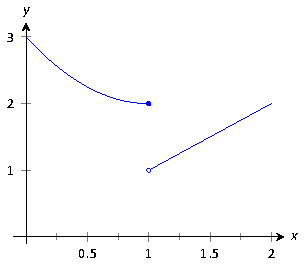
\includegraphics{test-figure2.pdf}
%  \captionof{figure}{Test caption}
%  \end{minipage}}}


%\newenvironment{mfigurefile}[2]{%
%\begin{tikzpicture}[remember picture,overlay]%
%\ifthenelse{\isodd{\thepage}}{\node [xshift=-36pt-.5\marginparwidth,yshift=#2\paperheight] at (current page.south east) }{\node [xshift=36pt+.5\marginparwidth,yshift=#2\paperheight] at (current page.south west) }%
%{\input{#1}};}%
%{\end{tikzpicture}%
%}

%\DeclareCaptionType{mytype}[Typename][List of mytype]


    
%%%%
%% End margin figure 
%%%%    
    

\newcommand{\bmx}[1]{\left[\hskip -3pt\begin{array}{#1} }
\newcommand{\emx}{\end{array}\hskip -3pt\right]}

\newcommand{\btz}{\begin{center}\begin{tikzpicture}}
\newcommand{\etz}{\end{tikzpicture}\end{center}}

\newcommand{\ds}{\displaystyle}

\newcommand{\fp}{\ensuremath{f\,'}}
\newcommand{\fpp}{\ensuremath{f\,''}}

\newcommand{\Fp}{\ensuremath{F\primeskip'}}
\newcommand{\Fpp}{\ensuremath{F\primeskip''}}

\newcommand{\yp}{\ensuremath{y\primeskip'}}
\newcommand{\gp}{\ensuremath{g\primeskip'}}

\newcommand{\dx}{\ensuremath{\Delta x}}
\newcommand{\dy}{\ensuremath{\Delta y}}
%\newcommand{\dz}{\ensuremath{\Delta z}}
\newcommand{\ddz}{\ensuremath{\Delta z}}

\newcommand{\thet}{\ensuremath{\theta}}
\newcommand{\norm}[1]{\ensuremath{||\ #1\ ||}}
\newcommand{\vnorm}[1]{\ensuremath{\norm{\vec #1}}}
\newcommand{\snorm}[1]{\ensuremath{\left|\left|\ #1\ \right|\right|}}
\newcommand{\la}{\left\langle}
\newcommand{\ra}{\right\rangle}
\newcommand{\dotp}[2]{\ensuremath{\vec #1 \cdot \vec #2}}
\newcommand{\proj}[2]{\ensuremath{\text{proj}_{\,\vec #2}{\,\vec #1}}}
\newcommand{\crossp}[2]{\ensuremath{\vec #1 \times \vec #2}}
\newcommand{\veci}{\ensuremath{\vec i}}
\newcommand{\vecj}{\ensuremath{\vec j}}
\newcommand{\veck}{\ensuremath{\vec k}}
\newcommand{\vecu}{\ensuremath{\vec u}}
\newcommand{\vecv}{\ensuremath{\vec v}}
\newcommand{\vecw}{\ensuremath{\vec w}}
\newcommand{\vecx}{\ensuremath{\vec x}}
\newcommand{\vecy}{\ensuremath{\vec y}}
\newcommand{\vrp}{\ensuremath{\vec r\, '}}
\newcommand{\vsp}{\ensuremath{\vec s\, '}}
\newcommand{\vrt}{\ensuremath{\vec r(t)}}
\newcommand{\vst}{\ensuremath{\vec s(t)}}
\newcommand{\vvt}{\ensuremath{\vec v(t)}}
\newcommand{\vat}{\ensuremath{\vec a(t)}}
\newcommand{\px}{\ensuremath{\partial x}}
\newcommand{\py}{\ensuremath{\partial y}}
\newcommand{\pz}{\ensuremath{\partial z}}
\newcommand{\pf}{\ensuremath{\partial f}}
\newcommand{\underlinespace}{\underline{\phantom{xxxxxx}}}

\newcommand{\mathN}{\ensuremath{\mathbb{N}}}

\newcommand{\zerooverzero}{\ensuremath{\ds \raisebox{8pt}{\text{``\ }}\frac{0}{0}\raisebox{8pt}{\text{\ ''}}}}


\newcommand{\myrule}{\rule[-4pt]{0pt}{13pt}}
\newcommand{\mmrule}{\rule[-10pt]{0pt}{15pt}}
\newcommand{\myds}{\ds\mmrule}
\newcommand{\deriv}[2]{\ensuremath{\myds\frac{d}{dx}\left(#1\right)=#2}}
\newcommand{\myint}[2]{\ensuremath{\myds\int #1\ dx=} \ensuremath{\ds #2}}

\DeclareMathOperator{\sech}{sech}
\DeclareMathOperator{\csch}{csch}

\newcommand{\sword}[1]{\textbf{#1}}

\newcommand{\primeskip}{\hskip.75pt}

%%%% Begin Header TikZ

%  Some TiKZ  shortcuts to help make drawing 3D vectors faster.
%

\newcommand{\plotlinecolor}{blue}

%
% Draw x and y tick marks
%
\newcommand{\drawxticks}[1]
{\foreach \x in {#1}
		{\draw  (\x,-.1)--(\x,.1);
			};
}
\newcommand{\drawyticks}[1]
{\foreach \x in {#1}
		{\draw  (-.1,\x)--(.1,\x);
			};
}

\newcommand{\drawxlines}[3]
{\draw[<->] (#1,0) -- (#2,0) node [right] {$x$};
\foreach \x in {#3}
		{\draw  (\x,-.1)--(\x,.1);
			};
}

\newcommand{\drawylines}[3]
{\draw[<->] (0,#1) -- (0,#2) node [above] {$y$};
\foreach \x in {#3}
		{\draw  (-.1,\x)--(.1,\x);
			};
}

\newcommand{\drawxlabels}[1]
{\foreach \x in {#1}
		{\draw  (\x,-.1) node [below] {\scriptsize $\x$};
		};
}

\newcommand{\drawylabels}[1]
{\foreach \x in {#1}
		{\draw  (-.1,\x) node [left] {\scriptsize $\x$};
		};
}

%% draw a box of margin width size to see if figure is properly contained within
\newcommand{\marginsizebox}{\draw (0,0)--(\marginparwidth,0)--(\marginparwidth,3)--(0,3)--cycle;}

%%%%
%%%%

\newcommand{\asyouread}[1]{\begin{tikzpicture}
\ifthenelse{\boolean{in_color}}{\node [preaction={fill=black,opacity=.5,transform canvas={xshift=1mm,yshift=-1mm}}, right color=blue!80!black!30, left color=blue!80] at (0,0) {\textcolor{white}{\textsf{\textit{AS YOU READ $\ldots$}}}};}
{\node [preaction={fill=black,opacity=.5,transform canvas={xshift=1mm,yshift=-1mm}}, right color=black!30, left color=black!10] at (0,0) {\textcolor{white}{\textsf{\textit{AS YOU READ $\ldots$}}}};}
\end{tikzpicture}
\begin{enumerate}
#1
\end{enumerate}
\vskip 20pt}

%%%%
%%  A new figure environment, trying to fix the float problem.
%%
%%%%

\newcounter{myfigurecounter}[chapter]
\renewcommand\themyfigurecounter{\thechapter.\arabic{myfigurecounter}}
\newenvironment{myfigure}{\refstepcounter{myfigurecounter}}{}
\newcommand{\mycaption}[1]{%
\begin{center}%
\vskip -1.5\baselineskip
\begin{tikzpicture}%
\draw (0,0) node [text width=\textwidth,align=center] {Figure \themyfigurecounter: #1};%
\end{tikzpicture}%
\end{center}%
}
\usepackage{pgfplots}
\pgfplotsset{compat=1.8}
\usepackage{pdfpages}

\ifthenelse{\boolean{xetex}}{\renewcommand{\C}{\mathbb{C}}}{\newcommand{\C}{\mathbb{C}}}
\newcommand{\R}{\mathbb{R}}

\ifthenelse{\boolean{xetex}}%
	{\sffamily
	%%\usepackage{fontspec}
	\usepackage{mathspec}
	\setallmainfonts[Mapping=tex-text]{Calibri}
	\setmainfont[Mapping=tex-text]{Calibri}
	\setsansfont[Mapping=tex-text]{Calibri}
	\setmathsfont(Greek){[cmmi10]}}
	{\usepackage[sfdefault,lf]{carlito}
	%% The 'lf' option for lining figures
	%% The 'sfdefault' option to make the base font sans serif
	\usepackage[T1]{fontenc}
	\renewcommand*\oldstylenums[1]{\carlitoOsF #1}}
	
	\ifthenelse{\boolean{luatex}}%
	{\sffamily
	\usepackage{fontspec}
	\usepackage{unicode-math}
	\usepackage{mathspec}
	\setallmainfonts[Mapping=tex-text]{Calibri}
	\setmainfont{Calibri}
	\setsansfont[Mapping=tex-text]{Calibri}
	\setmathfont[range=\mathup]{Calibri}
	\setmathfont[range=\mathit]{Calibri Italic}
	}
	{}
\makeindex
\newcounter{HW}
\newcounter{HWindent}
%%%\tracingonline=1
\begin{document}
%\printexercisenames
\ifthenelse{\boolean{colour}}{\printincolor}{\printinblackandwhite}
%\printincolor
%\printinblackandwhite
%\printallanswers


%
%%%%%%%%%%
%%%
%%%  Set criteria for the format of the book.
%%%  This supercedes anything set in the Text_Header.
%%%
%%%%%%%%%%



%\printinblackandwhite

%\printexercisenames

%\nodrawexamplelines

%\printallanswers


\normalem



%%%\pagenumbering{roman}

%%%%%%
%%%		For editing purposes, block comment down to 
%%%		the next mark
%%%%%%

%%%%\input{cover/front_cover_in_text}
%%%%\clearpage
%%%%\thispagestyle{empty}
\frontmatter
%%%%
%%%%\title{\textsc{Fundamentals of Matrix Algebra}\\
%%%%{\small Version 2.1011}}
%%%%\author{Gregory N. Hartman, Ph.D.}
%%%%\date{}

\vspace*{\stretch{.5}}

\hskip 125pt\begin{minipage}{\textwidth}
\begin{flushright}

\textsc{{\Huge Math 1010 \\
Introduction to Calculus}} \\

\bigskip

\textsl{\Large Fall 2017 Abridged Edition}, 
{\Large University of Lethbridge}\\

%{A version of the \apex\ Calculus textbook edited by }

\bigskip

\Large
\vspace{1in}

\textbf{Editor:} Sean Fitzpatrick

\emph{\large Department of Mathematics and Computer Science}

\emph{\large University of Lethbridge}\vskip15pt

\parbox{200pt}{\textit{Contributing Textbooks}}\hskip 2cm \phantom{.}

\vspace{0.5in}

\textit{Precalculus, Version $\lfloor \pi\rfloor = 3$}

\emph{\large Carl Stitz and Jeff Zeager}

\emph{\large \href{http://www.stitz-zeager.com}{www.stitz-zeager.com}}\vskip 15pt

\apex\ \textit{Calculus}

\emph{\large Gregory Hartman et al}

\emph{\large \href{http://www.apexcalculus.com}{apexcalculus.com}}\vskip 15pt


\normalsize
\end{flushright}
\end{minipage}

\vspace{\stretch{1}}


\thispagestyle{empty}
\clearpage

\vspace*{\stretch{3}}
\noindent\hskip -1in\begin{minipage}{2.2in}
\begin{center}

\includegraphics[width=2in]{figures/license}
\end{center}
\end{minipage}
\begin{minipage}{3.3in}
Chapters 1-4 Copyright \copyright\ 2013 Carl Stitz and Jeff Zeager

Licensed under the Creative Commons Attribution-Noncommercial-ShareAlike 3.0 Unported Public License
\end{minipage}

\bigskip

\bigskip

\bigskip


\noindent\hskip-1in\begin{minipage}{2.2in}
\begin{center}
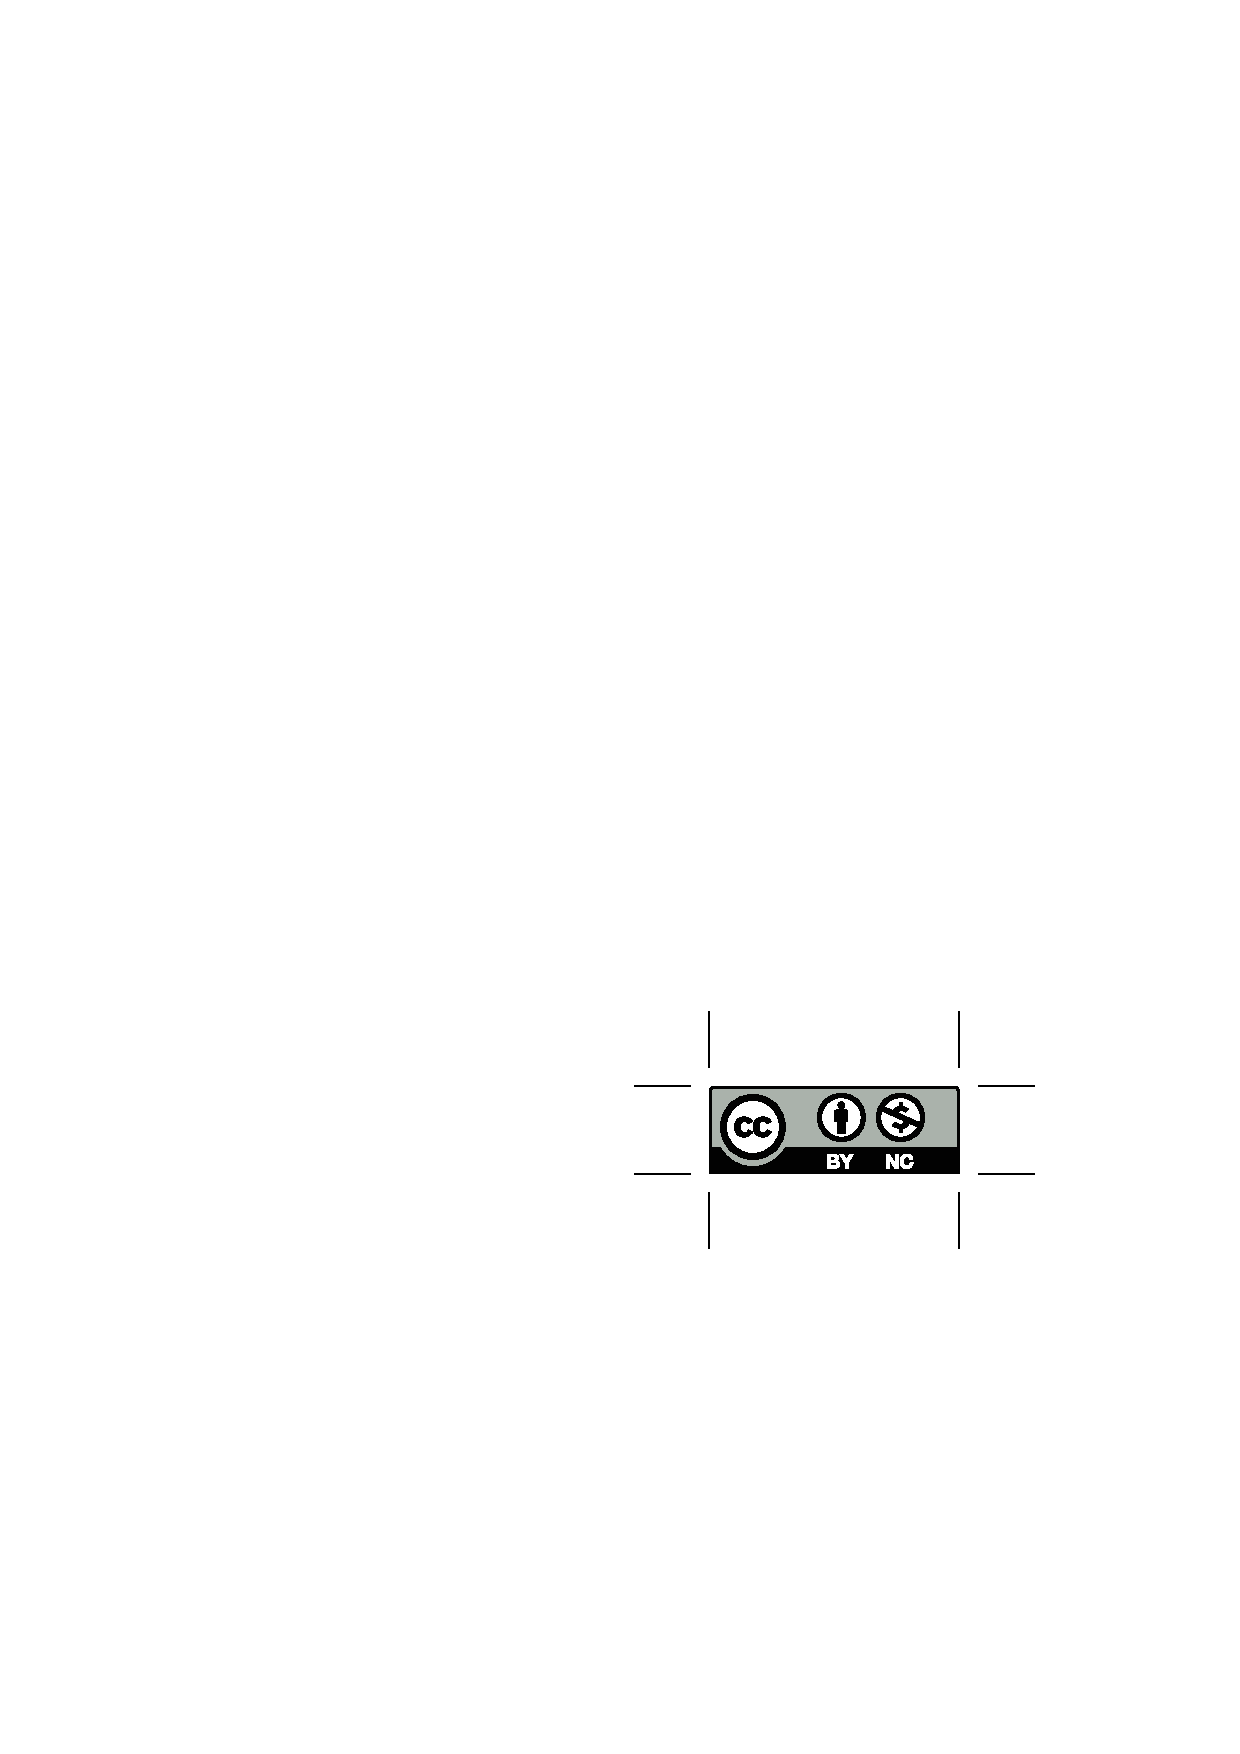
\includegraphics[width=2in]{text/by-nc} 
\end{center}
\end{minipage}
\begin{minipage}{3.3in}
Chapters 5-7 Copyright \copyright\ 2018 Gregory Hartman

Licensed under the Creative Commons Attribution-Noncommercial 4.0 International Public License
\end{minipage}

\bigskip

\bigskip

\bigskip

\noindent\hskip-1in\begin{minipage}{2.2in}
\begin{center}

\includegraphics[width=2in]{figures/license}
\end{center}
\end{minipage}
\begin{minipage}{3.3in}
This version of the text was assembled and edited by Sean Fitzpatrick, University of Lethbridge, July, 2017, and last revised August, 2018.

This work is licensed under the Creative Commons Attribution-Noncommercial-ShareAlike 4.0 International Public License
\end{minipage}
\vspace{\stretch{1}} 
\thispagestyle{empty}
\clearpage
%
%
%\cleardoublepage
%%%%\phantomsection
%%%%\input{text/thanks}
%%%%\addcontentsline{toc}{chapter}{Thanks} 
%%%%\clearpage{\pagestyle{empty}\cleardoublepage}
%%%%\phantomsection
%%%%\thispagestyle{empty}
\Huge
\noindent {\bf \textsc{Preface}}\\
\large
\emph{A Note on Using this Text}
\vspace{1in}
\normalsize

Thank you for reading this short preface. Allow us to share a few key points about the text so that you may better understand what you will find beyond this page.

This text comprises a three--volume series on Calculus. The first part covers material taught in many ``Calc 1'' courses: limits, derivatives, and the basics of integration, found in Chapters 1 through 6.1. The second text covers material often taught in ``Calc 2:'' integration and its applications, along with an introduction to sequences, series and Taylor Polynomials, found in Chapters 5 through 8. The third text covers topics common in ``Calc 3'' or ``multivariable calc:'' parametric equations, polar coordinates, vector--valued functions, and functions of more than one variable, found in Chapters 9 through 13. All three are available separately for free at \texttt{\href{http://apexcalculus.com}{www.apexcalculus.com}}. %These three texts are intended to work together and make one cohesive text, \textit{APEX Calculus}, which can also be downloaded from the website. 

Printing the entire text as one volume makes for a large, heavy, cumbersome book. One can certainly only print the pages they currently need, but some prefer to have a nice, bound copy of the text. Therefore this text has been split into these three manageable parts, each of which can be purchased for under \$15 at \href{http://amazon.com}{Amazon.com}.\\ 



%A result of this splitting is that sometimes a concept is said to be explored in a ``later section,'' though that section does not actually appear in this particular text. Downloading the .pdf of \textit{APEX Calculus} will ensure that you have all the content.  
%material is referenced that is not contained in the present text. The context should make it clear whether the ``missing'' material is in the \textit{Calculus I} or \textit{Calculus III} portion. Downloading the appropriate .pdf, or the whole \textit{APEX Calculus} .pdf, will give access to these topics.
% This splitting of the material also results in unfortunate page/chapter numberings. Chapter 5 of this text is Chapter 1 of \textit{Calculus II}. Apart from these numberings, page--for--page the content of the sections that appear in both \textit{Calculus I} and \textit{Calculus II} are identical.\\ %For instance, in this text, ``Theorem 20'' may be mentioned, although Theorem 20 is only presented in Part I. To minimize confusion, theorems, definitions and key ideas are referenced by their title or subject matter, not their number.

%The current publisher of this text does not allow one text to be split across multiple volumes, with continuity of chapters and page numberings. This is the one drawback of the current publishing model that has many advantages, highlighted below. Because of this, there are a few peculiarities 

\noindent\textbf{\large For Students: How to Read this Text}\\

Mathematics textbooks have a reputation for being hard to read. High--level mathematical writing often seeks to say much with few words, and this style often seeps into texts of lower--level topics. This book was written with the goal of being easier to read than many other calculus textbooks, without becoming too verbose. 

Each chapter and section starts with an introduction of the coming material, hopefully setting the stage for ``why you should care,'' and ends with a look ahead to see how the just--learned material helps address future problems. 

\textit{Please read the text;} it is written to explain the concepts of Calculus. There are numerous examples to demonstrate the meaning of definitions, the truth of theorems, and the application of mathematical techniques. When you encounter a sentence you don't understand, read it again. If it still doesn't make sense, read on anyway, as sometimes confusing sentences are explained by later sentences.

\textit{You don't have to read every equation.} The examples generally show ``all'' the steps needed to solve a problem. Sometimes reading through each step is helpful; sometimes it is confusing. When the steps are illustrating a new technique, one probably should follow each step closely to learn the new technique. When the steps are showing the mathematics needed to find a number to be used later, one can usually skip ahead and see how that number is being used, instead of getting bogged down in reading how the number was found.

\textit{Most proofs have been omitted.} In mathematics, \textit{proving} something is always true is extremely important, and entails much more than testing to see if it works twice. However, students often are confused by the details of a proof, or become concerned that they should have been able to construct this proof on their own. To alleviate this potential problem, we do not include the proofs to most theorems in the text. The interested reader is highly encouraged to find proofs online or from their instructor. In most cases, one is very capable of understanding what a theorem \textit{means} and \textit{how to apply it} without knowing fully \textit{why} it is true.
\\

\thispagestyle{empty}
\noindent\textbf{\large Interactive, 3D Graphics}\\

New to Version 3.0 is the addition of interactive, 3D graphics in the .pdf version. Nearly all graphs of objects in space can be rotated, shifted, and zoomed in/out so the reader can better understand the object illustrated. 

As of this writing, the only pdf viewers that support these 3D graphics are Adobe Reader \& Acrobat (and only the versions for PC/Mac/Unix/Linux computers, not tablets or smartphones). To activate the interactive mode, click on the image. Once activated, one can click/drag to rotate the object and use the scroll wheel on a mouse to zoom in/out. (A great way to investigate an image is to first zoom in on the page of the pdf viewer so the graphic itself takes up much of the screen, then zoom inside the graphic itself.) A CTRL-click/drag pans the object left/right or up/down. By right-clicking on the graph one can access a menu of other options, such as changing the lighting scheme or perspective. One can also revert the graph back to its default view. If you wish to deactive the interactivity, one can right-click and choose the ``Disable Content'' option. \\

\noindent\textbf{\large Thanks}\\

There are many people who deserve recognition for the important role they have played in the development of this text. First, I thank Michelle for her support and encouragement, even as this ``project from work'' occupied my time and attention at home. Many thanks to Troy Siemers, whose most important contributions extend far beyond the sections he wrote or the 227 figures he coded in Asymptote for 3D interaction.  He provided incredible support, advice and encouragement for which I am very grateful. My thanks to Brian Heinold and Dimplekumar Chalishajar for their contributions and to Jennifer Bowen for reading through so much material and providing great feedback early on. Thanks to Troy, Lee Dewald, Dan Joseph, Meagan Herald, Bill Lowe, John David, Vonda Walsh, Geoff Cox, Jessica Libertini and other faculty of VMI who have given me numerous suggestions and corrections based on their experience with teaching from the text. (Special thanks to Troy, Lee \& Dan for their patience in teaching Calc III while I was still writing the Calc III material.) Thanks to Randy Cone for encouraging his tutors of VMI's Open Math Lab to read through the text and check the solutions, and thanks to the tutors for spending their time doing so. A very special thanks to Kristi Brown and Paul Janiczek who took this opportunity far above \& beyond what I expected, meticulously checking every solution and carefully reading every example. Their comments have been extraordinarily helpful. I am also thankful for the support provided by Wane Schneiter, who as my Dean provided me with extra time to work on this project. I am blessed to have so many people give of their time to make this book better.\\

\noindent\textbf{\large \apex\  -- Affordable Print and Electronic teXts}\\

\apex\ is a consortium of authors  who collaborate to produce high--quality, low--cost textbooks. The current textbook--writing paradigm is facing a potential revolution as desktop publishing and electronic formats increase in popularity. However, writing a good textbook is no easy task, as the time requirements alone are substantial. It takes countless hours of work to produce text, write examples and exercises, edit and publish. Through collaboration, however, the cost to any individual can be lessened, allowing us to create texts that we freely distribute electronically and sell in printed form for an incredibly low cost. Having said that, nothing is entirely free; someone always bears some cost. This text ``cost'' the authors of this book their time, and that was not enough. \textit{APEX Calculus} would not exist had not the Virginia Military Institute, through a generous Jackson--Hope grant, given the lead author significant time away from teaching so he could focus on this text.

Each text is available as a free .pdf, protected by a Creative Commons Attribution - Noncommercial 4.0 copyright. That  means you can give the .pdf to anyone you like, print it in any form you like, and even edit the original content and redistribute it. If you do the latter, you must  clearly reference this work and you cannot sell your edited work for money.

We encourage others to adapt this work to fit their own needs. One might add sections that are ``missing'' or remove sections that your students won't need. The source files can be found at \texttt{\href{https://github.com/APEXCalculus}{github.com/APEXCalculus}}.

You can learn more at \texttt{\href{http://www.vmi.edu/APEX}{www.vmi.edu/APEX}}.
\thispagestyle{empty}


%%%%\addcontentsline{toc}{chapter}{Preface}
%%%%\clearpage{\pagestyle{empty}\cleardoublepage}
%%%%\phantomsection
%
% The following is the correct TOC; the 
%
%%%%

\addtocontents{toc}{\protect\thispagestyle{empty}}
\addcontentsline{toc}{chapter}{Table of Contents}
\tableofcontents
\clearpage{\pagestyle{empty}\cleardoublepage}

\phantomsection
\prefacegeometry
\addcontentsline{toc}{chapter}{Preface}
\thispagestyle{empty}
\Huge
\noindent {\bf \textsc{Preface}}\\
\normalsize

One of the challenges with a new course like Math 1010 is finding a suitable textbook for the course. This is made additionally difficult for a course that covers two topics -- Precalculus and Calculus -- that are usually offered as separate courses, with separate texts. I reviewed a number of commercially available options, but these all had two things in common: they did not quite meet our needs, and they were all very expensive (some were as much as \$400).

Since writing a new textbook from scratch is a huge undertaking, requiring resources (like time) we simply did not have, I chose to explore non-commercial options. This took a bit of searching, since non-commercial texts, while inexpensive (or free), are of varying quality. Fortunately, there are some decent texts out there. Unfortunately, I couldn't find a single text that covered all of the material we need for Math 1010.

To get around this problem, I have selected two textbooks as our primary sources for the course. The first is \textit{Precalculus}, version 3, by Carl Stitz and Jeff Zeager. The second is \textit{APEX Calculus I},  version 3.0, by Hartman et al. Both texts have two very useful advantages. First, they're both free (as in beer): you can download either text in PDF format from the authors' web pages. Second, they're also \textit{open source} texts (that is, free, as in speech). Both books are written using the \LaTeX markup language, as is typical in mathematics publishing. What is not typical is that the authors of both texts make their source code freely available, allowing others (such as myself) to edit and customize the books as they see fit.

In the first iteration of this project (Fall 2015), I was only able to edit each text individually for length and content, resulting in two separate textbooks for Math 1010. This time around, I've had enough time to take the content of the Precalculus textbook and adapt its source code to be compatible with the formatting of the Calculus textbook, allowing me to produce a single textbook for all of Math 1010.

This is a much shortened, abridged version of the ``Complete (and Current) Edition'' produced last summer. That version has more material than an instructor can reasonably expect to cover in one semester. It is still available for a student who wants a more complete treatment of the precalculus material in the text.

The book is very much a work in progress, and I will be editing it regularly. Feedback is always welcome. 

\newpage

\noindent\textbf{\large Acknowledgements}\\

First and foremost, I need to thank the authors of the two textbooks that provide the source material for this text. Without their hard work, and willingness to make their books (and the source code) freely available, it would not have been possible to create an affordable textbook for this course. You can find the original textbooks at their websites:

\bigskip


\href{http://www.stitz-zeager.com}{www.stitz-zeager.com}, for the \textit{Precalculus} textbook, by Stitz and Zeager, and

\bigskip


\href{http://www.apexcalculus.com}{apexcalculus.com}, for the \apex\ \textit{Calculus} textbook, by Hartman et al.

\bigskip

I'd also like to thank Dave Morris for help with converting the graphics in the Precalculus textbook to work with the formatting code of the APEX text, Howard Cheng for providing some C++ code to convert the exercises, and the other faculty members involved with this course --- Alia Hamieh, David Kaminsky, and Nicole Wilson --- for their input on the content of the text.

\vspace{1in}

\begin{raggedright}
Sean Fitzpatrick\\
Department of Mathematics and Computer Science\\
University of Lethbridge\\
July, 2017
\end{raggedright}





\restoregeometry
\clearpage{\pagestyle{empty}\cleardoublepage}

%%%%%
%\includepdf[pages={1,2}]{CalculusTOC.pdf}

%%%%
\mainmatter


%%%%
%		End block comment here
%%%%






\clearpage{\pagestyle{empty}\cleardoublepage}
\chapter{The Real Numbers}\label{chapter:reals}
\thispagestyle{empty}


\section{Some Basic Set Theory Notions}
\label{SetTheory}

%\label{SetTheoryNotions}


%\label{SetsofNumbers}
While the authors would like nothing more than to delve quickly and deeply into the sheer excitement that is \textit{Precalculus}, experience has taught us that a brief refresher on some basic notions is welcome, if not completely necessary, at this stage.  To that end, we present a brief summary of `set theory' and some of the associated vocabulary and notations we use in the text. Like all good Math books, we begin with a definition.


\definition{setdef}{Set}{
A \sword{set}\index{set ! definition of} is a well-defined collection of objects which are called the `elements' of the set.  Here, `well-defined' means that it is possible to determine if something belongs to the collection or not, without prejudice. 
}

\smallskip

For example, the collection of letters that make up the word ``pronghorns'' is well-defined and is a set, but  the collection of the worst math teachers in the world is \textbf{not} well-defined, and so is \textbf{not} a set.  In general, there are three ways to describe sets.  They are

\mnote{.55}{One thing that student evaluations teach us is that any given Mathematics instructor can be simultaneously the best and worst teacher ever, depending on who is completing the evaluation.}

\smallskip

\keyidea{idea:setdescription}{Ways to Describe Sets}{
\begin{enumerate}

\item \textbf{The Verbal Method:} Use a sentence to define a set.\index{set ! verbal description}

\item \textbf{The Roster Method:}  Begin with a left brace `$\{$', list each element of the set \textit{only once} and then end with a right brace `$\}$'.\index{set ! roster method}

\item \textbf{The Set-Builder Method:} A combination of the verbal and roster methods using a ``dummy variable'' such as $x$.\index{set ! set-builder notation}\index{set-builder notation}

\end{enumerate}
}
\smallskip

For example, let $S$ be the set described \textit{verbally} as the set of letters that make up the word ``pronghorns''.  A  \sword{roster} description of $S$ would be  $\left\{ p, r, o, n, g, h, s \right\}$. Note that we listed `r', `o', and `n' only once, even though they appear twice in ``pronghorns.''  Also, the \textit{order} of the elements doesn't matter, so $\left\{ o, n, p, r, g, s, h \right\}$ is also a roster description of $S$.   A \sword{set-builder} description of $S$ is: \[ \{ x \, | \, \mbox{$x$ is a
letter in the word ``pronghorns''.}\} \]

The way to read this is: `The set of elements $x$ \underline{such that} $x$ is a letter in the word ``pronghorns.'''   In each of the above cases, we may use the familiar equals sign `$=$' and write  $S = \left\{  p, r, o, n, g, h, s  \right\}$ or $S = \{ x \, | \, \mbox{$x$ is a
letter in the word ``pronghorns''.}\}$.  Clearly $r$ is in $S$ and $q$ is not in $S$.  We express these sentiments mathematically by writing  $r \in S$ and $q \notin S$. 

More precisely, we have the following.

\medskip

\definition{notationforsetinclusion}{Notation for set inclusion}{ Let $A$ be a set.

\begin{itemize}

\item If $x$ is an element of $A$ then we write $x \in A$\index{set ! inclusion}\index{$\in$} which is read `$x$ is in $A$'.

\item If $x$ is \emph{not} an element of $A$ then we write $x \notin A$\index{set ! exclusion}\index{$\notin$} which is read `$x$ is not in $A$'.

\end{itemize}
}

\medskip

Now let's consider the set $C =  \{ x \, | \, \mbox{$x$ is a consonant in the word ``pronghorns''}\}$.  A roster description of $C$ is  $C = \{ p, r, n, g, h, s\}$.  Note that by construction, every element of $C$ is also in $S$.  We express this relationship by stating that the set $C$ is a \textbf{subset} of the set $S$, which is written in symbols as $C \subseteq S$.  The more formal definition is given below.

\medskip

\definition{subsetdef}{Subset}{
Given sets $A$ and $B$, we say that the set $A$ is a \textbf{subset}\index{subset ! definition of} of the set $B$ and write `$A \subseteq B$' if every element in $A$ is also an element of $B$.  
}

\medskip

Note that in our example above $C \subseteq S$, but not vice-versa, since $o \in S$ but $o \notin C$.  Additionally, the set of vowels $V = \{ a, e, i, o, u\}$, while it does have an element in common with $S$, is not a subset of $S$. (As an added note,  $S$ is not a subset of $V$, either.)  We could, however, \textit{build} a set which contains both $S$ and $V$ as subsets by gathering all of the elements in both $S$ and $V$ together into a single set, say $U = \{ p, r, o, n, g, h, s, a, e, i, u\}$.   Then $S \subseteq U$ and $V \subseteq U$.  The set $U$ we have built is called the \textbf{union} of the sets $S$ and $V$ and is denoted $S \cup V$.    Furthermore, $S$ and $V$ aren't completely \textit{different} sets since they both contain the letter `o.' (Since the word `different' could be ambiguous, mathematicians use the word \textit{disjoint} to refer to two sets that have no elements in common.) The \textbf{intersection} of two sets is the set of elements (if any) the two sets have in common. In this case, the intersection of $S$ and $V$ is $\{ o\}$, written $S \cap V = \{ o \}$.  We formalize these ideas below.

\medskip

\definition{intersectionunion}{Intersection and Union}{
 Suppose $A$ and $B$ are sets.

\begin{itemize}

\item The \textbf{intersection}\index{set ! intersection}\index{intersection of two sets} of $A$ and $B$ is $A \cap B = \{ x \, | \, x \in A \, \text{and} \,\, x \in B \}$

\item The \textbf{union}\index{set ! union}\index{union of two sets} of $A$ and $B$ is $A \cup B = \{ x \, | \, x \in A \, \text{or} \,\, x \in B \, \, \text{(or both)} \}$

\end{itemize}
}

\medskip

The key words in Definition \ref{intersectionunion} to focus on are the conjunctions:  `intersection' corresponds to `and' meaning the elements have to be in \textit{both} sets to be in the intersection, whereas `union' corresponds to `or' meaning the elements have to be in one set, or the other set (or both).  In other words, to belong to the union of two sets an element must belong to \textit{at least one} of them.

\smallskip

Returning to the sets $C$ and $V$  above, $C \cup V = \{ p, r, n, g, h, s, a, e, i, o, u\}$. When it comes to their intersection, however, we run into a bit of notational awkwardness since $C$ and $V$ have no elements in common.  While we could write $C \cap V = \{ \}$, this sort of thing happens often enough that we give the set with no elements a name. 

\medskip

\definition{emptysetdefn}{Empty set}{
The \textbf{Empty Set} $\emptyset$ is the set which contains no elements.\index{set ! empty}\index{empty set}  That is, \[\emptyset=\{ \}=\{x\,|\,\mbox{$x \neq x$}\}.\]  
}

\medskip

As promised, the empty set is the set containing no elements since no matter what `$x$' is, `$x = x$.'  Like the number `$0$,'  the empty set plays a vital role in mathematics. We introduce it here more as a symbol of convenience as opposed to a contrivance.
\mnote{.85}{The full extent of the empty set's role will not be explored in this text, but it is of fundamental importance in Set Theory. In fact, the empty set can be used to generate numbers -  mathematicians can create something from nothing! If you're interested, read about the \href{https://en.wikipedia.org/wiki/Natural_number\#von_Neumann_construction}{von Neumann construction of the natural numbers} or consider signing up for Math 2000.}   
Using this new bit of notation, we have for the sets $C$ and $V$ above that $C \cap V = \emptyset$.    A nice way to visualize relationships between sets and set operations is to draw a  \href{http://en.wikipedia.org/wiki/Venn_diagram}{\underline{\textbf{Venn Diagram}}}\index{diagram ! Venn Diagram}\index{Venn Diagram}.  A Venn Diagram for the sets $S$, $C$ and $V$ is drawn in Figure \ref{venndiagram}.

\mtable{.68}{A Venn diagram for $C$, $S$, and $V$}{venndiagram}{
\myincludegraphics[width=0.95\marginparwidth]{figures/RelationsandFunctionsGraphics/SetTheory-1}
}

In Figure \ref{venndiagram} we have three circles - one for each of the sets $C$, $S$ and $V$.  We visualize the area enclosed by each of these circles as the elements of each set.  Here, we've spelled out the elements for definitiveness.  Notice that the circle representing the set $C$ is completely inside the circle representing $S$.  This is a geometric way of  showing that $C \subseteq S$.  Also, notice that the circles representing $S$ and $V$ overlap on the letter `o'.  This common region is how we visualize $S \cap V$.  Notice that since $C \cap V = \emptyset$, the circles which represent $C$ and $V$ have no overlap whatsoever.  

\medskip

All of these circles lie in a rectangle labelled $U$ (for `universal' set).  A universal set contains all of the elements under discussion, so it could always be taken as the union of all of the sets in question, or an even larger set.  In this case, we could take $U = S \cup V$ or $U$ as the set of letters in the entire alphabet.    The usual triptych of Venn Diagrams indicating generic sets $A$ and  $B$ along with $A \cap B$ and $A \cup B$ is given below.

(The reader may well wonder if there is an ultimate universal set which contains \textit{everything}.  The short answer is `no'. Our definition of a set turns out to be overly simplistic, but correcting this takes us well beyond the confines of this course. If you want the longer answer, you can begin by reading about \href{http://en.wikipedia.org/wiki/Russell's_paradox}{\underline{Russell's Paradox}} on Wikipedia.)

\mtable{.32}{Venn diagrams for intersection and union}{fig:intunion}{
\begin{tabular}{c}
\myincludegraphics[scale=0.8]{figures/RelationsandFunctionsGraphics/SetTheory-2}\\
Sets $A$ and $B$.\\
\\
\myincludegraphics[scale=0.8]{figures/RelationsandFunctionsGraphics/SetTheory-3}\\
$A\cap B$ is shaded.\\
\\
\myincludegraphics[scale=0.8]{figures/RelationsandFunctionsGraphics/SetTheory-4}\\
$A\cup B$ is shaded.
\end{tabular}
}

\subsection{Sets of Real Numbers}
\label{SetsofNumbers}

The playground for most of this text is the set of \textbf{Real Numbers}.  Many quantities in the `real world' can be quantified using real numbers: the temperature at a given time, the revenue generated by selling a certain number of products and the maximum population of Sasquatch which can inhabit a particular region are just three basic examples.   A succinct, but nonetheless incomplete definition of a real number is given below.

\medskip

\definition{realnumberdefn}{The real numbers}{

A \sword{real number}\index{real number ! set of}\index{real number ! definition of} is any number which possesses a decimal representation.  The set of real numbers is denoted by the character $\mathbb{R}$.
}

\medskip

Certain subsets of the real numbers are worthy of note and are listed below.  In more advanced courses like Analysis, you learn that the real numbers can be {\em constructed} from the rational numbers, which in turn can be constructed from the integers (which themselves come from the natural numbers, which in turn can be defined as sets...).

\medskip

\phantomsection
\label{setsofnumbersboxonthispage}
\setboxwidth{30pt}
\noindent\hskip-12pt
\begin{minipage}{1.2\linewidth}
\definition{def:numbersets}{Sets of Numbers}{\index{set ! sets of numbers}

\begin{enumerate}

\item The \sword{Empty Set}:\index{set ! empty}\index{empty set} $\emptyset=\{ \}=\{x\,|\,\mbox{$x
\neq x$}\}$.  This is the set with no elements.  Like the number `$0$,' it  plays a vital role in mathematics.

\item The \sword{Natural Numbers}:\index{natural number ! set of}\index{natural number ! definition of} $\mathbb N= \{ 1, 2, 3,  \ldots\}$ The periods of ellipsis here indicate that the natural numbers contain $1$, $2$, $3$, `and so forth'.

%\item The \sword{Whole Numbers}:\index{whole number ! set of}\index{whole number ! definition of} $\mathbb W = \{ 0, 1, 2, \ldots \}$

\item The \sword{Integers}:\index{integer ! set of}\index{integer ! definition of} $\mathbb Z=\{ \ldots, -3, -2, -1, 0, 1, 2, 3, \ldots \}$

\item The \sword{Rational Numbers}:\index{rational number ! set of}\index{rational number ! definition of} $\mathbb Q=\left\{\frac{a}{b} \, | \, a \in \mathbb Z \, \mbox{and} \, b \in \mathbb Z \right\}$.  \underline{Ratio}nal numbers are the \underline{ratio}s of integers (provided the denominator is not zero!)  It turns out that another way to describe the rational numbers is: \[\mathbb Q=\{x\,|\,\mbox{$x$ possesses a repeating or terminating decimal representation.}\}\]

\item The \sword{Real Numbers}:\index{real number ! set of}\index{real number ! definition of} $\mathbb R = \{ x\,|\,\mbox{$x$ possesses a decimal representation.}\}$

\item The \sword{Irrational Numbers}:\index{irrational number ! set of}\index{irrational number ! definition of} Real numbers that are not rational are called \sword{irrational}.  As a set, we have  $\{x\in\mathbb{R}\,|\, x\notin \mathbb{Q}\}$. (There is no standard symbol for this set.)  Every \underline{ir}rational number has a decimal expansion which neither repeats nor terminates.

\item The \sword{Complex Numbers}:\index{complex number ! set of}\index{complex number ! definition of} $\mathbb C=\{a+bi\,|\,\mbox{$a$,$b \in \mathbb R$ and $i=\sqrt{-1}$}\}$  (We will not deal with complex numbers in Math 1010, although they usually make an appearance in Math 1410.)

\end{enumerate}
}
\end{minipage}
\restoreboxwidth
%\enlargethispage{.05in}

\medskip

\mnote{.65}{An example of a number with a repeating decimal expansion is $a=2.13234234234\ldots$. This is rational since $100a = 213.2342342342...$, and $100000a = 213234.234234...$ so $99900a = 100000a-100a = 213021$. This gives us the rational expression $a = \dfrac{213021}{99900}$.}
\mnote{.52}{The classic example of an irrational number is the number $\pi$, but numbers like $\sqrt{2}$ and $0.101001000100001\ldots$ are other fine representatives.}

\medskip


It is important to note that every natural number is a whole number is an integer.   Each integer is a rational number (take $b =1$ in the above definition for $\mathbb Q$) and the rational numbers are all real numbers, since they possess decimal representations (via long division!). If we take $b=0$ in the above definition of $\mathbb C$, we see that every real number is a complex number.  In this sense, the sets $\mathbb N$, $\mathbb Z$, $\mathbb Q$, $\mathbb R$, and $\mathbb C$ are `nested' like \href{http://en.wikipedia.org/wiki/Matryoshka_doll}{\underline{Matryoshka dolls}}. More formally, these sets form a subset chain:  $\mathbb{N} \subseteq \mathbb Z \subseteq \mathbb{Q} \subseteq \mathbb{R}$.  The reader is encouraged to sketch a Venn Diagram depicting $\mathbb{R}$ and all of the subsets mentioned above.  

\medskip

As you may recall, we often visualize the set of real numbers $\mathbb{R}$ as a line where each point on the line corresponds to one and only one real number.  Given two different real numbers $a$ and $b$,  we write $a < b$ if $a$ is located to the left of $b$ on the number line, as shown in Figure \ref{fig:numline}.




While this notion seems innocuous, it is worth pointing out that this convention is rooted in two deep properties of real numbers.  The first property is that $\mathbb{R}$ is  \href{http://en.wikipedia.org/wiki/Complete_metric_space}{\underline{complete}}. This means that there are no `holes' or `gaps' in the real number line. (This intuitive feel for what it means to be `complete' is as good as it gets at this level.  Completeness does get a much more precise meaning later in courses like Analysis and Topology.) Another way to think about this is that if you choose any two distinct (different) real numbers, and look between them, you'll find a solid line segment (or interval) consisting of infinitely many real numbers.  



The next result tells us what types of numbers we can expect to find.

\medskip

\theorem{densityofqandp}{Density Property of $\mathbb{Q}$ in $\mathbb{R}$}{

Between any two distinct real numbers, there is at least one rational number and irrational number.  It then follows that between any two distinct real numbers there will be \underline{infinitely many} rational and irrational numbers.
}

\medskip

The root word `dense' here communicates the idea that rationals and irrationals are `thoroughly mixed' into $\mathbb{R}$.   The reader is encouraged to think about how one would find both a rational and an irrational number between, say, $0.9999$ and $1$. Once you've done that, ask yourself whether there is any difference between the numbers $0.\overline{9}$ and $1$. 

\smallskip

\mfigure{.5}{The real number line with two numbers $a$ and $b$, where $a<b$.}{fig:numline}{figures/RelationsandFunctionsGraphics/SetTheory-5}

The second property $\mathbb{R}$ possesses that lets us view it as a line is that the set is \href{http://en.wikipedia.org/wiki/Total_order}{\underline{totally ordered}}. This means that given any two real numbers $a$ and $b$, either $a < b$, $a > b$ or $a = b$ which allows us to arrange the numbers from least (left) to greatest (right). You may have heard this property given as the `Law of Trichotomy'.\index{trichotomy}

\medskip

\definition{trichotomy}{Law of Trichotomy}{
If $a$ and $b$ are real numbers then {\bf exactly one} of the following statements is true: \vspace{-.15in} 
\[
  \begin{array}{lclcl}
  a < b & \hspace*{1.25in} & a > b & \hspace*{1.25in} & a = b 
  \end{array} 
\]
}
\mnote{.35}{The Law of Trichotomy, strictly speaking, is an \textit{axiom} of the real numbers: a basic requirement that we assume to be true. However, in any \textit{construction} of the real numbers, such as the method of \href{https://en.wikipedia.org/wiki/Dedekind_cut}{Dedekind cuts}, it is necessary to \textit{prove} that the Law of Trichotomy is satisfied.}

\medskip

The reader is probably familiar with the relations $a<b$ and $a>b$ in the context of \textit{solving inequalities}. The \textbf{order properties} of the real number system can be summarized as a collection of rules for manipulating inequalities, as follows:\\

\keyidea{inequalityrules}{Rules for inequalities}{
Let $a$, $b$, and $c$ be any real numbers. Then:
\begin{itemize}
\item If $a<b$, then $a+c<b+c$.
\item If $a<b$, then $a-c<b-c$.
\item If $a<b$ \textbf{and} $c>0$, then $ac<bc$.
\item If $a<b$ and $c<0$, then $ac>bc$. (In particular, $-a>-b$.)
\item If $0<a<b$, then $\dfrac{1}{b}<\dfrac{1}{a}$.
\end{itemize}
}

Note the emphasis in rule \#3 above: caution must always be exercised when manipulating inequalities: multiplying by a negative number reverses the sign. This is especially important to remember when dealing with inequalities involving variable quantities, for example, with rational inequalities (see Example \ref{ex_ratineq}).

\medskip

 Segments of the real number line are called \sword{intervals}\index{interval ! definition of} of numbers. Below is a summary of the so-called \sword{interval notation}\index{interval ! notation for} associated with given sets of numbers.  For intervals with finite endpoints, we list the left endpoint, then the right endpoint.  We use square brackets, `$[$' or `$]$', if the endpoint is included in the interval and use a filled-in or `closed' dot to indicate membership in the interval. Otherwise, we use parentheses, `$($' or `$)$' and an `open' circle to indicate that the endpoint is not part of the set.  If the interval does not have finite endpoints, we use the symbols $-\infty$ to indicate that the interval extends indefinitely to the left and $\infty$ to indicate that the interval extends indefinitely to the right.  Since infinity is a concept, and not a number, we always use parentheses when using these symbols in interval notation, and use an appropriate arrow to indicate that the interval extends indefinitely in one (or both) directions.

\medskip
\setboxwidth{10pt}
\noindent\begin{minipage}{1.1\linewidth}
\definition{def:intervalnot}{Interval Notation}{
Let $a$ and $b$ be real numbers with $a<b$.

\smallskip

%\begin{center}

\noindent\hskip-10pt\begin{tabular}{|c|c|c|} \hline

Set of Real Numbers & Interval Notation &  Region on the Real Number Line  \\
\hline

 &  & \\
\shortstack{$\{x\,|\,a<x<b\}$ \\ \hfill}& \shortstack{$(a,b)$ \\ \hfill} & 

\myincludegraphics{figures/RelationsandFunctionsGraphics/CartesianPlane-1}  \\ \hline

& &  \\
\shortstack{$\{x\,|\,a\leq x<b\}$ \\ \hfill}& \shortstack{$[a,b)$ \\ \hfill} & 

\myincludegraphics{figures/RelationsandFunctionsGraphics/CartesianPlane-2}   \\
\hline

 &  & \\
\shortstack{$\{x\,|\,a<x\leq b\}$ \\ \hfill}&\shortstack{$(a,b]$ \\ \hfill} & 

\myincludegraphics{figures/RelationsandFunctionsGraphics/CartesianPlane-3}   \\
\hline

 &  & \\
\shortstack{$\{x\,|\,a\leq x \leq b\}$ \\ \hfill}& \shortstack{$[a,b]$ \\ \hfill}& 

\myincludegraphics{figures/RelationsandFunctionsGraphics/CartesianPlane-4}   \\
\hline

 & & \\
\shortstack{$\{x\,| \, x<b\}$ \\ \hfill}& \shortstack{$(-\infty,b)$ \\ \hfill}& 

\myincludegraphics{figures/RelationsandFunctionsGraphics/CartesianPlane-5}   \\
\hline


&  & \\

\shortstack{$\{x\,| \, x \leq b\}$ \\ \hfill} & \shortstack{$(-\infty,b]$ \\ \hfill}& 

\myincludegraphics{figures/RelationsandFunctionsGraphics/CartesianPlane-6}   \\
\hline

 &  & \\
\shortstack{$\{x\,| \, x>a\}$ \\ \hfill}& \shortstack{$(a,\infty)$ \\ \hfill}& 

\myincludegraphics{figures/RelationsandFunctionsGraphics/CartesianPlane-7}   \\
\hline

 &  & \\
\shortstack{$\{x\,| \, x \geq a \}$ \\ \hfill}& \shortstack{$[a,\infty)$ \\ \hfill} & 

\myincludegraphics{figures/RelationsandFunctionsGraphics/CartesianPlane-8}   \\
\hline

&  & \\
\shortstack{$\mathbb R$ \\ \hfill}& \shortstack{$(-\infty,\infty)$ \\ \hfill} & 

\myincludegraphics{figures/RelationsandFunctionsGraphics/CartesianPlane-9}   \\
\hline

\end{tabular}

%\end{center}
}
\end{minipage}
%\pagebreak
\restoreboxwidth

\medskip


As you can glean from the table, for intervals with finite endpoints we start by writing `left endpoint, right endpoint'.  We use square brackets, `$[$' or `$]$', if the endpoint is included in the interval. This corresponds to a `filled-in' or `closed' dot on the number line to indicate that the number is included in the set.  Otherwise, we use parentheses, `$($' or `$)$' that correspond to an `open' circle which indicates that the endpoint is not part of the set.  If the interval does not have finite endpoints, we use the symbol $-\infty$ to indicate that the interval extends indefinitely to the left and the symbol $\infty$ to indicate that the interval extends indefinitely to the right.  Since infinity is a concept, and not a number, we always use parentheses when using these symbols in interval notation, and use the appropriate arrow to indicate that the interval extends indefinitely in one or both directions. 

\mnote{.5}{The importance of understanding interval notation in Calculus cannot be overstated. If you don't find yourself getting the hang of it through repeated use, you may need to take the time to just memorize this chart.} 

Let's do a few examples to make sure we have the hang of the notation:

\medskip




\begin{center}
\begin{tabular}{|c|c|c|} \hline

Set of Real Numbers & Interval Notation &  Region on the Real Number Line  \\
\hline

& &  \\
\shortstack{$\{x\,|\,1\leq x< 3\}$ \\ \hfill} & \shortstack{$[1,3)$ \\ \hfill} & 

\myincludegraphics{figures/RelationsandFunctionsGraphics/CartesianPlane-10}  \\
\hline

 &  & \\
\shortstack{$\{x\,|\,-1\leq x \leq 4\}$ \\ \hfill}& \shortstack{$[-1,4]$ \\ \hfill} & 

\myincludegraphics{figures/RelationsandFunctionsGraphics/CartesianPlane-11}   \\
\hline

&  & \\

\shortstack{$\{x\,| \, x \leq 5 \}$ \\ \hfill} & \shortstack{$(-\infty, 5]$ \\ \hfill} &

\myincludegraphics{figures/RelationsandFunctionsGraphics/CartesianPlane-12}   \\
\hline

 &  & \\
\shortstack{$\{x\,| \, x > -2 \}$ \\ \hfill} & \shortstack{$(-2, \infty)$ \\ \hfill} &  

\myincludegraphics{figures/RelationsandFunctionsGraphics/CartesianPlane-13}   \\
\hline

\end{tabular}

\end{center}


\medskip

We defined the intersection and union of arbitrary sets in Definition \ref{intersectionunion}. Recall that  the union of two sets consists of the totality of the elements in each of the sets, collected together. For example,  if $A = \{ 1,2,3 \}$ and $B = \{2,4,6 \}$, then $A \cap B = \{2\}$ and $A \cup B = \{1,2,3,4,6\}$.   If $A = [-5,3)$ and $B = (1, \infty)$, then we can find $A \cap B$ and $A\cup B$ graphically.  To find $A\cap B$, we shade  the overlap of the two and obtain $A \cap B = (1,3)$.  To find $A \cup B$, we shade each of $A$ and $B$ and describe the resulting shaded region to find  $A \cup B = [-5,\infty)$.

\mtable{.75}{Union and intersection of intervals}{fig:venn1}{%
\begin{tabular}{c}
\myincludegraphics{figures/RelationsandFunctionsGraphics/CartesianPlane-14}\\
$A = [-5,3)$,  $B = (1, \infty)$\\
\\
\myincludegraphics{figures/RelationsandFunctionsGraphics/CartesianPlane-15}\\
$A \cap B = (1,3)$\\
\\
\myincludegraphics{figures/RelationsandFunctionsGraphics/CartesianPlane-16}\\
$A \cup B = [-5,\infty)$
\end{tabular}
}


While both intersection and union are important, we have more occasion to use union in this text than intersection, simply because most of the sets of real numbers we will be working with are either intervals or are unions of intervals, as the following example illustrates.

\medskip


\example{unionex}{Expressing sets as unions of intervals}{
Express the following sets of numbers using interval notation.

\begin{multicols}{2}

\begin{enumerate}

\item  $\{ x \, | \, x \leq -2 \, \, \text{or} \, \,  x \geq 2 \}$

\item  $\{ x \, | \, x \neq 3 \}$

%\setcounter{HW}{\value{enumi}}

\end{enumerate}

\end{multicols}

\begin{multicols}{2}

\begin{enumerate}

\setcounter{enumi}{2}

\item  $\{ x \, | \, x \neq \pm 3 \}$

\item  $\{ x \, | \, -1 < x \leq 3 \,\, \text{or} \,\, x = 5\}$

\end{enumerate}

\end{multicols}
}
{
\begin{enumerate}

\item  The best way to proceed here is to graph the set of numbers on the number line and glean the answer from it.  The inequality $x \leq -2$ corresponds to the interval $(-\infty, -2]$ and the inequality $x \geq 2$ corresponds to the interval $[2, \infty)$.  Since we are looking to describe the real numbers $x$ in one of these \textit{or} the other, we have $\{ x \, | \, x \leq -2 \, \, \text{or} \, \,  x \geq 2 \} = (-\infty, -2] \cup [2, \infty)$.

\mfigure{.54}{The set $(-\infty, -2] \cup [2, \infty)$}{fig:eg1-1}{figures/RelationsandFunctionsGraphics/CartesianPlane-17}

\item For the set $\{ x \, | \, x \neq 3 \}$, we shade the entire real number line except $x=3$, where we leave an open circle.  This divides the real number line into two intervals, $(-\infty, 3)$ and $(3,\infty)$.  Since the values of $x$ could be in either one of these intervals \textit{or} the other, we have that $\{ x \, | \, x \neq 3 \} = (-\infty, 3) \cup (3,\infty)$
 
\mfigure{.46}{The set  $(-\infty, 3) \cup (3, \infty)$}{fig:eg1-2}{figures/RelationsandFunctionsGraphics/CartesianPlane-18}

\item  For the set $\{ x \, | \, x \neq \pm 3 \}$, we proceed as before and exclude both $x=3$ and $x=-3$ from our set.  This breaks the number line into \textit{three} intervals, $(-\infty, -3)$, $(-3,3)$ and $(3, \infty)$.   Since the set describes real numbers which come from the first, second \textit{or} third interval, we have $\{ x \, | \, x \neq \pm 3 \} = (-\infty, -3) \cup (-3,3) \cup (3, \infty)$.

\mfigure{.38}{The set $(-\infty, -3) \cup (-3,3) \cup (3, \infty)$}{fig:eg1-3}{figures/RelationsandFunctionsGraphics/CartesianPlane-19}


\item  Graphing the set $\{ x \, | \, -1 < x \leq 3 \,\, \text{or} \,\, x = 5\}$, we get one interval, $(-1,3]$ along with a single number, or point, $\{ 5\}$.  While we \textit{could} express the latter as $[5,5]$ (Can you see why?), we choose to write our answer as $\{ x \, | \, -1 < x \leq 3 \,\, \text{or} \,\, x = 5\} = (-1,3] \cup \{ 5\}$.

\mfigure{.3}{The set $(-1,3] \cup \{ 5\}$}{fig:eg1-4}{figures/RelationsandFunctionsGraphics/CartesianPlane-20}
\end{enumerate}
}


\printexercises{exercises_pre/00_01_exercises}

%\section{Real Number Arithmetic}
\label{RealNumberArithmetic}


In this section we list the properties of real number arithmetic.  This is meant to be a succinct, targeted review so we'll resist the temptation to wax poetic about these axioms and their subtleties and refer the interested reader to a more formal course in Abstract Algebra.  There are two (primary) operations one can perform with real numbers:  addition and multiplication.  

\medskip

\definition{realnumberaddition}{Properties of Real Number Addition}{

\begin{itemize}

\item  \textbf{Closure:}  For all real numbers $a$ and $b$,  $a+b$ is also a real number.

\item  \textbf{Commutativity:}  For all real numbers $a$ and $b$, $a+b = b+a$.

\item  \textbf{Associativity:}  For all real numbers $a$, $b$ and $c$, $a+(b+c) = (a+b)+c$.

\item  \textbf{Identity:}  There is a real number `$0$' so that for all real numbers $a$, $a+0 = a$.

\item  \textbf{Inverse:}  For all real numbers $a$, there is a real number $-a$ such that $a + (-a) = 0$.

\item \textbf{Definition of Subtraction:}  For all real numbers $a$ and $b$, $a - b = a + (-b)$.

\end{itemize}
}

\medskip

Next, we give real number multiplication a similar treatment.  Recall that we may denote the product of two real numbers $a$ and $b$ a variety of ways:  $ab$, $a \cdot b$, $a(b)$, $(a)(b)$ and so on.  We'll refrain from using $a \times b$ for real number multiplication in this text.

\medskip

\definition{realnumbermultiplication}{Properties of Real Number Multiplication}{

\begin{itemize}

\item  \textbf{Closure:}  For all real numbers $a$ and $b$,  $ab$ is also a real number.

\item  \textbf{Commutativity:}  For all real numbers $a$ and $b$, $ab = ba$.

\item  \textbf{Associativity:}  For all real numbers $a$, $b$ and $c$, $a(bc) = (ab)c$.

\item  \textbf{Identity:}  There is a real number `$1$' so that for all real numbers $a$, $a \cdot 1 = a$.

\item  \textbf{Inverse:}  For all real numbers $a \neq 0$, there is a real number $\dfrac{1}{a}$ such that $a \left(\dfrac{1}{a}\right) = 1$.

\item \textbf{Definition of Division:}  For all real numbers $a$ and $b \neq 0$, $a \div b = \dfrac{a}{b} = a  \left(\dfrac{1}{b}\right)$.
\end{itemize}
}

\medskip

While most students (and some faculty) tend to skip over these properties or give them a cursory glance at best, it is important to realize that the properties stated above are what drive the symbolic manipulation for all of Algebra.  When listing a tally of more than two numbers, $1 + 2 + 3$\label{howtoaddonetwothree} for example, we don't need to specify the order in which those numbers are added. Notice though, try as we might, we can add only two numbers at a time and it is the associative property of addition which assures us that we could organize this sum as $(1+2) + 3$ or $1+(2+3)$.  This brings up a note about `grouping symbols'.  Recall that parentheses and brackets are used in order to specify which operations are to be performed first.  In the absence of such grouping symbols, multiplication (and hence division) is given priority over addition (and hence subtraction). For example, $1 + 2 \cdot 3 = 1+6 = 7$, but $(1+2) \cdot 3 = 3 \cdot 3 = 9$.  As you may recall, we can `distribute' the $3$ across the addition if we really wanted to do the multiplication first:  $(1+2) \cdot 3 = 1\cdot 3 + 2 \cdot 3 = 3 + 6 = 9$. More generally, we have the following.

\medskip

\definition{distributiveproperty}{The Distributive Property and Factoring}{
%\smallskip
For all real numbers $a$, $b$ and $c$:

\begin{itemize}

\item  \textbf{Distributive Property:}   $a(b+c) = ab + ac$ and $(a+b)c = ac + bc$.

\item  \textbf{Factoring:}  $ab+ac = a(b+c)$ and $ac + bc = (a+b)c$.

\end{itemize}
}

\medskip

\noindent {\bf Warning:} A common source of errors for beginning students is the misuse (that is, lack of use) of parentheses. When in doubt, more is better than less: redundant parentheses add clutter, but do not change meaning, whereas writing $2x+1$ when you meant to write $2(x+1)$ is almost guaranteed to cause you to make a mistake. (Even if you're able to proceed correctly in spite of your lack of proper notation, this is the sort of thing that will get you on your grader's bad side, so it's probably best to avoid the problem in the first place.)

\medskip


It is worth pointing out that we didn't really need to list the Distributive Property both for $a(b+c)$ (distributing from the left) and $(a+b)c$ (distributing from the right), since the commutative property of multiplication gives us one from the other.  Also, `factoring' really is the same equation as the distributive property, just read from right to left. These are the first of many redundancies in this section, and they exist in this review section for one reason only - in our experience, many students \textit{see} these things differently so we will list them as such.   

\smallskip

It is hard to overstate the importance of the Distributive Property.  For example, in the expression $5(2+x)$, without knowing the value of $x$, we cannot perform the addition inside the parentheses first;  we must rely on the distributive property here to get  $5(2+x) = 5\cdot 2 + 5 \cdot x = 10 + 5x$.  The Distributive Property is also responsible for combining `like terms'.  Why is $3x + 2x = 5x$?  Because  $3x + 2x = (3+2)x = 5x$.  

\smallskip

We continue our review with summaries of other properties of arithmetic, each of which can be derived from the properties listed above.  First up are properties of the additive identity $0$.

\medskip

\theorem{propertiesofzero}{Properties of Zero}{

Suppose $a$ and $b$ are real numbers.

\begin{itemize}

\item  \textbf{Zero Product Property:} $ab = 0$ if and only if $a=0$ or $b=0$ (or both)

\textbf{Note:} This not only says that $0 \cdot a = 0$ for any real number $a$, it also says that the \textit{only} way to get an answer of `$0$' when multiplying two real numbers  is to have one (or both) of the numbers be `$0$' in the first place.

\item  \textbf{Zeros in Fractions:}  If $a \neq 0$, $\dfrac{0}{a} = 0 \cdot \left(\dfrac{1}{a}\right) = 0$.

\textbf{Note:}  The quantity $\dfrac{a}{0}$ is undefined.
\end{itemize}
}

\mnote{.8}{
The Zero Product Property drives most of the equation solving algorithms in Algebra because it allows us to take complicated equations and reduce them to simpler ones.  For example, you may recall that one way to solve  $x^2+x-6=0$ is by factoring the left hand side of this equation to get  $(x-2)(x+3) = 0$.  From here, we apply the Zero Product Property and set each factor equal to zero.  This yields  $x-2=0$ or $x+3=0$ so $x=2$ or $x=-3$.  This application to solving equations leads, in turn,  to some deep and profound structure theorems in Chapter \ref{Polynomials}. 
}

\mnote{.65}{The expression $\frac{0}{0}$ is technically an `indeterminate form' as opposed to being strictly `undefined' meaning that with Calculus we can make some sense of it in certain situations.  We'll talk more about this in Chapter \ref{Rationals}.}



\medskip

We now continue with a review of arithmetic with fractions.


\keyidea{fractionarithmetic}{Properties of Fractions}{
Suppose $a$, $b$, $c$ and $d$ are real numbers.  Assume them to be nonzero whenever necessary; for example,  when they appear in a denominator.

\begin{itemize}

\item  \textbf{Identity Properties:}  $a = \dfrac{a}{1}$ and $\dfrac{a}{a} = 1$.

\item  \textbf{Fraction Equality:}  $\dfrac{a}{b} = \dfrac{c}{d}$ if and only if $ad = bc$. 

\item  \textbf{Multiplication of Fractions:}  $\dfrac{a}{b} \cdot \dfrac{c}{d} = \dfrac{ac}{bd}$. In particular:  $\dfrac{a}{b} \cdot c = \dfrac{a}{b} \cdot \dfrac{c}{1} = \dfrac{ac}{b}$

\mnote{.4}{\textbf{Note:}  A common denominator is \textbf{not} required to \textbf{multiply} or \textbf{divide} fractions!}

\item  \textbf{Division of Fractions:}  $\dfrac{a}{b} \left/ \dfrac{c}{d}\right. = \dfrac{a}{b} \cdot \dfrac{d}{c} = \dfrac{ad}{bc}$. 

In particular: $1 \left/ \dfrac{a}{b}\right. = \dfrac{b}{a}$ and  $\left.\dfrac{a}{b} \right/ c  = \dfrac{a}{b} \left/ \dfrac{c}{1}\right.  = \dfrac{a}{b} \cdot \dfrac{1}{c} = \dfrac{a}{bc}$

\mnote{.48}{It's always worth remembering that division is the same as multiplication by the reciprocal. You'd be surprised how often this comes in handy.}

\item  \textbf{Addition and Subtraction of Fractions:}  $\dfrac{a}{b} \pm \dfrac{c}{b} = \dfrac{a \pm c}{b}$.  

\mnote{.36}{\textbf{Note:}  A common denominator \textbf{is} required to \textbf{add or subtract} fractions!}

\item  \textbf{Equivalent Fractions:}  $\dfrac{a}{b} = \dfrac{ad}{bd}$, since $ \dfrac{a}{b} = \dfrac{a}{b} \cdot 1 = \dfrac{a}{b} \cdot \dfrac{d}{d} = \dfrac{ad}{bd}$

\mnote{.28}{\textbf{Note:}  The \textit{only} way to change the denominator is to multiply both it and the numerator by the same nonzero value because we are, in essence, multiplying the fraction by $1$.}

\item  \textbf{`Reducing' Fractions:} $\dfrac{a\cancel{d}}{b\cancel{d}} = \dfrac{a}{b}$, since  $\dfrac{ad}{bd} = \dfrac{a}{b} \cdot \dfrac{d}{d} = \dfrac{a}{b} \cdot 1 = \dfrac{a}{b}$.

In particular, $\dfrac{ab}{b} = a$ since $\dfrac{ab}{b} = \dfrac{ab}{1 \cdot b} =  \dfrac{a \cancel{b}}{1 \cdot \cancel{b}} = \dfrac{a}{1} = a$ and $\dfrac{b-a}{a-b} = \dfrac{(-1)\cancel{(a-b)}}{\cancel{(a-b)}} = -1$.

\mnote{.2}{We reduce fractions by `cancelling' common factors - this is really just reading the previous property `from right to left'.\textbf{Caution:}  We may only cancel common \textbf{factors} from both numerator and denominator.}
\end{itemize}
}

\medskip


Next up is a review of the arithmetic of `negatives'. On page \pageref{realnumberaddition} we first introduced the dash which we all recognize as the `negative' symbol in terms of the additive inverse.  For example, the number $-3$ (read `negative $3$') is defined so that $3 + (-3) = 0$.  We then defined subtraction using the concept of the additive inverse again so that, for example, $5 - 3 = 5 + (-3)$.  



\medskip

\keyidea{propertiesofnegatives}{Properties of Negatives}{
Given real numbers $a$ and $b$ we have the following.  

\begin{itemize}

\item  \textbf{Additive Inverse Properties:}  $-a = (-1)a$ and $-(-a) = a$

\item  \textbf{Products of Negatives:} $(-a)(-b) = ab$. 

\item  \textbf{Negatives and Products:} $-ab = -(ab) = (-a)b = a(-b)$.

\item  \textbf{Negatives and Fractions:} If $b$ is nonzero, $-\dfrac{a}{b} = \dfrac{-a}{b} = \dfrac{a}{-b}$ and $\dfrac{-a}{-b} = \dfrac{a}{b}$.

\item  \textbf{`Distributing' Negatives:}  $-(a+b) = -a-b$ and $-(a-b) = -a + b = b-a$.

\item  \textbf{`Factoring' Negatives:} $-a-b = -(a+b)$ and $b-a = -(a-b)$.

\end{itemize}
}

\mnote{.5}{In this text we do not distinguish typographically between the dashes in the expressions `$5-3$' and `$-3$' even though they are mathematically quite different. In the expression `$5-3$,' the dash is a \textit{binary} operation (that is, an operation requiring \textit{two} numbers) whereas in `$-3$', the dash is a \textit{unary} operation (that is, an operation requiring only one number).  You might ask, `Who cares?'  Your calculator does - that's who!  In the text we can write $-3 - 3 = -6$ but that will not work in your calculator.  Instead you'd need to type $^{-}3 - 3$ to get $-6$ where the first dash comes from the `$+/-$' key.}

\mnote{.8}{
It might be junior high (elementary?) school material, but arithmetic with fractions is one of the most common sources of errors among university students. If you're not comfortable working with fractions, we strongly recommend seeing your instructor (or a tutor) to go over this material until you're completely confident that you understand it. Experience (and even formal educational \href{http://home.isr.umich.edu/releases/fractions-are-the-key-to-math-success-new-study-shows/}{\underline{studies}}) suggest that your success handling fractions corresponds pretty well with your overall success in passing your Mathematics courses.
}

\medskip

An important point here is that when we `distribute' negatives, we do so across addition or subtraction only.  This is because we are really distributing a factor of $-1$ across each of these terms:  $-(a+b) = (-1)(a+b) = (-1)(a) + (-1)(b) = (-a)+(-b) = -a-b$. Negatives do not `distribute' across multiplication:  $- (2 \cdot 3) \neq (-2)\cdot(-3)$. Instead, $-(2\cdot 3) = (-2)\cdot (3) = (2) \cdot (-3) = -6$.  The same sort of thing goes for fractions:  $- \frac{3}{5}$ can be written as $\frac{-3}{5}$ or $\frac{3}{-5}$, but not $\frac{-3}{-5}$.  It's about time we did a few examples to see how these properties work in practice.

\medskip

\example{fractionreview}{Arithmetic with fractions}{
Perform the indicated operations and simplify. By `simplify' here, we mean to have the final answer written in the form $\frac{a}{b}$ where $a$ and $b$ are integers which have no common factors.  Said another way, we want $\frac{a}{b}$ in `lowest terms'.

\begin{multicols}{3}
\begin{enumerate}

\item $\dfrac{1}{4} + \dfrac{6}{7}$\vphantom{$\dfrac{\dfrac{12}{5} - \dfrac{7}{24}}{1 + \left(\dfrac{12}{5}\right) \left(\dfrac{7}{24}\right)}$}
\item $\dfrac{5}{12} - \left(\dfrac{47}{30} - \dfrac{7}{3}\right)$\vphantom{$\dfrac{\dfrac{12}{5} - \dfrac{7}{24}}{1 + \left(\dfrac{12}{5}\right) \left(\dfrac{7}{24}\right)}$}
\item $\dfrac{\dfrac{12}{5} - \dfrac{7}{24}}{1 + \left(\dfrac{12}{5}\right) \left(\dfrac{7}{24}\right)}$ 

\setcounter{HW}{\value{enumi}}
\end{enumerate}
\end{multicols}


\begin{multicols}{2}
\begin{enumerate}
\setcounter{enumi}{\value{HW}}

\item $\dfrac{(2(2)+1)(-3-(-3)) - 5(4-7)}{4-2(3)}$\vphantom{$\left(\dfrac{3}{5} \right) \left(\dfrac{5}{13} \right) - \left(\dfrac{4}{5}\right) \left( - \dfrac{12}{13}\right)$}
\item $\left(\dfrac{3}{5} \right) \left(\dfrac{5}{13} \right) - \left(\dfrac{4}{5}\right) \left( - \dfrac{12}{13}\right)$

\setcounter{HW}{\value{enumi}}
\end{enumerate}
\end{multicols}
}
{
\begin{enumerate}

\item It may seem silly to start with an example this basic but experience has taught us not to take much for granted.  We start by finding the lowest common denominator and then we rewrite the fractions using that new denominator.  Since $4$ and $7$ are {\bf relatively prime},\index{relatively prime} meaning they have no factors in common, the lowest common denominator is $4 \cdot 7 = 28$.
\begin{align*}
\dfrac{1}{4} + \dfrac{6}{7} & =  \dfrac{1}{4} \cdot \dfrac{7}{7} + \dfrac{6}{7} \cdot \dfrac{4}{4}   \tag*{Equivalent Fractions} \\[5pt]
                            & =  \dfrac{7}{28}  + \dfrac{24}{28}  \tag*{Multiplication of Fractions}\\[5pt]
							& =  \dfrac{31}{28} \tag*{Addition of Fractions}
\end{align*}

The result is in lowest terms because $31$ and $28$ are relatively prime so we're done.

%%%%%%%%%%%%%%%%%%%

\mnote{.65}{We could have used $12 \cdot 30 \cdot 3 = 1080$ as our common denominator but then the numerators would become unnecessarily large.  It's best to use the \emph{lowest} common denominator.}

\item  We could begin with the subtraction in parentheses, namely $\frac{47}{30} - \frac{7}{3}$, and then subtract that result from $\frac{5}{12}$.  It's easier, however, to first distribute the negative across the quantity in parentheses and then use the Associative Property to perform all of the addition and subtraction in one step.  The lowest common denominator for all three fractions is $60$.

%\noindent\hskip-50pt
%\begin{minipage}{1.2\linewidth}

\begin{align*}
\dfrac{5}{12} - \left(\dfrac{47}{30} - \dfrac{7}{3}\right) & = \dfrac{5}{12} - \dfrac{47}{30} + \dfrac{7}{3} \quad \tag*{Distribute the Negative}\\[5pt]
& =  \dfrac{5}{12} \cdot \dfrac{5}{5} - \dfrac{47}{30} \cdot \dfrac{2}{2} + \dfrac{7}{3} \cdot \dfrac{20}{20} \quad \tag*{Equivalent Fractions}\\[5pt]
& =  \dfrac{25}{60} - \dfrac{94}{60} + \dfrac{140}{60} \quad \tag*{Multiplication of Fractions} \\[6pt]
& =  \dfrac{71}{60} \quad \tag*{Addition and Subtraction of Fractions}
\end{align*}
%\end{minipage}

\drawexampleline

The numerator and denominator are relatively prime so the fraction is in lowest terms and we have our final answer.

%%%%%%%%%%%%%%%%%%%%%%%%%%%%%%%


\item What we are asked to simplify in this problem is known as a  `complex' or `compound' fraction.  Simply put, we have fractions within a fraction.  The longest division line (also called a `vinculum') acts as a grouping symbol, quite literally dividing the compound fraction into a numerator (containing fractions) and a denominator (which in this case does not contain fractions):

\[
\dfrac{\dfrac{12}{5} - \dfrac{7}{24}}{1 + \left(\dfrac{12}{5}\right) \left(\dfrac{7}{24}\right)} =  \dfrac{\left(\dfrac{12}{5} - \dfrac{7}{24}\right)}{\left(1 + \left(\dfrac{12}{5}\right) \left(\dfrac{7}{24}\right)\right)} 
\] 

The first step to simplifying a compound fraction like this one is to see if you can simplify the little fractions inside it. There are two ways to proceed. One is to simplify the numerator and denominator separately, and then use the fact that division is the same thing as multiplication by the reciprocal, as follows:

\noindent\vskip-10pt\begin{minipage}{\textwidth}
\begin{flalign*}
 \dfrac{\left(\dfrac{12}{5} - \dfrac{7}{24}\right)}{\left(1 + \left(\dfrac{12}{5}\right) \left(\dfrac{7}{24}\right)\right)} & = \dfrac{\left(\dfrac{12}{5}\cdot \dfrac{24}{24} - \dfrac{7}{24}\cdot \dfrac{5}{5}\right)}{\left(1\cdot \dfrac{120}{120} + \left(\dfrac{12}{5}\right) \left(\dfrac{7}{24}\right)\right)} & & \tag*{Equivalent Fractions}\\[5pt]
& =  \dfrac{288/120 - 35/120}{120/120 + 84/120} & & \tag*{Multiplication of fractions} \\[5pt]
& = \dfrac{253/120}{204/120} & & \tag*{Addition and subtraction of fractions} \\[5pt]
& = \dfrac{253}{\cancel{120}}\cdot \dfrac{\cancel{120}}{204} & & \tag*{Division of fractions and cancellation} \\[5pt]
 & =  \dfrac{253}{204} & &
 \end{flalign*}
\end{minipage}
 
 \medskip
 
Since $253 = 11 \cdot 23$ and $204 = 2 \cdot 2 \cdot 3 \cdot 17$ have no common factors our result is in lowest terms which means we are done.


While there is nothing wrong with the above approach, we can also use our Equivalent Fractions property to rid ourselves of the `compound' nature of this fraction straight away.  The idea is to multiply both the numerator and denominator by the lowest common denominator of each of the `smaller' fractions - in this case, $24 \cdot 5 = 120$.

\drawexampleline

\noindent\vskip-10pt\begin{minipage}{\textwidth}
\begin{flalign*}
 \dfrac{\left(\dfrac{12}{5} - \dfrac{7}{24}\right)}{\left(1 + \left(\dfrac{12}{5}\right) \left(\dfrac{7}{24}\right)\right)} & = \dfrac{\left(\dfrac{12}{5} - \dfrac{7}{24}\right) \cdot 120}{\left(1 + \left(\dfrac{12}{5}\right) \left(\dfrac{7}{24}\right)\right) \cdot 120} & & \tag*{Equivalent Fractions}\\[5pt]
& =  \dfrac{\left(\dfrac{12}{5}\right) (120) - \left(\dfrac{7}{24}\right) (120)}{(1)(120) + \left(\dfrac{12}{5}\right) \left(\dfrac{7}{24}\right)(120)} & & \tag*{Distributive Property} \\[5pt]
& =  \dfrac{\dfrac{12 \cdot 120}{5} - \dfrac{7 \cdot 120}{24}}{120 + \dfrac{12 \cdot 7 \cdot 120}{5 \cdot 24}} & & \tag*{Multiply fractions} \\[5pt]
& =  \dfrac{\dfrac{12 \cdot 24 \cdot \cancel{5}}{\cancel{5}} - \dfrac{7 \cdot 5 \cdot \cancel{24}}{\cancel{24}}}{120 + \dfrac{12 \cdot 7 \cdot \cancel{5} \cdot \cancel{24}}{\cancel{5} \cdot \cancel{24}}} & & \tag*{Factor and cancel} \\[5pt]
 & =  \dfrac{(12 \cdot 24) - (7 \cdot 5)}{120 + (12 \cdot 7)} & &\\[5pt] 
 & =  \dfrac{288 - 35}{120 + 84} =  \dfrac{253}{204},& & 
\end{flalign*}
\end{minipage}

\medskip

which is the same as we obtained above.

%%%%%%%%%%%%%%%%%%%%%%%%%%%%%%%%%%%%%%%%

																					
\item  This fraction may look simpler than the one before it, but the negative signs and parentheses mean that we shouldn't get complacent.  Again we note that the division line here acts as a grouping symbol.  That is, 

\[ 
\dfrac{(2(2)+1)(-3-(-3)) - 5(4-7)}{4-2(3)} = \dfrac{\left((2(2)+1)(-3-(-3)) - 5(4-7) \right)}{(4-2(3))} 
\]

This means that we should simplify the numerator and denominator first, then perform the division last.  We tend to what's in parentheses first, giving multiplication priority over addition and subtraction.
\begin{align*}
\dfrac{(2(2)+1)(-3-(-3)) - 5(4-7)}{4-2(3)} & =  \dfrac{(4+1)(-3+3)-5(-3)}{4 - 6}   \\
	& =  \dfrac{(5)(0) + 15}{-2}   \\ 
	& =  \dfrac{15}{-2}  \\[5pt] 
	& =  -\dfrac{15}{2}  \tag*{Properties of Negatives}
\end{align*}
Since $15 = 3\cdot 5$ and $2$ have no common factors, we are done.
																			

%%%%%%%%%%%%%%%%%%%%%%%%%%%%%%


\item  In this problem, we have multiplication and subtraction.  Multiplication takes precedence so we perform it first.  Recall that to multiply fractions, we do \textit{not} need to obtain common denominators;  rather, we multiply the corresponding numerators together along with the corresponding denominators.  Like the previous example, we have parentheses and negative signs for added fun!
\begin{align*}
\left(\dfrac{3}{5} \right) \left(\dfrac{5}{13} \right) - \left(\dfrac{4}{5}\right) \left( - \dfrac{12}{13}\right) & =  \dfrac{3 \cdot 5}{5 \cdot 13} - \dfrac{4\cdot (-12)}{5 \cdot 13}  \tag*{Multiply fractions}\\[5pt] 
& =  \dfrac{15}{65} - \dfrac{-48}{65}  \\[5pt]
& =  \dfrac{15}{65} + \dfrac{48}{65}  \tag*{Properties of Negatives}\\[5pt]
& =  \dfrac{15+48}{65}   \tag*{Add numerators} \\[5pt] 
& =  \dfrac{63}{65} 
\end{align*}

Since $64 = 3 \cdot 3 \cdot 7$ and $65 = 5 \cdot 13$ have no common factors, our answer $\dfrac{63}{65}$ is in lowest terms and we are done.
\end{enumerate}
} 

\medskip

Of the issues discussed in the previous set of examples none causes students more trouble than simplifying compound fractions.  We presented two different methods for simplifying them:  one in which we simplified the overall numerator and denominator and then performed the division and one in which we removed the compound nature of the fraction at the very beginning.   We encourage the reader to go back and use both methods on each of the compound fractions presented.  Keep in mind that when a compound fraction is encountered in the rest of the text it will usually be simplified using only one method and we may not choose your favourite method.  Feel free to use the other one in your notes.

\smallskip

Next, we review exponents and their properties.  Recall that $2 \cdot 2 \cdot 2$  can be written as $2^3$ because exponential notation expresses repeated multiplication.  In the expression $2^3$, $2$ is called the \textbf{base}\index{base} and $3$ is called the \textbf{exponent}\index{exponent}. In order to generalize exponents from natural numbers to the integers, and eventually to rational and real numbers, it is helpful to think of the exponent as a count of the number of factors of the base we are multiplying by $1$.  For instance, \[2^3 = 1 \cdot (\text{three factors of two}) = 1 \cdot (2 \cdot 2 \cdot 2) = 8.\] From this, it makes sense that \[2^{0} = 1 \cdot (\text{zero factors of two}) = 1.\]  What about $2^{-3}$?  The `$-$' in the exponent indicates that we are `taking away' three factors of two, essentially dividing by three factors of two.  So, \[2^{-3} = 1 \div (\text{three factors of two}) = 1 \div (2 \cdot 2 \cdot 2) = \frac{1}{2 \cdot 2 \cdot 2} = \frac{1}{8}.\]  We summarize the properties of integer exponents below.

\medskip

\definition{propertiesofintegerexponents}{Properties of Integer Exponents}{
Suppose $a$ and $b$ are nonzero real numbers and $n$ and $m$ are integers.

\begin{itemize}

\item  \textbf{Product Rules:} $(ab)^{n} = a^n b^n$ and $a^n a^m = a^{n+m}$.

\item  \textbf{Quotient Rules:} $\left(\dfrac{a}{b}\right)^n = \dfrac{a^n}{b^n}$ and $\dfrac{a^n}{a^m} = a^{n-m}$. 

\item \textbf{Power Rule:}  $\left(a^{n}\right)^{m} = a^{nm}$.

\item  \textbf{Negatives in Exponents:}  $a^{-n} = \dfrac{1}{a^n}$.

 In particular, $\left(\dfrac{a}{b}\right)^{-n} = \left(\dfrac{b}{a}\right)^{n} = \dfrac{b^n}{a^n}$ and $\dfrac{1}{a^{-n}} = a^{n}$.

\item  \textbf{Zero Powers:}  $a^{0} = 1$.

\mnote{.35}{Note:  The expression $0^{0}$ is an indeterminate form. See the comment regarding `$\frac{0}{0}$' on page \pageref{propertiesofzero}.}

\item  \textbf{Powers of Zero:}  For any \textit{natural} number $n$, $0^{n} = 0$.

\textbf{Note:}  The expression $0^{n}$ for integers $n \leq 0$ is not defined.

\end{itemize}
}

While it is important the state the Properties of Exponents, it is also equally important to take a moment to discuss one of the most common errors in Algebra.  It is true that $(ab)^2 = a^2 b^2$ (which some students refer to as `distributing' the exponent to each factor) but you {\bf cannot} do this sort of thing with addition.  That is, in general,   $(a+b)^2 \neq a^2 + b^2$. (For example, take $a= 3$ and $b = 4$.)  The same goes for any other powers.

\smallskip

With exponents now in the mix, we can now state the Order of Operations Agreement.

\medskip

\definition{orderofoperations}{Order of Operations Agreement}{
When evaluating an expression involving real numbers:

\begin{enumerate}

\item  Evaluate any expressions in \textbf{p}arentheses (or other grouping symbols.)
\item  Evaluate \textbf{e}xponents.
\item  Evaluate \textbf{d}ivision and \textbf{m}ultiplication as you read from left to right.
\item  Evaluate \textbf{a}ddition and \textbf{s}ubtraction as you read from left to right.

\end{enumerate}
}

\mnote{.3}{Order of operations follows the  ``PEDMAS'' rule some of you may have encountered.}

\medskip

For example, $2 + 3\cdot 4^2 = 2 + 3\cdot 16 = 2 + 48 = 50$.  Where students get into trouble is with things like $-3^2$.  If we think of this as $0 - 3^2$, then it is clear that we evaluate the exponent first:  $-3^2 =0 -3^2 =0 -9 = -9$.  In general, we interpret $-a^n = -\left(a^n\right)$.  If we want the `negative' to also be raised to a power, we must  write $(-a)^n$ instead.  To summarize, $-3^2 = -9$ but $(-3)^2  = 9$. 

\smallskip

Of course, many of the `properties' we've stated in this section can be viewed as ways to circumvent the order of operations. We've already seen how the distributive property allows us to simplify $5(2+x)$ by performing the indicated multiplication \textbf{before} the addition that's in parentheses.  Similarly, consider trying to evaluate $2^{30172}\cdot 2^{-30169}$.  The Order of Operations Agreement demands that the exponents be dealt with first, however, trying to compute $2^{30172}$ is a challenge, even for a calculator.  One of the Product Rules of Exponents, however, allow us to rewrite this product, essentially performing the multiplication first, to get:  $2^{30172-30169} = 2^{3} = 8$.  

\medskip


\example{exponentreview}{Operations with exponents}{
Perform the indicated operations and simplify.

\begin{multicols}{2}

\begin{enumerate}

\item  $\dfrac{(4-2)(2 \cdot 4)-(4)^2}{(4-2)^2}$

\item $12(-5)(-5+3)^{-4}+6(-5)^2(-4)(-5+3)^{-5}$\vphantom{$\dfrac{(4-2)(2 \cdot 4)-(4)^2}{(4-2)^2}$}

\setcounter{HW}{\value{enumi}}

\end{enumerate}

\end{multicols}

\begin{multicols}{2}

\begin{enumerate}

\setcounter{enumi}{\value{HW}}

\item  $\dfrac{\left(\dfrac{5\cdot 3^{51}}{4^{36}}\right)}{\left(\dfrac{5 \cdot 3^{49}}{4^{34}}\right)}$

\item $\dfrac{2 \left(\dfrac{5}{12}\right)^{-1}}{1 - \left(\dfrac{5}{12}\right)^{-2}}$\vphantom{$\dfrac{\left(\dfrac{5\cdot 3^{51}}{4^{36}}\right)}{\left(\dfrac{5 \cdot 3^{49}}{4^{34}}\right)}$}

\end{enumerate}

\end{multicols}
}
{
\begin{enumerate}

\item  We begin working inside parentheses then deal with the exponents before working through the other operations.  As we saw in Example \ref{fractionreview}, the division here acts as a grouping symbol, so we save the division to the end.
\begin{align*}
\dfrac{(4-2)(2 \cdot 4)-(4)^2}{(4-2)^2} & = & \dfrac{(2)(8)-(4)^2}{(2)^2}  = \dfrac{(2)(8)-16}{4} \\
 & =  \dfrac{16-16}{4} = \dfrac{0}{4} & = & 0 
\end{align*}

\item  As before, we simplify what's in the parentheses first, then work our way through the exponents, multiplication, and finally, the addition.
\begin{align*}
12(-5)(-5+3)^{-4}+6(-5)^2&(-4)(-5+3)^{-5}\\
&  =  12(-5)(-2)^{-4} + 6(-5)^{2}(-4)(-2)^{-5} \\[5pt] 
                                         & =  12(-5)\left(\dfrac{1}{(-2)^4}\right) + 6(-5)^{2}(-4)\left(\dfrac{1}{(-2)^5}\right) \\[5pt]                                         
                                         & =  12(-5)\left(\dfrac{1}{16}\right) + 6(25)(-4)\left(\dfrac{1}{-32}\right) \\[5pt]
& =  (-60)\left(\dfrac{1}{16}\right) + (-600)\left(\dfrac{1}{-32}\right) \\[5pt]
& =  \dfrac{-60}{16} + \left(\dfrac{-600}{-32}\right)  \\[5pt]
& =  \dfrac{-15\cdot \cancel{4}}{4 \cdot \cancel{4}} + \dfrac{-75 \cdot \cancel{8}}{-4 \cdot \cancel{8}}  \\[5pt]
		& =  \dfrac{-15}{4} + \dfrac{-75}{-4}  \\[5pt]
			& =  \dfrac{-15}{4} + \dfrac{75}{4}  \\[5pt]
				& =  \dfrac{-15 + 75}{4}  \\
				& =  \dfrac{60}{4}  \\
	       & =  15  
\end{align*}

\drawexampleline

\item  The Order of Operations Agreement mandates that we work within each set of parentheses first, giving precedence to the exponents, then the multiplication, and, finally the division.  The trouble with this approach is that the exponents are so large that computation becomes a trifle unwieldy.   What we observe, however, is that the bases of the exponential expressions, $3$ and $4$, occur in both the numerator and denominator of the compound fraction, giving us hope that we can use some of the Properties of Exponents (the Quotient Rule, in particular) to help us out. Our first step here is to invert and multiply.  We see immediately that the $5$'s cancel after which we group the powers of $3$ together and the powers of $4$ together and apply the properties of exponents.
\begin{align*}
\dfrac{\left(\dfrac{5\cdot 3^{51}}{4^{36}}\right)}{\left(\dfrac{5 \cdot 3^{49}}{4^{34}}\right)} & =  \dfrac{5\cdot 3^{51}}{4^{36}} \cdot \dfrac{4^{34}}{5 \cdot 3^{49}} & =  \dfrac{\cancel{5} \cdot 3^{51} \cdot 4^{34}}{\cancel{5} \cdot 3^{49} \cdot 4^{36}} & =  \dfrac{3^{51}}{3^{49}} \cdot\dfrac{4^{34}}{4^{36}} \\
& =  3^{51-49} \cdot 4^{34-36} & =  3^{2} \cdot 4^{-2} & =  3^{2} \cdot \left( \dfrac{1}{4^2}\right) \\
& =  9 \cdot \left(\dfrac{1}{16} \right) & =  \dfrac{9}{16} &  
\end{align*}

\item We have yet another instance of a compound fraction so our first order of business is to rid ourselves of the compound nature of the fraction like we did in Example \ref{fractionreview}.  To do this, however, we need to tend to the exponents first so that we can determine what common denominator is needed to simplify the fraction.
\begin{align*}
\dfrac{2 \left(\dfrac{5}{12}\right)^{-1}}{1 - \left(\dfrac{5}{12}\right)^{-2}} & =  \dfrac{2 \left(\dfrac{12}{5}\right)}{1 - \left(\dfrac{12}{5}\right)^{2}} =  \dfrac{\left(\dfrac{24}{5}\right)}{1 - \left(\dfrac{12^2}{5^2}\right)}\\[5pt]
 & =  \dfrac{\left(\dfrac{24}{5}\right)}{1 - \left(\dfrac{144}{25}\right)}  =  \dfrac{\left(\dfrac{24}{5}\right) \cdot 25}{\left(1 - \dfrac{144}{25}\right)\cdot 25}\\[5pt]
  & =  \dfrac{\left(\dfrac{24\cdot 5 \cdot \cancel{5}}{\cancel{5}}\right)}{\left(1 \cdot 25 - \dfrac{144 \cdot \cancel{25}}{\cancel{25}}\right)}  =  \dfrac{120}{25-144} \\[5pt]
& =  \dfrac{120}{-119} = -\dfrac{120}{119}
\end{align*}
Since $120$ and $119$ have no common factors, we are done. 

\end{enumerate}
}

\medskip

We close our review of real number arithmetic with a discussion of roots and radical notation.  Just as subtraction and division were defined in terms of the inverse of addition and multiplication, respectively, we define roots by undoing natural number exponents.

\medskip


\definition{principalnthrootdefn}{The principal $n^{\text{th}}$ root}{
Let $a$ be a real number and let $n$ be a natural number.  If $n$ is odd, then the \index{$n^{\text{th}}$ root ! principal}\index{principal $n^{\text{th}}$ root}\textbf{principal \boldmath $n^{\textbf{th}}$ root} of $a$ (denoted $\sqrt[n]{a}$) is the unique real number satisfying $\left(\sqrt[n]{a}\right)^n = a$.  If $n$ is even, $\sqrt[n]{a}$ is defined similarly provided  $a \geq 0$ and $\sqrt[n]{a} \geq 0$.  The number $n$ is called the \index{root ! index}\index{index of a root}\textbf{index} of the root and the the number $a$ is called the \index{root ! radicand}\index{radicand}\textbf{radicand}.  For $n=2$, we write $\sqrt{a}$ instead of $\sqrt[2]{a}$.
}


\medskip

The reasons for the added stipulations for even-indexed roots in Definition \ref{principalnthrootdefn} can be found in the Properties of Negatives.  First, for all real numbers,  $x^{\text{even power}} \geq 0$, which means it is never negative.  Thus if $a$ is a \textit{negative} real number, there are no real numbers $x$ with $x^{\text{even power}} = a$.  This is why if $n$ is even, $\sqrt[n]{a}$ only exists if $a \geq 0$.  The second restriction for even-indexed roots is that $\sqrt[n]{a} \geq 0$.  This comes from the fact that $x^{\text{even power}} = (-x)^{\text{even power}}$, and we require $\sqrt[n]{a}$ to have just one value.  So even though $2^{4} = 16$ and $(-2)^{4} = 16$, we require $\sqrt[4]{16} = 2$ and ignore $-2$.  

\smallskip

Dealing with odd powers is much easier. For example, $x^3 = -8$ has one and only one real solution, namely $x = -2$, which means not only does $\sqrt[3]{-8}$ exist, there is only one choice, namely $\sqrt[3]{-8} = -2$. Of course, when it comes to solving $x^{5213} = -117$, it's not so clear that there is one and only one real solution, let alone that the solution is $\sqrt[5213]{-117}$. Such pills are easier to swallow once we've thought a bit about such equations graphically, (see Chapter \ref{Polynomials}) and ultimately, these things come from the completeness property of the real numbers mentioned earlier.  

\mnote{.7}{
It's important that you understand the difference between the statements $y=\sqrt{x}$ and $y^2=x$. As we'll discuss in Chapter \ref{RelationsandFunctions}, the equation $y=\sqrt{x}$ defines $y$ as a \textbf{function} of $x$, which means that for each value of $x\geq 0$ there is \text{only one} value of $y$ such that $y=\sqrt{x}$. For example, $y=\sqrt{4}$ is equivalent to $y=2$. On the other hand, there are \textbf{two} solutions to $y^2=x$; namely, $y=\sqrt{x}$ and $y=-\sqrt{x}$. For example, the equation $y^2=4$ is equivalent to the two equations $y=2$ and $y=-2$ (or, more concisely, $y=\pm 2$). Since these two equations are closely related, it's easy to mix them up. The main thing to remember is that $\sqrt{x}$ always denotes the {\em positive} square root of $x$.
}

\smallskip

We list properties of radicals below as a `theorem' since they can be justified using the properties of exponents.

\medskip

\theorem{radicalprops}{Properties of Radicals}{
Let $a$ and $b$ be real numbers and let $m$ and $n$ be natural numbers.  If $\sqrt[n]{a}$ and $\sqrt[n]{b}$ are real numbers, then\index{radical ! properties of}

\begin{itemize}

\item  \textbf{Product Rule:}  $\sqrt[n]{ab} = \sqrt[n]{a} \, \sqrt[n]{b}$ \index{product rule ! for radicals}

\item  \textbf{Quotient Rule:}  $\sqrt[n]{\dfrac{a}{b}} = \dfrac{\sqrt[n]{a}}{\sqrt[n]{b}}$, provided $b \neq 0$. \index{quotient rule ! for radicals}

\item  \textbf{Power Rule:} $\sqrt[n]{a^m} = \left(\sqrt[n]{a}\right)^m$ \index{power rule ! for radicals}

\end{itemize}
}

\medskip

The proof of Theorem \ref{radicalprops} is based on the definition of the principal $n^{\textbf{th}}$ root and the Properties of Exponents.  To establish the product rule, consider the following.  If $n$ is odd, then by definition $\sqrt[n]{ab}$ is the \underline{unique} real number such that $(\sqrt[n]{ab})^{n} = ab$.  Given that $( \sqrt[n]{a} \, \sqrt[n]{b})^n = (\sqrt[n]{a})^n (\sqrt[n]{b})^n = ab$ as well, it must be the case that $\sqrt[n]{ab} = \sqrt[n]{a} \, \sqrt[n]{b}$. If $n$ is even, then $\sqrt[n]{ab}$ is the unique non-negative real number such that $(\sqrt[n]{ab})^{n} = ab$.  Note that since $n$ is even, $\sqrt[n]{a}$ and $\sqrt[n]{b}$ are also non-negative thus $\sqrt[n]{a}\sqrt[n]{b} \geq 0$ as well.  Proceeding as above, we find that $\sqrt[n]{ab} = \sqrt[n]{a} \, \sqrt[n]{b}$.  The quotient rule is proved similarly and is left as an exercise.  The power rule results from repeated application of the product rule, so long as $\sqrt[n]{a}$ is a real number to start with. We leave that as an exercise as well.

\mnote{.3}{Things get more complicated once complex numbers are involved. Fortunately (disappointingly?), that's not a can of worms we'll be opening in this course.} 

\smallskip

We pause here to point out one of the most common errors students make when working with radicals.  Obviously $\sqrt{9} = 3$, $\sqrt{16} = 4$ and $\sqrt{9 + 16} = \sqrt{25} = 5$.  Thus we can clearly see that $5 = \sqrt{25} = \sqrt{9 + 16} \neq \sqrt{9} + \sqrt{16} = 3 + 4 = 7$ because we all know that $5 \neq 7$.  The authors urge you to \textbf{never consider `distributing' roots or exponents}.  It's wrong and no good will come of it because in general $\sqrt[n]{a+b} \neq \sqrt[n]{a} + \sqrt[n]{b}$. 

\phantomsection
\label{donotdistributeexponents}

\smallskip

Since radicals have properties inherited from exponents, they are often written as such.  We define rational exponents in terms of radicals in the box below.

\medskip

\definition{rationalexponentdefn}{Rational exponents}{
Let $a$ be a real number, let $m$ be an integer and let $n$ be a natural number. \index{rational exponent}

\begin{itemize}

\item  $a^{\frac{1}{n}} = \sqrt[n]{a}$ whenever $\sqrt[n]{a}$ is a real number. (If $n$ is even we need $a \geq 0$.)

\item  $a^{\frac{m}{n}}  = \left(\sqrt[n]{a}\right)^m = \sqrt[n]{a^m}$ whenever $\sqrt[n]{a}$ is a real number.

\end{itemize}
}

\medskip

It would make life really nice if the rational exponents defined in Definition \ref{rationalexponentdefn} had all of the same properties that integer exponents have as listed on page \pageref{propertiesofintegerexponents}  - but they don't.  Why not?  Let's look at an example to see what goes wrong.  Consider the Product Rule which says that $(ab)^{n} = a^{n}b^{n}$ and let $a = -16$, $b = -81$ and $n = \frac{1}{4}$.  Plugging the values into the Product Rule yields the equation $((-16)(-81))^{1/4} = (-16)^{1/4}(-81)^{1/4}$.  The left side of this equation is $1296^{1/4}$ which equals $6$ but the right side is undefined because neither root is a real number.  Would it help if, when it comes to even roots (as signified by even denominators in the fractional exponents), we ensure that everything they apply to is non-negative?  That works for some of the rules - we leave it as an exercise to see which ones - but does not work for the Power Rule.

\smallskip
 
Consider the expression $\left(a^{2/3}\right)^{3/2}$.  Applying the usual laws of exponents, we'd be tempted to simplify this as $\left(a^{2/3}\right)^{3/2} = a^{\frac{2}{3} \cdot \frac{3}{2}} = a^{1} = a$.  However, if we substitute $a=-1$ and apply Definition \ref{rationalexponentdefn}, we find $(-1)^{2/3} = \left(\sqrt[3]{-1}\right)^2 = (-1)^2 = 1$ so that $\left((-1)^{2/3}\right)^{3/2} = 1^{3/2} = \left(\sqrt{1}\right)^3 = 1^3 = 1$.  Thus in this case we have $\left(a^{2/3}\right)^{3/2} \neq a$ even though all of the roots were defined.  It is true, however, that $\left(a^{3/2}\right)^{2/3} = a$  and we leave this for the reader to show.  The moral of the story is that when simplifying powers of rational exponents where the base is negative or worse, unknown, it's usually best to rewrite them as radicals.

\medskip

\example{ex_combineop}{Combining operations}{
Perform the indicated operations and simplify. 

  
\begin{enumerate}

\item  $\dfrac{-(-4) - \sqrt{(-4)^2-4(2)(-3)}}{2(2)}$

\item  $\dfrac{2 \left( \dfrac{\sqrt{3}}{3}\right)}{1 - \left( \dfrac{\sqrt{3}}{3} \right)^2}$

\item  $(\sqrt[3]{-2} - \sqrt[3]{-54})^2$

\item  $2 \left(\dfrac{9}{4} - 3\right)^{1/3} + 2\left(\dfrac{9}{4}\right)\left(\dfrac{1}{3}\right)\left(\dfrac{9}{4}-3\right)^{-2/3}$

\end{enumerate}
}
{
\begin{enumerate}

\item  We begin in the numerator and note that the radical here acts a grouping symbol,  so our first order of business is to simplify the radicand. (The line extending horizontally from the square root symbol `$\sqrt{\vphantom{2}}$ is, you guessed it, another vinculum.)

\begin{align*}
\dfrac{-(-4) -\sqrt{(-4)^2-4(2)(-3)}}{2(2)}  & =  \dfrac{-(-4) - \sqrt{16-4(2)(-3)}}{2(2)}  \\[5pt]                                           
 & =  \dfrac{-(-4) - \sqrt{16-4(-6)}}{2(2)} \\[5pt]
 & =  \dfrac{-(-4) - \sqrt{16-(-24)}}{2(2)}  \\[5pt]
 & =  \dfrac{-(-4) - \sqrt{16+24}}{2(2)}  \\[5pt]
 & =  \dfrac{-(-4) - \sqrt{40}}{2(2)} 
\end{align*}
As you may recall, $40$ can be factored using a perfect square as $40 = 4 \cdot 10$ so we use the product rule of radicals to write $\sqrt{40} = \sqrt{4 \cdot 10} = \sqrt{4} \sqrt{10} = 2 \sqrt{10}$.  This lets us factor a `$2$' out of both terms in the numerator, eventually allowing us to cancel it with a factor of $2$ in the denominator.
\begin{align*}
 \dfrac{-(-4) - \sqrt{40}}{2(2)} & =   \dfrac{-(-4) - 2\sqrt{10}}{2(2)}       =   \dfrac{4  - 2\sqrt{10}}{2(2)} \\[5pt] 
   & =   \dfrac{2 \cdot 2  - 2\sqrt{10}}{2(2)}  =   \dfrac{2(2  - \sqrt{10})}{2(2)} \\[5pt] 
	& =   \dfrac{\cancel{2}(2  - \sqrt{10})}{\cancel{2}(2)}  =   \dfrac{2  - \sqrt{10}}{2}
\end{align*}
Since the numerator and denominator have no more common factors, we are done. (Do you see why we aren't `cancelling' the remaining $2$'s?)

\drawexampleline

\item  Once again we have a compound fraction, so we first simplify the exponent in the denominator to see which factor we'll need to multiply by in order to clean up the fraction.
\begin{align*}
\dfrac{2 \left( \dfrac{\sqrt{3}}{3}\right)}{1 - \left( \dfrac{\sqrt{3}}{3} \right)^2} & = \dfrac{2 \left( \dfrac{\sqrt{3}}{3}\right)}{1 - \left( \dfrac{(\sqrt{3})^2}{3^2} \right)}  = \dfrac{2 \left( \dfrac{\sqrt{3}}{3}\right)}{1 - \left( \dfrac{3}{9} \right)}\\[5pt]
& = \dfrac{2 \left( \dfrac{\sqrt{3}}{3}\right)}{1 - \left( \dfrac{1 \cdot \cancel{3}}{3 \cdot \cancel{3}} \right)}  =  \dfrac{2 \left( \dfrac{\sqrt{3}}{3}\right)}{1 - \left( \dfrac{1}{3} \right)} \\[5pt]
& =  \dfrac{2 \left( \dfrac{\sqrt{3}}{3}\right) \cdot 3}{\left(1 - \left( \dfrac{1}{3} \right)\right) \cdot 3}  =  \dfrac{\dfrac{2 \cdot \sqrt{3} \cdot \cancel{3}}{\cancel{3}}}{1\cdot 3 -  \dfrac{1\cdot \cancel{3}}{\cancel{3}}} \\[5pt]
& = \dfrac{2 \sqrt{3}}{3 - 1}  = \dfrac{\cancel{2} \sqrt{3}}{\cancel{2}} = \sqrt{3} 
\end{align*}

\item  Working inside the parentheses, we first encounter $\sqrt[3]{-2}$.  While the $-2$ isn't a perfect cube, (of an integer, that is!) we may think of $-2 = (-1)(2)$.  Since $(-1)^3 = -1$, $-1$ \textit{is} a perfect cube, and we may write $\sqrt[3]{-2} = \sqrt[3]{(-1)(2)} = \sqrt[3]{-1} \sqrt[3]{2} = - \sqrt[3]{2}$. When it comes to $\sqrt[3]{54}$, we may write it as $\sqrt[3]{(-27)(2)} = \sqrt[3]{-27} \sqrt[3]{2} = -3 \sqrt[3]{2}$.  So, \[\sqrt[3]{-2} - \sqrt[3]{-54} = -\sqrt[3]{2} - (-3\sqrt[3]{2}) = -\sqrt[3]{2} + 3 \sqrt[3]{2}.\]  At this stage, we can simplify $-\sqrt[3]{2} + 3 \sqrt[3]{2} = 2 \sqrt[3]{2}$.  You may remember this as being called `combining like radicals,' but it is in fact just another application of the distributive property:  \[-\sqrt[3]{2} + 3\sqrt[3]{2} = (-1)\sqrt[3]{2} + 3 \sqrt[3]{2} = (-1+3)\sqrt[3]{2} = 2\sqrt[3]{2}.\] 
 Putting all this together, we get:
\begin{align*}
  (\sqrt[3]{-2} - \sqrt[3]{-54})^2 & =  (-\sqrt[3]{2} + 3 \sqrt[3]{2})^2   =  (2 \sqrt[3]{2})^2  \\ 
		& =  2^2 (\sqrt[3]{2})^2 = 4 \sqrt[3]{2^2}  =  4 \sqrt[3]{4}
\end{align*}
Since there are no perfect integer cubes which are factors of $4$ (apart from $1$, of course), we are done.

\drawexampleline

\item  We start working in parentheses and get a common denominator to subtract the fractions:
\[ 
\dfrac{9}{4} - 3 = \dfrac{9}{4} - \dfrac{3 \cdot 4}{1 \cdot 4} = \dfrac{9}{4} - \dfrac{12}{4} = \dfrac{-3}{4}  
\] 
Since the denominators in the fractional exponents are odd, we can proceed using the properties of exponents:
\begin{align*}
2 \left(\dfrac{9}{4} - 3\right)^{1/3} + 2\left(\dfrac{9}{4}\right)\left(\dfrac{1}{3}\right)&\left(\dfrac{9}{4}-3\right)^{-2/3}  \\
&= 2 \left(\dfrac{-3}{4} \right)^{1/3} + 2\left(\dfrac{9}{4}\right)\left(\dfrac{1}{3}\right)\left(\dfrac{-3}{4}\right)^{-2/3}  \\ 
& =  2 \left(\dfrac{(-3)^{1/3}}{(4)^{1/3}} \right) + 2\left(\dfrac{9}{4}\right)\left(\dfrac{1}{3}\right)\left(\dfrac{4}{-3}\right)^{2/3}  \\[5pt] 
& =  2 \left(\dfrac{(-3)^{1/3}}{(4)^{1/3}} \right) + 2\left(\dfrac{9}{4}\right)\left(\dfrac{1}{3}\right)\left(\dfrac{(4)^{2/3}}{(-3)^{2/3}}\right)\\[5pt] 
& =  \dfrac{2 \cdot (-3)^{1/3}}{4^{1/3}} + \dfrac{2 \cdot 9 \cdot 1 \cdot 4^{2/3}}{4 \cdot 3 \cdot (-3)^{2/3}}  \\[5pt]
& = \dfrac{2 \cdot (-3)^{1/3}}{4^{1/3}} + \dfrac{\cancel{2} \cdot 3 \cdot \cancel{3} \cdot 4^{2/3}}{2 \cdot \cancel{2} \cdot \cancel{3} \cdot (-3)^{2/3}} \\[5pt] 
& =  \dfrac{2 \cdot (-3)^{1/3}}{4^{1/3}} + \dfrac{3 \cdot 4^{2/3}}{2 \cdot (-3)^{2/3}} 
\end{align*}
At this point, we could start looking for common denominators but it turns out that these fractions reduce even further.  Since $4 = 2^2$, $4^{1/3} = (2^2)^{1/3} = 2^{2/3}$.  Similarly, $4^{2/3} = (2^2)^{2/3} = 2^{4/3}$. The expressions $(-3)^{1/3}$ and $(-3)^{2/3}$ contain negative bases so we proceed with caution and convert them back to radical notation to get:  $(-3)^{1/3} = \sqrt[3]{-3} = -\sqrt[3]{3} = - 3^{1/3}$ and  $(-3)^{2/3} = (\sqrt[3]{-3})^2 = (-\sqrt[3]{3})^2 =(\sqrt[3]{3})^2 = 3^{2/3}$.  Hence:
\begin{align*}
\dfrac{2 \cdot (-3)^{1/3}}{4^{1/3}} + \dfrac{3 \cdot 4^{2/3}}{2 \cdot (-3)^{2/3}} & =  \dfrac{2 \cdot (-3^{1/3})}{2^{2/3}} + \dfrac{3 \cdot 2^{4/3}}{2 \cdot 3^{2/3}}  \\
& =  \dfrac{2^{1} \cdot (-3^{1/3})}{2^{2/3}} + \dfrac{3^{1} \cdot 2^{4/3}}{2^{1} \cdot 3^{2/3}}   \\[5pt]
& =  2^{1 - 2/3} \cdot (-3^{1/3}) +3^{1- 2/3} \cdot 2^{4/3 - 1}   \\
& =  2^{1/3} \cdot (-3^{1/3}) +3^{1/3} \cdot 2^{1/3}   \\
& =   - 2^{1/3} \cdot 3^{1/3} +3^{1/3} \cdot 2^{1/3}   \\
& =  0 
\end{align*}
\end{enumerate}
}

\printexercises{exercises_pre/00_02_exercises}

\section{The Cartesian Coordinate Plane}
\label{CartesianPlane}

In order to visualize the pure excitement that is Precalculus, we need to unite Algebra and Geometry.  Simply put, we must find a way to draw algebraic things.  Let's start with possibly the greatest mathematical achievement of all time: the \index{Cartesian coordinate plane} \sword{Cartesian Coordinate Plane}.
Imagine two real number lines crossing at a right angle at $0$ as drawn below.

\mnote{.85}{The Cartesian Plane is named in honour of \href{http://en.wikipedia.org/wiki/Descartes}{\underline{Ren\'{e} Descartes}}.} 

\begin{center}

\myincludegraphics{figures/RelationsandFunctionsGraphics/CartesianPlane-21}

\end{center}

\medskip

The horizontal number line is usually called the \index{$x$-axis} \sword{\boldmath $x$-axis} while the vertical number line is usually called the \index{$y$-axis} \sword{\boldmath $y$-axis}.  As with the usual number line, we imagine these axes extending off indefinitely in both directions.   Having two number lines allows us to locate the positions of points off of the number lines as well as points on the lines themselves.  

\mnote{.4}{Usually extending off  towards infinity is indicated by arrows, but here, the arrows are used to indicate the \textit{direction} of increasing values of $x$ and $y$.}


\mnote{.2}{The names of the coordinates can vary depending on the context of the application.  If, for example, the horizontal axis represented time we might choose to call it the $t$-axis.  The first number in the ordered pair would then be the $t$-coordinate.}

\medskip

For example, consider the point $P$ on the next page.  To use the numbers on the axes to label this point, we imagine dropping a vertical line from the $x$-axis to $P$ and extending a horizontal line from the $y$-axis to $P$.  This process is sometimes called `projecting' the point $P$ to the $x$- (respectively $y$-) axis.  We then describe the point $P$ using the \index{ordered pair} \sword{ordered pair} $(2,-4)$.  The first number in the ordered pair is called the \index{abscissa} \sword{abscissa} or \index{$x$-coordinate} \sword{\boldmath $x$-coordinate} and the second is called the \index{ordinate} \sword{ordinate} or \index{$y$-coordinate} \sword{\boldmath $y$-coordinate}.  Taken together, the ordered pair $(2,-4)$ comprise the \index{coordinates ! Cartesian}\index{Cartesian coordinates}\sword{Cartesian coordinates} of the point $P$. In practice, the distinction between a point and its coordinates is blurred; for example, we often speak of `the point $(2,-4)$.'  We can think of $(2,-4)$ as instructions on how to reach $P$ from the \index{origin} {\bf origin} $(0, 0)$ by moving $2$ units to the right and $4$ units downwards.  Notice that the order in the \underline{ordered} pair is important $-$ if we wish to plot the point $(-4,2)$, we would move to the left $4$ units from the origin and then move upwards $2$ units, as below on the right.


\medskip

\noindent\ifthenelse{\isodd{\thepage}}{\hskip-110pt}{}
\noindent\begin{minipage}{1.3\linewidth}
\begin{tabular}{cc}
\myincludegraphics{figures/RelationsandFunctionsGraphics/CartesianPlane-22} &

\myincludegraphics{figures/RelationsandFunctionsGraphics/CartesianPlane-23}\\

\end{tabular}
\end{minipage}

When we speak of the Cartesian Coordinate Plane, we mean the set of all possible ordered pairs $(x,y)$ as $x$ and $y$ take values from the real numbers.  Below is a summary of important facts about Cartesian coordinates.

\mnote{.5}{Cartesian coordinates are sometimes referred to as \textit{rectangular coordinates}, to distinguish them from other coordinate systems such as \textit{polar coordinates}. }


\smallskip 

\keyidea{idea:cartfacts}{Important Facts about the Cartesian Coordinate Plane}{
\begin{itemize}

\item $(a,b)$ and $(c,d)$ represent the same point in the plane if and only if $a = c$ and $b = d$.

\item  $(x,y)$ lies on the $x$-axis if and only if $y = 0$.

\item  $(x,y)$ lies on the $y$-axis if and only if $x=0$.

\item The origin is the point $(0,0)$.  It is the only point common to both axes.

%\smallskip

\end{itemize}
}

\mnote{0.3}{The letter $O$ is almost always reserved for the origin.}
\example{ex_cartplot}{Plotting points in the Cartesian Plane}{
Plot the following points: $A(5,8)$, $B\left(-\frac{5}{2}, 3\right)$, $C(-5.8, -3)$, $D(4.5, -1)$, $E(5,0)$, $F(0,5)$, $G(-7,0)$, $H(0, -9)$, $O(0,0)$.
}
{
To plot these points, we start at the origin and move to the right if the $x$-coordinate is positive; to the left if it is negative.   Next, we move up if the $y$-coordinate is positive or down if it is negative.  If the $x$-coordinate is $0$, we start at the origin and move along the $y$-axis only.  If the  $y$-coordinate is $0$ we move along the $x$-axis only.


\begin{center}

\myincludegraphics{figures/RelationsandFunctionsGraphics/CartesianPlane-24}

\end{center}
}

\medskip

%\pagebreak

The axes divide the plane into four regions called \index{quadrants} \sword{quadrants}.  They are labelled with Roman numerals and proceed counterclockwise around the plane: see Figure \ref{quadrant}.


\mtable{.35}{The four quadrants of the Cartesian plane}{quadrant}{
\begin{tabular}{c}
\myincludegraphics[scale=0.9]{figures/RelationsandFunctionsGraphics/CartesianPlane-25}
\end{tabular}
}

For example, $(1,2)$ lies in Quadrant I, $(-1,2)$ in Quadrant II, $(-1,-2)$ in Quadrant III and $(1,-2)$ in Quadrant IV.  If a point other than the origin happens to lie on the axes, we typically refer to that point as lying on the positive or negative $x$-axis (if $y = 0$) or on the positive or negative $y$-axis (if $x = 0$).  For example, $(0,4)$ lies on the positive $y$-axis whereas $(-117,0)$ lies on the negative $x$-axis.  Such points do not belong to any of the four quadrants.

\smallskip

One of the most important concepts in all of Mathematics is \textbf{symmetry}. There are many types of symmetry in Mathematics, but three of them can be discussed easily using Cartesian Coordinates.

\medskip

\definition{symmetrydefn}{Symmetry in the Cartesian Plane}{
Two points $(a,b)$ and $(c,d)$ in the plane are said to be

\begin{itemize}

\item \index{symmetry ! about the $x$-axis} \sword{symmetric about the \boldmath $x$-axis} if $a = c$ and $b = -d$

\item \index{symmetry ! about the $y$-axis} \sword{symmetric about the \boldmath $y$-axis} if $a = -c$ and $b = d$

\item \index{symmetry ! about the origin} \sword{symmetric about the origin} if $a = -c$ and $b = -d$

\end{itemize}
}

\pagebreak



In Figure \ref{fig:plansymm}, $P$ and $S$ are symmetric about the $x$-axis, as are $Q$ and $R$;  $P$ and $Q$ are symmetric about the $y$-axis, as are $R$ and $S$;  and $P$ and $R$ are symmetric about the origin, as are $Q$ and $S$.

\mtable{.8}{The three types of symmetry in the plane}{fig:plansymm}{
\begin{tabular}{c}
\myincludegraphics{figures/RelationsandFunctionsGraphics/CartesianPlane-26}
\end{tabular}
}

\medskip

\example{ex_planesymm}{Finding points exhibiting symmetry}{
Let $P$ be the point $(-2,3)$.  Find the points which are symmetric to $P$ about the:

\begin{multicols}{3}

\begin{enumerate}

\item  $x$-axis

\item  $y$-axis

\item  origin

\end{enumerate}

\end{multicols}

Check your answer by plotting the points.
}
{
The figure after Definition \ref{symmetrydefn} gives us a good way to think about finding symmetric points in terms of taking the opposites of the $x$- and/or $y$-coordinates of $P(-2,3)$.

\begin{enumerate}

\item  To find the point symmetric about the $x$-axis, we replace the $y$-coordinate with its opposite to get  $(-2,-3)$.

\item  To find the point symmetric about the $y$-axis, we replace the $x$-coordinate with its opposite to get $(2,3)$.

\item  To find the point symmetric about the origin, we replace the $x$- and $y$-coordinates with their opposites to get $(2,-3)$.

The points are plotted in Figure \ref{fig:pointsymm}.

\end{enumerate}

\mfigure{.5}{The point $P(-2,3)$ and its three reflections}{fig:pointsymm}{figures/RelationsandFunctionsGraphics/CartesianPlane-27}


}


\medskip

One way to visualize the processes in the previous example is with the concept of a \index{reflection ! of a point} \sword{reflection}.  If we start with our point $(-2,3)$ and pretend that the $x$-axis is a mirror, then the reflection of $(-2,3)$ across the $x$-axis would lie at $(-2,-3)$.  If we pretend that the $y$-axis is a mirror, the reflection of $(-2,3)$ across that axis would be $(2,3)$.  If we reflect across the $x$-axis and then the $y$-axis, we would go from $(-2,3)$ to $(-2,-3)$ then to $(2,-3)$, and so we would end up at the point symmetric to $(-2,3)$ about the origin.  We summarize and generalize this process below.

\medskip

\keyidea{idea:planereflect}{Reflections in the Cartesian Plane}{
To reflect a point $(x,y)$ about the:

\begin{itemize}

\item  $x$-axis, replace $y$ with $-y$.

\item  $y$-axis, replace $x$ with $-x$.

\item  origin, replace $x$ with $-x$ and $y$ with $-y$.

\end{itemize}
}

\subsection{Distance in the Plane}

Another important concept in Geometry is the notion of length.  If we are going to unite Algebra and Geometry using the Cartesian Plane, then we need to develop an algebraic understanding of what distance in the plane means.  Suppose we have two points, $P\left(x_{0}, y_{0}\right)$ and $Q\left(x_{1}, y_{1}\right),$ in the plane. By the \index{distance ! definition} \sword{distance} $d$  between $P$ and $Q$, we mean the length of the line segment joining $P$ with $Q$.  (Remember, given any two distinct points in the plane, there is a unique line containing both points.)  Our goal now is to create an algebraic formula to compute the distance between these two points. Consider the generic situation in Figure \ref{fig:cartdist}.

\medskip

\mtable{.7}{Distance between $P$ and $Q$}{fig:cartdist}{
\begin{tabular}{c}
\myincludegraphics{figures/RelationsandFunctionsGraphics/CartesianPlane-28} \\
\\
\myincludegraphics{figures/RelationsandFunctionsGraphics/CartesianPlane-29}
\end{tabular}
}

\medskip

With a little more imagination, we can envision a right triangle whose hypotenuse has length $d$ as drawn above on the right.  From the latter figure, we see that the lengths of the legs of the triangle are $\left|x_{1} - x_{0}\right|$ and $\left|y_{1} - y_{0}\right|$ so the \href{http://en.wikipedia.org/wiki/Pythagorean_Theorem}{\underline{Pythagorean Theorem}} gives us
 
 \[ \left|x_{1} - x_{0}\right|^2 + \left|y_{1} - y_{0}\right|^2 = d^2\]
 \[ \left(x_{1} - x_{0}\right)^2 + \left(y_{1} - y_{0}\right)^2 = d^2\]
 
(Do you remember why we can replace the absolute value notation with parentheses?)  By extracting the square root of both sides of the second equation and using the fact that distance is never negative, we get
 
\medskip
 
\keyidea{distanceformula}{The Distance Formula}{
\index{distance ! distance formula}  The distance $d$ between the points $P\left(x_{0}, y_{0}\right)$ and $Q\left(x_{1}, y_{1}\right)$ is:
 
\[d = \sqrt{ \left(x_{1} - x_{0}\right)^2 + \left(y_{1} - y_{0}\right)^2} \]
}

\medskip

It is not always the case that the points $P$ and $Q$ lend themselves to constructing such a triangle.  If the points $P$ and $Q$ are arranged vertically or horizontally, or describe the exact same point, we cannot use the above geometric argument to derive the distance formula.  It is left to the reader in Exercise \ref{distanceothercases} to verify Equation \ref{distanceformula} for these cases.

\medskip

\example{ex_twoptdist}{Distance between two points}{
Find and simplify the distance between $P(-2,3)$ and  $Q(1,-3)$.  
}
{
\begin{align*}
 d & =  \sqrt{\left(x_{1} - x_{0} \right)^2 + \left(y_{1} - y_{0} \right)^2} \\
   & =  \sqrt{ (1-(-2))^2 + (-3-3)^2} \\
   & =  \sqrt{9 + 36} \\
   & =  3 \sqrt{5}
\end{align*}

So the distance is $3 \sqrt{5}$. 
}

\medskip

\example{ex_pointwithdist}{Finding points at a given distance}{
Find all of the points with $x$-coordinate $1$ which are $4$ units from the point $(3,2)$.
}
{
We shall soon see that the points we wish to find are on the line $x=1$, but for now we'll just view them as points of the form $(1,y)$.  

We require that the distance from $(3,2)$ to $(1,y)$ be $4$.  The Distance Formula, Equation \ref{distanceformula}, yields

\begin{align*} 
d &  =  \sqrt{\left(x_{1}-x_{0}\right)^2+\left(y_{1}-y_{0}\right)^2} \\
4 &  =  \sqrt{(1-3)^2+(y-2)^2}  \\
4  & =  \sqrt{4+(y-2)^2}  \\ 
4^2 & =  \left(\sqrt{4+(y-2)^2}\right)^2   \tag*{squaring both sides} \\
16 & =  4+(y-2)^2 \\
12 & =  (y-2)^2  \\
(y-2)^2 & =  12   \\
y - 2 & =  \pm \sqrt{12} \tag*{extracting the square root} \\
y-2 & =  \pm 2 \sqrt{3}  \\
y & =  2 \pm 2 \sqrt{3}   
\end{align*}


We obtain two answers:  $(1, 2 + 2 \sqrt{3})$ and $(1, 2-2 \sqrt{3}).$  The reader is encouraged to think about why there are two answers.}

\mtable{.8}{Diagram for Example \ref{ex_pointwithdist}}{fig:pointdist}{
\begin{tabular}{c}
\myincludegraphics{figures/RelationsandFunctionsGraphics/CartesianPlane-30}
\end{tabular}
}

\medskip

Related to finding the distance between two points is the problem of finding the \index{midpoint ! definition of} \sword{midpoint} of the line segment connecting two points.  Given two points, $P\left(x_{0}, y_{0}\right)$ and $Q\left(x_{1}, y_{1}\right)$, the \textbf{midpoint} $M$  of $P$ and $Q$ is defined to be the point on the line segment connecting $P$ and $Q$ whose distance from $P$ is equal to its distance from  $Q$.  

\mtable{.4}{The midpoint of a line segment}{fig:midptseg}{
\begin{tabular}{c}
\myincludegraphics{figures/RelationsandFunctionsGraphics/CartesianPlane-31}
\end{tabular}
}

\medskip

\keyidea{midpointformula}{The Midpoint Formula}{
\index{midpoint ! midpoint formula}The midpoint $M$ of the line segment connecting $P\left(x_{0}, y_{0}\right)$ and $Q\left(x_{1}, y_{1}\right)$ is:

\[ 
M = \left( \dfrac{x_{0} + x_{1}}{2} , \dfrac{y_{0} + y_{1}}{2} \right)
\]
}

\medskip

If we let $d$ denote the distance between $P$ and $Q$, we leave it as Exercise \ref{verifymidpointformula} to show that the distance between $P$ and $M$ is $d/2$ which is the same as the distance between $M$ and $Q$.  This suffices to show that Key Idea \ref{midpointformula} gives the coordinates of the midpoint.

\medskip

\example{ex_findmidpoint}{Finding the midpoint of a line segment}
{
Find the midpoint of the line segment connecting $P(-2,3)$ and  $Q(1,-3)$.  
}
{

\begin{align*}
 M & = \left( \dfrac{x_{0}+x_{1}}{2},  \dfrac{y_{0}+y_{1}}{2} \right) \\
   & = \left( \dfrac{(-2)+1}{2},  \dfrac{3+(-3)}{2} \right)  = \left(- \dfrac{1}{2}, \dfrac{0}{2} \right) \\
   & = \left(- \dfrac{1}{2}, 0 \right) 
\end{align*}   
The midpoint is  $\left(- \frac{1}{2}, 0 \right)$.}

%\closegraphsfile
\printexercises{exercises_pre/01_01_exercises}

%\section{Complex Numbers}
\label{CmpNums}

We conclude our first chapter with a review the set of \sword{Complex Numbers}\index{numbers ! complex}\index{complex numbers}.  As you may recall, the complex numbers fill an algebraic gap left by the real numbers.  There is no real number $x$ with $x^2 = -1$, since for any real number $x^2 \geq 0$.  However, we could formally extract square roots and write $x = \pm \sqrt{-1}$.  We build the complex numbers by relabelling the quantity $\sqrt{-1}$ as $i$, the unfortunately misnamed \index{imaginary unit, $i$}\index{complex number ! imaginary unit, $i$}\sword{imaginary unit}.  The number $i$, while not a real number, is defined so that it plays along well with real numbers and acts very much like any other radical expression.  For instance, $3(2i) = 6i$, $7i-3i = 4i$, $(2-7i) + (3 + 4i) = 5-3i$, and so forth.  The key properties which distinguish $i$ from the real numbers are listed below.

\mnote{.7}{Historically, the lack of solutions to the equation $x^2=-1$ had nothing to do with the development of the complex numbers. Until the 19th century, equations such as $x^2=-1$ would have been considered in the context of the analytic geometry of Descartes. The lack of solutions simply indicated that the graph $y=x^2$ did not intersect the line $y=-1$. The more remarkable case was that of \textit{cubic} equations, of the form $x^3=ax+b$. In this case a \textbf{real} solution is \textit{guaranteed}, but there are cases where one needs \textbf{complex} numbers to find it! For details, see the excellent book \textit{Visual Complex Analysis}, by Tristan Needham.}

\medskip

\definition{idefn}{The imaginary unit}{
The imaginary unit $i$ satisfies the two following properties:

\begin{enumerate}

\item  $i^2 = -1$

\item  If $c$ is a real number with $c \geq 0$ then $\sqrt{-c} = i \sqrt{c}$

\end{enumerate}
}

\medskip

\mnote{.55}{Note the use of the indefinite article `a' in Definition \ref{idefn}.  Whatever beast is chosen to be $i$, $-i$ is the other square root of $-1$.}

\mnote{.45}{Some Technical Mathematics textbooks label the imaginary unit `$j$', usually to avoid confusion with the use of the letter $i$ to denote electric current.  While it carries the adjective `imaginary', these numbers have essential real-world implications.  For example, every electronic device owes its existence to the study of `imaginary' numbers.}

Property 1 in Definition \ref{idefn} establishes that $i$ does act as a square root of $-1$, and property 2 establishes what we mean by the `principal square root' of a negative real number.  In property 2, it is important to remember the restriction on $c$.  For example, it is perfectly acceptable to say  $\sqrt{-4} = i \sqrt{4} = i(2) = 2i$. However, $\sqrt{-(-4)} \neq i \sqrt{-4}$, otherwise, we'd get\[ 2 = \sqrt{4} = \sqrt{-(-4)} = i \sqrt{-4} = i (2i) = 2i^2 = 2(-1) = -2,\] which is unacceptable. The moral of this story is that the general properties of radicals do not apply for even roots of negative quantities.  With Definition \ref{idefn} in place, we are now in position to define the \index{complex number ! definition of}\sword{complex numbers}.

\medskip

\definition{complexdefn}{Complex number}{
A \sword{complex number} is a number of the form $a+bi$, where $a$ and $b$ are real numbers and $i$ is the imaginary unit.  The set of complex numbers is denoted $\C$.
}

\medskip

Complex numbers include things you'd normally expect, like $3+2i$ and $\frac{2}{5} - i\sqrt{3}$.  However, don't forget that $a$ or $b$ could be zero, which means numbers like $3i$ and $6$ are also complex numbers.  In other words, don't forget that the complex numbers \textit{include} the real numbers, so $0$ and $\pi - \sqrt{21}$ are both considered complex numbers.   The arithmetic of complex numbers is as you would expect.  The only things you need to remember are the two properties in Definition \ref{idefn}.  The next example should help recall how these animals behave.

\mnote{.3}{To use the language  of Section \ref{SetsofNumbers}, $\R \subseteq \C$.}



\pagebreak

%\label{complexnumberarithmetic}

\example{complexzeroex1}{Arithmetic with complex numbers}{
Perform the indicated operations.


\begin{multicols}{3}
\begin{enumerate}

\item  $(1-2i) - (3+4i)$ 
\item  $(1-2i)(3+4i)$ 
\item  $\dfrac{1-2i}{3-4i}$

\setcounter{HW}{\value{enumi}}
\end{enumerate}
\end{multicols}

\begin{multicols}{3}
\begin{enumerate}
\setcounter{enumi}{\value{HW}}

\item  $\sqrt{-3} \sqrt{-12}$
\item  $\sqrt{(-3)(-12)}$
\item  $(x-[1+2i])(x-[1-2i])$

\setcounter{HW}{\value{enumi}}
\end{enumerate}
\end{multicols}
}
{
\begin{enumerate}

\item  As mentioned earlier, we treat expressions involving $i$ as we would any other radical. We distribute and combine like terms:
\begin{align*}
 (1-2i) - (3+4i) & =   1-2i-3-4i  \tag*{Distribute} \\
                 & =   -2 - 6i  \tag*{Gather like terms} \\
\end{align*}
Technically, we'd have to rewrite our answer  $-2-6i$ as $(-2) + (-6)i$ to be (in the strictest sense) `in the form $a+bi$'. That being said, even pedants have their limits, and we'll consider $-2-6i$ good enough.

\item  Using the Distributive Property (a.k.a. F.O.I.L.), we get 
\begin{align*}
  (1-2i)(3+4i)  & =  (1)(3) + (1)(4i) - (2i)(3) - (2i)(4i)  \tag*{F.O.I.L.} \\
	              & =  3+4i-6i-8i^2  \\
								& =  3 - 2i - 8(-1)  \tag*{$i^2=-1$} \\
								& =  3 - 2i + 8  \\
								& =  11 - 2i 
\end{align*}

\item  How in the world are we supposed to simplify $\dfrac{1-2i}{3-4i}$?  Well, we deal with the denominator $3-4i$ as we would any other denominator containing two terms, one of which is a square root: we and multiply both numerator and denominator by $3+4i$, the (complex) conjugate of $3 - 4i$.  Doing so produces
\begin{align*}
 \dfrac{1-2i}{3-4i} & =  \dfrac{(1-2i)(3+4i)}{(3-4i)(3+4i)}  \tag*{Equivalent Fractions} \\[5pt]
                    & =    \dfrac{3 + 4i - 6i - 8i^2}{9 - 16i^2}  \tag*{F.O.I.L.}\\[5pt]
					& =  \dfrac{3 - 2i - 8(-1)}{9  - 16(-1)}  \tag*{$i^2 = -1$}\\[5pt]
					& =  \dfrac{11 - 2i}{25} \\[5pt]
					& =  \dfrac{11}{25} - \dfrac{2}{25} \, i 
\end{align*}
										

\item  We use property 2 of Definition \ref{idefn} first, then apply the rules of radicals applicable to real numbers to get $\sqrt{-3} \sqrt{-12} = \left(i \sqrt{3}\right) \left(i \sqrt{12}\right) = i^2 \sqrt{3\cdot 12} = -\sqrt{36} = -6$.

\item  We adhere to the order of operations here and perform the multiplication before the radical to get  $\sqrt{(-3)(-12)} = \sqrt{36} = 6$. 

\item  We can brute force multiply using the distributive property and see that 
\begin{align*}
(x-[1+2i])(x-[1-2i]) & =  x^2 -x[1-2i]-x[1+2i]+[1-2i][1+2i]  \\
					 & =  x^2-x+2ix-x-2ix+1-2i+2i-4i^2   \\
					 & =  x^2-2x + 1-4(-1) \\
					 & =  x^2 -2x +5 
\end{align*}
This type of factoring will be revisited in Section \ref{ComplexZeros}. 

\end{enumerate}
}

\medskip

In the previous example, we used the idea of a `conjugate' to divide two complex numbers. (You may recall using conjugates to rationalize expressions involving square roots.)  More generally, the \index{complex number ! complex conjugate ! definition of}\index{conjugate ! complex conjugate ! definition of}\sword{complex conjugate} of a complex number $a+bi$ is the number $a-bi$.  The notation commonly used for complex conjugation is a `bar':  $\overline{a+bi} = a-bi$. For example, $\overline{3+2i} = 3-2i$ and $\overline{3-2i} = 3+2i$. To find $\overline{6}$, we note that $\overline{6} = \overline{6+0i}= 6 - 0i = 6$, so $\overline{6} = 6$. Similarly, $\overline{4i} = -4i$, since $\overline{4i} = \overline{0 + 4i} = 0 - 4i =  -4i$.  Note that $\overline{3+\sqrt{5}} = 3 + \sqrt{5}$, not $3 - \sqrt{5}$, since  $\overline{3+\sqrt{5}} = \overline{3+\sqrt{5} + 0i} = 3+\sqrt{5}  - 0i = 3+\sqrt{5}$. Here, the conjugation specified by the `bar' notation involves reversing the sign before $i = \sqrt{-1}$, not before  $\sqrt{5}$.  The properties of the conjugate are summarized in the following theorem.

\medskip

\theorem{conjugateprops}{Properties of the Complex Conjugate}{
\index{complex number ! conjugate ! properties of}\index{conjugate of a complex number ! properties of}
Let $z$ and $w$ be complex numbers. 

\begin{itemize}

\item  $\overline{\overline{z}} = z$

\item  $ \overline{z+w} = \overline{z} + \overline{w}$

\item  $ \overline{zw} = \overline{z} \, \overline{w}$

\item  $\overline{z^{n}} = \left(\overline{z}\right)^n$, for any natural number $n$

\item  $z$ is a real number if and only if $\overline{z} = z$.

\end{itemize}
}

\medskip

Essentially, Theorem \ref{conjugateprops} says that complex conjugation works well with addition, multiplication and powers.  The proofs of these properties can best be achieved by writing out $z = a+bi$ and $w = c+di$ for real numbers $a$, $b$, $c$ and $d$.   Next, we compute the left and right sides of each equation and verify that they are the same.  

\smallskip

The proof of the first property is a very quick exercise.  To prove the second property, we compare $\overline{z+w}$ with $\overline{z} + \overline{w}$.  We have $\overline{z} + \overline{w} = \overline{a+bi} + \overline{c+di}  = a-bi + c-di$.  To find $\overline{z+w}$, we first compute \[z+w = (a+bi) + (c+di) = (a+c)+(b+d)i\] so \[\overline{z+w} = \overline{(a+c)+(b+d)i} = (a+c) - (b+d)i = a - bi + c - di = \overline{z} + \overline{w}\]  As such, we have established  $\overline{z+w} = \overline{z}+\overline{w}$. The proof for multiplication works similarly.  The proof that the conjugate works well with powers can be viewed as a repeated application of the product rule, and is best proved using a technique called Mathematical Induction.  The last property is a characterization of real numbers.  If $z$ is real, then $z = a + 0i$, so $\overline{z} = a - 0i = a = z$.  On the other hand, if $z=\overline{z}$, then $a+bi = a - bi$ which means $b=-b$ so $b=0$.  Hence, $z = a +0i = a$ and is real.

\mnote{.85}{Proof by Mathematical Induction is usually taught in Math 2000.}

\mnote{.7}{We're assuming some prior familiarity on the part of the reader where quadratic equations are concerned. If you feel that it would be unfair to tackle quadratic equations with complex solutions before the case of real solutions has been properly addressed, you may want to briefly skip ahead to Section \ref{QuadraticFunctions}.}

\medskip

We now consider the problem of solving quadratic equations. Consider  $x^2-2x+5 = 0$. The discriminant $b^2 - 4ac = -16$ is negative, so we know by Theorem \ref{discriminanttrichotomy} there are no \textit{real} solutions, since the Quadratic Formula would involve the term $\sqrt{-16}$.  Complex numbers, however, are built just for such situations, so we can go ahead and apply the Quadratic Formula to get:
 \[ 
x = \dfrac{-(-2) \pm \sqrt{(-2)^2-4(1)(5)}}{2(1)} = \dfrac{2 \pm \sqrt{-16}}{2} = \dfrac{2 \pm 4i}{2} = 1 \pm 2i.
\]  

\medskip

\example{complexsolnsreviewex}{Finding complex solutions}{
Find the complex solutions to the following equations.

\mnote{.52}{Remember, all real numbers are complex numbers, so `complex solutions' means both real and non-real answers.} 

\begin{multicols}{3}
\begin{enumerate}


\item  $\dfrac{2x}{x+1} = x+3$

\item $2t^4 = 9t^2 + 5$

\item  $z^3 + 1 = 0$

\end{enumerate}
\end{multicols}
}
{
\begin{enumerate}

%\enlargethispage{20pt}

\item  Clearing fractions yields a quadratic equation so we collect all terms on one side and apply the Quadratic Formula.
\begin{align*}
\dfrac{2x}{x+1} & =   x+3  \\
2x & =  (x+3)(x+1)  \tag*{Clear denominators} \\
2x & =  x^2 + x + 3x + 3  \tag*{F.O.I.L.} \\
2x & =  x^2 + 4x + 3  \tag*{Gather like terms} \\
 0 & =  x^2 + 2x + 3  \tag*{Subtract $2x$}
\end{align*}
From here, we apply the Quadratic Formula 
\begin{align*}
x  & =   \dfrac{-2 \pm \sqrt{2^2 - 4(1)(3)}}{2(1)}   \tag*{Quadratic Formula}\\
    & =   \dfrac{-2 \pm \sqrt{-8}}{2}  \tag*{Simplify}\\
	& =   \dfrac{-2 \pm i \sqrt{8}}{2}  \tag*{Definition of $i$}\\
	& =   \dfrac{-2 \pm i 2\sqrt{2}}{2}  \tag*{Product Rule for Radicals}\\
	& =  \dfrac{\cancel{2}(-1 \pm i\sqrt{2})}{\cancel{2}} \tag*{Factor and reduce}\\
	& =  -1 \pm i \sqrt{2} 
\end{align*}		
We get two answers: $x = -1 + i\sqrt{2}$ and its conjugate $x = -1 - i\sqrt{2}$.  Checking both of these answers reviews all of the salient points about complex number arithmetic and is therefore strongly encouraged.

\item  Since we have three terms, and the exponent on one term (`$4$' on $t^4$) is exactly twice the exponent on the other (`$2$' on $t^2$), we have a Quadratic in Disguise.  We proceed accordingly.
\begin{align*}
2t^4 & =  9t^2 + 5  \\
2t^4 - 9t^2 - 5 & =  0  \tag*{Subtract $9t^2$ and $5$} \\
(2t^2 + 1)(t^2 - 5) & =  0  \tag*{Factor} \\
2t^2 + 1 = 0 & \quad \text{ or } \quad  t^2 = 5  \tag*{Zero Product Property}
\end{align*}
From $2t^2 + 1 = 0$ we get $2t^2 = -1$, or $t^2 = -\frac{1}{2}$.  We extract square roots as follows: 
\[ 
t = \pm \sqrt{-\dfrac{1}{2}} = \pm i \sqrt{\dfrac{1}{2}} = \pm i \dfrac{\sqrt{1}}{\sqrt{2}} = \pm i \dfrac{1}{\sqrt{2}} = \pm \dfrac{i \sqrt{2}}{2},
\]
where we have rationalized the denominator per convention.  From $t^2 = 5$, we get $t = \pm \sqrt{5}$. In total, we have four complex solutions - two real: $t = \pm \sqrt{5}$ and two non-real: $t = \pm \frac{i \sqrt{2}}{2}$.

\item To find  the \textit{real} solutions to  $z^3 + 1 = 0$, we can subtract the $1$ from both sides and extract cube roots: $z^3 = -1$, so $z  = \sqrt[3]{-1} = -1$.  It turns out there are two more non-real complex number solutions to this equation.  To get at these, we factor:
\begin{align*}
z ^ 3 + 1 & =  0  \\
(z + 1)(z^2 - z + 1) & =  0  \tag*{Factor (Sum of Two Cubes)} \\
z + 1 = 0 & \quad \text{ or } \quad  z^2 - z + 1 = 0
\end{align*}
From $z+1 = 0$, we get our real solution $z = -1$.  From $z^2 -z + 1 = 0$, we apply the Quadratic Formula to get: 
\[
z = \dfrac{-(-1) \pm \sqrt{(-1)^2 - 4(1)(1)}}{2(1)} = \dfrac{1 \pm \sqrt{-3}}{2} = \dfrac{1 \pm i\sqrt{3}}{2} 
\]
Thus we get \textit{three} solutions to $z^3 + 1 = 0$ - one real: $z = -1$ and two non-real: $z =  \frac{1 \pm i\sqrt{3}}{2}$.  As always, the reader is encouraged to test their algebraic mettle and check these solutions. 
		
\end{enumerate}
}

\medskip

It is no coincidence that the non-real solutions to the equations in Example \ref{complexsolnsreviewex} appear in  complex conjugate pairs. Any time we use the Quadratic Formula to solve an equation with \underline{real} coefficients, the answers will form a  complex conjugate pair owing to the $\pm$ in the Quadratic Formula.  This leads us to a generalization of Theorem \ref{discriminanttrichotomy} which we state on the next page.

\theorem{discriminanttheoremcomplexversion}{Discriminant Theorem}{
Given a Quadratic Equation $AX^2 + BX + C = 0$, where $A$, $B$ and $C$ are real numbers, let $D = B^2 - 4AC$ be the discriminant.

\begin{itemize}

\item  If $D > 0$, there are two distinct real number solutions to the equation. 

\item  If $D = 0$, there is one (repeated) real number solution.  

\textbf{Note:}  `Repeated' here comes from the fact that `both' solutions $\frac{-B \pm 0}{2A}$ reduce to $-\frac{B}{2A}$.

\item  If $D < 0$, there are two non-real solutions which form a complex conjugate pair.

\end{itemize}
}

\medskip

We will have much more to say about complex solutions to equations in Section \ref{ComplexZeros} and we will revisit Theorem \ref{discriminanttheoremcomplexversion} then.

\printexercises{exercises_pre/00_04_exercises}

\clearpage{\pagestyle{empty}\cleardoublepage}
\chapter{Functions}\label{RelationsandFunctions}
\thispagestyle{empty}

%\section{Relations}
\label{Relations}

From one point of view, all of Precalculus can be thought of as studying sets of points in the plane.  With the Cartesian Plane now fresh in our memory we can discuss those sets in more detail and as usual, we begin with a definition.

\smallskip


\definition{relatonsdefn}{Relations in the Cartesian Plane}{
A \index{relation ! definition} \sword{relation} is a set of points in the plane.
}


\smallskip

Since relations are sets, we can describe them using the techniques presented in Section \ref{SetTheory}.  That is, we can describe a relation verbally, using the roster method, or using set-builder notation. Since the elements in a relation are points in the plane, we often try to describe the relation graphically or algebraically as well.  Depending on the situation, one method may be easier or more convenient to use than another.  As an example, consider the relation $R = \{ (-2,1),(4,3), (0,-3) \}$.  As written, $R$ is described using the roster method.  Since $R$ consists of points in the plane, we follow our instinct and plot the points.  Doing so produces the  \index{graph ! of a relation} \sword{graph} of $R$: see Figure \ref{fig:relgraph}.

\mtable{.75}{The graph of the relation $R=\{(-2,1), (4,3), (0,-3)\}$}{fig:relgraph}{
\myincludegraphics[scale=0.8]{figures/RelationsandFunctionsGraphics/Relations-1}}

In the following example, we graph a variety of relations.

\mtable{.5}{The graph of $A$}{fig:relgraphA}{
\myincludegraphics[scale=0.8]{figures/RelationsandFunctionsGraphics/Relations-2} }

\medskip

\example{relationgraphingexample}{Graphing relations}{
Graph the following relations. 
\begin{multicols}{2}
\begin{enumerate}

\item  $A = \{ (0,0), (-3,1), (4,2), (-3,2)\}$
\item  $HLS_{1} = \{ (x,3) \, | \, -2 \leq x \leq 4\}$
\item  $HLS_{2} = \{ (x,3) \, | \, -2 \leq x < 4\}$ \label{opencircleintroduction}
\item  $V = \{ (3,y) \, | \, \mbox{$y$ is a real number} \}$
\item  $H = \{ (x,y) \, | \, y = -2 \}$
\item  $R = \{ (x,y) \, | \, 1 < y \leq 3 \}$
\end{enumerate}
\end{multicols}
}
{
\begin{enumerate}

\item  To graph $A$, we simply plot all of the points which belong to $A$, as shown below on the left.

\item  Don't let the notation in this part fool you.  The name of this relation is $HLS_{1}$, just like the name of the relation in number 1 was $A$.  The letters and numbers are just part of its name, just like the numbers and letters of the phrase `King George III' were part of George's name.  In words,  $\{ (x,3)\, | \, -2 \leq x \leq 4 \}$  reads `the set of points $(x,3)$ such that $-2 \leq x \leq 4$.'   All of these points have the same $y$-coordinate, $3$, but the $x$-coordinate is allowed to vary between $-2$ and $4$, inclusive.  Some of the points which belong to $HLS_{1}$ include some friendly points like:  $(-2,3)$, $(-1,3)$, $(0,3)$, $(1,3)$, $(2,3)$, $(3,3)$, and $(4,3)$.  However, $HLS_{1}$ also contains the points $(0.829, 3)$, $\left(-\frac{5}{6}, 3\right)$, $( \sqrt{\pi}, 3)$, and so on.  It is impossible to list all of these points, which is why the variable $x$ is used.  Plotting several friendly representative points should convince you that $HLS_{1}$ describes the horizontal line segment from the point $(-2,3)$ up to and including the point $(4,3)$.

\mnote{.35}{Listing the points in a line segment is \textit{really} impossible.  The interested reader is encouraged to research \href{http://en.wikipedia.org/wiki/Countable_set}{\underline{\textbf{countable}}} versus \href{http://en.wikipedia.org/wiki/Uncountable_set}{\underline{\textbf{uncountable}}} sets.}


\mtable{.17}{The graph of $HLS_1$}{fig:relgraphHLS}{
\myincludegraphics[scale=0.8]{figures/RelationsandFunctionsGraphics/Relations-3} }

\item  $HLS_{2}$ is hauntingly similar to $HLS_{1}$.  In fact, the only difference between the two is that instead of `$-2 \leq x \leq 4$' we have `$-2 \leq x < 4$'. This means that we still get a horizontal line segment which includes $(-2,3)$ and extends to $(4,3)$, but we do \emph{not} include $(4,3)$ because of the strict inequality $x < 4$.   How do we denote this on our graph?  It is a common mistake to make the graph start at $(-2,3)$ end at $(3,3)$ as pictured below on the left.  The problem with this graph is that we are forgetting about the points like $(3.1, 3)$, $(3.5, 3)$, $(3.9, 3)$, $(3.99, 3)$, and so forth.  There is no real number that comes `immediately before' $4$, so to describe the set of points we want, we draw the horizontal line segment starting at $(-2,3)$ and draw an open circle at $(4,3)$ as depicted below on the right.

\mtable{.73}{Getting the right graph for $HLS_2$}{HLS2opencircle}{%
\begin{tabular}{c}
\myincludegraphics[scale=0.8]{figures/RelationsandFunctionsGraphics/Relations-4}\\
This is NOT the correct graph of $HLS_{2}$\\
\\
\myincludegraphics[scale=0.8]{figures/RelationsandFunctionsGraphics/Relations-5} \\
The graph of $HLS_{2}$\\
\end{tabular}
}

\item  Next, we come to the relation $V$,  described as the set of points $(3,y)$ such that $y$ is a real number.  All of these points have an $x$-coordinate of $3$, but the $y$-coordinate is free to be whatever it wants to be, without restriction.  Plotting a few `friendly' points of $V$ should convince you that all the points of $V$ lie on the vertical line $x = 3$.  Since there is no restriction on the $y$-coordinate, we put arrows on the end of the portion of the line we draw to indicate it extends indefinitely in both directions.  The graph of $V$ is below on the left.

\item  Though written slightly differently, the relation $H = \{ (x,y) \, | \, y = -2 \}$ is similar to the relation $V$ above in that only one of the coordinates, in this case the $y$-coordinate, is specified, leaving $x$ to be `free'.  Plotting some representative points gives us the horizontal line $y=-2$.


\mtable{.34}{The graph of $V$}{fig:relgraphV}{
\myincludegraphics[scale=0.8]{figures/RelationsandFunctionsGraphics/Relations-6}}

\mtable{.14}{The graph of $H$}{fig:relgraphH}{
\myincludegraphics[scale=0.8]{figures/RelationsandFunctionsGraphics/Relations-7}}

\item  For our last example, we turn to $R = \{ (x,y) \, | \, 1 < y \leq 3 \}$.  As in the previous example, $x$ is free to be whatever it likes. The value of $y$, on the other hand, while not completely free, is permitted to roam between $1$ and $3$ excluding $1$, but including $3$. After plotting some friendly elements of $R$, it should become clear that $R$ consists of the region between the horizontal lines $y = 1$ and $y = 3$.  Since $R$ requires that the $y$-coordinates be greater than $1$, but not equal to $1$, we dash the line $y = 1$ to indicate that those points do not belong to $R$. 

\mnote{.5}{When we say you should plot some points in the relation $H$, the word `some' is a relative term.  It may take $5$, $10$, or $50$ points until you see the pattern, depending on the relation.}

\noindent\begin{minipage}{\textwidth}
\begin{center}
\myincludegraphics{figures/RelationsandFunctionsGraphics/Relations-8}
\end{center}
\captionsetup{type=figure}
\caption{The graph of $R$}
\end{minipage}

\end{enumerate}
}

\medskip

The relations $V$ and $H$ in the previous example lead us to our final way to describe relations:  \index{relation ! algebraic description} \sword{algebraically}.  We can more succinctly describe the points in $V$ as those points which satisfy the equation `$x = 3$'.  Most likely, you have seen equations like this before.  Depending on the context, `$x = 3$' could mean we have solved an equation for $x$ and arrived at the solution $x=3$. In this case, however, `$x = 3$' describes a set of points in the plane whose $x$-coordinate is $3$.  Similarly, the relation $H$ above can be described by the equation `$y = -2$'.  At some point in your mathematical upbringing, you probably learned the following.

\smallskip

\keyidea{idea:horvertline}{Equations of Vertical and Horizontal Lines}{

\begin{itemize}

\item The graph of the equation $x=a$ is a \sword{vertical line} through $(a,0)$.\index{line ! vertical} \index{vertical line}

\item The graph of the equation $y=b$ is a \sword{horizontal line} through $(0,b)$.\index{line ! horizontal} \index{horizontal line}

\end{itemize}
}

\smallskip

Given that the very simple equations $x = a$ and $y = b$ produced lines, it's natural to wonder what shapes other equations might yield.  Thus our next objective is to study the graphs of equations in a more general setting as we continue to unite Algebra and Geometry.

\subsection{Graphs of Equations}

\label{GraphsofEquations}

In this section, we delve more deeply into the connection between Algebra and Geometry by focusing on graphing relations described by equations.  The main idea of this section is the following.

\smallskip

\keyidea{fgp}{The Fundamental Graphing Principle}{
\index{equation ! graph of} \index{graph ! of an equation} \index{Fundamental Graphing Principle ! for equations} \index{relation ! Fundamental Graphing Principle}

The graph of an equation is the set of points which satisfy the equation.  That is, a point $(x,y)$ is on the graph of an equation if and only if $x$ and $y$ satisfy the equation.
}

\smallskip

Here, `$x$ and $y$ satisfy the equation' means `$x$ and $y$ make the equation true'.  It is at this point that we gain some insight into the word `relation'.  If the equation to be graphed contains both $x$ and $y$, then the equation itself is what is relating the two variables.  More specifically, in the next two examples, we consider the  graph of the equation $x^2+y^3=1$. Even though it is not specifically spelled out, what we are doing is graphing the relation $R = \{ (x,y) \, | \, x^2+y^3 = 1\}$.  The points $(x,y)$ we graph belong to the \textit{relation} $R$ and are necessarily \textit{related} by the equation  $x^2+y^3 = 1$, since it is those pairs of $x$ and $y$ which make the equation true.

\medskip

\example{ex_checkgraph}{Checking to see if a point lies on a graph}{
Determine whether or not $(2,-1)$ is on the graph of $x^2 + y^3 = 1$.
}
{
We substitute $x=2$ and $y=-1$ into the equation to see if the equation is satisfied.

\begin{align*}
 (2)^2+(-1)^3 & \stackrel{?}{=}  1  \\ 
            3 & \neq  1 
\end{align*}

Hence, $(2,-1)$ is \textbf{not} on the graph of $x^2 + y^3 = 1$.  
}

\medskip

We could spend hours randomly guessing and checking to see if points are on the graph of the equation.  A more systematic approach is outlined in the following example.

\pagebreak

\example{firstequgraph}{Determining points on a graph systematically}{
Graph $x^2 + y^3 = 1$.
}
{
To  efficiently generate points on the graph of this equation, we first solve for $y$

\begin{align*}
    x^2 + y^3 & =  1  \\ 
          y^3 & =  1 - x^2  \\
\sqrt[3]{y^3} & =  \sqrt[3]{1 - x^2}  \\
            y & =  \sqrt[3]{1 - x^2} 
\end{align*}

We now substitute a value in for $x$, determine the corresponding value $y$, and plot the resulting point $(x,y)$.  For example, substituting $x=-3$ into the equation yields

\[
y = \sqrt[3]{1 - x^2} = \sqrt[3]{1 - (-3)^2} = \sqrt[3]{-8} = - 2,
\]

so the point $(-3, -2)$ is on the graph.  Continuing in this manner, we generate a table of points which are on the graph of the equation.  These points are then plotted in the plane as shown in Figure \ref{fig:plotpoints}.

\mtable{.7}{Points on the curve $x^2+y^3=1$}{fig:plotpoints}{%
\begin{tabular}{|r||c|c|}  \hline

  $x$ & $y$ & $(x,y)$ \\ \hline
 -3 & -2 & $(-3, -2)$ \\  \hline
 -2 & $-\sqrt[3]{3}$ & $(-2,-\sqrt[3]{3})$ \\  \hline
 -1 & 0 & $( -1, 0)$ \\  \hline
  0 & 1& $( 0 , 1)$ \\  \hline
  1 & 0 & $( 1, 0)$ \\  \hline
  2 & $-\sqrt[3]{3}$ & $(2,-\sqrt[3]{3})$ \\  \hline
  3 & -2 & $(3, -2)$ \\  \hline

\end{tabular}\\

\bigskip

\noindent\myincludegraphics[scale=0.7]{figures/RelationsandFunctionsGraphics/Relations-9}
}

Remember, these points constitute only a small sampling of the points on the graph of this equation.  To get a better idea of the shape of the graph, we could plot more points until we feel comfortable `connecting the dots'.  Doing so would result in a curve similar to the one pictured in Figure \ref{fig:completecurve}.

\medskip

\mtable{.4}{The completed graph of $x^2+y^3=1$}{fig:completecurve}{
\myincludegraphics{figures/RelationsandFunctionsGraphics/Relations-10}
}


Don't worry if you don't get all of the little bends and curves just right $-$ Calculus is where the art of precise graphing takes center stage.  For now, we will settle with our naive `plug and plot' approach to graphing.  If you feel like all of this tedious computation and plotting is beneath you, then you can try inputting the equation into a graphing calculator or an online tool such as \href{http://www.wolframalpha.com/}{Wolfram Alpha}.
}

\medskip

Of all of the points on the graph of an equation, the places where the graph crosses or touches the axes hold special significance.  These are called the \sword{intercepts} \index{intercept ! definition of} of the graph.  Intercepts come in two distinct varieties: $x$-intercepts and $y$-intercepts.  They are defined below.

\smallskip

\definition{interceptsdefn}{$x$- and $y$-intercepts}{
Suppose the graph of an equation is given.


\begin{itemize}

\item  A point on a graph which is also on the $x$-axis is called an \index{$x$-intercept} \sword{$x$-intercept} of the graph.

\item  A point on a graph which is also on the $y$-axis is called an \index{$y$-intercept} \sword{$y$-intercept} of the graph.

\end{itemize}
}


\smallskip

In our previous example the graph had two $x$-intercepts, $(-1,0)$ and $(1,0)$, and one $y$-intercept, $(0,1)$.  The graph of an equation can have any number of intercepts, including none at all!  Since $x$-intercepts lie on the $x$-axis, we can find them by setting $y = 0$ in the equation.  Similarly, since $y$-intercepts lie on the $y$-axis, we can find them by setting $x = 0$ in the equation.  Keep in mind, intercepts are \emph{points} and therefore must be written as ordered pairs.  To summarize,

\smallskip

\keyidea{idea:findintercepts}{Finding the Intercepts of the Graph of an Equation}{
Given an equation involving $x$ and $y$, we find the intercepts of the graph as follows: \index{intercept ! location of}

\begin{itemize}

\item $x$-intercepts have the form $(x,0)$; set $y = 0$ in the equation and solve for $x$.  

\item $y$-intercepts have the form $(0,y)$; set $x = 0$ in the equation and solve for $y$. 

\end{itemize}
}

\smallskip

Another fact which you may have noticed about the graph in the previous example is that it seems to be symmetric about the $y$-axis.  To actually prove this analytically, we assume $(x,y)$ is a generic point on the graph of the equation. That is, we assume  $x^2 + y^3 = 1$ is true.  As we learned in Section \ref{CartesianPlane},  the point symmetric to $(x,y)$ about the $y$-axis is $(-x,y)$.  To show that the graph is symmetric about the $y$-axis, we need to show that $(-x,y)$ satisfies the equation $x^2 + y^3 = 1$, too.  Substituting $(-x,y)$ into the equation gives

\begin{align*}
(-x)^2+(y)^3 & \stackrel{?}{=}  1  \\
   x^2 + y^3 & \stackrel{\checkmark}{=}  1 
\end{align*}

Since we are assuming the original equation $x^2 + y^3 = 1$ is true, we have shown that $(-x, y)$ satisfies the equation (since it leads to a true result) and hence is on the graph.  In this way, we can check whether the graph of a given equation possesses any of the symmetries discussed in Section \ref{CartesianPlane}.  We summarize the procedure in the following result.  

\smallskip

\keyidea{symmetrytestequations}{Testing the Graph of an Equation for Symmetry}{
To test the graph of an equation for symmetry \index{symmetry ! testing an equation for} 

\begin{itemize}

\item about the $y$-axis $\, - \,$ substitute $(-x,y)$ into the equation and simplify. If the result is equivalent to the original equation, the graph is symmetric about the $y$-axis.

\item about the $x$-axis -- substitute $(x,-y)$ into the equation and simplify. If the result is equivalent to the original equation, the graph is symmetric about the $x$-axis.

\item about the origin - substitute $(-x,-y)$ into the equation and simplify. If the result is equivalent to the original equation, the graph is symmetric about the origin.

\end{itemize}
}

\smallskip

Intercepts and symmetry are two tools which can help us sketch the graph of an equation analytically, as demonstrated in the next example.

\medskip

\example{secondequgraph}{Finding intercepts and testing for symmetry}{
Find the $x$- and $y$-intercepts (if any) of the graph of $(x-2)^2 + y^2 = 1$. Test for symmetry.  Plot additional points as needed to complete the graph.
}
{
To look for $x$-intercepts, we set $y=0$ and solve

\begin{align*}
(x-2)^2 + y^2 & =  1  \\ 
(x-2)^2 + 0^2 & =  1  \\ 
(x-2)^2 & =  1  \\
\sqrt{(x-2)^2} & =  \sqrt{1}  \tag*{extract square roots}\\
x - 2 & =  \pm 1  \\
x  & =  2 \pm 1  \\
x  & =  3, 1  \\
\end{align*}

We get two answers for $x$ which correspond to two $x$-intercepts:  $(1,0)$ and $(3,0)$.    Turning our attention to $y$-intercepts, we set $x=0$ and solve

\begin{align*}
(x-2)^2 + y^2 & =  1  \\ 
(0-2)^2 + y^2 & =  1  \\ 
4 + y^2 & =  1  \\
y^2 & =  -3 
\end{align*}

Since there is no real number which squares to a negative number (Do you remember why?), we are forced to conclude that the graph has no $y$-intercepts. We plot our results so far in Figure \ref{fig:interceptplot}.

\mfigure{.55}{Plotting the data so far}{fig:interceptplot}{figures/RelationsandFunctionsGraphics/Relations-11}

Moving along to symmetry, we can immediately dismiss the possibility that the graph is symmetric about the $y$-axis or the origin.  If the graph possessed either of these symmetries, then the fact that $(1,0)$ is on the graph would mean $(-1,0)$ would have to be on the graph. (Why?)  Since $(-1,0)$ would be another $x$-intercept (and we've found all of these), the graph can't have $y$-axis or origin symmetry.  The only symmetry left to test is symmetry about the $x$-axis.   To that end, we substitute $(x,-y)$ into the equation and simplify

\begin{align*}
(x-2)^2 + y^2 & =  1  \\ 
(x-2)^2 + (-y)^2 & \stackrel{?}{=}  1  \\ 
(x-2)^2 + y^2 & \stackrel{\checkmark}{=}  1 
\end{align*}

Since we have obtained our original equation, we know the graph is symmetric about the $x$-axis.  This means we can cut our `plug and plot' time in half:  whatever happens below the $x$-axis is reflected above the $x$-axis, and vice-versa.  Proceeding as we did in the previous example, we obtain the plot shown in Figure \ref{fig:finalplot}.

\mfigure{.3}{The final result}{fig:finalplot}{figures/RelationsandFunctionsGraphics/Relations-12}
}

\medskip

A couple of remarks are in order.  First, it is entirely possible to choose a value for $x$ which does not correspond to a point on the graph.  For example, in the previous example, if we solve for $y$ as is our custom, we get
\[y = \pm \sqrt{1-(x-2)^2}.\]
Upon substituting $x=0$ into the equation, we would obtain
\[y = \pm \sqrt{1 - (0-2)^2} = \pm \sqrt{1 - 4} = \pm \sqrt{-3},\]
which is not a real number.  This means there are no points on the graph with an $x$-coordinate of $0$.  When this happens, we move on and try another point.  This is another drawback of the `plug-and-plot' approach to graphing equations.  Luckily, we will devote much of the remainder of this book to developing techniques which allow us to graph entire families of equations quickly.  Second, it is instructive to show what would have happened had we tested the equation in the last example for symmetry about the $y$-axis.  Substituting $(-x,y)$ into the equation yields

\mnote{.5}{By the end of this course, you'll be able to accurately graph a wide variety of equations, without the use of a calculator,  if you can believe it!}

\begin{align*}
(x-2)^2 + y^2 & =  1  \\
(-x-2)^2 + y^2 & \stackrel{?}{=}  1  \\
((-1)(x+2))^2 + y^2 & \stackrel{?}{=}  1  \\
(x+2)^2 + y^2 & \stackrel{?}{=}  1. 
\end{align*}

This last equation does not \emph{appear} to be equivalent to our original equation.  However, to actually prove that the graph is not symmetric about the $y$-axis, we need to find a point $(x,y)$ on the graph whose reflection $(-x,y)$ is not. Our $x$-intercept $(1,0)$ fits this bill nicely, since if we substitute $(-1,0)$ into the equation we get

\begin{align*}
(x-2)^2+y^2 & \stackrel{?}{=}  1  \\
(-1-2)^2 + 0^2 & \neq  1  \\
9 & \neq  1. 
\end{align*}

This proves that $(-1,0)$ is not on the graph.

\printexercises{exercises_pre/01_02_exercises}

%\section{Introduction to Functions}
\label{IntrotoFunctions}

One of the core concepts in College Algebra is the \textbf{function}.  There are many ways to describe a function and we begin by defining a function as a special kind of relation.

\smallskip

\definition{functiondefn}{Function}{
A relation in which each $x$-coordinate is matched with only one $y$-coordinate is said to describe $y$ as a \index{function ! definition as a relation} \textbf{function} of $x$.
}

\medskip

\example{ex_functrel}{Determining if a relation is a function}
{
Which of the following relations describe $y$ as a function of $x$?

\begin{enumerate}

\item  $R_{1} = \{ (-2,1), (1,3), (1,4), (3,-1) \}$

\item  $R_{2} = \{ (-2,1), (1,3), (2,3), (3,-1) \}$

\end{enumerate}
}
{ 
A quick scan of the points in $R_{1}$ reveals that the $x$-coordinate $1$ is matched with two \emph{different} $y$-coordinates:  namely $3$ and $4$.  Hence in $R_{1}$, $y$ is not a function of $x$.  On the other hand, every $x$-coordinate in $R_{2}$ occurs only once which means each $x$-coordinate has only one corresponding $y$-coordinate.  So, $R_{2}$  does represent $y$ as a function of $x$.
}

\medskip

Note that in the previous example, the relation $R_{2}$ contained two different points with the same $y$-coordinates, namely $(1,3)$ and $(2,3)$. Remember, in order to say $y$ is a function of $x$, we just need to ensure the same $x$-coordinate isn't used in more than one point.
\mnote{.6}{We will have occasion later in the text to concern ourselves with the concept of $x$ being a function of $y$.  In this case, $R_{1}$ represents $x$ as a function of $y$;  $R_{2}$ does not.} 




\mfigure{.47}{The graph of $R_{1}$}{fig:relfunct1}{figures/RelationsandFunctionsGraphics/IntrotoFunctions-1}

\mfigure{.28}{The graph of $R_{2}$}{fig:relfunct2}{figures/RelationsandFunctionsGraphics/IntrotoFunctions-2}




To see what the function concept means geometrically, we graph $R_{1}$ and $R_{2}$ in the plane.
The fact that the $x$-coordinate $1$ is matched with two different $y$-coordinates in $R_{1}$ presents itself graphically as the points $(1,3)$ and $(1,4)$ lying on the same vertical line, $x=1$.  If we turn our attention to the graph of $R_{2}$, we see that no two points of the relation lie on the same vertical line.  We can generalize this idea as follows

\smallskip

\theorem{VLT}{ The Vertical Line Test}{
\index{Vertical Line Test (VLT)}  A set of points in the plane represents $y$ as a function of $x$ if and only if no two points lie on the same vertical line.
}

\smallskip

%\pagebreak

It is worth taking some time to meditate on the Vertical Line Test; it will check to see how well you understand the concept of `function' as well as the concept of `graph'.

\pagebreak

\example{ex_vlt}{Using the Vertical Line Test}{
 Use the Vertical Line Test to determine which of the following relations describes $y$ as a function of $x$.

\begin{center}

\begin{tabular}{cc}
\myincludegraphics{figures/RelationsandFunctionsGraphics/IntrotoFunctions-3} & \myincludegraphics{figures/RelationsandFunctionsGraphics/IntrotoFunctions-4}\\
The graph of $R$ & The graph of $S$
\end{tabular}

\end{center}
}
{
Looking at the graph of $R$, we can easily imagine a vertical line crossing the graph more than once.  Hence, $R$ does not represent $y$ as a function of $x$.  However, in the graph of $S$, every vertical line crosses the graph at most once, so $S$ does represent $y$ as a function of $x$. 
}


\medskip

In the previous test, we say that the graph of the relation $R$ \textbf{fails} the Vertical Line Test, whereas the graph of $S$ \textbf{passes} the Vertical Line Test.  Note that in the graph of $R$ there are infinitely many vertical lines which cross the graph more than once. However, to fail the Vertical Line Test, all you need is one vertical line that fits the bill, as the next example illustrates.

\medskip

\example{ex_vlt2}{Using the Vertical Line Test}{
Use the Vertical Line Test to determine which of the following relations describes $y$ as a function of $x$.

\begin{center}
\begin{tabular}{cc}
\myincludegraphics{figures/RelationsandFunctionsGraphics/IntrotoFunctions-5} & \myincludegraphics{figures/RelationsandFunctionsGraphics/IntrotoFunctions-6}\\
The graph of $S_{1}$ & The graph of $S_{2}$
\end{tabular}
\end{center}
}
{
Both $S_{1}$ and $S_{2}$ are slight modifications to the relation $S$ in the previous example whose graph we determined passed the Vertical Line Test.  In both $S_{1}$ and $S_{2}$, it is the addition of the point $(1,2)$ which threatens to cause trouble.  In $S_{1}$, there is a point on the curve with $x$-coordinate 1 just below $(1,2)$, which means that both $(1,2)$ and this point on the curve lie on the vertical line $x=1$.  (See the picture below and the left.)  Hence, the graph of  $S_{1}$ fails the Vertical Line Test, so $y$ is not a function of $x$ here.  However, in $S_{2}$ notice that the point with $x$-coordinate 1 on the curve has been omitted, leaving an `open circle' there.  Hence, the vertical line $x=1$ crosses the graph of $S_{2}$ only at the point $(1,2)$.  Indeed, any vertical line will cross the graph at most once, so we have that the graph of $S_{2}$ passes the Vertical Line Test.  Thus it describes $y$ as a function of $x$.
}
\mtable{.2}{$S_{1}$ and the line $x=1$}{fig:vlteg2}{ \myincludegraphics{figures/RelationsandFunctionsGraphics/IntrotoFunctions-7}}


\medskip

Suppose a relation $F$ describes $y$ as a function of $x$.  The sets of $x$- and $y$-coordinates are given special names which we define below.

\smallskip

\definition{domainrangedefn}{Domain and range}{
Suppose $F$ is a relation which describes $y$ as a function of $x$.

\begin{itemize}

\item  The set of the $x$-coordinates of the points in $F$ is called the \index{function ! domain}\index{domain ! definition of}\textbf{domain} of $F$.

\item  The set of the $y$-coordinates of the points in $F$ is called the \index{function ! range}\index{range ! definition of}\textbf{range} of $F$.

%\smallskip

\end{itemize}
}
\mtable{.8}{The graph of $G$ for Example \ref{firstdomainexample}}{fig:domaineg}{ \myincludegraphics{figures/RelationsandFunctionsGraphics/IntrotoFunctions-8}}

\smallskip

We demonstrate finding the domain and range of functions given to us either graphically or via the roster method in the following example.

\medskip


\example{firstdomainexample}{Finding domain and range}{
Find the domain and range of the function $F = \{ (-3, 2), (0, 1), (4, 2), (5, 2) \}$ and of the function $G$ whose graph is given in Figure \ref{fig:domaineg}.
}
{
The domain of $F$ is the set of the $x$-coordinates of the points in $F$, namely  $\{ -3, 0, 4, 5 \}$ and the range of $F$ is the set of the $y$-coordinates, namely $\{ 1,2 \}.$

\smallskip

\noindent To determine the domain and range of $G$, we need to determine which $x$ and $y$ values occur as coordinates of points on the given graph.  To find the domain, it may be helpful to imagine collapsing the curve to the $x$-axis and determining the portion of the $x$-axis that gets covered.  This is called \index{projection ! $x-$axis} \textbf{projecting} the curve to the $x$-axis.  Before we start projecting, we need to pay attention to two subtle notations on the graph:  the arrowhead on the lower left corner of the graph indicates that the graph continues to curve downwards to the left forever more; and the open circle at $(1,3)$ indicates that the point $(1,3)$ isn't on the graph, but all points on the curve leading up to that point are.

\mtable{.55}{Projecting the graph onto the $x$-axis  in Example \ref{firstdomainexample}}{fig:domainegprojx}{ \myincludegraphics[scale=0.8]{figures/RelationsandFunctionsGraphics/IntrotoFunctions-9}}

\mtable{.3}{The domain of $G$ in Example \ref{firstdomainexample}}{fig:domainegdom}{ \myincludegraphics[scale=0.8]{figures/RelationsandFunctionsGraphics/IntrotoFunctions-10}}

We see from Figures \ref{fig:domainegprojx} and \ref{fig:domainegdom} that if we project the graph of $G$ to the $x$-axis, we get all real numbers less than $1$.  Using interval notation, we write the domain of $G$ as $(-\infty, 1)$.  To determine the range of $G$, we project the curve to the $y$-axis as follows: \index{projection ! $y-$axis}


Note that even though there is an open circle at $(1,3)$, we still include the $y$ value of $3$ in our range, since the point $(-1,3)$ is on the graph of $G$.  Referring to Figures \ref{fig:domainegprojy} and \ref{fig:domainegran}, we see that the range of $G$ is all real numbers less than or equal to $4$, or, in interval notation,  $(-\infty, 4]$. 
}

\medskip

All functions are relations, but not all relations are functions.  Thus the equations which described the relations in Section \ref{Relations} may or may not describe $y$ as a function of $x$.  The algebraic representation of functions is possibly the most important way to view them so we need a process for determining whether or not an equation of a relation represents a function.  (We delay the discussion of finding the domain of a function given algebraically until Section \ref{FunctionNotation}.)



\pagebreak

\example{introfunctionlastexample}{Functions defined by equations}{
Determine which equations represent $y$ as a function of $x$. 

\begin{multicols}{3}

\begin{enumerate}

\item $x^3 + y^2 = 1$

\item $x^2 + y^3 = 1$

\item  $x^2y = 1 - 3y$

\end{enumerate}

\end{multicols}
}
{
For each of these equations, we solve for $y$ and determine whether each choice of $x$ will determine only one corresponding value of $y$.

\begin{enumerate}

\item   \begin{align*}
         x^3 + y^2 & =  1  \\
               y^2 & =  1 - x^3  \\
        \sqrt{y^2} & =  \sqrt{1 - x^3}  \tag*{extract square roots} \\
                 y & =  \pm \sqrt{1 - x^3}  
		\end{align*}

If we substitute $x=0$ into our equation for $y$, we get  $y = \pm \sqrt{1 - 0^3} = \pm 1$, so that $(0,1)$ and $(0,-1)$ are on the graph of this equation. Hence, this equation does not represent $y$ as a function of $x$.

\item  \begin{align*}
          x^2 + y^3 & =  1  \\
          y^3 & =  1 - x^2  \\
          \sqrt[3]{y^3} & =  \sqrt[3]{1 - x^2}\\
          y & = \sqrt[3]{1 - x^2}
       \end{align*}

For every choice of $x$, the equation $y =  \sqrt[3]{1 - x^2}$ returns only \textbf{one} value of $y$.  Hence, this equation describes $y$ as a function of $x$.

\item   \begin{align*}
          x^2y & =  1 - 3y  \\
          x^2y + 3y & =  1  \\
          y \left(x^2 + 3\right) & =  1  \tag*{factor} \\
          y & =  \dfrac{1}{x^2 + 3} 
		\end{align*}
		
\end{enumerate}

For each choice of $x$, there is only one value for $y$, so this equation describes $y$ as a function of~$x$.
}
\mtable{.8}{Projecting the graph onto the $y$-axis in Example \ref{firstdomainexample}}{fig:domainegprojy}{ \myincludegraphics[scale=0.8]{figures/RelationsandFunctionsGraphics/IntrotoFunctions-11}}

\mtable{.55}{The range of $G$ in Example \ref{firstdomainexample}}{fig:domainegran}{ \myincludegraphics[scale=0.8]{figures/RelationsandFunctionsGraphics/IntrotoFunctions-12}}

%\medskip

%We could try to use our graphing calculator to verify our responses to the previous example, but we immediately run into trouble.  The calculator's ``Y='' menu requires that the equation be of the form `$y$ = some expression of $x$'. If we wanted to verify that the first equation in Example \ref{introfunctionlastexample} does not represent $y$ as a function of $x$, we would need to enter two separate expressions into the calculator: one for the positive square root and one for the negative square root we found when solving the equation for $y$. As predicted, the resulting graph shown below clearly fails the Vertical Line Test, so the equation does not represent $y$ as a function of $x$. 

%\begin{center}

%\begin{tabular}{cc}

%\myincludegraphics[width=2in]{./RelationsandFunctionsGraphics/IntrotoFunctions01.jpg} & \hspace{.75in} \myincludegraphics[width=2in]{./RelationsandFunctionsGraphics/IntrotoFunctions02.jpg} \\

%\end{tabular}

%\end{center}

%Thus in order to use the calculator to show that $x^3 + y^2 = 1$ does not represent $y$ as a function of $x$ we needed to know \emph{analytically} that $y$ was not a function of $x$ so that we could use the calculator properly. There are more advanced graphing utilities out there which can do implicit function plots, but you need to know even more Algebra to make them work properly.  Do you get the point we're trying to make here?  We believe it is in your best interest to learn the analytic way of doing things so that you are always smarter than your calculator.

\printexercises{exercises_pre/01_03_exercises}
\section{Function Notation}
\label{FunctionNotation}

\definition{functiondefn}{Function}{
A \textbf{function} \index{function ! definition} $f$ from a set $A$ to a set $B$ is a rule that assigns each element $x\in A$ to a \textit{unique} element $y\in B$. We express the fact that the function $f$ relates the element $x$ to the element $y$ by writing $y=f(x)$.

The set $A$ is called the \sword{domain} \index{domain} of  the function, and the set $B$ is called the \sword{codomain} \index{codomain} of the function.
}

\mnote{.4}{It is common in many areas of mathematics to use the notation $f:A\to B$ to denote a function $f$ with domain $A$ and codomain $B$. However, this notation is less common in Calculus, where the domain and codomain are almost always subsets of $\R$. It is more common in calculus to specify a function using the formula by which each element of the domain is assigned to an element in the codomain. For example, $f(x) = x^2$ describes the function $f:\R\to \R$ that assigns each real number $x\in\R$ to its square.} 

Informally, we view a function as a \textbf{process} \index{function ! as a process} by which each $x$ in its domain is matched with some $y$ in the codomain.  If we think of the domain of a function as a set of \textbf{inputs} and the range as a set of \textbf{outputs}, we can think of a function $f$ as a process by which each input $x$ is matched with only one output $y$.  Since the output is completely determined by the input $x$ and the process $f$, we symbolize the output with \index{function ! notation} \textbf{function notation}: `$f(x)$', read `$f$ \textbf{of} $x$.' In other words, $f(x)$ is the output which results by applying the process $f$ to the input $x$.  In this case, the parentheses here do not indicate multiplication, as they do elsewhere in Algebra.  This can cause confusion if the context is not clear, so you must read carefully.   This relationship is typically visualized using a diagram similar to the one in Figure \ref{fig:functpic}.

\mtable{.6}{Graphical depiction of a function}{fig:functpic}{
\myincludegraphics[scale=0.75]{figures/RelationsandFunctionsGraphics/FunctionNotation-1}}


The value of $y$ is completely dependent on the choice of $x$.  For this reason,  $x$ is often called the \sword{independent variable},\index{variable ! independent}\index{independent variable}\index{function ! independent variable of} or \sword{argument}\index{function ! argument}\index{argument ! of a function} of $f$, whereas $y$ is often called the \sword{dependent variable}.\index{variable ! dependent}\index{dependent variable}\index{function ! dependent variable of} \label{functionargument}

\medskip

As we shall see, the process of a function $f$ is usually described using an algebraic formula. For example, suppose a function $f$ takes a real number and performs the following two steps, in sequence

\begin{enumerate}

\item  Multiply by 3

\item  Add 4

\end{enumerate}

If we choose $5$ as our input,  in Step 1 we multiply by $3$ to get $(5)(3) = 15$.  In Step 2, we add 4 to our result from Step 1 which yields $15 + 4 = 19$.  Using function notation, we would write  $f(5) = 19$ to indicate that the result of applying the process $f$ to the input $5$ gives the output $19$.  In general, if we use $x$ for the input, applying Step 1 produces $3x$.  Following with Step 2 produces $3x+4$ as our final output.  Hence for an input $x$, we get the output $f(x) = 3x + 4$.  Notice that to check our formula for the case $x=5$, we replace the occurrence of $x$ in the formula for $f(x)$ with $5$ to get $f(5) = 3(5) + 4 = 15 + 4 = 19$, as required.


\medskip

Generally, we prefer to define functions of a real variable using a formula, rather than giving a verbal description, as in the following example.\\

\example{funcnotatex1}{Using function notation}{
Let $f(x) = -x^2 + 3x + 4$


\begin{enumerate}

\item  Find and simplify the following.

\begin{enumerate}

\item $f(-1)$, $f(0)$, $f(2)$

\item  $f(2x)$, $2 f(x)$

\item $f(x+2)$, $f(x)+2$, $f(x) + f(2)$

\end{enumerate}

\item  Solve $f(x) = 4$.

\end{enumerate}
}
{
\begin{enumerate}

\item \begin{enumerate} \item  To find $f(-1)$, we replace every occurrence of $x$ in the expression $f(x)$ with $-1$

\[ \begin{array}{rclr}  
f(-1) & = & -(-1)^2 + 3(-1) + 4 & \\
      & = & -(1) + (-3) + 4 & \\ 
      & = & 0 & \\ 
      \end{array} \]


Similarly, $f(0) = -(0)^2 + 3(0) + 4 = 4$, and $f(2) = -(2)^2 + 3(2) + 4 = -4+6+4 = 6$.

\item To find $f(2x)$, we replace every occurrence of $x$ with the quantity $2x$

\[ \begin{array}{rclr}  
f(2x) & = & -(2x)^2 + 3(2x) + 4 & \\
      & = & -(4x^2) + (6x) + 4 & \\
      & = & -4x^2+6x+4 & \\ 
      \end{array} \]

The expression $2f(x)$ means we multiply the expression $f(x)$ by $2$

\[ \begin{array}{rclr}  
2f(x) & = & 2\left(-x^2 + 3x + 4\right) & \\
      & = & -2x^2 + 6x + 8 \\ 
      \end{array} \]


\item  To find $f(x+2)$, we replace every occurrence of $x$ with the quantity $x+2$

\[ \begin{array}{rclr}  
f(x+2) & = & -(x+2)^2 + 3(x+2) + 4 & \\
       & = & -\left(x^2 + 4x + 4\right) + (3x+6) + 4 & \\
       & = & -x^2-4x-4+3x+6+4 &  \\
       & = & -x^2-x+6 & 
       \end{array} \]

 To find $f(x)+2$, we add $2$ to the expression for $f(x)$
 
\[ \begin{array}{rclr}  
f(x) + 2 & = & \left(-x^2 + 3x + 4\right) + 2  & \\
         & = & -x^2 + 3x + 6 \\ 
         \end{array} \]

From our work above, we see $f(2) = 6$ so that

\[ \begin{array}{rclr}  
f(x) + f(2) & = & \left(-x^2 + 3x + 4\right) + 6  & \\
            & = & -x^2 + 3x + 10 \\ 
            \end{array} \]

\end{enumerate}

\item   Since $f(x) = -x^2 + 3x + 4$, the equation $f(x) = 4$ is equivalent to $-x^2+3x+4 = 4$. Solving we get $-x^2+3x = 0$, or $x(-x+3) = 0$.  We get $x=0$ or $x=3$, and we can verify these answers by checking that $f(0) = 4$ and $f(3) = 4$.   

\end{enumerate}
}

\pagebreak

A few notes about Example \ref{funcnotatex1} are in order.  First note the difference between the answers for $f(2x)$ and $2f(x)$.  For $f(2x)$, we are multiplying the \textit{input} by $2$;  for $2 f(x)$, we are multiplying the \textit{output} by $2$.  As we see, we get entirely different results.  Along these lines, note that $f(x+2)$, $f(x) + 2$ and $f(x) + f(2)$ are three \textit{different} expressions as well.  Even though function notation uses parentheses, as does multiplication, there is \textit{no} general `distributive property' of function notation. Finally, note the practice of using parentheses when substituting one algebraic expression into another;  we highly recommend this practice as it will reduce careless errors. 

\smallskip


Suppose now we wish to find $r(3)$ for $r(x) = \dfrac{2x}{x^2 - 9}$.  Substitution gives

\[
r(3) = \dfrac{2(3)}{(3)^2-9} = \dfrac{6}{0},
\]

which is undefined. (Why is this, again?) The number $3$ is not an allowable input to the function $r$;  in other words, $3$ is not in the domain of $r$.  Which other real numbers are forbidden in this formula?  We think back to arithmetic.  The reason $r(3)$ is undefined is because substitution results in a division by $0$.  To determine which other numbers result in such a transgression, we set the denominator equal to $0$ and solve

\begin{align*}
x^2 - 9 & =  0   \\
x^2 & =  9  \\
\sqrt{x^2} & =  \sqrt{9}  \tag*{extract square roots}  \\
x & =  \pm 3 
\end{align*}

As long as we substitute numbers other than $3$ and $-3$, the expression $r(x)$ is a real number.  Hence, we write our domain in interval notation (see the Exercises for Section \ref{CartesianPlane}) as  $(-\infty, -3) \cup (-3,3) \cup (3, \infty)$.  When a formula for a function is given, we assume that the function is valid for all real numbers which make arithmetic sense when substituted into the formula.  This set of numbers is often called the \index{domain ! implied}\index{implied domain of a function}\sword{implied domain} (or `implicit domain') of the function.  At this stage, there are only two mathematical sins we need to avoid:  division by $0$ and extracting even roots of negative numbers.  The following example illustrates these concepts.

\medskip

\example{ex_implieddom}{Determining an implied domain}{
Find the domain of the following functions.

\begin{enumerate}

\item  $g(x) = \sqrt{4 - 3x}$
\item  $h(x) =  \sqrt[5]{4 - 3x}$
\item  $f(x) = \dfrac{2}{1 - \dfrac{4x}{x-3}}$

\end{enumerate}

}
{
\begin{enumerate}

\mnote{.12}{The `radicand' is the expression `inside' the radical.}

\item  The potential disaster for $g$ is if the radicand is negative.  To avoid this, we set $4 - 3x \geq 0$. From this, we get $3x \leq 4$ or $x \leq \frac{4}{3}$.  What this shows is that as long as $x \leq \frac{4}{3}$, the expression $4 - 3x \geq 0$, and the formula $g(x)$ returns a real number.  Our domain is $\left(-\infty, \frac{4}{3}\right]$.

\item  The formula for $h(x)$ is hauntingly close to that of $g(x)$ with one key difference $-$ whereas the expression for $g(x)$ includes an even indexed root (namely a square root), the formula for $h(x)$ involves an odd indexed root (the fifth root).  Since odd roots of real numbers (even negative real numbers) are real numbers, there is no restriction on the inputs to $h$.  Hence, the domain is $(-\infty, \infty)$.


\item  In the expression for $f$, there are two denominators.  We need to make sure neither of them is $0$.  To that end, we set each denominator equal to $0$ and solve.  For the `small' denominator, we get $x - 3 = 0$ or $x=3$.  For the `large' denominator

\begin{align*}
1 - \dfrac{4x}{x-3} & =  0  & \\
                  1 & =  \dfrac{4x}{x-3}  \\[5pt] 
           (1)(x-3) & =  \left(\dfrac{4x}{\cancel{x-3}}\right)\cancel{(x-3)}  \tag*{clear denominators}  \\[5pt]
              x - 3 & =   4x \\
                 -3 & =  3x \\
                 -1 & =  x 
\end{align*}

So we get two real numbers which make denominators $0$, namely $x = -1$ and $x=3$.  Our domain is all real numbers except $-1$ and $3$:  
\[
(-\infty, -1) \cup (-1,3) \cup (3, \infty).
\]

\end{enumerate}
}

\medskip

It is worth reiterating the importance of finding the domain of a function \emph{before} simplifying, as evidenced by the function $I$ in the previous example.  Even though the formula $I(x)$ simplifies to $3x$, it would be inaccurate to write $I(x) = 3x$ without adding the stipulation that $x \neq 0$. It would be analogous to not reporting taxable income or some other sin of omission.



\printexercises{exercises_pre/01_04_exercises}


\section{Operations on Functions}
\subsection{Arithmetic with Functions}
\label{FunctionArithmetic}

In the previous section we used the newly defined function notation to make sense of expressions such as `$f(x) + 2$' and `$2f(x)$' for a given function $f$.  It would seem natural, then, that functions should have their own arithmetic which is consistent with the arithmetic of real numbers.  The following definitions allow us to add, subtract, multiply and divide functions using the arithmetic we already know for real numbers.

\smallskip

\definition{def:functarith}{Function Arithmetic}{ \index{function ! arithmetic}
Suppose $f$ and $g$ are functions and $x$ is in both the domain of $f$ and the domain of $g$.

\mnote{.7}{Recall that if $x$ is in the domains of both $f$ and $g$, then we can say that $x$ is an element of the intersection of the two domains.}

\begin{itemize}

\item  The \index{function ! sum} \sword{sum} of $f$ and $g$, denoted $f+g$, is the function defined by the formula \[(f+g)(x) = f(x) + g(x)\]

\item  The \index{function ! difference} \sword{difference} of $f$ and $g$, denoted $f-g$, is the function defined by the formula \[(f-g)(x) = f(x) - g(x)\]

\item  The \index{function ! product} \sword{product} of $f$ and $g$, denoted $fg$, is the function defined by the formula \[(fg)(x) = f(x)g(x)\]

\item  The \index{function ! quotient} \sword{quotient} of $f$ and $g$, denoted $\dfrac{f}{g}$, is the function defined by the formula \[\left(\dfrac{f}{g}\right)(x) = \dfrac{f(x)}{g(x)},\] provided $g(x) \neq 0$.

\end{itemize}
}

\smallskip

In other words, to add two functions, we add their outputs;  to subtract two functions, we subtract their outputs, and so on.  Note that while the formula $(f+g)(x) = f(x) + g(x)$ looks suspiciously like some kind of distributive property, it is nothing of the sort;  the addition on the left hand side of the equation is \textit{function} addition, and we are using this equation to \textit{define} the output of the new function $f+g$ as the sum of the real number outputs from $f$ and $g$.

\medskip

\example{funcarithex}{Arithmetic with functions}{
Let $f(x) = 6x^2 - 2x$ and $g(x) = 3-\dfrac{1}{x}$.  


\begin{multicols}{2}
\begin{enumerate}

\item Find  $(f+g)(-1)$

\item Find $(fg)(2)$

\setcounter{HW}{\value{enumi}}
\end{enumerate}

\end{multicols}

\begin{enumerate}
\setcounter{enumi}{\value{HW}}

\item  Find the domain of $g-f$ then find and simplify a formula for  $(g-f)(x)$.

\item  \label{quotdomainex} Find the domain of $\left(\dfrac{g}{f}\right)$ then find and simplify a formula for  $\left(\dfrac{g}{f}\right)(x)$.

\end{enumerate}
}
{
\begin{enumerate}

\item  To find $(f+g)(-1)$ we first find $f(-1) = 8$ and $g(-1) = 4$. By definition, we have that $(f+g)(-1) = f(-1) + g(-1) = 8+4 = 12$.


\item To find $(fg)(2)$, we first need $f(2)$ and $g(2)$. Since $f(2) = 20$ and $g(2) = \frac{5}{2}$, our formula yields $(fg)(2) = f(2) g(2) = (20)\left(\frac{5}{2}\right) = 50$.

\item One method to find the domain of $g-f$ is to find the domain of $g$ and of $f$ separately, then find the intersection of these two sets.  Owing to the denominator in the expression $g(x) = 3 - \frac{1}{x}$, we get that the domain of $g$ is $(-\infty, 0) \cup (0, \infty)$.  Since $f(x) = 6x^2-2x$ is valid for all real numbers, we have no further restrictions.  Thus the domain of $g-f$ matches the domain of $g$, namely, $(-\infty, 0) \cup (0, \infty)$.

A second method is to analyze the formula for $(g-f)(x)$ \textit{before simplifying} and look for the usual domain issues.  In this case, 

\[
 (g-f)(x) = g(x) - f(x) = \left(3-\dfrac{1}{x}\right) - \left(6x^2 - 2x\right),
\]

so we find, as before, the domain is $(-\infty, 0) \cup (0, \infty)$.

Moving along, we need to simplify a formula for $(g-f)(x)$.  One issue here is that what it means to `simplify' this function may depend on the context. On a most basic level, we could simply clear the parentheses:

\[
(g-f)(x) = \left(3-\dfrac{1}{x}\right) - \left(6x^2 - 2x\right) = 3 - \dfrac{1}{x} - 6x^2 + 2x.
\]

In many contexts (computing a derivative comes to mind), this would be the preferred result. In other contexts, we may instead want to express our result as a single fraction. Getting a common denominator, we would write
\[
(g-f)(x) =  \dfrac{3x}{x} - \dfrac{1}{x} - \dfrac{6x^3}{x} + \dfrac{2x^2}{x}  =   \dfrac{-6x^3-2x^2+3x-1}{x}.
\]

\drawexampleline

\item  As in the previous example, we have two ways to approach finding the domain of $\frac{g}{f}$.  First, we can find the domain of $g$ and $f$ separately, and find the intersection of these two sets.  In addition, since $\left(\frac{g}{f}\right)(x) = \frac{g(x)}{f(x)}$, we are introducing a new denominator, namely $f(x)$, so we need to guard against this being $0$ as well.  Our previous work tells us that the domain of $g$ is $(-\infty, 0) \cup (0, \infty)$ and the domain of $f$ is $(-\infty, \infty)$.  Setting $f(x) = 0$ gives $6x^2 - 2x = 0$ or $x = 0, \frac{1}{3}$.  As a result, the domain of $\frac{g}{f}$ is all real numbers except $x = 0$ and $x = \frac{1}{3}$, or $(-\infty, 0) \cup \left(0, \frac{1}{3} \right) \cup \left( \frac{1}{3}, \infty \right)$.

Alternatively, we may proceed as above and analyze the expression $\left(\frac{g}{f}\right)(x) = \frac{g(x)}{f(x)}$ \textit{before} simplifying.  In this case, \[ \left(\dfrac{g}{f}\right)(x) = \dfrac{g(x)}{f(x)}  = \dfrac{3-\dfrac{1}{x}\vphantom{\left(\dfrac{1}{x}\right)}}{6x^2 - 2x}\]

We see immediately from the `little' denominator that $x \neq 0$.  To keep the `big' denominator away from $0$, we solve $6x^2 - 2x = 0$ and get $x = 0$ or $x = \frac{1}{3}$.  Hence, as before, we find the domain of $\dfrac{g}{f}$ to be 
\[
(-\infty, 0) \cup \left(0, \frac{1}{3}\right) \cup \left(\frac{1}{3}, \infty\right).
\]

Next, we find and simplify a formula for $\left(\dfrac{g}{f}\right)(x)$.

\begin{align*} 
\left( \dfrac{g}{f}\right)(x) & = \dfrac{g(x)}{f(x)} = \dfrac{3-\dfrac{1}{x}}{6x^2 - 2x} \\[5pt]
& = \dfrac{3-\dfrac{1}{x}}{6x^2 - 2x} \cdot \dfrac{x}{x} \tag*{simplify compound fractions}  \\[5pt]
& = \dfrac{\left(3-\dfrac{1}{x}\right) x}{\left(6x^2 - 2x\right)x} = \dfrac{3x-1}{\left(6x^2 - 2x\right)x}  \\[5pt]
& = \dfrac{3x-1}{2x^2(3x-1)}  \tag*{factor} \\[5pt]
& = \dfrac{\cancelto{1}{(3x-1)}}{2x^2\cancel{(3x-1)}}  \tag*{cancel} \\[5pt]
& = \dfrac{1}{2x^2}  
\end{align*}
\end{enumerate}
}

\medskip

Please note the importance of finding the domain of a function \textit{before} simplifying its expression.  In number \ref{quotdomainex} in Example \ref{funcarithex} above, had we waited to find the domain of $\dfrac{g}{f}$ until \text{after} simplifying, we'd just have the formula $\dfrac{1}{2x^2}$ to go by, and we would (incorrectly!) state the domain as $(-\infty, 0) \cup (0,\infty)$, since the other troublesome number, $x = \frac{1}{3}$, was cancelled away.

\newpage

\subsection{Function Composition}

\label{FunctionComposition}

The four types of arithmetic operations with functions described so far are not the only ways to combine functions. There is one more especially important operation, known as function composition.

\smallskip

\mfigure[width=0.95\marginparwidth]{.7}{Composition of functions}{fig:funccomp1}{figures/FurtherGraphics/FunctionComposition-1}

\definition{functioncompositiondefn}{Composition of Functions}{ Suppose $f$ and $g$ are two functions.  The \index{function ! composite ! definition of}\index{composite function ! definition of}\sword{composite} of $g$ with $f$, denoted $g \circ f$, is defined by the formula $(g \circ f) (x) = g(f(x))$, provided $x$ is an element of the domain of $f$ and $f(x)$ is an element of the domain of $g$. 
}

\smallskip

The quantity $g \circ f$ is also read `$g$ composed with $f$' or, more simply `$g$ of $f$.' At its most basic level, Definition \ref{functioncompositiondefn} tells us to obtain the formula for $\left(g \circ f\right)(x)$, we replace every occurrence of $x$ in the formula for $g(x)$ with the formula we have for $f(x)$.  If we take a step back and look at this from a procedural, `inputs and outputs' perspective, Defintion \ref{functioncompositiondefn} tells us  the output from $g \circ f$ is found by taking the output from $f$, $f(x)$,  and then making that the input to $g$.  The result, $g(f(x))$, is the output from $g \circ f$.  From this perspective, we see $g \circ f$ as a two step process taking an input $x$ and first applying the procedure $f$ then applying the procedure $g$.  This is diagrammed abstractly in Figure \ref{fig:funccomp1}.



\medskip



\example{functioncompex0}{Evaluating composite functions}{
Let $f(x) = x^2-4x$ and $g(x) = 2-\sqrt{x+3}$.  

Find the indicated function value for each of the following:

\begin{multicols}{3}
\begin{enumerate}

\item  $(f \circ g)(1)$

\item  $(g \circ f)(1)$ 

\item  $(g \circ f)(2)$ 

\end{enumerate}
\end{multicols}}
{\begin{enumerate}

\item As before, we use Definition \ref{functioncompositiondefn} to write $(f \circ g)(1) = f(g(1))$.  We find $g(1) = 0$, so \[(f \circ g)(1) = f(g(1)) = f(0) = 0 \] 

\item  Using Definition \ref{functioncompositiondefn}, $(g \circ f)(1) = g(f(1))$.  We find $f(1) = -3$, so \[(g \circ f)(1) = g(f(1)) = g(-3) = 2 \]

\item  We proceed as in the previous example by first finding $f(2)=-4$. However, we now run into trouble, since $(g\circ f)(2) = g(f(2)) = g(-4)$ is undefined! We can't compute $\sqrt(-4+3)=\sqrt{-1}$ if we are working over the real numbers. Here we see the importance of domain for composite functions: it is not enough for $x$ to be in the domain of $f$: only those $x$ values such that $f(x)$ belongs to the domain of $g$ are permitted. We consider this problem more generally in the next example.
\end{enumerate}}

\pagebreak

\example{functioncompex1}{Domain of composite functions}{
With $f(x) = x^2-4x$, $g(x) = 2-\sqrt{x+3}$ as in Example \ref{functioncompex0} find and simplify the composite functions
$(g\circ f)(x)$  and $(f\circ g)(x)$.
State the domain of each function.}
{
By definition, $(g \circ f)(x) = g(f(x))$. 
We insert the expression $f(x)$ into $g$ to get  
\begin{align*}
(g \circ f)(x) &= g(f(x)) = g\left(x^2-4x\right) = 2 - \sqrt{\left(x^2-4x\right)+3}\\
& = 2 - \sqrt{x^2-4x+3}
\end{align*}
Hence, $(g \circ f)(x) = 2 - \sqrt{x^2-4x+3}$.

To find the domain of $g \circ f$, we need to find the elements in the domain of $f$ whose outputs $f(x)$ are in the domain of $g$.  We accomplish this by following the rule set forth in Section \ref{FunctionNotation}, that is, we find the domain \textit{before} we simplify.  To that end, we examine $(g \circ f)(x) = 2 - \sqrt{\left(x^2-4x\right)+3}$.  To keep the square root happy, we solve the inequality $x^2-4x+3 \geq 0$ by creating a sign diagram.  If we let $r(x) = x^2-4x+3$, we find the zeros of $r$ to be $x = 1$ and $x = 3$.  We obtain the sign diagram in Figure \ref{fig:funcompsd1}.

\mfigure{.7}{The sign diagram of $r(x)=x^2-4x+3$}{fig:funcompsd1}{figures/FurtherGraphics/FunctionComposition-2}

Our solution to $x^2-4x+3 \geq 0$, and hence the domain of $g \circ f$, is $(-\infty, 1] \cup [3,\infty)$.

\medskip

To find $(f \circ g)(x)$, we find $f(g(x))$. 
 We insert the expression $g(x)$ into $f$ to get  
\begin{align*}
(f \circ g)(x) & =  f(g(x)) = f\left(2-\sqrt{x+3}\right)  \\
 & =  \left(2-\sqrt{x+3}\right)^2 - 4\left(2-\sqrt{x+3}\right)  \\ 
 & =  4 - 4\sqrt{x+3} + \left(\sqrt{x+3}\right)^2 - 8 + 4 \sqrt{x+3}  \\ 
 & =  4 + x+3 - 8  \\ 
 & =  x-1  \\
 \end{align*}

Thus we get $(f \circ g)(x) = x-1$.  To find the domain of $(f \circ g)$, we look to the step before we did any simplification and find $(f \circ g)(x) = \left(2-\sqrt{x+3}\right)^2 - 4\left(2-\sqrt{x+3}\right)$.  To keep the square root happy, we set $x+3 \geq 0$ and find our domain to be $[-3, \infty)$.  
}\\

\medskip

Notice that in Example \ref{functioncompex1}, we found $(g\circ f)(x)\neq (f\circ g)(x)$. In Example \ref{functioncompex2} we add evidence that this is the rule, rather than the exception.\\

\medskip

\example{functioncompex2}{Comparing order of composition}{
Find and simplify the functions $(g\circ h)(x)$ and $(h\circ g)(x)$, where we  take $g(x) = 2-\sqrt{x+3}$ and $h(x) = \dfrac{2x}{x+1}$. State the domain of each function.}
{
To find $(g \circ h)(x)$, we compute $g(h(x))$.  We insert the expression $h(x)$ into $g$ first to get 
\begin{align*}
(g \circ h)(x) & = g(h(x)) = g\left(\dfrac{2x}{x+1}\right)\\
 & = 2 - \sqrt{\left(\dfrac{2x}{x+1}\right)+3}\\
 & = 2 - \sqrt{\dfrac{2x}{x+1} + \dfrac{3(x+1)}{x+1}} \tag*{get common denominators}\\ 
 & = 2 - \sqrt{\dfrac{5x+3}{x+1}}
 \end{align*}

%\mnote{.4}{This shows us function composition isn't \sword{commutative}. \index{commutative property ! function composition does not have} An example of an operation we perform on two functions which is commutative is function addition, which we defined in Section \ref{FunctionArithmetic}.  In other words, the functions $f+g$ and $g+f$ are always equal.  Which of the remaining operations on functions we have discussed are commutative?}

To find the domain of $(g \circ h)$, we look to the step before we began to simplify: \[(g \circ h)(x) = 2 - \sqrt{\left(\frac{2x}{x+1}\right)+3}\]  To avoid division by zero, we need $x \neq -1$. To keep the radical happy, we need to solve \[\frac{2x}{x+1} +3  = \frac{5x+3}{x+1}\geq 0\] Defining $r(x) = \dfrac{5x+3}{x+1}$, we see $r$ is undefined at $x=-1$ and $r(x) = 0$ at $x = -\frac{3}{5}$. Our sign diagram is given in Figure \ref{fig:funcompsd2}.

\mfigure{.75}{The sign diagram of \\$r(x)=\dfrac{5x+3}{x+1}$}{fig:funcompsd2}{figures/FurtherGraphics/FunctionComposition-3}

Our domain is $(-\infty, -1) \cup \left[-\frac{3}{5}, \infty\right)$.

\medskip


Next, we find $(h \circ g)(x)$ by finding $h(g(x))$. We insert the expression $g(x)$ into $h$ first to get
\begin{align*}
(h \circ g)(x) & = h(g(x)) =h\left(2-\sqrt{x+3}\right) \\
 & = \dfrac{2 \left(2-\sqrt{x+3} \right)}{\left(2-\sqrt{x+3}\right)+1}\\
 & = \dfrac{4-2\sqrt{x+3}}{3-\sqrt{x+3}}
  \end{align*}


To find the domain of $h \circ g$, we look to the step before any simplification:  \[(h \circ g)(x) =  \frac{2 \left(2-\sqrt{x+3} \right)}{\left(2-\sqrt{x+3}\right)+1}\]  To keep the square root happy, we require $x+3 \geq 0$ or $x \geq -3$.  Setting the denominator equal to zero gives $\left(2-\sqrt{x+3}\right)+1=0$ or $\sqrt{x+3} = 3$.  Squaring both sides gives us $x+3=9$, or $x=6$.  Since $x=6$ checks in the original equation, $\left(2-\sqrt{x+3}\right)+1=0$, we know $x=6$ is the only zero of the denominator.  Hence, the domain of $h \circ g$ is $[-3,6) \cup (6, \infty)$.
}\\


\medskip
%\pagebreak

%\example{functioncompex4}{Composing three functions}{
%Let $f(x) = x^2-4x$, $g(x) = 2-\sqrt{x+3}$, and $h(x) = \dfrac{2x}{x+1}$.  Find and simplify the functions $(h \circ (g \circ f))(x)$  and $((h \circ g) \circ f)(x)$. State the domain of each function.
%}
%{
%The expression $(h \circ (g \circ f))(x)$ indicates that we first find the composite, $g \circ f$ and compose the function $h$ with the result.  We know from Example \ref{functioncompex1} that $(g \circ f)(x) =  2 - \sqrt{x^2-4x+3}$.  We can thus insert this expression into $h(x)$, as follows:

%\begin{align*}
%h \circ (g \circ f))(x) & = h((g \circ f)(x))=h\left(2 - \sqrt{x^2-4x+3}\right)\\[3pt]
% & = \dfrac{2 \left(2 - \sqrt{x^2-4x+3}\right)}{\left(2 - \sqrt{x^2-4x+3}\right)+1} \\[3pt]
% & = \dfrac{4 - 2\sqrt{x^2-4x+3}}{3 - \sqrt{x^2-4x+3}}
%\end{align*}

%To find the domain of $(h \circ (g \circ f))$, we look at the step before we began to simplify, \[(h \circ (g \circ f))(x) = \frac{2 \left(2 - \sqrt{x^2-4x+3}\right)}{\left(2 - \sqrt{x^2-4x+3}\right)+1}\]  For the square root, we need $x^2-4x+3 \geq 0$, which we determined in number 1 to be $(-\infty, 1] \cup [3,\infty)$.  Next, we set the denominator to zero and solve:  $\left(2 - \sqrt{x^2-4x+3}\right)+1 = 0$.  We get $\sqrt{x^2-4x+3} = 3$, and, after squaring both sides, we have $x^2-4x+3 = 9$.  To solve $x^2-4x-6 = 0$, we use the quadratic formula and get $x = 2 \pm \sqrt{10}$.  The reader is encouraged to check that both of these numbers satisfy the original equation, $\left(2 - \sqrt{x^2-4x+3}\right)+1 = 0$.  Hence we must exclude these numbers from the domain of $h \circ (g \circ f)$.  Our final domain for $h \circ (f \circ g)$ is $(-\infty, 2 -\sqrt{10}) \cup (2 - \sqrt{10}, 1] \cup \left[3, 2 + \sqrt{10}\right) \cup \left(2+\sqrt{10}, \infty\right)$.

%\medskip  


%The expression $((h \circ g) \circ f)(x)$ indicates that we first find the composite $h \circ g$ and then compose that with $f$.  From Example \ref{functioncompex2}, we have \[(h \circ g)(x) = \frac{4-2\sqrt{x+3}}{3-\sqrt{x+3}}.\]  Thus, we can insert the expression $f(x)$ into $h \circ g$ first to get 
%\begin{align*}
%((h \circ g) \circ f)(x) & =  (h \circ g)(f(x)) = (h \circ g)\left(x^2-4x\right) \\
%                         & =  \dfrac{4-2\sqrt{\left(x^2-4x\right)+3}}{3-\sqrt{\left(x^2-4x\right)+3}} \\[3pt]
%                         & =  \dfrac{4 - 2\sqrt{x^2-4x+3}}{3 - \sqrt{x^2-4x+3}}
%\end{align*}

 
%We note that the formula for $((h \circ g) \circ f)(x)$ before simplification is identical to that of $(h \circ (g \circ f))(x)$ before we simplified it.  Hence, the two functions have the same domain, $h \circ (f \circ g)$ is $(-\infty, 2 -\sqrt{10}) \cup (2 - \sqrt{10}, 1] \cup \left[3, 2 + \sqrt{10}\right) \cup \left(2+\sqrt{10}, \infty\right)$. 
%}

%\medskip



%From the above examples, we see that while the order of composition matters, when we compose three or more functions, grouping does not. That is, function composition satisfies the \index{associative property ! for function composition} \sword{associative} property.  That is, when composing three (or more) functions, as long as we keep the order the same, it doesn't matter which two functions we compose first. This property as well as another important property are listed in the theorem below.



%\smallskip

%\theorem{functioncompprops}{Properties of Function Composition}{ Suppose $f$, $g$, and $h$ are functions. \index{function ! composite ! properties of} \index{composite function ! properties of}

%\begin{itemize}

%\item  $h \circ (g \circ f) = (h \circ g) \circ f$, provided the composite functions are defined.

%\item  If $I$ is defined as $I(x) = x$ for all real numbers $x$, then $ I \circ f = f \circ I =f$.

%\end{itemize}
%}\\


A useful skill in Calculus is to be able to take a complicated function and break it down into a composition of easier functions which our last example illustrates.

%\mnote{.4}{When we get to Calculus, we'll see that being able to decompose a complicated function into simpler pieces is a necessary skill for applying the Chain Rule for derivatives.}

\pagebreak

\example{ex_decomp}{Decomposing functions}{  Write each of the following functions as a composition of two or more (non-identity) functions.  Check your answer by performing the function composition.

\begin{enumerate}

\item $F(x) = |3x-1|$

\item $G(x) = \dfrac{2}{x^2+1}$

\item  $H(x) = \dfrac{\sqrt{x}+1}{\sqrt{x}-1}$

\end{enumerate}
}
{
There are many approaches to this kind of problem, and we showcase a different methodology in each of the solutions below.

\begin{enumerate}

\item  Our goal is to express the function $F$ as $F = g \circ f$ for functions $g$ and $f$.  From Definition \ref{functioncompositiondefn}, we know $F(x) = g(f(x))$, and we can think of $f(x)$ as being the `inside' function and $g$ as being the `outside' function.  Looking at $F(x) = |3x-1|$ from an `inside versus outside' perspective, we can think of $3x-1$ being inside the absolute value symbols.  Taking this cue, we define $f(x) = 3x-1$.  At this point, we have $F(x) = |f(x)|$.  What is the outside function?  The function which takes the absolute value of its input, $g(x) = |x|$. Sure enough,  $(g \circ f)(x) = g(f(x)) = |f(x)| = |3x-1| = F(x)$, so we are done.

\item  We attack deconstructing $G$ from an operational approach.  Given an input $x$, the first step is to square $x$, then add $1$, then divide the result into $2$.  We will assign each of these steps a function so as to write $G$ as a composite of three functions: $f$, $g$ and $h$.  Our first function, $f$, is the function that squares its input, $f(x) = x^2$.  The next function is the function that adds $1$ to its input, $g(x) = x+1$.  Our last function takes its input and divides it into $2$, $h(x) = \frac{2}{x}$.  The claim is that $G = h \circ g \circ f$. We find  \[(h \circ g \circ f)(x) = h(g(f(x))) = h(g\left(x^2\right)) = h\left(x^2+1\right)= \frac{2}{x^2+1} = G(x),\] so we are done.
\item  If we look $H(x) = \dfrac{\sqrt{x}+1}{\sqrt{x}-1}$ with an eye towards building a complicated function from simpler functions, we see the expression $\sqrt{x}$ is a simple piece of the larger function.  If we define $f(x) = \sqrt{x}$, we have $H(x) = \frac{f(x)+1}{f(x)-1}$.  If we want to decompose $H = g \circ f$, then we can glean the formula for $g(x)$ by looking at what is being done to $f(x)$.  We take $g(x) = \frac{x+1}{x-1}$, so \[(g \circ f)(x) = g(f(x)) = \frac{f(x)+1}{f(x)-1} = \frac{\sqrt{x}+1}{\sqrt{x}-1} = H(x),\] as required.  

\end{enumerate}
}

\newpage

\subsection{Inverse Functions}

\label{InverseFunctions}

Thinking of a function as a process like we did in Section \ref{FunctionNotation}, in this section we seek another function which might reverse that process.  As in real life, we will find that some processes (like putting on socks and shoes) are reversible while some (like cooking a steak) are not.  We start by discussing a very basic function which is reversible, $f(x) = 3x+4$.  Thinking of $f$ as a process, we start with an input $x$ and apply two steps, as we saw in Section \ref{FunctionNotation} \index{function ! as a process}

\begin{enumerate}

\item multiply by $3$ 

\item add $4$ 

\end{enumerate}

To reverse this process, we seek a function $g$ which will undo each of these steps and take the output from $f$, $3x+4$, and return the input $x$.  If we think of the real-world reversible two-step process of first putting on socks then putting on shoes, to reverse the process, we first take off the shoes, and then we take off the socks.  In much the same way, the function $g$ should undo the second step of $f$ first.  That is, the function $g$ should

\begin{enumerate}

\item  \textit{subtract} $4$ 

\item  \textit{divide} by $3$

\end{enumerate}

Following this procedure,   we get $g(x) = \dfrac{x-4}{3}$.  Let's check to see if the function $g$ does the job.  If $x=5$, then $f(5) = 3(5)+4 = 15+4 = 19$.  Taking the output $19$ from $f$, we substitute it into $g$ to get $g(19) = \frac{19-4}{3} = \frac{15}{3} = 5$, which is our original input to $f$. To check that $g$ does the job for all $x$ in the domain of $f$, we take the generic output from $f$, $f(x) = 3x+4$, and substitute that into $g$.  That is, $g(f(x)) = g(3x+4) = \dfrac{(3x+4)-4}{3} = \frac{3x}{3} = x$, which is our original input to $f$.  If we carefully examine the arithmetic as we simplify $g(f(x))$, we actually see $g$ first `undoing' the addition of $4$, and then `undoing' the multiplication by $3$.  Not only does $g$ undo $f$, but $f$ also undoes $g$.  That is, if we take the output from $g$, $g(x) = \dfrac{x-4}{3}$, and put that into $f$, we get $f(g(x)) = f\left(\dfrac{x-4}{3}\right) = 3 \left(\dfrac{x-4}{3}\right) + 4 = (x-4) + 4 = x$.  Using the language of function composition developed in Section \ref{FunctionComposition}, the statements $g(f(x)) = x$ and $f(g(x)) = x$ can be written as $(g \circ f)(x) = x$ and $(f \circ g)(x) = x$, respectively.   Abstractly, we can visualize the relationship between $f$ and $g$ in Figure \ref{fig:inverse1}.

\mfigure[width=0.95\marginparwidth]{.3}{The relationship between a function and its inverse}{fig:inverse1}{figures/FurtherGraphics/InverseFunctions-1}


The main idea to get from Figure \ref{fig:inverse1} is that $g$ takes the outputs from $f$ and returns them to their respective inputs, and conversely, $f$ takes outputs from $g$ and returns them to their respective inputs.  We now have enough background to state the central definition of the section.

\smallskip

\definition{inversefunctiondefn}{Inverse of a function}{ Suppose $f$ and $g$ are two functions such that

\begin{enumerate}

\item  $(g \circ f)(x) = x$ for all $x$ in the domain of $f$ \textbf{and}

\item  $(f \circ g)(x) = x$ for all $x$ in the domain of $g$

\end{enumerate}

then $f$ and $g$ are \index{function ! inverse ! definition of}\index{inverse ! of a function ! definition of}\sword{inverses} of each other and the functions $f$ and $g$ are said to be \sword{invertible}. \index{invertible ! function}
}

\smallskip

We now formalize the concept that inverse functions exchange inputs and outputs.

\smallskip

\theorem{inversefunctionprops}{Properties of Inverse Functions}{ Suppose $f$ and $g$ are inverse functions. \index{inverse ! of a function ! properties of} \index{function ! inverse ! properties of}

\begin{itemize}

\item  The range (recall this is the set of all outputs of a function) of $f$ is the domain of $g$ and the domain of $f$ is the range of $g$

\item  $f(a) = b$ if and only if $g(b) = a$

\item  $(a,b)$ is on the graph of $f$ if and only if $(b,a)$ is on the graph of $g$

\end{itemize}
}

\smallskip



\mfigure[width=0.95\marginparwidth]{.78}{Reflecting $y=f(x)$ across $y=x$ to obtain $y=g(x)$}{fig:inverse2}{figures/FurtherGraphics/InverseFunctions-2}




\phantomsection \label{inversefunctionuniqueness}

\smallskip

\theorem{inverseuniquegraph}{Uniqueness of Inverse Functions and Their Graphs}{ Suppose $f$ is an invertible function. \index{inverse ! of a function ! uniqueness of} \index{function ! inverse ! uniqueness of}

\begin{itemize}

\item  There is exactly one inverse function for $f$, denoted $f^{-1}$ (read $f$-inverse)

\item  The graph of $y=f^{-1}(x)$ is the reflection of the graph of $y=f(x)$ across the line $y=x$.

\end{itemize}
}



\smallskip

Let's turn our attention to the function $f(x) = x^2$.  Is $f$ invertible?  A likely candidate for the inverse is the function $g(x) = \sqrt{x}$.  Checking the composition yields $(g\circ f)(x) = g(f(x)) = \sqrt{x^2} = |x|$, which is not equal to $x$ for all $x$ in the domain $(-\infty, \infty)$.  For example, when $x=-2$,  $f(-2)= (-2)^2 = 4$, but $g(4) = \sqrt{4}=2$, which means $g$ failed to return the input $-2$ from its output $4$.  What $g$ did, however, is match the output $4$ to a \textit{different} input, namely $2$, which satisfies $f(2) = 4$.  This issue is presented schematically in Figure \ref{fig:inverse3}.

\mfigure[width=0.95\marginparwidth]{.58}{The function $f(x)=x^2$ is not invertible}{fig:inverse3}{figures/FurtherGraphics/InverseFunctions-3}



We see from the diagram that since both $f(-2)$ and $f(2)$ are $4$, it is impossible to construct a \textit{function} which takes $4$ back to \textit{both} $x=2$ and $x=-2$. (By definition, a function matches a real number with exactly one other real number.)  From a graphical standpoint, we know that if $y=f^{-1}(x)$ exists, its graph can be obtained by reflecting $y=x^2$ about the line $y=x$, in accordance with Theorem \ref{inverseuniquegraph}.  Doing so takes the graph in Figure \ref{fig:inverse4} (a) to the one in Figure \ref{fig:inverse4} (b).

\mtable{.28}{Reflecting $y=x^2$ across the line $y=x$ does not produce a function}{fig:inverse4}{
\begin{tabular}{c}
\myincludegraphics{figures/FurtherGraphics/InverseFunctions-4}\\
(a) $y=f(x)=x^2$\\
\\
\myincludegraphics{figures/FurtherGraphics/InverseFunctions-5}\\
(b) $y=f^{-1}(x)$?
\end{tabular}}

We see that the line $x=4$ intersects the graph of the supposed inverse twice - meaning the graph fails the Vertical Line Test, and as such, does not represent $y$ as a function of $x$.  The vertical line $x=4$ on the graph on the right corresponds to the \textit{horizontal line} $y=4$ on the graph of $y=f(x)$.  The fact that the horizontal line $y=4$ intersects the graph of $f$ twice means two \textit{different} inputs, namely $x=-2$ and $x=2$, are matched with the \textit{same} output, $4$, which is the cause of all of the trouble.  In general, for a function to have an inverse, \textit{different} inputs must go to \textit{different} outputs, or else we will run into the same problem we did with $f(x) = x^2$.  We give this property a name.

\smallskip

\definition{onetoone}{One-to-one function}{ A function $f$ is said to be \index{function ! one-to-one} \sword{one-to-one} if $f$ matches different inputs to different outputs.  Equivalently, $f$ is one-to-one if and only if  whenever $f(c) = f(d)$, then $c=d$. \index{one-to-one function}
}

\smallskip

Graphically, we detect one-to-one functions using the test below.

\smallskip

\theorem{HLT}{The Horizontal Line Test}{\index {Horizontal Line Test (HLT)} A function $f$ is one-to-one if and only if no horizontal line intersects the graph of $f$ more than once.
}

\smallskip

We say that the graph of a function \sword{passes} the Horizontal Line Test  if no horizontal line intersects the graph more than once; otherwise, we say the graph of the function \sword{fails} the Horizontal Line Test.  We have argued that if $f$ is invertible, then $f$ must be one-to-one, otherwise the graph given by reflecting the graph of $y = f(x)$ about the line $y = x$ will fail the Vertical Line Test. It turns out that being one-to-one is also enough to guarantee invertibility.  To see this, we think of $f$ as the set of ordered pairs which constitute its graph.  If switching the $x$- and $y$-coordinates of the points results in a function, then $f$ is invertible and we have found $f^{-1}$. This is precisely what the Horizontal Line Test does for us:  it checks to see whether or not a set of points describes $x$ as a function of $y$.  We summarize these results below.
  
\smallskip

\theorem{inversefunctionequivalency}{Equivalent Conditions for Invertibility}{ Suppose $f$ is a function.  The following statements are equivalent. \index{invertibility ! function}

\vspace{-.1in}

\begin{itemize}

\item  $f$ is invertible

\item $f$ is one-to-one

\item  The graph of $f$ passes the Horizontal Line Test

\end{itemize}
}

\medskip

We put this result to work in the next example.

\medskip

\example{inversefunctiononetooneex}{Finding one-to-one functions}{ Determine if the following functions are one-to-one in two ways: (a) analytically using Definition \ref{onetoone} and (b) graphically using the Horizontal Line Test.

\begin{enumerate}

\item  $f(x) = \dfrac{1-2x}{5}$

\item  $g(x) = \dfrac{2x}{1-x}$

\item  $h(x) = x^2 - 2x+4$

\end{enumerate}\pagebreak
}
{
\begin{enumerate}

\item  \begin{enumerate} \item To determine if $f$ is one-to-one analytically, we assume $f(c) = f(d)$ and attempt to deduce that $c=d$. 

\[ \begin{array}{rclr}

f(c) & = & f(d) & \\ [3pt]
\dfrac{1-2c}{5} & = & \dfrac{1-2d}{5} & \\ [5pt]
1-2c & = & 1-2d & \\
-2c & = & -2d & \\
c & = & d \, \, \checkmark & \\

\end{array} \]

Hence, $f$ is one-to-one.

\item  To check if $f$ is one-to-one graphically, we look to see if the graph of $y=f(x)$ passes the Horizontal Line Test.  We have that $f$ is a non-constant linear function, which means its graph is a non-horizontal line.  Thus the  graph of $f$ passes the Horizontal Line Test: see Figure \ref{fig:inverse5}.

\mfigure{.75}{The function $f$ is one-to-one}{fig:inverse5}{figures/FurtherGraphics/InverseFunctions-6}

\end{enumerate}

\item \begin{enumerate} \item We begin with the assumption that $g(c) = g(d)$ and try to show $c=d$.

\[ \begin{array}{rclr}
g(c) & = & g(d) & \\ [3pt]
\dfrac{2c}{1-c} & = & \dfrac{2d}{1-d} & \\ [6pt]
2c(1-d) & = & 2d(1-c) & \\
2c - 2cd & = & 2d - 2dc & \\
2c & = & 2d & \\
c & = & d \, \, \checkmark \\ 
\end{array} \]

We have shown that $g$ is one-to-one.  

\drawexampleline

\item  The graph of $g$ is shown in Figure \ref{fig:inverse6}.  We get the sole intercept at $(0,0)$, a vertical asymptote $x=1$ and a horizontal asymptote (which the graph never crosses) $y = -2$. We see from that the graph of $g$ in Figure \ref{fig:inverse6} that $g$ passes the Horizontal Line Test.

\end{enumerate}

\mfigure{.5}{The function $g$ is one-to-one}{fig:inverse6}{figures/FurtherGraphics/InverseFunctions-7}

\item  \begin{enumerate} \item  We begin with $h(c) = h(d)$.  As we work our way through the problem, we encounter a nonlinear equation.  We move the non-zero terms to the left, leave a $0$ on the right and factor accordingly.

\[ \begin{array}{rclr}

h(c) & = & h(d) & \\
c^2 - 2c+4 & = & d^2 - 2d+4 & \\

c^2 - 2c & = & d^2 - 2d & \\

c^2 - d^2 - 2c + 2d & = & 0 & \\

(c+d)(c-d) - 2(c-d) & = & 0 & \\

(c-d)((c+d) -2) & = & 0 & \mbox{factor by grouping} \\

c-d = 0 & \mbox{or} & c+d -2 = 0 & \\

c = d & \mbox{or} & c = 2-d & \\

\end{array} \]

We get $c=d$ as one possibility, but we also get the possibility that $c=2-d$.  This suggests that $f$ may not be one-to-one.  Taking $d=0$, we get $c = 0$ or $c = 2$.  With $h(0) = 4$ and $h(2) = 4$, we have produced two different inputs with the same output meaning $h$ is not one-to-one.

\item  We note that $h$ is a quadratic function and we graph $y=h(x)$ using the techniques presented in Section \ref{QuadraticFunctions}.  The vertex is $(1,3)$ and the parabola opens upwards.  We see immediately from the graph in Figure \ref{fig:inverse7} that $h$ is not one-to-one, since there are several horizontal lines which cross the graph more than once.

\end{enumerate}

\mfigure{.8}{The function $h$ is not one-to-one}{fig:inverse7}{figures/FurtherGraphics/InverseFunctions-8}


\end{enumerate}

}

\medskip

We have shown that the functions $f$ and $g$ in Example \ref{inversefunctiononetooneex} are one-to-one.  This means they are invertible, so it is natural to wonder what $f^{-1}(x)$ and $g^{-1}(x)$ would be.  For $f(x) =  \frac{1-2x}{5}$, we can think our way through the inverse since there is only one occurrence of $x$. We can track step-by-step what is done to $x$ and reverse those steps as we did at the beginning of the chapter.  The function $g(x) = \frac{2x}{1-x}$ is a bit trickier since $x$ occurs in two places.  When one evaluates $g(x)$ for a specific value of $x$, which is first, the $2x$ or the $1-x$?  We can imagine functions more complicated than these so we need to develop a general methodology to attack this problem.  Theorem \ref{inversefunctionprops} tells us equation $y = f^{-1}(x)$ is equivalent to $f(y) = x$ and this is the basis of our algorithm.

\smallskip

\keyidea{inverseprocedure}{Steps for finding the Inverse of a One-to-one Function}{ \index{inverse ! of a function ! solving for} \index{function ! inverse ! solving for}

\begin{enumerate}

\item  Write $y=f(x)$

\item Interchange $x$ and $y$

\item  Solve $x = f(y)$ for $y$ to obtain $y=f^{-1}(x)$

\end{enumerate}
}

\smallskip 

Note that we could have simply written `Solve $x=f(y)$ for $y$' and be done with it.  The act of interchanging the $x$ and $y$ is there to remind us that we are finding the inverse function by switching the inputs and outputs.  

\medskip

\example{ex_inverse1}{Computing inverse functions}{ Find the inverse of the following one-to-one functions. Check your answers analytically using function composition and graphically.

\begin{enumerate}

\item  $f(x) =  \dfrac{1-2x}{5}$

\item  $g(x) = \dfrac{2x}{1-x}$

\end{enumerate}
}
{
\begin{enumerate}

\item  As we mentioned earlier, it is possible to think our way through the inverse of $f$ by recording the steps we apply to $x$ and the order in which we apply them and then reversing those steps in the reverse order.  We encourage the reader to do this.  We, on the other hand, will practice the algorithm.  We write $y=f(x)$ and proceed to switch $x$ and $y$

\[ \begin{array}{rclr}

y & = & f(x) & \\ [3pt]
y & = &  \dfrac{1-2x}{5} & \\ [6pt]
x & = & \dfrac{1-2y}{5} & \mbox{switch $x$ and $y$} \\ [6pt]
5x & = & 1 - 2y & \\
5x-1 & = & -2y & \\ 
\dfrac{5x-1}{-2} & = & y & \\ 
y & = & -\dfrac{5}{2} x + \dfrac{1}{2} & \\
\end{array} \]

We have $f^{-1}(x) = -\frac{5}{2} x + \frac{1}{2}$.  To check this answer analytically, we first check that $\left(f^{-1} \circ f \right)(x) = x $ for all $x$ in the domain of $f$, which is all real numbers.

\[ \begin{array}{rclr}
\left(f^{-1} \circ f \right)(x) & = & f^{-1}(f(x)) & \\ 
& = & -\dfrac{5}{2} f(x) + \dfrac{1}{2} & \\ [6pt]
& = & -\dfrac{5}{2} \left(\dfrac{1-2x}{5}\right) + \dfrac{1}{2} & \\ 
& = & -\dfrac{1}{2} (1-2x) + \dfrac{1}{2} & \\ [6pt]
& = & -\dfrac{1}{2} + x + \dfrac{1}{2} & \\ 
& = & x \, \, \checkmark \\

\end{array}\]

\drawexampleline

We now check that $\left(f \circ f^{-1} \right)(x) = x $ for all $x$ in the range of $f$ which is also all real numbers.  (Recall that the domain of $f^{-1}$) is the range of $f$.)

\begin{align*}
\left(f \circ f^{-1} \right)(x) & =  f(f^{-1}(x)) = \dfrac{1-2f^{-1}(x)}{5}  \\
& = \dfrac{1-2\left(  -\frac{5}{2} x + \frac{1}{2} \right)}{5}  = \dfrac{1+5x-1}{5} \\ 
& = \dfrac{5x}{5}  = x \, \, \checkmark
\end{align*}

To check our answer graphically, we graph $y=f(x)$ and $y=f^{-1}(x)$ on the same set of axes in Figure \ref{fig:inverse9}.  They appear to be reflections across the line $y=x$.

\mfigure[width=0.95\marginparwidth]{.5}{The graphs of $f$ and $f^{-1}$ from Example \ref{ex_inverse1}}{fig:inverse9}{figures/FurtherGraphics/InverseFunctions-10}


\item  To find $g^{-1}(x)$, we start with $y=g(x)$.  We note that the domain of $g$ is $(-\infty,1) \cup (1, \infty)$.

\begin{align*}
y & = g(x)  \dfrac{2x}{1-x} \\
x & = \dfrac{2y}{1-y}  \tag*{switch $x$ and $y$} \\
x(1-y) & =  2y  \\
x-xy & = 2y  \\
x & =  xy + 2y = y(x+2)  \tag*{factor}\\
y & = \dfrac{x}{x+2}
\end{align*}


We obtain $g^{-1}(x) = \dfrac{x}{x+2}$.  To check this analytically, we first check $\left(g^{-1} \circ g \right)(x) = x$ for all $x$ in the domain of $g$, that is, for all $x \neq 1$.

\begin{align*}
\left(g^{-1} \circ g \right)(x) & =  g^{-1}(g(x)) = g^{-1} \left(\dfrac{2x}{1-x}\right) \\ 
& = \dfrac{ \left(\dfrac{2x}{1-x}\right)}{ \left(\dfrac{2x}{1-x}\right)+2} \\
& = \dfrac{ \left(\dfrac{2x}{1-x}\right)}{ \left(\dfrac{2x}{1-x}\right)+2} \cdot \dfrac{(1-x)}{(1-x)} \tag*{clear denominators} \\
& = \dfrac{ 2x}{ 2x + 2(1-x)} = \dfrac{2x}{2x+2-2x} \\
& = \dfrac{2x}{2} = x \, \, \checkmark \\
\end{align*}

Next, we check $g\left(g^{-1}(x)\right)= x$ for all $x$ in the range of $g$.  From the graph of $g$ in Example \ref{inversefunctiononetooneex}, we have that the range of $g$ is $(-\infty, -2) \cup (-2,\infty)$.  This matches the domain we get from the formula $g^{-1}(x) = \frac{x}{x+2}$, as it should.  

\begin{align*}
\left(g \circ g^{-1} \right)(x) & =  g\left(g^{-1}(x)\right) = g \left(\dfrac{x}{x+2}\right)  \\
& = \dfrac{ 2\left(\dfrac{x}{x+2}\right)}{ 1-\left(\dfrac{x}{x+2}\right)} \\ 
& =  \dfrac{ 2\left(\dfrac{x}{x+2}\right)}{ 1-\left(\dfrac{x}{x+2}\right)} \cdot \dfrac{(x+2)}{(x+2)}   \tag*{clear denominators} \\
& =  \dfrac{ 2x}{ (x+2) -x} =  \dfrac{2x}{2} \\
& =  x \, \, \checkmark \\
\end{align*}

Graphing $y=g(x)$ and  $y = g^{-1}(x)$ on the same set of axes is busy, but we can see the symmetric relationship if we thicken the curve for $y=g^{-1}(x)$.  Note that the vertical asymptote $x=1$ of the graph of $g$ corresponds to the horizontal asymptote $y=1$ of the graph of $g^{-1}$, as it should since $x$ and $y$ are switched.  Similarly, the horizontal asymptote $y=-2$ of the graph of $g$ corresponds to the vertical asymptote $x=-2$ of the graph of $g^{-1}$. See Figure \ref{fig:inverse10}

\mfigure[width=0.95\marginparwidth]{.65}{The graphs of $g$ and $g^{-1}$ from Example \ref{ex_inverse1}}{fig:inverse10}{figures/FurtherGraphics/InverseFunctions-11}



\end{enumerate}
}

\printexercises{exercises_pre/01_05_exercises}

%\section{Graphs of Functions}
\label{GraphsofFunctions}

In Section \ref{IntrotoFunctions} we defined a function as a special type of relation; one in which each $x$-coordinate was matched with only one $y$-coordinate.  We spent most of our time in that section looking at functions graphically because they were, after all, just sets of points in the plane. Then in Section \ref{FunctionNotation} we described a function as a process and defined the notation necessary to work with functions algebraically.  So now it's time to look at functions graphically again, only this time we'll do so with the notation defined in Section \ref{FunctionNotation}.  We start with what should not be a surprising connection.

\smallskip

\keyidea{fgpff}{The Fundamental Graphing Principle for Functions}{
 \index{function ! Fundamental Graphing Principle} \index{graph ! of a function} \index{Fundamental Graphing Principle ! for functions}

The graph of a function $f$ is the set of points which satisfy the equation $y=f(x)$.  That is, the point $(x,y)$ is on the graph of $f$ if and only if $y=f(x)$.
}

\medskip

\example{ex_fungraph1}{Graphing a function}{
Graph $f(x) = x^2 - x - 6$.
}
{
To graph $f$, we graph the equation $y = f(x)$.  To this end, we use the techniques outlined in Section \ref{GraphsofEquations}.  Specifically, we check for intercepts, test for symmetry, and plot additional points as needed.  To find the $x$-intercepts, we set $y=0$. Since $y = f(x)$, this means $f(x) = 0$. 
\[
\begin{array}{rclr}   
f(x) & = & x^2 - x - 6 & \\ 
0 & = & x^2 - x - 6 & \\ 
0 & = & (x-3)(x+2) & \mbox{factor} \\ 
x-3 = 0 & \mbox{or} & x+2 = 0 & \\
x & = & -2, 3 & \\
\end{array} 
\]

So we get $(-2,0)$ and $(3,0)$ as $x$-intercepts.  To find the $y$-intercept, we set $x=0$.  Using function notation, this is the same as finding $f(0)$ and  $f(0) = 0^2 - 0 - 6 = -6.$  Thus the $y$-intercept is $(0,-6)$.  As far as symmetry is concerned, we can tell from the intercepts that the graph possesses none of the three symmetries discussed thus far. (You should verify this.)  We can make a table analogous to the ones we made in Section \ref{GraphsofEquations}, plot the points and connect the dots in a somewhat pleasing fashion to get the graph shown in Figure \ref{fig:fgraph1}.
}

\mtable{.4}{Graphing the function $f(x) = x^2-x-6$}{fig:fgraph1}{
\begin{tabular}{|r||r|r|}
\hline
 $x$ & $f(x)$ & $(x,f(x))$ \\ \hline
-3  & 6 & $(-3, 6)$ \\  \hline
-2  & 0 & $(-2,0)$ \\  \hline
-1 & -4 & $( -1, -4)$ \\  \hline
0  & -6 & $( 0 ,-6)$ \\  \hline
1 & -6 & $( 1, -6)$ \\  \hline
2  & -4 & $(2,-4)$ \\  \hline
3  & 0 & $(3, 0)$ \\  \hline
4  & 6 & $(4, 6)$ \\  \hline
\end{tabular}\\

\bigskip

\myincludegraphics{figures/RelationsandFunctionsGraphics/GraphsofFunctions-1}
}

\medskip

Graphing piecewise-defined functions is a bit more of a challenge.

\medskip

\example{ex_pwgraph}{Graphing a piecewise-defined function}{
Graph:  $f(x) = \begin{cases} 4-x^2 & \text{if }   x < 1 \\ x - 3, & \text{if }  x \geq 1 \end{cases}$
}
{
We proceed as before -- finding intercepts, testing for symmetry and then plotting additional points as needed.  To find the $x$-intercepts, as before, we set $f(x)=0$.  The twist is that we have two formulas for $f(x)$.  For $x<1$, we use the formula $f(x) = 4-x^2$.  Setting $f(x) = 0$ gives $0 = 4 - x^2$, so that $x = \pm 2$.  However, of these two answers, only $x = -2$ fits in the domain $x < 1$ for this piece.  This means the only $x$-intercept for the $x < 1$ region of the $x$-axis is $(-2,0)$.  For $x \geq 1$, $f(x) = x-3$.  Setting $f(x) = 0$ gives  $0 = x-3$,  or $x=3$.  Since $x=3$ satisfies the inequality $x \geq 1$, we get $(3,0)$ as another $x$-intercept.  Next, we seek the $y$-intercept.  Notice that $x=0$ falls in the domain $x < 1$. Thus $f(0) = 4 - 0^2 = 4$ yields the $y$-intercept $(0,4)$.  As far as symmetry is concerned, you can check that the equation $y = 4 - x^2$ is symmetric about the $y$-axis;  unfortunately, this equation (and its symmetry) is valid only for $x < 1$.  You can also verify $y = x - 3$ possesses none of the symmetries discussed in the Section \ref{GraphsofEquations}. When plotting additional points, it is important to keep in mind the restrictions on $x$ for each piece of the function.  The sticking point for this function is $x=1$, since this is where the equations change.  When $x=1$, we use the formula $f(x) = x-3$, so the point on the graph $(1, f(1))$ is $(1,-2)$.  However, for all values less than $1$, we use the formula $f(x) = 4 - x^2$.  As we have discussed earlier in Section \ref{Relations}, there is no real number which immediately precedes $x=1$ on the number line.  Thus for the values $x = 0.9$, $x = 0.99$, $x=0.999$, and so on, we find the corresponding $y$ values using the formula $f(x) = 4 - x^2$.  Making a table as before, we see that as the $x$ values sneak up to $x=1$ in this fashion, the $f(x)$ values inch closer and closer to $4 - 1^2 = 3$.  To indicate this graphically, we use an open circle at the point $(1,3)$.  Putting all of this information together and plotting additional points, we get the result in Figure \ref{fig:pwgraph}.
}

\medskip

\mtable{.7}{The graph of $f(x)$ from Example \ref{ex_pwgraph}}{fig:pwgraph}{
\begin{tabular}{|r||c|c|}
\hline
$x$ & $f(x)$ & $(x,f(x))$ \\ \hline
0.9  & 3.19 & $(0.9, 3.19)$ \\  \hline
0.99 & $\approx 3.02$ & $(0.99,3.02)$ \\  \hline
0.999 & $\approx 3.002$ & $( 0.999, 3.002)$ \\  \hline
\end{tabular}\\

\bigskip

\myincludegraphics{figures/RelationsandFunctionsGraphics/GraphsofFunctions-2}

}

\medskip


In the previous two examples, the $x$-coordinates of the $x$-intercepts of the graph of $y=f(x)$ were found by solving $f(x) = 0$.  For this reason, they are called the \index{function ! zero} \sword{zeros} of $f$.

\smallskip

\definition{zerosofafunction}{Zeros of a function}{
 \index{zero ! of a function}

The \sword{zeros} of a function $f$ are the solutions to the equation $f(x) = 0$.  In other words, $x$ is a zero of $f$ if and only if $(x,0)$ is an $x$-intercept of the graph of $y=f(x)$.
}

\smallskip

Of the three symmetries discussed in Section \ref{GraphsofEquations}, only two are of significance to functions:  symmetry about the $y$-axis and symmetry about the origin.  Recall that we can test whether the graph of an equation is symmetric about the $y$-axis by replacing $x$ with $-x$ and checking to see if an equivalent equation results.  If we are graphing the equation $y=f(x)$, substituting $-x$ for $x$ results in the equation $y=f(-x)$.  In order for this equation to be equivalent to the original equation $y=f(x)$ we need $f(-x) = f(x)$.  In a similar fashion, we recall that to test an equation's graph for symmetry about the origin, we replace $x$ and $y$ with $-x$ and $-y$, respectively.  Doing this substitution in the equation $y = f(x)$ results in $-y = f(-x)$.  Solving the latter equation for $y$ gives $y = -f(-x)$.  In order for this equation to be equivalent to the original equation $y=f(x)$ we need $-f(-x) = f(x)$, or, equivalently, $f(-x) = -f(x)$.  These results are summarized below.

\mnote{.15}{Note that for graphs of functions, we don't bother to discuss symmetry about the $x$-axis. Why do you suppose this is?}

\smallskip

\keyidea{idea:symmtest}{Testing the Graph of a Function for Symmetry}{
The graph of a function $f$ is symmetric \index{symmetry ! testing a function graph for}

\begin{itemize}

\item  about the $y$-axis if and only if $f(-x) = f(x)$ for all $x$ in the domain of $f$.

\item  about the origin if and only if $f(-x) = -f(x)$ for all $x$ in the domain of $f$.

\end{itemize}
}

\smallskip

For reasons which won't become clear until we study polynomials, we call a function \index{function ! even}\index{even function}\sword{even} if its graph is symmetric about the $y$-axis or \index{function ! odd}\index{odd function}\sword{odd} if its graph is symmetric about the origin.  Apart from a very specialized family of functions which are both even and odd, (any ideas?) functions fall into one of three distinct categories: even, odd, or neither even nor odd.  

\medskip

\example{ex_evenodd}{Even and odd functions}{
Determine analytically if the following functions are even, odd, or neither even nor odd.  Verify your result with a graphing calculator or computer software.

\mnote{.75}{A good resource when you need to quickly check something like the graph of a function is \href{http://www.wolframalpha.com/}{Wolfram Alpha}.

If you want a good (and free!) program you can run locally on a computer or tablet, we recommend trying \href{http://www.geogebra.org/}{Geogebra}. It's free to download, works on all major operating systems, and it's pretty easy to figure out the basics.}

\begin{multicols}{2}
\begin{enumerate}

\item  $f(x) = \dfrac{5}{2 - x^2}$ 
\item  $g(x) = \dfrac{5x}{2 - x^2}$  
\item  $h(x) = \dfrac{5x}{2 - x^3}$
\item  $i(x) = \dfrac{5x}{2x - x^3}$ 
\item  $j(x) = x^2 - \dfrac{x}{100}-1$ 
\item  $p(x) = \begin{cases} x+3 & \text{if }   x < 0 \\ -x+3, & \text{if }  x \geq 0 \end{cases}.$

\setcounter{HW}{\value{enumi}}
\end{enumerate}
\end{multicols}
}
{
The first step in all of these problems is to replace $x$ with $-x$ and simplify.

\begin{enumerate}

\item  \begin{align*}
f(x) & =  \dfrac{5}{2 - x^2}  \\[3pt] 
f(-x) & =  \dfrac{5}{2 - (-x)^2}  \\[3pt]  
f(-x) & =  \dfrac{5}{2 - x^2} \\[3pt]  
f(-x) & =  f(x)
\end{align*}

Hence, $f$ is \sword{even}.  A plot of $f(x)$ using GeoGebra is given in Figure \ref{fig:evenodd1}.

\mfigure{.5}{The graph of $f(x)$ in Example \ref{ex_evenodd}}{fig:evenodd1}{figures/RelationsandFunctionsGraphics/GoF-1}


This suggests that the graph of $f$ is symmetric about the $y$-axis, as expected.

\mnote{.35}{While the plot provided by the software can provide us with visual evidence that a function is even or odd, this evidence is never conclusive. The only way to know for sure is to check analytically using the definitions of even and odd functions.}

\item \begin{align*}
g(x) & =  \dfrac{5x}{2 - x^2}  \\[3pt] 
g(-x) & =  \dfrac{5(-x)}{2 - (-x)^2}  \\[3pt]  
g(-x) & =  \dfrac{-5x}{2 - x^2} 
\end{align*}

It doesn't appear that $g(-x)$ is equivalent to $g(x)$.  To prove this, we check with an $x$ value.  After some trial and error, we see that $g(1) = 5$ whereas $g(-1) = -5$.  This proves that $g$ is not even, but it doesn't rule out the possibility that $g$ is odd. (Why not?)  To check if $g$ is odd, we compare $g(-x)$ with $-g(x)$


\begin{align*}
- g(x) & =  - \dfrac{5x}{2 - x^2}  \\[3pt] 
& =   \dfrac{-5x}{2 - x^2} \\[3pt]  
-g(x) & =  g(-x)
\end{align*}
Hence, $g$ is odd: see Figure \ref{fig:evenodd2}.

\mfigure{.8}{The graph of $g(x)$ in Example \ref{ex_evenodd}}{fig:evenodd2}{figures/RelationsandFunctionsGraphics/GraphsofFunctions_02}

\item  \begin{align*}
h(x) & =  \dfrac{5x}{2 - x^3}  \\[3pt] 
h(-x) & =  \dfrac{5(-x)}{2 - (-x)^3}  \\[3pt]  
h(-x) & =  \dfrac{-5x}{2 + x^3} 
\end{align*}

Once again, $h(-x)$ doesn't appear to be equivalent to $h(x)$.  We check with an $x$ value, for example, $h(1) = 5$ but $h(-1) = -\frac{5}{3}$.  This proves that $h$ is not even and it also shows $h$ is not odd. (Why?)  

\mfigure{.55}{The graph of $h(x)$ in Example \ref{ex_evenodd}}{fig:evenodd3}{figures/RelationsandFunctionsGraphics/GraphsofFunctions_03}

In Figure \ref{fig:evenodd3}, the graph of $h$ appears to be neither symmetric about the $y$-axis nor the origin.

\drawexampleline

\item \begin{align*}
i(x) & =  \dfrac{5x}{2x - x^3}  \\[3pt]
i(-x) & =  \dfrac{5(-x)}{2(-x) - (-x)^3}  \\[3pt]
i(-x) & =  \dfrac{-5x}{-2x + x^3}
\end{align*}

The expression  $i(-x)$ doesn't appear to be equivalent to $i(x)$.  However, after checking some $x$ values, for example $x=1$ yields $i(1) = 5$ and $i(-1 )= 5$, it appears that $i(-x)$ does, in fact, equal $i(x)$.  However, while this suggests  $i$ is even, it doesn't prove it.  (It does, however, prove $i$ is not odd.)  To prove $i(-x) = i(x)$, we need to manipulate our expressions for $i(x)$ and $i(-x)$ and show that they are equivalent.  A clue as to how to proceed is in the numerators: in the formula for $i(x)$, the numerator is $5x$ and in $i(-x)$ the numerator is $-5x$.  To re-write $i(x)$ with a numerator of $-5x$, we need to multiply its numerator by $-1$.  To keep the value of the fraction the same, we need to multiply the denominator by $-1$ as well.  Thus
\enlargethispage{\baselineskip}
\begin{align*}
i(x) & =  \dfrac{5x}{2x - x^3} \\[3pt]
& =  \dfrac{(-1) 5x}{(-1)\left(2x - x^3\right)} \\[3pt]
& =  \dfrac{-5x}{-2x + x^3} \\[3pt]
\end{align*}
Hence, $i(x) = i(-x)$, so $i$ is even. See Figure \ref{fig:evenodd4} for the graph.

\mfigure{.25}{The graph of $i(x)$ in Example \ref{ex_evenodd}}{fig:evenodd4}{figures/RelationsandFunctionsGraphics/GraphsofFunctions_04}

\item  \begin{align*}
j(x) & =  x^2 - \dfrac{x}{100} - 1 \\[3pt]
j(-x) & =  (-x)^2 - \dfrac{-x}{100} - 1 \\[3pt]
j(-x) & =  x^2 + \dfrac{x}{100} - 1 
\end{align*}

The expression for $j(-x)$ doesn't seem to be equivalent to $j(x)$, so we check using $x = 1$ to get $j(1) = -\frac{1}{100}$ and $j(-1) = \frac{1}{100}$.  This rules out $j$ being even.  However, it doesn't rule out $j$ being odd.  Examining $-j(x)$ gives

\begin{align*}
j(x) & =  x^2 - \dfrac{x}{100} - 1 \\[3pt]
-j(x) & =  -\left(x^2 - \dfrac{x}{100} - 1\right) \\[3pt]
-j(x) & =  -x^2 + \dfrac{x}{100} + 1
\end{align*}

The expression $-j(x)$ doesn't seem to match $j(-x)$ either.  Testing $x = 2$ gives $j(2) = \frac{149}{50}$ and $j(-2) = \frac{151}{50}$, so $j$ is not odd, either. 

\mfigure{.6}{The graph of $j(x)$ in Example \ref{ex_evenodd}}{fig:evenodd5}{figures/RelationsandFunctionsGraphics/GraphsofFunctions_05}

Notice in Figure \ref{fig:evenodd5} that the computer plot seems to suggests that the graph of $j$ is symmetric about the $y$-axis which would imply that $j$ is even. However, we have proven that is not the case.  The problem is that the effect of the $x/100$ term is so small, our eyes don't detect it in the graph.


\item Testing the graph of $y=p(x)$ for symmetry is complicated by the fact $p(x)$ is a piecewise-defined function.  As always, we handle this by checking the condition for symmetry by checking it on each piece of the domain.  We first consider the case when $x < 0$ and set about finding the correct expression for $p(-x)$.  Even though $p(x) = x+3$ for $x < 0$, $p(-x) \neq -x + 3$ here. The reason for this is that since $x < 0$, $-x > 0$ which means to find $p(-x)$, we need to use the \textit{other} formula for $p(x)$, namely $p(x) = -x+3$. Hence, for $x < 0$, $p(-x) = -(-x)+3 = x+3 = p(x)$.   For $x \geq 0$, $p(x) = -x+3$ and we have two cases.  If $x > 0$, then $-x < 0$ so $p(-x) = (-x)+3 = -x+3 = p(x)$.  If $x = 0$, then $p(0) = 3 = p(-0)$.  Hence, in all cases, $p(-x) = p(x)$, so $p$ is even. Since $p(0) = 3$ but $p(-0) = p(0) = 3 \neq -3$, we also have $p$ is not odd.  

\mfigure{.3}{The graph of $p(x)$ in Example \ref{ex_evenodd}}{fig:evenodd6}{figures/RelationsandFunctionsGraphics/GraphsofFunctions_06}
 
In Figure \ref{fig:evenodd6}, we see that the graph appears to be symmetric about the $y$-axis. 

\end{enumerate}
}

\medskip

There are two lessons to be learned from the last example.  The first is that sampling function values at particular $x$ values is not enough to prove that a function is even or odd $-$ despite the fact that $j(-1) = - j(1)$, $j$ turned out not to be odd.  Secondly, while the calculator may \emph{suggest} mathematical truths, it is the Algebra which \emph{proves} mathematical truths. (Or, in other words, don't rely too heavily on the machine!)

\medskip

\subsection{General Function Behaviour}
\label{genfuncbehavior}

The last topic we wish to address in this section is general function behaviour.  As you shall see in the next several chapters, each family of functions has its own unique attributes and we will study them all in great detail.  The purpose of this section's discussion, then, is to lay the foundation for that further study by investigating aspects of function behaviour which apply to all functions.  To start, we will examine the concepts of \index{increasing function ! intuitive definition of} {\bf increasing}, \index{decreasing function ! intuitive definition of} {\bf decreasing} and \index{constant function ! intuitive definition of} {\bf constant}.  Before defining the concepts algebraically, it is instructive to first look at them graphically.  Consider the graph of the function $f$ in Figure \ref{fig:genbehav}.

Reading from left to right, the graph `starts' at the point $(-4,-3)$ and `ends' at the point $(6,5.5)$.  If we imagine walking from left to right on the graph, between $(-4,-3)$ and $(-2,4.5)$, we are walking `uphill'; then between $(-2,4.5)$ and $(3,-8)$, we are walking `downhill'; and between $(3,-8)$ and $(4,-6)$, we are walking `uphill' once more.  From $(4,-6)$ to $(5, -6)$, we `level off', and then resume walking `uphill' from $(5,-6)$ to $(6,5.5)$.  In other words, for the $x$ values between $-4$ and $-2$ (inclusive), the $y$-coordinates on the graph are getting larger, or \index{function ! increasing} \sword{increasing}, as we move from left to right.  Since $y = f(x)$, the $y$ values on the graph are the function values, and we say that the function $f$ is \sword{increasing} on the interval $[-4,-2]$.  Analogously, we say that $f$ is \index{function ! decreasing} \sword{decreasing} on the interval $[-2,3]$ increasing once more on the interval $[3,4]$, \index{function ! constant} \sword{constant} on $[4,5]$, and finally increasing once again on $[5,6]$.  It is extremely important to notice that the behaviour (increasing, decreasing or constant) occurs on an interval on the $x$-axis.  When we say that the function $f$ is increasing on $[-4, -2]$ we do not mention the actual $y$ values that $f$ attains along the way.  Thus, we report \emph{where} the behaviour occurs, not to what extent the behaviour occurs. Also notice that we do not say that a function is increasing, decreasing or constant at a single $x$ value.  In fact, we would run into serious trouble in our previous example if we tried to do so because $x = -2$ is contained in an interval on which $f$ was increasing and one on which it is decreasing.  (There's more on this issue -- and many others -- in the Exercises.) 

\mnote{.5}{The notions of how quickly or how slowly a function increases or decreases are explored in Calculus.} 

\mtable{.75}{The graph $y=f(x)$}{fig:genbehav}{
\begin{tabular}{c}
\myincludegraphics[scale=0.8]{figures/RelationsandFunctionsGraphics/GraphsofFunctions-3}
\end{tabular}
}


We're now ready for the more formal algebraic definitions of what it means for a function to be increasing, decreasing or constant.

\smallskip

\definition{incdeccnstdefn}{Increasing, decreasing, and constant functions}{

Suppose $f$ is a function defined on an interval $I$.  We say $f$ is:

\begin{itemize}

\item \index{increasing function ! formal definition of} \sword{increasing} on $I$ if and only if $f(a) < f(b)$ for all real numbers $a$, $b$ in $I$ with $a < b$.

\item \index{decreasing function ! formal definition of} \sword{decreasing} on $I$ if and only if $f(a) > f(b)$ for all real numbers $a$, $b$ in $I$ with $a < b$.

\item \index{constant function ! formal definition of} \sword{constant} on $I$ if and only if $f(a) = f(b)$ for all real numbers $a$, $b$ in $I$.

\end{itemize}
}

\smallskip

It is worth taking some time to see that the algebraic descriptions of increasing, decreasing and constant as stated in Definition \ref{incdeccnstdefn} agree with our graphical descriptions given earlier.  You should look back through the examples and exercise sets in previous sections where graphs were given to see if you can determine the intervals on which the functions are increasing, decreasing or constant.  Can you find an example of a function for which none of the concepts in Definition \ref{incdeccnstdefn} apply?

\bigskip

\mnote{.15}{Typically, in (pre)calculus, whenever you're told that something occurs `near' a given point, you should read this as `on some open interval $I$ containing that point'.}

Now let's turn our attention to a few of the points on the graph.  Clearly the point $(-2, 4.5)$ does not have the largest $y$ value of all of the points on the graph of $f\; -$ indeed that honour goes to $(6, 5.5)\; -$ but $(-2, 4.5)$ should get some sort of consolation prize for being `the top of the hill' between $x = -4$ and $x = 3$.  We say that the function $f$ has a \index{function ! local (relative) maximum}\index{local maximum ! intuitive definition of}\sword{local maximum} (or \sword{relative maximum}) at the point $(-2,4.5)$, because the $y$-coordinate $4.5$ is the largest $y$-value (hence, function value) on the curve `near' $x=-2$.  Similarly, we say that the function $f$ has a \index{function ! local (relative) minimum}\index{local minimum ! intuitive definition of}\sword{local minimum} (or \sword{relative minimum}) at the point $(3,-8)$, since the $y$-coordinate $-8$ is the smallest function value near $x=3$.  Although it is tempting to say that local extrema occur when the function changes from increasing to decreasing or vice versa, it is not a precise enough way to define the concepts for the needs of Calculus.  At the risk of being pedantic, we will present the traditional definitions and thoroughly vet the pathologies they induce in the Exercises. We have one last observation to make before we proceed to the algebraic definitions and look at a fairly tame, yet helpful, example.



\smallskip

If we look at the entire graph, we see that the largest $y$ value (the largest function value) is $5.5$ at $x=6$.  In this case, we say the \index{function ! (absolute) maximum}\index{maximum ! intuitive definition of}\sword{maximum} (often called the `absolute' or `global' maximum) of $f$ is $5.5$;  similarly, the \index{function ! (absolute, global) minimum}\index{minimum ! intuitive definition of}\sword{minimum} (again, `absolute' or `global' minimum can be used.) of $f$ is~$-8$.  

\mnote{.8}{`Maxima' is the plural of `maximum' and `mimima' is the plural of `minimum'.  `Extrema' is the plural of `extremum' which combines maximum and minimum.}

We formalize these concepts in the following definitions.

\medskip


\definition{maxmindefn}{Local maximum and minimum}{

Suppose $f$ is a function with $f(a) = b$.

\begin{itemize}

\item  We say $f$ has a \sword{local maximum} at the point $(a,b)$ if and only if there is an open interval $I$ containing $a$ for which $f(a) \geq f(x)$ for all $x$ in $I$.  The value $f(a) = b$ is called `a  local maximum value of $f$' in this case. \index{local maximum ! formal definition of}
 
\item  We say $f$ has a \sword{local minimum} at the point $(a,b)$ if and only if there is an open interval $I$ containing $a$ for which $f(a) \leq f(x)$ for all $x$ in $I$.  The value $f(a) = b$ is called `a  local minimum value of $f$' in this case. \index{local minimum ! formal definition of}

\item  The value $b$ is called the \sword{maximum} of $f$ if $b \geq f(x)$ for all $x$ in the domain of $f$. \index{maximum ! formal definition of}

\item  The value $b$ is called the \sword{minimum} of $f$ if $b \leq f(x)$ for all $x$ in the domain of $f$. \index{minimum ! formal definition of}

\end{itemize}
}

\medskip

It's important to note that not every function will have all of these features.  Indeed, it is possible to have a function with no local or absolute extrema at all!  (Any ideas of what such a function's graph would have to look like?)  We shall see examples of functions in the Exercises which have one or two, but not all, of these features, some that have instances of each type of extremum and some functions that seem to defy common sense.  In all cases, though, we shall adhere to the algebraic definitions above as we explore the wonderful diversity of graphs that functions provide us.

\medskip

Here is the `tame' example which was promised earlier.  It summarizes all of the concepts presented in this section as well as some from previous sections so you should spend some time thinking deeply about it before proceeding to the Exercises.

\medskip

\example{tame}{A `tame' example}{Given the graph of $y = f(x)$ in Figure \ref{fig:tamegraph}, answer all of the following questions.

\mtable{.7}{The graph for Example \ref{tame}}{fig:tamegraph}{
\begin{tabular}{c}
\myincludegraphics[scale=0.8]{figures/RelationsandFunctionsGraphics/GraphsofFunctions-4}
\end{tabular}
}

\begin{multicols}{2}
\begin{enumerate}

\item  Find the domain of $f$.
\item  Find the range of $f$.
\item  List the $x$-intercepts, if any exist.
\item  List the $y$-intercepts, if any exist.
\item  Find the zeros of $f$.
\item  Solve $f(x) < 0$.
\item  Determine $f(2)$.
\item  Solve $f(x) = -3$.  
\item  Find the number of solutions to $f(x) = 1$.
\item  Does $f$ appear to be even, odd, or neither?
\item  List the intervals on which $f$ is increasing.
\item  List the intervals on which $f$ is decreasing.
\item  List the local maximums, if any exist.
\item  List the local minimums, if any exist.
\item  Find the maximum, if it exists.
\item  Find the minimum, if it exists.

\end{enumerate}
\end{multicols}
}
{
\begin{enumerate}

\item  To find the domain of $f$, we proceed as in Section \ref{IntrotoFunctions}.  By projecting the graph to the $x$-axis, we see that the portion of the $x$-axis which corresponds to a point on the graph is everything from $-4$ to $4$, inclusive.  Hence, the domain is $[-4,4]$.

\item  To find the range, we project the graph to the $y$-axis.  We see that the $y$ values from $-3$ to $3$, inclusive, constitute the range of $f$.  Hence, our answer is $[-3,3]$.

\item  The $x$-intercepts are the points on the graph with $y$-coordinate $0$, namely $(-2,0)$ and $(2,0)$.

\item  The $y$-intercept is the point on the graph with $x$-coordinate $0$, namely $(0,3)$.

\item  The zeros of $f$ are the $x$-coordinates of the $x$-intercepts of the graph of $y=f(x)$ which are $x=-2, 2$.

\item  To solve $f(x) < 0$, we look for the $x$ values of the points on the graph where the $y$-coordinate is less than $0$.  Graphically, we are looking for where the graph is below the $x$-axis.  This happens for the $x$ values from $-4$ to $-2$ and again from $2$ to $4$.  So our answer is $[-4,-2) \cup (2,4]$.

\item  Since the graph of $f$ is the graph of the equation $y=f(x)$, $f(2)$ is the $y$-coordinate of the point which corresponds to $x = 2$.  Since the point $(2,0)$ is on the graph, we have $f(2) = 0$.

\item  To solve $f(x) = -3$, we look where $y = f(x) = -3$.  We find two points with a $y$-coordinate of $-3$, namely $(-4,-3)$ and $(4,-3)$.  Hence, the solutions to $f(x) = -3$ are $x = \pm 4$.

\item As in the previous problem, to solve $f(x)=1$, we look for points on the graph where the $y$-coordinate is $1$.  Even though these points aren't specified, we see that the curve has two points with a $y$ value of $1$, as seen in the graph below.  That means there are two solutions to $f(x) = 1$: see Figure \ref{fig:tamey1}.

\mfigure[width=0.95\marginparwidth]{.8}{Solving $f(x)=1$ in Example \ref{tame}.9}{fig:tamey1}{figures/RelationsandFunctionsGraphics/GraphsofFunctions-5}


\item  The graph appears to be symmetric about the $y$-axis.  This suggests (but does not prove) that $f$ is even.

\item  As we move from left to right, the graph rises from $(-4,-3)$ to $(0,3)$.  This means $f$ is increasing on the interval $[-4,0]$.  (Remember, the answer here is an interval on the $x$-axis.)

\item  As we move from left to right, the graph falls from $(0,3)$ to $(4,-3)$.  This means $f$ is decreasing on the interval $[0,4]$.  (Remember, the answer here is an interval on the $x$-axis.)

\item  The function has its only local maximum at $(0,3)$ so $f(0) = 3$ is the local minimum value.

\item  There are no local minima.  Why don't $(-4, -3)$ and $(4, -3)$ count?  Let's consider the point $(-4, -3)$ for a moment.  Recall that, in the definition of local minimum, there needs to be an open interval $I$ which contains $x = -4$ such that $f(-4) < f(x)$ for all $x$ in $I$ different from $-4$.  But if we put an open interval around $x= -4$ a portion of that interval will lie outside of the domain of $f$.  Because we are unable to satisfy the requirements of the definition for a local minimum, we cannot claim that $f$ has one at $(-4, -3)$.  The point $(4, -3)$ fails for the same reason $-$ no open interval around $x = 4$ stays within the domain of $f$.

\item  The maximum value of $f$ is the largest $y$-coordinate which is $3$.

\item  The minimum value of $f$ is the smallest $y$-coordinate which is $-3$.
\end{enumerate}}

\medskip

In general, the problem of finding maximum and minimum values, requires the techniques of Calculus. We will explore this in Chapter \ref{chapter:graphbehavior}. In the meantime, we'll have to rely on technology to assist us.  Most graphing calculators and many mathematics software programs have `Minimum' and `Maximum' features which can be used to approximate these values, as we now demonstrate.

\mfigure{.2}{The local maximum and minimum of $f(x) = \dfrac{15x}{x^2+3}$ in Example \ref{ex_maxmincomp}}{fig:maxmincomp1}{figures/RelationsandFunctionsGraphics/GraphsofFunctions_07}

\medskip

\example{ex_maxmincomp}{Using the computer to find maxima and minima}{
 Let $f(x) = \dfrac{15x}{x^2+3}$.  Use the computer or a graphing calculator to approximate the intervals on which $f$ is increasing and those on which it is decreasing.  Approximate all extrema.
}
{
Using GeoGebra, we enter \texttt{f(x) = 15x/(x\string^2+3)} to plot the graph of $f$. The command \texttt{Max[f,-3,3]} then calculates the maximum value of $f$ on the interval $[-3,3]$. Similarly, \texttt{Min[f,-3,3]} gives the minimum value of $f$ on the interval $[-3,3]$. The graph of $f$, together with the local maximum and local minimum, are plotted in Figure \ref{fig:maxmincomp1}.

To two decimal places, $f$ appears to have its only local minimum at the point $(-1.73, -4.33)$ and its only local maximum at  $(1.73, 4.33)$.  Given the symmetry about the origin suggested by the graph, the relation between these points shouldn't be too surprising.  The function appears to be increasing on the interval $[-1.73, 1.73]$ and decreasing on $(-\infty, -1.73] \cup [1.73,\infty)$.  This makes $-4.33$ the (absolute) minimum and $4.33$ the (absolute) maximum. 
}

\pagebreak

\example{distancefunctionex}{Minimizing distance from a graph to the origin}{
Find the points on the graph of $y = (x-3)^2$ which are closest to the origin.  Round your answers to two decimal places.
}
{
Suppose a point $(x,y)$ is on the graph of $y = (x-3)^2$.  Its distance to the origin $(0,0)$ is given by
 
\setlength{\extrarowheight}{8pt}

\[ \begin{array}{rclr} 

d & = &  \sqrt{(x-0)^2+(y-0)^2} & \\
& = &  \sqrt{x^2+y^2} &  \\
&= & \sqrt{x^2 + \left[(x-3)^2\right]^2} & \mbox{Since $y = (x-3)^2$} \\
& = & \sqrt{x^2 + (x-3)^4} & 

\end{array} \]

\setlength{\extrarowheight}{2pt}

Given a value for $x$, the formula $d =  \sqrt{x^2 + (x-3)^4} $ is the distance from $(0,0)$ to the point $(x,y)$ on the curve $y = (x-3)^2$.  What we have defined, then, is a function $d(x)$ which we wish to minimize over all values of $x$.  To accomplish this task analytically would require Calculus so as we've mentioned before, we can use a graphing calculator to find an approximate solution.   Using Geogebra, we enter the function $d(x)$ as shown below and graph.

\mfigure{.8}{Minimizing $d(x)$ in Example \ref{distancefunctionex}}{fig:distfunctex}{figures/RelationsandFunctionsGraphics/GraphsofFunctions_08}

Using the Minimum feature, we see above on the right that the (absolute) minimum occurs near $x=2$.  Rounding to two decimal places, we get that the minimum distance occurs when $x = 2.00$.  To find the $y$ value on the parabola associated with $x = 2.00$, we substitute $2.00$ into the equation to get $y = (x-3)^2 = (2.00-3)^2 = 1.00$.  So, our final answer is $(2.00,1.00).$
}

\mnote{.6}{It seems silly to list a final answer as $(2.00, 1.00)$.  Indeed, Calculus confirms that the \emph{exact} answer to this problem is, in fact, $(2,1)$.  As you are well aware by now, the authors are overly pedantic, and as such, use the decimal places to remind the reader that \emph{any} result garnered from a calculator in this fashion is an approximation, and should be treated as such. (What does the $y$ value calculated by GeoGebra in Figure \ref{fig:distfunctex} mean in this problem?)}    


\printexercises{exercises_pre/01_06_exercises}


%
\section{Transformations}
\label{Transformations}

In this section, we study how the graphs of functions change, or \textbf{transform}, when certain specialized modifications are made to their formulas. The transformations we will study fall into three broad categories:  shifts, reflections and scalings, and we will present them in that order.  Suppose that Figure \ref{fig:tran1} the complete graph of a function $f$.\index{transformations of function graphs}\index{function ! transformation of graphs}

\mfigure{.7}{The graph of a function $f$}{fig:tran1}{figures/RelationsandFunctionsGraphics/Transformations-1}


The Fundamental Graphing Principle for Functions says that for a point $(a,b)$ to be on the graph, $f(a) = b$.  In particular, we know $f(0) = 1$, $f(2)=3$, $f(4)=3$ and $f(5)=5$.  Suppose we wanted to graph the function defined by the formula $g(x) = f(x) + 2$.  Let's take a minute to remind ourselves of what $g$ is doing.  We start with an input $x$ to the function $f$ and we obtain the output $f(x)$.  The function $g$ takes the output $f(x)$ and adds $2$ to it.  In order to graph $g$, we need to graph the points $(x,g(x))$.  How are we to find the values for $g(x)$ without a formula for $f(x)$?  The answer is that we don't need a \textit{formula} for $f(x)$, we just need the \textit{values} of $f(x)$.  The values of $f(x)$ are the $y$ values on the graph of $y=f(x)$.  For example, using the points indicated on the graph of $f$, we can make the following table.

\[ \begin{array}{|c||c|c|c|c|}  

\hline

 x & (x,f(x)) & f(x) & g(x)=f(x)+2 & (x, g(x)) \\ \hline
0  & (0,1)& 1 & 3 &(0, 3) \\  \hline
2 & (2,3) & 3 &  5 &(2,5) \\  \hline
4 & (4,3) & 3 &  5 &(4, 5) \\  \hline
5 & (5,5) & 5 &  7 &( 5 ,7) \\  \hline

\end{array} \] 

\smallskip

In general, if $(a,b)$ is on the graph of $y=f(x)$, then $f(a) = b$, so $g(a) = f(a) +2 = b+2$.  Hence, $(a,b+2)$ is on the graph of $g$. In other words, to obtain the graph of $g$, we add $2$ to the $y$-coordinate of each point on the graph of $f$.  Geometrically, adding $2$ to the $y$-coordinate of a point moves the point $2$ units above its previous location.  Adding $2$ to every $y$-coordinate on a graph \textit{en masse} is usually described as `shifting the graph up $2$ units'.  Notice that the graph retains the same basic shape as before, it is just $2$ units above its original location.  In other words, we connect the four points we moved in the same manner in which they were connected before: see Figure \ref{fig:shiftupf}.

\vskip10pt
\noindent\hskip-45pt
\begin{minipage}{\textwidth}
\centering
\begin{tabular}{ccccc}
\myincludegraphics{figures/RelationsandFunctionsGraphics/Transformations-2}  &
\hskip 15pt & 
$\stackrel{\stackrel{\mbox{\scriptsize shift up $2$ units}}{\xrightarrow{\hspace{1in}}}}{\mbox{ \scriptsize add $2$ to each $y$-coordinate}} $ &
\hskip 15pt & 
\myincludegraphics{figures/RelationsandFunctionsGraphics/Transformations-3} \\ 
$y=f(x)$ & &  & & $y=g(x) = f(x)+2$
\end{tabular}
\captionsetup{type=figure}
\caption{Shifting the graph of $f$ up by 2 units}\label{fig:shiftupf}
\end{minipage}

\medskip
 
You'll note that the domain of $f$ and the domain of $g$ are the same, namely $[0,5]$, but that the range of $f$ is $[1,5]$ while the range of $g$ is $[3,7]$.  In general, shifting a function vertically like this will leave the domain unchanged, but could very well affect the range.  You can easily imagine what would happen if we wanted to graph the function $j(x) = f(x) - 2$.  Instead of adding $2$ to each of the $y$-coordinates on the graph of $f$, we'd be subtracting $2$.  Geometrically, we would be moving the graph down $2$ units.  We leave it to the reader to verify that the domain of $j$ is the same as $f$, but the range of $j$ is $[-1,3]$.  What we have discussed is generalized in the following theorem.

\smallskip

\theorem{vshifts}{Vertical Shifts}{
\index{graph ! vertical shift} Suppose $f$ is a function and $k$ is a positive number. 

\begin{itemize}

\item To graph $y=f(x)+k$, shift the graph of $y=f(x)$ up $k$ units by adding $k$ to the $y$-coordinates of the points on the graph of $f$.

\item To graph $y=f(x)-k$, shift the graph of $y=f(x)$ down $k$ units by subtracting $k$ from the $y$-coordinates of the points on the graph of $f$.

\end{itemize}
}

\smallskip

The key to understanding Theorem \ref{vshifts} and, indeed, all of the theorems in this section comes from an  understanding of the Fundamental Graphing Principle for Functions.  If $(a,b)$ is on the graph of $f$, then $f(a) = b$.  Substituting $x=a$ into the equation  $y=f(x)+k$ gives $y=f(a)+k = b+k$.  Hence, $(a,b+k)$ is on the graph of $y=f(x)+k$, and we have the result.  In the language of `inputs' and `outputs', Theorem \ref{vshifts} can be paraphrased as ``Adding to, or subtracting from, the \textit{output} of a function causes the graph to shift up or down, respectively.''   So what happens if we add to or subtract from the \textit{input} of the function?  

\smallskip

Keeping with the graph of $y=f(x)$ above, suppose we wanted to graph $g(x) = f(x+2)$.  In other words, we are looking to see what happens when we add $2$ to the input of the function  Let's try to generate a table of values of $g$ based on those we know for $f$.  We quickly find that we run into some difficulties.

\mnote{.3}{We have spent a lot of time in this text showing you that $f(x+2)$ and $f(x)+2$ are, in general, wildly different algebraic animals.   We will see momentarily that their geometry is also dramatically different.}

\[ \begin{array}{|c||c|c|c|c|}  

\hline

x & (x,f(x)) & f(x)& g(x)=f(x+2) & (x, g(x)) \\ \hline
0  & (0,1)& 1 & f(0+2) = f(2) = 3   &(0, 3) \\  \hline
2 & (2,3) & 3 & f(2+2) = f(4) = 3  &(2,3) \\  \hline
4 & (4,3) & 3 &  f(4+2) = f(6) = ? &  \\  \hline
5 & (5,5) & 5 & f(5+2) = f(7) = ?  &  \\  \hline

\end{array} \] 

When we substitute $x=4$ into the formula $g(x)=f(x+2)$, we are asked to find $f(4+2)=f(6)$ which doesn't exist because the domain of $f$ is only $[0,5]$.  The same thing happens when we attempt to find $g(5)$.  What we need here is a new strategy.  We know, for instance, $f(0) = 1$.  To determine the corresponding point on the graph of $g$, we need to figure out what value of $x$ we must substitute into $g(x) = f(x+2)$ so that the quantity $x+2$, works out to be $0$.  Solving $x+2=0$ gives $x=-2$, and $g(-2) = f((-2)+2) = f(0) = 1$ so  $(-2,1)$ is on the graph of $g$.  To use the fact $f(2) = 3$, we set $x+2 = 2$ to get $x=0$. Substituting gives $g(0) = f(0+2) = f(2) = 3$.  Continuing in this fashion, we get  \[ \begin{array}{|r||c|c|c|}  

\hline

x & x+2 & g(x)=f(x+2) & (x, g(x)) \\ \hline
-2 & 0 & g(-2)=f(0) = 1   &(-2, 1) \\  \hline
0 &  2 &  g(0)=f(2) = 3  &(0,3) \\  \hline
2 & 4  & g(2)=f(4) = 3 &  (2,3)\\  \hline
3 & 5 & g(3)=f(5) = 5  & (3,5) \\  \hline

\end{array} \] 

In summary, the points $(0,1)$, $(2,3)$, $(4,3)$ and $(5,5)$ on the graph of $y=f(x)$ give rise to the points  $(-2,1)$, $(0,3)$, $(2,3)$ and $(3,5)$ on the graph of $y=g(x)$, respectively.  In general, if $(a,b)$ is on the graph of $y=f(x)$, then $f(a) = b$.  Solving $x+2 = a$ gives $x = a-2$ so that $g(a-2) = f((a-2)+2) = f(a) = b$.  As such, $(a-2,b)$ is on the graph of $y=g(x)$. The point $(a-2,b)$ is exactly $2$ units to the \emph{left} of the point $(a,b)$ so the graph of $y=g(x)$ is obtained by shifting the graph $y=f(x)$ to the left $2$ units, as pictured below.

\vskip10pt
\noindent\hskip-110pt
\begin{minipage}{1.3\textwidth}
\centering
\begin{tabular}{ccccc}
\myincludegraphics{figures/RelationsandFunctionsGraphics/Transformations-4}  &
\hskip 15pt & 
$\stackrel{\stackrel{\mbox{\scriptsize shift left $2$ units}}{\xrightarrow{\hspace{1in}}}}{\mbox{ \scriptsize subtract $2$ from each $x$-coordinate}} $ &
\hskip 15pt & 
\myincludegraphics{figures/RelationsandFunctionsGraphics/Transformations-5} \\ 
$y=f(x)$ & &  & & $y=g(x)=f(x+2)$
\end{tabular}
\captionsetup{type=figure}
\caption{Shifting the graph of $f$ left by 2 units}\label{fig:shiftleftf}
\end{minipage}

\medskip

Note that while the ranges of $f$ and $g$ are the same, the domain of $g$ is $[-2,3]$ whereas the domain of $f$ is $[0,5]$.  In general, when we shift the graph horizontally, the range will remain the same, but the domain could change.  If we set out to graph $j(x) = f(x-2)$, we would find ourselves \textit{adding} $2$ to all of the $x$ values of the points on the graph of $y=f(x)$ to effect a shift to the \emph{right} $2$ units. Generalizing these notions produces the following result.

\smallskip

\theorem{hshifts}{Horizontal Shifts}{
\index{graph ! horizontal shift}  Suppose $f$ is a function and $h$ is a positive number. 

\begin{itemize}

\item To graph $y=f(x+h)$, shift the graph of $y=f(x)$ left $h$ units by subtracting $h$ from the $x$-coordinates of the points on the graph of $f$.

\item To graph $y=f(x-h)$, shift the graph of $y=f(x)$ right $h$ units by adding $h$ to the $x$-coordinates of the points on the graph of $f$.

\end{itemize}
}

\smallskip

In other words,  Theorem \ref{hshifts} says that adding to or subtracting from the  \textit{input} to a function amounts to shifting the graph left or right, respectively.  Theorems \ref{vshifts} and \ref{hshifts} present a theme which will run common throughout the section:  changes to the outputs from a function affect the $y$-coordinates of the graph, resulting in some kind of vertical change;  changes to the inputs to a function affect the $x$-coordinates of the graph, resulting in some kind of horizontal change.

\medskip

\example{transformationex1}{Transforming with vertical and horizontal shifts}{

\begin{enumerate}

\item  Graph $f(x) = \sqrt{x}$.  Plot at least three points. 

\item  Use your graph in 1 to graph $g(x) = \sqrt{x}-1$. 

\item  Use your graph in 1 to graph  $j(x) = \sqrt{x-1}$.

\item  Use your graph in 1 to graph $m(x) = \sqrt{x+3} - 2$. 

\end{enumerate}
}
{
\begin{enumerate}

\item  Owing to the square root, the domain of $f$ is $x \geq 0$, or $[0,\infty)$.  We choose perfect squares to build our table and graph below.  From the graph we verify the domain of $f$ is $[0,\infty)$ and the range of $f$ is also $[0, \infty)$. The original function is plotted in Figure \ref{fig:origf}

\mtable{.8}{The graph $y=f(x)=\sqrt{x}$}{fig:origf}{
\begin{tabular}{|c||c|c|}
\hline
$x$ & $f(x)$ & $(x,f(x))$ \\ \hline
0  & 0& $(0,0)$  \\  \hline
1 & 1 & $(1,1)$  \\  \hline
4 & 2 & $(4,2)$  \\  \hline
\end{tabular}\\

\bigskip

\myincludegraphics{figures/RelationsandFunctionsGraphics/Transformations-6}
}

\item The domain of $g$ is the same as the domain of $f$, since the only condition on both functions is that $x \geq 0$.  If we compare the formula for $g(x)$ with $f(x)$, we see that $g(x) = f(x) - 1$.  In other words, we have subtracted $1$ from the output of the function $f$. By Theorem \ref{vshifts}, we know that in order to graph $g$, we shift the graph of $f$ down one unit by subtracting $1$ from each of the $y$-coordinates of the points on the graph of $f$.  Applying this to the three points we have specified on the graph, we move $(0,0)$ to $(0,-1)$, $(1,1)$ to $(1,0)$, and $(4,2)$ to $(4,1)$.  The rest of the points follow suit, and we connect them with the same basic shape as before. We confirm the domain of $g$ is $[0, \infty)$ and find the range of $g$ to be $[-1, \infty)$. The graph of $g$ is given in Figure \ref{fig:transeg1-1}.

\mtable{.62}{Graphing $g(x)=\sqrt{x}-1$}{fig:transeg1-1}{
\myincludegraphics{figures/RelationsandFunctionsGraphics/Transformations-8}}


\item  Solving $x-1 \geq 0$ gives $x \geq 1$, so the domain of $j$ is $[1,\infty)$.  To graph $j$, we note that $j(x) = f(x-1)$.  In other words, we are subtracting $1$ from the \textit{input} of $f$.  According to Theorem \ref{hshifts}, this induces a shift to the right of the graph of $f$.  We add $1$ to the $x$-coordinates of the points on the graph of $f$ and get the result below.  The graph reaffirms that the domain of $j$ is  $[1,\infty)$ and tells us that the range of $j$ is $[0,\infty)$.

\mtable{.47}{Graphing $j(x)=\sqrt{x}-1$}{fig:transeg1-2}{
\myincludegraphics{figures/RelationsandFunctionsGraphics/Transformations-10}}


\item  To find the domain of $m$, we solve $x+3 \geq 0$ and get $[-3, \infty)$.  Comparing the formulas of $f(x)$ and $m(x)$, we have $m(x) = f(x+3) - 2$.  We have $3$ being added to an input, indicating a horizontal shift,  and $2$ being subtracted from an output, indicating a vertical shift. We leave it to the reader to verify that, in this particular case, the order in which we perform these transformations is immaterial;  we will arrive at the same graph regardless as to which transformation we apply first. (We shall see in the next example that order is  generally important when applying more than one transformation to a graph.) We follow the convention `inputs first', and to that end we first tackle the horizontal shift.  Letting $m_{1}(x) = f(x+3)$ denote this intermediate step,  Theorem \ref{hshifts} tells us that the graph of $y=m_{1}(x)$ is the graph of $f$ shifted to the left $3$ units. Hence, we subtract $3$ from each of the $x$-coordinates of the points on the graph of $f$.  

\mtable{.32}{Graphing $m_1(x)=\sqrt{x+3}$}{fig:transeg1-3}{
\myincludegraphics{figures/RelationsandFunctionsGraphics/Transformations-12}}

Since $m(x) = f(x+3)-2$ and $f(x+3) = m_{1}(x)$, we have $m(x) = m_{1}(x) - 2$.  We can apply  Theorem \ref{vshifts} and obtain the graph of $m$ by subtracting $2$ from the $y$-coordinates of each of the points on the graph of $m_{1}(x)$.  The graph verifies that the domain of $m$ is $[-3, \infty)$ and we find the range of $m$ to be $[-2, \infty)$.    

\mtable{.17}{Graphing $m(x)=\sqrt{x+3}-2$}{fig:transeg1-4}{
\myincludegraphics{figures/RelationsandFunctionsGraphics/Transformations-14}}

\end{enumerate}

Keep in mind that we can check our answer to any of these kinds of problems by showing that any of the points we've moved lie on the graph of our final answer.  For example, we can check that $(-3,-2)$ is on the graph of $m$ by computing  $m(-3) = \sqrt{(-3)+3} - 2 = \sqrt{0}-2 = -2\, \checkmark$
}

\pagebreak

We now turn our attention to reflections. We know from Section \ref{CartesianPlane} that to reflect a point $(x,y)$ across the $x$-axis, we replace $y$ with $-y$.  If $(x,y)$ is on the graph of $f$, then $y=f(x)$, so replacing $y$ with $-y$ is the same as replacing $f(x)$ with $-f(x)$.  Hence, the graph of $y=-f(x)$ is the graph of $f$ reflected across the $x$-axis.  Similarly, the graph of $y=f(-x)$ is the graph of $f$ reflected across the $y$-axis.   Returning to the language of inputs and outputs, multiplying the output from a function by $-1$ reflects its graph across the $x$-axis, while multiplying the input to a function by $-1$ reflects the graph across the $y$-axis. 

\smallskip

\theorem{reflections}{Reflections}{
\index{graph ! reflection about an axis}\index{reflection ! of a function graph}  Suppose $f$ is a function. 

\begin{itemize}

\item To graph $y=-f(x)$, reflect the graph of $y=f(x)$ across the $x$-axis by multiplying the $y$-coordinates of the points on the graph of $f$ by $-1$.

\item To graph $y=f(-x)$, reflect the graph of $y=f(x)$ across the $y$-axis by multiplying the $x$-coordinates of the points on the graph of $f$ by $-1$.

\end{itemize}
}

\smallskip

\mnote{.65}{The expressions $-f(x)$ and $f(-x)$ should look familiar - they are the quantities we used in Section \ref{GraphsofFunctions} to test if a function was even, odd or neither.  The interested reader is invited to explore the role of reflections and symmetry of functions.  What happens if you reflect an even function across the $y$-axis?  What happens if you reflect an odd function across the $y$-axis?   What about the $x$-axis?}  

Applying Theorem \ref{reflections} to the graph of $y=f(x)$ given at the beginning of the section, we can graph $y=-f(x)$ by reflecting the graph of $f$ about the $x$-axis:

\vskip10pt
\noindent\ifthenelse{\isodd{\thepage}}{}{\hskip-60pt}
\begin{minipage}{\textwidth}
\centering
\begin{tabular}{ccccc}
\myincludegraphics{figures/RelationsandFunctionsGraphics/Transformations-15}  &
\hskip 15pt & 
$\stackrel{\stackrel{\mbox{\scriptsize reflect across $x$-axis}}{\xrightarrow{\hspace{1in}}}}{\mbox{ \scriptsize multiply each $y$-coordinate by $-1$}} $ &
\hskip 15pt & 
\myincludegraphics{figures/RelationsandFunctionsGraphics/Transformations-16} \\ 
$y=f(x)$ & &  & & $y=-f(x)$
\end{tabular}
\captionsetup{type=figure}
\caption{Reflecting the graph of $f$ across the $x$-axis}\label{fig:reflectx}
\end{minipage}

\medskip

By reflecting the graph of $f$ across the $y$-axis, we obtain the graph of $y=f(-x)$:

\vskip10pt
\noindent\ifthenelse{\isodd{\thepage}}{\hskip-160pt}{}
\begin{minipage}{\textwidth}
\centering
\begin{tabular}{ccccc}
\myincludegraphics{figures/RelationsandFunctionsGraphics/Transformations-17}  &
\hskip 15pt & 
$\stackrel{\stackrel{\mbox{\scriptsize reflect across $y$-axis}}{\xrightarrow{\hspace{1in}}}}{\mbox{ \scriptsize multiply each $x$-coordinate by $-1$}} $ &
\hskip 15pt & 
\myincludegraphics{figures/RelationsandFunctionsGraphics/Transformations-18} \\ 
$y=f(x)$ & &  & & $y=f(-x)$
\end{tabular}
\captionsetup{type=figure}
\caption{Reflecting the graph of $f$ across the $y$-axis}\label{fig:reflecty}
\end{minipage}

\medskip

With the addition of reflections, it is now more important than ever to consider the order of transformations, as the next example illustrates.

\medskip

\example{ex_reflecteg}{Graphing reflections}{Let $f(x) = \sqrt{x}$.  Use the graph of $f$ from Example \ref{transformationex1} to graph the following functions.  Also, state their domains and ranges.

\mfigure{.65}{The graph $y=f(x)$ from Example \ref{transformationex1}}{fig:sqrtagain}{figures/RelationsandFunctionsGraphics/Transformations-19}

\begin{multicols}{3}
\begin{enumerate}

\item  $g(x) = \sqrt{-x}$
\item  $j(x) = \sqrt{3-x}$
\item  $m(x) = 3 - \sqrt{x}$

\end{enumerate}
\end{multicols}
}
{
\begin{enumerate}

\item  The mere sight of $\sqrt{-x}$ usually causes alarm, if not panic.  When we discussed domains in Section \ref{FunctionNotation}, we clearly banished negatives from the radicands of even roots.  However, we must remember that $x$ is a variable, and as such, the quantity $-x$ isn't always negative. For example, if $x=-4$, $-x = 4$, thus $\sqrt{-x} = \sqrt{-(-4)} = 2$ is perfectly well-defined.  To find the domain analytically, we set $-x \geq 0$ which gives  $x \leq 0$, so that the domain of $g$ is $(-\infty, 0]$.  Since $g(x) = f(-x)$, Theorem \ref{reflections} tells us that the graph of $g$ is the reflection of the graph of $f$ across the $y$-axis.  We accomplish this by multiplying each $x$-coordinate on the graph of $f$ by $-1$, so that the points $(0,0)$, $(1,1)$, and $(4,2)$ move to $(0,0)$, $(-1,1)$, and $(-4,2)$, respectively.  Graphically, we see that the domain of $g$ is $(-\infty, 0]$ and the range of $g$ is the same as the range of $f$, namely $[0,\infty)$.

\mfigure{.5}{Reflecting $y=f(x)$ across the $y$-axis to obtain the graph of $g(x)=\sqrt{-x}$}{fig:reflecteg1}{figures/RelationsandFunctionsGraphics/Transformations-20}

\mfigure{.35}{The intermediate function $j_1(x)=f(x+3)$}{fig:reflecteg2}{figures/RelationsandFunctionsGraphics/Transformations-22}

\mfigure{.2}{Reflecting $y=j_1(x)$ across the $y$-axis to obtain the graph of $j(x)=\sqrt{3-x}$}{fig:reflecteg3}{figures/RelationsandFunctionsGraphics/Transformations-24}

If we had done the reflection first, then $j_{1}(x) = f(-x)$.  Following this by a shift left would give us $j(x) = j_{1}(x+3) = f(-(x+3)) = f(-x-3) = \sqrt{-x-3}$ which isn't what we want.  However, if we did the reflection first and followed it by a shift to the right $3$ units, we would have arrived at the function $j(x)$.  We leave it to the reader to verify the details.

\item  To determine the domain of  $j(x) = \sqrt{3-x}$, we solve $3-x \geq 0$ and get $x \leq 3$, or $(-\infty, 3]$.  To determine which transformations we need to apply to the graph of $f$ to obtain the graph of $j$, we rewrite $j(x) = \sqrt{-x+3} = f(-x+3)$. Comparing this formula with $f(x) = \sqrt{x}$, we see that not only are we multiplying the input $x$ by $-1$, which results in a reflection across the $y$-axis, but also we are adding $3$, which indicates a horizontal shift to the left.  Does it matter in which order we do the transformations?  If so, which order is the correct order?  Let's consider the point $(4,2)$ on the graph of $f$.  We refer to the discussion leading up to Theorem \ref{hshifts}.  We know $f(4) = 2$ and wish to find the point on $y=j(x) = f(-x+3)$ which corresponds to $(4,2)$.  We set $-x+3 = 4$ and solve.  Our first step is to subtract $3$ from both sides to get $-x=1$.  Subtracting $3$ from the $x$-coordinate $4$ is shifting the point $(4,2)$ to the left.   From $-x=1$, we then multiply both sides by $-1$ to get $x=-1$.  Multiplying the $x$-coordinate by $-1$ corresponds to reflecting the point about the $y$-axis.  Hence, we perform the horizontal shift first, then follow it with the reflection about the $y$-axis.  Starting with $f(x) = \sqrt{x}$, we let $j_{1}(x)$ be the intermediate function which shifts the graph of $f$ $3$ units to the left, $j_{1}(x) = f(x+3)$. 

To obtain the function $j$, we reflect the graph of $j_{1}$ about $y$-axis.   Theorem \ref{reflections} tells us we have $j(x) = j_{1}(-x)$. Putting it all together, we have $j(x) = j_{1}(-x) = f(-x+3) = \sqrt{-x+3}$, which is what we want. From the graph, we confirm the domain of $j$ is $(-\infty, 3]$ and we get that the range is $[0, \infty)$.



\item  The domain of $m$ works out to be the domain of $f$, $[0, \infty)$.  Rewriting $m(x) = -\sqrt{x} + 3$, we see $m(x) = -f(x) + 3$.  Since we are multiplying the output of $f$ by $-1$ and then adding $3$, we once again have two transformations to deal with:  a reflection across the $x$-axis and a vertical shift.  To determine the correct order in which to apply the transformations, we imagine trying to determine the point on the graph of $m$ which corresponds to $(4,2)$ on the graph of $f$.  Since in the formula for $m(x)$, the input to $f$ is just $x$, we substitute to find  $m(4) = -f(4)+3 = -2+3=1$.  Hence, $(4,1)$ is the corresponding point on the graph of $m$. If we closely examine the arithmetic, we see that we first multiply $f(4)$ by $-1$, which corresponds to the reflection across the $x$-axis, and then we add $3$, which corresponds to the vertical shift.  If we define an intermediate function $m_{1}(x) = -f(x)$ to take care of the reflection, we get the graph in Figure \ref{fig:reflecteg4}.

\mfigure{.82}{Reflecting $y=f(x)$ across the $x$-axis to obtain the graph of $m_1(x)=-\sqrt{x}$}{fig:reflecteg4}{figures/RelationsandFunctionsGraphics/Transformations-26}

To shift the graph of $m_{1}$ up $3$ units, we set $m(x) = m_{1}(x)+3$.  Since $m_{1}(x) = -f(x)$, when we put it all together, we get $m(x) = m_{1}(x)+3 = -f(x) + 3 = -\sqrt{x}+3$.   We see from the graph that the range of $m$ is $(-\infty, 3]$.

\mfigure{.62}{Shifting $y=m_1(x)$ up by three units to obtain the graph of $m(x)=3-\sqrt{x}$}{fig:reflecteg5}{figures/RelationsandFunctionsGraphics/Transformations-28}

\end{enumerate}
}

\medskip

We now turn our attention to our last class of transformations known as \textbf{scalings}.  A thorough discussion of scalings can get complicated because they are not as straight-forward as the previous transformations.  A quick review of what we've covered so far, namely vertical shifts, horizontal shifts and reflections, will show you why those transformations are known as \index{transformation ! rigid}\textbf{rigid transformations}.  Simply put, they do not change the \emph{shape} of the graph, only its position and orientation in the plane.  If, however, we wanted to make a new graph twice as tall as a given graph, or one-third as wide, we would be changing the shape of the graph. This type of transformation is called \textbf{non-rigid}\index{transformation ! non-rigid} for obvious reasons.  Not only will it be important for us to differentiate between modifying inputs versus outputs, we must also pay close attention to the magnitude of the changes we make.  As you will see shortly, the Mathematics turns out to be easier than the associated grammar.

\smallskip

Suppose we wish to graph the function $g(x) =2 f(x)$ where $f(x)$ is the function whose graph is given in Figure \ref{fig:tran1} the beginning of the section. From its graph, we can build a table of values for $g$ as before: 

\begin{center}
\begin{tabular}{|c||c|c|c|c|}  

\hline

 $x$ & $(x,f(x))$ & $f(x)$ & $g(x)=2f(x)$ & $(x, g(x))$ \\ \hline
0 & $(0,1)$ & 1 &  2 &$(0, 2)$ \\  \hline
2 & $(2,3)$ & 3 &  6 &$(2,6)$ \\  \hline
4 & $(4,3)$ & 3 &  6 &$(4, 6)$ \\  \hline
5 & $(5,5)$ & 5 &  10&$( 5 ,10)$ \\  \hline
\end{tabular}
\end{center}

\mtable{.3}{Graphing $g(x) = 2f(x)$}{fig:scalef}{
\begin{tabular}{c}
\myincludegraphics{figures/RelationsandFunctionsGraphics/Transformations-29}\\
$y=f(x)$\\
\\
 \myincludegraphics{figures/RelationsandFunctionsGraphics/Transformations-31}\\
 $y=2f(x)=g(x)$
\end{tabular}
}

In general, if $(a,b)$ is on the graph of $f$, then $f(a) = b$ so that $g(a) = 2 f(a) = 2b$ puts $(a,2b)$ on the graph of $g$.  In other words, to obtain the graph of $g$, we multiply all of the $y$-coordinates of the points on the graph of $f$ by $2$.  Multiplying all of the $y$-coordinates of all of the points on the graph of $f$ by $2$ causes what is known as a `vertical scaling (or `vertical stretching', or `vertical expansion' or `vertical dilation') by a factor of $2$', and the results are given in Figure \ref{fig:scalef} 

If we wish to graph $y = \frac{1}{2} f(x)$, we multiply the all of the $y$-coordinates of the points on the graph of $f$ by $\frac{1}{2}$.  This creates a `vertical scaling  by a factor of $\frac{1}{2}$' (also called `vertical shrinking', `vertical compression' or `vertical contraction' by a factor of $2$) as seen in Figure \ref{fig:scalefhalf}



These results are generalized in the following theorem.

\smallskip

\theorem{vscalings}{Vertical Scalings}{
\index{graph ! vertical scaling}  Suppose $f$ is a function and $a>0$.  To graph $y=a f(x)$, multiply all of the $y$-coordinates of the points on the graph of $f$ by $a$.  We say the graph of $f$ has been vertically scaled by a factor of $a$. 

\begin{itemize}

\item If $a > 1$, we say the graph of $f$ has undergone a vertical stretching (expansion, dilation) by a factor of $a$. 

\item If $0 < a < 1$, we say the graph of $f$ has undergone a vertical shrinking (compression, contraction) by a factor of $\frac{1}{a}$.

\end{itemize}
}

\mfigure{.8}{Vertical scaling by  $\frac{1}{2}$}{fig:scalefhalf}{figures/RelationsandFunctionsGraphics/Transformations-33}

\smallskip

\mtable{.35}{The effect of horizontal scaling on a graph}{fig:graphscale}{
\begin{tabular}{c}
\myincludegraphics{figures/RelationsandFunctionsGraphics/Transformations-34}\\
The graph $y=f(x)$ from Figure \ref{fig:tran1}\\
\\
\myincludegraphics{figures/RelationsandFunctionsGraphics/Transformations-35}\\
The graph $y=g(x)=f(2x)$\\
\\
\myincludegraphics{figures/RelationsandFunctionsGraphics/Transformations-37}\\
The graph $y=h(x)=f(\frac{1}{2}x)$
\end{tabular}
}

A few remarks about Theorem \ref{vscalings} are in order.  First, a note about the verbiage.  To the authors, the words `stretching', `expansion', and `dilation' all indicate something getting bigger.  Hence, `stretched by a factor of $2$' makes sense if we are scaling something by multiplying it by $2$.  Similarly, we believe words like `shrinking', `compression' and `contraction' all indicate something getting smaller, so if we scale something by a factor of $\frac{1}{2}$, we would say it `shrinks by a factor of $2$' - not `shrinks by a factor of $\frac{1}{2}$'.  This is why we have written the descriptions `stretching by a factor of $a$' and `shrinking by a factor of $\frac{1}{a}$' in the statement of the theorem.  Second, in terms of inputs and outputs, Theorem \ref{vscalings} says multiplying the \textit{outputs} from a function by positive number $a$ causes the graph to be vertically scaled by a factor of $a$.  It is natural to ask what would happen if we multiply the \textit{inputs} of a function by a positive number.  This leads us to our last transformation of the section.

\smallskip

Referring to the graph of $f$ given at the beginning of this section, suppose we want to graph $g(x) = f(2x)$.  In other words, we are looking to see what effect multiplying the inputs to $f$ by $2$ has on its graph.  If we attempt to build a table directly, we quickly run into the same problem we had in our discussion leading up to Theorem \ref{hshifts}, as seen in the table below.  
\[
\begin{array}{|c||c|c|c|c|}  

\hline

x & (x,f(x)) & f(x)& g(x)=f(2x) & (x, g(x)) \\ \hline
0  & (0,1)& 1 & f(2 \cdot 0) = f(0) = 1   &(0, 1) \\  \hline
2 & (2,3) & 3 & f(2\cdot2) = f(4) = 3  &(2,3) \\  \hline
4 & (4,3) & 3 &  f(2 \cdot 4) = f(8) = ? &  \\  \hline
5 & (5,5) & 5 & f(2 \cdot 5) = f(10) = ?  &  \\  \hline

\end{array}
\]

We solve this problem in the same way we solved this problem before.  For example, if we want to determine the point on $g$ which corresponds to the point $(2,3)$ on the graph of $f$,  we set $2x =2 $ so that $x=1$.  Substituting $x=1$ into $g(x)$, we obtain $g(1) = f(2 \cdot 1) = f(2) = 3$, so that $(1,3)$ is on the graph of $g$. Continuing in this fashion, we can complete our table as follows:   

\smallskip
\[
\begin{array}{|r||c|c|c|}  

\hline

x & 2x & g(x)=f(2x) & (x, g(x)) \\ \hline
0 & 0 & g(0)=f(0) = 1   &(0, 0) \\  \hline
1 &  2 &  g(1)=f(2) = 3  &(1,3) \\  \hline
2 & 4  & g(2)=f(4) = 3 &  (2,3)\\  \hline
\frac{5}{2}  & 5 & g\left(\frac{5}{2}\right)=f(5) = 5  & \left(\frac{5}{2},5\right) \\ [1pt] \hline

\end{array}
\]

\smallskip

In general, if $(a,b)$ is on the graph of $f$, then $f(a) = b$.  Hence $g\left(\frac{a}{2}\right) = f\left(2 \cdot \frac{a}{2}\right) = f(a) = b$ so that $\left(\frac{a}{2}, b\right)$ is on the graph of $g$.  In other words, to graph $g$ we divide the $x$-coordinates of the points on the graph of $f$ by $2$.  This results in a horizontal scaling by a factor of $\frac{1}{2}$ (also called `horizontal shrinking', `horizontal compression' or `horizontal contraction' by a factor of $2$).


If, on the other hand, we wish to graph $y = f\left( \frac{1}{2} x\right)$, we end up multiplying the $x$-coordinates of the points on the graph of $f$ by $2$ which results in a horizontal scaling by a factor of $2$. (Also called `horizontal stretching', `horizontal expansion' or `horizontal dilation' by a factor of $2$.) The effect of both horizontal scalings is shown in Figure \ref{fig:graphscale}.


We have the following theorem.

\smallskip

\theorem{hscalings}{Horizontal Scalings.}{
\index{graph ! horizontal scaling}  Suppose $f$ is a function and $b>0$.  To graph $y= f(bx)$, divide all of the $x$-coordinates of the points on the graph of $f$ by $b$. We say the graph of $f$ has been horizontally scaled by a factor of $\frac{1}{b}$. 

\begin{itemize}

\item If $0 < b < 1$, we say the graph of $f$ has undergone a horizontal stretching (expansion, dilation) by a factor of $\frac{1}{b}$. 

\item If $b>1$, we say the graph of $f$ has undergone a horizontal shrinking (compression, contraction) by a factor of $b$.

\end{itemize}
}

\smallskip

Theorem \ref{hscalings} tells us that if we multiply the input to a function by $b$, the resulting graph is scaled horizontally by a factor of $\frac{1}{b}$ since the $x$-values are divided by $b$ to produce corresponding points on the graph of $y = f(bx)$.    The next example explores how vertical and horizontal scalings sometimes interact with each other and with the other transformations introduced in this section. 

\medskip

\example{transformationex3}{Applying vertical and horizontal scalings}{
Let $f(x)= \sqrt{x}$.   Use the graph of $f$ from Example \ref{transformationex1} (see Figure \ref{fig:sqrtoncemore}) to graph the following functions.  Also, state their domains and ranges.

\mfigure{.5}{The graph $y=\sqrt{x}$}{fig:sqrtoncemore}{figures/RelationsandFunctionsGraphics/Transformations-40}

\mfigure{.33}{The graph $y=g(x) = 3\sqrt{x}$}{fig:scaleeg1}{figures/RelationsandFunctionsGraphics/Transformations-39}

\mfigure{.17}{The graph $y=j(x) = \sqrt{9x}$}{fig:scaleeg2}{figures/RelationsandFunctionsGraphics/Transformations-41}

%\begin{multicols}{3}
\begin{enumerate}

\item  $g(x) =  3 \sqrt{x}$

\item  $j(x) = \sqrt{9x}$

\item  $m(x) =1 - \sqrt{\dfrac{x+3}{2}}$

\end{enumerate}
%\end{multicols}

\pagebreak

}
{
\begin{enumerate}

\item  First we note that the domain of $g$ is $[0, \infty)$ for the usual reason.  Next, we have $g(x) = 3 f(x)$ so by Theorem \ref{vscalings}, we obtain the graph of $g$ by multiplying all of the $y$-coordinates of the points on the graph of $f$ by $3$.  The result is a vertical scaling of the graph of $f$ by a factor of $3$.  We find the range of $g$ is also $[0, \infty)$. The graph of $g$ is given in Figure \ref{fig:scaleeg1}.

\item  To determine the domain of $j$, we solve $9x \geq 0$ to find $x \geq 0$. Our domain is once again $[0,\infty)$.   We recognize $j(x) = f(9x)$ and by Theorem \ref{hscalings}, we obtain the graph of $j$ by dividing the $x$-coordinates of the points on the graph of $f$ by $9$.  From the graph in Figure \ref{fig:scaleeg2}, we see the range of $j$ is also $[0,\infty)$.



\item  Solving $\frac{x+3}{2} \geq 0$ gives $x \geq -3$, so the domain of $m$ is $[-3, \infty)$.  To take advantage of what we know of transformations, we rewrite $m(x) = - \sqrt{\frac{1}{2} x + \frac{3}{2}} + 1$, or $m(x) =- f\left(\frac{1}{2} x + \frac{3}{2}\right) + 1$.   Focusing on the inputs first, we note that the input to $f$ in the formula for $m(x)$ is $\frac{1}{2} x + \frac{3}{2}$.  Multiplying the $x$ by $\frac{1}{2}$ corresponds to a horizontal stretching by a factor of $2$, and adding the $\frac{3}{2}$ corresponds to a shift to the left by $\frac{3}{2}$.  As before, we resolve which to perform first by thinking about how we would find the point on $m$ corresponding to a point on $f$, in this case, $(4,2)$.  To use $f(4) = 2$, we solve $\frac{1}{2} x + \frac{3}{2} = 4$.  Our first step is to subtract the $\frac{3}{2}$ (the horizontal shift) to obtain $\frac{1}{2} x = \frac{5}{2}$.  Next, we multiply by $2$ (the horizontal stretching) and obtain $x = 5$.  We define two intermediate functions to handle first the shift, then the stretching.  In accordance with Theorem \ref{hshifts},  $m_{1}(x) = f\left(x+ \frac{3}{2}\right) = \sqrt{x+\frac{3}{2}}$ will shift the graph of $f$ to the left $\frac{3}{2}$ units: see Figure \ref{fig:scaleeg3}

\mfigure{.8}{The graph $y=m_1(x) = f(x+\frac{3}{2})=\sqrt{x+\frac{3}{2}}$}{fig:scaleeg3}{figures/RelationsandFunctionsGraphics/Transformations-43}

Next, $m_{2}(x) = m_{1}\left(\frac{1}{2} x\right) = \sqrt{\frac{1}{2} x + \frac{3}{2}}$ will, according to Theorem \ref{hscalings}, horizontally stretch the graph of $m_{1}$ by a factor of $2$: see Figure \ref{fig:scaleeg4}

\mfigure{.6}{The graph $y=m_2(x) = m_1(\frac{1}{2}x) = \sqrt{\frac{1}{2}x+\frac{3}{2}}$}{fig:scaleeg4}{figures/RelationsandFunctionsGraphics/Transformations-45} 

We now examine what's happening to the outputs.  From $m(x) = - f\left(\frac{1}{2} x + \frac{3}{2}\right) + 1$, we see that the output from $f$ is being multiplied by $-1$ (a reflection about the $x$-axis) and then a $1$ is added (a vertical shift up $1$).  As before, we can determine the correct order by looking at how the point $(4,2)$ is moved. We already know that to make use of the equation $f(4)=2$,  we need to substitute $x=5$.  We get  $m(5) = - f\left(\frac{1}{2} (5) + \frac{3}{2}\right) + 1= - f(4)+1 = -2+1 = -1$.  We see that $f(4)$ (the output from $f$) is first multiplied by $-1$ then the $1$ is added meaning we first reflect the graph about the $x$-axis then shift up $1$.  Theorem \ref{reflections} tells us $m_{3}(x) = - m_{2}(x)$ will handle the reflection.

\mfigure{.4}{The graph $y=m_3(x) = -m_2(x)=-\sqrt{\frac{1}{2}x+\frac{3}{2}}$}{fig:scaleeg5}{figures/RelationsandFunctionsGraphics/Transformations-47}

Finally, to handle the vertical shift, Theorem \ref{vshifts} gives $m(x) = m_{3}(x) +1$, and we see that the range of $m$ is $(-\infty,1]$. The graph of $m$ is given in Figure \ref{fig:scaleeg6}.

\mfigure{.2}{The graph $y=m(x) = m_3(x)+1=-\sqrt{\frac{1}{2}x+\frac{3}{2}}$}{fig:scaleeg6}{figures/RelationsandFunctionsGraphics/Transformations-49}

\end{enumerate}
}

\bigskip

Some comments about Example \ref{transformationex3} are in order.  First, recalling the properties of radicals from Intermediate Algebra, we know that the functions $g$ and $j$ are the same, since $j$ and $g$ have the same domains and $j(x) = \sqrt{9x} = \sqrt{9} \sqrt{x} = 3 \sqrt{x} = g(x)$. (We invite the reader to verify that all of the points we plotted on the graph of $g$ lie on the graph of $j$ and vice-versa.)  Hence, for  $f(x) = \sqrt{x}$, a vertical stretch by a factor of $3$ and a horizontal shrinking by a factor of $9$ result in the same transformation.  While this kind of phenomenon is not universal, it happens commonly enough with some of the families of functions studied in College Algebra that it is worthy of note.  Secondly, to graph the function $m$, we applied a series of four transformations.  While it would have been easier on the authors to simply inform the reader of which steps to take, we have strived to explain why the order in which the transformations were applied made sense.  We generalize the procedure in the theorem below.

\smallskip

\theorem{transformationsthm}{Transformations}{
\index{transformations of function graphs}\index{function ! transformation of graphs}\index{graph ! transformations}  Suppose $f$ is a function.  If $A \neq 0$ and $B \neq 0$, then to graph \[g(x) = A f(Bx+H)+K\] 

\begin{enumerate}

\item  Subtract $H$ from each of the $x$-coordinates of the points on the graph of $f$.  This results in a horizontal shift to the left if $H > 0$ or right if $H< 0$.

\item  Divide the $x$-coordinates of the points on the graph obtained in Step 1 by $B$.  This results in a horizontal scaling, but may also include a reflection about the $y$-axis if $B < 0$.

\item  Multiply the $y$-coordinates of the points on the graph obtained in Step 2 by $A$.   This results in a vertical scaling, but may also include a reflection about the $x$-axis if $A < 0$.

\item  Add $K$ to each of the $y$-coordinates of the points on the graph obtained in Step 3.  This results in a vertical shift up if $K > 0$ or down if $K< 0$.

\end{enumerate}
}

\smallskip

Theorem \ref{transformationsthm} can be established by generalizing the techniques developed in this section.  Suppose $(a,b)$ is on the graph of $f$. Then $f(a) = b$, and to make good use of this fact, we set $Bx+H = a$ and solve.  We first subtract the $H$ (causing the horizontal shift) and then divide by $B$.  If $B$ is a positive number, this induces only a horizontal scaling by a factor of $\frac{1}{B}$.  If  $B<0$, then we have a factor of $-1$ in play, and dividing by it induces a reflection about the $y$-axis.  So we have $x = \frac{a-H}{B}$ as the input to $g$ which corresponds to the input $x=a$ to $f$.  We now evaluate $g\left( \frac{a-H}{B}\right) = A f\left(B \cdot \frac{a-H}{B} + H\right) + K = A f(a)+K = A b + K$.  We notice that the output from $f$ is first multiplied by $A$.  As with the constant $B$, if $A > 0$, this induces only a vertical scaling.  If $A < 0$, then the $-1$ induces a reflection across the $x$-axis.  Finally, we add $K$ to the result, which is our vertical shift.  A less precise, but more intuitive way to paraphrase Theorem \ref{transformationsthm} is to think of the quantity $Bx+H$ is the `inside' of the function $f$.  What's happening inside $f$ affects the inputs or $x$-coordinates of the points on the graph of $f$.  To find the $x$-coordinates of the corresponding points on $g$, we undo what has been done to $x$ in the same way we would solve an equation.  What's happening to the output can be thought of as things happening `outside' the function, $f$.  Things happening outside affect the outputs or $y$-coordinates of the points on the graph of $f$.  Here, we follow the usual order of operations agreement: we first multiply by $A$ then add $K$ to find the corresponding $y$-coordinates on the graph of $g$.

\pagebreak

\example{transformationeg4}{Graphing a general transformation}{
The complete graph of $y = f(x)$ is shown in Figure \ref{fig:gentransorig}.  Use it to graph\\ $g(x) = \dfrac{4-3 f(1-2x)}{2}$.

\mtable{.8}{The graph $y=f(x)$ for Example \ref{transformationeg4}}{fig:gentransorig}{\myincludegraphics[scale=0.8]{figures/RelationsandFunctionsGraphics/Transformations-50}}
}
{
We use Theorem \ref{transformationsthm} to track the five `key points' $(-4,-3)$, $(-2,0)$, $(0,3)$, $(2,0)$ and $(4,-3)$ indicated on the graph of $f$ to their new locations.  We first rewrite $g(x)$ in the form presented in Theorem \ref{transformationsthm}, $g(x) = -\frac{3}{2}f(-2x+1) +2$.  We set $-2x+1$ equal to the $x$-coordinates of the key points and solve.  For example, solving $-2x+1 = -4$, we first subtract $1$ to get $-2x = -5$ then divide by $-2$ to get $x = \frac{5}{2}$. Subtracting the $1$ is a horizontal shift to the left $1$ unit.  Dividing by $-2$ can be thought of as a two step process:  dividing by $2$ which compresses the graph horizontally by a factor of $2$ followed by dividing (multiplying) by $-1$ which causes a reflection across the $y$-axis.  We summarize the results in the table in Figure \ref{fig:transplotx}

\mtable{.55}{Tracking the $x$ coordinates of transformed points}{fig:transplotx}{
\begin{tabular}{|r||r|r|}  
\hline
$(a,f(a))$&  $-2x+1=a$ & $x$ \\ \hline
$(-4,-3)$ & $-2x+1 = -4$ & $x = \frac{5}{2}$ \\ \hline
$(-2,0)$ & $-2x+1 = -2$ & $x = \frac{3}{2}$ \\  \hline
$(0,3)$ &  $-2x+1 = 0$ &  $x = \frac{1}{2}$ \\ \hline
$(2,0)$  & $-2x+1 = 2$  &  $x = -\frac{1}{2}$ \\ \hline
$(4,-3)$ & $-2x+1 = 4$  & $x = -\frac{3}{2}$  \\ \hline
\end{tabular}
}


Next, we take each of the $x$ values and substitute them into $g(x) = -\frac{3}{2}f(-2x+1) +2$ to get the corresponding $y$-values.  Substituting  $x=\frac{5}{2}$, and using the fact that $f(-4)=-3$, we get \[g\left(\frac{5}{2}\right) = -\frac{3}{2}f\left(-2\left(\frac{5}{2}\right) +1\right) +2 = -\frac{3}{2} f(-4) + 2 = -\frac{3}{2}(-3) + 2 = \frac{9}{2} + 2 = \frac{13}{2}\]  We see that the output from $f$ is first multiplied by $-\frac{3}{2}$.  Thinking of this as a two step process, multiplying by $\frac{3}{2}$ then by $-1$, we have  a vertical stretching by a factor of $\frac{3}{2}$ followed by a reflection across the $x$-axis.  Adding $2$ results in a vertical shift up $2$ units.  Continuing in this manner, we get the table in Figure \ref{fig:transploty}.

\mtable{.3}{Getting the corresponding $y$ coordinates}{fig:transploty}{
\begin{tabular}{|r||r|r|}  
\hline
$x$ & $g(x)$ &  $(x, g(x))$ \\ \hline
$\frac{5}{2}$  & $\frac{13}{2}$ &  $\left(\frac{5}{2}, \frac{13}{2} \right)$ \\ \hline
$\frac{3}{2}$ & $2$ & $\left(\frac{3}{2}, 2 \right)$\\ \hline
$\frac{1}{2}$  & $- \frac{5}{2}$ & $\left(\frac{1}{2}, -\frac{5}{2} \right)$  \\  \hline
$-\frac{1}{2}$ & $2$ &  $\left(-\frac{1}{2}, 2 \right)$ \\ \hline
$-\frac{3}{2}$ & $\frac{13}{2}$ &  $\left(-\frac{3}{2}, \frac{13}{2} \right)$ \\ \hline
\end{tabular}
}

To graph $g$, we plot each of the points in the table above and connect them in the same order and fashion as the points to which they correspond.  Plotting $f$ and $g$ side-by-side gives

\vskip 10pt
\noindent%\hskip-160pt
\begin{minipage}{\textwidth}
\centering
\begin{tabular}{cc}
\myincludegraphics[width=0.45\textwidth]{figures/RelationsandFunctionsGraphics/Transformations-51}  &
\myincludegraphics[width=0.45\textwidth]{figures/RelationsandFunctionsGraphics/Transformations-52} \\ 
$y=f(x)$ & $y=g(x) = -\frac{3}{2}f(-2x+1) +2$
\end{tabular}
\captionsetup{type=figure}
\caption{Determining the graph of $g(x) = -\frac{3}{2}f(-2x+1) +2$}\label{fig:gentransresult}
\end{minipage}

\medskip

The reader is strongly encouraged to graph the series of functions which shows the gradual transformation of the graph of $f$ into the graph of $g$. (You really should do this once in your life.) We have outlined the sequence of transformations in the above exposition; all that remains is to plot the five intermediate stages.  
}

\pagebreak

Our last example turns the tables and asks for the formula of a function given a desired sequence of transformations.  If nothing else, it is a good review of function notation.

\medskip

\example{graphingcalctrans}{Determining the formula for a transformed function}{
Let $f(x) = x^2$.  Find and simplify the formula of the function $g(x)$ whose graph is the result of $f$ undergoing the following sequence of transformations.  Check your answer using a graphing utility.

\begin{enumerate}

\item  Vertical shift up $2$ units

\item  Reflection across the $x$-axis

\item  Horizontal shift right $1$ unit

\item  Horizontal stretching by a factor of $2$

\end{enumerate}
}
{
We build up to a formula for $g(x)$ using intermediate functions as we've seen in previous examples.  We let $g_{1}$ take care of our first step.  Theorem \ref{vshifts} tells us $g_{1}(x) = f(x) + 2 = x^2+2$.  Next, we reflect the graph of $g_{1}$ about the $x$-axis using Theorem \ref{reflections}:  $g_{2}(x) = -g_{1}(x) = -\left(x^2+2\right) = -x^2-2$.  We shift the graph to the right $1$ unit, according to Theorem \ref{hshifts}, by setting $g_{3}(x) = g_{2}(x-1) = -(x-1)^2-2 = -x^2+2x-3$.  Finally, we induce a horizontal stretch by a factor of $2$ using Theorem \ref{hscalings} to get $g(x) = g_{3}\left(\frac{1}{2} x\right) = -\left(\frac{1}{2} x\right)^2+2\left(\frac{1}{2} x\right)-3$ which yields $g(x) = -\frac{1}{4} x^2 + x -3$.  We use GeoGebra to graph the stages in Figure \ref{fig:gcalctr} to confirm our result.

\mtable{.5}{The sequence of transformations in Example \ref{graphingcalctrans}}{fig:gcalctr}{
\begin{tabular}{c}
\myincludegraphics[width=0.9\marginparwidth]{figures/RelationsandFunctionsGraphics/Transformations01}\\
$y=f(x)=x^2$\\
\\
\myincludegraphics[width=0.9\marginparwidth]{figures/RelationsandFunctionsGraphics/Transformations02} \\
$y = g_1(x)=f(x)+2 = x^2+2$\\
(Shift up by 2)\\
\\
\myincludegraphics[width=0.9\marginparwidth]{figures/RelationsandFunctionsGraphics/Transformations03}\\
$y=g_2(x)=-g_1(x) = -x^2-2$\\
(Reflect across $x$-axis)\\
\\
\myincludegraphics[width=0.9\marginparwidth]{figures/RelationsandFunctionsGraphics/Transformations04} \\
$y=g_3(x) = g_2(x-1) = -x^2+2x-3$\\
(Shift right one unit)\\
\\
\myincludegraphics[width=0.9\marginparwidth]{figures/RelationsandFunctionsGraphics/Transformations05} \\
$y=g(x) = g_3(\left(\frac{1}{2}x\right) = -\frac{1}{4}x^2+x-3$\\
(Horizontal stretch by a factor of 2)
\end{tabular}
}
}



This example brings our first chapter to a close.  In the chapters which lie ahead, be on the lookout for the concepts developed here to resurface as we study different families of functions.  

\printexercises{exercises_pre/01_07_exercises}


\clearpage{\pagestyle{empty}\cleardoublepage}
\chapter{Essential Functions}\label{LinearQuadratic}
\thispagestyle{empty}

\section{Linear and Quadratic Functions}
\subsection{Linear Functions}

\label{LinearFunctions}

We now begin the study of families of functions.  Our first family, linear functions, are old friends as we shall soon see.  Recall from Geometry that two distinct points in the plane determine a unique line containing those points, as indicated in Figure \ref{fig:linfun1}.

\mfigure{.75}{The line between two points $P$ and $Q$}{fig:linfun1}{figures/LinearQuadraticGraphics/LinearFunctions-1}

To give a sense of the `steepness' of the line, we recall that we can compute the \sword{slope} of the line using the formula below.

\smallskip

\definition{slope}{Slope}{
The \index{slope ! definition} \sword{slope} $m$ of the line containing the points $P\left(x_{0}, y_{0}\right)$ and $Q\left(x_{1}, y_{1}\right)$ is: \index{line ! slope of} \index{slope ! of a line}

\[ m  = \dfrac{y_{1} - y_{0}}{x_{1} - x_{0}},\]

provided $x_{1} \neq x_{0}$.
}

\smallskip

A couple of notes about Definition \ref{slope} are in order.  First, don't ask why we use the letter `$m$' to represent slope.  There are many explanations out there, but apparently no one really knows for sure. Secondly, the stipulation  $x_{1} \neq x_{0}$ ensures that we aren't trying to divide by zero.  The reader is invited to pause to think about what is happening geometrically; the anxious reader can skip along to the next example.

\mnote{.5}{See  \href{http://mathforum.org/dr.math/faq/faq.terms.html}{\underline{www.mathforum.org}} or \href{http://mathworld.wolfram.com/Slope.html}{\underline{www.mathworld.wolfram.com}} for discussions on the use of the letter $m$ to indicate slope.}

\medskip

\example{slopeex}{Finding the slope of a line}{
 Find the slope of the line containing the following pairs of points, if it exists.  Plot each pair of points and the line containing them.

\begin{multicols}{2}
\begin{enumerate}

\item  $P(0,0)$, $Q(2,4)$
\item  $P(-2,3)$, $Q(2,-3)$

\setcounter{HW}{\value{enumi}}
\end{enumerate}
\end{multicols}

\begin{multicols}{2}
\begin{enumerate}
\setcounter{enumi}{\value{HW}}


\item  $P(-3,2)$, $Q(4,2)$
\item  $P(2,3)$, $Q(2,-1)$

\setcounter{HW}{\value{enumi}}
\end{enumerate}
\end{multicols}
}
{
In each of these examples, we apply the slope formula, from Definition \ref{slope}.

\begin{enumerate}

\item  \begin{tabular}{m{2.5in}m{2.5in}} $ m = \dfrac{4 - 0}{2 - 0} = \dfrac{4}{2} = 2$ & 

\myincludegraphics{figures/LinearQuadraticGraphics/LinearFunctions-2} \\

\end{tabular}

\item  \begin{tabular}{m{2.5in}m{2.5in}} $ m = \dfrac{-3 - 3}{2 - (-2)} = \dfrac{-6}{4} = -\dfrac{3}{2}$ &

\myincludegraphics{figures/LinearQuadraticGraphics/LinearFunctions-4}\\

\end{tabular}

\item  \begin{tabular}{m{2.5in}m{2.5in}} $ m = \dfrac{2 - 2}{4 - (-3)} = \dfrac{0}{7} = 0$ &

\myincludegraphics[scale=0.8]{figures/LinearQuadraticGraphics/LinearFunctions-5} \\

\end{tabular}

\item  \begin{tabular}{m{3in}m{2in}} $ m = \dfrac{-1 - 3}{2 - 2} = \dfrac{-4}{0}$, which is undefined &

\myincludegraphics{figures/LinearQuadraticGraphics/LinearFunctions-6} \\

\end{tabular}

\end{enumerate}
} 

\medskip

You may recall from high school that slope can be described as the ratio `$\frac{\mbox{\small rise}}{\mbox{\small run}}$'.  For example, in the second part of Example \ref{slopeex}, we found the slope to be $\frac{1}{2}$.  We can interpret this as a rise of 1 unit upward for every $2$ units to the right we travel along the line, as shown in Figure \ref{fig:riserun}.

\mfigure{.25}{Slope as ``rise over run''}{fig:riserun}{figures/LinearQuadraticGraphics/LinearFunctions-8}


Using more formal notation, given points $\left(x_{0}, y_{0}\right)$ and $\left(x_{1}, y_{1}\right)$, we use the Greek letter delta `$\Delta$' to write $\Delta y = y_{1} - y_{0}$ and $\Delta x = x_{1} - x_{0}$.  In most scientific circles, the symbol $\Delta$ means `change in'.  

\smallskip

Hence, we may write \[ m = \dfrac{\Delta y}{\Delta x},\] which describes the slope as the \index{slope ! rate of change}\index{rate of change ! slope of a line}\sword{rate of change} of $y$ with respect to $x$.  
Given a slope $m$ and a point $(x_0,y_0)$ on a line, suppose $(x,y)$ is another point on our line, as in Figure \ref{fig:linfun2}.
Definition \ref{slope} yields
\begin{align*} 
	m & = \dfrac{y - y_{0}}{x-x_{0}} \\
	m\left(x - x_{0}\right) & =  y - y_{0} \\
	y - y_{0} & = m\left(x - x_{0}\right)
\end{align*}

We have just derived the \textbf{point-slope form} of a line.



\smallskip

\keyidea{pointslope}{The point-slope form of a line}{
The \index{line ! point-slope form}\sword{point-slope form} of the equation of a line with slope $m$ containing the point $\left(x_{0}, y_{0}\right)$ is the equation $y - y_{0}  =  m\left(x - x_{0}\right)$. \index{point-slope form of a line}
}

\medskip

\mfigure{.8}{Deriving the point-slope formula}{fig:linfun2}{figures/LinearQuadraticGraphics/LinearFunctions-9}

\example{ex_pointslope}{Using the point-slope form}{
Write the equation of the line containing the points $(-1,3)$ and $(2,1)$.
}
{
In order to use Key Idea \ref{pointslope} we need to find the slope of the line in question so we use Definition \ref{slope} to get $m = \frac{\Delta y}{\Delta x} = \frac{1 - 3}{2 - (-1)} = -\frac{2}{3}$.  We are spoiled for choice for a point $\left(x_{0}, y_{0}\right)$. We'll use $(-1,3)$ and leave it to the reader to check that using $(2,1)$ results in the same equation.  Substituting into the point-slope form of the line, we get 
\begin{align*}
	y - y_{0} & = m\left(x - x_{0}\right)\\
	y - 3 & =  -\dfrac{2}{3} \left(x - (-1)\right)\\[2pt]
	y - 3 & =  -\dfrac{2}{3} \left(x +1 \right)\\[2pt]
	y - 3 & =  -\dfrac{2}{3}x - \dfrac{2}{3}\\[2pt]
	y     & =  -\dfrac{2}{3} x + \dfrac{7}{3}. 
\end{align*}
}

\medskip

In simplifying the equation of the line in the previous example, we produced another form of a line, the \sword{slope-intercept form}.  This is the familiar $y = mx + b$ form you have probably seen in high school. The `intercept' in `slope-intercept' comes from the fact that if we set $x=0$, we get $y = b$.  In other words, the $y$-intercept of the line $y = mx + b$ is $(0,b)$.

\smallskip

\keyidea{slopeintercept}{Slope intercept form of a line}{
The \index{line ! slope-intercept form}\sword{slope-intercept form} of the line with slope $m$ and $y$-intercept $(0,b)$ is the equation $y  =  mx + b.$ \index{slope-intercept form of a line}
}

\smallskip

Note that if we have slope $m = 0$, we get the equation $y = b$.  The formula given in Key Idea \ref{slopeintercept} can be used to describe all lines except vertical lines.  All lines except vertical lines are functions (Why is this?) so we have finally reached a good point to introduce \sword{linear functions}.

\smallskip

\definition{linearfunction}{Linear function}{
A \index{function ! linear}\index{line ! linear function}\index{linear function}\sword{linear function} is a function of the form \[ f(x) = mx + b,\] where $m$ and $b$ are real numbers with $m \neq 0$.  The domain of a linear function is $(-\infty, \infty)$.
}

\smallskip

For the case $m=0$, we get $f(x) = b$.  These are given their own classification.

\smallskip

\definition{constantfunction}{Constant function}{
A \index{function ! constant}\index{constant function ! as a horizontal line}\sword{constant function} is a function of the form \[ f(x) =  b,\] where $b$ is real number.  The domain of a constant function is $(-\infty, \infty)$.
}

\smallskip

Recall that to graph a function, $f$, we graph the equation $y=f(x)$. Hence, the graph of a linear function is a line with slope $m$ and $y$-intercept $(0,b)$; the graph of a constant function is a horizontal line (a line with slope $m = 0$) and a $y$-intercept of $(0,b)$.  A line with positive slope is called an increasing line because a linear function with $m > 0$ is an increasing function.  Similarly, a line with a negative slope is called a decreasing line because a linear function with $m < 0$ is a decreasing function.  And horizontal lines were called constant because, well, we hope you've already made the connection.  

\medskip

\example{ex_linfungraph}{Graphing linear functions}{
Graph the following functions.  Identify the slope and $y$-intercept.

\begin{multicols}{2}

\begin{enumerate}

\item  $f(x) = 3$

\item  $f(x) = 3x - 1$

\item  $f(x) = \dfrac{3 - 2x}{4}$

\item  $f(x) = \dfrac{x^2 - 4}{x-2}$

\end{enumerate}

\end{multicols}
}
{
\begin{enumerate}

\item To graph $f(x) = 3$, we graph $y=3$.  This is a horizontal line ($m=0$) through $(0,3)$: see Figure \ref{fig:linfun3}.

\mfigure{.35}{The graph of $f(x)=3$}{fig:linfun3}{figures/LinearQuadraticGraphics/LinearFunctions-10}

\item The graph of $f(x) = 3x-1$ is the graph of the line $y = 3x-1$.  Comparison of this equation with Equation \ref{slopeintercept} yields $m=3$ and $b = -1$.  Hence, our slope is $3$ and our $y$-intercept is $(0,-1)$.  To get another point on the line, we can plot $(1,f(1)) = (1,2)$.  Constructing the line through these points gives us Figure \ref{fig:linfun4}.

\mfigure{.18}{The graph of $f(x)=3x-1$}{fig:linfun4}{figures/LinearQuadraticGraphics/LinearFunctions-11}

\item  At first glance, the function $f(x) = \dfrac{3 - 2x}{4}$ does not fit the form in Definition \ref{linearfunction} but after some rearranging we get $f(x) = \frac{3 - 2x}{4} = \frac{3}{4} - \frac{2x}{4} = -\frac{1}{2} x + \frac{3}{4}$.  We identify $m = -\frac{1}{2}$ and $b = \frac{3}{4}$.  Hence, our graph is a line with a slope of $-\frac{1}{2}$ and a $y$-intercept of $\left(0, \frac{3}{4}\right)$.  Plotting an additional point, we can choose $(1,f(1))$ to get $\left(1, \frac{1}{4}\right)$: see Figure \ref{fig:linfun5}.

\mfigure{.8}{The graph of $f(x)=\dfrac{3-2x}{4}$}{fig:linfun5}{figures/LinearQuadraticGraphics/LinearFunctions-12}

\item  If we simplify the expression for $f$, we get

\[ f(x) = \dfrac{x^2-4}{x-2} = \dfrac{\cancel{(x-2)}(x+2)}{\cancel{(x-2)}} = x+2.\]

If we were to state $f(x) = x+2$, we would be committing a sin of omission.  Remember, to find the domain of a function, we do so \textbf{before} we simplify! In this case, $f$ has big problems when $x=2$, and as such,  the domain of $f$ is $(-\infty, 2) \cup (2,\infty)$.  To indicate this, we write $f(x) = x+2,$ $x \neq 2$.  So, except at $x=2$, we graph the line $y = x+2$.  The slope $m =1$ and the $y$-intercept is $(0,2)$.  A second point on the graph is $(1,f(1)) = (1,3)$.  Since our function $f$ is not defined at $x=2$, we put an open circle at the point that would be on the line $y=x+2$ when $x=2$, namely $(2,4)$, as shown in Figure \ref{fig:linfun6}.
\end{enumerate}
}

\medskip

\mfigure{.6}{The graph of $f(x)=\dfrac{x^2-4}{x-2}$}{fig:linfun6}{figures/LinearQuadraticGraphics/LinearFunctions-13}

The last two functions in the previous example showcase some of the difficulty in defining a linear function using the phrase `of the form' as in Definition \ref{linearfunction}, since some algebraic manipulations may be needed to rewrite a given function to match `the form'. Keep in mind that the domains of linear and constant functions are all real numbers $(-\infty, \infty)$, so while $f(x) = \frac{x^2-4}{x-2}$ simplified to a formula $f(x) = x+2$, $f$ is not considered a linear function since its domain excludes $x=2$.  However, we would consider \[f(x) = \dfrac{2x^2 + 2}{x^2+1}\] to be a constant function since its domain is all real numbers (Can you tell us why?) and \[ f(x) = \dfrac{2x^2 + 2}{x^2+1} = \dfrac{2\cancel{\left(x^2+1\right)}}{\cancel{\left(x^2+1\right)}} = 2.\]

\newpage

\subsection{Absolute Value Functions}
\label{AbsoluteValueFunctions}
Before we move on to quadratic functions, we pause to consider the absolute value. The absolute value function is an example of a \sword{piecewise}\index{function ! piecewise} function, given by different formulas on different parts of its domain. The absolute value function is in particular a \textit{piecewise linear} function, so we've chosen to place it between linear and quadratic functions.

There are a few ways to describe what is meant by the absolute value $|x|$ of a real number $x$.  You may have been taught that $|x|$ is the distance from the real number $x$ to $0$ on the number line.  So, for example, $|5| = 5$ and $|-5| = 5$, since each is $5$ units from $0$ on the number line.

\begin{center}

\myincludegraphics[width=0.7\textwidth]{figures/LinearQuadraticGraphics/AbsoluteValueFunctions-1}

\end{center}

Another way to define absolute value is by the equation $|x| = \sqrt{x^2}$. Using this definition, we have $|5| = \sqrt{(5)^2} = \sqrt{25} = 5$ and $|-5| = \sqrt{(-5)^2} = \sqrt{25} = 5$.  The long and short of both of these procedures is that $|x|$ takes negative real numbers and assigns them to their positive counterparts while it leaves positive numbers alone.  This last description is the one we shall adopt, and is summarized in the following definition.

\smallskip

\definition{absolutevalue}{Absolute value function}{

The \index{absolute value ! definition of}\index{function ! absolute value}\sword{absolute value} of a real number $x$, denoted $|x|$, is given by 
\[
 |x| = \begin{cases} -x, & \mbox{ if }  x < 0  \\
 					  x, & \mbox{ if }  x \geq 0 \\
		\end{cases}
\]
}

\smallskip

In Definition \ref{absolutevalue}, we define $|x|$ using a piecewise-defined function.   To check that this definition agrees with what we previously understood as absolute value, note that since $5 \geq 0$, to find $|5|$ we use the rule $|x| = x$, so $|5|=5$.  Similarly, since $-5 < 0$, we use the rule $|x| = -x$, so that $|-5| = -(-5) = 5$.  This is one of the times when it's best to interpret the expression `$-x$' as `the opposite of $x$' as opposed to `negative $x$'.  Before we begin studying absolute value functions, we remind ourselves of the properties of absolute value.

\smallskip

\theorem{absolutevalueprops}{Properties of Absolute Value}{
Let $a$, $b$ and $x$ be real numbers and let $n$ be an integer.  Then \index{absolute value ! properties of}

\begin{itemize}

\item {\bf Product Rule:} $|ab|= |a||b|$ \index{product rule ! for absolute value}

\item {\bf Power Rule:} $\left| a^{n} \right| = |a|^{n}$ whenever $a^{n}$ is defined \index{power rule ! for absolute value}

\item {\bf Quotient Rule:} $\left| \dfrac{a}{b} \right| = \dfrac{|a|}{|b|}$, provided $b \neq 0$ \index{quotient rule ! for absolute value}

\end{itemize}

{\bf Equality Properties:}

\begin{itemize}

\item  $|x| = 0$ if and only if $x = 0$.

\item  For $c > 0$, $|x| = c$ if and only if $x = c$ or $-x = c$.

\item  For $c < 0$, $|x| = c$ has no solution.

\end{itemize}
}

\medskip


\example{absvalueeqnex}{Solving equations with absolute values}{
Solve each of the following equations.

\begin{multicols}{2}
\begin{enumerate}

\item  $|3x-1| = 6$
\item  $3 - |x+5| = 1$

\setcounter{HW}{\value{enumi}}
\end{enumerate}
\end{multicols}

\begin{multicols}{2}
\begin{enumerate}
\setcounter{enumi}{\value{HW}}

\item  $3|2x+1| - 5 = 0$
\item  $4 - |5x+3| = 5$
\end{enumerate}
\end{multicols}
}
{
\begin{enumerate}

\item  The equation  $|3x-1| = 6$ is of the form $|x| = c$ for $c>0$, so by the Equality Properties, $|3x-1| = 6$ is equivalent to $3x-1=6$ or $3x-1 = -6$.  Solving the former, we arrive at $x = \frac{7}{3}$, and solving the latter, we get $x = -\frac{5}{3}$.  We may check both of these solutions by substituting them into the original equation and showing that the arithmetic works out.

\item  To use the Equality Properties to solve $3 - |x+5| = 1$, we first isolate the absolute value. 
\begin{align*}
3 - |x+5| & =  1 \\
-|x+5| & =  -2  \tag*{subtract $3$} \\
|x+5| & =  2 \tag*{divide by $-1$}  
\end{align*}

From the Equality Properties, we have $x+5 = 2$ or $x+5 = -2$, and get our solutions to be $x = -3$ or $x = -7$.  We leave it to the reader to check both answers in the original equation.

\item As in the previous example, we first isolate the absolute value in the equation $3|2x+1| - 5 = 0$ and get $|2x+1| = \frac{5}{3}$.  Using the Equality Properties, we have $2x+1 = \frac{5}{3}$ or $2x+1 = -\frac{5}{3}$.  Solving the former gives $x = \frac{1}{3}$ and solving the latter gives $x = -\frac{4}{3}$.  As usual, we may substitute both answers in the original equation to check.

\item  Upon isolating the absolute value in the equation $4 - |5x+3| = 5$, we get $|5x+3| = -1$.  At this point, we know there cannot be any real solution, since, by definition, the absolute value of \textit{anything} is never negative.  We are done. 
\end{enumerate}
\enlargethispage{\baselineskip}}

\pagebreak

Next, we turn our attention to graphing absolute value functions.  Our strategy in the next example is to make liberal use of Definition \ref{absolutevalue} along with what we know about graphing linear functions (from Section \ref{LinearFunctions}) and piecewise-defined functions (from Section \ref{FunctionNotation}).

\example{absvaluegraph1}{Graphing the absolute value function}{
Graph the function $f(x)=\lvert x\rvert$.  
}
{
To find the zeros of $f$, we set $f(x)= 0$.  We get $|x|=0$, which, by Theorem \ref{absolutevalueprops} gives us $x=0$.  Since the zeros of $f$ are the $x$-coordinates of the $x$-intercepts of the graph of $y=f(x)$, we get $(0,0)$ as our only $x$-intercept, and this of course is our $y$-intercept as well. Using Definition \ref{absolutevalue}, we get 
\[
 f(x) = |x| =  \begin{cases} -x, & \mbox{ if }  x < 0  \\
 							  x, & \mbox{ if }  x \geq 0
 							  
 				\end{cases}.
\]
Hence, for $x < 0$, we are graphing the line $y = -x$;  for $x \geq 0$, we have the line $y = x$.  Plotting these gives us the first two graphs in Figure \ref{fig:absvalgraph}.

%\mnote{.7}{Since functions can have at most one $y$-intercept (Do you know why?), as soon as we found $(0,0)$ as the $x$-intercept for $f(x)$ in Example \ref{absvaluegraph1}, we knew this was also the $y$-intercept.} 

\mtable{.6}{Constructing the graph of $f(x)=\lvert x\rvert$}{fig:absvalgraph}{
\begin{tabular}{c}
\myincludegraphics[width=0.9\marginparwidth]{figures/LinearQuadraticGraphics/AbsoluteValueFunctions-2}\\
$f(x) = |x|$, $x < 0$\\
\\
\myincludegraphics[width=0.9\marginparwidth]{figures/LinearQuadraticGraphics/AbsoluteValueFunctions-3}\\
$f(x) = |x|$, $x \geq 0$\\
\\
\myincludegraphics[width=0.9\marginparwidth]{figures/LinearQuadraticGraphics/AbsoluteValueFunctions-4}\\
$f(x)=\lvert x\rvert$
\end{tabular}
}

\smallskip

Notice that we have an `open circle' at $(0,0)$ in the graph when $x<0$. As we have seen before, this is due to the fact that the points on $y = -x$ approach $(0,0)$ as the $x$-values approach $0$.  Since $x$ is required to be strictly less than zero on this stretch, the open circle is drawn at the origin.  However, notice that when $x \geq 0$, we get to fill in the point at $(0,0)$, which effectively `plugs' the hole indicated by the open circle.  Thus our final result is the graph at the bottom of Figure \ref{fig:absvalgraph}.


%By projecting the graph to the $x$-axis, we see that the domain is $(-\infty, \infty)$.  Projecting to the $y$-axis gives us the range $[0,\infty)$.  The function is increasing on $[0,\infty)$ and decreasing on $(-\infty,0]$.  The relative minimum value of $f$ is the same as the absolute minimum, namely $0$ which occurs at $(0,0)$.  There is no relative maximum value of $f$.  There is also no absolute maximum value of $f$, since the $y$ values on the graph extend infinitely upwards.

}\\

%Note that all of the functions in the previous example bear the characteristic `$\vee$' shape of the graph of $y=|x|$.  We could have graphed the functions $g$, $h$ and $i$ in Example \ref{absvaluegraph1} starting with the graph of $f(x)=|x|$ and applying transformations as in Section \ref{Transformations} as our next example illustrates.

%\pagebreak


\newpage

\subsection{Quadratic Functions}
\label{QuadraticFunctions}

You may recall studying quadratic equations in high school.  In this section, we review those equations in the context of our next family of functions: the quadratic functions.

\smallskip

\definition{quadraticfunction}{Quadratic function}{
 A \index{function ! quadratic} \index{quadratic function ! definition of} \sword{quadratic function} is a function of the form \[ f(x) = ax^2 + bx + c,\] where $a$, $b$ and $c$ are real numbers with $a \neq 0$.  The domain of a quadratic function is $(-\infty, \infty)$.
}

\smallskip

The most basic quadratic function is $f(x) = x^2$, whose graph is given in Figure \ref{fig:parabstd}. Its shape should look familiar from high school -- it is called a \index{parabola ! graph of a quadratic function}\sword{parabola}. The point $(0,0)$ is called the  \index{parabola ! vertex}\index{vertex ! of a parabola}\sword{vertex} of the parabola.  In this case, the vertex is a relative minimum and is also the where the absolute minimum value of $f$ can be found. 

\mfigure{.6}{The graph of the basic quadratic function $f(x)=x^2$}{fig:parabstd}{figures/LinearQuadraticGraphics/QuadraticFunctions-1}

Much like many of the absolute value functions in Section \ref{AbsoluteValueFunctions}, knowing the graph of $f(x) = x^2$ enables us to graph an entire family of quadratic functions using transformations.

\medskip


\example{parabolaex1}{Graphics quadratic functions}{
Graph the following functions starting with the graph of $f(x) = x^2$ and using transformations.  Find the vertex, state the range and find the $x$- and $y$-intercepts, if any exist.

\begin{enumerate}

\item  $g(x) = (x+2)^2 - 3$

\item  $h(x) = -2(x-3)^2+1$


\end{enumerate}
}
{
\begin{enumerate}

\mfigure{.4}{The graph $y=x^2$ with points labelled}{fig:parabgr1}{figures/LinearQuadraticGraphics/QuadraticFunctions-2}

\item  Since $g(x) = (x+2)^2 - 3 = f(x+2) - 3$, we shift the graph of $y = f(x)$ to the \textit{left} $2$ units, and then \textit{down} three units. We move our marked points accordingly and connect the dots in parabolic fashion to get the graph in Figure \ref{fig:parabgr2}.

\mfigure{.2}{$g(x)=f(x+2)-3 = (x+2)^2-3$}{fig:parabgr2}{figures/LinearQuadraticGraphics/QuadraticFunctions-3}

From the graph, we see that the vertex has moved from $(0,0)$ on the graph of $y = f(x)$ to $(-2,-3)$ on the graph of $y = g(x)$.  This sets $[-3, \infty)$ as the range of $g$.  We see that the graph of $y=g(x)$ crosses the $x$-axis twice, so we expect two $x$-intercepts.  To find these, we set $y = g(x) = 0$ and solve.  Doing so yields the equation $(x+2)^2 - 3 = 0$, or $(x+2)^2 = 3$.  Extracting square roots gives $x + 2 = \pm \sqrt{3}$, or $x = -2 \pm \sqrt{3}$.  Our $x$-intercepts are $(-2-\sqrt{3}, 0) \approx (-3.73, 0)$ and $(-2+\sqrt{3}, 0) \approx (-0.27, 0)$.  The $y$-intercept of the graph, $(0,1)$ was one of the points we originally plotted, so we are done.


\item  To graph  $h(x) = -2(x-3)^2+1 = -2f(x-3)+1$, we first shift \textit{right} $3$ units.  Next, we \textit{multiply} each of our $y$-values first by $-2$ and then \textit{add} $1$ to that result.  Geometrically, this is a vertical \textit{stretch} by a factor of $2$, followed by a reflection about the $x$-axis, followed by a vertical shift \textit{up} $1$ unit.  This gives us the graph in Figure \ref{fig:parabgr3}.

\mfigure{.8}{$h(x) = -2f(x-3)+1 = -2(x-3)^2+1$}{fig:parabgr3}{figures/LinearQuadraticGraphics/QuadraticFunctions-5}




The vertex is $(3,1)$ which makes the range of $h$ $(-\infty, 1]$.  From our graph, we know that there are two $x$-intercepts, so we set $y = h(x) = 0$ and solve.  We get $-2(x-3)^2+1 = 0$ which gives $(x-3)^2 = \frac{1}{2}$.  Extracting square roots gives $x - 3 = \pm \frac{1}{\sqrt{2}}$, so that when we add $3$ to each side,  we get $x = 3\pm \frac{1}{\sqrt{2}}$.   Although our graph doesn't show it, there is a $y$-intercept which can be found by setting $x=0$.  With $h(0) = -2(0-3)^2+1 = -17$, we have that our $y$-intercept is $(0,-17)$. 
\end{enumerate}
}

\medskip

In the previous example, note that neither the formula given for $g(x)$ nor the one given for $h(x)$ match the form given in Definition \ref{quadraticfunction}. We could, of course, convert both $g(x)$ and $h(x)$ into that form by expanding and collecting like terms. Doing so, we find $g(x) = (x+2)^2 - 3 = x^2 + 4x+1$ and  $h(x) = -2(x-3)^2+1 = -2x^2+12x-17$.  While these `simplified' formulas for $g(x)$ and $h(x)$ satisfy  Definition \ref{quadraticfunction}, they do not lend themselves to graphing easily.  For that reason, the form of $g$ and $h$ presented in Example \ref{parabolaex2} is given a special name, which we list below, along with the form presented in  Definition \ref{quadraticfunction}.


\smallskip

\definition{standardgeneralformofparabolas}{Standard and General Form of Quadratic Functions}{
Suppose $f$ is a quadratic function. 

\begin{itemize}

\item The \index{quadratic function ! general form} \sword{general form} of the quadratic function $f$ is $f(x) = ax^2+bx+c$, where $a$, $b$ and $c$ are real numbers with $a \neq 0$.

\item The \index{quadratic function ! standard form} \sword{standard form} of the quadratic function $f$ is $f(x) = a(x-h)^2 + k$, where $a$, $h$ and $k$ are real numbers with $a\neq 0$.

\end{itemize}
}

\smallskip

One of the advantages of the standard form is that we can immediately read off the location of the vertex:

\smallskip

\theorem{standardformvertex}{Vertex Formula for Quadratics in Standard Form}{
For the quadratic function $f(x) = a(x-h)^2 + k$, where $a$, $h$ and $k$ are real numbers with $a\neq 0$, the vertex of the graph of $y = f(x)$ is $(h,k)$.
}

\smallskip

To convert a quadratic function given in general form into standard form, we employ the ancient rite of `Completing the Square'.  We remind the reader how this is done in our next example.

\medskip


\example{parabolaex2}{Converting from general to standard form}{
Convert the functions below from general form to standard form.

\begin{enumerate}

\item  $f(x) = x^2-4x+3$.
\item  $g(x) = 6-x-x^2$

\end{enumerate}
}
{
\begin{enumerate}

\item   To convert from general form to standard form, we complete the square. First, we verify that the coefficient of $x^2$ is $1$.  Next, we find the coefficient of $x$, in this case $-4$, and take half of it to get $\frac{1}{2}(-4) = -2$.  This tells us that our target perfect square quantity is $(x-2)^2$.  To get an expression equivalent to $(x-2)^2$, we need to add $(-2)^2 = 4$ to the $x^2-4x$ to create a perfect square trinomial, but to keep the balance, we must also subtract it.  We collect the terms which create the perfect square and gather the remaining constant terms. Putting it all together, we get 

\mnote{.8}{If you forget why we do what we do to complete the square, start with $a(x-h)^2 + k$, multiply it out, step by step, and then reverse the process.} 

\begin{align*}
f(x) & =  x^2-4x+3  \tag*{(Compute $\frac{1}{2} (-4) = -2$.)} \\
     & =  \left(x^2 - 4x + \underline{4}  - \underline{4}\right) + 3  \tag*{(Add and subtract $(-2)^2 = 4$.)}\\
          & =  \left(x^2 - 4x + 4\right)  - 4 + 3  \tag*{(Group the perfect square trinomial.)}\\
     & =  (x-2)^2 - 1  \tag*{(Factor the perfect square trinomial.)}
\end{align*}

\smallskip

\mfigure{.6}{$f(x) = x^2-4x+3$}{fig:parabgr4}{figures/LinearQuadraticGraphics/QuadraticFunctions-8}

%Of course, we can always check our answer by multiplying out $f(x) = (x-2)^2 -1$ to see that it simplifies to $f(x) = x^2 - 4x - 1$. In the form $f(x) = (x-2)^2-1$, we readily find the vertex to be $(2,-1)$ which makes the axis of symmetry $x = 2$.  To find the $x$-intercepts, we set $y = f(x) = 0$.  We are spoiled for choice, since we have \textit{two} formulas for $f(x)$.  Since we recognize $f(x) = x^2-4x+3$ to be easily factorable, (experience pays off, here!) we proceed to solve $x^2-4x+3 = 0$.  Factoring gives $(x-3)(x-1) = 0$ so that $x = 3$ or $x=1$.  The $x$-intercepts are then $(1,0)$ and $(3,0)$.  To find the $y$-intercept, we set $x=0$.  Once again, the general form $f(x) = x^2-4x+3$ is easiest to work with here,  and we find $y = f(0) = 3$.  Hence, the $y$-intercept is $(0,3)$.  With the vertex, axis of symmetry and the intercepts, we get a pretty good graph without the need to plot additional points.  We see that the range of $f$ is $[-1,\infty)$ and we are done. The graph of $f$ is given in Figure \ref{fig:parabgr4}.

From the standard form we can immediately (if desired) produce a sketch of the graph of $f$,  as shown in Figure \ref{fig:parabgr4}.

\item  To get started, we rewrite $g(x) = 6-x-x^2 = -x^2-x+6$ and note that the coefficient of $x^2$ is $-1$, not $1$.  This means our first step is to factor out the $(-1)$ from both the $x^2$ and $x$ terms.  We then follow the completing the square recipe as above. 

\begin{align*}
g(x) & =  -x^2-x+6  \\
	   & = (-1)\left(x^2 + x \right) + 6  \tag*{(Factor the coefficient of $x^2$ from $x^2$ and $x$.)} \\
		 & = (-1)\left(x^2 + x + \underline{\frac{1}{4}} - \underline{\frac{1}{4}} \right) + 6  \\[3pt]
		 & =  (-1)\left(x^2 + x + \frac{1}{4}\right) + (-1)\left(-\frac{1}{4}\right) + 6  \tag*{(Group the perfect square trinomial.)}\\
		  & =  -\left(x +\frac{1}{2}\right)^2 + \frac{25}{4}
\end{align*}

\mfigure{.3}{$g(x) = 6-x-x^2$}{fig:parabgr5}{figures/LinearQuadraticGraphics/QuadraticFunctions-9}	
%\pagebreak

Using the standard form, we can again obtain the graph of $g$, as shown in Figure \ref{fig:parabgr5}.  
\end{enumerate}
}

\medskip

In addition to making it easy for us to sketch the graph of a quadratic function by finding the standard form, completing the square is also the technique needed to obtain the famous \index{quadratic formula} \sword{quadratic formula}.

\smallskip

\theorem{quadraticformula}{The Quadratic Formula}{
If $a$, $b$ and $c$ are real numbers with $a \neq 0$, then the solutions to $ax^2 + bx + c = 0$ are \[ x = \dfrac{-b \pm \sqrt{b^2-4ac}}{2a}.\]
}

\smallskip

Assuming the conditions of Equation \ref{quadraticformula}, the solutions to $ax^2+bx+c = 0$ are precisely the zeros of $f(x) = ax^2 + bx + c$. To find these zeros (if possible), we proceed as follows:

\begin{align*}
ax^2+bx+c&=0\\
a\left(x^2+\frac{b}{a}x\right) & = -c\\[3pt]
a\left(x^2+\frac{b}{a}x+\frac{b^2}{4a^2}\right) & = -c+\frac{b^2}{4a}\\[3pt]
a\left(x+\frac{b}{2a}\right)^2 & = \frac{b^2-4ac}{4a}\\[3pt]
\left(x+\frac{b}{2a}\right)^2 & = \frac{b^2-4ac}{4a^2}\\[3pt]
x+\frac{b}{2a} & = \pm\frac{\sqrt{b^2-4ac}}{2a}\\[3pt]
x & = \frac{-b\pm\sqrt{b^2-4ac}}{2a}.
\end{align*}


In our discussions of domain, we were warned against having negative numbers underneath the square root.  Given that $\sqrt{b^{2} - 4ac}$ is part of the Quadratic Formula, we will need to pay special attention to the radicand $b^{2} - 4ac$.  It turns out that the quantity $b^2-4ac$ plays a critical role in determining the nature of the solutions to a quadratic equation.  It is given a special name.

\smallskip

\definition{discriminant}{Discriminant}{
If $a$, $b$ and $c$ are real numbers with $a \neq 0$, then the \index{discriminant ! of a quadratic equation} \sword{discriminant} of the quadratic equation $ax^2+bx+c=0$ is the quantity $b^2 - 4ac.$
}

\medskip

The discriminant `discriminates' between the kinds of solutions we get from a quadratic equation.  These cases, and their relation to the discriminant, are summarized below.

\medskip

\theorem{discriminanttrichotomy}{Discriminant Trichotomy}{
 \index{discriminant ! trichotomy}   Let $a$, $b$ and $c$ be real numbers with $a \neq 0$. 

\begin{itemize}

\item If $b^2 - 4ac < 0$, the equation $ax^2 + bx + c = 0$ has no real solutions.

\item If $b^2 - 4ac = 0$, the equation $ax^2 + bx + c = 0$ has exactly one real solution.

\item If $b^2 - 4ac > 0$, the equation $ax^2 + bx + c = 0$ has exactly two real solutions.

\end{itemize}
}


\printexercises{exercises_pre/02_01_exercises}

\section{Polynomial Functions}
\subsection{Graphs of Polynomial Functions}
\label{GraphsofPolynomials}

Three of the families of functions studied thus far -- constant, linear and  quadratic -- belong to a much larger group of functions called \sword{polynomials}.  We begin our formal study of general polynomials with a definition and some examples.

\smallskip

\definition{polynomialfunction}{Polynomial function}{
A \index{function ! polynomial}\index{polynomial function ! definition of}\sword{polynomial function} is a function of the form \[ f(x) = a_{n} x^{n} + a_{n-1} x^{n-1} + \ldots + a_{2} x^{2} + a_{1} x + a_{0},\] where $a_{0}$, $a_{1}$, \ldots, $a_{n}$ are real numbers and $n \geq 1$ is a natural number.  The domain of a polynomial function is $(-\infty, \infty)$.
}

\smallskip

There are several things about Definition \ref{polynomialfunction} that may be off-putting or downright frightening.  The best thing to do is look at an example.  Consider $f(x) = 4x^5 - 3x^2 + 2x - 5$.  Is this a polynomial function?  We can re-write the formula for $f$ as $f(x)= 4x^5 + 0 x^{4} + 0 x^{3} + (-3)x^2 + 2 x + (-5).$  Comparing this with Definition \ref{polynomialfunction}, we identify $n=5$, $a_{5} = 4$, $a_{4} = 0$, $a_{3} = 0$, $a_{2} = -3$, $a_{1} = 2$ and $a_{0} = -5$.  In other words, $a_{5}$ is the coefficient of $x^{5}$, $a_{4}$ is the coefficient of $x^{4}$, and so forth;  the subscript on the $a$'s merely indicates to which power of $x$ the coefficient belongs.  The business of restricting $n$ to be a natural number lets us focus on well-behaved algebraic animals. (Yes, there are examples of worse behaviour still to come!)


\medskip

\example{intropolyexample}{Identifying polynomial functions}{
Determine if the following functions are polynomials.  Explain your reasoning.

\begin{multicols}{2}
\begin{enumerate}

\item  $g(x) = \dfrac{4+x^3}{x}$
\item  $p(x) = \dfrac{4x+x^3}{x}$
\item  $q(x) = \dfrac{4x+x^3}{x^2+4}$
\item  $f(x) =\sqrt[3]{x}$
\item  $h(x) = |x|$
\item  $z(x) = 0$

\end{enumerate}
\end{multicols}
}
{
\begin{enumerate}

\item  We note directly that the domain of $g(x) = \dfrac{x^3+4}{x}$ is $x \neq 0$.  By definition, a polynomial has all real numbers as its domain.  Hence, $g$ can't be a polynomial.

\item  Even though $p(x) = \dfrac{x^3+4x}{x}$ simplifies to $p(x) = x^2+4$, which certainly looks like the form given in Definition \ref{polynomialfunction}, the domain of $p$, which, as you may recall, we determine \emph{before} we simplify, excludes $0$.  Alas, $p$ is not a polynomial function for the same reason $g$ isn't.

\item  After what happened with $p$ in the previous part, you may be a little shy about simplifying $q(x) = \dfrac{x^3+4x}{x^2+4}$ to $q(x) = x$, which certainly fits Definition \ref{polynomialfunction}.  If we look at the domain of $q$ before we simplified, we see that it is, indeed, all real numbers.  A function which can be written in the form of Definition \ref{polynomialfunction} whose domain is all real numbers is, in fact, a polynomial.  

\item  We can rewrite $f(x) =\sqrt[3]{x}$ as $f(x) = x^{\frac{1}{3}}$.  Since $\frac{1}{3}$ is not a natural number, $f$ is not a polynomial.

\item  The function $h(x) = |x|$ isn't a polynomial, since it can't be written as a combination of powers of $x$ even though it can be written as a piecewise function involving polynomials.  As we shall see in this section, graphs of polynomials possess a quality that the graph of $h$ does not.  

\mnote{.7}{Once we get to calculus, we'll see that the absolute value function is the classic example of a function which is continuous everywhere, but fails to have a derivative everywhere: the graph of $h(x)=\lvert x\rvert$ fails to be ``smooth'' at the origin.}

\item  There's nothing in Definition \ref{polynomialfunction} which prevents all the coefficients $a_{n}$, etc., from being $0$.  Hence, $z(x) = 0$, is an honest-to-goodness polynomial.

\end{enumerate}
}


\medskip

\definition{degreeandallthat}{Polynomial terminology}{
Suppose $f$ is a polynomial function.

\begin{itemize}

\item Given $f(x) = a_{n} x^{n} + a_{n-1} x^{n-1} + \ldots + a_{2} x^{2} + a_{1} x + a_{0}$ with $a_{n} \neq 0$, we say 

\begin{itemize}

\item  The natural number $n$ is called the \index{polynomial function ! degree}\index{degree of a polynomial}\sword{degree} of the polynomial $f$.

\item  The term $a_{n} x^{n}$ is called the \index{polynomial function ! leading term}\index{leading term of a polynomial}\sword{leading term} of the polynomial $f$.

\item  The real number $a_{n}$ is called the \index{polynomial function ! leading coefficient}\index{leading coefficient of a polynomial}\sword{leading coefficient} of the polynomial $f$.

\item  The real number $a_{0}$ is called the \index{polynomial function ! constant term}\index{constant term of a polynomial}\sword{constant term} of the polynomial $f$.

\end{itemize}

\item  If $f(x) = a_{0}$, and $a_{0} \neq 0$, we say $f$ has degree $0$.

\item  If $f(x) = 0$, we say $f$ has no degree.

\end{itemize}
}

\smallskip

The reader may well wonder why we have chosen to separate off constant functions from the other polynomials in Definition \ref{degreeandallthat}.  Why not just lump them all together and, instead of forcing $n$ to be a natural number, $n = 1, 2, \ldots$, allow $n$ to be a whole number, $n = 0, 1, 2, \ldots$.  We could unify all of the cases, since, after all, isn't $a_{0}x^{0} = a_{0}$?  The answer is `yes, as long as $x\neq 0$.'  The function $f(x) = 3$ and $g(x) = 3x^{0}$ are different, because their domains are different.  The number $f(0) = 3$ is defined, whereas $g(0) = 3(0)^{0}$ is not.  \phantomsection \label{indeterminantformone} Indeed, much of the theory we will develop in this chapter doesn't include the constant functions, so we might as well treat them as outsiders from the start.  One good thing that comes from Definition \ref{degreeandallthat} is that we can now think of linear functions as degree $1$ (or `first degree') polynomial functions and quadratic functions as degree $2$ (or `second degree') polynomial functions.

\mnote{.15}{In the context of limits, results such as $0^{0}$ are known as \textit{indeterminant forms}. These are cases where the function fails to be defined, but the methods of calculus might still be able to extract information.
}

\pagebreak

\example{ex_degreeetc}{Using polynomial terminiology}{
Find the degree, leading term, leading coefficient and constant term of the following polynomial functions.

\begin{enumerate}

\item  $f(x) = 4x^5 - 3x^2 + 2x - 5$
\item $g(x) = 12x +x^3$

\setcounter{HW}{\value{enumi}}
\end{enumerate}


\begin{enumerate}
\setcounter{enumi}{\value{HW}}

\item  $h(x) = \dfrac{4-x}{5}$
\item  $p(x) = (2x-1)^{3}(x-2)(3x+2)$ \vphantom{$\dfrac{4-x}{5}$}

\end{enumerate}
}
{
\begin{enumerate}

\item  There are no surprises with $f(x) = 4x^5 - 3x^2 + 2x - 5$.  It is written in the form of Definition \ref{degreeandallthat}, and we see that the degree is $5$, the leading term is $4x^5$, the leading coefficient is $4$ and the constant term is $-5$.

\item The form given in Definition \ref{degreeandallthat} has the highest power of $x$ first.  To that end, we re-write $g(x) = 12x +x^3 = x^3+12x$, and see that the degree of $g$ is $3$, the leading term is $x^3$, the leading coefficient is $1$ and the constant term is $0$.

\item  We need to rewrite the formula for $h$ so that it resembles the form given in Definition \ref{degreeandallthat}:  $h(x) = \frac{4-x}{5} = \frac{4}{5} - \frac{x}{5} = -\frac{1}{5} x + \frac{4}{5}$.  The degree of $h$ is $1$, the leading term is $-\frac{1}{5} x$, the leading coefficient is $-\frac{1}{5}$ and the constant term is $\frac{4}{5}$.

\item  It may seem that we have some work ahead of us to get $p$ in the form of Definition \ref{degreeandallthat}.  However, it is possible to glean the information requested about $p$ without multiplying out the entire expression $(2x-1)^{3}(x-2)(3x+2)$.  The leading term of $p$ will be the term which has the highest power of $x$.  The way to get this term  is to multiply the terms with the highest power of $x$ from each factor together - in other words, the leading term of $p(x)$ is the product of the leading terms of the factors of $p(x)$.  Hence, the leading term of $p$ is $(2x)^3(x)(3x) =  24x^5$.  This means that the degree of $p$ is $5$ and the leading coefficient is $24$.  As for the constant term, we can perform a similar trick.  The constant term is obtained by multiplying the constant terms from each of the factors $(-1)^3(-2)(2) = 4$.  

\end{enumerate}
}

\medskip

We now consider the graphs of polynomial functions.  In Figure \ref{fig:graphevenpowers} the graphs of $y=x^2$, $y=x^4$ and $y=x^6$, are shown.  We have omitted the axes to allow you to see that as the exponent increases, the `bottom' becomes `flatter' and the `sides' become `steeper.'  If you take the the time to graph these functions by hand, (make sure you choose some $x$-values between $-1$ and $1$.) you will see why. 

All of these functions are even, (Do you remember how to show this?) and it is exactly because the exponent is even. (Herein lies one of the possible origins of the term `even' when applied to functions.) This symmetry is important, but we want to explore a different yet equally important feature of these functions which we can be seen graphically -- their \index{polynomial function ! end behaviour}\index{end behaviour ! of a function graph}\sword{end behaviour}.  

\pagebreak

The end behaviour of a function is a way to describe what is happening to the function values (the $y$-values) as the $x$-values approach the `ends' of the $x$-axis. (Of course, there are no ends to the $x$-axis.) That is, what happens to $y$ as $x$ becomes small without bound (written $x \rightarrow -\infty$) and, on the flip side, as $x$ becomes large without bound (written $x \rightarrow \infty$).  

\mnote{.85}{When $x\to\infty$ we think of $x$ as moving far to the right of zero and becoming a very large \textit{positive} number. When $x\to -\infty$ we think of $x$ as becoming a very large (in the sense of its absolute value) \textit{negative} number far to the left of zero.}



\smallskip

For example, given $f(x) = x^2$, as $x \rightarrow -\infty$, we imagine substituting $x=-100$, $x=-1000$, etc., into $f$ to get $f(-100)=10000$, $f(-1000)=1000000$, and so on. Thus  the function values are becoming larger and larger positive numbers (without bound).  To describe this behaviour, we write: as $x \rightarrow -\infty$, $f(x) \rightarrow \infty$.  If we study the behaviour of $f$ as $x \rightarrow \infty$, we see that in this case, too, $f(x) \rightarrow \infty$. (We told you that the symmetry was important!) The same can be said for any function of the form $f(x) = x^n$ where $n$ is an even natural number.   If we generalize just a bit to include vertical scalings and reflections across the $x$-axis,  we have





\smallskip

\keyidea{idea:endbehaveven}{End behaviour of functions $f(x) = ax^{n}$, $n$ even.}{

\smallskip

Suppose $f(x) = a x^{n}$ where $a \neq 0$ is a real number and $n$ is an even natural number.  The end behaviour of the graph of $y=f(x)$ matches one of the following: \index{end behaviour ! of $f(x) = ax^{n}, n$ even}

\begin{itemize}

\item  for $a > 0$, as $x \rightarrow -\infty$, $f(x) \rightarrow \infty$ and as $x \rightarrow \infty$, $f(x) \rightarrow \infty$

\item  for $a < 0$, as $x \rightarrow -\infty$, $f(x) \rightarrow -\infty$ and as $x \rightarrow \infty$, $f(x) \rightarrow -\infty$

\end{itemize}

This is illustrated graphically below:
\begin{center}
\begin{tabular}{ccc}
\myincludegraphics{figures/PolynomialsGraphics/GraphsofPolynomials-6}& \hspace{2cm} &
\myincludegraphics{figures/PolynomialsGraphics/GraphsofPolynomials-7}\\
$a>0$ & & $a<0$
\end{tabular}
\end{center}
}



\smallskip

We now turn our attention to functions of the form $f(x) = x^{n}$ where $n \geq 3$ is an odd natural number. (We ignore the case when $n=1$, since the graph of $f(x)=x$ is a line and doesn't fit the general pattern of higher-degree odd polynomials.) In Figure \ref{fig:graphoddpowers} we have graphed $y=x^3$, $y=x^5$, and $y=x^7$.    The `flattening' and `steepening' that we saw with the even powers presents itself here as well, and, it should come as no surprise that all of these functions are odd. (And are, perhaps, the inspiration for the moniker `odd function'.)  The end behaviour of these functions is all the same, with $f(x) \rightarrow -\infty$ as $x \rightarrow -\infty$ and $f(x) \rightarrow \infty$ as $x \rightarrow \infty$.


%\begin{tabular}{m{1in}m{1.5in}m{1.5in}m{1.5in}}

\mtable{.6}{Graphing even powers of $x$}{fig:graphevenpowers}{
\begin{tabular}{c}
\myincludegraphics{figures/PolynomialsGraphics/GraphsofPolynomials-3}\\
$y=x^2$\\
\\
\myincludegraphics{figures/PolynomialsGraphics/GraphsofPolynomials-4}\\
$y=x^4$\\
\\
\myincludegraphics{figures/PolynomialsGraphics/GraphsofPolynomials-5}\\
$y=x^6$
\end{tabular}
}
%&
\mtable{.25}{Graphing odd powers of $x$}{fig:graphoddpowers}{
\begin{tabular}{c}
\myincludegraphics{figures/PolynomialsGraphics/GraphsofPolynomials-8}\\
$y=x^3$\\
\\
\myincludegraphics{figures/PolynomialsGraphics/GraphsofPolynomials-9}\\
$y=x^5$\\
\\
\myincludegraphics{figures/PolynomialsGraphics/GraphsofPolynomials-10}\\
$y=x^7$
\end{tabular}
}

As with the even degreed functions we studied earlier, we can generalize their end behaviour.

\smallskip

\keyidea{idea:endbehavodd}{End behaviour of functions $f(x) = ax^{n}$, $n$ odd.}{
Suppose $f(x) = a x^{n}$ where $a \neq 0$ is a real number and $n \geq 3$ is an odd natural number.  The end behaviour of the graph of $y=f(x)$ matches one of the following: \index{end behaviour ! of $f(x) = ax^{n}, n$ odd}

\begin{itemize}

\item  for $a > 0$, as $x \rightarrow -\infty$, $f(x) \rightarrow -\infty$ and as $x \rightarrow \infty$, $f(x) \rightarrow \infty$

\item  for $a < 0$, as $x \rightarrow -\infty$, $f(x) \rightarrow \infty$ and as $x \rightarrow \infty$, $f(x) \rightarrow -\infty$

\end{itemize}

This is illustrated graphically as follows:
\begin{center}
\begin{tabular}{ccc}
\myincludegraphics{figures/PolynomialsGraphics/GraphsofPolynomials-11} & \hspace{2cm} &
\myincludegraphics{figures/PolynomialsGraphics/GraphsofPolynomials-12}\\
$a>0$& & $a<0$\\
\end{tabular}
\end{center}
}



\smallskip

Despite having different end behaviour, all functions of the form $f(x) = ax^{n}$ for natural numbers $n$ share two properties which help distinguish them from other animals in the algebra zoo:  they  are \index{continuous}\index{function ! continuous}\sword{continuous} and \index{smooth}\index{function ! smooth}\sword{smooth}.  While these concepts are formally defined using Calculus, informally, graphs of continuous functions have no `breaks' or `holes' in them, and the graphs of smooth functions have no `sharp turns'.  It turns out that these traits are preserved when functions are added together, so general polynomial functions inherit these qualities.  In Figure \ref{cusppicture}, we find the graph of a function which is neither smooth nor continuous, and to its right we have a graph of a polynomial, for comparison.  The function whose graph appears on the left fails to be continuous where it has a `break' or `hole' in the graph;  everywhere else, the function is continuous.  The function is continuous at the `corner' and the `cusp', but we consider these `sharp turns', so these are places where the function fails to be smooth.  Apart from these four places, the function is smooth and continuous.  Polynomial functions are smooth and continuous everywhere, as exhibited in Figure \ref{fig:polygraphgen}.

\mnote{.65}{In fact, when we get to Calculus, you'll find that smooth functions are automatically continuous, so that saying `polynomials are continuous and smooth' is redundant.}

\mfigure{.5}{Pathologies not found on graphs of polynomials}{cusppicture}{figures/PolynomialsGraphics/GraphsofPolynomials-13}




The notion of smoothness is what tells us graphically that, for example, $f(x) = |x|$, whose graph is the characteristic `$\vee$' shape, cannot be a polynomial.  The notion of continuity is key to constructing sign diagrams: the zeros of a polynomial function are the only possible places where it can change sign. This last result is formalized in the following theorem.
  
\smallskip

\theorem{IVT}{The Intermediate Value Theorem (Zero Version)}{
Suppose $f$ is a continuous function on an interval containing $x=a$ and $x=b$ with $a<b$. If $f(a)$ and $f(b)$ have different signs, then $f$ has at least one zero between $x = a$ and $x = b$;  that is, for at least one real number $c$ such that $a < c < b$, we have $f(c) = 0$. \index{Intermediate Value Theorem ! polynomial zero version}
}

\mfigure{.3}{The graph of a polynomial}{fig:polygraphgen}{figures/PolynomialsGraphics/GraphsofPolynomials-14}

\smallskip

The Intermediate Value Theorem is extremely profound;  it gets to the heart of what it means to be a real number, and is one of the most often used and under appreciated theorems in Mathematics.  With that being said, most students see the result as common sense since it says, geometrically, that the graph of a polynomial function cannot be above the $x$-axis at one point and below the $x$-axis at another point without crossing the $x$-axis somewhere in between. We'll return to the Intermediate Value Theorem later in the Calculus portion of the course, when we study continuity in general.  The following example uses the Intermediate Value Theorem to establish a fact that that most students take for granted.  Many students, and sadly some instructors, will find it silly.

\medskip


\example{ex_squareroot2}{Existence of $\sqrt{2}$}{Use the Intermediate Value Theorem to establish that $\sqrt{2}$ is a real number.
}
{Consider the polynomial function $f(x) = x^2 - 2$.  Then $f(1) = -1$ and $f(3) = 7$.  Since $f(1)$ and $f(3)$ have different signs, the Intermediate Value Theorem guarantees us a real number $c$ between $1$ and $3$ with $f(c) = 0$.  If $c^2 - 2 = 0$ then $c = \pm \sqrt{2}$.  Since $c$ is between $1$ and $3$, $c$ is positive, so $c = \sqrt{2}$.}

\medskip

\mnote{.75}{The validity of the result in Example \ref{ex_squareroot2} of course relies on having a rigorous proof of Theorem \ref{IVT}. Although intuitive, its proof is one of the most difficult in single variable calculus. At most universities, you don't see a proof until a first course in Analysis, like Math 3500.}

Our primary use of the Intermediate Value Theorem is in the construction of sign diagrams,  since it guarantees us that polynomial functions are always positive $(+)$ or always negative $(-)$ on intervals which do not contain any of its zeros.  The general algorithm for polynomials is given below.

\smallskip

\keyidea{idea:polysigndiag}{Steps for Constructing a Sign Diagram for a Polynomial Function}{
Suppose $f$ is a polynomial function. \index{sign diagram ! polynomial function}

\begin{enumerate}

\item  Find the zeros of $f$ and place them on the number line with the number $0$ above them.

\item  Choose a real number, called a \sword{test value}, in each of the intervals determined in step 1. 

\item  Determine the sign of $f(x)$ for each test value in step 2, and write that sign above the corresponding interval.

\end{enumerate}
}

\medskip 

\example{polygraphex}{Using a sign diagram to sketch a polynomial}{
Construct a sign diagram for $f(x) = x^3 (x-3)^2 (x+2) \left(x^2+1\right)$.   Use it to give a rough sketch of the graph of  $y=f(x)$.
}
{
First, we find the zeros of $f$ by solving $x^3 (x-3)^2 (x+2)\left(x^2+1\right)=0$.   We get $x=0$, $x=3$ and $x=-2$. (The equation $x^2+1=0$ produces no real solutions.)  These three points divide the real number line into four intervals:  $(-\infty, -2)$, $(-2,0)$, $(0,3)$ and $(3,\infty)$.  We select the test values $x=-3$, $x=-1$, $x=1$ and $x=4$. We find $f(-3)$ is $(+)$, $f(-1)$ is $(-)$ and $f(1)$ is $(+)$ as is $f(4)$.  Wherever $f$ is $(+)$, its graph is above the $x$-axis;  wherever $f$ is $(-)$, its graph is below the $x$-axis.  The $x$-intercepts of the graph of $f$ are $(-2,0)$, $(0,0)$ and $(3,0)$.  Knowing $f$ is smooth and continuous allows us to sketch its graph in Figure \ref{fig:polygraph1}.

\mfigure{.4}{The sign diagram of $f$ in Example \ref{polygraphex}}{fig:polysign1}{figures/PolynomialsGraphics/GraphsofPolynomials-15}

\mfigure{.2}{The graph $y=f(x)$ for Example \ref{polygraphex}}{fig:polygraph1}{figures/PolynomialsGraphics/GraphsofPolynomials-16}
}

\medskip

A couple of notes about the Example \ref{polygraphex} are in order.  First, note that we purposefully did not label the $y$-axis in the sketch of the graph of $y=f(x)$.  This is because the sign diagram gives us the zeros and the relative position of the graph - it doesn't give us any information as to how high or low the graph strays from the $x$-axis.  Furthermore, as we have mentioned earlier in the text, without Calculus, the values of the relative maximum and minimum can only be found approximately using a calculator.  If we took the time to find the leading term of $f$, we would find it to be $x^8$.  Looking at the end behaviour of $f$, we notice that it matches the end behaviour of $y=x^8$.  This is no accident, as we find out in the next theorem.

\smallskip

\theorem{EBPolynomials}{End behaviour for Polynomial Functions}{
\index{end behaviour ! polynomial} The end behaviour of a polynomial $f(x) = a_{n} x^{n} + a_{n-1} x^{n-1} + \ldots + a_{2} x^{2} + a_{1} x + a_{0}$ with $a_{n} \neq 0$ matches the end behaviour of $y = a_{n} x^{n}$.  
}

\smallskip

To see why Theorem \ref{EBPolynomials} is true, let's first look at a specific example.  Consider $f(x) = 4x^3 - x + 5$.  If we wish to examine end behaviour, we look to see the behaviour of $f$ as $x \rightarrow \pm \infty$.  Since we're concerned with $x$'s far down the $x$-axis, we are far away from $x=0$ so can rewrite $f(x)$ for these values of $x$ as \[ f(x) = 4x^3 \left( 1 - \dfrac{1}{4x^2} + \dfrac{5}{4x^3}\right)\]

As $x$ becomes unbounded (in either direction), the terms $\dfrac{1}{4x^2}$ and $\dfrac{5}{4x^3}$ become closer and closer to $0$, as the table below indicates.


\[ \begin{array}{|r||r|r|}  

\hline 

 x & \frac{1}{4x^2} & \frac{5}{4x^3} \vphantom{\dfrac{a}{a}} \\ [2pt] \hline
-1000  & 0.00000025 & -0.00000000125 \\  \hline
-100  & 0.000025 & -0.00000125 \\  \hline
-10 & 0.0025 & -0.00125 \\  \hline
10  & 0.0025 & 0.00125 \\  \hline
100 & 0.000025 & 0.00000125 \\  \hline
1000 & 0.00000025 & 0.00000000125 \\  \hline
\end{array} \]

\smallskip

In other words, as $x \rightarrow \pm \infty$, $f(x) \approx 4x^3\left( 1 - 0 +0\right) = 4x^3$, which is the leading term of $f$.  The formal proof of Theorem \ref{EBPolynomials} works in much the same way.  Factoring out the leading term leaves

\[
 f(x) = a_{n} x^{n} \left( 1 + \dfrac{a_{n-1}}{a_{n} x}+ \ldots + \dfrac{a_{2}}{a_{n} x^{n-2}} + \dfrac{a_{1}}{a_{n} x^{n-1}}+\dfrac{a_{0}}{a_{n} x^{n}}\right)
\]

As $x \rightarrow \pm \infty$, any term with an $x$ in the denominator becomes closer and closer to $0$, and we have $f(x) \approx a_{n} x^{n}$.  Geometrically, Theorem \ref{EBPolynomials} says that if we graph $y=f(x)$ using a graphing calculator, and continue to `zoom out', the graph of it and its leading term become indistinguishable.  In Figure \ref{fig:leadingterm} the graphs of $y=4x^3-x+5$  and $y=4x^3$ ) in two different windows.

\mtable{.4}{Two views of the polynomials $f(x)$ and $g(x)$}{fig:leadingterm}{
\begin{tabular}{c}
\myincludegraphics[width=0.95\marginparwidth]{figures/PolynomialsGraphics/EndBehaviour_near}\\
A view close to the origin\\
\\
\myincludegraphics[width=0.95\marginparwidth]{figures/PolynomialsGraphics/EndBehaviour_far} \\
A `zoomed out' view
\end{tabular}
}

Let's return to the function in Example \ref{polygraphex}, $f(x) = x^3 (x-3)^2 (x+2)\left(x^2+1\right)$, whose sign diagram and graph are given in Figures \ref{fig:polysign1} and \ref{fig:polygraph1}.  Theorem \ref{EBPolynomials} tells us that the end behaviour is the same as that of its leading term $x^{8}$.  This tells us that the graph of $y=f(x)$ starts and ends above the $x$-axis.  In other words, $f(x)$ is $(+)$ as $x \rightarrow \pm \infty$, and as a result, we no longer need to evaluate $f$ at the test values $x=-3$ and $x=4$.  Is there a way to eliminate the need to evaluate $f$ at the other test values?  What we would really need to know is how the function behaves near its zeros - does it cross through the $x$-axis at these points, as it does at $x=-2$ and $x=0$, or does it simply touch and rebound like it does at $x=3$.  From the sign diagram, the graph of $f$ will cross the $x$-axis whenever the signs on either side of the zero switch (like they do at $x=-2$ and $x=0$);  it will touch when the signs are the same on either side of the zero (as is the case with $x=3$). What we need to determine is the reason behind whether or not the sign change occurs.


Fortunately, $f$ was given to us in factored form:  $f(x) = x^3 (x-3)^2 (x+2)$.  When we attempt to determine the sign of $f(-4)$, we are attempting to find the sign of the number $(-4)^3 (-7)^2 (-2)$, which works out to be $(-)(+)(-)$ which is $(+)$.  If we move to the other side of $x=-2$, and find the sign of $f(-1)$, we are determining the sign of  $(-1)^3 (-4)^2 (+1)$, which is $(-)(+)(+)$ which gives us the $(-)$.  Notice that signs of the first two factors in both expressions are the same in $f(-4)$ and $f(-1)$.  The only factor which switches sign is the third factor, $(x+2)$, precisely the factor which gave us the zero $x=-2$.  If we move to the other side of $0$ and look closely at $f(1)$, we get the sign pattern $(+1)^3(-2)^2(+3)$ or $(+)(+)(+)$ and we note that, once again, going from $f(-1)$ to $f(1)$, the only factor which changed sign was the first factor, $x^3$, which corresponds to the zero $x=0$.  Finally, to find $f(4)$, we substitute to get $(+4)^3(+2)^2(+5)$ which is $(+)(+)(+)$ or $(+)$.  The sign didn't change for the middle factor $(x-3)^2$.  Even though this is the factor which corresponds to the zero $x=3$, the fact that the quantity is \textit{squared} kept the sign of the middle factor the same on either side of $3$.  If we look back at the exponents on the factors $(x+2)$ and $x^3$, we see that they are both odd, so as we substitute values to the left and right of the corresponding zeros, the signs of the corresponding factors change which results in the sign of the function value changing.  This is the key to the behaviour of the function near the zeros.  We need a definition and then a theorem.

\smallskip

\definition{multiplicity}{Multiplicity of a zero}{
Suppose $f$ is a polynomial function and $m$ is a natural number. If $(x-c)^{m}$ is a factor of $f(x)$ but $(x-c)^{m+1}$ is not, then we say $x=c$ is a zero of \index{polynomial function ! zero ! multiplicity}\index{multiplicity ! of a zero}\index{zero ! multiplicity of}\sword{multiplicity} $m$.
}

\smallskip

Hence,  rewriting  $f(x) = x^3 (x-3)^2 (x+2)$ as $f(x) = (x-0)^3 (x-3)^2 (x-(-2))^{1}$, we see that $x=0$ is a zero of multiplicity $3$, $x=3$ is a zero of multiplicity $2$ and $x=-2$ is a zero of multiplicity $1$.

\smallskip

\theorem{roleofmultiplicity}{The Role of Multiplicity}{
Suppose $f$ is a polynomial function  and $x=c$ is a zero of multiplicity $m$.  \index{multiplicity ! effect on the graph of a polynomial}

\begin{itemize}

\item  If $m$ is even, the graph of $y=f(x)$ touches and rebounds from the $x$-axis at $(c,0)$.

\item  If $m$ is odd, the graph of $y=f(x)$ crosses through the $x$-axis at $(c,0)$.

\end{itemize}
}

\smallskip

Our last example shows how end behaviour and multiplicity allow us to sketch a decent graph without appealing to a sign diagram.

%\pagebreak

\medskip

\example{ex_multiplicity}{Using end behaviour and multiplicity}{
Sketch the graph of $f(x) = -3(2x-1)(x+1)^2$ using end behaviour and the multiplicity of its zeros.
}
{
The end behaviour of the graph of $f$ will match that of its leading term.  To find the leading term, we multiply by the leading terms of each factor to get $(-3)(2x)(x)^2 = -6x^3$.  This tells us that the graph will start above the $x$-axis, in Quadrant II, and finish below the $x$-axis, in Quadrant IV.  Next, we find the zeros of $f$.  Fortunately for us, $f$ is factored. (Obtaining the factored form of a polynomial is the main focus of the next few sections.)  Setting each factor equal to zero gives is $x = \frac{1}{2}$ and $x=-1$ as zeros. To find the multiplicity of $x=\frac{1}{2}$ we note that it corresponds to the factor $(2x-1)$.  This isn't strictly in the form required in Definition \ref{multiplicity}.  If we factor out the $2$, however, we get $(2x-1) = 2\left(x-\frac{1}{2}\right)$, and we see that the multiplicity of $x = \frac{1}{2}$ is $1$.  Since $1$ is an odd number, we know from Theorem \ref{roleofmultiplicity} that the graph of $f$ will cross through the $x$-axis at $\left(\frac{1}{2},0\right)$.   Since the zero $x=-1$ corresponds to the factor $(x+1)^2 = (x-(-1))^2$, we find its multiplicity to be $2$ which is an even number.  As such, the graph of $f$ will touch and rebound from the $x$-axis at $(-1,0)$.  Though we're not asked to, we can find the $y$-intercept by finding $f(0) = -3(2(0)-1)(0+1)^2 = 3$.  Thus  $(0,3)$ is an additional point on the graph.  Putting this together gives us the graph in Figure \ref{fig:polygraph2}.

\mfigure{.8}{The graph $y=f(x)$ for Example \ref{ex_multiplicity}}{fig:polygraph2}{figures/PolynomialsGraphics/GraphsofPolynomials-19}
}

\subsection{Polynomial Arithmetic}
\label{PolyArith}


The previous section introduced all the important polynomial terminology and taught us the basic techniques for graphing polynomial functions. We saw that a necessary ingredient for obtaining the graph of a polynomial function is knowledge of the zeros of the polynomial. In the next few sections, we will cover the algebraic techniques needed to obtain this information.

In this section our focus is entirely on algebraic manipulation, so we will pause briefly in our discussion of functions, and simply consider polynomial \textit{expressions}. (That is, we simply dispense with writing ``$p(x)=$'' in front of every polynomial.)

We begin with (you guessed it) a bit more terminology that can come in handy when comparing polynomials.

\definition{polynomialterminology}{Polynomial Vocabulary, Part 2}{

\begin{itemize}

\item  \textbf{Like Terms:} Terms in a polynomial are called \sword{like} terms if they have the same variables each with the same corresponding exponents.

\item  \textbf{Simplified:} A polynomial is said to be \sword{simplified} if all arithmetic operations have been completed and there are no longer any like terms.

\item  \textbf{Classification by Number of Terms:}  A simplified polynomial  is  called a 

\begin{itemize}

\item   \textbf{monomial} if it has exactly one nonzero term

\item   \textbf{binomial} if it has exactly two nonzero terms

\item   \textbf{trinomial} if it has exactly three nonzero terms

\end{itemize}

\end{itemize}
}

\medskip

For example, $x^2 + x\sqrt{3} +4$ is a trinomial of degree $2$.  The coefficient of $x^2$ is $1$ and the constant term is $4$.  The polynomial $27x^2y + \frac{7x}{2}$ is a binomial of degree $3$ ($x^2y = x^2 y^1$) with constant term $0$.  

\medskip

The concept of `like' terms really amounts to finding terms which can be combined using the Distributive Property.  For example, in the polynomial $17x^2y - 3xy^2 + 7xy^2$, $-3xy^2$ and $7xy^2$ are like terms, since they have the same variables with the same corresponding exponents. This allows us to combine these two terms as follows:  \[17x^2y -  3xy^2 + 7xy^2 = 17x^2y + (-3)xy^2 + 7xy^2 + 17x^2y +(-3 + 7)xy^2 = 17x^2y + 4xy^2\]  Note that even though $17x^2y$ and $4xy^2$ have the same variables, they are not like terms since in the first term we have $x^2$ and $y = y^1$ but in the second we have $x = x^1$ and $y = y^2$ so the corresponding exponents aren't the same.  Hence,  $17x^2y + 4xy^2$ is the simplified form of the polynomial.  

\smallskip

There are four basic operations we can perform with polynomials:  addition, subtraction, multiplication and division. The first three of these operations follow directly from properties of real number arithmetic and will be discussed together first.  Division, on the other hand, is a bit more complicated and will be discussed separately.

\subsection{Polynomial Addition, Subtraction and Multiplication.}
\label{polyaddsubtmult}

Adding and subtracting polynomials comes down to identifying like terms and then adding or subtracting the coefficients of those like terms.  Multiplying polynomials comes to us courtesy of the Generalized Distributive Property.

\medskip

\theorem{generaldistprop}{Generalized Distributive Property}{  To multiply a quantity of $n$ terms by a quantity of $m$ terms, multiply each of the $n$ terms of the first quantity by each of the $m$ terms in the second quantity and add the resulting $n \cdot m$ terms together. 
}

\medskip

In particular, Theorem \ref{generaldistprop} says that, before combining like terms, a product of an $n$-term polynomial and an $m$-term polynomial will generate $(n \cdot m)$-terms.  For example, a binomial times a trinomial will produce six terms some of which may be like terms.  Thus the simplified end result may have fewer than six terms but you will start with six terms. 

\medskip

A special case of Theorem \ref{generaldistprop}  is the famous \textbf{F.O.I.L.}, listed here:

\mnote{.2}{We caved to peer pressure on this one.  Apparently all of the cool Precalculus books have FOIL in them even though it's redundant once you know how to distribute multiplication across addition.  In general, we don't like mechanical short-cuts that interfere with a student's understanding of the material and FOIL is one of the worst.}

\medskip

\keyidea{FOIL}{F.O.I.L:}{ The terms generated from the product of two binomials: $(a + b)(c+d)$ can be verbalized as follows ``Take the sum of:

\begin{itemize}

\item the product of the \textbf{F}irst terms $a$ and $c$, $ac$

\item the product of the \textbf{O}uter terms $a$ and $d$, $ad$

\item  the product of the \textbf{I}nner terms $b$ and $c$, $bc$

\item  the product of the \textbf{L}ast terms $b$ and $d$, $bd$.''

\end{itemize}

That is, $(a+b)(c+d) = ac + ad + bc + bd$.
}

\medskip

Theorem \ref{generaldistprop} is best proved using the technique known as Mathematical Induction which is covered in Math 2000.  The result is really nothing more than repeated applications of the Distributive Property so it seems reasonable and we'll use it without proof for now.  The other major piece of polynomial multiplication is the law of exponents  $a^n a^m = a^{n+m}$.  The Commutative and Associative Properties of addition and multiplication are also used extensively.  We put all of these properties to good use in the next example.

%pagebreak

\medskip

\example{polyaddsubtmultex}{Addition and subtraction of polynomials}{
Perform the indicated operations and simplify.

\begin{enumerate}

\item  $\left(3x^2 - 2x + 1\right) - (7x-3)$

\item  $4xz^2 - 3z(xz - x + 4)$

\item $(2t+1)(3t - 7)$ \vphantom{$\left(3y - \sqrt[3]{2}\right)\left(9y^2 + 3\sqrt[3]{2} y + \sqrt[3]{4}\right)$}

\item  $\left(3y - \sqrt[3]{2}\right)\left(9y^2 + 3\sqrt[3]{2} y + \sqrt[3]{4}\right)$

\setcounter{HW}{\value{enumi}}

\end{enumerate}
}
{
\begin{enumerate}

\item  We begin `distributing the negative', then we rearrange and combine like terms:
\begin{align*}
\left(3x^2 - 2x + 1\right) - (7x-3) &  =  3x^2-2x+1 - 7x + 3  \tag*{Distribute} \\
                       & =  3x^2  -2x - 7x + 1 + 3  \tag*{Rearrange terms} \\							   & =  3x^2 - 9x + 4  \tag*{Combine like terms}
\end{align*}
Our answer is $3x^2 - 9x + 4$.

\item  Following in our footsteps from the previous example, we first distribute the $-3z$ through, then rearrange and combine like terms.
\begin{align*}
4xz^2 - 3z(xz - x + 4) & =  4xz^2 - 3z(xz) + 3z (x) - 3z(4)  \tag*{Distribute} \\
                       & =  4xz^2 - 3xz^2 + 3xz - 12 z  \tag*{Multiply} \\
					   & =  xz^2+ 3xz - 12 z  \tag*{Combine like terms}
\end{align*}
We get our final answer: $xz^2+ 3xz - 12z$


\item  At last, we have a chance to use our F.O.I.L. technique:
\begin{align*}
(2t+1)(3t - 7) & =  (2t)(3t) + (2t)(-7) + (1)(3t) + (1)(-7)  \tag*{F.O.I.L.} \\
               & =  6t^2 - 14t + 3t - 7  \tag*{Multiply} \\
			   & =  6t^2 - 11t - 7  \tag*{Combine like terms}
\end{align*} 
We get $6t^2 - 11t - 7$ as our final answer.

\item  We use the Generalized Distributive Property here, multiplying each term in the second quantity first by $3y$, then by $-\sqrt[3]{2}$:

\noindent
\begin{minipage}{1.1\textwidth}
\begin{align*}
\left(3y - \sqrt[3]{2}\right)\left(9y^2 + 3\sqrt[3]{2} y + \sqrt[3]{4}\right)  &=3y\left(9y^2\right) +3y\left(3\sqrt[3]{2} y\right) + 3y\left(\sqrt[3]{4}\right) \\
       &\quad \quad \quad -\sqrt[3]{2} \left(9y^2\right) - \sqrt[3]{2} \left(3\sqrt[3]{2} y\right) -\sqrt[3]{2} \left(\sqrt[3]{4}\right)  \\
			  	& =  27y^3 + 9y^2 \sqrt[3]{2} - 9y^2 \sqrt[3]{2} + 3y \sqrt[3]{4} - 3y \sqrt[3]{4} - 2  \\
				& =  27y^3 - 2 \\ 
\end{align*}
\end{minipage}

To our surprise and delight, this product reduces to $27y^3 - 2$.


\end{enumerate}
\vskip-\baselineskip}\\



We conclude our discussion of polynomial multiplication by showcasing two special products which happen often enough they should be committed to memory.

\medskip

\keyidea{SpecialProducts}{Special Products}{ Let $a$ and $b$ be real numbers:

\begin{itemize}

\item \textbf{Perfect Square:}  $(a+b)^2 = a^2 + 2ab + b^2$ and \\$(a-b)^2 = a^2 - 2ab + b^2$

\item \textbf{Difference of Two Squares:}  $(a-b)(a+b) = a^2 - b^2$ 

\end{itemize}
}

\medskip

The formulas in Theorem \ref{SpecialProducts} can be verified by working through the multiplication. (These are both special cases of F.O.I.L.)

\subsection{Polynomial Long Division.}
\label{polylongdiv}

We now turn our attention to polynomial long division.  Dividing two polynomials follows the same algorithm, in principle, as dividing two natural numbers so we review that process first.  Suppose we wished to divide $2585$ by $79$.  The standard division tableau is given below. 

\setlength\arraycolsep{0.1pt}
\setlength\extrarowheight{2pt}

\[ \begin{array}{cccccc}

    &             &      &    & 3   & 2  \\ \hhline{~~|----}

  7 & 9 \, \vline & \, 2 & 5 & 8 & 5  \\

    &            -&    2 & 3 & 7 & \downarrow \\ \hhline{~~---} 
    &             &      & 2 & 1 &  5   \\ 
    &             &     - & 1 & 5 & 8    \\ \hhline{~~~---} 
    &             &      &   & 5 & 7    \\

 
\end{array}\]

\setlength\arraycolsep{5pt}
\setlength\extrarowheight{0pt}

In this case, $79$ is called the \sword{divisor}, $2585$ is called the \sword{dividend}, $32$ is called the \sword{quotient} and $57$ is called the \sword{remainder}.  We can check our answer by showing:  \[ \text{dividend} = (\text{divisor})( \text{quotient}) + \text{remainder}\] or in this case, $2585 = 
 (79)(32) + 57 \checkmark$.  We hope that the long division tableau evokes warm, fuzzy memories of your formative years as opposed to feelings of hopelessness and frustration.  If you experience the latter, keep in mind that the Division Algorithm essentially is a two-step process, iterated over and over again.  First, we guess the number of times the divisor goes into the dividend and  then we subtract off our guess.  We repeat those steps with what's left over until what's left over (the remainder) is less than what we started with (the divisor).  That's all there is to it!

\smallskip

The division algorithm for polynomials has the same basic two steps but when we subtract polynomials, we must take care to subtract \emph{like terms} only.  As a transition to polynomial division, let's write out our previous division tableau in expanded form.


\setlength\arraycolsep{0.1pt}
\setlength\extrarowheight{2pt}

\[ \begin{array}{cccccccccc}

& & & & & & & 3 \cdot 10 & + & 2 \\ \hhline{~~~|-------}

7 \cdot 10 & + & 9 \, \vline& 2\cdot 10^3 & + & 5 \cdot 10^2 & + & 8 \cdot 10 & + & 5 \\

 &  &  -& \left(2 \cdot 10^3 \right. & + &  3 \cdot 10^2  & + & \left. 7 \cdot 10 \right) &  &  \downarrow \\ \hhline{~~~-----~~} 
 &  &  &   &  & 2 \cdot 10^2 & +  & 1 \cdot 10 & + & 5 \\ 
 &  &  &   & - & \left(1 \cdot 10^2 \right. & +  &  5 \cdot 10 &  + &\left.  8 \right) \\ \hhline{~~~~~---~~} 
 &  &  &   &   &  & & 5 \cdot 10  & + & 7 \\

 
\end{array}\]

\setlength\arraycolsep{5pt}
\setlength\extrarowheight{0pt}

Written this way, we see that when we line up the digits we are really lining up the coefficients of the corresponding powers of $10$ - much like how we'll have to keep the powers of $x$ lined up in the same columns.  The big difference between polynomial division and the division of natural numbers is that the value of $x$ is an unknown quantity.  So unlike using the known value of $10$, when we subtract there can be no regrouping of coefficients as in our previous example. (The subtraction $215 - 158$ requires us to `regroup' or `borrow' from the tens digit, then the hundreds digit.) This actually makes polynomial division easier. (In our opinion - you can judge for yourself.)  Before we dive into examples, we first note that for any polynomial functions $d(x)$ and $p(x)$ such that the degree of $p$ is greater than or equal to the degree of $d$, there exist unique polynomial functions $q(x)$ and $r(x)$ such that
\[
p(x) = d(x)q(x)+r(x),
\]
and either $r(x)=0$, or the degree of $r$ is less than the degree of $d$. This result tells us that we can divide polynomials whenever the degree of the divisor is less than or equal to the degree of the dividend.  We know we're done with the division when the polynomial left over (the remainder) has a degree strictly less than the divisor.  It's time to walk through a few examples to refresh your memory.

\example{polynomiallongdivex}{Polynomial long division}{  Perform the indicated division.  Check your answer by showing \[\text{dividend} = (\text{divisor})( \text{quotient}) + \text{remainder}\]

\begin{enumerate}

\item  $\left(x^3 + 4x^2 - 5x - 14\right) \div (x-2)$

\item  $\left(2t +  7\right) \div \left(3t - 4\right)$

\item  $\left(6y^2 - 1 \right) \div \left(2y + 5\right)$

\item  $\left(w^3 \right) \div \left(w^2 - \sqrt{2}\right)$.

\setcounter{HW}{\value{enumi}}

\end{enumerate}
}
{
\begin{enumerate}

\item  To begin $\left(x^3 + 4x^2 - 5x - 14\right) \div (x-2)$, we divide the first term in the dividend, namely $x^3$, by the first term in the divisor, namely $x$, and get $\frac{x^3}{x} = x^2$. This then becomes the first term in the quotient.  We proceed as in regular long division at this point: we multiply the entire divisor, $x-2$, by this first term in the quotient to get $x^{2}(x - 2) = x^3 - 2x^2$.  We then subtract this result from the dividend.\setlength\arraycolsep{0.1pt}\setlength\extrarowheight{2pt}\[ \begin{array}{cccccccccc}

& & & & & x^2 & & &  &  \\ \hhline{~~~|-------}

x & - & 2 \, \vline& x^3 & + & 4x^2 & - & 5x & - & 14 \\

 &  &  -& \left(x^3 \right. & - & \left.  2x^2\right) &  & \downarrow &  &  \\ \hhline{~~~---~~~~} 
 &  &  &   &  & 6 x^2 & - & 5x &  &  \\ 
% &  &  &   & - & \left(6 x^2 \right. & - & \left. 12x \right) &  &  \\ \hhline{~~~~~---~~} 
% &  &  &   &   &  & & 7x  & - & 14 \\
% &  &  &   &   &  & - & \left( 7x \right. & - & \left. 14 \right) \\ \hhline{~~~~~~~---} 
% &   &  &  &  &  &  &  &  & 0
 
\end{array}\]

\setlength\arraycolsep{5pt}
\setlength\extrarowheight{0pt} 

Now we `bring down' the next term of the quotient, namely $-5x$, and repeat the process. We divide $\frac{6x^2}{x} = 6x$, and add this to the quotient polynomial, multiply it by the divisor (which yields $6x(x - 2) = 6x^{2} - 12x$) and subtract. \setlength\arraycolsep{0.1pt}\setlength\extrarowheight{2pt}\[ \begin{array}{cccccccccc}

& & & & & x^2 & + & 6x &  &  \\ \hhline{~~~|-------}

x & - & 2 \, \vline& x^3 & + & 4x^2 & - & 5x & - & 14 \\

 &  &  -& \left(x^3 \right. & - & \left.  2x^2\right) &  & &  & \downarrow  \\ \hhline{~~~---~~~~} 
 &  &  &   &  & 6 x^2 & - & 5x &  &  \downarrow \\ 
 &  &  &   & - & \left(6 x^2 \right. & - & \left. 12x \right) &  & \downarrow \\ \hhline{~~~~~---~~} 
 &  &  &   &   &  & & 7x  & - & 14 \\
% &  &  &   &   &  & - & \left( 7x \right. & - & \left. 14 \right) \\ \hhline{~~~~~~~---} 
% &   &  &  &  &  &  &  &  & 0
 
\end{array}\]

\setlength\arraycolsep{5pt}
\setlength\extrarowheight{0pt}

Finally, we `bring down' the last term of the dividend, namely $-14$, and repeat the process.  We divide $\frac{7x}{x} = 7$, add this to the quotient, multiply it by the divisor (which yields $7(x - 2) = 7x - 14$) and subtract.\setlength\arraycolsep{0.1pt}\setlength\extrarowheight{2pt}\[ \begin{array}{cccccccccc}

& & & & & x^2 & + & 6x & + & 7 \\ \hhline{~~~|-------}

x & - & 2 \, \vline& x^3 & + & 4x^2 & - & 5x & - & 14 \\

 &  &  -& \left(x^3 \right. & - & \left.  2x^2\right) &  &  &  &  \\ \hhline{~~~---~~~~} 
 &  &  &   &  & 6 x^2 & - & 5x &  &  \\ 
 &  &  &   & - & \left(6 x^2 \right. & - & \left. 12x \right) &  &  \\ \hhline{~~~~~---~~} 
 &  &  &   &   &  & & 7x  & - & 14 \\
 &  &  &   &   &  & - & \left( 7x \right. & - & \left. 14 \right) \\ \hhline{~~~~~~~---} 
 &   &  &  &  &  &  &  &  & 0
 
\end{array}\]
\setlength\arraycolsep{5pt}
\setlength\extrarowheight{0pt}

In this case, we get a quotient of $x^2 + 6x + 7$ with a remainder of $0$.  To check our answer, we compute  \[(x-2)\left(x^2 + 6x + 7\right) + 0 = x^3 + 6x^2 + 7x - 2x^2 - 12x -14 =  x^3 + 4x^2 - 5x - 14 \, \checkmark \]

\drawexampleline

\item    To compute  $\left(2t +  7\right) \div \left(3t - 4\right)$, we start as before.  We find $\frac{2t}{3t} = \frac{2}{3}$, so that becomes the first (and only) term in the quotient.  We multiply the divisor $(3t-4)$ by $\frac{2}{3}$ and get $2t - \frac{8}{3}$.  We subtract this from the divided and get $\frac{29}{3}$.\setlength\arraycolsep{0.1pt}\setlength\extrarowheight{5pt}\[ \begin{array}{cccccc}

& & & & & \dfrac{2}{3} \\ \hhline{~~~|---}

3t & - & 4 \, \vline& 2t & + & 7  \\

 &  &  -& \left(2t\vphantom{\dfrac{8}{3}} \right. & - & \left.  \dfrac{8}{3}\right)  \\ \hhline{~~~---}
 &  &  &   &  & \dfrac{29}{3} \vphantom{\sqrt{\dfrac{7}{7}}} \\ 

 
\end{array}\]
\setlength\arraycolsep{5pt}
\setlength\extrarowheight{0pt}

Our answer is $\frac{2}{3}$ with a remainder of $\frac{29}{3}$.  To check our answer, we compute \[(3t-4) \left(\frac{2}{3}\right) + \frac{29}{3} = 2t - \frac{8}{3} + \frac{29}{3} = 2t + \frac{21}{3} = 2t + 7 \, \checkmark\]

\item When we set-up the tableau for   $\left(6y^2 - 1 \right) \div \left(2y + 5\right)$, we must first issue a `placeholder' for the `missing' $y$-term in the dividend, $6y^2 -1 = 6y^2 + 0y - 1$.  We then proceed as before.  Since $\frac{6y^2}{2y} = 3y$, $3y$ is the first term in our quotient. We multiply $(2y+5)$ times $3y$ and subtract it from the dividend.  We bring down the $-1$, and repeat.  \setlength\arraycolsep{0.1pt}\setlength\extrarowheight{5pt}\[ \begin{array}{cccccccc}

& & & & & 3y & - & \dfrac{15}{2}  \\ \hhline{~~~|-----}

2y& + & 5 \, \vline& 6y^2 & + & 0y & - & 1  \\

 &  &  -& \left(6y^2 \right. & + & \left.  15y\right) &  & \downarrow  \\ \hhline{~~~---~~} 
 &  &  &   &  & -15y & - & 1  \\ 
 &  &  &   & - & \left(-15y\vphantom{\dfrac{75}{2}} \right. & - & \left. \dfrac{75}{2} \right) \\ \hhline{~~~~~---} 
 &  &  &   &   &  & & \dfrac{73}{2} \vphantom{\sqrt{\dfrac{73}{2}}}\\
 
\end{array}\]
\setlength\arraycolsep{5pt}
\setlength\extrarowheight{0pt}
 
Our answer is $3y - \frac{15}{2}$ with a remainder of $\frac{73}{2}$.  To check our answer, we compute:

\[ (2y + 5)\left(3y - \dfrac{15}{2}\right) + \dfrac{73}{2} = 6y^2 - 15y + 15y - \dfrac{75}{2} + \dfrac{73}{2} = 6y^2 - 1 \, \checkmark\]


\item For our last example, we need `placeholders' for both the divisor  $w^2 - \sqrt{2} = w^2 + 0w -\sqrt{2}$ and the dividend $w^3 = w^3 + 0w^2 + 0w + 0$.  The first term in the quotient is $\frac{w^3}{w^2} = w$, and when we multiply and subtract this from the dividend, we're left with just $0w^2 + w\sqrt{2} + 0 = w\sqrt{2}$.

\setlength\arraycolsep{0.1pt}
\setlength\extrarowheight{2pt}

\[ \begin{array}{cccccccccccc}

    &   &    &   &                    &     &   &      &   &  w &   & \\ \hhline{~~~~~|-------}

w^2 & + & 0w & - & \sqrt{2} \, \vline & w^3 & + & 0w^2 & + & 0w & + & 0  \\
    
		&   &    &    &                  -&\left(w^3\vphantom{w\sqrt{2}} \right. & + & 0w^2 & - & \left.  w\sqrt{2} \right) & & \downarrow \\ \hhline{~~~~~-----~~}
    &   &    &    &                   &                                       &  &  0w^2     &  + &   w\sqrt{2}  & + & 0\\ 
 
\end{array}\]
\setlength\arraycolsep{5pt}
\setlength\extrarowheight{0pt}

Since the degree of $w\sqrt{2}$ (which is $1$) is less than the degree of the divisor (which is $2$), we are done.\footnote{Since $\frac{0w^2}{w^2} = 0$, we could proceed, write our quotient as $w+0$, and move on\ldots but even pedants have limits.}  Our answer is $w$ with a remainder of $w \sqrt{2}$.  To check, we compute:

\[ \left(w^2 - \sqrt{2}\right)w + w\sqrt{2} = w^3 - w\sqrt{2} + w\sqrt{2} = w^3 \, \checkmark\]

\end{enumerate}
}

\printexercises{exercises_pre/03_01_exercises}
\section{Rational Functions}
\subsection{Introduction to Rational Functions}
\label{IntroRational}

If we add, subtract or multiply polynomial functions according to the function arithmetic rules defined in Section \ref{FunctionArithmetic}, we will produce another polynomial function. If, on the other hand, we divide two polynomial functions, the result may not be a polynomial.  In this chapter we study \index{rational functions} \sword{rational functions} - functions which are ratios of polynomials.

\smallskip

\definition{rationalfunction}{Rational Function}{ A \sword{rational function} is a function which is the ratio of polynomial functions.  Said differently, $r$ is a rational function if it is of the form \index{function ! rational}

\[ r(x) = \dfrac{p(x)}{q(x)},\]

where $p$ and $q$ are polynomial functions.
}

\mnote{.65}{According to Definition \ref{rationalfunction}, all polynomial functions are also  rational functions, since we can take $q(x)=1$.}

\smallskip

As we recall from Section \ref{FunctionNotation}, we have domain issues any time the denominator of a fraction is zero.  In the example below, we review this concept as well as some of the arithmetic of rational expressions.

\medskip

\example{ratfuncex}{Domain of rational functions}{ Find the domain of the following rational functions.  Write them in the form $\dfrac{p(x)}{q(x)}$ for polynomial functions $p$ and $q$ and simplify.

\begin{enumerate}

\item  $f(x) = \dfrac{2x-1}{x+1}$
\item  $g(x) = 2 - \dfrac{3}{x+1}$
\item  $h(x) = \dfrac{2x^2-1}{x^2-1} - \dfrac{3x-2}{x^2-1}$
\item  $r(x) = \dfrac{2x^2-1}{x^2-1} \div \dfrac{3x-2}{x^2-1}$

\end{enumerate}
}
{
\begin{enumerate}

\item To find the domain of $f$, we proceed as we did in Section \ref{FunctionNotation}: we find the zeros of the denominator and exclude them from the domain.  Setting $x+1=0$ results in  $x=-1$. Hence, our domain is  $(-\infty, -1) \cup (-1,\infty)$.  The expression $f(x)$ is already in the form requested and when we check for common factors among the numerator and denominator we find none, so we are done.

\item  Proceeding as before, we determine the domain of $g$ by solving $x+1=0$.  As before, we find the domain of $g$ is $(-\infty, -1) \cup (-1,\infty)$.  To write $g(x)$ in the form requested, we need to get a common denominator 

\[ \begin{array}{rclclcl}
g(x) & = & 2 - \dfrac{3}{x+1} & = & \dfrac{2}{1} - \dfrac{3}{x+1} & = & \dfrac{(2)(x+1)}{(1)(x+1)} - \dfrac{3}{x+1} \\ [.15in]
     & = & \dfrac{(2x+2) - 3}{x+1} & = & \dfrac{2x-1}{x+1} & & 
\end{array} \]

This formula is now completely simplified.


\item  The denominators in the formula for $h(x)$ are both $x^2-1$ whose zeros are  $x = \pm 1$.  As a result, the domain of $h$ is $(-\infty, -1) \cup (-1,1) \cup (1, \infty)$.  We now proceed to simplify $h(x)$.  Since we have the same denominator in both terms, we subtract the numerators.  We then factor the resulting numerator and denominator, and cancel out the common factor.

\[ \begin{array}{rclcl}

h(x) & = & \dfrac{2x^2-1}{x^2-1} - \dfrac{3x-2}{x^2-1} & = & \dfrac{\left(2x^2-1\right) - \left(3x-2\right)}{x^2-1} \\ [.15in]
     & = & \dfrac{2x^2-1 - 3x+2}{x^2-1} & = &  \dfrac{2x^2 - 3x+1}{x^2-1} \\ [.15in]
     & = & \dfrac{(2x-1)(x-1)}{(x+1)(x-1)} & = & \dfrac{(2x-1)\cancel{(x-1)}}{(x+1)\cancel{(x-1)}} \\ [.15in]
     & = & \dfrac{2x-1}{x+1} & & 
\end{array} \]

\item  To find the domain of $r$, it may help to temporarily rewrite $r(x)$ as

\[ r(x) = \dfrac{\dfrac{2x^2-1}{x^2-1} }{\dfrac{3x-2}{x^2-1}\vphantom{\left(\dfrac{X}{X}\right)}}\]

We need to set all of the denominators equal to zero which means we need to solve not only  $x^2-1= 0$, but also $\dfrac{3x-2}{x^2-1}=0$.  We find $x = \pm 1$ for the former and $x= \frac{2}{3}$ for the latter.  Our domain is $(-\infty, -1) \cup \left(-1,\frac{2}{3}\right) \cup \left(\frac{2}{3},1\right) \cup (1, \infty)$.  We simplify $r(x)$ by rewriting the division as multiplication by the reciprocal and then by cancelling the common factor

\[ \begin{array}{rclcl}

r(x) & = & \dfrac{2x^2-1}{x^2-1} \div \dfrac{3x-2}{x^2-1} & = & \dfrac{2x^2-1}{x^2-1} \cdot \dfrac{x^2-1}{3x-2}\\[.15in]
 & = & \dfrac{\left(2x^2-1\right)\left(x^2-1\right)}{\left(x^2-1\right)(3x-2)} & = & \dfrac{\left(2x^2-1\right)\cancel{\left(x^2-1\right)}}{\cancel{\left(x^2-1\right)}(3x-2)}\\[.15in]
  & = & \dfrac{2x^2-1}{3x-2}   & &
\end{array}\]

\end{enumerate}
}

\medskip




In Example \ref{ratfuncex}, note that the expressions for $f(x)$, $g(x)$ and $h(x)$ work out to be the same.  However, only two of these functions are actually equal.  For two functions to be equal, they need, among other things, to have the same domain.  Since $f(x) = g(x)$ and $f$ and $g$ have the same domain, they are equal functions.  Even though the formula $h(x)$ is the same as $f(x)$, the domain of $h$ is different than the domain of $f$, and thus they are different functions.  

\medskip

We now turn our attention to the graphs of rational functions. Consider the function $f(x) = \dfrac{2x-1}{x+1}$ from Example \ref{ratfuncex}.  Using GeoGebra, we obtain the graph in Figure \ref{fig:ratgr1}





Two behaviours of the graph are worthy of further discussion.  First, note that the graph appears to `break' at $x=-1$. We know from our last example that $x=-1$ is not in the domain of $f$ which means $f(-1)$ is undefined. When we make a table of values to study the behaviour of $f$ \textit{near} $x=-1$ we see that we can get `near' $x=-1$ from two directions.  We can choose values a little less than $-1$, for example $x=-1.1$, $x=-1.01$, $x=-1.001$, and so on.  These values are said to `approach $-1$ from the \textit{left}.'  Similarly, the values $x=-0.9$, $x=-0.99$, $x=-0.999$, etc., are said to `approach $-1$ from the \textit{right}.'  If we make the two tables in Figure \ref{fig:rattab1}, we find that the numerical results confirm what we see graphically.

\mfigure[width=0.95\marginparwidth]{.8}{The graph of $f(x) = \dfrac{2x-1}{x+1}$}{fig:ratgr1}{figures/RationalsGraphics/Rationals01}

\mtable{.6}{Values of $f(x)=\frac{2x-1}{x+1}$ near $x=-1$}{fig:rattab1}{\setlength{\arraycolsep}{2pt}
\noindent $\begin{array}{|r||c|c|}  \hline

  x & f(x)& (x,f(x)) \\ \hline
 -1.1 & 32 & (-1.1, 32) \\  \hline
 -1.01 & 302 & (-1.01, 302) \\  \hline 
 -1.001 & 3002 & ( -1.001, 3002) \\  \hline 
  -1.0001 & 30002 & ( -1.001, 30002) \\  \hline 
  \end{array} $
  
\bigskip

\noindent $\begin{array}{|r||c|c|}  \hline 
  x & f(x) & (x,f(x)) \\ \hline
  -0.9 & -28 & ( -0.9 , -28) \\  \hline
  -0.99 & -298 & ( -0.99, -298) \\  \hline
  -0.999 & -2998& (-0.999,-2998) \\  \hline
   -0.9999 & -29998& (-0.9999,-29998) \\  \hline 
\end{array}$
\setlength{\arraycolsep}{5pt}
}

As the $x$ values approach $-1$ from the left, the function values become larger and larger positive numbers. (We would need Calculus to confirm this analytically.)  We express this symbolically by stating as $x \rightarrow -1^{-}$, $f(x) \rightarrow \infty$.   Similarly, using analogous notation, we conclude from the table that as $x \rightarrow -1^{+}$, $f(x) \rightarrow -\infty$.  For this type of unbounded behaviour, we say the graph of $y=f(x)$ has a \index{asymptote ! vertical ! intuitive definition of}\index{vertical asymptote ! intuitive definition of}\sword{vertical asymptote} of $x = -1$.  Roughly speaking, this means that near $x=-1$, the graph looks very much like the vertical line $x=-1$. 

\smallskip

The other feature worthy of note about the graph of $y=f(x)$ is that it seems to `level off' on the left and right hand sides of the screen.  This is a statement about the end behaviour of the function.  As we discussed in Section \ref{GraphsofPolynomials}, the end behaviour of a function is its behaviour as $x$ attains larger and larger negative values without bound (here, the word `larger' means larger in absolute value), $x \rightarrow -\infty$, and as $x$ becomes large without bound, $x \rightarrow \infty$.  

\mtable{.35}{Values of $f(x)=\dfrac{2x-1}{x+1}$ for large negative and positive values of $x$}{fig:rattab2}{
\setlength{\arraycolsep}{2pt}
\noindent $\begin{array}{|r||c|c|}  \hline

  x & f(x)\approx & (x,f(x))\approx \\ \hline
 -10 &  2.3333 &  (-10,  2.3333) \\  \hline
 -100 &  2.0303 &  (-100, 2.0303) \\  \hline 
 -1000 &   2.0030 &  ( -1000,  2.0030) \\  \hline 
  -10000 &   2.0003 &  ( -10000, 2.0003) \\  \hline 
  \end{array} $
  
  \bigskip
  
\noindent $\begin{array}{|r||c|c|}  \hline

  x & f(x) \approx & (x,f(x)) \approx \\ \hline
 10 &  1.7273 &  (10,  1.7273) \\  \hline
 100 &  1.9703 &  (100, 1.9703) \\  \hline 
 1000 &   1.9970 &  ( 1000,  1.9970) \\  \hline 
  10000 &   1.9997 &  ( 10000, 1.9997) \\  \hline 
  \end{array} $ 
\setlength{\arraycolsep}{5pt}}

From the tables in Figure \ref{fig:rattab2}, we see that as $x \rightarrow -\infty$, $f(x) \rightarrow 2^{+}$ and as $x \rightarrow \infty$, $f(x) \rightarrow 2^{-}$.  Here the `$+$' means `from above' and the `$-$' means `from below'.  In this case, we say the graph of $y=f(x)$ has a \index{asymptote ! horizontal ! intuitive definition of}\index{horizontal asymptote ! intuitive definition of}\sword{horizontal asymptote} of $y=2$.  This means that the end behaviour of $f$ resembles the horizontal line $y=2$, which explains the `levelling off' behaviour we see in Figure \ref{fig:ratgr1}.  We formalize the concepts of vertical and horizontal asymptotes in the following definitions.

\smallskip

\definition{va}{Vertical Asymptote}{ The line $x=c$ is called a \index{asymptote ! vertical ! formal definition of}\index{vertical asymptote ! formal definition of}\sword{vertical asymptote} of the graph of a function $y=f(x)$ if as $x \rightarrow c^{-}$ or as $x \rightarrow c^{+}$, either $f(x) \rightarrow \infty$ or $f(x) \rightarrow -\infty$.
}

\smallskip

\definition{ha}{Horizontal Asymptote}{ The line $y=c$ is called a \index{asymptote ! horizontal ! formal definition of}\index{horizontal asymptote ! formal definition of}\sword{horizontal asymptote} of the graph of a function $y=f(x)$ if as $x \rightarrow -\infty$ or as $x \rightarrow \infty$, $f(x) \rightarrow c$.}


\smallskip

Note that in Definition \ref{ha}, we write $f(x) \rightarrow c$ (not $f(x) \rightarrow c^{+}$ or $f(x) \rightarrow c^{-}$) because we are unconcerned from which direction the values $f(x)$ approach the value $c$, just as long as they do so.
%\mnote{.2}{As we shall see in the next section, the graphs of rational functions may, in fact, \textit{cross} their horizontal asymptotes.  If this happens, however,  it does so only a \textit{finite} number of times, and so for each choice of $x \rightarrow -\infty$ and $x \rightarrow \infty$, $f(x)$ will approach $c$ from either below (in the case $f(x) \rightarrow c^{-}$) or above (in the case $f(x) \rightarrow c^{+}$.)  We leave $f(x) \rightarrow c$ generic in our definition, however, to allow this concept to apply to less tame specimens in the Precalculus zoo, such as Exercise \ref{exploregraphslast} in Section \ref{TrigGraphs}.}

In our discussion following Example \ref{ratfuncex}, we determined that, despite the fact that the formula for $h(x)$ reduced to the same formula as $f(x)$, the functions $f$ and $h$ are different, since $x=1$ is in the domain of $f$, but $x=1$ is not in the domain of $h$.  If we graph $h(x)=\dfrac{2x^2-1}{x^2-1} - \dfrac{3x-2}{x^2-1}$ using a graphing calculator, we are surprised to find that the graph looks identical to the graph of $y=f(x)$.   There is a vertical asymptote at $x=-1$, but near $x=1$, everything seem fine.  Tables of values provide numerical evidence which supports the graphical observation: see Figure \ref{fig:rattab3}.

We see that as $x \rightarrow 1^{-}$, $h(x) \rightarrow 0.5^{-}$ and as $x \rightarrow 1^{+}$, $h(x) \rightarrow 0.5^{+}$.  In other words, the points on the graph of $y=h(x)$ are approaching $(1,0.5)$, but since $x=1$ is not in the domain of $h$, it would be inaccurate to fill in a point at $(1,0.5)$.  To indicate this, we put an open circle (also called a \sword{hole}\index{hole ! in a graph}\index{graph ! hole in} in this case) at $(1,0.5)$.  Figure \ref{fig:ratgr3} is a detailed graph of $y=h(x)$, with the vertical and horizontal asymptotes as dashed lines.

\mtable{.8}{Values of $h(x)=\frac{2x^2-1}{x^2-1}-\frac{3x-2}{x^2-1}$ near $x=1$}{fig:rattab3}{
\setlength{\arraycolsep}{2pt}
$\begin{array}{|r||c|c|}  \hline

  x & h(x)\approx & (x,h(x))\approx \\ \hline
 0.9 &  0.4210 &  (0.9, 0.4210) \\  \hline
 0.99 &  0.4925 &  (0.99, 0.4925) \\  \hline
 0.999 &  0.4992 &  (0.999, 0.4992) \\  \hline
  0.9999 &  0.4999 &  (0.9999, 0.4999) \\  \hline
  \end{array} $ 
  
  \bigskip
  
$\begin{array}{|r||c|c|}  \hline 
  x & h(x)\approx & (x,h(x))\approx \\ \hline
  1.1 &  0.5714 &  (1.1, 0.5714) \\  \hline
  1.01 &   0.5075 &  (1.01, 0.5075) \\  \hline
  1.001 &  0.5007 &  (1.001, 0.5007) \\  \hline
  1.0001 &  0.5001 &  (1.0001, 0.5001) \\  \hline

\end{array}$
\setlength{\arraycolsep}{5pt}
}

\mnote{.38}{In Calculus, we will see how these `holes' in graphs can be `plugged' once we've made a more advanced study of continuity.}

\mfigure[width=0.95\marginparwidth]{.56}{The graph $y=h(x)$ showing asymptotes and the `hole'}{fig:ratgr3}{figures/RationalsGraphics/IntroRational-1}
 
Neither $x=-1$ nor $x=1$ are in the domain of $h$, yet the behaviour of the graph of $y=h(x)$ is drastically different near these $x$-values.  The reason for this lies in the second to last step when we simplified the formula for $h(x)$ in Example \ref{ratfuncex}, where we had $h(x) = \dfrac{(2x-1)(x-1)}{(x+1)(x-1)}$.  The reason $x=-1$ is not in the domain of $h$ is because the factor $(x+1)$ appears in the denominator of $h(x)$;  similarly, $x=1$ is not in the domain of $h$ because of the factor $(x-1)$ in the denominator of $h(x)$.  The major difference between these two factors is that $(x-1)$ cancels with a factor in the numerator whereas $(x+1)$ does not.  Loosely speaking, the trouble caused by $(x-1)$ in the denominator is cancelled away while the factor $(x+1)$ remains to cause mischief.  This is why the graph of $y=h(x)$ has a vertical asymptote at $x=-1$ but only a hole at $x=1$.  These observations are generalized and summarized in the theorem below, whose proof is found in Calculus.

\smallskip

\theorem{vavshole}{Location of Vertical Asymptotes and Holes}{  Suppose $r$ is a rational function which can be written as $r(x) = \dfrac{p(x)}{q(x)}$ where $p$ and $q$ have no common zeros (in other words, $r(x)$ is in lowest terms). Let $c$ be a real number which is not in the domain of $r$. \index{hole ! location of} \index{asymptote ! vertical ! location of} \index{vertical asymptote ! location of}

\begin{itemize}

\item  If $q(c) \neq 0$, then the graph of $y=r(x)$ has a hole at $\left(c, \dfrac{p(c)}{q(c)}\right)$.


\item  If $q(c) = 0$, then the line $x=c$ is a vertical asymptote of the graph of $y=r(x)$.



\end{itemize}
}
\mnote{.2}{In English,  Theorem \ref{vavshole} says that if $x=c$ is not in the domain of $r$ but, when we simplify $r(x)$,  it no longer makes the denominator $0$, then we have a hole at $x=c$.  Otherwise, the line $x=c$ is a vertical asymptote  of the graph of $y=r(x)$. In other words, Theorem \ref{vavshole} tells us `How to tell your asymptote from a hole in the graph.'}

%\pagebreak

  

\example{vavsholeexample}{Finding vertical asymptotes}{ Find the vertical asymptotes of, and/or holes in, the graphs of the following rational functions.  Verify your answers using software or a graphing calculator, and describe the behaviour of the graph near them using proper notation.

\begin{multicols}{2}
\begin{enumerate}

\item  $f(x) = \dfrac{2x}{x^2-3}$

\item  $g(x) = \dfrac{x^2-x-6}{x^2-9}$

\item  $h(x) = \dfrac{x^2-x-6}{x^2+9}$

\item  $r(x) = \dfrac{x^2-x-6}{x^2+4x+4}$

\end{enumerate}
\end{multicols}
}
{
\begin{enumerate}

\item  To use Theorem \ref{vavshole}, we first find all of the real numbers which aren't in the domain of $f$.  To do so, we solve $x^2 - 3 = 0$ and get $x = \pm \sqrt{3}$.  Since the expression $f(x)$ is in lowest terms, there is no cancellation possible, and we conclude that the lines $x = -\sqrt{3}$ and $x=\sqrt{3}$ are vertical asymptotes to the graph of $y=f(x)$. Plotting the function in GeoGebra verifies this claim, and from the graph in Figure \ref{fig:ratgr4}, we see that as $x \rightarrow -\sqrt{3}^{\, -}$, $f(x) \rightarrow -\infty$, as $x\rightarrow -\sqrt{3}^{\, +}$, $f(x) \rightarrow \infty$, as $x \rightarrow \sqrt{3}^{\, -}$, $f(x) \rightarrow -\infty$, and finally as $x\rightarrow \sqrt{3}^{\, +}$, $f(x) \rightarrow \infty$.

\mfigure[width=0.95\marginparwidth]{.8}{The graph $y=f(x)$ in Example \ref{vavsholeexample}}{fig:ratgr4}{figures/RationalsGraphics/Rationals02}

\item  Solving $x^2 - 9 = 0$ gives $x = \pm 3$.  In lowest terms $g(x) = \dfrac{x^2-x-6}{x^2-9} = \dfrac{(x-3)(x+2)}{(x-3)(x+3)} = \dfrac{x+2}{x+3}$.  Since $x=-3$ continues to make trouble in the denominator, we know the line $x=-3$ is a vertical asymptote of the graph of $y=g(x)$.  Since $x=3$ no longer produces a $0$ in the denominator,  we have a hole at $x=3$.  To find the $y$-coordinate of the hole, we substitute $x=3$ into $\dfrac{x+2}{x+3}$ and find the hole is at $\left(3, \frac{5}{6}\right)$.  When we graph $y=g(x)$ using GeoGebra, we clearly see the vertical asymptote at $x=-3$, but everything seems calm near $x=3$: see Figure \ref{fig:ratgr5}.  Hence, as $x \rightarrow -3^{-}$, $g(x) \rightarrow \infty$, as $x \rightarrow -3^{+}$, $g(x) \rightarrow -\infty$, as $x \rightarrow 3^{-}$, $g(x) \rightarrow \frac{5}{6}^{-}$, and as $x \rightarrow 3^{+}$, $g(x) \rightarrow \frac{5}{6}^{+}$.

\mfigure[width=0.95\marginparwidth]{.6}{The graph $y=g(x)$ in Example \ref{vavsholeexample}}{fig:ratgr5}{figures/RationalsGraphics/Rationals03}


\item  The domain of $h$ is all real numbers, since $x^2+9 = 0$ has no real solutions.  Accordingly, the graph of $y=h(x)$ is devoid of both vertical asymptotes and holes, as see in Figure \ref{fig:ratgr6}.

\mfigure[width=0.95\marginparwidth]{.4}{The graph $y=h(x)$ in Example \ref{vavsholeexample}}{fig:ratgr6}{figures/RationalsGraphics/Rationals04}


\item  Setting $x^2+4x+4 = 0$ gives us $x=-2$ as the only real number of concern.  Simplifying, we see  $r(x) = \dfrac{x^2-x-6}{x^2+4x+4} = \dfrac{(x-3)(x+2)}{(x+2)^2} = \dfrac{x-3}{x+2}$.  Since $x=-2$ continues to produce a $0$ in the denominator of the reduced function, we know $x=-2$ is a vertical asymptote to the graph.  The graph in Figure \ref{fig:ratgr7} bears this out, and, moreover, we see that as $x\rightarrow -2^{-}$, $r(x) \rightarrow \infty$ and as $x \rightarrow -2^{+}$, $r(x) \rightarrow -\infty$.

\mfigure[width=0.95\marginparwidth]{.2}{The graph $y=r(x)$ in Example \ref{vavsholeexample}}{fig:ratgr7}{figures/RationalsGraphics/Rationals05}

\end{enumerate}
}

\medskip

\medskip

Now that we have thoroughly investigated vertical asymptotes, we can turn our attention to horizontal asymptotes.  The next theorem tells us when to expect horizontal asymptotes.

\smallskip

\theorem{hathm}{Location of Horizontal Asymptotes}{ \index{asymptote ! horizontal ! location of}\index{horizontal asymptote ! location of} Suppose $r$ is a rational function and $r(x) = \dfrac{p(x)}{q(x)}$, where $p$ and $q$ are polynomial functions with leading coefficients $a$ and $b$, respectively. 

\begin{itemize}

\item  If the degree of $p(x)$ is the same as the degree of $q(x)$, then $y=\frac{a}{b}$ is the horizontal asymptote of the graph of $y=r(x)$. 

\item  If the degree of $p(x)$ is less than the degree of $q(x)$, then $y=0$ is the horizontal asymptote of the graph of $y=r(x)$.

\item  If the degree of $p(x)$ is greater than the degree of $q(x)$, then the graph of $y=r(x)$ has no horizontal asymptotes.


\end{itemize}
}

\smallskip



Like Theorem \ref{vavshole}, Theorem \ref{hathm} is proved using Calculus.  Nevertheless, we can understand the idea behind it using our example $f(x) = \dfrac{2x-1}{x+1}$.  If we interpret $f(x)$ as a division problem, $(2x-1) \div (x+1)$, we find that the quotient is $2$ with a remainder of $-3$.  Using what we know about polynomial division,  we get $2x-1 = 2(x+1) -3$.  Dividing both sides by $(x+1)$ gives   $\dfrac{2x-1}{x+1} = 2 - \dfrac{3}{x+1}$.   As $x$ becomes unbounded in either direction, the quantity $\dfrac{3}{x+1}$ gets closer and closer to $0$ so that the values of $f(x)$ become closer and closer (as seen in the tables in Figure \ref{fig:rattab2}) to $2$. In symbols, as $x \rightarrow \pm \infty$, $f(x) \rightarrow 2$, and we have the result.

\mnote{.8}{More specifically, as $x \rightarrow -\infty$, $f(x) \rightarrow 2^{+}$, and as $x \rightarrow \infty$, $f(x) \rightarrow 2^{-}$. Notice that the graph gets close to the same $y$ value as $x \rightarrow -\infty$ or $x \rightarrow \infty$.  This means that the graph can have only \underline{one} horizontal asymptote if it is going to have one at all.  Thus we were justified in using `the' in the previous theorem.}  

\smallskip

%Alternatively, we can use what we know about end behaviour of polynomials to help us understand this theorem.  From Theorem \ref{EBPolynomials}, we know the end behaviour of a polynomial is determined by its leading term.  Applying this to the numerator and denominator of $f(x)$, we get that as $x \rightarrow \pm \infty$, $f(x) = \dfrac{2x-1}{x+1} \approx \dfrac{2x}{x} = 2$.  This last approach is useful in Calculus, and, indeed, is made rigorous there.  (Keep this in mind for the remainder of this paragraph.)  Applying this reasoning to the general case, suppose $r(x) = \dfrac{p(x)}{q(x)}$ where $a$ is the leading coefficient of $p(x)$ and $b$ is the leading coefficient of $q(x)$. As $x \rightarrow \pm \infty$, $r(x) \approx \dfrac{ax^n}{bx^m}$, where $n$ and $m$ are the degrees of $p(x)$ and $q(x)$, respectively.  If the degree of $p(x)$ and the degree of $q(x)$ are the same, then $n=m$ so that $r(x) \approx \frac{a}{b}$, which means $y=\frac{a}{b}$ is the horizontal asymptote in this case.  If the degree of $p(x)$ is less than the degree of $q(x)$, then $n < m$, so $m-n$ is a positive number, and hence, $r(x) \approx \dfrac{a}{bx^{m-n}} \rightarrow 0$ as $x \rightarrow \pm \infty$.  If the degree of $p(x)$ is greater than the degree of $q(x)$, then $n > m$, and hence $n-m$ is a positive number and $r(x) \approx \dfrac{ax^{n-m}}{ b}$, which becomes unbounded as $x \rightarrow \pm \infty$.  As we said before, if a rational function has a horizontal asymptote, then it will have only one.  (This is not true for other types of functions we shall see in later chapters.)
 
\medskip

\example{haexample}{Finding horizontal asymptotes}{ List the horizontal asymptotes, if any, of the graphs of the following functions.  Verify your answers using a graphing calculator, and describe the behaviour of the graph near them using proper notation.

\begin{enumerate}

\item $f(x) = \dfrac{5x}{x^2+1}$  

\item  $g(x) = \dfrac{x^2-4}{x+1}$

\item  $h(x) = \dfrac{6x^3-3x+1}{5-2x^3}$

\end{enumerate}
}
{
\begin{enumerate}

\item  The numerator of $f(x)$ is $5x$, which has degree $1$.  The denominator of $f(x)$ is $x^2+1$, which has degree $2$.  Applying Theorem \ref{hathm},  $y=0$ is the horizontal asymptote.  Sure enough, we see from the graph that as $x \rightarrow - \infty$, $f(x) \rightarrow 0^{-}$ and as $x \rightarrow \infty$, $f(x) \rightarrow 0^{+}$.

\item  The numerator of $g(x)$, $x^2-4$, has degree $2$, but the degree of the denominator, $x+1$, has degree $1$.  By Theorem \ref{hathm}, there is no horizontal asymptote.  From the graph, we see that the graph of $y=g(x)$ doesn't appear to level off to a constant value, so there is no horizontal asymptote. (Sit tight!  We'll revisit this function and its end behaviour shortly.)

\item  The degrees of the numerator and denominator of $h(x)$ are both three, so Theorem \ref{hathm} tells us $y = \frac{6}{-2} = -3$ is the horizontal asymptote.  We see from the calculator's graph that as $x \rightarrow -\infty$, $h(x) \rightarrow -3^{+}$, and as $x \rightarrow \infty$, $h(x) \rightarrow -3^{-}$.

\mtable{.4}{Graphs of the three functions in Example \ref{haexample}}{fig:ratgr8}{
\begin{tabular}{c}
\myincludegraphics[width=0.95\marginparwidth]{figures/RationalsGraphics/Rationals06}\\
$y=f(x)$\\
\\
\myincludegraphics[width=0.95\marginparwidth]{figures/RationalsGraphics/Rationals07}\\
$y=g(x)$\\
\\
\myincludegraphics[width=0.95\marginparwidth]{figures/RationalsGraphics/Rationals08} \\
$y=h(x)$
\end{tabular}
}

\end{enumerate}
}

\pagebreak





We close this section with a discussion of the \textit{third} (and final!) kind of asymptote which can be associated with the graphs of rational functions. Let us return to the function $g(x) = \dfrac{x^2-4}{x+1}$ in Example \ref{haexample}. Performing long division, (see the remarks following Theorem \ref{hathm}) we get $g(x) = \dfrac{x^2-4}{x+1} = x-1 - \dfrac{3}{x+1}$.  Since the term $\dfrac{3}{x+1} \rightarrow 0$ as $x \rightarrow \pm \infty$, it stands to reason that as $x$ becomes unbounded, the function values   $g(x) = x-1 - \dfrac{3}{x+1} \approx x-1$.  Geometrically, this means that the graph of $y=g(x)$ should resemble the line $y = x-1$ as $x \rightarrow \pm \infty$.  We see this play out both numerically and graphically in Figures \ref{fig:slantas1} and \ref{fig:slantas2}.

\mtable{.55}{The graph $y=\dfrac{x^2-4}{x+1}$ as $x\to -\infty$}{fig:slantas1}{
\setlength{\arraycolsep}{2pt}
\begin{center}
$\begin{array}{|r||c|c|}  \hline

  x & g(x) & x-1 \\ \hline
 -10 & \approx -10.6667 & -11 \\  \hline
 -100 & \approx -100.9697 & -101 \\  \hline 
 -1000 &  \approx -1000.9970&   -1001 \\ \hline 
  -10000 &  \approx -10000.9997 &  -10001 \\ \hline 
  \end{array} $
  
  \bigskip
  
\myincludegraphics[width=0.95\marginparwidth]{figures/RationalsGraphics/SA01}
\end{center}
\setlength{\arraycolsep}{5pt}
} 
  
\mtable{.25}{The graph $y=\dfrac{x^2-4}{x+1}$ as $x\to +\infty$}{fig:slantas2}{
\begin{tabular}{c}
$\begin{array}{|r||c|c|}  \hline

  x & g(x) & x-1 \\ \hline
 10 & \approx 8.7273 &    9 \\\hline
 100 & \approx 98.9703 &   99 \\ \hline 
 1000 &  \approx 998.9970 &  999 \\ \hline 
  10000 &  \approx 9998.9997 &   9999 \\ \hline 
  \end{array} $ \\  
  \\
\myincludegraphics[width=0.95\marginparwidth]{figures/RationalsGraphics/SA02}
\end{tabular}}

The way we symbolize the relationship between the end behaviour of $y=g(x)$ with that of the line $y=x-1$ is to write `as $x \rightarrow \pm \infty$, $g(x)  \to x-1$.'  In this case, we say the line $y=x-1$ is a \index{asymptote ! slant (oblique)} \index{slant asymptote} \index{oblique asymptote} \sword{slant asymptote} (or `oblique' asymptote)  to the graph of $y=g(x)$.  Informally, the graph of a rational function has a slant asymptote if, as $x \rightarrow \infty$ or as $x \rightarrow -\infty$, the graph resembles a non-horizontal, or `slanted' line.  Formally, we define a slant asymptote as follows.


\medskip


\definition{sa}{Slant Asymptote}{ The line $y = mx+b$ where $m \neq 0$  is called a \index{asymptote ! slant ! formal definition of}\index{slant asymptote ! formal definition of}\textbf{slant asymptote} of the graph of a function $y=f(x)$ if as $x \rightarrow -\infty$ or as $x \rightarrow \infty$, $f(x)  \rightarrow mx+b$.}

\medskip


A few remarks are in order.  First, note that the stipulation $m \neq 0$ in Definition \ref{sa} is what makes the `slant' asymptote `slanted' as opposed to the case when $m=0$ in which case we'd have a horizontal asymptote.  Secondly, while we have motivated what me mean intuitively by the notation `$f(x)  \rightarrow mx+b$,' like so many ideas in this section, the formal definition requires Calculus.  Another way to express this sentiment, however, is to rephrase `$f(x)  \rightarrow mx+b$' as `$f(x) - (mx+b) \rightarrow 0$.'  In other words, the graph of $y=f(x)$ has the \textit{slant} asymptote $y = mx+b$ if and only if the graph of $y = f(x) - (mx+b)$ has a \textit{horizontal} asymptote $y=0$.


Our next task is to determine the conditions under which the graph of a rational function has a slant asymptote, and if it does, how to find it.  In the case of $g(x) = \dfrac{x^2-4}{x+1}$, the degree of the numerator $x^2-4$ is $2$, which is \textit{exactly one more} than the degree if its denominator $x+1$ which is $1$.  This results in a \textit{linear} quotient polynomial, and it is this quotient polynomial which is the slant asymptote.  Generalizing this situation gives us the following theorem. 

\medskip

\theorem{sathm}{Determination of Slant Asymptotes}{ Suppose $r$ is a rational function and $r(x) = \dfrac{p(x)}{q(x)}$, where the degree of $p$ is \textit{exactly} one more than the degree of $q$.  Then the graph of $y=r(x)$ has \index{asymptote ! slant ! determination of}\index{slant asymptote ! determination of} the slant asymptote $y=L(x)$ where $L(x)$ is the quotient obtained by dividing $p(x)$ by $q(x)$.}

\medskip

In the same way that Theorem \ref{hathm} gives us an easy way to see if the graph of a rational function $r(x) = \dfrac{p(x)}{q(x)}$ has a horizontal asymptote by comparing the degrees of the numerator and denominator, Theorem \ref{sathm} gives us an easy way to check for slant asymptotes.  Unlike Theorem \ref{hathm}, which gives us a quick way to \textit{find} the horizontal asymptotes (if any exist), Theorem \ref{sathm} gives us no such `short-cut'.  If a slant asymptote exists, we have no recourse but to use long division to find it. (That's OK, though.  In the next section, we'll use long division to analyze end behaviour and it's worth the effort!)

\medskip

\example{saexample}{Finding slant asymptotes}{ Find the slant asymptotes of the graphs of the following functions if they exist.  Verify your answers using software or a graphing calculator and describe the behaviour of the graph near them using proper notation.

\begin{enumerate}

\item  $f(x) = \dfrac{x^2-4x+2}{1-x}$  

\item  \label{sacancel} $g(x) = \dfrac{x^2-4}{x-2}$

\item  $h(x) = \dfrac{x^3+1}{x^2-4}$

\end{enumerate}
}
{
\begin{enumerate}

\item  The degree of the numerator is $2$ and the degree of the denominator is $1$, so Theorem \ref{sathm} guarantees us a slant asymptote.  To find it, we divide $1-x = -x+1$ into $x^2-4x+2$ and get a quotient of $-x+3$, so our slant asymptote is $y=-x+3$.  We confirm this graphically in Figure \ref{fig:ratgr9}, and we see that as $x \rightarrow -\infty$, the graph of $y=f(x)$ approaches the asymptote from below, and as $x \rightarrow \infty$, the graph of $y=f(x)$ approaches the asymptote from above.

\mfigure[width=0.95\marginparwidth]{.6}{The graph $y=f(x)$ in Example \ref{saexample}}{fig:ratgr9}{figures/RationalsGraphics/SAEX01}

\mnote{.45}{Note that we are purposefully avoiding notation like `as $x\rightarrow \infty$, $f(x) \rightarrow (-x+3)^{+}$.  While it is possible to define these notions formally with Calculus, it is not standard to do so.  Besides, with the introduction of the symbol `\textinterrobang' in the next section, the authors feel we are in enough trouble already.}

\item  As with the previous example, the degree of the numerator $g(x) = \dfrac{x^2-4}{x-2}$ is $2$ and the degree of the denominator is $1$, so Theorem \ref{sathm} applies.  

\[ g(x) = \dfrac{x^2-4}{x-2} = \dfrac{(x+2)(x-2)}{(x-2)} = \dfrac{(x+2) \cancel{(x-2)}}{\cancelto{1}{(x-2)}} = x+2, \quad x \neq 2\]

so we have that the slant asymptote $y=x+2$ is identical to the graph of $y=g(x)$ except at $x=2$ (where the latter has a `hole' at $(2,4)$.)  The graph (using GeoGebra) in Figure \ref{fig:ratgr10} supports this claim.

\mfigure[width=0.95\marginparwidth]{.28}{The graph $y=g(x)$ in Example \ref{saexample}}{fig:ratgr10}{figures/RationalsGraphics/SAEX02}

%\mnote{.13}{Note that in part 2 of Example \ref{saexample} the graph of $g$ actually coincides with its slant asymptote. While the word `asymptote' has the connotation of `approaching but not equalling,' Definitions \ref{ha} and \ref{sa} invite the same kind of pathologies we saw with Definitions \ref{maxmindefn} in Section \ref{GraphsofFunctions}.}

\item   For $h(x) = \dfrac{x^3+1}{x^2-4}$, the degree of the numerator is $3$ and the degree of the denominator is $2$ so again, we are guaranteed the existence of a slant asymptote.  The long division $\left(x^3+1 \right) \div \left(x^2-4\right)$ gives a quotient of just $x$, so our slant asymptote is the line $y=x$.  The graph confirms this, and we find that as $x \rightarrow -\infty$, the graph of $y=h(x)$ approaches the asymptote from below, and as $x \rightarrow \infty$, the graph of $y=h(x)$ approaches the asymptote from above: see Figure \ref{fig:ratgr11}. 

\mfigure[width=0.95\marginparwidth]{.8}{The graph $y=h(x)$ in Example \ref{saexample}}{fig:ratgr11}{figures/RationalsGraphics/SAEX03}
\end{enumerate}
\enlargethispage{\baselineskip}}
\pagebreak




We end this section by giving a few examples of rational equations and inequalities. Particular care must be taken with rational inequalities, since the sign of both numerator and denominator can affect the solution. (Many are the students who have gone wrong by attempting to clear denominators in an inequality!)

\medskip

\example{ex_ratineq}{Rational equation and inequality}{
\begin{enumerate}

\item  Solve $\dfrac{x^3-2x+1}{x-1} = \dfrac{1}{2}x-1$.

\item  Solve $\dfrac{x^3-2x+1}{x-1} \geq \dfrac{1}{2}x-1$.

\item  Use your computer or calculator to graphically check your answers to 1 and 2.

\end{enumerate}
}
{
\begin{enumerate}

\item  To solve the equation, we clear denominators

\[ \begin{array}{rclr}

\dfrac{x^3-2x+1}{x-1} & = & \dfrac{1}{2}x-1 & \\ [10pt]

\left(\dfrac{x^3-2x+1}{x-1}\right) \cdot 2(x-1) & = & \left( \dfrac{1}{2}x-1 \right) \cdot 2(x-1) & \\ [10pt]

2x^3 - 4x + 2 & = & x^2-3x+2 & \mbox{expand} \\

2x^3 -x^2 - x & = & 0 & \\

x(2x+1)(x-1) & = & 0 & \mbox{factor}\\

x & = & -\frac{1}{2}, \, 0, \, 1 & \\


\end{array}\]

Since we cleared denominators, we need to check for extraneous solutions.  Sure enough, we see that $x=1$ does not satisfy the original equation and must be discarded.  Our solutions are $x=-\frac{1}{2}$ and $x=0$.

\item  To solve the inequality, it may be tempting to begin as we did with the equation $-$ namely by multiplying both sides by the quantity $(x-1)$.  The problem is that, depending on $x$, $(x-1)$ may be positive (which doesn't affect the inequality) or $(x-1)$ could be negative (which would reverse the inequality).  Instead of working by cases, we collect all of the terms on one side of the inequality with $0$ on the other and make a sign diagram.

\noindent\hskip-25pt\begin{minipage}{\textwidth}
\begin{align*}
\dfrac{x^3-2x+1}{x-1} & \geq \dfrac{1}{2}x-1  \\ 
\dfrac{x^3-2x+1}{x-1}  - \dfrac{1}{2} x + 1& \geq  0 \\
\dfrac{2\left(x^3-2x+1\right)-x(x-1)+1(2(x-1))}{2(x-1)} & \geq  0  \tag*{get a common denominator} \\ 
\dfrac{2x^3-x^2-x}{2x-2} & \geq  0  \tag*{expand}
\end{align*}
\end{minipage}

\medskip

Viewing the left hand side as a rational function $r(x)$ we make a sign diagram.  The only value excluded from the domain of $r$ is $x=1$ which is the solution to $2x-2=0$.  The zeros of $r$ are the solutions to $2x^3-x^2-x=0$, which we have already found to be $x=0$, $x=-\frac{1}{2}$ and $x=1$, the latter was discounted as a zero because it is not in the domain.  Choosing test values in each test interval, we obtain the sign diagram in Figure \ref{fig:ratineq1}. 

\mfigure{.85}{The sign diagram for the inequality in Example \ref{ex_ratineq}}{fig:ratineq1}{figures/RationalsGraphics/RationalIneq-1}

We are interested in where $r(x) \geq 0$.  We find $r(x) > 0$, or $(+)$, on the intervals $\left(-\infty, -\frac{1}{2}\right)$, $(0,1)$ and $(1, \infty)$.  We add to these intervals the zeros of $r$, $-\frac{1}{2}$ and $0$, to get our final solution:  $\left( - \infty, -\frac{1}{2} \right] \cup [0,1) \cup (1, \infty)$.

\item  Geometrically, if we set $f(x) = \dfrac{x^3-2x+1}{x-1}$ and $g(x) = \frac{1}{2} x -1$, the solutions to $f(x)=g(x)$ are the $x$-coordinates of the points where the graphs of $y=f(x)$ and $y=g(x)$ intersect.  The solution to $f(x) \geq g(x)$ represents not only where the graphs meet, but the intervals over which the graph of $y=f(x)$ is above ($>$) the graph of $g(x)$. Entering these two functions into GeoGebra gives us Figure \ref{fig:ratineq2}. 

\mfigure[width=0.95\marginparwidth]{.7}{The initial plot of $f(x)$ and $g(x)$}{fig:ratineq2}{figures/RationalsGraphics/Rationals10}

\mfigure[width=0.95\marginparwidth]{.5}{Zooming in to find the intersection points}{fig:ratineq3}{figures/RationalsGraphics/Rationals11}

Zooming in and using the Intersect tool, we see in Figure \ref{fig:ratineq3} that the graphs cross when $x=-\frac{1}{2}$ and $x=0$.  It is clear from the calculator that the graph of $y=f(x)$ is above the graph of $y=g(x)$ on $\left(-\infty, -\frac{1}{2}\right)$ as well as on $(0,\infty)$.  According to the calculator, our solution is then $\left(-\infty, -\frac{1}{2}\right] \cup [0, \infty)$ which \textit{almost} matches the answer we found analytically.  We have to remember that $f$ is not defined at $x=1$, and, even though it isn't shown on the calculator, there is a hole in the graph of $y=f(x)$ when $x=1$ which is why $x=1$ is not part of our final answer. (There is no asymptote at $x=1$ since the graph is well behaved near $x=1$.  According to Theorem \ref{vavshole}, there  must be a hole there.)

\end{enumerate}
}  

\printexercises{exercises_pre/04_01_exercises}
\section{Exponential and Logarithmic Functions}
\subsection{Introduction to Exponential and Logarithmic Functions}

\label{IntroExpLogs}

Of all of the functions we study in this text, exponential and logarithmic functions are possibly the ones which impact everyday life the most.  This section introduces us to these functions while the rest of the chapter will more thoroughly explore their properties.  Up to this point, we have dealt with functions which involve terms like $x^2$ or $x^{2/3}$, in other words, terms of the form  $x^{p}$ where the base of the term, $x$, varies but the exponent of each term, $p$, remains constant.  In this chapter, we study functions of the form $f(x) = b^{x}$ where the base $b$ is a constant and the exponent $x$ is the variable.  We start our exploration of these functions with $f(x) = 2^{x}$. (Apparently this is a tradition.  Every textbook we have ever read starts with $f(x) = 2^{x}$.) We make a table of values, plot the points and connect the dots in a pleasing fashion: see Figure \ref{fig:introexp1}

\mnote{.8}{Exponential and logarithmic functions frequently occur in solutions to differential equations, which are used to produce mathematical models of phenomena throughout the physical, life, and social sciences. You'll see some examples if you continue on to Calculus I and II, and even more if you take Math 3600, our first course in differential equations.}

\mtable{.5}{Plotting $f(x)=2^x$}{fig:introexp1}{
\begin{tabular}{c}
\setlength{\extrarowheight}{4pt}
\begin{tabular}{|r||r|r|}  
\hline
 $x$ & $f(x)$ & $(x,f(x))$ \\ \hline
$-3$ & $2^{-3} = \frac{1}{8}$ & $\left(-3, \frac{1}{8} \right)$ \\ [2pt] \hline
$-2$ & $2^{-2} = \frac{1}{4}$ &  $\left(-2, \frac{1}{4} \right)
$ \\ [2pt] \hline
$-1$ & $2^{-1} = \frac{1}{2}$ &  $\left(-1, \frac{1}{2} \right)$ \\ [2pt]  \hline
$0$  & $2^{0} = 1$ & $( 0 ,1)$ \\  \hline
$1$  & $2^{1} = 2$ & $( 1, 2)$ \\  \hline
$2$ & $2^{2} = 4$ & $(2,4)$ \\  \hline
$3$  & $2^{3} = 8$ & $(3, 8)$ \\  \hline
\end{tabular}
\setlength{\extrarowheight}{0pt}
\\
\\
\myincludegraphics{figures/ExpLogsGraphics/IntroExpLogs-1}
\end{tabular}}

A few remarks about the graph of $f(x) = 2^{x}$ which we have constructed are in order.  As $x \rightarrow -\infty$ and attains values like $x = -100$ or $x=-1000$, the function $f(x) = 2^{x}$ takes on values like $f(-100) = 2^{-100} = \frac{1}{2^{100}}$ or $f(-1000) = 2^{-1000} = \frac{1}{2^{1000}}$.  In other words, as $x \rightarrow -\infty$, \[2^{x} \approx \frac{1}{\mbox{very big $(+)$}}  \approx \mbox{very small $(+)$}\]  So as $x \rightarrow -\infty$, $2^{x} \rightarrow 0^{+}$.  This is represented graphically using the $x$-axis (the line $y = 0$) as a horizontal asymptote.  On the flip side, as $x \rightarrow \infty$, we find $f(100) = 2^{100}$, $f(1000) = 2^{1000}$, and so on, thus $2^{x} \rightarrow \infty$. As a result, our graph suggests the range of $f$ is $(0,\infty)$.  The graph of $f$ passes the Horizontal Line Test which means $f$ is one-to-one and hence invertible.  We also note that when we `connected the dots in a pleasing fashion', we have made the implicit assumption that $f(x) = 2^{x}$ is continuous (recall that this means there are no holes or other kinds of breaks in the graph) and has a domain of all real numbers.  In particular, we have suggested that things like $2^{\sqrt{3}}$ exist as real numbers.  We should take a moment to discuss what something like $2^{\sqrt{3}}$ might mean, and refer the interested reader to a solid course in Calculus for a more rigorous explanation.  The number $\sqrt{3} = 1.73205 \ldots$ is an irrational number and as such, its decimal representation neither repeats nor terminates.  We can, however, approximate $\sqrt{3}$ by terminating decimals, and it stands to reason (this is where Calculus and continuity come into play) that we can use these to approximate $2^{\sqrt{3}}$.  For example, if we approximate $\sqrt{3}$ by $1.73$, we can approximate $2^{\sqrt{3}} \approx 2^{1.73} = 2^{\frac{173}{100}} = \sqrt[100]{2^{173}}$. It is not, by any means, a pleasant number, but it is at least a number that we understand in terms of powers and roots.  It also stands to reason that better and better approximations of $\sqrt{3}$ yield better and better approximations of $2^{\sqrt{3}}$, so the value of $2^{\sqrt{3}}$ should be the result of this sequence of approximations. 

\mnote{.15}{To fully understand the argument we used to define $2^x$ when $x$ is irrational, you'll have to proceed far enough through the Calculus sequence (Calculus III should do it) to encounter the topic of convergence of infinite sequences.}

\pagebreak

Suppose we wish to study the family of functions $f(x) = b^{x}$.  Which bases $b$ make sense to study?  We find that we run into difficulty if $b < 0$.  For example, if $b = -2$, then the function $f(x) = (-2)^{x}$ has trouble, for instance, at $x = \frac{1}{2}$ since $(-2)^{1/2} = \sqrt{-2}$ is not a real number. In general, if $x$ is any rational number with an even denominator, then $(-2)^{x}$ is not defined, so we must restrict our attention to bases $b \geq 0$.  What about $b = 0$?  The function $f(x) = 0^{x}$ is undefined for $x \leq 0$ because we cannot divide by $0$ and $0^{0}$ is an indeterminant form.  For $x > 0$, $0^{x} = 0$ so the function  $f(x) = 0^{x}$ is the same as the function $f(x) = 0$, $x > 0$. \phantomsection \label{indeterminantformtwo} We know everything we can possibly know about this function, so we exclude it from our investigations.  The only other base we exclude is $b=1$, since the function $f(x) = 1^{x} = 1$ is, once again, a function we have already studied.  We are now ready for our definition of exponential functions.

\smallskip


\definition{expfcndefn}{Exponential function}{  A function of the form $f(x) = b^{x}$ where $b$ is a fixed real number, $b > 0$, $b \neq 1$ is called a \index{function ! exponential}\index{exponential function ! definition of}\sword{base \emph{b} exponential function}.
}

\smallskip

We leave it to the reader to verify (by graphing some more examples on your own) that if $b > 1$, then the exponential function $f(x) = b^{x}$ will share the same basic shape and characteristics as $f(x) = 2^{x}$.  What if $0 < b < 1$?  Consider $g(x) = \left(\frac{1}{2}\right)^{x}$.  We could certainly build a table of values and connect the points, or we could take a step back and note that $g(x) = \left(\frac{1}{2}\right)^{x} = \left(2^{-1}\right)^{x} = 2^{-x} = f(-x)$, where $f(x) = 2^{x}$.  The graph of $f(-x)$ is obtained from the graph of $f(x)$ by reflecting it across the $y$-axis. We get the graph in Figure \ref{fig:introexp2} (b).

\mtable{.3}{Reflecting $y=2^x$ across the $y$-axis to obtain the graph $y=2^{-x}$}{fig:introexp2}{
\begin{tabular}{c}
\myincludegraphics{figures/ExpLogsGraphics/IntroExpLogs-2}\\
(a) $y=f(x)=2^x$\\
\\
\myincludegraphics{figures/ExpLogsGraphics/IntroExpLogs-3}\\
(b) $y=g(x)=f(-x)=2^{-x}$
\end{tabular}}

We see that the domain and range of $g$ match that of $f$, namely $(-\infty, \infty)$ and $(0,\infty)$, respectively. Like $f$, $g$ is also one-to-one.  Whereas $f$ is always increasing, $g$ is always decreasing.  As a result, as $x \rightarrow -\infty$, $g(x) \rightarrow \infty$, and on the flip side, as $x \rightarrow \infty$, $g(x) \rightarrow 0^{+}$.  It shouldn't be too surprising that for all choices of the base $0 < b < 1$, the graph of $y=b^{x}$ behaves similarly to the graph of $g$.  We summarize the basic properties of exponential functions in the following theorem. (The proof of which, like many things discussed in the text, requires Calculus.)

\smallskip

\theorem{expfcnprops}{Properties of Exponential Functions}{ Suppose $f(x) = b^{x}$. \index{exponential function ! graphical properties of}

\begin{itemize}

\item  The domain of $f$ is $(-\infty, \infty)$ and the range of $f$ is $(0, \infty)$.

\item  $(0,1)$ is on the graph of $f$ and $y=0$ is a horizontal asymptote to the graph of $f$.

\item  $f$ is one-to-one, continuous and smooth (the graph of $f$ has no sharp turns or corners).

\end{itemize}

\begin{multicols}{2}

\begin{itemize}

\item  If $b > 1$:

\begin{itemize}

\item  $f$ is always increasing

\item  As $x \rightarrow -\infty$, $f(x) \rightarrow 0^{+}$

\item  As $x \rightarrow \infty$, $f(x) \rightarrow \infty$

\item  The graph of $f$ resembles:

\begin{center}
\myincludegraphics{figures/ExpLogsGraphics/IntroExpLogs-4}

$y = b^{x}$, $b > 1$
\end{center}

\end{itemize}

\end{itemize}


\begin{itemize}

\item  If $0<b<1$:

\begin{itemize}

\item  $f$ is always decreasing

\item  As $x \rightarrow -\infty$, $f(x) \rightarrow \infty$

\item  As $x \rightarrow \infty$, $f(x) \rightarrow 0^{+}$

\item  The graph of $f$ resembles:

\begin{center}
\myincludegraphics{figures/ExpLogsGraphics/IntroExpLogs-5}

$y = b^{x}$, $0 < b < 1$
\end{center}

\end{itemize}

\end{itemize} 

\end{multicols}
}

\smallskip

Of all of the bases for exponential functions, two occur the most often in scientific circles.  The first, base $10$, is often called the \index{exponential function ! common base}\index{common base}\sword{common base}.  The second base is an irrational number, $e \approx 2.718$, called the \index{natural base}\index{exponential function ! natural base}\sword{natural base}.  You may encounter a more formal discussion of the number $e$ in later Calculus courses. For now, it is enough to know that since $e > 1$, $f(x) = e^{x}$ is an increasing exponential function.  The following examples give us an idea how these functions are used in the wild.

\medskip

\example{cardepreciationex}{Modelling vehicle depreciation}{ The value of a car can be modelled by $V(x) = 25\left(\frac{4}{5}\right)^{x}$, where $x \geq 0$ is age of the car in years and $V(x)$ is the value in thousands of dollars. \index{depreciation}

\begin{enumerate}

\item  Find and interpret $V(0)$.

\item  Sketch the graph of $y=V(x)$ using transformations.

\item  Find and interpret the horizontal asymptote of the graph you found in 2.

\end{enumerate}
}
{
\begin{enumerate}

\item  To find $V(0)$, we replace $x$ with $0$ to obtain $V(0) = 25\left(\frac{4}{5}\right)^{0} = 25$.  Since $x$ represents the age of the car in years, $x=0$ corresponds to the car being brand new.  Since $V(x)$ is measured in thousands of dollars, $V(0)=25$ corresponds to a value of $\$ 25,\!000$.  Putting it all together, we interpret $V(0)=25$ to mean the purchase price of the car was $\$25,\!000$.

\item  To graph $y=25\left(\frac{4}{5}\right)^{x}$,  we start with the basic exponential function $f(x)=\left(\frac{4}{5}\right)^{x}$.  Since the base $b = \frac{4}{5}$ is between $0$ and $1$, the graph of $y=f(x)$ is decreasing.  We plot the $y$-intercept $(0,1)$ and two other points, $\left(-1, \frac{5}{4}\right)$ and $\left(1, \frac{4}{5}\right)$, and label the horizontal asymptote $y=0$.  To obtain $V(x) = 25\left(\frac{4}{5}\right)^{x}$, $x \geq 0$, we multiply the output from $f$ by $25$, in other words, $V(x) = 25 f(x)$. This results in a vertical stretch by a factor of $25$.  We multiply all of the $y$ values in the graph by $25$ (including the $y$ value of the horizontal asymptote) and obtain the points $\left(-1,\frac{125}{4}\right)$, $(0,25)$ and $(1,20)$. The horizontal asymptote remains $y=0$. Finally, we restrict the domain to $[0,\infty)$ to fit with the applied domain given to us.  We have the result in Figure \ref{fig:introexp3}.

\mtable{.7}{The graph $y=V(x)$ in Example \ref{cardepreciationex}}{fig:introexp3}{
\begin{tabular}{c}
\myincludegraphics{figures/ExpLogsGraphics/IntroExpLogs-6}\\
$y=f(x)=\left(\frac{4}{5}\right)^x$\\
\\
$\boldsymbol{\downarrow}$\\
\\
\myincludegraphics{figures/ExpLogsGraphics/IntroExpLogs-7}\\
$y=V(x)=25f(x)$, $x\geq 0$
\end{tabular}}

\item  We see from the graph of $V$ that its horizontal asymptote is $y=0$.  (We leave it to reader to verify this analytically by thinking about what happens as we take larger and larger powers of $\frac{4}{5}$.)  This means as the car gets older, its value diminishes to $0$. 
 
\end{enumerate}
}

\medskip

The function in the previous example is often called a `decay curve'.  Increasing exponential functions are used to model `growth curves' many examples of which are encountered in applications of exponential functions.  For now, we present another common decay curve which will serve as the basis for further study of exponential functions.  Although it may look more complicated than the previous example, it is actually just a basic exponential function which has been modified by a few transformations.

\medskip

\example{exptempex}{Newton's Law of Cooling}{ According to \href{http://en.wikipedia.org/wiki/Heat_transfer\#Newton.27s_law_of_cooling}{\underline{Newton's Law of Cooling}} the temperature of coffee $T$ (in degrees Fahrenheit) $t$ minutes after it is served can be modelled by $T(t) = 70 + 90 e^{-0.1 t}$. \index{Newton's Law of Cooling}

%\mnote{.2}{We will discuss Newton's Law of Cooling in greater detail in Section \ref{ExpLogApplications}.}

\begin{enumerate}

\item  Find and interpret $T(0)$.

\item  Sketch the graph of $y = T(t)$ using transformations.

\item  Find and interpret the horizontal asymptote of the graph.

\end{enumerate}
}
{
\begin{enumerate}

\item  To find $T(0)$, we replace every occurrence of the independent variable $t$ with $0$ to obtain  $T(0) =70 + 90 e^{-0.1 (0)} = 160$.  This means that the coffee was served at $160^{\circ}\mbox{F}$.

\item  To graph $y = T(t)$ using transformations, we start with the basic function, $f(t)=e^{t}$.  As we have already remarked, $e \approx 2.718 > 1$ so the graph of $f$ is an increasing exponential with $y$-intercept $(0,1)$ and horizontal asymptote $y = 0$.  The points $\left(-1, e^{-1}\right) \approx (-1,0.37)$ and $(1,e) \approx (1,2.72)$ are also on the graph.    We have 
\[
T(t) = 70 + 90e^{-0.1t} = 90e^{-0.1t}+70 = 90 f(-0.1t)+70
\] 
 Multiplication of the input to $f$, $t$, by $-0.1$ results in a horizontal expansion by a factor of $10$ as well as a reflection about the $y$-axis.  We divide each of the $x$ values of our points by $-0.1$ (which amounts to multiplying them by $-10$) to obtain $\left(10,e^{-1}\right)$, $(0,1)$, and $\left(-10, e\right)$.  Since none of these changes affected the $y$ values, the horizontal asymptote remains $y = 0$.  Next, we see that the output from $f$ is being multiplied by $90$.  This results in a vertical stretch by a factor of $90$.  We multiply the $y$-coordinates by $90$ to obtain $\left(10,90e^{-1}\right)$, $(0,90)$, and $\left(-10, 90e\right)$. We also multiply the $y$ value of the horizontal asymptote $y=0$ by $90$, and it remains $y=0$.  Finally, we add $70$ to all of the $y$-coordinates, which shifts the graph upwards to obtain $\left(10,90e^{-1} + 70\right) \approx (10, 103.11)$, $(0,160)$, and $\left(-10, 90e+ 70\right) \approx (-10,314.64)$.  Adding $70$ to the horizontal asymptote shifts it upwards as well to $y=70$.  We connect these three points using the same shape in the same direction as in the graph of $f$ and, last but not least, we restrict the domain to match the applied domain $[0, \infty)$.  The result is given in Figure \ref{fig:introexp4}.  

\mtable{.7}{Graphing $T(t)$ in Example \ref{exptempex}}{fig:introexp4}{
\begin{tabular}{c}
\myincludegraphics{figures/ExpLogsGraphics/IntroExpLogs-8}\\
$y=f(t)=e^t$\\
\\
$\boldsymbol{\downarrow}$\\
\\
\myincludegraphics{figures/ExpLogsGraphics/IntroExpLogs-9}\\
$y=T(t)$
\end{tabular}}

\item  From the graph, we see that the horizontal asymptote is $y = 70$. It is worth a moment or two of our time to see how this happens analytically.  As $t \rightarrow \infty$, We get $T(t) = 70+90e^{-0.1t} \approx 70 +90e^{\text{very big $(-)$}}$.  Since $e > 1$, \[e^{\text{very big $(-)$}} = \frac{1}{e^{\text{very big $(+)$}}} \approx \frac{1}{\text{very big $(+)$}} \approx \text{very small $(+)$}\]  The larger $t$ becomes, the smaller $e^{-0.1t}$ becomes, so the term $90 e^{-0.1t} \approx \text{very small $(+)$}$.  Hence, $T(t) \approx 70 + \text{very small $(+)$}$ which means the graph is approaching the horizontal line $y=70$ from above.  This means that as time goes by, the temperature of the coffee is cooling to $70^{\circ}\mbox{F}$, presumably room temperature. 

\end{enumerate}
}

\medskip

As we have already remarked, the graphs of $f(x) = b^{x}$ all pass the Horizontal Line Test.  Thus the exponential functions are invertible.   We now turn our attention to these inverses, the logarithmic functions, which are called `logs' for short.

\smallskip

\definition{logfcndefn}{Logarithm function}{ The inverse of the exponential function $f(x) = b^{x}$ is called the \index{function ! logarithmic} \sword{base \boldmath $b$ logarithm function}, and is denoted  $f^{-1}(x) = \log_{b}(x)$  We read `$\log_{b}(x)$' as `log base $b$ of $x$.' \index{logarithm ! general, ``base $b$''}
}

\smallskip

We have special notations for the common base, $b=10$, and the natural base, $b=e$.


\smallskip

\definition{def:natlog}{Common and Natural Logarithms}{ The \index{logarithm ! common} \sword{common logarithm} of a real number $x$ is $\log_{10}(x)$ and is usually written $\log(x)$.   The \index{logarithm ! natural} \sword{natural logarithm} of a real number $x$ is $\log_{e}(x)$ and is usually written $\ln(x)$. \index{common logarithm} \index{natural logarithm}
}

\mnote{.25}{The reader is cautioned that in more advanced mathematics textbooks, the notation $\log(x)$ is often used to denote the natural logarithm (or its generalization to the complex numbers). In mathematics, the natural logarithm is preferred since it is better behaved with respect to the operations of Calculus. The base 10 logarithm tends to appear in other science fields.}

\smallskip

Since logs are defined as the inverses of exponential functions, we can use Theorems \ref{inversefunctionprops} and \ref{inverseuniquegraph} to tell us about logarithmic functions.  For example, we know that the domain of a log function is the range of an exponential function, namely $(0, \infty)$, and that the range of a log function is the domain of an exponential function, namely $(-\infty, \infty)$.   Since we know the basic shapes of $y = f(x) = b^{x}$ for the different cases of $b$, we can obtain the graph of $y = f^{-1}(x) = \log_{b}(x)$ by reflecting the graph of $f$ across the line $y=x$ as shown below.  The $y$-intercept $(0,1)$ on the graph of $f$  corresponds to an $x$-intercept of $(1,0)$ on the graph of $f^{-1}$.  The horizontal asymptotes $y=0$ on the graphs of the exponential functions become vertical asymptotes $x=0$ on the log graphs: see Figure \ref{fig:introexp5}.  

\mtable{.65}{The logarithm is the inverse of the exponential function}{fig:introexp5}{
\begin{tabular}{c}
\myincludegraphics[width=0.8\marginparwidth]{figures/ExpLogsGraphics/IntroExpLogs-10}\\
\\
\myincludegraphics[width=0.8\marginparwidth]{figures/ExpLogsGraphics/IntroExpLogs-11}\\
\end{tabular}}


On a procedural level, logs undo the exponentials.  Consider the function $f(x) = 2^{x}$.  When we evaluate $f(3) = 2^{3} = 8$, the input $3$ becomes the exponent on the base $2$ to produce the real number $8$.  The function $f^{-1}(x) = \log_{2}(x)$ then takes the number $8$ as its input and returns the exponent $3$ as its output.  In symbols, $\log_{2}(8) = 3$. More generally, $\log_{2}(x)$ is the exponent you put on $2$ to get $x$.  Thus, $\log_{2}(16) = 4$, because $2^{4} = 16$.  The following theorem summarizes the basic properties of logarithmic functions, all of which come from the fact that they are inverses of exponential functions. 

\smallskip

\setboxwidth{12pt}
\noindent\hskip-5pt\begin{minipage}{\specialboxlength}
\theorem{logfcnprops}{Properties of Logarithmic Functions}{ Suppose $f(x) = \log_{b}(x)$. \index{logarithm ! graphical properties of}

\begin{itemize}

\item  The domain of $f$ is $(0, \infty)$ and the range of $f$ is $(-\infty, \infty)$.

\item  $(1,0)$ is on the graph of $f$ and $x=0$ is a vertical asymptote of the graph of $f$.

\item  $f$ is one-to-one, continuous and smooth

\item  $b^{a} = c$ if and only if $\log_{b}(c) = a$.  That is, $\log_{b}(c)$ is the exponent you put on $b$ to obtain $c$.

\item  $\log_{b} \left(b^{x}\right) = x$ for all $x$ and $b^{\log_{b}(x)} = x$ for all $x > 0$

\end{itemize}

\begin{multicols}{2}

\begin{itemize}

\item  If $b > 1$:

\begin{itemize}

\item  $f$ is always increasing

\item  As $x \rightarrow 0^{+}$, $f(x) \rightarrow -\infty$

\item  As $x \rightarrow \infty$, $f(x) \rightarrow \infty$

\item  The graph of $f$ resembles:

\end{itemize}
\begin{center}
\myincludegraphics[width=0.75\columnwidth]{figures/ExpLogsGraphics/IntroExpLogs-12}
\end{center}
\end{itemize}


\begin{itemize}

\item  If $0<b<1$:

\begin{itemize}

\item  $f$ is always decreasing

\item  As $x \rightarrow 0^{+}$, $f(x) \rightarrow \infty$

\item  As $x \rightarrow \infty$, $f(x) \rightarrow -\infty$

\item  The graph of $f$ resembles:

\end{itemize}
\begin{center}
\myincludegraphics[width=0.75\columnwidth]{figures/ExpLogsGraphics/IntroExpLogs-13}
\end{center}
\end{itemize} 

\end{multicols}
}
\end{minipage}
\restoreboxwidth

\smallskip

As we have mentioned, Theorem \ref{logfcnprops} is a consequence of Theorems \ref{inversefunctionprops} and \ref{inverseuniquegraph}.  However, it is worth the reader's time to understand Theorem \ref{logfcnprops} from an exponential perspective.  For instance, we know that the domain of $g(x) = \log_{2}(x)$ is $(0,\infty)$.  Why?  Because the range of $f(x) = 2^{x}$ is $(0,\infty)$.  In a way, this says everything, but at the same time, it doesn't. For example, if we try to find $\log_{2}(-1)$, we are trying to find the exponent we put on $2$ to give us $-1$.  In other words, we are looking for $x$ that satisfies $2^{x} = -1$.  There is no such real number, since all powers of $2$ are positive.  While what we have said is exactly the same thing as saying `the domain of $g(x) = \log_{2}(x)$ is $(0,\infty)$ because the range of $f(x) = 2^{x}$ is $(0,\infty)$', we feel it is in a student's best interest to understand the statements in Theorem \ref{logfcnprops} at this level instead of just merely memorizing the facts.

\medskip

\example{ex_logprops}{Using properties of logarithms}{  Simplify the following.

\begin{multicols}{2}
\begin{enumerate}

\item  $\log_{3}(81)$ \vphantom{$\log_{2}\left(\dfrac{1}{8}\right)$}

\item  $\log_{2}\left(\dfrac{1}{8}\right)$

\item  $\log_{\sqrt{5}}(25)$ \vphantom{$\log_{2}\left(\dfrac{1}{8}\right)$}

\item  $\ln\left(\sqrt[3]{e^2}\right)$ \vphantom{$\log_{2}\left(\dfrac{1}{8}\right)$}

\item  $\log(0.001)$ \vphantom{$2^{\log_{2}(8)}$}

\item  $2^{\log_{2}(8)}$

\item  $117^{-\log_{117}(6)}$

\end{enumerate}
\end{multicols}
}
{
\begin{enumerate}

\item The number $\log_{3}(81)$ is the exponent we put on $3$ to get $81$.  As such, we want to write $81$ as a power of $3$.  We find $81 = 3^{4}$, so that $\log_{3}(81)=4$.

\item To find $\log_{2}\left(\frac{1}{8}\right)$, we need rewrite $\frac{1}{8}$ as a power of $2$.  We find $\frac{1}{8} = \frac{1}{2^{3}} = 2^{-3}$, so $\log_{2}\left(\frac{1}{8}\right) = -3$.

\item To determine $\log_{\sqrt{5}}(25)$, we need to express $25$ as a power of $\sqrt{5}$.  We know $25 = 5^2$, and $5 = \left(\sqrt{5}\right)^2$, so we have $25 = \left(\left(\sqrt{5}\right)^2\right)^2 = \left(\sqrt{5}\right)^4$.  We get $\log_{\sqrt{5}}(25) = 4$.

\item  First, recall that the notation  $\ln\left(\sqrt[3]{e^2}\right)$ means $\log_{e}\left(\sqrt[3]{e^2}\right)$, so we are looking for the exponent to put on $e$ to obtain $\sqrt[3]{e^2}$.  Rewriting $\sqrt[3]{e^2} = e^{2/3}$, we find  $\ln\left(\sqrt[3]{e^2}\right) =  \ln\left(e^{2/3}\right) = \frac{2}{3}$.

\item  Rewriting $\log(0.001)$ as $\log_{10} (0.001)$, we see that we need to write $0.001$ as a power of $10$.  We have $0.001 = \frac{1}{1000} = \frac{1}{10^3} = 10^{-3}$.  Hence, $\log(0.001) = \log\left(10^{-3}\right) = -3$.

\item  We can use Theorem \ref{logfcnprops} directly to simplify  $2^{\log_{2}(8)} = 8$. We can also understand this problem by first finding $\log_{2}(8)$.  By definition, $\log_{2}(8)$ is the exponent we put on $2$ to get $8$.  Since $8 = 2^3$, we have $\log_{2}(8) = 3$.  We now substitute to find $2^{\log_{2}(8)} = 2^3 = 8$.

\item  From Theorem \ref{logfcnprops}, we know $117^{\log_{117}(6)}=6$,  but we cannot directly apply this formula to the expression $117^{-\log_{117}(6)}$.  (Can you see why?) At this point, we use a property of exponents followed by Theorem \ref{logfcnprops} to get
\enlargethispage{\baselineskip}   \[117^{-\log_{117}(6)} = \frac{1}{117^{\log_{117}(6)}} = \frac{1}{6}\]   
 
\mnote{.25}{It is worth a moment of your time to think your way through why $117^{\log_{117}(6)}=6$.  By definition, $\log_{117}(6)$ is the exponent we put on $117$ to get $6$.  What are we doing with this exponent?  We are putting it on $117$.  By definition we get $6$.  In other words, the exponential function $f(x) = 117^{x}$ undoes the logarithmic function $g(x) = \log_{117}(x)$.}
\end{enumerate}
}

\pagebreak

Up until this point, restrictions on the domains of functions came from avoiding division by zero and keeping negative numbers from beneath even radicals.  With the introduction of logs, we now have another restriction.  Since the domain of $f(x) = \log_{b}(x)$ is $(0, \infty)$, the argument of the log must be strictly positive.  \index{argument ! of a logarithm}

\medskip

\example{ex_logdomain}{Domain for logarithmic functions}{  Find the domain of the following functions.  Check your answers graphically using the computer or calculator.

\begin{enumerate}

\item  $f(x) = 2\log(3-x)-1$

\item  $g(x) = \ln \left(\dfrac{x}{x-1}\right)$

\end{enumerate}
}
{
\begin{enumerate}

\item  We set $3-x > 0$ to obtain $x<3$, or $(-\infty, 3)$.  The graph in Figure \ref{fig:introexp6} verifies this.  Note that we could have graphed $f$ using transformations.  We rewrite $f(x) = 2 \log_{10}(-x+3) -1$ and find the main function involved is $y = h(x) = \log_{10}(x)$.  We select three points to track,  $\left(\frac{1}{10}, -1\right)$, $(1,0)$ and $(10,1)$, along with the vertical asymptote $x=0$.   Since $f(x) = 2h(-x+3)-1$,  to obtain the destinations of these points, we first subtract $3$ from the $x$-coordinates (shifting the graph left $3$ units), then divide (multiply) by the $x$-coordinates by $-1$ (causing a reflection across the $y$-axis).  These transformations apply to the vertical asymptote $x = 0$ as well.  Subtracting $3$ gives us $x=-3$ as our asymptote, then multiplying by $-1$ gives us the vertical asymptote $x=3$.  Next, we multiply the $y$-coordinates by $2$ which results in a vertical stretch by a factor of $2$, then we finish by subtracting $1$ from the $y$-coordinates which shifts the graph down $1$ unit.  We leave it to the reader to perform the indicated arithmetic on the points themselves and to verify the graph produced by the calculator below.

\mfigure{.65}{$y=f(x)=2\log(3-x)-1$}{fig:introexp6}{figures/ExpLogsGraphics/ExpLogs01}

\item  To find the domain of $g$, we need to solve the inequality $\frac{x}{x-1} > 0$. As usual, we proceed using a sign diagram.  If we define $r(x) = \dfrac{x}{x-1}$, we find $r$ is undefined at $x=1$ and $r(x) = 0$ when $x=0$.  Choosing some test values, we generate the sign diagram in Figure \ref{fig:introexpsd1}.  

\mfigure{.45}{Sign diagram for $r(x) = \frac{x}{x-1}$}{fig:introexpsd1}{figures/ExpLogsGraphics/IntroExpLogs-14}


We find $ \frac{x}{x-1} > 0$ on $(-\infty, 0) \cup (1, \infty)$ to get the domain of $g$.  The graph of $y=g(x)$ in Figure \ref{fig:introexp7} confirms this.  We can tell from the graph of $g$ that it is not the result of  transformations being applied to the graph $y = \ln(x)$, so barring a more detailed analysis using Calculus, the calculator graph is the best we can do.  One thing worthy of note, however, is the end behaviour of $g$.  The graph suggests that as $x \rightarrow \pm \infty$, $g(x) \rightarrow 0$.  We can verify this analytically.  We know that as $x \rightarrow \pm \infty$, $\frac{x}{x-1} \approx 1$.  Hence, it makes sense that $g(x) = \ln \left(\frac{x}{x-1}\right) \approx \ln(1) = 0$.

\mfigure{.3}{$y=g(x)=\ln\left(\frac{x}{x-1}\right)$}{fig:introexp7}{figures/ExpLogsGraphics/ExpLogs02}
\end{enumerate}
}

\medskip

While logarithms have some interesting applications of their own which you'll explore in the exercises, their primary use to us will be to undo exponential functions. (This is, after all, how they were defined.)  Our last example solidifies this and reviews all of the material in the section.

\pagebreak

\example{proceduralinverse}{Inverting an exponential function}{  Let $f(x) = 2^{x-1} - 3$. 

\begin{enumerate}

\item  Graph $f$ using transformations and state the domain and range of $f$.

\item  Explain why $f$ is invertible and find a formula for $f^{-1}(x)$.

\item  Graph $f^{-1}$ using transformations and state the domain and range of $f^{-1}$.

\item  Verify $\left(f^{-1} \circ f\right)(x) = x$ for all $x$ in the domain of $f$ and  $\left(f \circ f^{-1} \right)(x) = x$ for all $x$ in the domain of $f^{-1}$.

\item  Graph $f$ and $f^{-1}$ on the same set of axes and check the symmetry about the line $y = x$.

\end{enumerate}
}
{
\begin{enumerate}

\item  If we identify $g(x) = 2^{x}$, we see $f(x) = g(x-1)-3$.  We pick the points $\left(-1, \frac{1}{2}\right)$, $(0,1)$ and $(1, 2)$ on the graph of $g$ along with the horizontal asymptote $y=0$ to track through the transformations. We first add $1$ to the $x$-coordinates of the points on the graph of $g$ (shifting $g$ to the right $1$ unit) to get $\left(0, \frac{1}{2}\right)$, $(1,1)$ and $(2, 2)$.  The horizontal asymptote remains $y=0$.  Next, we subtract $3$ from the $y$-coordinates, shifting the graph down $3$ units.  We get the points $\left(0, -\frac{5}{2}\right)$, $(1,-2)$ and $(2, -1)$ with the horizontal asymptote now at $y=-3$.  Connecting the dots in the order and manner as they were on the graph of $g$, we get the bottom graph in Figure \ref{fig:introexp8}.  We see that the domain of $f$ is the same as $g$, namely $(-\infty, \infty)$, but that the range of $f$ is $(-3, \infty)$.

\mtable{.7}{Graphing $f(x)=2^{x-1}-3$ in Example \ref{proceduralinverse}}{fig:introexp8}{
\begin{tabular}{c}
\myincludegraphics{figures/ExpLogsGraphics/IntroExpLogs-15}\\
$y=h(x)=2^x$\\
\\
$\boldsymbol{\downarrow}$\\
\\
\myincludegraphics{figures/ExpLogsGraphics/IntroExpLogs-16}\\
$y=f(x)=2^{x-1}-3$
\end{tabular}}


\item  The graph of $f$ passes the Horizontal Line Test so $f$ is one-to-one, hence invertible.  To find a formula for $f^{-1}(x)$, we normally set $y=f(x)$, interchange the $x$ and $y$, then proceed to solve for $y$.  Doing so in this situation leads us to the equation $x = 2^{y-1}-3$.  We have yet to discuss how to solve this kind of equation, so we will attempt to find the formula for $f^{-1}$ from a procedural perspective.  If we break $f(x) = 2^{x-1}-3$ into a series of steps, we find $f$ takes an input $x$ and applies the steps

\begin{enumerate}

\item subtract $1$

\item put as an exponent on $2$

\item subtract $3$

\end{enumerate}

Clearly, to undo subtracting $1$, we will add $1$, and similarly we undo subtracting $3$ by adding $3$.  How do we undo the second step?  The answer is we use the logarithm.  By definition, $\log_{2}(x)$ undoes exponentiation by $2$.  Hence, $f^{-1}$ should

\begin{enumerate}

\item add $3$

\item take the logarithm base $2$

\item add $1$

\end{enumerate}

In symbols, $f^{-1}(x) = \log_{2}(x+3)+1$.  


\item  To graph $f^{-1}(x) = \log_{2}(x+3)+1$ using transformations, we start with $j(x) = \log_{2}(x)$.  We track the points $\left(\frac{1}{2},-1\right)$, $(1,0)$ and $(2, 1)$ on the graph of $j$ along with the vertical asymptote $x=0$ through the transformations.  Since $f^{-1}(x) = j(x+3)+1$, we first subtract $3$ from each of the $x$ values (including the vertical asymptote) to obtain  $\left(-\frac{5}{2},-1\right)$, $(-2,0)$ and $(-1, 1)$ with a vertical asymptote $x = -3$.  Next, we add $1$ to the $y$ values on the graph and get $\left(-\frac{5}{2},0\right)$, $(-2,1)$ and $(-1, 2)$.  If you are experiencing \textit{d\'{e}j\`{a} vu}, there is a good reason for it but we leave it to the reader to determine the source of this uncanny familiarity.  We obtain the graph below.  The domain of $f^{-1}$ is $(-3, \infty)$, which matches the range of $f$, and the range of $f^{-1}$ is $(-\infty, \infty)$, which matches the domain of $f$.

\mtable{.3}{Graphing $f^{-1}(x)=\log_2(x+3)+1$ in Example \ref{proceduralinverse}}{fig:introexp9}{
\begin{tabular}{c}
\myincludegraphics{figures/ExpLogsGraphics/IntroExpLogs-17}\\
$y=j(x)=\log_2(x)$\\
\\
$\boldsymbol{\downarrow}$\\
\\
\myincludegraphics{figures/ExpLogsGraphics/IntroExpLogs-18}\\
$y=f^{-1}(x)=\log_2(x+3)+1$
\end{tabular}}


\item  We now verify that $f(x) = 2^{x-1}-3$ and $f^{-1}(x) = \log_{2}(x+3)+1$ satisfy the composition requirement for inverses.  For all real numbers $x$, 

\begin{align*}
\left(f^{-1}\circ f\right)(x) & =  f^{-1}(f(x))  \\
& =  f^{-1}\left(2^{x-1}-3 \right)  \\
& =  \log_{2}\left( \left[2^{x-1}-3\right]+3 \right)+1  \\
& =  \log_{2}\left( 2^{x-1} \right)+1  \\
& =& (x-1) +1  \tag*{ Since $\log_{2}\left(2^{u}\right) = u$ for all real numbers $u$} \\
& =  x \, \, \checkmark 
\end{align*}


For all real numbers $x > -3$, we have (pay attention - can you spot in which step below we need $x > -3$?)

\begin{align*}
\left(f\circ f^{-1}\right)(x) & =  f\left(f^{-1}(x)\right)  \\
& =  f\left( \log_{2}(x+3)+1 \right)  \\
& =  2^{\left( \log_{2}(x+3)+1 \right)-1} - 3  \\
& =  2^{\log_{2}(x+3)} - 3  \\
& =  (x+3) -3 \tag*{ Since $2^{\log_{2}(u)} = u$ for all real numbers $u > 0$} \\
& =  x \, \, \checkmark 
\end{align*}


\item  Last, but certainly not least, we graph $y=f(x)$ and $y=f^{-1}(x)$ on the same set of axes and see the symmetry about the line $y=x$ in Figure \ref{fig:introexp10}

\mfigure{.7}{The graphs of $f$ and $f^{-1}$ in Example \ref{proceduralinverse}}{fig:introexp10}{figures/ExpLogsGraphics/IntroExpLogs-19}

\end{enumerate}
}

\subsection{Properties of Logarithms}

\label{LogProperties}

In Section \ref{IntroExpLogs}, we introduced the logarithmic functions as inverses of exponential functions and discussed a few of their functional properties from that perspective.  In this section, we explore the algebraic properties of logarithms.  Historically, these have played a huge role in the scientific development of our society since, among other things, they were used to develop analog computing devices called \href{http://en.wikipedia.org/wiki/Slide_rule}{\underline{slide rules}} which enabled scientists and engineers to perform accurate calculations leading to such things as space travel and the \href{http://www.redorbit.com/news/space/73297/nasa_marks_35th_anniversary_of_first_moon_landing/}{\underline{moon landing}}.  As we shall see shortly, logs inherit analogs of all of the properties of exponents you learned in Elementary and Intermediate Algebra.  We first extract two properties from Theorem \ref{logfcnprops} to remind us of the definition of a logarithm as the inverse of an exponential function.
\smallskip

\theorem{invpropslogs}{Inverse Properties of Exponential and Logarithmic Functions}{

Let $b > 0$, $b \neq 1$. \index{exponential function ! inverse properties of}\index{logarithm ! inverse properties of}


\begin{itemize}

\item   $b^{a} = c$ if and only if $\log_{b}(c) = a$

\item  $\log_{b} \left(b^{x}\right) = x$ for all $x$ and $b^{\log_{b}(x)} = x$ for all $x > 0$

\end{itemize}
}

\smallskip

Next, we spell out what it means for exponential and logarithmic functions to be one-to-one.

\smallskip

\theorem{explogsonetoone}{One-to-one Properties of Exponential and Logarithmic Functions}{ Let $f(x) = b^{x}$ and $g(x) = \log_{b}(x)$ where $b>0$, $b\neq 1$.  Then $f$ and $g$ are one-to-one and  \index{exponential function ! one-to-one properties of}\index{logarithm ! one-to-one properties of}

\begin{itemize}

\item  $b^{u} = b^{w}$ if and only if $u=w$ for all real numbers $u$ and $w$.

\item  $\log_{b}(u) = \log_{b}(w)$ if and only if $u=w$ for all real numbers $u > 0$, $w > 0$.

\end{itemize}
}

\smallskip

We now state the algebraic properties of exponential functions which will serve as a basis for the properties of logarithms.  While these properties may look identical to the ones you learned in Elementary and Intermediate Algebra, they apply to real number exponents, not just rational exponents.  Note that in the theorem that follows, we are interested in the properties of exponential functions, so the base $b$ is restricted to $b > 0$, $b \neq 1$.  %An added benefit of this restriction is that it eliminates the pathologies discussed in Section \ref{AlgebraicFunctions} when, for example, we simplified $\left(x^{2/3}\right)^{3/2}$ and obtained $|x|$ instead of what we had expected from the arithmetic in the exponents, $x^{1} = x$. 

\smallskip

\theorem{algpropexpfcns}{Algebraic Properties of Exponential Functions}{  Let $f(x) = b^{x}$ be an exponential function ($b > 0$, $b\neq 1$) and let $u$ and $w$ be real numbers. \index{exponential function ! algebraic properties of}

\begin{itemize}

\item  \sword{Product Rule:} \index{product rule ! for exponential functions} $f(u+w) = f(u) f(w)$.  In other words, $b^{u+w} = b^{u} b^{w}$

\item  \sword{Quotient Rule:} \index{quotient rule ! for exponential functions} $f(u-w) = \dfrac{f(u)}{f(w)}$.  In other words, $b^{u-w} = \dfrac{b^{u}}{b^{w}}$

\item  \sword{Power Rule:} \index{power rule ! for exponential functions} $\left(f(u)\right)^w = f(uw)$.  In other words, $\left(b^{u}\right)^{w} = b^{uw}$

\end{itemize}
}

\smallskip

While the properties listed in Theorem \ref{algpropexpfcns} are certainly believable based on similar properties of integer and rational exponents, the full proofs require Calculus.  To each of these properties of exponential functions corresponds an analogous property of logarithmic functions.  We list these below in our next theorem.

\smallskip

\theorem{algproplogfcns}{Algebraic Properties of Logarithmic Functions}{  Let $g(x) =\log_{b}(x)$ be a logarithmic function ($b > 0$, $b\neq 1$) and let $u>0$ and $w>0$ be real numbers. \index{logarithm ! algebraic properties of}

\begin{itemize}

\item  \sword{Product Rule:} \index{product rule ! for logarithms} $g(uw) = g(u)+ g(w)$.  In other words, $\log_{b}(uw) = \log_{b}(u) + \log_{b}(w)$

\item  \sword{Quotient Rule:} \index{quotient rule ! for logarithms} $g\left(\dfrac{u}{w} \right) = g(u) - g(w)$.  In other words, $\log_{b} \left( \dfrac{u}{w} \right) = \log_{b}(u) - \log_{b}(w)$

\item  \sword{Power Rule:} \index{power rule ! for logarithms} $g\left(u^{w}\right) =w g(u)$.  In other words, $\log_{b}\left(u^{w}\right) = w \log_{b}(u)$

\end{itemize}
}

\smallskip

There are a couple of different ways to understand why Theorem \ref{algproplogfcns} is true.  Consider the product rule: $\log_{b}(uw) = \log_{b}(u) + \log_{b}(w)$.  Let $a = \log_{b}(uw)$, $c = \log_{b}(u)$, and $d = \log_{b}(w)$.  Then, by definition, $b^{a} = uw$, $b^{c} = u$ and $b^{d} = w$.  Hence, $b^{a} = uw = b^{c} b^{d} = b^{c+d}$, so that $b^{a} = b^{c+d}$.  By the one-to-one property of $b^{x}$, we have $a = c+d$. In other words, $\log_{b}(uw) = \log_{b}(u) + \log_{b}(w)$.  The remaining properties are proved similarly.  


\medskip


\example{expandlogex}{Expanding logarithmic expressions}{ Expand the following using the properties of logarithms and simplify.  Assume when necessary that all quantities represent positive real numbers.

\mnote{.6}{Interestingly enough, expanding logarithms is the exact \textit{opposite} process (which we will practice later) that is most useful in Algebra. The utility of expanding logarithms becomes apparent in Calculus.}


\begin{multicols}{2}
\begin{enumerate}

\item $\log_{2}\left(\dfrac{8}{x}\right)$ \vphantom{$\ln \left(\dfrac{3}{ex}\right)^2$}

\item  $\ln \left(\dfrac{3}{ex}\right)^2$


\item  $\log \sqrt[3]{\dfrac{100 x^2}{yz^5}}$

\item  $\vphantom{\log \sqrt[3]{\dfrac{100 x^2}{yz^5}}} \log_{117}\left(x^2 - 4\right)$

\end{enumerate}
\end{multicols}
}
{
\begin{enumerate}


\item  To expand $\log_{2}\left(\frac{8}{x}\right)$, we use the Quotient Rule identifying $u = 8$ and $w=x$ and simplify.

\begin{align*}
\log_{2}\left(\dfrac{8}{x}\right) & =   \log_{2}(8) - \log_{2}(x) \tag*{Quotient Rule} \\
& =   3 - \log_{2}(x)  \tag*{Since $2^{3} = 8$} \\
& =  - \log_{2}(x) + 3  \\
\end{align*}


\item  We have a power, quotient and product occurring in $\ln \left(\frac{3}{ex}\right)^2$.  Since the exponent $2$ applies to the entire quantity inside the logarithm, we begin with the Power Rule with $u=\frac{3}{ex}$ and $w = 2$.  Next, we see the Quotient Rule is applicable, with $u=3$ and $w=ex$, so we replace $\ln\left(\frac{3}{ex}\right)$  with the quantity $\ln(3) - \ln(ex)$. Since $\ln \left(\frac{3}{ex}\right)$ is being multiplied by $2$, the entire quantity $\ln(3) - \ln(ex)$ is multiplied by $2$.  Finally, we apply the Product Rule with $u=e$ and $w=x$, and replace $\ln(ex)$ with the quantity $\ln(e) + \ln(x)$, and simplify, keeping in mind that the natural log is log base $e$.

\begin{align*}
\ln \left(\dfrac{3}{ex}\right)^2 & =  2 \ln \left(\dfrac{3}{ex}\right)  \tag*{Power Rule} \\
      & =  2 \left[ \ln(3) - \ln(ex) \right]  \tag*{Quotient Rule} \\
      & =  2 \ln(3) - 2\ln(ex)  \\
      & =  2 \ln(3) - 2\left[\ln(e) + \ln(x)\right]  \tag*{Product Rule} \\
      & =  2 \ln(3) - 2\ln(e) - 2 \ln(x)  \\
      & =  2\ln(3) - 2 - 2 \ln(x)  \tag*{Since $e^{1} = e$} \\
      & =  - 2 \ln(x) + 2\ln(3) - 2  \\
\end{align*}
                        

\item Recalling that a cube root is the same thing as the power $1/3$, we begin by using the Power Rule, and we keep in mind that the common log is log base $10$. 

\mnote{.5}{At this point in the text, the reader is encouraged to carefully read through each step and think of which quantity is playing the role of $u$ and which is playing the role of $w$ as we apply each property.}

\begin{align*}
\log \sqrt[3]{\dfrac{100 x^2}{yz^5}} & =  \log \left(\dfrac{100 x^2}{yz^5}\right)^{1/3}  \\ 
& =  \frac{1}{3} \log\left(\dfrac{100 x^2}{yz^5}\right)  \tag*{Power Rule} \\ 
& =  \frac{1}{3} \left[ \log\left(100x^2\right) - \log\left(yz^5\right) \right]  \tag*{Quotient Rule} \\ 
& = \frac{1}{3}\log\left(100x^2\right) - \frac{1}{3}\log\left(yz^5\right) \\
& =  \frac{1}{3}\left[ \log(100) + \log\left(x^2\right)\right] - \frac{1}{3} \left[ \log(y) + \log\left(z^5\right) \right]  \tag*{Product Rule} \\
& = \frac{1}{3} \log(100) + \frac{1}{3} \log\left(x^2\right) - \frac{1}{3} \log(y) - \frac{1}{3} \log\left(z^5\right) \\
& =  \frac{1}{3} \log(100) + \frac{2}{3} \log(x) - \frac{1}{3} \log(y) - \frac{5}{3} \log(z)  \tag*{Power Rule} \\
& =  \frac{2}{3} + \frac{2}{3} \log(x) - \frac{1}{3} \log(y) - \frac{5}{3} \log(z)  \tag*{Since $10^2=100$} \\
& =   \frac{2}{3} \log(x) - \frac{1}{3} \log(y) - \frac{5}{3} \log(z) + \frac{2}{3} 
\end{align*}

\item  At first it seems as if we have no means of simplifying $\log_{117}\left(x^2-4\right)$, since none of the properties of logs addresses the issue of expanding a difference \textit{inside} the logarithm.  However, we may factor $x^2 - 4 = (x+2)(x-2)$ thereby introducing a product which gives us license to use the Product Rule.

\begin{align*}
\log_{117}\left(x^2-4\right) & =  \log_{117} \left[(x+2)(x-2)\right]  \tag*{Factor} \\
 & =  \log_{117}(x+2) + \log_{117}(x-2)  \tag*{Product Rule} 
\end{align*}

\end{enumerate}
}

\medskip

%A couple of remarks about Example \ref{expandlogex} are in order.  First, while not explicitly stated in the above example, a general rule of thumb to determine which log property to apply first to a complicated problem is `reverse order of operations.'  For example, if we were to substitute a number for $x$ into the expression $\log_{0.1} \left(10 x^2 \right)$, we would first square the $x$, then multiply by $10$.  The last step is the multiplication, which tells us the first log property to apply is the Product Rule.  In a multi-step problem, this rule can give the required guidance on which log property to apply at each step.  The reader is encouraged to look through the solutions to Example \ref{expandlogex} to see this rule in action.  Second, while we were instructed to assume when necessary that all quantities represented positive real numbers, the authors would be committing a sin of omission if we failed to point out that, for instance, the functions $f(x) = \log_{117}\left(x^2-4\right)$ and $g(x) = \log_{117}(x+2) + \log_{117}(x-2)$ have different domains, and, hence, are different functions. We leave it to the reader to verify the domain of $f$ is $(-\infty, -2) \cup (2,\infty)$ whereas the domain of $g$ is $(2,\infty)$.  In general, when using log properties to expand a logarithm, we may very well be restricting the domain as we do so.  One last comment before we move to reassembling logs from their various bits and pieces. The authors are well aware of the propensity for some students to become overexcited and invent their own properties of logs like $\log_{117}\left(x^2-4\right) = \log_{117}\left(x^2\right) - \log_{117}(4)$, which simply isn't true, in general.  The unwritten (the authors relish the irony involved in writing what follows) property of logarithms is that if it isn't written in a textbook, it probably isn't true.    

\pagebreak

\example{contractlogex}{Combining logarithmic expressions}{ Use the properties of logarithms to write the following as a single logarithm.

\begin{multicols}{2}
\begin{enumerate}

\item  $\log_{3}(x-1) - \log_{3}(x+1)$

\item  $\log(x) + 2\log(y) - \log(z)$

\setcounter{HW}{\value{enumi}}
\end{enumerate}
\end{multicols}

\begin{multicols}{2}
\begin{enumerate}
\setcounter{enumi}{\value{HW}}

\item  $4\log_{2}(x) + 3$

\item  $-\ln(x) - \frac{1}{2}$


\end{enumerate}
\end{multicols}
}
{
Whereas in Example \ref{expandlogex} we read the properties in Theorem \ref{algproplogfcns} from left to right to expand logarithms, in this example we read them from right to left.

\begin{enumerate}

\item The difference of logarithms requires the Quotient Rule: $\log_{3}(x-1) - \log_{3}(x+1) = \log_{3}\left(\frac{x-1}{x+1}\right)$.

\item  In the expression, $\log(x) + 2\log(y) - \log(z)$, we have both a sum and difference of logarithms.  However, before we use the product rule to combine $\log(x) + 2\log(y)$, we note that we need to somehow deal with the coefficient $2$ on $\log(y)$.  This can be handled using the Power Rule. We can then apply the Product and Quotient Rules as we move from left to right. Putting it all together, we have

\begin{align*}
\log(x) + 2\log(y) - \log(z) & =  \log(x) + \log\left(y^2\right) - \log(z)  \tag*{Power Rule} \\
                             & =  \log\left(xy^2\right) - \log(z)  \tag*{Product Rule} \\
                             & =  \log\left( \dfrac{xy^2}{z}\right)  \tag*{Quotient Rule}
\end{align*}
                             
\item  We can certainly get started rewriting $4\log_{2}(x) + 3$ by applying the Power Rule to  $4\log_{2}(x)$ to obtain $\log_{2}\left(x^4\right)$, but in order to use the Product Rule to handle the addition, we need to rewrite $3$ as a logarithm base $2$.  From Theorem \ref{invpropslogs}, we know $3 = \log_{2}\left(2^3\right)$, so we get

\begin{align*}
4\log_{2}(x) + 3 & =  \log_{2}\left(x^4\right) + 3   \tag*{Power Rule} \\ 
  & =  \log_{2}\left(x^4\right) + \log_{2}\left(2^3\right) \tag*{Since $3 = \log_{2}\left(2^3\right)$} \\
  & =  \log_{2}\left(x^4\right) + \log_{2}(8) \\
  & =  \log_{2}\left( 8x^4\right)  \tag*{Product Rule}
\end{align*}

\item To get started with $-\ln(x) - \frac{1}{2}$, we rewrite  $-\ln(x)$ as $(-1) \ln(x)$.  We can then use the Power Rule to obtain $(-1)\ln(x) = \ln\left(x^{-1}\right)$. In order to use the Quotient Rule, we need to write $\frac{1}{2}$ as a natural logarithm. Theorem \ref{invpropslogs} gives us $\frac{1}{2} = \ln\left(e^{1/2}\right) = \ln\left(\sqrt{e}\right)$.  We have 

\begin{align*}
-\ln(x) - \frac{1}{2} & =  (-1)\ln(x) - \frac{1}{2}    \\ 
   & =  \ln\left(x^{-1}\right) - \frac{1}{2}  \tag*{Power Rule} \\
   & =  \ln\left(x^{-1}\right) - \ln\left(e^{1/2}\right) \tag*{Since $\frac{1}{2} = \ln\left(e^{1/2}\right)$} \\
   & =  \ln\left(x^{-1}\right) - \ln\left(\sqrt{e} \right) \\ 
   & =  \ln\left(\dfrac{x^{-1}}{\sqrt{e}}\right)  \tag*{Quotient Rule} \\ 
   & =  \ln\left(\dfrac{1}{x\sqrt{e}}\right) 
\end{align*}
\end{enumerate}
}

\medskip

As we would expect, the rule of thumb for re-assembling logarithms is the opposite of what it was for dismantling them.  That is, if we are interested in rewriting an expression as a single logarithm, we apply log properties following the usual order of operations:  deal with multiples of logs first with the Power Rule, then deal with addition and subtraction using the Product and Quotient Rules, respectively. Additionally, we find that using log properties in this fashion can increase the domain of the expression.  For example, we leave it to the reader to verify the domain of $f(x) = \log_{3}(x-1) - \log_{3}(x+1)$ is $(1,\infty)$ but the domain of $g(x) = \log_{3}\left(\frac{x-1}{x+1}\right)$ is $(-\infty, -1) \cup (1, \infty)$.  %We will need to keep this in mind when we solve equations involving logarithms in Section \ref{LogEquations} - it is precisely for this reason we will have to check for extraneous solutions.

\smallskip

The two logarithm buttons commonly found on calculators are the `LOG' and `LN' buttons which correspond to the common and natural logs, respectively.  Suppose we wanted an approximation to $\log_{2}(7)$.  The answer should be a little less than $3$, (Can you explain why?) but how do we coerce the calculator into telling us a more accurate answer?  We need the following theorem.

\smallskip

\theorem{changeofbase}{Change of Base Formulas}{ Let $a,b >0$, $a,b \neq 1$. \index{change of base formulas} \index{exponential function ! change of base formula} \index{logarithm ! change of base formula}

\begin{itemize}

\item  $a^{x} = b^{x \log_{b}(a)}$ for all real numbers $x$.

\item  $\log_{a}(x) = \dfrac{\log_{b}(x)}{\log_{b}(a)}$ for all real numbers $x > 0$.

\end{itemize}
}

\smallskip

%The proofs of the Change of Base formulas are a result of the other properties studied in this section.  If we start with $b^{x \log_{b}(a)}$ and use the Power Rule in the exponent to rewrite $x \log_{b}(a)$ as $\log_{b}\left(a^{x}\right)$ and then apply one of the Inverse Properties in Theorem \ref{invpropslogs}, we get \[ b^{x \log_{b}(a)} = b^{\log_{b}\left(a^{x}\right)} = a^{x},\] as required.  To verify the logarithmic form of the property, we also use the Power Rule and an Inverse Property. We note that \[\log_{a}(x) \cdot \log_{b}(a) =  \log_{b} \left(a^{\log_{a}(x)}\right) = \log_{b}(x),\] and we get the result by dividing through by $\log_{b}(a)$.  Of course, the authors can't help but point out the inverse relationship between these two change of base formulas.  To change the base of an exponential expression, we \textit{multiply} the \textit{input} by the factor $\log_{b}(a)$.  To change the base of a logarithmic expression, we \textit{divide} the \textit{output} by the factor $\log_{b}(a)$.   What Theorem \ref{changeofbase} really tells us is that all exponential and logarithmic functions are just scalings of one another.  Not only does this explain why their graphs have similar shapes, but it also tells us that we could do all of mathematics with a single base - be it $10$, $e$, $42$, or $117$. 

%\mnote{.75}{While, in the grand scheme of things, both change of base formulas are really saying the same thing, the logarithmic form is the one usually encountered in Algebra while the exponential form isn't usually introduced until Calculus. The authors feel so strongly about showing students that every property of logarithms comes from and corresponds to a property of exponents that we have broken tradition with the vast majority of other authors in this field.  This isn't the first time this happened, and it certainly won't be the last.}

\medskip

\example{ex_basechange}{Using change of base formulas}{ Use an appropriate change of base formula to convert the following expressions to ones with the indicated base.  Verify your answers using a computer or calculator, as appropriate.

\begin{enumerate}

\item  $3^{2}$ to base $10$

\item  $2^{x}$ to base $e$


\item $\log_{4}(5)$ to base $e$

\item $\ln(x)$ to base $10$

\end{enumerate}
}
{
\begin{enumerate}

\item  We apply the Change of Base formula with $a=3$ and $b=10$ to obtain $3^2 = 10^{2 \log(3)}$. Typing the latter in the calculator produces an answer of $9$ as required.

\item  Here, $a=2$ and $b = e$ so we have $2^{x} = e^{x \ln(2)}$.  To verify this on our calculator, we can graph $f(x) = 2^x$ \ifthenelse{\boolean{colour}}{(in red)}{(in black)} and $g(x) = e^{x \ln(2)}$ \ifthenelse{\boolean{colour}}{(in blue)}{(in grey)}.  Their graphs are indistinguishable which provides evidence that they are the same function: see Figure \ref{fig:logprop1}.

\mfigure{.8}{$y=f(x)=2^x$ and $y=g(x)=e^{x\ln(2)}$}{fig:logprop1}{figures/ExpLogsGraphics/ExpLogs03}

\item  Applying the change of base with $a=4$ and $b=e$ leads us to write $\log_{4}(5) = \frac{\ln(5)}{\ln(4)}$.  Evaluating this in the calculator gives $\frac{\ln(5)}{\ln(4)} \approx 1.16$.  How do we check this really is the value of $\log_{4}(5)$?  By definition, $\log_{4}(5)$ is the exponent we put on $4$ to get $5$.  The plot from GeoGebra in Figure \ref{fig:logprop2} confirms this. (Which means if it is lying to us about the first answer it gave us, at least it is being consistent.) 

\item  We write $\ln(x) = \log_{e}(x) = \frac{\log(x)}{\log(e)}$.  We graph both $f(x) = \ln(x)$ and $g(x) = \frac{\log(x)}{\log(e)}$ and find both graphs appear to be identical.

\mfigure{.6}{$y=f(x)=2^x$ and $y=g(x)=e^{x\ln(2)}$}{fig:logprop2}{figures/ExpLogsGraphics/ExpLogs04}

\end{enumerate}

}

\printexercises{exercises_pre/06_01_exercises}
\label{IntroExpLogsExercises}


%\clearpage{\pagestyle{empty}\cleardoublepage}
%\chapter{Polynomial Functions}\label{Polynomials}
%\thispagestyle{empty}

%\clearpage{\pagestyle{empty}\cleardoublepage}
%\chapter{Inequalities}\label{Inequalities}
%\thispagestyle{empty}

%
%\section{The Factor Theorem and the Remainder Theorem}
\label{Polydivision}


Suppose we wish to find the zeros of $f(x) = x^3 + 4x^2-5x-14$.  Setting $f(x)=0$ results in the polynomial equation $x^3 + 4x^2-5x-14=0$.   Despite all of the factoring techniques we learned (and probably forgot) in high school, this equation foils us at every turn.  If we graph $f$ using GeoGebra, we get the result in Figure \ref{fig:polyzeros1}.

\mfigure{.75}{The graph $y=x^3+4x^2-5x-14$}{fig:polyzeros1}{figures/PolynomialsGraphics/CubicIrrRootZeros}

The graph suggests that the function has three zeros, one of which is $x=2$.  It's easy to show that $f(2) = 0$, but the other two zeros seem to be less friendly. Asking GeoGebra to intersect the graph with the $x$-axis gives us the decimal approximations shown in the figure, but we seek a method to find the remaining zeros \emph{exactly}.  Based on our experience, if $x=2$ is a zero, it seems that there should be a factor of $(x-2)$ lurking around in the factorization of $f(x)$.  In other words, we should expect that $x^3 + 4x^2-5x-14=(x-2) \, q(x)$, where $q(x)$ is some other polynomial.  How could we find such a $q(x)$, if it even exists?  The answer comes from our old friend, polynomial division. Dividing $x^3 + 4x^2-5x-14$ by $x-2$ gives


\setlength\arraycolsep{0.1pt}
\setlength\extrarowheight{2pt}

\[ \begin{array}{cccccccccc}

& & & & & x^2 & + & 6x & + & 7 \\ \hhline{~~~|-------}

x & - & 2 \, \vline& x^3 & + & 4x^2 & - & 5x & - & 14 \\

 &  &  -& \left(x^3 \right. & - & \left.  2x^2\right) &  &  &  &  \\ \hhline{~~~---~~~~} 
 &  &  &   &  & 6 x^2 & - & 5x &  &  \\ 
 &  &  &   & - & \left(6 x^2 \right. & - & \left. 12x \right) &  &  \\ \hhline{~~~~~---~~} 
 &  &  &   &   &  & & 7x  & - & 14 \\
 &  &  &   &   &  & - & \left( 7x \right. & - & \left. 14 \right) \\ \hhline{~~~~~~~---} 
 &   &  &  &  &  &  &  &  & 0
 
\end{array}\]

\setlength\arraycolsep{5pt}
\setlength\extrarowheight{0pt}

As you may recall, this means $x^3 + 4x^2-5x-14=(x-2)\left(x^2+6x+7\right)$, so to find the zeros of $f$, we now solve $(x-2)\left(x^2+6x+7\right)=0$.   We get $x-2=0$ (which gives us our known zero, $x=2$) as well as $x^2+6x+7=0$.   The latter doesn't factor nicely, so we apply the Quadratic Formula to get $x = -3 \pm \sqrt{2}$.  The point of this section is to generalize the technique applied here.  First up is a friendly reminder of what we can expect when we divide polynomials.

\smallskip

\theorem{polydiv}{Polynomial Division}{
Suppose $d(x)$ and $p(x)$ are nonzero polynomials where the degree of $p$ is greater than or equal to the degree of $d$.  There exist two unique polynomials, $q(x)$ and $r(x)$, such that $p(x) = d(x) \, q(x) + r(x),\,$ where either $r(x) = 0$ or the degree of $r$ is strictly less than the degree of $d$.
}

\smallskip

As you may recall, all of the polynomials in Theorem \ref{polydiv} have special names.  The polynomial $p$ is called the \index{polynomial division ! dividend} \sword{dividend}; $d$ is the \index{polynomial division ! divisor} \sword{divisor}; $q$ is the \index{polynomial division ! quotient} \sword{quotient}; $r$ is the \index{polynomial division ! remainder} \sword{remainder}.  If $r(x)=0$ then $d$ is called a \index{polynomial division ! factor} \sword{factor} of $p$.  The proof of Theorem \ref{polydiv} is usually relegated to a course in Abstract Algebra, but we can still use the result to establish two important facts which are the basis of the rest of the chapter.

\smallskip

\theorem{remainderthm}{The Remainder Theorem}{
\index{Remainder Theorem}  Suppose $p$ is a polynomial of degree at least $1$ and $c$ is a real number.  When $p(x)$ is divided by $x-c$ the remainder is $p(c)$.  
}

\smallskip


The proof of Theorem \ref{remainderthm} is a direct consequence of Theorem \ref{polydiv}.  When a polynomial is divided by $x-c$, the remainder is either $0$ or has degree less than the degree of $x-c$.  Since $x-c$ is degree $1$, the degree of the remainder must be $0$, which means the remainder is a constant.  Hence, in either case, $p(x) = (x-c) \, q(x) + r$, where $r$, the remainder, is a real number, possibly $0$.  It follows that $p(c) = (c-c) \, q(c) + r = 0 \cdot q(c) + r = r$, so we get $r = p(c)$ as required.  There is one more piece of `low hanging fruit' to collect, which we present below.

\smallskip

\theorem{factorthm}{The Factor Theorem}{
\index{Factor Theorem}  Suppose $p$ is a nonzero polynomial.  The real number $c$ is a zero of $p$ if and only if $(x-c)$ is a factor of $p(x)$.  
}

\smallskip

The proof of The Factor Theorem is a consequence of what we already know.  If $(x-c)$ is a factor of $p(x)$, this means $p(x) = (x-c) \, q(x)$ for some polynomial $q$.  Hence, $p(c) = (c-c) \, q(c) = 0$, so $c$ is a zero of $p$.  Conversely, if $c$ is a zero of $p$, then $p(c) = 0$. In this case, The Remainder Theorem tells us the remainder when $p(x)$ is divided by $(x-c)$, namely $p(c)$, is $0$, which means $(x-c)$ is a factor of $p$.  What we have established is the fundamental connection between zeros of polynomials and factors of polynomials.  

\smallskip

%%%%%
%Set boolean "synthetic" to true in preamble to include synthetic division
%%%%%

\ifthenelse{\boolean{synthetic}}{Of the things The Factor Theorem tells us, the most pragmatic is that we had better find a more efficient way to divide polynomials by quantities of the form $x-c$.  Fortunately, people like \href{http://en.wikipedia.org/wiki/Synthetic_division}{\underline{Ruffini}} and \href{http://en.wikipedia.org/wiki/Horner_scheme}{\underline{Horner}} have already blazed this trail.  Let's take a closer look at the long division we performed at the beginning of the section and try to streamline it.  First off, let's change all of the subtractions into additions by distributing through the $-1$s.


\setlength\arraycolsep{0.1pt}
\setlength\extrarowheight{2pt}

\[ \begin{array}{cccccccccc}

& & & & & x^2 & + & 6x & + & 7 \\ \hhline{~~~|-------}

x & - & 2 \, \vline& x^3 & + & 4x^2 & - & 5x & - & 14 \\

 &  &  &  -x^3  & + &   2x^2 &  &  &  &  \\ \hhline{~~~---~~~~} 
 &  &  &   &  & 6 x^2 & - & 5x &  &  \\ 
 &  &  &   & &-6 x^2  & + &  12x &  &  \\ \hhline{~~~~~---~~} 
 &  &  &   &   &  & & 7x  & - & 14 \\
 &  &  &   &   &  & & - 7x  & + &  14  \\ \hhline{~~~~~~~---} 
 &   &  &  &  &  &  &  &  & 0
 
\end{array}\]

\setlength\arraycolsep{5pt}
\setlength\extrarowheight{0pt}


Next, observe that the terms $-x^3$, $-6x^2$ and $-7x$ are the exact opposite of the terms above them.  The algorithm we use ensures this is always the case, so we can omit them without losing any information. Also note that the terms we `bring down' (namely the $-5x$ and $-14$) aren't really necessary to recopy, so we omit them, too.


\setlength\arraycolsep{0.1pt}
\setlength\extrarowheight{2pt}

\[ \begin{array}{cccccccccc}

& & & & & x^2 & + & 6x & + & 7 \\ \hhline{~~~|-------}

x & - & 2 \, \vline& \, \, x^3 & + & 4x^2 & - & 5x & - & 14 \\

 &  &  &   &  &   2x^2 &  &  &  &  \\ \hhline{~~~---~~~~} 
 &  &  &   &  & 6 x^2 &  &  &  &  \\ 
 &  &  &   & &  &  &  12x &  &  \\ \hhline{~~~~~---~~} 
 &  &  &   &   &  & & 7x  &  &  \\
 &  &  &   &   &  & &   &  &  14  \\ \hhline{~~~~~~~---} 
 &   &  &  &  &  &  &  &  & 0
 
\end{array}\]

\setlength\arraycolsep{5pt}
\setlength\extrarowheight{0pt}

Now, let's move things up a bit and, for reasons which will become clear in a moment, copy the $x^3$ into the last row.


\setlength\arraycolsep{0.1pt}
\setlength\extrarowheight{2pt}

\[ \begin{array}{cccccccccc}

& & & & & x^2 & + & 6x & + & 7 \\ \hhline{~~~|-------}

x & - & 2 \, \vline& \, \, x^3 & + & 4x^2 & - & 5x & - & 14 \\

 &  &  &   & &   2x^2 &  & 12x &  & 14 \\ \hhline{~~~-------} 
 &  &  & x^3  &  & 6 x^2 &  & 7x &  &0  \\  
\end{array}\]

\setlength\arraycolsep{5pt}
\setlength\extrarowheight{0pt}

Note that by arranging things in this manner, each term in the last row is obtained by adding the two terms above it.  Notice also that the quotient polynomial can be obtained by dividing each of the first three terms in the last row by $x$ and adding the results.   If you take the time to work back through the original division problem, you will find that this is exactly the way we determined the quotient polynomial.  This means that we no longer need to write the quotient polynomial down, nor the $x$ in the divisor, to determine our answer.

\setlength\arraycolsep{0.1pt}
\setlength\extrarowheight{2pt}

\[ \begin{array}{cccccccccc}


 & & - 2 \, \, \vline& \, \, x^3 & + & 4x^2 & - & 5x & - & 14 \\

 &  &  &   & &   2x^2 &  & 12x &  & 14 \\ \hhline{~~~-------} 
 &  &  & x^3  &  & 6 x^2 &  & 7x &  &0  \\  
\end{array}\]

\setlength\arraycolsep{5pt}
\setlength\extrarowheight{0pt}

We've streamlined things quite a bit so far, but we can still do more.  Let's take a moment to remind ourselves where the $2x^2$, $12x$ and $14$ came from in the second row.  Each of these terms was obtained by multiplying the terms in the quotient, $x^2$, $6x$ and $7$, respectively, by the $-2$ in $x-2$,  then by $-1$ when we changed the subtraction to addition.  Multiplying by $-2$ then by $-1$ is the same as multiplying by $2$, so we replace the $-2$ in the divisor by $2$.   Furthermore, the coefficients of the quotient polynomial match the coefficients of the first three terms in the last row, so we now take the plunge and write only the coefficients of the terms to get



\[ \begin{array}{rrrrr}


  2 \, \, \vline& 1 & 4 & -5  & -14 \\

   &&   2 &   12 &   14 \\ \hhline{~----} 
  & 1  &   6  &  7 &  0  \\  
\end{array}\]



We have constructed a \index{polynomial division ! synthetic division}\index{synthetic division tableau}\textbf{synthetic division tableau} for this polynomial division problem.  Let's re-work our division problem using this tableau to see how it greatly streamlines the division process.  To divide $x^3+4x^2-5x-14$ by $x-2$, we write $2$ in the place of the divisor and the coefficients of $x^3+4x^2-5x-14$ in for the dividend.  Then `bring down' the first coefficient of the dividend.

\bigskip

\begin{center}

\begin{tabular}{cc}

$ \begin{array}{rrrrr}


  2 \, \, \vline& 1 & 4 & -5  & -14 \\

   &  &    &    &  \\ \hhline{~----} 
  &   &     &   &    \\  
\end{array}$  \hspace{1in}
&


$ \begin{array}{rrrrr}


  2 \, \, \vline& 1 & 4 & -5  & -14 \\

   & \downarrow &    &    &  \\ \hhline{~----} 
  & 1  &     &   &    \\  
\end{array}$ \\

\end{tabular}

\end{center}

\bigskip

Next, take the $2$ from the divisor and multiply by the $1$ that was `brought down' to get $2$.  Write this underneath the $4$, then add to get $6$.

\bigskip

\begin{center}

\begin{tabular}{cc}

$ \begin{array}{rrrrr}


  2 \, \, \vline& 1 & 4 & -5  & -14 \\

   & \downarrow  &  2  &    &  \\ \hhline{~----} 
  & 1  &     &   &    \\  
\end{array}$ \hspace{1in}
&


$ \begin{array}{rrrrr}


  2 \, \, \vline& 1 & 4 & -5  & -14 \\

   & \downarrow &  2  &    &  \\ \hhline{~----} 
  & 1  &   6  &   &    \\  
\end{array}$ \\


\end{tabular}

\end{center}

\bigskip

Now take the $2$ from the divisor times the $6$ to get $12$, and add it to the $-5$ to get $7$.

\bigskip

\begin{center}

\begin{tabular}{cc}


$ \begin{array}{rrrrr}


  2 \, \, \vline& 1 & 4 & -5  & -14 \\

   & \downarrow &  2  &  12  &  \\ \hhline{~----} 
  & 1  &   6  &   &    \\  
\end{array}$ \hspace{1in}

&

$ \begin{array}{rrrrr}


  2 \, \, \vline& 1 & 4 & -5  & -14 \\

   & \downarrow &  2  &  12  &  \\ \hhline{~----} 
  & 1  &   6  & 7  &    \\  
\end{array}$ \\


\end{tabular}

\end{center}


Finally, take the $2$ in the divisor times the $7$ to get $14$, and add it to the $-14$ to get $0$.

\bigskip

\begin{center}

\begin{tabular}{cc}

$ \begin{array}{rrrrr}


  2 \, \, \vline& 1 & 4 & -5  & -14 \\

   & \downarrow &  2  &  12  & 14 \\ \hhline{~----} 
  & 1  &   6  & 7  &    \\  
\end{array}$ \hspace{1in} 

&

$ \begin{array}{rrrrr}


  2 \, \, \vline& 1 & 4 & -5  & -14 \\

   & \downarrow &  2  &  12  & 14 \\ \hhline{~----} 
  & 1  &   6  & 7  &  \fbox{$0$}  \\  
\end{array}$ \\



\end{tabular}

\end{center}

The first three numbers in the last row of our tableau are the coefficients of the quotient polynomial.  Remember, we started with a third degree polynomial and divided by a first degree polynomial, so the quotient is a second degree polynomial.  Hence the quotient is $x^2+6x+7$.  The number in the box is the remainder.  Synthetic division is our tool of choice for dividing polynomials by divisors of the form $x-c$.   Also take note that when a polynomial (of degree at least $1$) is divided by $x-c$, the result will be a polynomial of exactly one less degree. Finally, it is  worth the time to trace each step in synthetic division back to its corresponding step in long division.  While the authors have done their best to indicate where the algorithm comes from, there is no substitute for working through it yourself.

\mnote{.4}{\textbf{Caution:} It is important to note that it works \emph{only} for divisors of the form $x-a$, where $a$ is a constant. For divisors of the form $ax+b$, you need to either first factor out the $a$, or use long division. For divisors of higher degree (such as $x^2+1$), you have no other option but to use long division.}

\medskip

\example{ex_synthetic}{Using synthetic division}{
Use synthetic division to perform the following polynomial divisions.  Find the quotient and the remainder polynomials, then write the dividend, quotient and remainder in the form given in Theorem \ref{polydiv}.

\begin{enumerate}

\item  $\left(5x^3 - 2x^2 + 1\right) \div (x-3)$ 
\item  $\left(x^3+8\right) \div (x+2)$ 
\item  $\dfrac{4-8x-12x^2}{2x-3}$

\end{enumerate}
}
{
\begin{enumerate}


\item When setting up the synthetic division tableau, we need to enter $0$ for the coefficient of $x$ in the dividend.  Doing so gives


\[ \begin{array}{rrrrr}


  3 \, \, \vline& 5 & -2 & 0  & 1 \\

   & \downarrow &  15  &  39  & 117 \\ \hhline{~----} 
  & 5  &   13  & 39  &  \fbox{$118$}  \\  
\end{array}\]

Since the dividend was a third degree polynomial, the quotient is a quadratic polynomial with coefficients $5$, $13$ and $39$.  Our quotient is $q(x) = 5x^2+13x+39$ and the remainder is $r(x) = 118$.  According to Theorem \ref{polydiv}, we have $5x^3 - 2x^2 + 1 = (x-3)\left(5x^2+13x+39 \right) + 118$.

\item  For this division, we rewrite $x+2$ as $x-(-2)$ and proceed as before

\[ \begin{array}{rrrrr}


  -2 \, \, \vline& 1 & 0 & 0  & 8 \\

   & \downarrow &  -2  &  4  & -8 \\ \hhline{~----} 
  & 1  &   -2  & 4  &  \fbox{$0$}  \\  
\end{array}\]

We get the quotient $q(x) = x^2-2x+4$ and the remainder $r(x) =0$. Relating the dividend, quotient and remainder gives $x^3+8 = (x+2)\left( x^2-2x+4 \right)$.  

\item To divide $4-8x-12x^2$ by $2x-3$, two things must be done.  First, we write the dividend in descending powers of $x$ as $-12x^2-8x+4$.  Second, since synthetic division works only for factors of the form $x-c$, we factor $2x-3$ as $2\left(x-\frac{3}{2}\right)$.  Our strategy is to first divide $-12x^2-8x+4$ by $2$, to get $-6x^2-4x+2$.  Next, we divide by $\left(x-\frac{3}{2}\right)$.  The tableau becomes

\[ \begin{array}{rrrr}


  \frac{3}{2} \, \, \vline& -6 & -4 & 2   \\ [4pt]

   & \downarrow &  -9  & -\frac{39}{2}  \\ [4pt] \hhline{~---} 
  &  -6  &   -13  & \fbox{$-\frac{35}{2}$}  \\  
\end{array}\]


\end{enumerate}

From this, we get $-6x^2-4x+2 = \left(x-\frac{3}{2}\right)(-6 x - 13) - \frac{35}{2}$.  Multiplying both sides by $2$ and distributing gives $-12x^2-8x+4 = \left(2x-3\right) (-6 x - 13) - 35$.  At this stage, we have written $-12x^2-8x+4$ in the \textbf{form} $(2x-3) q(x) + r(x)$, but how can we be sure the quotient polynomial is $-6x-13$ and the remainder is $-35$?  The answer is the word `unique' in Theorem \ref{polydiv}.  The theorem states that there is only one way to decompose $-12x^2-8x+4$ into a multiple of $(2x-3)$  plus a constant term.  Since we have found such a way, we can be sure it is the only way.
}

\medskip}{}

The next example pulls together all of the concepts discussed in this section.  

\medskip

\example{ex_polytheorems}{Factoring a cubic polynomial}{
 Let $p(x) = 2x^3-5x+3$.

\begin{enumerate}

\item  Find $p(-2)$ using The Remainder Theorem.  Check your answer by substitution.

\item  Use the fact that $x=1$ is a zero of $p$ to factor $p(x)$ and then find all of the real zeros of $p$.

\end{enumerate}
}
{
\begin{enumerate}

\item  The Remainder Theorem states $p(-2)$ is the remainder when $p(x)$ is divided by 
\ifthenelse{\boolean{synthetic}}{$x-(-2)$.  We set up our synthetic division tableau below.  We are careful to record the coefficient of $x^2$ as $0$, and proceed as above.

\[\begin{array}{rrrrr}
 -2 \, \, \vline& 2 & 0 & -5  & 3 \\

   & \downarrow &  -4  &  8  & -6 \\ \hhline{~----} 
  & 2  &   -4  & 3 &  \fbox{$-3$}  \\  
\end{array}\]}{by $x-(-2)=x+2$. Using long division, we get:

\setlength\arraycolsep{0.1pt}
\setlength\extrarowheight{2pt}

\[ \begin{array}{cccccccccc}

& & & & & 2x^2 & - & 4x & + & 3 \\ \hhline{~~~|-------}

x & + & 2 \, \vline& 2x^3 &  &  & - & 5x & + & 3 \\

 &  &  -& \left(2x^3 \right. & + & \left.  4x^2\right) &  &  &  &  \\ \hhline{~~~---~~~~} 
 &  &  &   & - & 4 x^2 & - & 5x &  &  \\ 
 &  &  &   & - & \left(4 x^2 \right. & + & \left. 8x \right) &  &  \\ \hhline{~~~~~---~~} 
 &  &  &   &   &  & & 3x  & + & 3 \\
 &  &  &   &   &  & - & \left( 3x \right. & + & \left. 6 \right) \\ \hhline{~~~~~~~---} 
 &   &  &  &  &  &  &  &  & -3
 
\end{array}\]

\setlength\arraycolsep{5pt}
\setlength\extrarowheight{0pt}}

According to the Remainder Theorem, $p(-2) = -3$.  We can check this by direct substitution into the formula for $p(x)$:  $p(-2) = 2(-2)^3-5(-2)+3 = -16+10+3=-3$.

\item The Factor Theorem tells us that since $x=1$ is a zero of $p$, $x-1$ is a factor of $p(x)$.  To factor $p(x)$, we divide by $x-1$, giving us

\ifthenelse{\boolean{synthetic}}{\[\begin{array}{rrrrr}
 1 \, \, \vline& 2 & 0 & -5  & 3 \\

   & \downarrow &  2  &  2  & -3 \\ \hhline{~----} 
  & 2  &   2  & -3 &  \fbox{$0$}  \\  
\end{array}\]}{

\setlength\arraycolsep{0.1pt}
\setlength\extrarowheight{2pt}

\[ \begin{array}{cccccccccc}

& & & & & 2x^2 & + & 2x & - & 3 \\ \hhline{~~~|-------}

x & - & 1 \, \vline& 2x^3 &  &  & + & x & - & 3 \\

 &  &  -& \left(2x^3 \right. & - & \left.  2x^2\right) &  &  &  &  \\ \hhline{~~~---~~~~} 
 &  &  &   & - & 4 x^2 & - & 5x &  &  \\ 
 &  &  &   & - & \left(2 x^2 \right. & - & \left. 2x \right) &  &  \\ \hhline{~~~~~---~~} 
 &  &  &   &   &  &- & 3x  & + & 3 \\
 &  &  &   &   &  & - & \left( 3x \right. & + & \left. 3 \right) \\ \hhline{~~~~~~~---} 
 &   &  &  &  &  &  &  &  & 0
 
\end{array}\]

\setlength\arraycolsep{5pt}
\setlength\extrarowheight{0pt}}

We get a remainder of $0$ which verifies that, indeed, $p(1) = 0$.  Our quotient polynomial is a second degree polynomial with coefficients $2$, $2$, and $-3$. So $q(x) = 2x^2 + 2x - 3$.  Theorem \ref{polydiv} tells us $p(x) = (x-1)\left( 2x^2 + 2x - 3\right)$.  To find the remaining real zeros of $p$, we need to solve $2x^2 + 2x - 3=0$ for $x$.  Since this doesn't factor nicely, we use the quadratic formula to find that the remaining zeros are $x = \frac{-1 \pm \sqrt{7}}{2}$.
\end{enumerate}
}

\medskip

In Section \ref{GraphsofPolynomials}, we discussed the notion of the multiplicity of a zero.  Roughly speaking, a zero with multiplicity $2$ can be divided twice into a polynomial;  multiplicity $3$, three times and so on.  This is illustrated in the next example.

\medskip


\ifthenelse{\boolean{synthetic}}{\example{ex_factormult}{Factoring out a zero of multiplicity two}{  Let $p(x) = 4x^4-4x^3-11x^2+12x-3$.  Given that $x=\frac{1}{2}$ is a zero of multiplicity $2$,  find all of the real zeros of $p$.
}
{ We set up for synthetic division.  Since we are told the multiplicity of $\frac{1}{2}$ is two, we continue our tableau and divide $\frac{1}{2}$ into the quotient polynomial

\[\begin{array}{rrrrrr}
 \frac{1}{2} \, \, \vline& 4 & -4 & -11  & 12 & -3 \\

   & \downarrow &  2  &  -1  & -6 & 3\\ \hhline{~-----} 
  
  \frac{1}{2} \, \, \vline&  4  &   -2  & -12 & 6 &  \fbox{$0$}  \\
    
      & \downarrow &  2  &  0  & -6 &\\ \hhline{~----} 
      
       & 4  &   0  & -12 & \fbox{0} &   \\  
\end{array}\]

From the first division, we get $4x^4-4x^3-11x^2+12x-3=\left(x-\frac{1}{2}\right) \left(4x^3-2x^2-12x+6\right)$.  The second division tells us $4x^3-2x^2-12x+6=\left(x-\frac{1}{2}\right)\left(4x^2-12\right)$.  Combining these results, we have  $4x^4-4x^3-11x^2+12x-3 = \left(x-\frac{1}{2}\right)^2\left(4x^2-12\right)$.  To find the remaining zeros of $p$, we set $4x^2-12=0$ and get $x = \pm \sqrt{3}$.}}
{\example{ex_factormult}{Factoring out a zero of multiplicity two}{  Let $p(x) = 4x^4-4x^3-11x^2+12x-3$.  Given that $x=\frac{1}{2}$ is a zero of multiplicity $2$,  find all of the real zeros of $p$.
}{Since $x=\frac{1}{2}$ is a zero of multiplicity 2, the Factor Theorem guarantees that $\left(x-\frac{1}{2}\right)$ is a factor of $p(x)$, \textit{twice}; that is, that $\left(x-\frac{1}{2}\right)^2 = x^2-x+\frac{1}{4}$ is a factor of $p(x)$. Using long division, we have

\setlength\arraycolsep{0.1pt}
\setlength\extrarowheight{2pt}

\[ \begin{array}{cccccccccccccc}

& & & & & & & & & 4x^2 &  &  & - & 12 \\ \hhline{~~~~~|---------}

x^2 & - & x & + & \frac{1}{4} \, \vline& 4x^4 & - & 4x^3 & - & 11x^2 & + & 12x & - & 3 \\

&  &  &  &  -& \left(4x^4 \right.& - & 4x^3 & + & \left.  x^2\right) &  &  &  &  \\ \hhline{~~~~~-----~~~~} 
&  &  &  &   &                   &   &      & - & 12x^2 & + & 12x & - & 3 \\ 
&  &  &  &   &                   &   &      & - &\left(12x^2\right. & + & 12x & - & \left.3\right)  \\ \hhline{~~~~~~~~~-----} 
& & & & &   &  &  &  &  &  &  &  & 0
 \end{array}\]
 
 \setlength\arraycolsep{5pt}
\setlength\extrarowheight{0pt}

We obtain a remainder of 0, confirming that $\left(x-\frac{1}{2}\right)$ is a factor, and our quotient of $4x^2-12$ tells us that $p(x) = \left(x-\frac{1}{2}\right)^2(4x^2-12)$. Setting $4x^2-12=0$ gives us $x=\pm \sqrt{3}$, so the remaining zeros of $p$ are $x=\sqrt{3}$ and $x=-\sqrt{3}$.}}

\medskip

\ifthenelse{\boolean{synthetic}}{
A couple of things about the last example are worth mentioning. First, the extension of the synthetic division tableau for repeated divisions will be a common sight in the sections to come. Typically, we will start with a higher order polynomial and peel off one zero at a time until we are left with a quadratic, whose roots can always be found using the Quadratic Formula.  Secondly, we found $x = \pm \sqrt{3}$ are zeros of $p$.  The Factor Theorem guarantees $\left(x-\sqrt{3}\right)$ and $\left(x - \left(-\sqrt{3}\right)\right)$ are both factors of $p$.  We can certainly put the Factor Theorem to the test and continue the synthetic division tableau from above to see what happens.

\[\begin{array}{rrrrrr}
 \frac{1}{2} \, \, \vline& 4 & -4 & -11  & 12 & -3 \\

  & \downarrow &  2  &  -1  & -6 & 3\\ \hhline{~-----} 
  
  \frac{1}{2} \, \, \vline&  4  &   -2  & -12 & 6 &  \fbox{$0$}  \\
    
  & \downarrow &  2  &  0  & -6 &\\ \hhline{~----} 
 
  
 \sqrt{3} \, \, \vline  & 4  &   0  & -12 & \fbox{0} &   \\
  
                        & \downarrow &  4\sqrt{3}  & 12  & &\\ \hhline{~---} 
 
   -\sqrt{3} \, \, \vline  & 4  &  4\sqrt{3}  & \fbox{0} &  &   \\  
       
                          & \downarrow &  -4\sqrt{3}  &   & &\\ \hhline{~--} 
       
													& 4  &  \fbox{0}  &  &  &   \\

\end{array}\]

This gives us $4x^4-4x^3-11x^2+12x-3=\left(x-\frac{1}{2}\right)^2 \left(x-\sqrt{3}\right)\left(x - \left(-\sqrt{3}\right)\right) (4)$, or, when written with the constant in front \[ p(x) = 4\left(x-\frac{1}{2}\right)^2 \left(x-\sqrt{3}\right)\left(x - \left(-\sqrt{3}\right)\right)\]
}{Since we found that $x=\pm \sqrt{3}$ are zeros of $p$, the Factor Theorem guarantees that $(x-\sqrt{3})$ and $(x+\sqrt{3})$ are factors of $p$. Of course, you were probably able to spot this yourself: since $4x^2-12$ has a common factor of $4$, we have
\[
4x^2-12 = 4(x^2-3) = 4(x-\sqrt{3})(x+\sqrt{3}),
\]
by recognizing $x^2-3$ as a difference of squares. (If you're rusty on your factoring, see Review Worksheet \#5.) Thus, we obtain 
\[
p(x)=4\left(x-\frac{1}{2}\right)^2(x-\sqrt{3})(x+\sqrt{3})
\]
in completely factored form.}

We have shown that $p$ is a product of its leading coefficient times linear factors of the form $(x-c)$ where $c$ are zeros of $p$. It may surprise and delight the reader that, in theory, all polynomials can be reduced to this kind of factorization; however, some of the zeros may be \sword{complex} numbers.   Our final theorem in the section gives us an upper bound on the number of real zeros. 

\medskip

\theorem{nzerosreal}{Number of zeros is bounded above by degree}{
Suppose $f$ is a polynomial of degree $n \geq 1$.  Then $f$ has at most $n$ real zeros, counting multiplicities.
}

\medskip

Theorem \ref{nzerosreal} is a consequence of the Factor Theorem and polynomial multiplication.  Every zero $c$ of $f$ gives us a factor of the form $(x-c)$ for $f(x)$.  Since $f$ has degree $n$, there can be at most $n$ of these factors.  The next section provides us some tools which not only help us determine where the real zeros are to be found, but which real numbers they may be.

\medskip

We close this section with a summary of several concepts previously presented.  You should take the time to look back through the text to see where each concept was first introduced and where each connection to the other concepts was made.

\medskip

\keyidea{idea:zerofactor}{Connections Between Zeros, Factors and Graphs of Polynomial Functions}{
 Suppose $p$ is a polynomial function of degree $n \geq 1$.  The following statements are equivalent:

\begin{itemize}

\item The real number $c$ is a zero of $p$
\item $p(c) = 0$
\item $x = c$ is a solution to the polynomial equation $p(x) = 0$
\item $(x - c)$ is a factor of $p(x)$
\item The point $(c, 0)$ is an $x$-intercept of the graph of $y = p(x)$

\end{itemize}
}

\printexercises{exercises_pre/03_02_exercises}
%\section{Real Zeros of Polynomials}
\label{RealZeros}

In Section \ref{Polydivision}, we found that we can use \ifthenelse{\boolean{synthetic}}{synthetic}{long} division to determine if a given real number is a zero of a polynomial function.  This section presents results which will help us determine good candidates to test using \ifthenelse{\boolean{synthetic}}{synthetic}{long} division.  
%There are two approaches to the topic of finding the real zeros of a polynomial.  The first approach (which is gaining popularity) is to use a little bit of Mathematics followed by a good use of technology like graphing calculators.  The second approach (for purists) makes good use of mathematical machinery (theorems) only.  For completeness, we include the two approaches but in separate subsections. 
Our ability to find zeros of a polynomial depends on a number of factors, including the degree of the polynomial (by now, you should know exactly what to do if handed a linear or quadratic polynomial!) and whether or not we have access to technology. 
\ifthenelse{\boolean{colour}}{Whatever approach we are using, when searching for zeros, it helps to know where to look. The following theorem by the famous mathematician \href{http://en.wikipedia.org/wiki/Cauchy}{\underline{Augustin Cauchy}}, gives us an interval on which all of the real zeros of a polynomial can be found.

\smallskip

\theorem{CauchysBound}{Cauchy's Bound}{\index{Cauchy's Bound}
Suppose $f(x) = a_{n} x^{n} + a_{n-1}x^{n-1} + \ldots + a_{1} x + a_{0}$ is a polynomial of degree $n$ with $n \geq 1$.  Let $M$ be the largest of the numbers: $\frac{|a_{0}|}{|a_{n}|}$, $\frac{|a_{1}|}{|a_{n}|}$, \ldots, $\frac{|a_{n-1}|}{|a_{n}|}$.  Then all the real zeros of $f$ lie in in the interval $[-(M+1),M+1]$.}

\smallskip

\mnote{.57}{
The proof of Theorem \ref{CauchysBound} is not easily explained within the confines of this text.  Fortunately there is no shortage of material available online on this topic for anyone who is interested.}

Like many of the results in this section, Cauchy's Bound is best understood with an example.

\medskip

\example{CBex}{Using Cauchy's Bound}{
 Let $f(x) = 2x^4+4x^3-x^2-6x-3$.  Determine an interval which contains all of the real zeros of $f$.
}
{To find the $M$ stated in Cauchy's Bound, we take the absolute value of the leading coefficient, in this case $|2| = 2$ and divide it into the largest (in absolute value) of the remaining coefficients, in this case $|-6| = 6$.   This yields $M=3$ so it is guaranteed that all of the real zeros of $f$ lie in the interval $[-4,4]$.}

\medskip

}{}


\ifthenelse{\boolean{colour}}{
Whereas the previous result tells us \textit{where} we can find the real zeros of a polynomial, the next theorem gives us a list of \textit{possible} real zeros.}{If we are searching for zeros by hand for polynomials of degree three or higher, we can only realistically hope to find rational roots. The following theorem tells us which rational numbers are possibilities.}

\smallskip

\theorem{RZT}{Rational Zeros Theorem}{\index{Rational Zeros Theorem}
Suppose $f(x) = a_{n} x^{n} + a_{n-1}x^{n-1} + \ldots + a_{1} x + a_{0}$ is a polynomial of degree $n$ with $n \geq 1$, and $a_{0}$, $a_{1}$, \ldots $a_{n}$ are integers.  If $r$ is a rational zero of $f$, then $r$ is of the form $\pm \frac{p}{q}$, where $p$ is a factor of the constant term $a_{0}$, and $q$ is a factor of the leading coefficient $a_{n}$.  
}

\smallskip

The Rational Zeros Theorem gives us a list of numbers to try in our \ifthenelse{\boolean{synthetic}}{synthetic}{long} division and that is a lot nicer than simply guessing.  If none of the numbers in the list are zeros, then either the polynomial has no real zeros at all, or all of the real zeros are irrational numbers.  To see why the Rational Zeros Theorem works, suppose $c$ is a zero of $f$ and $c = \frac{p}{q}$ in lowest terms.  This means $p$ and $q$ have no common factors.  Since $f(c) = 0$, we have 
\[
a_{n} \left(\frac{p}{q}\right)^{n} + a_{n-1}\left(\frac{p}{q}\right)^{n-1} + \ldots + a_{1} \left(\frac{p}{q}\right) + a_{0} = 0.
\]  
Multiplying both sides of this equation by $q^n$, we clear the denominators to get 
\[
a_{n}p^{n} + a_{n-1}p^{n-1}q + \ldots + a_{1}p q^{n-1} + a_{0}q^n = 0
\]  
Rearranging this equation, we get  
\[
a_{n}p^{n} = -a_{n-1}p^{n-1}q - \ldots - a_{1}p q^{n-1} -a_{0}q^n
\] 
Now, the left hand side is an integer multiple of $p$, and the right hand side is an integer multiple of $q$. (Can you see why?)  This means $a_{n}p^{n}$ is both a multiple of $p$ and a multiple of $q$.  Since $p$ and $q$ have no common factors, $a_{n}$ must be a multiple of $q$.  If we rearrange the equation 
\[
a_{n}p^{n} + a_{n-1}p^{n-1}q + \ldots + a_{1}p q^{n-1} + a_{0}q^n = 0
\] 
as 
\[
a_{0}q^n = -a_{n}p^{n} - a_{n-1}p^{n-1}q - \ldots - a_{1}p q^{n-1}
\] 
we can play the same game and conclude $a_{0}$ is a multiple of $p$, and we have the result.

\medskip

\example{RZTex}{Finding rational zeros}{  Let $f(x) = 2x^4+4x^3-x^2-6x-3$. Use the Rational Zeros Theorem to list all of the possible rational zeros of $f$.}
{To generate a complete list of rational zeros, we need to take each of the factors of constant term, $a_{0} = -3$, and divide them by each of the factors of the leading coefficient $a_{4} = 2$.  The factors of $-3$ are $\pm \, 1$ and $\pm \, 3$.  Since the Rational Zeros Theorem tacks on a $\pm$ anyway, for the moment, we consider only the positive factors $1$ and $3$.  The factors of $2$ are  $1$ and $2$, so the Rational Zeros Theorem gives the list $\left\{\pm \, \frac{1}{1}, \pm \, \frac{1}{2},  \pm \, \frac{3}{1}, \pm \, \frac{3}{2}\right\}$ or $\left\{\pm \, \frac{1}{2}, \pm \, 1, \pm \, \frac{3}{2}, \pm \, 3\right\}$. }

\medskip

%Our discussion now diverges between those who wish to use technology and those who do not.  


%\subsection{For Those Wishing to use Technology}

\ifthenelse{\boolean{colour}}{
At this stage, we know not only the interval in which all of the zeros of $f(x) = 2x^4+4x^3-x^2-6x-3$ are located, but we also know some potential candidates.  If we have access to software or a graphing calculator, we can use it to help us determine all of the real zeros of $f$, as illustrated in the next example.}{Example \ref{RZTex} gave us a list of possible \textit{rational} zeros for the function $f(x)=2x^4+4x^3-x^2-6x-3$, but it doesn't rule out the possibility of irrational zeros. One way to proceed at this point is to plot $f(x)$ using software or a graphing calculator, as illustrated in the next example.}

\medskip

\example{ex_rzerotech}{Using technology to find the zeros of a polynomial}{Let $f(x) = 2x^4+4x^3-x^2-6x-3$.  

\begin{enumerate}

\item  Graph $y=f(x)$ on the calculator or computer\ifthenelse{\boolean{colour}}{ using the interval obtained in Example \ref{CBex} as a guide.}{.}

\item  Use the graph to shorten the list of possible rational zeros obtained in Example \ref{RZTex}.

\item  Use \ifthenelse{\boolean{synthetic}}{synthetic}{long} division to find the real zeros of $f$, and state their multiplicities.


\end{enumerate}
}
{
\begin{enumerate}

\item  \ifthenelse{\boolean{colour}}{In Example \ref{CBex}, we determined all of the real zeros of $f$ lie in the interval $[-4, 4]$.  We plot $f(x)$ using GeoGebra, and zoom in to show the portion of the graph where $-4\leq x\leq 4$: see Figure \ref{fig:realzero1}.}{We plot $f(x)$ using GeoGebra, and zoom out until it looks like all the main features of the graph are visible: see Figure \ref{fig:realzero1}.}

\mfigure[width=0.95\marginparwidth]{.2}{The graph $y=f(x)=2x^4+4x^3-x^2-6x-3$}{fig:realzero1}{figures/PolynomialsGraphics/RealZero1}


\item  In Example \ref{RZTex}, we learned that any rational zero of $f$ must be in the list $\left\{\pm \, \frac{1}{2}, \pm \, 1, \pm \, \frac{3}{2}, \pm \, 3\right\}$.  From the graph, it looks as if we can rule out any of the positive rational zeros, since the graph seems to cross the $x$-axis at a value just a little greater than $1$. On the negative side, $-1$ looks good, so we try that for our \ifthenelse{\boolean{synthetic}}{synthetic}{long} division.

\ifthenelse{\boolean{synthetic}}{
\[\begin{array}{rrrrrr}

 -1 \, \, \vline& 2 & 4 & -1  & -6 & -3 \\

  & \downarrow     &  -2  &  -2  & 3 & 3\\ \hhline{~-----} 
  
  &  2            &   2  & -3 & -3 &  \fbox{$0$}  \\

\end{array}\]
}
{

\setlength\arraycolsep{0.1pt}
\setlength\extrarowheight{2pt}

\[
\begin{array}{ccccccccccccc}

 & & & & & &2x^3 & +& 2x^2 & - &3x  & - & 3 \\ \hhline{~~~~|---------}

   & x & + & 1 \, \vline& 2x^4 & + & 4x^3 & - & x^2 & - & 6x & - & 3 \\

  &  &  &  -& \left(2x^4 \right.& + & \left.2x^3\right) &  &  &  &  &    \\ \hhline{~~~~---~~~~~~} 
  &  &  &   &    &   &  2x^3    & - & x^2 &  &  &  &  \\ 
  &  &  &   &    & - &  \left(2x^3\right. & +  & \left. 2x^2\right) & &  &  &     \\ 
\hhline{~~~~~~---~~~~} 
  &  &  &   &    &   &                    &  - & 3x^2 & - & 6x & & \\
  &  &  &   &    &   &                  - &\left(-\right. & 3x^2 & - & \left.3x\right) & & \\
 \hhline{~~~~~~~----~~}   
  &  &  &   &    &   &  &  &  & - & 3x & - &3 \\
  &  &  &   &    &   &  &  & - &\left(-\right. & 3x & - & \left.3\right)\\
 \hhline{~~~~~~~~~----}
  &  &  &   &    &   &  &  &   &               &    &   & 0 

 \end{array}\]
 
\setlength\arraycolsep{5pt}
\setlength\extrarowheight{0pt}

}
We have a winner!  Remembering that $f$ was a fourth degree polynomial, we know that our quotient is a third degree polynomial.  If we can do one more successful division, we will have knocked the quotient down to a quadratic, and, if all else fails, we can use the quadratic formula to find the last two zeros.  Since there seems to be no other rational zeros to try, we continue with $-1$.  Also, the shape of the crossing at $x = -1$ leads us to wonder if the zero $x = -1$ has multiplicity 3.

\ifthenelse{\boolean{synthetic}}{

\[\begin{array}{rrrrrr}
 -1 \, \, \vline& 2 & 4 & -1  & -6 & -3 \\

  & \downarrow     &  -2  &  -2  & 3 & 3\\ \hhline{~-----} 
  
  -1 \, \, \vline&  2 &   2  & -3 & -3 &  \fbox{$0$}  \\
    
               & \downarrow &  -2  &  0  & 3 &\\ \hhline{~----} 
 
   & 2  &   0  & -3& \fbox{0} &   \\
  
        

\end{array}\]

}
{

\setlength\arraycolsep{0.1pt}
\setlength\extrarowheight{2pt}

\[ \begin{array}{cccccccccc}

& & & & & & & 2x^2 & - & 3 \\ \hhline{~~~|-------}

x & + & 1 \, \vline& 2x^3 & + & 2x^2 & - & 3x & - & 3\\

 &  &  -& \left(2x^3 \right. & + & \left.  2x^2\right) &  &  &  &  \\ \hhline{~~~---~~~~} 
 &  &  &   &   & 0 & - & 3x  & - & 3 \\ 
 &  &  &   &   & - & \left(-\right. & 3x & - & \left.3\right) \\  \hhline{~~~~~~~---} 
 &   &  &  &  &  &  &  &  & 0
 
\end{array}\]

\setlength\arraycolsep{5pt}
\setlength\extrarowheight{0pt}

}
Success!  Our quotient polynomial is now $2x^2 - 3$.  Setting this to zero gives $2x^2 - 3 = 0$, or $x^2 = \frac{3}{2}$, which gives us $x = \pm \, \frac{\sqrt{6}}{2}$.  Concerning multiplicities, based on our division, we have that $-1$ has a multiplicity of at least $2$. The Factor Theorem tells us our remaining zeros, $\pm \, \frac{\sqrt{6}}{2}$, each have multiplicity at least $1$.  However, Theorem \ref{nzerosreal} tells us $f$ can have at most $4$ real zeros, counting multiplicity, and so we conclude that $-1$ is of multiplicity exactly $2$ and $\pm \, \frac{\sqrt{6}}{2}$ each has multiplicity $1$.  (Thus, we were \underline{wrong} to think that $-1$ had multiplicity $3$.) 

\end{enumerate}
}

\medskip

It is interesting to note that we could greatly improve on the graph of $y=f(x)$ in the previous example given to us by GeoGebra. For instance, from our determination of the zeros of $f$ and their multiplicities, we know the graph crosses at $x=-\frac{\sqrt{6}}{2} \approx -1.22$ then turns back upwards to touch the $x-$axis at $x=-1$. This tells us that, despite what the software showed us the first time, there is a relative maximum occurring at $x = -1$ and not a `flattened crossing' as we originally believed.  After zooming in and rescaling the coordinate axes, we see not only the relative maximum but also a relative minimum (this is an example of what is called `hidden behaviour.') just to the left of $x = -1$ which shows us, once again, that Mathematics enhances the technology, instead of vice-versa: see Figure \ref{fig:realzero2}.

\ifthenelse{\boolean{synthetic}}{
\mnote{.15}{The $y$-axis isn't visible in Figure \ref{fig:realzero2}, so it's worth pointing out that in order to get a good view of the two local extrema, we had to shrink the $y$ scale significantly: the $y$-value of the local minimum at $x=-\sqrt{6}/2$ is just shy of $-0.01$.}

\mfigure[width=0.95\marginparwidth]{.3}{Zooming in on the repeated zero in Example \ref{ex_rzerotech}}{fig:realzero2}{figures/PolynomialsGraphics/RealZero2}}{}

Our next example shows how even a mild-mannered polynomial can cause problems.


\ifthenelse{\boolean{synthetic}}{}
{\mnote{.65}{The $y$-axis isn't visible in Figure \ref{fig:realzero2}, so it's worth pointing out that in order to get a good view of the two local extrema, we had to shrink the $y$ scale significantly: the $y$-value of the local minimum at $x=-\sqrt{6}/2$ is just shy of $-0.01$.}

\mfigure[width=0.95\marginparwidth]{.8}{Zooming in on the repeated zero in Example \ref{ex_rzerotech}}{fig:realzero2}{figures/PolynomialsGraphics/RealZero2}}

\medskip

\example{usubex}{Factoring using a $u$-substitution}{
Let $f(x) = x^4 + x^2 - 12$.

\begin{enumerate}

\ifthenelse{\boolean{colour}}{\item  Use Cauchy's Bound to determine an interval in which all of the real zeros of $f$ lie.}{}

\item  Use the Rational Zeros Theorem to determine a list of possible rational zeros of $f$.

\item  Graph $y=f(x)$ using your graphing calculator.

\item  Find all of the real zeros of $f$ and their multiplicities.


\end{enumerate}
}
{
\begin{enumerate}

\ifthenelse{\boolean{colour}}{\item  Applying Cauchy's Bound, we find $M = 12$, so all of the real zeros lie in the interval $[-13,13]$.}{}

\item  Applying the Rational Zeros Theorem with constant term $a_{0} = -12$ and leading coefficient $a_{4} = 1$, we get the list $\{\pm \, 1$, $\pm \, 2$, $\pm \, 3$, $\pm \, 4$, $\pm \, 6$, $\pm \, 12\}$.

\item  Graphing $y=f(x)$ on the interval $[-13,13]$ produces the graph in Figure \ref{fig:realzero3} (a). Zooming in a bit gives the graph (b).  Based on the graph, none of our rational zeros will work. (Do you see why not?)

\ifthenelse{\boolean{synthetic}}{
\mtable{.6}{Two views of the graph\\ $y=f(x)=x^4+x^2-12$ in Example \ref{usubex}}{fig:realzero3}{
\begin{tabular}{c}
\myincludegraphics[width=0.95\marginparwidth]{figures/PolynomialsGraphics/RealZero3}\\
(a)\\
\\
\myincludegraphics[width=0.95\marginparwidth]{figures/PolynomialsGraphics/RealZero4}\\
(b)
\end{tabular}}}
{
\mtable{.3}{Two views of the graph\\ $y=f(x)=x^4+x^2-12$ in Example \ref{usubex}}{fig:realzero3}{
\begin{tabular}{c}
\myincludegraphics[width=0.95\marginparwidth]{figures/PolynomialsGraphics/RealZero3}\\
(a)\\
\\
\myincludegraphics[width=0.95\marginparwidth]{figures/PolynomialsGraphics/RealZero4}\\
(b)
\end{tabular}}
}

\item  From the graph, we know $f$ has two real zeros, one positive, and one negative.  Our only hope at this point is to try and find the zeros of $f$ by setting $f(x)=x^4+x^2-12=0$ and solving.  If we stare at this equation long enough, we may recognize it as a `quadratic in disguise' or `quadratic in form'.   In other words, we have three terms: $x^4$, $x^2$ and $12$, and the exponent on the first term, $x^4$, is exactly twice that of the second term, $x^2$.  We may rewrite this as $\left(x^2\right)^2 + \left(x^2\right) - 12 = 0$.  To better see the forest for the trees, we momentarily replace $x^2$ with the variable $u$.  In terms of $u$, our equation becomes $u^2 + u - 12 = 0$, which we can readily factor as $(u+4)(u-3) = 0$.  In terms of $x$, this means $x^4+x^2-12= \left(x^2-3\right) \left(x^2 + 4 \right)=0$. We get $x^2 = 3$, which gives us $x = \pm \sqrt{3}$, or $x^2=-4$, which admits no real solutions.  Since $\sqrt{3} \approx 1.73$, the two zeros match what we expected from the graph.  In terms of multiplicity, the Factor Theorem guarantees $\left(x - \sqrt{3}\right)$ and $\left(x + \sqrt{3}\right)$ are factors of $f(x)$.  Since $f(x)$ can be factored as $f(x) = \left(x^2-3\right) \left(x^2 + 4 \right)$, and $x^2 + 4$ has no real zeros, the quantities $\left(x - \sqrt{3}\right)$ and $\left(x + \sqrt{3}\right)$ must both be factors of $x^2-3$.  According to Theorem \ref{nzerosreal}, $x^2-3$ can have at most $2$ zeros, counting multiplicity, hence each of $\pm \sqrt{3}$ is a zero of $f$ of multiplicity $1$. 

\end{enumerate}
}

\medskip

The technique used to factor $f(x)$ in Example \ref{usubex} is called \index{$u$-substitution} \sword{$u$-substitution}.   In general, substitution can help us identify a `quadratic in disguise' provided that there are exactly three terms and the exponent of the first term is exactly twice that of the second.  It is entirely possible that a polynomial has no real roots at all, or worse, it has real roots but none of the techniques discussed in this section can help us find them exactly.  In the latter case, we are forced to approximate, which in this subsection means we use the `Zero' command on the graphing calculator.  (In GeoGebra, there is a `root' command available, or you can simply use the Intersect tool to plot the points where the graph intersects the $x$-axis.)


%\subsection{For Those Wishing NOT to use Technology}

%Suppose now that we wish to find the zeros of $f(x) = 2x^4+4x^3-x^2-6x-3$ \textit{without} using the calculator.  In this subsection, we present some more advanced mathematical tools (theorems) to help us.  Our first result is due to \href{http://en.wikipedia.org/wiki/Descartes}{\underline{Ren\'{e} Descartes}}.


%\smallskip

%\theorem{DRS}{Descartes' Rule of Signs}{\index{Descartes' Rule of Signs}
%Suppose $f(x)$ is the formula for a polynomial function written with descending powers of $x$.

%\begin{itemize}

%\item If $P$ denotes the number of variations of sign in the formula for $f(x)$, then the number of positive real zeros (counting multiplicity) is one of the numbers \{$P$, $P-2$, $P-4$, \ldots \}.

%\item If $N$ denotes the number of variations of sign in the formula for $f(-x)$, then the number of negative real zeros (counting multiplicity) is one of the numbers \{$N$, $N-2$, $N-4$, \dots\}.

%\end{itemize}
%}

%\smallskip

%A few remarks are in order. First, to use Descartes' Rule of Signs, we need to understand what is meant by a \index{polynomial function ! variations in sign}\index{variations in sign}`\sword{variation in sign}' of a polynomial function.  Consider $f(x) = 2x^4+4x^3-x^2-6x-3$.  If we focus on only the \textit{signs} of the coefficients, we start with a $(+)$, followed by another $(+)$, then switch to $(-)$, and stay $(-)$ for the remaining two coefficients.  Since the signs of the coefficients switched \textit{once} as we read from left to right, we say that $f(x)$ has \textit{one} variation in sign.  When we speak of the variations in sign of a polynomial function $f$ we assume the formula for $f(x)$ is written with descending powers of $x$, as in Definition \ref{polynomialfunction}, and concern ourselves only with the nonzero coefficients.  Second, unlike the Rational Zeros Theorem, Descartes' Rule of Signs gives us an estimate to the \textit{number} of positive and negative real zeros, not the actual \textit{value} of the zeros. Lastly, Descartes' Rule of Signs counts multiplicities.  This means that, for example, if one of the zeros has multiplicity $2$, Descsartes' Rule of Signs would count this as \textit{two} zeros.  Lastly, note that the number of positive or negative real zeros always starts with the number of sign changes and decreases by an even number.  For example, if $f(x)$ has $7$ sign changes, then, counting multplicities, $f$ has either $7$, $5$, $3$ or $1$ positive real zero.  This implies that the graph of $y=f(x)$ crosses the positive $x$-axis at least once.  If $f(-x)$ results in $4$ sign changes, then, counting multiplicities, $f$ has $4$, $2$ or $0$ negative real zeros;  hence, the graph of $y=f(x)$ may not cross the negative $x$-axis at all.  The proof of Descartes' Rule of Signs is a bit technical, and can be found \href{http://www.cut-the-knot.org/fta/ROS2.shtml}{\underline{here}}. 

%\example{DRSex}{Using Descartes' Rule of Signs}{
%Let $f(x) = 2x^4+4x^3-x^2-6x-3$.  Use Descartes' Rule of Signs to determine the possible number and location of the real zeros of $f$.
%}
%{As noted above, the variations of sign of $f(x)$ is $1$. This means, counting multiplicities, $f$ has exactly $1$ positive real zero.  Since $f(-x)=2(-x)^4+4(-x)^3-(-x)^2-6(-x)-3=2x^4-4x^3-x^2+6x-3$ has $3$ variations in sign, $f$ has either $3$ negative real zeros or $1$ negative real zero, counting multiplicities.
%}

\ifthenelse{\boolean{colour}}{
\ifthenelse{\boolean{synthetic}}{
Cauchy's Bound gives us a general bound on the zeros of a polynomial function.  Our next result helps us determine bounds on the real zeros of a polynomial as we synthetically divide which are often sharper (that is, better, or more accurate) bounds than Cauchy's Bound.   

\smallskip

\theorem{ULbounds}{Upper and Lower Bounds}{
Suppose $f$ is a polynomial of degree $n \geq 1$. \index{Upper and Lower Bounds Theorem}\index{polynomial function ! zero ! upper bound}\index{polynomial function ! zero ! lower bound}\index{zero ! upper and lower bounds}

\begin{itemize}

\item  If $c > 0$ is synthetically divided into $f$ and all of the numbers in the final line of the division tableau have the same signs, then $c$ is an upper bound for the real zeros of $f$.  That is, there are no real zeros greater than $c$.

\item  If $c < 0$ is synthetically divided into $f$ and the numbers in the final line of the division tableau alternate signs, then $c$ is a lower bound for the real zeros of $f$.  That is, there are no real zeros less than $c$.

\textbf{NOTE:}  If the number $0$ occurs in the final line of the division tableau in either of the above cases, it can be treated as $(+)$ or $(-)$ as needed.

\end{itemize}
}


\medskip

The Upper and Lower Bounds Theorem works because of Theorem \ref{polydiv}.  For the upper bound part of the theorem, suppose $c>0$ is divided into $f$ and the resulting line in the division tableau contains, for example, all nonnegative numbers.  This means $f(x) = (x-c) q(x) + r$, where the coefficients of the quotient polynomial and the remainder are nonnegative.  (Note that the leading coefficient of $q$ is the same as $f$ so $q(x)$ is not the zero polynomial.)  If $b > c$, then $f(b) = (b-c) q(b) + r$, where $(b-c)$ and  $q(b)$ are both positive and $r \geq 0$.  Hence $f(b) > 0$ which shows $b$ cannot be a zero of $f$.  Thus no real number $b > c$ can be a zero of $f$, as required.  A similar argument proves $f(b) < 0$ if all of the numbers in the final line of the synthetic division tableau are non-positive.  To prove the lower bound part of the theorem, we note that a lower bound for the negative real zeros of $f(x)$ is an upper bound for the positive real zeros of $f(-x)$.  Applying the upper bound portion to $f(-x)$ gives the result.  (Do you see where the alternating signs come in?) With the additional mathematical machinery of Descartes' Rule of Signs and the Upper and Lower Bounds Theorem, we can find the real zeros of $f(x) = 2x^4+4x^3-x^2-6x-3$ without the use of technology.}{}}{}

Let us now return to the function $f(x) = 2x^4+4x^3-x^2-6x-3$ from Example \ref{ex_rzerotech}, and attempt to find its zeros without the aid of technology.

\medskip

\example{ex_zeronotech}{Finding real zeros by hand}{
Let $f(x) = 2x^4+4x^3-x^2-6x-3$.

\begin{enumerate}

\item  Find all of the real zeros of $f$ and their multiplicities.

\item Sketch the graph of $y=f(x)$.

\end{enumerate}  
}
{
\begin{enumerate}

\item We know  \ifthenelse{\boolean{colour}}{ from Cauchy's Bound that all of the real zeros lie in the interval $[-4,4]$ and }{}that our possible rational zeros are $\pm \, \frac{1}{2}$, $\pm \, 1$, $\pm \, \frac{3}{2}$ and $\pm \, 3$.  
%Descartes' Rule of Signs guarantees us at least one negative real zero and exactly one positive real zero, counting multiplicity.  
We try our positive rational zeros, starting with the smallest, $\frac{1}{2}$.  \ifthenelse{\boolean{synthetic}}{Since the remainder isn't zero, we know $\frac{1}{2}$ isn't a zero.  Sadly, the final line in the division tableau has both positive and negative numbers, so $\frac{1}{2}$ is not an upper bound.  The only information we get from this division is courtesy of the Remainder Theorem which tells us $f\left(\frac{1}{2}\right) =  -\frac{45}{8}$ so the point $\left(\frac{1}{2}, -\frac{45}{8}\right)$ is on the graph of $f$.  We continue to our next possible zero, $1$.  As before, the only information we can glean from this is that $(1,-4)$ is on the graph of $f$.  When we try our next possible zero, $\frac{3}{2}$, we get that it is not a zero,\ifthenelse{\boolean{colour}}{ and we also see that it is an upper bound on the zeros of $f$, since all of the numbers in the final line of the division tableau are positive.  This means there is no point trying our last possible rational zero, $3$.}{{ and the same is true of 3, our last possible positive rational zero.}}}{Plugging in $x=\frac{1}{2}$, we get $f\left(\frac{1}{2}\right) = -\frac{45}{8}\neq 0$, so we know that $x=\frac{1}{2}$ is not a zero of $f$. Trying the next possible rational zero, we find $f(1)=-4\neq 0$, so $x=1$ is not a zero of $f$ either. We can similarly check that $f\left(\frac{3}{2}\right)  = \frac{75}{8}\neq 0$ and $f(3) = 240$, so that none of the possible rational zeros are, in fact zeros.} %Descartes' Rule of Signs guaranteed us a positive real zero, and at this point we have shown this zero is irrational. 
Although we did not find any positive rational zeros, we can conclude that there must be a positive irrational zero: we found that $f(1) = -4 < 0$ and $f\left(\frac{3}{2}\right) = \frac{75}{8} > 0$, so the Intermediate Value Theorem, Theorem \ref{IVT}, tells us the zero lies between $1$ and $\frac{3}{2}$.   

\smallskip

\ifthenelse{\boolean{synthetic}}{
\drawexampleline

\begin{tabular}{c}

$\begin{array}{rrrrrr}

 \frac{1}{2} \, \, \vline& 2 & 4 & -1  & -6 & -3 \\

  & \downarrow     &  1  &  \frac{5}{2}  & \frac{3}{4} & -\frac{21}{8} \\ [4pt] \hhline{~-----}
  
  &  2            &   5  &  \frac{3}{2} & -\frac{21}{4} &  \fbox{$-\frac{45}{8}$}  \\

\end{array}$ \\     

$\begin{array}{rrrrrr}

1 \, \, \vline& 2 & 4 & -1  & -6 & -3 \\

  & \downarrow     &  2 &  6  & 5 & -1 \\ [4pt] \hhline{~-----}
  
  &  2            &   6  &  5 & -1 &  \fbox{$-4$}  \\

\end{array}$  \\

             
$\begin{array}{rrrrrr}

\frac{3}{2} \, \, \vline& 2 & 4 & -1  & -6 & -3 \\

  & \downarrow     &  3 &  \frac{21}{2}  & \frac{57}{4} & \frac{99}{8} \\ [4pt] \hhline{~-----}
  
  &  2            &   7  &  \frac{19}{2} & \frac{33}{4} &  \fbox{$\frac{75}{8}$}  \\

\end{array}$

\end{tabular}

\smallskip}{}

We now turn our attention to negative real zeros.  We try the largest possible zero, $-\frac{1}{2}$.  \ifthenelse{\boolean{synthetic}}{Synthetic division shows us it is not a zero, \ifthenelse{\boolean{colour}}{nor is it a lower bound (since the numbers in the final line of the division tableau do not alternate),}{} so we proceed to $-1$.  This division shows $-1$ is a zero.  %Descartes' Rule of Signs told us that we may have up to three negative real zeros, counting multiplicity, 
Since we're only aware of one positive real zero and $f$ has degree 4, we may have as many as three negative real zeros, counting multiplicity, so we try $-1$ again, and it works once more.  At this point, we have taken $f$, a fourth degree polynomial, and performed two successful divisions.  Our quotient polynomial is quadratic, so we look at it to find the remaining zeros.

\begin{tabular}{c}

$\begin{array}{rrrrrr}

 -\frac{1}{2} \, \, \vline& 2 & 4 & -1  & -6 & -3 \\

  & \downarrow     &  -1  &  -\frac{3}{2}  & \frac{5}{4} & \frac{19}{8} \\ [4pt] \hhline{~-----}
  
  &  2            &   3  &  -\frac{5}{2} & -\frac{19}{4} &  \fbox{$-\frac{5}{8}$}  \\

\end{array}$ \\

$\begin{array}{rrrrrr}
 -1 \, \, \vline& 2 & 4 & -1  & -6 & -3 \\

  & \downarrow     &  -2  &  -2  & 3 & 3\\ \hhline{~-----} 
  
  -1 \, \, \vline&  2 &   2  & -3 & -3 &  \fbox{$0$}  \\
    
               & \downarrow &  -2  &  0  & 3 &\\ \hhline{~----} 
 
   & 2  &   0  & -3& \fbox{0} &   \\
  
        

\end{array}$  

\end{tabular}}{We calculate $f\left(-\frac{1}{2}\right) = -\frac{5}{8}$, so $x=-\frac{1}{2}$ is not a zero of $f$. Next, we try $f(-1)$, and we find
\[
f(-1) = 2(-1)^4+4(-1)^3-(-1)^2-6(-1)-3 = 2-4-1+6-3=0,
\]
so $x=-1$ is a zero of $f$! We can now proceed to find the quotient using long division:

\setlength\arraycolsep{0.1pt}
\setlength\extrarowheight{2pt}

\[
\begin{array}{ccccccccccccc}

 & & & & & &2x^3 & +& 2x^2 & - &3x  & - & 3 \\ \hhline{~~~~|---------}

   & x & + & 1 \, \vline& 2x^4 & + & 4x^3 & - & x^2 & - & 6x & - & 3 \\

  &  &  &  -& \left(2x^4 \right.& + & \left.2x^3\right) &  &  &  &  &    \\ \hhline{~~~~---~~~~~~} 
  &  &  &   &    &   &  2x^3    & - & x^2 &  &  &  &  \\ 
  &  &  &   &    & - &  \left(2x^3\right. & +  & \left. 2x^2\right) & &  &  &     \\ 
\hhline{~~~~~~---~~~~} 
  &  &  &   &    &   &                    &  - & 3x^2 & - & 6x & & \\
  &  &  &   &    &   &                  - &\left(-\right. & 3x^2 & - & \left.3x\right) & & \\
 \hhline{~~~~~~~----~~}   
  &  &  &   &    &   &  &  &  & - & 3x & - &3 \\
  &  &  &   &    &   &  &  & - &\left(-\right. & 3x & - & \left.3\right)\\
 \hhline{~~~~~~~~~----}
  &  &  &   &    &   &  &  &   &               &    &   & 0 

 \end{array}\]
 
\setlength\arraycolsep{5pt}
\setlength\extrarowheight{0pt}

Since we're only aware of one positive real zero and $f$ has degree 4, we may have as many as three negative real zeros, counting multiplicity, so we try $-1$ again, and it works once more: with $q(x) = 2x^3+2x^2-3x-3$ we get $q(-1) = -2+2+2-3=0$, so the Factor Theorem tells us that the quotient is still divisible by $x+1$. Indeed, long division gives us 

\setlength\arraycolsep{0.1pt}
\setlength\extrarowheight{2pt}

\[ \begin{array}{cccccccccc}

& & & & & & & 2x^2 & - & 3 \\ \hhline{~~~|-------}

x & + & 1 \, \vline& 2x^3 & + & 2x^2 & - & 3x & - & 3\\

 &  &  -& \left(2x^3 \right. & + & \left.  2x^2\right) &  &  &  &  \\ \hhline{~~~---~~~~} 
 &  &  &   &   & 0 & - & 3x  & - & 3 \\ 
 &  &  &   &   & - & \left(-\right. & 3x & - & \left.3\right) \\  \hhline{~~~~~~~---} 
 &   &  &  &  &  &  &  &  & 0,
 
\end{array}\]

\setlength\arraycolsep{5pt}
\setlength\extrarowheight{0pt}

so the quotient after dividing twice by $x+1$ is $2x^2-3$.}

\smallskip

Setting the quotient polynomial equal to zero yields $2x^2 - 3 = 0$, so that $x^2 = \frac{3}{2}$, or $x = \pm \, \frac{\sqrt{6}}{2}$.  %Descartes' Rule of Signs tells us that the positive real zero we found, $\frac{\sqrt{6}}{2}$, has multiplicity $1$.  Descartes also tells us the total multiplicity of negative real zeros is $3$, which forces $-1$ to be a zero of multiplicity $2$ and $- \frac{\sqrt{6}}{2}$ to have multiplicity $1$.  
We now have two zeros of multiplicity one yielding factors $\left(x-\frac{\sqrt{6}}{2}\right)$ and $\left(x+\frac{\sqrt{6}}{2}\right)$, respectively and one zero of multiplicity two, which yields the factor $(x+1)^2$. Since multiplying the corresponding factors together produces a polynomial of degree 4, we know that we have found all possible zeros of $f$. (If there were another zero, we would have another factor, and multiplying by this factor would produce a polynomial of degree 5 or more.)

\item  We know the end behaviour of $y=f(x)$ resembles that of its leading term $y=2x^4$.  This means that the graph enters the scene in Quadrant II and exits in Quadrant I.  Since $\pm \, \frac{\sqrt{6}}{2}$ are zeros of odd multiplicity, we have that the graph crosses through the $x$-axis at the points $\left( -\frac{\sqrt{6}}{2}, 0 \right)$ and $\left( \frac{\sqrt{6}}{2}, 0 \right)$.  Since $-1$ is a zero of multiplicity $2$, the graph of $y=f(x)$ touches and rebounds off the $x$-axis at $(-1,0)$.  Putting this together, we get the graph in Figure \ref{fig:realzero4}.
\end{enumerate}
}

\medskip

\ifthenelse{\boolean{synthetic}}{
\mfigure[width=0.95\marginparwidth]{.25}{The graph $y=2x^4+4x^3-x^2-6x-3$}{fig:realzero4}{figures/PolynomialsGraphics/RealZeros_New-1}}
{\mfigure[width=0.95\marginparwidth]{.75}{The graph $y=2x^4+4x^3-x^2-6x-3$}{fig:realzero4}{figures/PolynomialsGraphics/RealZeros_New-1}}

You can see why the `no calculator' approach is not very popular these days.  It requires more computation and more theorems than the alternative. (This is apparently a bad thing.)  In general, no matter how many theorems you throw at a polynomial, it may well be impossible to find their zeros exactly.  The polynomial $f(x) = x^5-x-1$ is one such beast.   The Rational Zeros Test gives us $\pm 1$ as rational zeros to try but neither of these work since $f(1) = f(-1) = -1$.  If we try the substitution technique we used in Example \ref{usubex}, we find $f(x)$ has three terms, but the exponent on the $x^5$ isn't exactly twice the exponent on $x$.  How could we go about approximating the positive zero without resorting to the `Zero' command of a graphing calculator?  We use the \index{Bisection Method} \sword{Bisection Method}.  The first step in the Bisection Method is to find an interval on which $f$ changes sign.  We know $f(1) = -1$ and we find $f(2) = 29$.  By the Intermediate Value Theorem, we know that the zero of $f$ lies in the interval $[1,2]$.  Next, we `bisect' this interval and find the midpoint is $1.5$.  We have that $f(1.5)\approx 5.09$.  This means that our zero is between $1$ and $1.5$, since $f$ changes sign on this interval.  Now, we `bisect' the interval $[1,1.5]$ and find $f(1.25) \approx 0.80$, so now we have the zero between $1$ and $1.25$.  Bisecting $[1,1.25]$, we find $f(1.125) \approx -0.32$, which means the zero of $f$ is between $1.125$ and $1.25$.  We continue in this fashion until we have `sandwiched' the zero between two numbers which differ by no more than a desired accuracy. You can think of the Bisection Method as reversing the sign diagram process:  instead of finding the zeros and checking the sign of $f$ using test values, we are using test values to determine where the signs switch to find the zeros.  It is a slow and tedious, yet fool-proof, method for approximating a real zero.  

\ifthenelse{\boolean{synthetic}}{
\mnote{.7}{We don't use the word ``impossible'' lightly;  it can be proven that the zeros of some polynomials cannot be expressed using the usual algebraic symbols. For further details, see the Wikipedia page on \href{http://en.wikipedia.org/wiki/Galois_theory}{\underline{Galois Theory}}.}}
{\mnote{.45}{We don't use the word ``impossible'' lightly;  it can be proven that the zeros of some polynomials cannot be expressed using the usual algebraic symbols. For further details, see the Wikipedia page on \href{http://en.wikipedia.org/wiki/Galois_theory}{\underline{Galois Theory}}.}}

Our next example reminds us of the role finding zeros plays in solving equations and inequalities.

\medskip

\example{polyeqineqexample}{Solving a polynomial equation and inequality}{
\begin{enumerate}

\item  Find all of the real solutions to the equation $2x^5+6x^3+3 = 3x^4+8x^2$. 

\item  Solve the inequality $2x^5+6x^3+3 \leq 3x^4+8x^2$.

\item  Interpret your answer to part 2 graphically, and verify using a graphing calculator.


\end{enumerate}
}
{
\begin{enumerate}

\item  Finding the real solutions to $2x^5+6x^3+3 = 3x^4+8x^2$ is the same as finding the real solutions to $2x^5-3x^4+6x^3-8x^2+3=0$.  In other words, we are looking for the real zeros of $p(x)=  2x^5-3x^4+6x^3-8x^2+3$. 
\ifthenelse{\boolean{synthetic}}{Using the techniques developed in this section, we get

\[\begin{array}{rrrrrrr}
1 \, \, \vline& 2 & -3 & 6  & -8 & 0 &3 \\

  & \downarrow     &  2  &  -1  & 5 & -3 & -3\\ \hhline{~------} 

 1 \, \, \vline& 2 & -1 & 5  & -3 & -3 & \fbox{$0$} \\

  & \downarrow     &  2 &  1  & 6 & 3 &\\ \hhline{~-----} 
  
  -\frac{1}{2} \, \, \vline&  2 &  1  & 6 & 3 &  \fbox{$0$} & \\
    
               & \downarrow &  -1  &  0  & -3 &&\\ \hhline{~----} 
 
   & 2  &   0  & 6& \fbox{0} &&   \\
  


\end{array}\]


The quotient polynomial is $2x^2 + 6$ which has no real zeros so we get $x=-\frac{1}{2}$ and $x=1$.}
{The Rational Roots Theorem tells us that the possible zeros of $p$ include $\pm 1, \pm 3, \pm \frac{1}{2}$, and $\pm \frac{3}{2}$. We begin to test values, starting with the easiest ones to plug in. Our first attempt is $p(1) = 2-3+6-8+3=0$, so we get lucky: the Factor Theorem tells us that $x-1$ is a factor. Using long division, we find (exercise) that
\[
p(x) = 2x^5-3x^4+6x^3-8x^2+3=(x-1)(2x^4-x^3+5x^2-3x-3).
\]
The possible rational zeros of the quotient $q_1(x) = 2x^4-x^3+5x^2-3x-3$ are the same as before, and again we get lucky testing $x=1$ first: we have $q_1(1)=2-1+5-3-3=0$, so $x=1$ is a zero of multiplicity at least 2. Dividing by $x-1$ again, we have
\[
p(x) = 2x^5-3x^4+6x^3-8x^2+3 = (x-1)^2(2x^3+x^2+6x+3).
\]
This time, trying $x=\pm 1$ in the quotient $q_2(x) = 2x^3+x^2+6x+3$ gets us $q_2(1) = 12\neq 0$ and $q_2(-1) = -4\neq 0$, so neither value is a zero; however, since $q_2(-1)<0$ and $q_2(1)>0$, the Intermediate Value Theorem guarantees us a zero between $-1$ and $1$. Trying possible rational roots first, we find $q_2\left(\frac{1}{2}\right)= \frac{13}{2}\neq 0$, but 
\[
q_2\left(-\frac{1}{2}\right) = 2\left(-\frac{1}{8}\right)+\frac{1}{4}+6\left(-\frac{1}{2}\right)+3 = -\frac{1}{4}+\frac{1}{4}-3+3=0,
\]
so $x=-\frac{1}{2}$ is a root. Dividing once more by $x+\frac{1}{2}$, we find
\[
p(x) = (x-1)^2\left(x+\frac{1}{2}\right)(2x^2+6).
\]
The quotient polynomial is $2x^2 + 6$ which has no real zeros so we get $x=-\frac{1}{2}$ and $x=1$ as the zeros of $p$.}

\item To solve this nonlinear inequality, we follow the same guidelines set forth in Section \ref{Inequalities}:  we get $0$ on one side of the inequality and construct a sign diagram.  Our original inequality can be rewritten as $2x^5-3x^4+6x^3-8x^2+3 \leq 0$.  We found the zeros of $p(x) = 2x^5-3x^4+6x^3-8x^2+3$ in part 1 to be $x=-\frac{1}{2}$ and $x=1$. We construct our sign diagram as before, giving us Figure \ref{fig:sdzeros1}.

\ifthenelse{\boolean{synthetic}}{
\mfigure{.85}{The sign diagram for $p(x)$ in Example \ref{polyeqineqexample}}{fig:sdzeros1}{figures/PolynomialsGraphics/RealZeros_New-2}}
{\mfigure{.55}{The sign diagram for $p(x)$ in Example \ref{polyeqineqexample}}{fig:sdzeros1}{figures/PolynomialsGraphics/RealZeros_New-2}}

The solution to $p(x) < 0$ is $\left(-\infty, -\frac{1}{2}\right)$, and we know $p(x) = 0$ at $x=-\frac{1}{2}$ and $x=1$.  Hence, the solution to $p(x) \leq 0$ is $\left(-\infty, -\frac{1}{2}\right] \cup \left\{1\right\}$.  


\item To interpret this solution graphically, we set $f(x) = 2x^5+6x^3+3$ and $g(x) = 3x^4+8x^2$.  We recall that the solution to $f(x) \leq g(x)$ is the set of $x$ values for which the graph of $f$ is below the graph of $g$ (where $f(x) < g(x)$) along with the $x$ values where the two graphs intersect ($f(x) = g(x)$).  Graphing $f$ and $g$ using GeoGebra produces Figure \ref{fig:realzeroeg1}(a).  (The end behaviour should tell you which is which.)  We see that the graph of $f$ is below the graph of $g$ on $\left(-\infty, -\frac{1}{2}\right)$. However, it is difficult to see what is happening near $x=1$.  Zooming in (and making the graph of $g$ thicker), we see in Figure \ref{fig:realzeroeg1}(b) that the graphs of $f$ and $g$ do intersect at $x=1$, but the graph of $g$ remains below the graph of $f$ on either side of $x = 1$.

\end{enumerate}
}

\ifthenelse{\boolean{synthetic}}{
\mtable{.6}{The polynomials $f(x)$ and $g(x)$ from Example \ref{polyeqineqexample}, part 3}{fig:realzeroeg1}{
\begin{tabular}{c}
\myincludegraphics[width=0.95\marginparwidth]{figures/PolynomialsGraphics/RealZero5}\\
(a)\\
\\
\myincludegraphics[width=0.95\marginparwidth]{figures/PolynomialsGraphics/RealZero6}\\
(b)
\end{tabular}
}}
{
\mtable{.75}{The polynomials $f(x)$ and $g(x)$ from Example \ref{polyeqineqexample}, part 3}{fig:realzeroeg1}{
\begin{tabular}{c}
\myincludegraphics[width=0.95\marginparwidth]{figures/PolynomialsGraphics/RealZero5}\\
(a)\\
\\
\myincludegraphics[width=0.95\marginparwidth]{figures/PolynomialsGraphics/RealZero6}\\
(b)
\end{tabular}
}}

\medskip

Our last example revisits an application from page \pageref{LCDmaxprofit} in the Exercises of Section \ref{GraphsofPolynomials}.

\medskip

\example{ex_zerosappl}{Calculating sales profits}{ Suppose the profit $P$, in \textit{thousands} of dollars, from producing and selling $x$ \textit{hundred} LCD TVs is given by  $P(x)=-5x^3+35x^2-45x-25$, $0 \leq x \leq 10.07$.  How many TVs should be produced to make a profit?  Check your answer using a graphing utility.
}
{To `make a profit' means to solve $P(x) = -5x^3+35x^2-45x-25 > 0$, which we do analytically using a sign diagram.  To simplify things, we first factor out the $-5$ common to all the coefficients to get $-5\left(x^3 - 7x^2+9x-5\right) > 0$, so we can just focus on finding the zeros of $f(x) = x^3-7x^2+9x+5$.  The possible rational zeros of $f$ are $\pm 1$ and $\pm 5$, and going through the usual computations, we find $x=5$ is the only rational zero.  Using this, we factor $f(x) = x^3-7x^2+9x+5 = (x-5) \left(x^2-2x-1\right)$, and we find the remaining zeros by applying the Quadratic Formula to $x^2-2x-1 = 0$.  We find three real zeros,  $x=1-\sqrt{2} = -0.414 \ldots$,  $x = 1+\sqrt{2} = 2.414 \ldots$, and $x = 5$, of which only the last two fall in the applied domain of $[0, 10.07]$.  We choose $x=0$, $x=3$ and $x=10.07$ as our test values and plug them into the function $P(x)=-5x^3+35x^2-45x-25$ (not $f(x) =x^3 - 7x^2+9x-5$) to get the sign diagram in Figure \ref{fig:sdzeros2}.

\ifthenelse{\boolean{synthetic}}{
\mfigure{.35}{The sign diagram for $P(x)$ in Example \ref{ex_zerosappl}}{fig:sdzeros2}{figures/PolynomialsGraphics/RealZeros_New-3}}
{\mfigure{.5}{The sign diagram for $P(x)$ in Example \ref{ex_zerosappl}}{fig:sdzeros2}{figures/PolynomialsGraphics/RealZeros_New-3}}


We see immediately that $P(x)>0$ on $(1+\sqrt{2},5)$.  Since $x$ measures the number of TVs in \textit{hundreds}, $x = 1 + \sqrt{2}$ corresponds to $241.4\ldots$ TVs.  Since we can't produce a fractional part of a TV, we need to choose between producing 241 and 242 TVs.  From the sign diagram, we see that $P(2.41) < 0$ but $P(2.42)>0$ so, in this case we take the next \textit{larger} integer value and set the minimum production to 242 TVs.  At the other end of the interval, we have $x=5$ which corresponds to $500$ TVs.  Here, we take the next \textit{smaller} integer value, $499$ TVs to ensure that we make a profit.  Hence, in order to make a profit, at least 242, but no more than 499 TVs need to be produced.  To check our answer using GeoGebra, we graph $y=P(x)$ and use the Intersect tool to see where $y=P(x)$ intersects the $x$-axis. We see in Figure \ref{fig:applzeroeg} that the software approximations bear out our analysis.
}

\ifthenelse{\boolean{synthetic}}{
\mfigure[width=0.95\marginparwidth]{.8}{Plotting the profit function $P(x)$ in Example \ref{ex_zerosappl}}{fig:applzeroeg}{figures/PolynomialsGraphics/RealZero7}}
{\mfigure[width=0.95\marginparwidth]{.3}{Plotting the profit function $P(x)$ in Example \ref{ex_zerosappl}}{fig:applzeroeg}{figures/PolynomialsGraphics/RealZero7}}

\printexercises{exercises_pre/03_03_exercises}


%\section{Complex Zeros of Polynomials}

\label{ComplexZeros}

In Section \ref{RealZeros}, we were focused on finding the real zeros of a polynomial function.  In this section, we expand our horizons and look for the non-real zeros as well.  Consider the polynomial $p(x) = x^2+1$.  The zeros of $p$ are the solutions to $x^2+1=0$, or $x^2=-1$.  This equation has no real solutions, but you may recall Section \ref{CmpNums} that we can formally extract the square roots of both sides to get  $x = \pm \sqrt{-1}$.  You may want to review the basics of complex numbers in Section \ref{CmpNums} before proceeding.

\medskip

Suppose we wish to find the zeros of $f(x) = x^2-2x+5$.  To solve the equation $x^2-2x+5 = 0$, we note that the quadratic doesn't factor nicely, so we resort to the Quadratic Formula, Equation \ref{quadraticformula} and obtain \[ x = \dfrac{-(-2) \pm \sqrt{(-2)^2-4(1)(5)}}{2(1)} = \dfrac{2 \pm \sqrt{-16}}{2} = \dfrac{2 \pm 4i}{2} = 1 \pm 2i.\] Two things are important to note.  First, the zeros $1+2i$ and $1-2i$ are complex conjugates.  If ever we obtain non-real zeros to a quadratic function with \underline{real} coefficients, the zeros  will be a complex conjugate pair. (Do you see why?)  Next, we note that in Example \ref{complexzeroex1}, part 6, we found $(x-[1+2i])(x-[1-2i])=x^2-2x+5$.  This demonstrates that the factor theorem holds even for non-real zeros, i.e,  $x=1+2i$ is a zero of $f$, and, sure enough, $(x-[1+2i])$ is a factor of $f(x)$.  It turns out that polynomial division works the same way for all complex numbers, real and non-real alike, so the Factor and Remainder Theorems hold as well.  But how do we know if a general polynomial has any complex zeros at all?  We have many examples of polynomials with no real zeros.  Can there be polynomials with no zeros whatsoever?  The answer to that last question is ``No.'' and the theorem which provides that answer is \index{Fundamental Theorem of Algebra} The Fundamental Theorem of Algebra.

\medskip

\theorem{ftoa}{The Fundamental Theorem of Algebra}{\index{Fundamental Theorem of Algebra} \index{theorem ! Fundamental Theorem of Algebra}  Suppose $f$ is a polynomial function with complex number coefficients of degree $n \geq 1$, then $f$ has at least one complex zero.
}

\medskip

The Fundamental Theorem of Algebra is an example of an `existence' theorem in Mathematics.  Like the Intermediate Value Theorem, Theorem \ref{IVT}, the Fundamental Theorem of Algebra  guarantees the existence of at least one zero, but gives us no algorithm to use in finding it.  In fact, as we mentioned in Section \ref{RealZeros}, there are polynomials whose real zeros, though they exist, cannot be expressed using the `usual' combinations of arithmetic symbols, and must be approximated.  The authors are fully aware that the full impact and profound nature of the Fundamental Theorem of Algebra  is lost on most students, and that's fine.  It took mathematicians literally hundreds of years to prove the theorem in its full generality, and some of that history is recorded \href{http://en.wikipedia.org/wiki/Fundamental_theorem_of_algebra}{\underline{in this Wikipedia article}}.  Note that the Fundamental Theorem of Algebra  applies to not only polynomial functions with real coefficients, but to those with complex number coefficients as well.  

\mnote{.25}{The Fundamental Theorem of Algebra has since been proved many times, using many different methods, by many mathematicians. There are probably very few, if any, results in mathematics with the variety of proofs this result has. Unfortunately, none of the proofs can be understood within the realm of this text, but if the reader is sufficiently interested, a collection of proofs can be found at \href{http://www.cut-the-knot.org/fta/analytic.shtml}{\underline{this website}}.}


\smallskip

Suppose  $f$ is a polynomial of degree $n \geq 1$.  The Fundamental Theorem of Algebra guarantees us at least one complex zero, $z_{\mbox{\tiny $1$}}$, and as such, the Factor Theorem guarantees that $f(x)$ factors as $f(x) = \left(x - z_{\mbox{\tiny $1$}}\right) q_{\mbox{\tiny $1$}}(x)$ for a polynomial function $q_{\mbox{\tiny $1$}}$,  of degree exactly $n-1$.  If $n-1 \geq 1$, then the Fundamental Theorem of Algebra guarantees a complex zero of $q_{\mbox{\tiny $1$}}$ as well, say $z_{\mbox{\tiny $2$}}$, so then the Factor Theorem gives us $q_{\mbox{\tiny $1$}}(x) = \left(x - z_{\mbox{\tiny $2$}}\right) q_{\mbox{\tiny $2$}}(x)$, and hence $f(x) = \left(x - z_{\mbox{\tiny $1$}}\right) \left(x - z_{\mbox{\tiny $2$}}\right) q_{\mbox{\tiny $2$}}(x)$.  We can continue this process exactly $n$ times, at which point our quotient polynomial $q_{\mbox{\tiny $n$}}$ has degree $0$ so it's a constant.  This argument gives us the following factorization theorem.

\smallskip

\theorem{complexfactorization}{Complex Factorization Theorem}{ Suppose $f$ is a polynomial function with complex number coefficients.  If the degree of $f$ is $n$ and $n \geq 1$, then  $f$ has exactly $n$ complex zeros, counting multiplicity.  If $z_{\mbox{\tiny $1$}}$, $z_{\mbox{\tiny $2$}}$, \ldots, $z_{\mbox{\tiny $k$}}$ are the distinct zeros of $f$, with multiplicities $m_{\mbox{\tiny $1$}}$, $m_{\mbox{\tiny $2$}}$, \ldots, $m_{\mbox{\tiny $k$}}$, respectively, then $f(x) = a\left(x - z_{\mbox{\tiny $1$}}  \right)^{m_{\mbox{\tiny $1$}}}\left(x - z_{\mbox{\tiny $2$}}  \right)^{m_{\mbox{\tiny $2$}}} \cdots \left(x - z_{\mbox{\tiny $k$}}  \right)^{m_{\mbox{\tiny $k$}}}$. \index{Complex Factorization Theorem}\index{factorization ! over the complex numbers}
}

\smallskip

Note that the value $a$ in Theorem \ref{complexfactorization} is the leading coefficient of $f(x)$ (Can you see why?) and as such, we see that a polynomial is completely determined by its zeros, their multiplicities, and its leading coefficient.  We put this theorem to good use in the next example.

\medskip

\example{ex_compfact}{Factoring using complex numbers}{  Let $f(x) = 12x^5 - 20x^4+19x^3-6x^2-2x+1$.

\begin{enumerate}

\item Find all of the complex zeros of $f$ and state their multiplicities.  

\item  Factor $f(x)$ using Theorem \ref{complexfactorization}

\end{enumerate}
}
{
\begin{enumerate}

\item  Since $f$ is a fifth degree polynomial, we know that we need to perform at least three successful divisions to get the quotient down to a quadratic function.  At that point, we can find the remaining zeros using the Quadratic Formula, if necessary.  
\ifthenelse{\boolean{synthetic}}{Using the techniques developed in Section \ref{RealZeros}, we get
\[\begin{array}{rrrrrrr}
\frac{1}{2} \, \, \vline& 12 & -20& 19  & -6 & -2 &1 \\

  & \downarrow     &  6  &  -7  & 6 & 0 & -1\\ \hhline{~------} 

 \frac{1}{2} \, \, \vline& 12 & -14 & 12  & 0 & -2 & \fbox{$0$} \\

  & \downarrow     &  6 &  -4  & 4 & 2 &\\ \hhline{~-----} 
  
  -\frac{1}{3} \, \, \vline&  12 &  -8  & 8 & 4 &  \fbox{$0$} & \\
    
               & \downarrow &  -4  &  4  & -4  & & \\ \hhline{~----} 
 
   & 12  &   -12 & 12& \fbox{0} &&   \\
  


\end{array}\]}
{
We first look for (rational) real zeros. The Rational Zeros Theorem tells us that our candidates in this case are $\pm 1$, $\pm \frac{1}{2}$, $\pm \frac{1}{3}$, $\pm \frac{1}{4}$, $\pm \frac{1}{6}$, and $\pm \frac{1}{12}$. We find $f(1)=4$ and $f(-1)=-54$, but 
\[
f\left(\frac{1}{2}\right) = \frac{12}{32}-\frac{20}{16}+\frac{19}{8}-\frac{6}{4}-\frac{2}{2}+1 = \frac{3}{8}-\frac{10}{8}+\frac{19}{8}-\frac{12}{8}-1+1 = 0,
\]
so $x=\frac{1}{2}$ is a zero. In fact, $x=\frac{1}{2}$ is a zero of multiplicity 2: dividing $f(x)$ by $\left(x-\frac{1}{2}\right)^2 = x^2-x+\frac{1}{4}$, we have:

\mnote{.2}{We don't really recommend jumping straight to division by $\left(x-\frac{1}{2}\right)^2$ to see if $x=\frac{1}{2}$ has multiplicity 2. In the back rooms of the Mathematics Department, we secretly divided first by $x-\frac{1}{2}$ and then checked that $x=\frac{1}{2}$ was still a divisor of the resulting quotient. We're presenting things this way since it lets us write out one long division instead of two (and since it's always good to get practice dividing by higher-degree polynomials).}

\setlength\arraycolsep{0.1pt}
\setlength\extrarowheight{2pt}

\[ \begin{array}{cccccccccccccccc}

& & & & & & & & &12x^3 & - & 4x^2 & + & 8x & + & 4  \\ \hhline{~~~~~|-----------}

x^2 & - & x & + & \frac{1}{4} \, \vline& 12x^5 & - & 20x^4 & + & 19x^3 & - & 6x^2 & - & 2x & + & 1 \\
    &   &   &   &  -& \left(12x^5 \right.& - & 12x^4 & + & \left. 3 x^3\right) & & &  &  &  &  \\ \hhline{~~~~~-----~~~~~~} 
    &   &   &   &   &                    &   &       &   & 8x^3 & - & 4x^2 & - & 2x \\ 
    &   &   &   &   &                    &   &       & - &\left(8x^3\right.& - & 8x^2 & + & \left.2x\right) & &  \\ \hhline{~~~~~~~~~-----~~} 
    &   &   &   &   &                    &   &       &   &                 &   & 4x^2 & - & 4x & + & 1\\
    &   &   &   &   &                    &   &       &   &                 & -  &\left( 4x^2\right. & - & 4x & + &\left. 1\right)\\ \hhline{~~~~~~~~~~~-----} 
        &   &   &   &   &                    &   &       &   &    &   &  &  &  &  & 0
 \end{array}\]
 
 \setlength\arraycolsep{5pt}
\setlength\extrarowheight{0pt}

Thus, we can conclude that $f(x) = \left(x-\frac{1}{2}\right)^2(12x^3-8x^2+8x+4)$. Checking the remaining candidates for rational zeros, we find that $x=-\frac{1}{3}$ works as well: plugging this value into the quotient gives us
\[
-\frac{12}{27}-\frac{8}{9}-\frac{8}{3}+4 = -\frac{4}{9}-\frac{8}{9}-\frac{24}{9}+\frac{36}{9} = 0.
\]
Dividing by $12x^3-8x^2+8x+4$ by $x+\frac{1}{3}$ leaves us with the quotient $12x^2-12x+12$ (exercise), so we've factored $f(x)$ into the form
\[
f(x) = \left(x-\frac{1}{2}\right)\left(x+\frac{1}{3}\right)(12x^2-12x+12).
\]
}

Our quotient is $12x^2 - 12x + 12$, whose zeros we find to be $\frac{1 \pm i \sqrt{3}}{2}$.  From Theorem \ref{complexfactorization}, we know $f$ has exactly $5$ zeros, counting multiplicities, and as such we have the zero $\frac{1}{2}$ with multiplicity $2$, and the zeros $-\frac{1}{3}$, $\frac{1 + i \sqrt{3}}{2}$ and $\frac{1 - i \sqrt{3}}{2}$, each of multiplicity $1$.

\item  Applying Theorem \ref{complexfactorization}, we are guaranteed that $f$ factors as

\[f(x) = 12 \left(x- \dfrac{1}{2}\right)^2 \left(x + \dfrac{1}{3}\right) \left(x - \left[\dfrac{1 + i \sqrt{3}}{2}\right]\right) \left(x - \left[\dfrac{1 - i \sqrt{3}}{2}\right]\right)\]

\end{enumerate}
}

A true test of Theorem \ref{complexfactorization} (and a student's mettle!) would be to take the factored form of $f(x)$ in the previous example and multiply it out  to see that it really does reduce to the original formula  $f(x) = 12x^5 - 20x^4+19x^3-6x^2-2x+1$. (You really should do this once in your life to convince yourself that all of the theory actually does work!) When factoring a polynomial using Theorem \ref{complexfactorization}, we say that it is \index{polynomial function ! completely factored ! over the complex numbers} \sword{factored completely over the complex numbers}, meaning that it is impossible to factor the polynomial any further using complex numbers.  If we wanted to  \index{polynomial function ! completely factored ! over the real numbers} completely factor $f(x)$ over the \sword{real numbers} then we would have stopped short of finding the nonreal zeros of $f$ and factored $f$ using our work from the synthetic division to write $f(x) = \left(x - \frac{1}{2} \right)^2 \left(x + \frac{1}{3} \right)\left(12x^2 - 12x + 12\right)$, or $f(x) = 12\left(x - \frac{1}{2} \right)^2 \left(x + \frac{1}{3} \right)\left(x^2 - x + 1\right)$.  Since the zeros of $x^2-x+1$ are nonreal, we call $x^2-x+1$ an \index{quadratic function ! irreducible quadratic}\index{irreducible quadratic}\sword{irreducible quadratic} meaning it is impossible to break it down any further using \emph{real} numbers.  

\smallskip

The last two results of the section show us that, at least in theory, if we have a polynomial function with real coefficients, we can always factor it down enough so that any nonreal zeros come from irreducible quadratics.

\smallskip

\theorem{conjugatepairsthm}{Conjugate Pairs Theorem}{ If $f$ is a polynomial function with real number coefficients and $z$ is a zero of $f$, then so is $\overline{z}$. \index{Conjugate Pairs Theorem}
}

\smallskip

To prove the theorem, suppose $f$ is a polynomial with real number coefficients.  Specifically, let 
$ f(x) = a_{n} x^{n} + a_{n-\mbox{\tiny$1$}} x^{n-\mbox{\tiny$1$}} + \ldots + a_{\mbox{\tiny $2$}} x^{\mbox{\tiny $2$}} + a_{\mbox{\tiny $1$}} x + a_{\mbox{\tiny $0$}}$.  If $z$ is a zero of $f$, then $f(z) = 0$, which means $a_{n} z^{n} + a_{n-\mbox{\tiny$1$}} z^{n-\mbox{\tiny$1$}} + \ldots + a_{\mbox{\tiny $2$}} z^{\mbox{\tiny $2$}} + a_{\mbox{\tiny $1$}} z + a_{\mbox{\tiny $0$}} = 0$.  Next, we consider $f\left(\overline{z}\right)$ and apply Theorem \ref{conjugateprops} below.

\begin{align*}
 f\left(\overline{z}\right) & =   a_{n} \left(\overline{z}\right)^{n} + a_{n-\mbox{\tiny$1$}} \left(\overline{z}\right)^{n-\mbox{\tiny$1$}} + \ldots + a_{\mbox{\tiny $2$}}\left( \overline{z}\right)^{\mbox{\tiny $2$}} + a_{\mbox{\tiny $1$}} \overline{z} + a_{\mbox{\tiny $0$}}  \\  
 &  =  a_{n}\overline{z^{n}} + a_{n-\mbox{\tiny$1$}}\overline{z^{n-\mbox{\tiny$1$}}} + \ldots + a_{\mbox{\tiny $2$}}\overline{z^{\mbox{\tiny $2$}}} + a_{\mbox{\tiny $1$}} \overline{z} + a_{\mbox{\tiny $0$}}  \tag*{ since $\left(\overline{z}\right)^n = \overline{z^{n}}$}\\  
 & =  \overline{a_{n}}\overline{z^{n}} + \overline{a_{n-\mbox{\tiny$1$}}}\overline{z^{n-\mbox{\tiny$1$}}} + \ldots +  \overline{a_{\mbox{\tiny $2$}}}\overline{z^{\mbox{\tiny $2$}}} + \overline{a_{\mbox{\tiny $1$}}}\, \overline{z} + \overline{a_{\mbox{\tiny $0$}}}  \tag*{since the coefficients are real} \\  
 & =  \overline{a_{n} z^{n}} + \overline{a_{n-\mbox{\tiny$1$}} z^{n-\mbox{\tiny$1$}}} + \ldots +  \overline{a_{\mbox{\tiny $2$}} z^{\mbox{\tiny $2$}}} + \overline{a_{\mbox{\tiny $1$}} z} + \overline{a_{\mbox{\tiny $0$}}}  \tag*{ since $\overline{z} \, \overline{w}=\overline{zw} $}\\  
 & =  \overline{a_{n} z^{n} + a_{n-\mbox{\tiny$1$}} z^{n-\mbox{\tiny$1$}} + \ldots + a_{\mbox{\tiny $2$}} z^{\mbox{\tiny $2$}} + a_{\mbox{\tiny $1$}} z + a_{\mbox{\tiny $0$}}}  \tag*{ since $ \overline{z} + \overline{w} = \overline{z+w} $}\\ 
 & =  \overline{f(z)}  \\  
 & =  \overline{0}  \\  
 & =  0
 \end{align*}

This shows that $\overline{z}$ is a zero of $f$.  So, if $f$ is a polynomial function with real number coefficients, Theorem \ref{conjugatepairsthm} tells us that if $a+bi$ is a nonreal zero of $f$, then so is $a-bi$.  In other words, nonreal zeros of $f$ come in conjugate pairs.  The Factor Theorem kicks in to give us both $(x-[a+bi])$ and $(x-[a-bi])$ as factors of $f(x)$ which means $(x-[a+bi])(x-[a-bi]) = x^2 + 2a x + \left(a^2+b^2\right)$ is an irreducible quadratic factor of $f$.  As a result, we have our last theorem of the section.

\smallskip

\theorem{realfactorization}{Real Factorization Theorem}{ Suppose $f$ is a polynomial function with real number coefficients.  Then $f(x)$ can be factored into a product of linear factors corresponding to the real zeros of $f$ and irreducible quadratic factors which give the nonreal zeros of $f$. \index{Real Factorization Theorem}
}

\smallskip

We now present an example which pulls together all of the major ideas of this section.

\medskip


\example{ex_compfact2}{Factoring over the complex numbers}{  Let $f(x) = x^4+64$.  

\begin{enumerate}

\item  \ifthenelse{\boolean{synthetic}}{Use synthetic division to show that $x=2+2i$ is a zero of $f$.}{Verify that $x=2+2i$ is a zero of $f$ (a) directly, and (b) using long division.}

\item  Find the remaining complex zeros of $f$.

\item  Completely factor $f(x)$ over the complex numbers.

\item  Completely factor $f(x)$ over the real numbers.

\end{enumerate}
}
{
\begin{enumerate}

\ifthenelse{\boolean{synthetic}}{
\item  Remembering to insert the $0$'s in the synthetic division tableau we have

\[ \begin{array}{cccccc}
 2+2i \, \, \vline& 1 & 0 & 0  & 0 & 64 \\

  & \downarrow     &  2+2i  &  8i & -16+16i & -64\\ \hhline{~-----} 
  
               & 1 &  2+2i  & 8i & -16+16i &  \fbox{$0$}  \\ \end{array}\]
}
{\item We divide $f(x)$ by $x-(2+2i)$ using long division as follows:}


\item  Since $f$ is a fourth degree polynomial, we need to make two successful divisions to get a quadratic quotient.  Since $2+2i$ is a zero, we know from Theorem \ref{conjugatepairsthm} that $2-2i$ is also a zero.  
\ifthenelse{\boolean{synthetic}}{
We continue our synthetic division tableau.

\[ \begin{array}{cccccc}
  2+2i \, \, \vline& 1 & 0 & 0  & 0 & 64 \\

  & \downarrow     &  2+2i  &  8i & -16+16i & -64\\ \hhline{~-----} 
  
  2-2i \, \, \vline  & 1 &  2+2i  & 8i & -16+16i &  \fbox{$0$}  \\
    
               & \downarrow &  2-2i  &  8-8i  & 16-16i &\\ \hhline{~----} 
 
                & 1  &  4  & 8& \fbox{0} &   \\
  


\end{array}\]}
{Using long division, we divide the above quotient $x^3+(2+i)x^2+8ix+(-16+16i)$ by $x-(2-i)$ as follows:}

Our quotient polynomial is $x^2+4x+8$.  Using the quadratic formula, we obtain the remaining zeros $-2+2i$ and $-2-2i$.  

\item  Using Theorem \ref{complexfactorization}, we get $f(x) = (x-[2-2i])(x-[2+2i])(x-[-2+2i])(x-[-2-2i])$.

\item  We multiply the linear factors of $f(x)$ which correspond to complex conjugate pairs.  We find $(x-[2-2i])(x-[2+2i]) = x^2-4x+8$, and $(x-[-2+2i])(x-[-2-2i]) = x^2+4x+8$.  Our final answer is $f(x) =  \left(x^2-4x+8\right) \left(x^2+4x+8\right)$. 
\end{enumerate}
}

\medskip

Our last example turns the tables and asks us to manufacture a polynomial with certain properties of its graph and zeros.

\medskip

\example{ex_complast}{Constructing a polynomial}{  Find a polynomial $p$ of lowest degree that has integer coefficients and satisfies all of the following criteria:

\begin{itemize}

\item  the graph of $y=p(x)$ touches (but doesn't cross) the $x$-axis at $\left(\frac{1}{3}, 0\right)$

\item  $x=3i$ is a zero of $p$.

\item  as $x \rightarrow -\infty$, $p(x) \rightarrow -\infty$

\item  as $x \rightarrow \infty$, $p(x) \rightarrow -\infty$


\end{itemize}
}
{
 To solve this problem, we will need a good understanding of the relationship between the $x$-intercepts of the graph of a function and the zeros of a function, the Factor Theorem, the role of multiplicity, complex conjugates, the Complex Factorization Theorem, and end behaviour of polynomial functions.  (In short, you'll need most of the major concepts of this chapter.)  Since the graph of $p$ touches the $x$-axis at $\left(\frac{1}{3}, 0\right)$, we know $x=\frac{1}{3}$ is a zero of even multiplicity.  Since we are after a polynomial of lowest degree, we need $x=\frac{1}{3}$ to have multiplicity exactly $2$. The Factor Theorem now tells us  $\left(x-\frac{1}{3}\right)^2$ is a factor of $p(x)$.  Since $x=3i$ is a zero and our final answer is to have integer (real) coefficients, $x=-3i$ is also a zero.  The Factor Theorem kicks in again to give us $(x-3i)$ and $(x+3i)$ as factors of $p(x)$.  We are given no further information about zeros or intercepts so we conclude, by the Complex Factorization Theorem that $p(x) = a \left(x-\frac{1}{3}\right)^2 (x-3i)(x+3i)$ for some real number $a$.  Expanding this, we get $p(x) =  ax^4-\frac{2a}{3} x^3+\frac{82a}{9} x^2-6ax+a$.  In order to obtain integer coefficients, we know $a$ must be an integer multiple of $9$.  Our last concern is end behavior.  Since the leading term of $p(x)$ is $ax^4$, we need $a < 0$ to get $p(x) \rightarrow -\infty$ as $x \rightarrow \pm \infty$. Hence, if we choose $x=-9$, we get $p(x) = -9x^4+ 6 x^3 - 82 x^2+54x-9$.    We can verify our handiwork using the techniques developed in this chapter.
}

\medskip

This example concludes our study of polynomial functions. (With the exception of the Exercises on the next page, of course.)  The last few sections have contained what is considered by many to be `heavy' Mathematics.  Like a heavy meal, heavy Mathematics takes time to digest.  Don't be overly concerned if it doesn't seem to sink in all at once, and pace yourself in the Exercises or you're liable to get mental cramps.  But before we get to the Exercises, we'd like to offer a bit of an epilogue.  

\medskip

\phantomsection
\label{complexepilogue}

Our main goal in presenting the material on the complex zeros of a polynomial was to give the chapter a sense of completeness.  Given that it can be shown that some polynomials have real zeros which cannot be expressed using the usual algebraic operations, and still others have no real zeros at all, it was nice to discover that every polynomial of degree $n \geq 1$ has $n$ complex zeros.  So like we said, it gives us a sense of closure.  But the observant reader will note that we did not give any examples of applications which involve complex numbers. Students often wonder when complex numbers will be used in `real-world' applications.  After all, didn't we call $i$ the \underline{imaginary} unit?  How can imaginary things be used in reality?  It turns out that complex numbers are very useful in many applied fields such as fluid dynamics, electromagnetism and quantum mechanics, but most of the applications require Mathematics well beyond College Algebra to fully understand them.  That does not mean you'll never be be able to understand them; in fact, it is the authors' sincere hope that all of you will reach a point in your studies when the glory, awe and splendour of complex numbers are revealed to you.  For now, however, the really good stuff is beyond the scope of this text. We invite you and your classmates to find a few examples of complex number applications and see what you can make of them.  A simple Internet search with the phrase `complex numbers in real life' should get you started.  Basic electronics classes are another place to look, but remember, they might use the letter $j$ where we have used $i$.

\medskip

For the remainder of the text we will restrict our attention to real numbers.  We do this primarily because the calculus in the later chapters of this text involves only functions of real variables.  Also, lots of really cool scientific things don't require any deep understanding of complex numbers to study them, but they do need more Mathematics like exponential, logarithmic and trigonometric functions.  We believe it makes more sense pedagogically for you to learn about those functions now then take a course in Complex Function Theory in your junior or senior year once you've completed the Calculus sequence.  It is in that course that the true power of the complex numbers is released.  But for now, in order to fully prepare you for life immediately after College Algebra, we will say that functions like $f(x) = \frac{1}{x^{2} + 1}$ have a domain of all real numbers, even though we know $x^{2} + 1 = 0$ has two complex solutions, namely $x = \pm i$.  Because $x^{2} + 1 > 0$ for all \emph{real} numbers $x$, the fraction $\frac{1}{x^{2} + 1}$ is never undefined in the real variable setting.

\printexercises{exercises_pre/03_04_exercises}



%\section{Exponential Equations and Inequalities}

\label{ExpEquations}

In this section we will develop techniques for solving equations involving exponential functions.  Suppose, for instance,  we wanted to solve the equation $2^{x} = 128$.  After a moment's calculation, we find $128 = 2^{7}$, so we have $2^{x} = 2^{7}$.  The one-to-one property of exponential functions, detailed in Theorem \ref{explogsonetoone}, tells us that $2^{x} = 2^{7}$ if and only if $x=7$.  This means that not only is $x=7$ a solution to $2^{x} = 2^{7}$, it is the \textit{only} solution.  Now suppose we change the problem ever so slightly to $2^{x} = 129$.  We could use one of the inverse properties of exponentials and logarithms listed in Theorem \ref{invpropslogs} to write $129 = 2^{\log_{2}(129)}$.  We'd then have $2^{x} = 2^{\log_{2}(129)}$, which means our solution is $x = \log_{2}(129)$. This makes sense because, after all, the definition of $\log_{2}(129)$ is `the exponent we put on $2$ to get $129$.' Indeed we could have obtained this solution directly by rewriting the equation $2^{x} = 129$ in its logarithmic form $\log_{2}(129) = x$.  Either way, in order to get a reasonable decimal approximation to this number, we'd use the change of base formula, Theorem \ref{changeofbase}, to give us something more calculator friendly, say $\log_{2}(129) = \frac{\ln(129)}{\ln(2)}$. (You can use natural logs or common logs.  We choose natural logs.  When we reach Calculus we'll see that natural logs are the easiest to work with.) Another way to arrive at this answer is as follows



\begin{align*}
2^{x} & =  129  \\
\ln\left(2^{x}\right) & =  \ln(129) \tag*{Take the natural log of both sides.} \\
x \ln(2) & =  \ln(129)  \tag*{Power Rule} \\ 
x & = \dfrac{\ln(129)}{\ln(2)}  \\
\end{align*}

`Taking the natural log' of both sides is akin to squaring both sides: since $f(x) = \ln(x)$ is a \textit{function}, as long as two quantities are equal, their natural logs are equal. (This is also the `if' part of the statement $\log_{b}(u) = \log_{b}(w)$ if and only if $u=w$ in Theorem \ref{explogsonetoone}.) Also note that we treat $\ln(2)$ as any other non-zero real number and divide it through  to isolate the variable $x$.  We summarize below the two common ways to solve exponential equations, motivated by our examples.

\mnote{.45}{Please resist the temptation to divide both sides by `$\ln$' instead of $\ln(2)$.   Just like it wouldn't make sense to divide both sides by the square root symbol `$\sqrt{\vphantom{2} \,}$' when solving $x \sqrt{2} = 5$, it makes no sense to divide by `$\ln$'.}

\smallskip

\keyidea{idea:expeqns}{Steps for Solving an Equation involving Exponential Functions}{ \index{exponential function ! solving equations with}

\begin{enumerate}

\item  Isolate the exponential function.

\item  

\begin{enumerate}

\item  If convenient, express both sides with a common base and equate the exponents.

\item  Otherwise, take the natural log of both sides of the equation and use the Power Rule.


\end{enumerate}


\end{enumerate}
}

\pagebreak


\example{expeqnsex1}{Solving exponential equations}{ Solve the following equations.  Check your answer graphically using a computer or calculator.

\begin{multicols}{2}
\begin{enumerate}

\item  $2^{3x} = 16^{1-x}$

\item  $2000 = 1000 \cdot 3^{-0.1 t}$ 

\item  $9 \cdot 3^{x} = 7^{2x}$

\item  $75 = \frac{100}{1 + 3e^{-2t}}$

\item  $25^{x} = 5^{x} + 6$

\item  $\frac{e^{x} - e^{-x}}{2} = 5$

\end{enumerate}
\end{multicols}
}
{
\begin{enumerate}

\item  Since $16$ is a power of $2$, we can rewrite  $2^{3x} =  16^{1-x}$ as $2^{3x} = \left(2^4\right)^{1-x}$.  Using properties of exponents, we get $2^{3x} = 2^{4(1-x)}$.  Using the one-to-one property of exponential functions, we get $3x = 4(1-x)$ which gives $x=\frac{4}{7}$. To check graphically, we set $f(x) = 2^{3x}$ and $g(x) = 16^{1-x}$ and see that they intersect at $x=\frac{4}{7} \approx 0.5714$: see Figure \ref{fig:expeqn1}.

\ifthenelse{\boolean{colour}}{
\mfigure{.8}{{\color{red} $y=f(x)=2^{3x}$} and\\ {\color{blue} $y=g(x)=16^{1-x}$}}{fig:expeqn1}{figures/ExpLogsGraphics/ExpLogs05}}
{\mfigure{.8}{{\color{gray} $y=f(x)=2^{3x}$} and\\ $y=g(x)=16^{1-x}$}{fig:expeqn1}{figures/ExpLogsGraphics/ExpLogs05}}


\item  We begin solving $2000 = 1000 \cdot 3^{-0.1 t}$  by dividing both sides by $1000$ to isolate the exponential which yields $3^{-0.1t} = 2$.  Since it is inconvenient to write $2$ as a power of $3$, we use the natural log to get $\ln\left(3^{-0.1t}\right) = \ln(2)$.  Using the Power Rule, we get $-0.1 t \ln(3) = \ln(2)$, so we divide both sides by $-0.1 \ln(3)$ to get $t = -\frac{\ln(2)}{0.1 \ln(3)} = -\frac{10\ln(2)}{\ln(3)}$.  Using GeoGebra, we graph $f(x) = 2000$ and $g(x) =  1000 \cdot 3^{-0.1 x}$ and find that they intersect at $x = -\frac{10\ln(2)}{\ln(3)} \approx -6.3093$: see Figure \ref{fig:expeqn2}.

\ifthenelse{\boolean{colour}}{
\mfigure{.6}{{\color{red} $y=f(x)=2000$} and\\ {\color{blue} $y=g(x)=1000\cdot e^{-0.1x}$}}{fig:expeqn2}{figures/ExpLogsGraphics/ExpLogs06}}
{\mfigure{.6}{{\color{gray} $y=f(x)=2000$} and\\  $y=g(x)=1000\cdot e^{-0.1x}$}{fig:expeqn2}{figures/ExpLogsGraphics/ExpLogs06}}

\item  We first note that we can rewrite the equation $9 \cdot 3^{x} = 7^{2x}$ as $3^2 \cdot 3^x = 7^{2x}$ to obtain $3^{x+2} = 7^{2x}$.  Since it is not convenient to express both sides as a power of $3$ (or $7$ for that matter) we use the natural log:  $\ln\left(3^{x+2}\right) = \ln\left(7^{2x}\right)$.  The power rule gives $(x+2) \ln(3) = 2x \ln(7)$.  Even though this equation appears very complicated, keep in mind that $\ln(3)$ and $\ln(7)$ are just constants.  The equation $(x+2) \ln(3) = 2x \ln(7)$ is actually a linear equation and as such we gather all of the terms with $x$ on one side, and the constants on the other.  We then divide both sides by the coefficient of $x$, which we obtain by factoring.

\[ \begin{array}{rclr}
(x+2) \ln(3) & = & 2x \ln(7) & \\

x \ln(3) + 2 \ln(3) & = & 2x \ln(7) & \\
2 \ln(3) & = & 2x \ln(7) - x \ln(3) & \\
2 \ln(3) & = & x (2 \ln(7) - \ln(3)) & \mbox{Factor.}\\
x & = & \frac{2 \ln(3)}{2\ln(7) - \ln(3)} & \\ [4pt]
\end{array}\]

Graphing $f(x) = 9 \cdot 3^{x}$ and $g(x) = 7^{2x}$ in GeoGebra, we see that these two graphs intersect at $x = \frac{2 \ln(3)}{2\ln(7) - \ln(3)}  \approx 0.7866$: see Figure \ref{fig:expeqn3}.

\ifthenelse{\boolean{colour}}{
\mfigure{.4}{{\color{red} $y=f(x)=9\cdot 3^x$} and\\ {\color{blue} $y=g(x)=7^{2x}$}}{fig:expeqn3}{figures/ExpLogsGraphics/ExpLogs07}}
{\mfigure{.4}{{\color{gray} $y=f(x)=9\cdot 3^x$} and\\  $y=g(x)=7^{2x}$}{fig:expeqn3}{figures/ExpLogsGraphics/ExpLogs07}}

\item  Our objective in solving  $75 = \frac{100}{1 + 3e^{-2t}}$ is to first isolate the exponential.  To that end, we clear denominators and get $75\left(1 + 3e^{-2t}\right) = 100$. From this we get $75 + 225e^{-2t} =100$, which leads to  $225e^{-2t} = 25$, and finally, $e^{-2t} = \frac{1}{9}$.    Taking the natural log of both sides gives $\ln\left(e^{-2t}\right) = \ln\left( \frac{1}{9} \right)$.  Since natural log is log base $e$, $\ln\left(e^{-2t}\right) = -2t$.  We can also use the Power Rule to write $\ln\left( \frac{1}{9} \right) = -\ln(9)$.  Putting these two steps together, we simplify $\ln\left(e^{-2t}\right) = \ln\left( \frac{1}{9} \right)$ to   $-2t = -\ln(9)$.  We arrive at our solution, $t = \frac{\ln(9)}{2}$ which simplifies to $t = \ln(3)$. (Can you explain why?)  GeoGebra confirms the graphs of $f(x) = 75$ and $g(x) = \frac{100}{1 + 3e^{-2x}}$ intersect at $x = \ln(3) \approx 1.099$: see Figure \ref{fig:expeqn4}.

\ifthenelse{\boolean{colour}}{
\mfigure{.18}{{\color{red} $y=f(x)=75$} and\\ {\color{blue} $y=g(x)=\frac{100}{1+3e^{-2x}}$}}{fig:expeqn4}{figures/ExpLogsGraphics/ExpLogs08}}
{\mfigure{.18}{{\color{red} $y=f(x)=75$} and\\ $y=g(x)=\frac{100}{1+3e^{-2x}}$}{fig:expeqn4}{figures/ExpLogsGraphics/ExpLogs08}}



\item  We start solving $25^{x} = 5^{x} + 6$ by rewriting $25 = 5^2$ so that we have $\left(5^2\right)^{x} = 5^{x} + 6$, or $5^{2x} = 5^{x} + 6$.  Even though we have a common base, having two terms on the right hand side of the equation foils our plan of equating exponents or taking logs.  If we stare at this long enough, we notice that we have three terms with the exponent on one term exactly twice that of another. To our surprise and delight, we have a  `quadratic in disguise'.  Letting $u = 5^{x}$,  we have $u^2 = \left(5^{x}\right)^2 = 5^{2x}$ so the equation $5^{2x} = 5^{x} + 6$ becomes $u^2 = u + 6$.  Solving this as $u^2 - u - 6=0$ gives $u = -2$ or $u = 3$.  Since $u = 5^{x}$, we have $5^{x} = -2$ or $5^{x} = 3$.  Since $5^{x} = -2$ has no real solution, (Why not?) we focus on $5^{x} = 3$.  Since it isn't convenient to express $3$ as a power of $5$, we take natural logs and get $\ln\left(5^{x}\right) = \ln(3)$ so that $x \ln(5) = \ln(3)$ or $x = \frac{\ln(3)}{\ln(5)}$.  Using GeoGebra, we see the graphs of $f(x) = 25^{x}$ and $g(x) = 5^{x} + 6$ intersect at $x=\frac{\ln(3)}{\ln(5)} \approx 0.6826$: see Figure \ref{fig:expeqn5}.

\ifthenelse{\boolean{colour}}{
\mfigure{.8}{{\color{red} $y=f(x)=25^x$} and\\ {\color{blue} $y=g(x)=5^x+6$}}{fig:expeqn5}{figures/ExpLogsGraphics/ExpLogs09}}
{\mfigure{.8}{{\color{gray} $y=f(x)=25^x$} and\\ $y=g(x)=5^x+6$}{fig:expeqn5}{figures/ExpLogsGraphics/ExpLogs09}}

\item  At first, it's unclear how to proceed with $\frac{e^{x} - e^{-x}}{2} = 5$, besides clearing the denominator to obtain $e^{x} - e^{-x} = 10$.  Of course, if we rewrite $e^{-x} = \frac{1}{e^{x}}$, we see we have another denominator lurking in the problem:  $e^{x} - \frac{1}{e^{x}} = 10$. Clearing this denominator gives us $e^{2x} - 1 = 10e^{x}$, and once again, we have an equation with three terms where the exponent on one term is exactly twice that of another - a `quadratic in disguise.'  If we let $u = e^{x}$, then $u^2 = e^{2x}$ so the equation $e^{2x} - 1 = 10e^{x}$ can be viewed as $u^2-1 = 10u$.  Solving $u^2 - 10u - 1 = 0$, we obtain by the quadratic formula $u = 5 \pm \sqrt{26}$.  From this, we have $e^{x} = 5 \pm \sqrt{26}$.  Since $5 - \sqrt{26} < 0$, we get no real solution to $e^{x} = 5 - \sqrt{26}$, but for $e^{x} = 5 + \sqrt{26}$, we take natural logs to obtain $x = \ln\left(5 + \sqrt{26}\right)$.  If we graph $f(x) = \frac{e^{x} - e^{-x}}{2}$ and $g(x) = 5$, we see in Figure \ref{fig:expeqn6} that the graphs intersect at $x = \ln\left(5 + \sqrt{26}\right) \approx 2.312$.

\ifthenelse{\boolean{colour}}{
\mfigure{.55}{{\color{red} $y=f(x)=\dfrac{e^x-e^{-x}}{2}$} and\\ {\color{blue} $y=g(x)=5$}}{fig:expeqn6}{figures/ExpLogsGraphics/ExpLogs10}}
{\mfigure{.55}{{\color{gray} $y=f(x)=\dfrac{e^x-e^{-x}}{2}$} and\\  $y=g(x)=5$}{fig:expeqn6}{figures/ExpLogsGraphics/ExpLogs10}}

\end{enumerate}
}

\medskip

The authors would be remiss not to mention that Example \ref{expeqnsex1} still holds great educational value.  Much can be learned about logarithms and exponentials by verifying the solutions obtained in Example \ref{expeqnsex1} analytically. For example, to verify our solution to  $2000 = 1000 \cdot 3^{-0.1 t}$, we substitute $t = -\frac{10\ln(2)}{\ln(3)}$ and obtain 
\[ \begin{array}{rclr}

2000 & \stackrel{?}{=} & 1000 \cdot 3^{-0.1 \left(-\frac{10\ln(2)}{\ln(3)}\right)} & \\
2000 & \stackrel{?}{=} & 1000 \cdot 3^{\frac{\ln(2)}{\ln(3)}} & \\
2000 & \stackrel{?}{=} & 1000 \cdot 3^{\log_{3}(2)} & \mbox{Change of Base}\\
2000 & \stackrel{?}{=} & 1000 \cdot 2 & \mbox{Inverse Property}\\
2000 & \stackrel{\checkmark}{=} & 2000 & \\

\end{array}\]

The other solutions can be verified by using a combination of log and inverse properties.  Some fall out quite quickly, while others are more involved.  We leave them to the reader.

\smallskip

Since exponential functions are continuous on their domains, the Intermediate Value Theorem \ref{IVT} applies.  As with the algebraic functions in Section \ref{AlgebraicFunctions}, this allows us to solve inequalities using sign diagrams as demonstrated below.

\pagebreak

\example{expineq}{Exponential inequalities}{  Solve the following inequalities.  Check your answer graphically using a computer or calculator.

\begin{multicols}{3}
\begin{enumerate}

\item  $2^{x^2-3x} - 16 \geq 0$

\item  $\dfrac{e^{x}}{e^{x}-4} \leq 3$

\item  $x e^{2x} < 4x$

\end{enumerate}
\end{multicols}
}
{
\begin{enumerate}

\item  Since we already have $0$ on one side of the inequality, we set $r(x) = 2^{x^2-3x} - 16$.  The domain of $r$ is all real numbers, so in order to construct our sign diagram, we need to find the zeros of $r$.  Setting $r(x) = 0$ gives $2^{x^2-3x} - 16 = 0$ or $2^{x^2-3x} = 16$.  Since $16 = 2^{4}$ we have $2^{x^2-3x} = 2^{4}$, so by the one-to-one property of exponential functions, $x^2 -3x = 4$.  Solving $x^2 -3x - 4 = 0$ gives $x=4$ and $x=-1$.  From the sign diagram, we see $r(x) \geq 0$ on $(-\infty, -1] \cup [4, \infty)$, which corresponds to where the graph of  $y=r(x) = 2^{x^2-3x} - 16$, is on or above the $x$-axis: see Figure \ref{fig:expineq1}.

\mtable{.62}{Solving $2^{x^2-3x}-16\geq 0$}{fig:expineq1}{
\begin{tabular}{c}
\myincludegraphics{figures/ExpLogsGraphics/ExpEquations-1}\\
Sign diagram for $r(x)=2^{x^2-3x}-16$\\
\\
\myincludegraphics{figures/ExpLogsGraphics/ExpLogs11}\\
$y=r(x)=2^{x^2-3x}-16$
\end{tabular}}

\item The first step we need to take to solve  $\frac{e^{x}}{e^{x}-4} \leq 3$ is to get $0$ on one side of the inequality. To that end, we subtract $3$ from both sides and get a common denominator.
\begin{align*}
\dfrac{e^{x}}{e^{x}-4} & \leq  3  \\[3pt]
\dfrac{e^{x}}{e^{x}-4} - 3 & \leq  0  \\[3pt]
\dfrac{e^{x}}{e^{x}-4} - \dfrac{3 \left(e^{x}-4\right)}{e^{x}-4} & \leq  0  \tag*{Common denomintors.} \\[3pt]
\dfrac{12 - 2e^{x}}{e^{x}-4} & \leq  0 
\end{align*}
We set $r(x) = \frac{12 - 2e^{x}}{e^{x}-4}$ and we note that $r$ is undefined when its denominator $e^{x}-4=0$, or when $e^{x} = 4$.  Solving this gives $x = \ln(4)$, so the domain of $r$ is $(-\infty, \ln(4)) \cup (\ln(4), \infty)$. To find the zeros of $r$, we solve $r(x) = 0$ and obtain $12 - 2e^{x} = 0$.  Solving for $e^{x}$, we find $e^{x} = 6$, or $x = \ln(6)$.  When we build our sign diagram, finding test values may be a little tricky since we need to check values around $\ln(4)$ and $\ln(6)$.  Recall that the function $\ln(x)$ is increasing  which means $\ln(3) < \ln(4) < \ln(5) < \ln(6) < \ln(7)$. (This is because the base of $\ln(x)$ is $e > 1$.  If the base $b$ were in the interval $0 < b < 1$, then $\log_{b}(x)$ would decreasing.) While the prospect of determining the sign of $r\left(\ln(3)\right)$ may be very unsettling, remember that $e^{\ln(3)} = 3$, so 
\[
r\left(\ln(3)\right) = \frac{12 - 2e^{\ln(3)}}{e^{\ln(3)}-4} = \frac{12-2(3)}{3-4} = -6
\]  
We determine the signs of $r\left(\ln(5)\right)$ and $r\left(\ln(7)\right)$ similarly. (We could, of course, use the calculator, but what fun would that be?) From the sign diagram, we find our answer to be $(-\infty,\ln(4)) \cup [\ln(6), \infty)$.  Using GeoGebra, we see the graph of $f(x) = \frac{e^{x}}{e^{x}-4}$ is below the graph of $g(x) = 3$ on $(-\infty,\ln(4)) \cup (\ln(6), \infty)$, and they intersect at $x = \ln(6) \approx 1.792$.

\ifthenelse{\boolean{colour}}{
\mtable{.25}{Solving $\dfrac{e^x}{e^x-4}\leq 3$}{fig:expineq2}{
\begin{tabular}{c}
\myincludegraphics{figures/ExpLogsGraphics/ExpEquations-2}\\
Sign diagram for $r(x)=\dfrac{12-2e^x}{e^x-4}$\\
\\
\myincludegraphics{figures/ExpLogsGraphics/ExpLogs12}\\
{\color{red} $y=f(x)=\dfrac{e^x}{e^{x}-4}$}\\
{\color{blue} $y=g(x)=3$}
\end{tabular}}}
{\mtable{.25}{Solving $\dfrac{e^x}{e^x-4}\leq 3$}{fig:expineq2}{
\begin{tabular}{c}
\myincludegraphics{figures/ExpLogsGraphics/ExpEquations-2}\\
Sign diagram for $r(x)=\dfrac{12-2e^x}{e^x-4}$\\
\\
\myincludegraphics{figures/ExpLogsGraphics/ExpLogs12}\\
{\color{gray} $y=f(x)=\dfrac{e^x}{e^{x}-4}$}\\
$y=g(x)=3$
\end{tabular}}}


\item  As before, we start solving $x e^{2x} < 4x$ by getting $0$ on one side of the inequality, $x e^{2x} - 4x < 0$.   We set $r(x) = xe^{2x} - 4x$ and since there are no denominators, even-indexed radicals, or logs, the domain of $r$ is all real numbers.  Setting $r(x) = 0$  produces $x e^{2x} - 4x  = 0$. We factor to get $x \left(e^{2x} - 4\right)  = 0$ which gives $x=0$ or $e^{2x} - 4 = 0$.  To solve the latter, we isolate the exponential and take logs to get $2x = \ln(4)$, or $x = \frac{\ln(4)}{2} = \ln(2)$.  (Can you explain the last equality using properties of logs?)  As in the previous example, we need to be careful about choosing test values.  Since $\ln(1) = 0$, we choose $\ln\left(\frac{1}{2}\right)$, $\ln\left(\frac{3}{2}\right)$ and $\ln(3)$.  Evaluating, we get 
\begin{align*}
r\left(\ln\left(\frac{1}{2}\right)\right) & =  \ln\left(\frac{1}{2}\right) e^{2\ln\left(\frac{1}{2}\right)} - 4\ln\left(\frac{1}{2}\right)  \\
&=  \ln\left(\frac{1}{2}\right)e^{\ln\left(\frac{1}{2}\right)^2}- 4\ln\left(\frac{1}{2}\right)  \tag*{Power Rule} \\
& =  \ln\left(\frac{1}{2}\right)e^{\ln\left(\frac{1}{4}\right)}- 4\ln\left(\frac{1}{2}\right)  \\
& =  \frac{1}{4}  \ln\left(\frac{1}{2}\right) - 4  \ln\left(\frac{1}{2}\right) =  -\frac{15}{4} \ln\left(\frac{1}{2}\right)
\end{align*}
Since $\frac{1}{2} < 1$, $ \ln\left(\frac{1}{2}\right) < 0$ and we get $r(\ln\left(\frac{1}{2}\right))$ is $(+)$, so $r(x) < 0$ on $(0 ,\ln(2))$.  Plotting in GeoGebra confirms that the graph of $f(x) = x e^{2x} $ is below the graph of $g(x) = 4x$ on these intervals: see Figure \ref{fig:expineq3}. (Note: $\ln(2) \approx 0.693$.)

\ifthenelse{\boolean{colour}}{
\mtable{.75}{Solving $xe^{2x}<4x$}{fig:expineq3}{
\begin{tabular}{c}
\myincludegraphics{figures/ExpLogsGraphics/ExpEquations-3}\\
Sign diagram for $r(x)=xe^{2x}-4x$\\
\\
\myincludegraphics{figures/ExpLogsGraphics/ExpLogs13}\\
{\color{red} $y=f(x)=xe^{2x}$}\\
{\color{blue} $y=g(x)=4x$}
\end{tabular}}}
{\mtable{.75}{Solving $xe^{2x}<4x$}{fig:expineq3}{
\begin{tabular}{c}
\myincludegraphics{figures/ExpLogsGraphics/ExpEquations-3}\\
Sign diagram for $r(x)=xe^{2x}-4x$\\
\\
\myincludegraphics{figures/ExpLogsGraphics/ExpLogs13}\\
{\color{gray} $y=f(x)=xe^{2x}$}\\
$y=g(x)=4x$
\end{tabular}}}

\end{enumerate}
}

\medskip

\example{ex_newtoncool2}{Newton's Law of Cooling}{ Recall from Example \ref{exptempex} that the temperature of coffee $T$ (in degrees Fahrenheit) $t$ minutes after it is served can be modelled by $T(t) = 70 + 90 e^{-0.1 t}$.  When will the coffee be warmer than $100^{\circ}\mbox{F}$?}
{We need to find when $T(t) > 100$, or in other words, we need to solve the inequality  $70 + 90 e^{-0.1 t} > 100$.  Getting $0$ on one side of the inequality, we have  $90 e^{-0.1 t} - 30 > 0$, and we set $r(t) = 90 e^{-0.1 t} - 30$.  The domain of $r$ is artificially restricted due to the context of the problem to   $[0, \infty)$, so we proceed to find the zeros of $r$.  Solving $90 e^{-0.1 t} - 30=0$ results in $e^{-0.1t} = \frac{1}{3}$ so that $t = -10\ln\left(\frac{1}{3}\right)$ which, after a quick application of the Power Rule leaves us with $t = 10 \ln(3)$.  If we wish to avoid using the calculator to choose test values, we note that since $1 < 3$, $0 = \ln(1) < \ln(3)$ so that $10\ln(3) > 0$.  So we choose $t = 0$ as a test value in $[0, 10 \ln(3))$.  Since $3 < 4$, $10 \ln(3) < 10 \ln(4)$, so the latter is our choice of a test value for the interval $(10 \ln(3), \infty)$.  Our sign diagram is given in Figure \ref{fig:expnewton}, along with our graph of $y=T(t)$ from Example  \ref{exptempex} with the horizontal line $y = 100$ shown.   

\mtable{.35}{Solving $T(t)=100$ in Example \ref{ex_newtoncool2}}{fig:expnewton}{
\begin{tabular}{c}
\myincludegraphics{figures/ExpLogsGraphics/ExpEquations-4}\\
Sign diagram for $r(t)=90e^{-0.1t}-30$\\
\\
\myincludegraphics{figures/ExpLogsGraphics/ExpEquations-5}\\
$y=T(t)$ and $y=100$
\end{tabular}}

In order to interpret what this means in the context of the real world, we need a reasonable approximation of the number $10 \ln(3) \approx 10.986$.  This means it takes approximately $11$ minutes for the coffee to cool to $100^{\circ}\mbox{F}$.  Until then, the coffee is warmer than that.
}

\medskip

We close this section by finding the inverse of a function which is a composition of a rational function with an exponential function.

\pagebreak

\example{expfracinverse}{Inverting a fractional exponential function}{ The function $f(x) = \dfrac{5e^{x}}{e^{x}+1}$ is one-to-one.  Find a formula for $f^{-1}(x)$ and check your answer graphically using your calculator.}
{We start by writing $y=f(x)$, and interchange the roles of $x$ and $y$.  To solve for $y$, we first clear denominators and then isolate the exponential function.

\begin{align*}
y & =  \dfrac{5e^{x}}{e^{x}+1}  \\[3pt]
x & =  \dfrac{5e^{y}}{e^{y}+1}  \tag*{Switch $x$ and $y$} \\[3pt]
x \left(e^{y}+1\right) & =  5e^{y}  \\
x e^{y}+x & = 5e^{y} \\
x & =  5e^{y} - x e^{y}  \\
x & =  e^{y}(5 - x) \\
e^{y}& =  \dfrac{x}{5-x}  \\[3pt]
\ln\left(e^{y}\right) & =  \ln\left(\dfrac{x}{5-x}\right) \\[3pt]
y & =  \ln\left(\dfrac{x}{5-x}\right)
\end{align*}
We claim $f^{-1}(x) = \ln\left(\frac{x}{5-x}\right)$.  To verify this analytically, we would need to verify the compositions $\left(f^{-1} \circ f\right)(x) = x$ for all $x$ in the domain of $f$ and that $\left(f \circ f^{-1}\right)(x) = x$ for all $x$ in the domain of $f^{-1}$.  We leave this to the reader.  To verify our solution graphically, we graph $y = f(x) = \frac{5e^{x}}{e^{x}+1}$ and $y = g(x) = \ln\left(\frac{x}{5-x}\right)$ on the same set of axes and observe the symmetry about the line $y=x$ in Figure \ref{fig:expinverse}.  Note the domain of $f$ is the range of $g$ and vice-versa.

\ifthenelse{\boolean{colour}}{
\mfigure{.6}{{\color{red} $y=f(x)=\frac{5e^x}{e^x+1}$}\\   {\color{blue} $y=g(x)=\ln\left(\frac{x}{5-x}\right)$}}{fig:expinverse}{figures/ExpLogsGraphics/ExpLogs14}}
{\mfigure{.6}{{\color{gray} $y=f(x)=\frac{5e^x}{e^x+1}$}\\   $y=g(x)=\ln\left(\frac{x}{5-x}\right)$}{fig:expinverse}{figures/ExpLogsGraphics/ExpLogs14}}
}

\printexercises{exercises_pre/06_03_exercises}
%\section{Logarithmic Equations and Inequalities}

\label{LogEquations}

In Section \ref{ExpEquations} we solved equations and inequalities involving exponential functions using one of two basic strategies.  We now turn our attention to equations and inequalities involving logarithmic functions, and not surprisingly, there are two basic strategies to choose from.  For example, suppose we wish  to solve $\log_{2}(x) = \log_{2}(5)$.  Theorem \ref{explogsonetoone} tells us that the \textit{only} solution to this equation is $x=5$.  Now suppose we wish to solve $\log_{2}(x) = 3$.  If we want to use Theorem \ref{explogsonetoone}, we need to rewrite $3$ as a logarithm base $2$.   We can use Theorem \ref{invpropslogs} to do just that: $3 = \log_{2}\left(2^{3}\right) = \log_{2}(8)$.  Our equation then becomes  $\log_{2}(x) =  \log_{2}(8)$ so that $x = 8$.  However, we could have arrived at the same answer,  in fewer steps, by using Theorem \ref{invpropslogs} to rewrite the equation $\log_{2}(x) = 3$ as $2^{3} = x$, or $x=8$.  We summarize the two common ways to solve log equations below.

\smallskip

\keyidea{idea:logeqn}{Steps for Solving an Equation involving Logarithmic Functions}{ \index{logarithm ! solving equations with} 

\begin{enumerate}

\item  Isolate the logarithmic function.

\item  \begin{enumerate}

\item  If convenient, express both sides as logs with the same base and equate the arguments of the log functions.

\item  Otherwise, rewrite the log equation as an exponential equation.


\end{enumerate}

\end{enumerate}
}

\medskip

\example{LogEqnsEx1}{Logarithmic equations}{ Solve the following equations.  Check your solutions graphically using a computer or calculator.

\begin{multicols}{2}
\begin{enumerate}

\item  $\log_{117}(1-3x) = \log_{117}\left(x^2-3\right)$

\item  $2 - \ln(x-3) = 1$

\setcounter{HW}{\value{enumi}}
\end{enumerate}
\end{multicols}

\begin{multicols}{2}
\begin{enumerate}
\setcounter{enumi}{\value{HW}}

\item  $\log_{6}(x+4) + \log_{6}(3-x) = 1$

\item  $\log_{7}(1-2x) = 1 - \log_{7}(3-x)$
\setcounter{HW}{\value{enumi}}
\end{enumerate}
\end{multicols}

\begin{multicols}{2}
\begin{enumerate}
\setcounter{enumi}{\value{HW}}

\item  $\log_{2}(x+3) = \log_{2}(6-x)+3$

\item  $1 + 2 \log_{4}(x+1) = 2 \log_{2}(x)$

\end{enumerate}
\end{multicols}
}
{
\begin{enumerate}

\item  Since we have the same base on both sides of the equation $\log_{117}(1-3x) = \log_{117}\left(x^2-3\right)$, we equate what's inside the logs to get $1-3x = x^2-3$.  Solving $x^2+3x-4 = 0$ gives $x=-4$ and $x=1$. To check these answers using the calculator, we make use of the change of base formula and graph $f(x) = \frac{\ln(1-3x)}{\ln(117)}$ and $g(x) = \frac{\ln\left(x^2-3\right)}{\ln(117)}$ and we see they intersect only at $x=-4$.  To see what happened to the solution $x=1$, we substitute it into our original equation to obtain  $\log_{117}(-2) =  \log_{117}(-2)$.  While these expressions look identical, neither is a real number, which means $x=1$ is not in the domain of the original equation, and is not a solution. Using GeoGebra to solve the equation graphically gives us Figure \ref{fig:logeqn1}.

\ifthenelse{\boolean{colour}}{
\mfigure{.4}{{\color{red} $y=f(x)=\log_{117}(1-3x)$} \\ and {\color{blue} $y=g(x)=\log_{117}(x^2-3)$}}{fig:logeqn1}{figures/ExpLogsGraphics/ExpLogs15}}
{\mfigure{.4}{{\color{gray} $y=f(x)=\log_{117}(1-3x)$}  \\ and  $y=g(x)=\log_{117}(x^2-3)$}{fig:logeqn1}{figures/ExpLogsGraphics/ExpLogs15}}

\item  Our first objective in solving $2 - \ln(x-3) = 1$ is to isolate the logarithm.  We get $\ln(x-3)=1$, which, as an exponential equation, is $e^{1} = x-3$.  We get our solution $x=e+3$. In Figure \ref{fig:logeqn2}, we see the graph of $f(x) = 2 - \ln(x-3)$ intersects  the graph of $g(x) = 1$ at $x = e+3 \approx 5.718$.

\ifthenelse{\boolean{colour}}{
\mfigure{.18}{{\color{red} $y=f(x)=2-\ln(x-3)$}  \\ and {\color{blue} $y=g(x)=1$}}{fig:logeqn2}{figures/ExpLogsGraphics/ExpLogs16}}
{\mfigure{.18}{{\color{gray} $y=f(x)=2-\ln(x-3)$}  \\ and  $y=g(x)=1$}{fig:logeqn2}{figures/ExpLogsGraphics/ExpLogs16}}


\item We can start solving $\log_{6}(x+4) + \log_{6}(3-x) = 1$ by using the Product Rule for logarithms to rewrite the equation as  $\log_{6}\left[(x+4)(3-x)\right] = 1$.  Rewriting this as an exponential equation, we get $6^{1} = (x+4)(3-x)$.  This reduces to $x^2+x-6 = 0$, which gives $x=-3$ and $x=2$.   Graphing $y=f(x) =  \frac{\ln(x+4)}{\ln(6)} + \frac{\ln(3-x)}{\ln(6)}$ and $y=g(x) = 1$, we see they intersect twice, at $x=-3$ and $x=2$ (Figure \ref{fig:logeqn3}).

\ifthenelse{\boolean{colour}}{
\mfigure{.8}{{\color{red} $y=f(x)=\log_6(x+4)+\log_6(3-x)$} and  {\color{blue} $y=g(x)=1$}}{fig:logeqn3}{figures/ExpLogsGraphics/ExpLogs17}}
{\mfigure{.8}{{\color{gray} $y=f(x)=\log_6(x+4)+\log_6(3-x)$} and   $y=g(x)=1$}{fig:logeqn3}{figures/ExpLogsGraphics/ExpLogs17}}

\item  Taking a cue from the previous problem, we begin solving $\log_{7}(1-2x) = 1 - \log_{7}(3-x)$ by first collecting the logarithms on the same side, $\log_{7}(1-2x) +  \log_{7}(3-x) = 1$, and then using the Product Rule to get $\log_{7}[(1-2x)(3-x)] = 1$.  Rewriting this as an exponential equation gives $7^{1} = (1-2x)(3-x)$ which gives the quadratic equation $2x^2-7x-4=0$.  Solving, we find  $x = -\frac{1}{2}$ and $x=4$.  Graphing, we find $y = f(x) = \frac{\ln(1-2x)}{\ln(7)}$ and $y=g(x) = 1 - \frac{\ln(3-x)}{\ln(7)}$ intersect only at $x=-\frac{1}{2}$: see Figure \ref{fig:logeqn4}.  Checking $x=4$ in the original equation produces $\log_{7}(-7) = 1 - \log_{7}(-1)$, which is a clear domain violation.

\ifthenelse{\boolean{colour}}{
\mfigure{.6}{{\color{red} $y=f(x)=\log_7(1-2x)$} \\ and  {\color{blue} $y=g(x)=1-\log_7(3-x)$}}{fig:logeqn4}{figures/ExpLogsGraphics/ExpLogs18}}
{\mfigure{.6}{{\color{gray} $y=f(x)=\log_7(1-2x)$}  \\ and $y=g(x)=1-\log_7(3-x)$}{fig:logeqn4}{figures/ExpLogsGraphics/ExpLogs18}}

\item Starting with  $\log_{2}(x+3) = \log_{2}(6-x)+3$, we gather the logarithms to one side and get $\log_{2}(x+3) - \log_{2}(6-x) = 3$.  We then use the Quotient Rule and convert to an exponential equation 
\[
\log_{2}\left(\frac{x+3}{6-x}\right) = 3 \iff 2^{3} = \frac{x+3}{6-x}
\] 
 This reduces to the linear equation $8(6-x) = x+3$, which gives us $x = 5$.  When we graph $f(x) = \frac{\ln(x+3)}{\ln(2)}$ and $g(x) =  \frac{\ln(6-x)}{\ln(2)} + 3$, we find they intersect at $x=5$: see Figure \ref{fig:logeqn5}.

\ifthenelse{\boolean{colour}}{
\mfigure{.4}{{\color{red} $y=f(x)=\log_2(x+3)$} \\ and  {\color{blue} $y=g(x)=log_2(6-x)+3$}}{fig:logeqn5}{figures/ExpLogsGraphics/ExpLogs19}}
{\mfigure{.4}{{\color{gray} $y=f(x)=\log_2(x+3)$} \\  and  $y=g(x)=log_2(6-x)+3$}{fig:logeqn5}{figures/ExpLogsGraphics/ExpLogs19}}

\item Starting with $1 + 2 \log_{4}(x+1) = 2 \log_{2}(x)$, we gather the logs to one side to get the equation $1 = 2 \log_{2}(x) - 2 \log_{4}(x+1)$.  Before we can combine the logarithms, however, we need a common base.  Since $4$ is a power of $2$, we use change of base to convert  
\[
\log_{4}(x+1) = \frac{\log_{2}(x+1)}{\log_{2}(4)} = \frac{1}{2} \log_{2}(x+1)
\] 
Hence, our original equation becomes  
\begin{align*}
1 & =  2 \log_{2}(x) - 2 \left(\frac{1}{2} \log_{2}(x+1)\right) \\
1 &=  2\log_{2}(x) - \log_{2}(x+1) \\
1 & = \log_{2}\left(x^2\right) - \log_{2}(x+1) \tag*{Power Rule} \\[3pt]
1 & =  \log_{2}\left( \dfrac{x^{2}}{x+1}\right) & \tag*{Quotient Rule}
\end{align*}

Rewriting this in exponential form, we get $ \frac{x^{2}}{x+1} = 2$ or $x^2 -2x-2 = 0$.  Using the quadratic formula, we get $x = 1 \pm \sqrt{3}$.  Graphing $f(x) = 1 + \frac{2\ln(x+1)}{\ln(4)}$ and $g(x) = \frac{2 \ln(x)}{\ln(2)}$, we see in Figure \ref{fig:logeqn6} that the graphs intersect only at $x = 1 + \sqrt{3} \approx 2.732$.  The solution $x = 1 - \sqrt{3} < 0$, which means if substituted into the original equation, the term $2 \log_{2}\left(1 - \sqrt{3}\right)$ is undefined.

\ifthenelse{\boolean{colour}}{
\mfigure{.2}{{\color{red} $y=f(x)=1+2\log_4(x+1)$} \\ and {\color{blue} $y=g(x)=2\log_2(x)$}}{fig:logeqn6}{figures/ExpLogsGraphics/ExpLogs20}}
{\mfigure{.2}{{\color{gray} $y=f(x)=1+2\log_4(x+1)$} \\ and  $y=g(x)=2\log_2(x)$}{fig:logeqn6}{figures/ExpLogsGraphics/ExpLogs20}}

\end{enumerate}
}



\pagebreak

If nothing else,  Example \ref{LogEqnsEx1} demonstrates the importance of checking for extraneous solutions when solving equations involving logarithms.  (Recall that an extraneous solution is an answer obtained analytically which does not satisfy the original equation.) Even though we checked our answers graphically, extraneous solutions are easy to spot - any supposed solution which causes a negative number inside a logarithm needs to be discarded.  As with the equations in Example \ref{expeqnsex1}, much can be learned from checking all of the answers in Example \ref{LogEqnsEx1} analytically.  We leave this to the reader and turn our attention to inequalities involving logarithmic functions.  Since logarithmic functions are continuous on their domains, we can use sign diagrams.  

\medskip

\example{logineq}{Logarithmic inequalities}{Solve the following inequalities.  Check your answer graphically using a computer or calculator.

\begin{multicols}{3}

\begin{enumerate}

\item  $\dfrac{1}{\ln(x)+1} \leq 1$

\item  $\left(\log_{2}(x)\right)^2 < 2 \log_{2}(x) + 3$

\item  $x \log(x+1) \geq x$


\end{enumerate}

\end{multicols}
}
{
\begin{enumerate}

\item  We start solving $\dfrac{1}{\ln(x)+1} \leq 1$ by getting $0$ on one side of the inequality: $\dfrac{1}{\ln(x)+1}  - 1 \leq 0$.  Getting a common denominator yields $\dfrac{1}{\ln(x)+1}  - \dfrac{\ln(x)+1}{\ln(x)+1} \leq 0$ which reduces to $\dfrac{-\ln(x)}{\ln(x)+1} \leq 0$, or $ \dfrac{\ln(x)}{\ln(x)+1} \geq 0$.  We define $r(x) = \dfrac{\ln(x)}{\ln(x)+1}$ and set about finding the domain and the zeros of $r$.  Due to the appearance of the term $\ln(x)$, we require  $x > 0$.  In order to keep the denominator away from zero, we solve $\ln(x)+1 = 0$ so $\ln(x) = -1$, so $x = e^{-1} = \frac{1}{e}$.  Hence, the domain of $r$ is $\left(0, \frac{1}{e}\right) \cup \left(\frac{1}{e}, \infty\right)$.  To find the zeros of $r$, we set $r(x) = \dfrac{\ln(x)}{\ln(x)+1} = 0$ so that $\ln(x) = 0$, and we find $x = e^{0} = 1$.  In order to determine test values for $r$ without resorting to the calculator, we need to find numbers between $0$, $\frac{1}{e}$, and $1$ which have a base of $e$.  Since $e \approx 2.718 > 1$, $0 < \frac{1}{e^2} < \frac{1}{e} < \frac{1}{\sqrt{e}} < 1 < e$.  To determine the sign of $r\left( \frac{1}{e^2} \right)$, we use the fact that $\ln\left(\frac{1}{e^2}\right) = \ln\left(e^{-2}\right) = -2$, and find $r\left( \frac{1}{e^2} \right) = \frac{-2}{-2+1} = 2$, which is $(+)$.  The rest of the test values are determined similarly.   From our sign diagram, we find the solution to be $\left(0, \frac{1}{e}\right) \cup [1, \infty)$. Graphing $f(x) =  \frac{1}{\ln(x)+1}$ and $g(x) = 1$, we see in Figure \ref{fig:logineq1} the graph of $f$ is below the graph of $g$ on the solution intervals, and that the graphs intersect at $x=1$.

\ifthenelse{\boolean{colour}}{
\mtable{.6}{Solving $\dfrac{1}{\ln(x)+1}\leq 1$}{fig:logineq1}{
\begin{tabular}{c}
\myincludegraphics{figures/ExpLogsGraphics/LogEquations-1}\\
Sign diagram for $r(x)=\dfrac{\ln(x)}{\ln(x)+1}$\\
\\
\myincludegraphics[width=0.95\marginparwidth]{figures/ExpLogsGraphics/ExpLogs21}\\
{\color{red} $y=f(x)=\dfrac{1}{\ln(x)+1}$}\\
and {\color{blue} $y=g(x)=1$}
\end{tabular}}}
{\mtable{.6}{Solving $\dfrac{1}{\ln(x)+1}\leq 1$}{fig:logineq1}{
\begin{tabular}{c}
\myincludegraphics{figures/ExpLogsGraphics/LogEquations-1}\\
Sign diagram for $r(x)=\dfrac{\ln(x)}{\ln(x)+1}$\\
\\
\myincludegraphics[width=0.95\marginparwidth]{figures/ExpLogsGraphics/ExpLogs21}\\
{\color{gray} $y=f(x)=\dfrac{1}{\ln(x)+1}$}\\
and  $y=g(x)=1$
\end{tabular}}}



\item  Moving all of the nonzero terms of  $\left(\log_{2}(x)\right)^2 < 2 \log_{2}(x) + 3$ to one side of the inequality, we have $\left(\log_{2}(x)\right)^2 - 2 \log_{2}(x) - 3 < 0$. Defining $r(x) = \left(\log_{2}(x)\right)^2 - 2 \log_{2}(x) - 3$, we get the domain of $r$ is $(0, \infty)$, due to the presence of the logarithm.  To find the zeros of $r$, we set $r(x) =\left(\log_{2}(x)\right)^2 - 2 \log_{2}(x) - 3= 0$ which results in a `quadratic in disguise.'  We set $u = \log_{2}(x)$ so our equation becomes $u^2-2u-3 = 0$ which gives us $u=-1$ and $u=3$.  Since $u = \log_{2}(x)$, we get $\log_{2}(x) = -1$, which gives us $x = 2^{-1} = \frac{1}{2}$, and $\log_{2}(x) = 3$, which yields $x = 2^{3} = 8$.  We use test values which are powers of $2$: $0 < \frac{1}{4} < \frac{1}{2} < 1 < 8 < 16$, and from our sign diagram, we see $r(x)< 0$ on $\left(\frac{1}{2}, 8 \right)$. Geometrically, we see the graph of $f(x)= \left(\frac{\ln(x)}{\ln(2)}\right)^2$ is below  the graph of $y = g(x) = \frac{2 \ln(x)}{\ln(2)} + 3$ on the solution interval: see Figure \ref{fig:logineq2}.

\ifthenelse{\boolean{colour}}{
\mtable{.25}{Solving\\ $(\log_2(x))^2<2\log_2(x)+3$}{fig:logineq2}{
\begin{tabular}{c}
\myincludegraphics{figures/ExpLogsGraphics/LogEquations-2}\\
Sign diagram for\\ $r(x)=(\log_2(x))^2-2\log_2(x)-3$\\
\\
\myincludegraphics[width=0.95\marginparwidth]{figures/ExpLogsGraphics/ExpLogs22}\\
{\color{red} $y=f(x)=(\log_2(x))^2$} and\\
{\color{blue} $y=g(x)=2\log_2(x)+3$}
\end{tabular}}}
{\mtable{.25}{Solving\\ $(\log_2(x))^2<2\log_2(x)+3$}{fig:logineq2}{
\begin{tabular}{c}
\myincludegraphics{figures/ExpLogsGraphics/LogEquations-2}\\
Sign diagram for \\$r(x)=(\log_2(x))^2-2\log_2(x)-3$\\
\\
\myincludegraphics[width=0.95\marginparwidth]{figures/ExpLogsGraphics/ExpLogs22}\\
{\color{gray} $y=f(x)=(\log_2(x))^2$} and\\
 $y=g(x)=2\log_2(x)+3$
\end{tabular}}}


\item  We begin to solve $x \log(x+1) \geq x$ by subtracting $x$ from both sides to get $x \log(x+1)  - x \geq 0$.  We define $r(x) = x \log(x+1)  - x $ and due to the presence of the logarithm, we require $x+1 > 0$, or $x > -1$.  To find the zeros of $r$, we set $r(x) = x \log(x+1)  - x = 0$.  Factoring, we get $x \left(\log(x+1) - 1\right) = 0$, which gives $x=0$ or $\log(x+1) - 1=0$.  The latter gives $\log(x+1) = 1$, or $x+1 = 10^{1}$, which admits $x = 9$.  We select test values $x$ so that $x+1$ is a power of $10$, and we obtain $-1 < -0.9 < 0 < \sqrt{10} -1 < 9 < 99$.  Our sign diagram gives the solution to be $(-1,0] \cup [9, \infty)$. Figure \ref{fig:logineq3} indicates the graph of $y= f(x) = x \log(x+1)$ is above $y=g(x) = x$ on the solution intervals, and the graphs intersect at $x=0$ and $x=9$.


\ifthenelse{\boolean{colour}}{
\mtable{.75}{Solving $x\log(x+1)\geq x$}{fig:logineq3}{
\begin{tabular}{c}
\myincludegraphics{figures/ExpLogsGraphics/LogEquations-3}\\
Sign diagram for $r(x)=x\log(x+1)-x$\\
\\
\myincludegraphics[width=0.95\marginparwidth]{figures/ExpLogsGraphics/ExpLogs23}\\
{\color{red} $y=f(x)=x\log(x+1)$} \\
and {\color{blue} $y=g(x)=x$}
\end{tabular}}}
{\mtable{.75}{Solving $x\log(x+1)\geq x$}{fig:logineq3}{
\begin{tabular}{c}
\myincludegraphics{figures/ExpLogsGraphics/LogEquations-3}\\
Sign diagram for $r(x)=x\log(x+1)-x$\\
\\
\myincludegraphics[width=0.95\marginparwidth]{figures/ExpLogsGraphics/ExpLogs23}\\
{\color{gray} $y=f(x)=x\log(x+1)$} \\
and $y=g(x)=x$
\end{tabular}}}

\end{enumerate}
}


\medskip

Our next example revisits the concept of pH first seen in Exercise \ref{pHexercise} in Section \ref{IntroExpLogs}.  

\medskip

\example{ex_fishph}{Calculating pH range}{
In order to successfully breed Ippizuti fish the pH of a freshwater tank must be at least 7.8 but can be no more than 8.5.  Determine the corresponding range of hydrogen ion concentration, and check your answer using a calculator.
}
{
Recall from Exercise \ref{pHexercise} in Section \ref{IntroExpLogs} that $\mbox{pH} = -\log[\mbox{H}^{+}]$ where $[\mbox{H}^{+}]$ is the hydrogen ion concentration in moles per liter.  We require $7.8 \leq -\log[\mbox{H}^{+}] \leq 8.5$ or $-7.8 \geq \log[\mbox{H}^{+}] \geq -8.5$.  To solve this compound inequality we solve $-7.8 \geq \log[\mbox{H}^{+}]$ and $ \log[\mbox{H}^{+}] \geq -8.5$ and take the intersection of the solution sets. (Refer to page \pageref{intersectionunion} for a discussion of what this means.)  The former inequality yields $0 < [\mbox{H}^{+}] \leq 10^{-7.8}$ and the latter yields $[\mbox{H}^{+}] \geq 10^{-8.5}$.  Taking the intersection gives us our final answer $10^{-8.5} \leq [\mbox{H}^{+}] \leq 10^{-7.8}$.  (Your Chemistry professor may want the answer written as $3.16 \times 10^{-9} \leq [\mbox{H}^{+}] \leq 1.58 \times 10^{-8}$.)  After carefully adjusting the viewing window on GeoGebra we see that the graph of $f(x) = -\log(x)$ lies between the lines $y = 7.8$ and $y = 8.5$ on the interval $[3.16 \times 10^{-9}, 1.58 \times 10^{-8}]$: see Figure \ref{fig:pHlog}.


\ifthenelse{\boolean{colour}}{
\mfigure{.3}{The graphs of {\color{red} $y = f(x) = -\log(x)$}, {\color{green} $y = 7.8$} and {\color{orange} $y = 8.5$}}{fig:pHlog}{figures/ExpLogsGraphics/ExpLogs24}}
{\mfigure{.3}{The graphs of $y = f(x) = -\log(x)$, {\color{gray} $y = 7.8$} and {\color{gray} $y = 8.5$}}{fig:pHlog}{figures/ExpLogsGraphics/ExpLogs24}}
}

\medskip

We close this section by finding an inverse of a one-to-one function which involves logarithms.

\pagebreak

\example{logfracinverse}{Inverting a fractional logarithmic function}{ The function $f(x) = \dfrac{\log(x)}{1-\log(x)}$ is one-to-one.  Find a formula for $f^{-1}(x)$ and check your answer graphically using your calculator.
}
{
We first write $y=f(x)$ then interchange the $x$ and $y$ and solve for $y$.
\begin{align*}
y & =  f(x)  \\ 
y  & =  \dfrac{\log(x)}{1-\log(x)}  \\[3pt]
x  & =  \dfrac{\log(y)}{1-\log(y)}  \tag*{Interchange $x$ and $y$.}\\[3pt]
x\left(1-\log(y)\right) & =  \log(y)  \\ 
x - x\log(y)  & =  \log(y)  \\ 
x & =  x \log(y) + \log(y)  \\ 
x & =  (x+1) \log(y)  \\ 
\dfrac{x}{x+1}  & =  \log(y)  \\ 
y & =  10^{\frac{x}{x+1}}  \tag*{Rewrite as an exponential equation.}
\end{align*}
We have $f^{-1}(x) = 10^{\frac{x}{x+1}}$.  Graphing $f$ and $f^{-1}$ in GeoGebra gives us Figure \ref{fig:loginverse}.

\ifthenelse{\boolean{colour}}{
\mfigure{.75}{{\color{red} $y=f(x)=\dfrac{\log(x)}{1-\log(x)}$}\\ and {\color{blue} $y=g(x)=10^{\frac{x}{x+1}}$}}{fig:loginverse}{figures/ExpLogsGraphics/ExpLogs25}}
{\mfigure{.75}{{\color{gray} $y=f(x)=\dfrac{\log(x)}{1-\log(x)}$}\\ and  $y=g(x)=10^{\frac{x}{x+1}}$}{fig:loginverse}{figures/ExpLogsGraphics/ExpLogs25}}
}


\printexercises{exercises_pre/06_04_exercises}


%\section{Applications of Exponential and Logarithmic Functions}

\label{ExpLogApplications}

As we mentioned in Section \ref{IntroExpLogs}, exponential and logarithmic functions are used to model a wide variety of behaviours in the real world.  In the examples that follow, note that while the applications are drawn from many different disciplines, the mathematics remains essentially the same.  Due to the applied nature of the problems we will examine in this section, the calculator is often used to express our answers as decimal approximations.

\subsection{Applications of Exponential Functions}
\label{expapp}

Perhaps the most well-known application of exponential functions comes from the financial world.  Suppose you have $ \$ 100$ to invest at your local bank and they are offering a whopping $5 \, \%$ annual percentage interest rate.  This means that after one year, the bank will pay \textit{you} $5 \%$ of that $\$100$, or $ \$ 100(0.05) =\$ 5$ in interest, so you now have $\$105$. (How generous of them!)    This is in accordance with the formula for  \textit{simple interest} which you have undoubtedly run across at some point before.

\smallskip

\keyidea{simpleinterest}{Simple Interest}{ \index{interest ! simple} \index{simple interest}  The amount of interest $I$ accrued at an annual rate $r$ on an investment (called the \index{principal} \sword{principal}) $P$ after $t$ years is  \[I = Prt\]  The amount $A$ in the account after $t$ years is given by \[A = P + I = P + Prt = P(1+rt)\]
}

\smallskip

Suppose, however, that six months into the year, you hear of a better deal at a rival bank. (Some restrictions may apply.) Naturally, you withdraw your money and try to invest it at the higher rate there.  Since six months is one half of a year, that initial $\$100$ yields $\$100(0.05)\left(\frac{1}{2}\right) = \$ 2.50$ in interest.  You take your $\$102.50$ off to the competitor and find out that those restrictions which \textit{may} apply actually \underline{do} apply to you, and you return to your bank which happily accepts your $\$102.50$ for the remaining six months of the year.  To your surprise and delight, at the end of the year your statement reads $\$105.06$, not $\$105$ as you had expected. (Actually, the final balance should be $\$105.0625$.)  Where did those extra six cents come from?  For the first six months of the year, interest was earned on the original principal of $\$100$, but for the second six months, interest was earned on $\$102.50$, that is, you earned interest on your interest.  This is the basic concept behind \sword{compound interest}.  In the previous discussion, we would say that the interest was compounded twice, or semiannually. (Using this convention, simple interest after one year is the same as compounding the interest only once.)  If more money can be earned by earning interest on interest already earned, a natural question to ask is what happens if the interest is compounded more often, say $4$ times a year, which is every three months, or `quarterly.'  In this case, the money is in the account for three months, or $\frac{1}{4}$ of a year, at a time.  After the first quarter, we have $A = P(1+rt) =  \$100 \left(1 + 0.05 \cdot \frac{1}{4} \right) = \$101.25$.  We now invest the $\$101.25$ for the next three months and find that at the end of the second quarter, we have $A =  \$101.25 \left(1 + 0.05 \cdot \frac{1}{4} \right)\approx \$102.51$.  Continuing in this manner, the balance at the end of the third quarter is $\$103.79$, and, at last, we obtain $\$105.08$.  The extra two cents hardly seems worth it, but we see that we do in fact get more money the more often we compound.  In order to develop a formula for this phenomenon, we need to do some abstract calculations.  Suppose we wish to invest our principal $P$ at an annual rate $r$ and compound the interest $n$ times per year.  This means the money sits in the account $\frac{1}{n}^{\text{th}}$ of a year between compoundings.  Let $A_{k}$ denote the amount in the account after the $k^{\text{th}}$ compounding.  Then $A_{1} = P\left(1 + r\left(\frac{1}{n}\right)\right)$ which simplifies to $A_{1} = P \left(1 + \frac{r}{n}\right)$.  After the second compounding, we use $A_{1}$ as our new principal and get $A_{2} = A_{1} \left(1 + \frac{r}{n}\right) = \left[P \left(1 + \frac{r}{n}\right)\right]\left(1 + \frac{r}{n}\right) = P \left(1 + \frac{r}{n}\right)^2$.  Continuing in this fashion, we get $A_{3} =P \left(1 + \frac{r}{n}\right)^3$, $A_{4} =P \left(1 + \frac{r}{n}\right)^4$, and so on, so that $A_{k} = P \left(1 + \frac{r}{n}\right)^k$.  Since we compound the interest $n$ times per year, after $t$ years, we have $nt$ compoundings. We have just derived the general formula for compound interest below.

\smallskip

\keyidea{compoundinterest}{Compounded Interest}{ \index{interest ! compound} \index{compound interest} If an initial principal $P$ is invested at an annual rate $r$ and the interest is compounded $n$ times per year, the amount $A$ in the account after $t$ years is \[A(t) = P \left(1 + \frac{r}{n}\right)^{nt}\]
}

\smallskip

If we take $P = 100$, $r = 0.05$, and $n = 4$, Equation \ref{compoundinterest} becomes $A(t) = 100\left(1+ \frac{0.05}{4}\right)^{4t}$ which reduces to $A(t) = 100(1.0125)^{4t}$.  To check this new formula against our previous calculations, we find $A\left(\frac{1}{4}\right) = 100(1.0125)^{4 \left(\frac{1}{4}\right)} = 101.25$, $A\left(\frac{1}{2}\right) \approx \$102.51$, $A\left(\frac{3}{4}\right) \approx \$103.79$, and $A(1) \approx \$105.08$.

\medskip

\example{compoundinterestex}{Computing compound interest}{  Suppose $\$2000$ is invested in an account which offers $7.125 \%$ compounded monthly.

\begin{enumerate}

\item Express the amount $A$ in the account as a function of the term of the investment $t$ in years.

\item  How much is in the account after $5$ years? 

\item  How long will it take for the initial investment to double?

\item  Find and interpret the average rate of change of the amount in the account from the end of the fourth year to the end of the fifth year, and from the end of the thirty-fourth year to the end of the thirty-fifth year. (See Definition \ref{arc} in Section \ref{LinearFunctions}.)


\end{enumerate}
}
{
\begin{enumerate}

\item  Substituting $P = 2000$, $r = 0.07125$, and $n = 12$ (since interest is compounded \textit{monthly}) into Equation \ref{compoundinterest} yields $A(t) = 2000\left(1 + \frac{0.07125}{12}\right)^{12t}=2000 (1.0059375)^{12t}$.

\item  Since $t$ represents the length of the investment in years, we substitute $t=5$ into $A(t)$ to find $A(5) = 2000 (1.0059375)^{12(5)} \approx 2852.92$.  After $5$ years, we have approximately $\$2852.92$.

\item  Our initial investment is $\$2000$, so to find the time it takes this to double, we need to find $t$ when $A(t) = 4000$.  We get $2000 (1.0059375)^{12t}=4000$, or $(1.0059375)^{12t}=2$.  Taking natural logs as in Section \ref{ExpEquations}, we get $t = \frac{\ln(2)}{12 \ln(1.0059375)} \approx 9.75$.  Hence, it takes approximately $9$ years $9$ months for the investment to double.

\item  To find the average rate of change of $A$ from the end of the fourth year to the end of the fifth year, we compute $\frac{A(5)-A(4)}{5-4} \approx 195.63$.  Similarly, the average rate of change of $A$ from the end of the thirty-fourth year to the end of the thirty-fifth year is $\frac{A(35)-A(34)}{35-34} \approx 1648.21$.  This means that the value of the investment is increasing at a rate of approximately $\$195.63$ per year between the end of the fourth and fifth years, while that rate jumps to $\$1648.21$ per year between the end of the thirty-fourth and thirty-fifth years.  So, not only is it true that the longer you wait, the more money you have, but also the longer you wait, the faster the money increases.

\mnote{.65}{In fact, the rate of increase of the amount in the account is exponential as well.  This is the quality that really defines exponential functions. We'll have more to say about this once we reach Calculus.} 
\end{enumerate}
}

\medskip

We have observed that the more times you compound the interest per year, the more money you will earn in a year.  Let's push this notion to the limit.   Consider an investment of $\$ 1$ invested at $100 \%$ interest for $1$ year compounded $n$ times a year.  Equation \ref{compoundinterest} tells us that the amount of money in the account after $1$ year is $A = \left(1+\frac{1}{n}\right)^{n}$.  Below is a table of values relating $n$ and $A$.

\[ \begin{array}{|r||r|}  

\hline

 n & A   \\ \hline
1  & 2  \\  \hline
2  & 2.25  \\  \hline
4 & \approx 2.4414  \\  \hline
12 & \approx 2.6130  \\  \hline
360  & \approx  2.7145 \\  \hline
1000  & \approx 2.7169 \\  \hline
10000  & \approx 2.7181  \\  \hline
100000 & \approx 2.7182  \\  \hline
\end{array} \]

As promised, the more compoundings per year, the more money there is in the account, but we also observe that the increase in money is greatly diminishing.  We are witnessing a mathematical `tug of war'.  While we are compounding more times per year, and hence getting interest on our interest more often, the amount of time between compoundings is getting smaller and smaller, so there is less time to build up additional interest. With Calculus, we can show (or define, depending on your point of view) that as $n \rightarrow \infty$, $A = \left(1+\frac{1}{n}\right)^{n} \rightarrow e$, where $e$ is the natural base first presented in Section \ref{IntroExpLogs}.  Taking the number of compoundings per year to infinity results in what is called  \sword{continuously} compounded interest.  

\smallskip

\theorem{whatise}{An interesting definition of $e$}{ If you invest $\$1$ at $100 \%$ interest compounded continuously, then you will have $\$ e$ at the end of one year. 
}

\smallskip

Using this definition of $e$ and a little Calculus, we can take Equation \ref{compoundinterest} and produce a formula for continuously compounded interest.

\smallskip

\keyidea{continuouscompoundinterest}{Continuously Compounded Interest}{ \index{interest ! compounded continuously} \index{continuously compounded interest}   If an initial principal $P$ is invested at an annual rate $r$ and the interest is compounded continuously, the amount $A$ in the account after $t$ years is \[A(t) = P e^{rt} \]
}

\smallskip

If we take the scenario of Example \ref{compoundinterestex} and compare monthly compounding to continuous compounding over $35$ years, we find that monthly compounding yields $A(35) = 2000 (1.0059375)^{12(35)}$ which is about  $\$ 24,\!035.28$, whereas continuously compounding gives $A(35) = 2000e^{0.07125 (35)}$ which is about  $\$ 24,\!213.18$ - a difference of less than $1 \%$.

\smallskip

Equations \ref{compoundinterest} and \ref{continuouscompoundinterest} both use exponential functions to describe the growth of an investment.  Curiously enough, the same principles which govern compound interest are also used to model short term growth of populations.  In Biology, \sword{The Law of Uninhibited Growth} states as its premise that the \textit{instantaneous} \index{instantaneous rate of change} \index{rate of change ! instantaneous} rate at which a population increases at any time is directly proportional to the population at that time.  In other words, the more organisms there are at a given moment, the faster they reproduce.  Formulating the law as stated results in a differential equation, which requires Calculus to solve.  Its solution is stated below.

\mnote{.6}{The average rate of change of a function over an interval was first introduced in Section \ref{LinearFunctions}.  \textit{Instantaneous} rates of change are the business of Calculus, as is mentioned on Page \pageref{instantaneousrateofchange}.}

\smallskip

\keyidea{lawofuninhibitedgrowth}{Uninhibited growth}{ \index{growth model ! uninhibited} \index{uninhibited growth}  If a population increases according to The Law of Uninhibited Growth, the number of organisms $N$ at time $t$ is given by the formula  \[N(t) = N_{0}e^{kt},\] where $N(0) = N_{0}$ (read `$N$ nought') is the initial number of organisms and $k>0$ is the constant of proportionality which satisfies the equation

\[ \left(\mbox{instantaneous rate of change of $N(t)$ at time $t$}\right) = k \, N(t)\]
}

\smallskip 

 It is worth taking some time to compare Equations \ref{continuouscompoundinterest} and \ref{lawofuninhibitedgrowth}.  In  Equation \ref{continuouscompoundinterest}, we use $P$ to denote the initial investment;  in Equation \ref{lawofuninhibitedgrowth}, we use $N_{0}$ to denote the initial population.  In  Equation \ref{continuouscompoundinterest}, $r$ denotes the annual interest rate,  and so it shouldn't be too surprising that the $k$ in Equation \ref{lawofuninhibitedgrowth} corresponds to a growth rate as well.   While Equations \ref{continuouscompoundinterest} and \ref{lawofuninhibitedgrowth} look entirely different, they both represent the same mathematical concept.

\medskip

\example{ex_athero}{Modelling cell growth}{  In order to perform atherosclerosis research, epithelial cells are harvested from discarded umbilical tissue and grown in the laboratory.  A technician observes that a culture of twelve thousand cells grows to five million cells in one week.  Assuming that the cells follow The Law of Uninhibited Growth, find a formula for the number of cells, $N$, in thousands, after $t$ days.
}
{ We begin with $N(t) = N_{0}e^{kt}$.  Since $N$ is to give the number of cells \textit{in thousands}, we have $N_{0} = 12$, so $N(t) = 12e^{kt}$.  In order to complete the formula, we need to determine the growth rate $k$.  We know that after one week, the number of cells has grown to five million.  Since $t$ measures days and the units of $N$ are in thousands, this translates mathematically to $N(7) = 5000$.  We get the equation $12e^{7k} = 5000$ which gives $k = \frac{1}{7} \ln\left(\frac{1250}{3}\right)$.  Hence,  $N(t) = 12e^{ \frac{t}{7} \ln\left(\frac{1250}{3}\right)}$.  Of course, in practice, we would approximate $k$ to some desired accuracy, say $k \approx 0.8618$, which we can interpret as an $86.18 \%$ daily growth rate for the cells.}

\medskip

Whereas Equations \ref{continuouscompoundinterest} and \ref{lawofuninhibitedgrowth} model the growth of quantities, we can use equations like them to describe the decline of quantities.  One example we've seen already is Example \ref{cardepreciationex} in Section \ref{IntroExpLogs}.  There, the value of a car declined from its purchase price of $\$25,\!000$ to nothing at all.  Another real world phenomenon which follows suit is radioactive decay.  There are elements which are unstable and emit energy spontaneously.  In doing so, the amount of the element itself diminishes.  The assumption behind this model is that the rate of decay of an element at a particular time is directly proportional to the amount of the element present at that time.  In other words, the more of the element there is, the faster the element decays.  This is precisely the same kind of hypothesis which drives The Law of Uninhibited Growth, and as such, the equation governing radioactive decay is hauntingly similar to Equation \ref{lawofuninhibitedgrowth} with the exception that the rate constant $k$ is negative.

\smallskip

\keyidea{radioactivedecay}{Radioactive Decay}{ \index{radioactive decay}  The amount of a radioactive element $A$ at time $t$ is given by the formula  \[A(t) = A_{0}e^{kt},\] where $A(0) = A_{0}$ is the initial amount of the element and  $k<0$ is the constant of proportionality which satisfies the equation

\[ \left(\mbox{instantaneous rate of change of $A(t)$ at time $t$}\right) = k \, A(t)\]
}

\medskip 

\example{ex_iodine}{Radioactive decay of iodine}{Iodine-131 is a commonly used radioactive isotope used to help detect how well the thyroid is functioning.  Suppose the decay of Iodine-131 follows the model given in Equation \ref{radioactivedecay}, and that the  half-life (the time it takes for half of the substance to decay) of Iodine-131 is approximately $8$ days.  If $5$ grams of Iodine-131 is present initially, find a function which gives the amount of Iodine-131, $A$, in grams, $t$ days later.
}
{ Since we start with $5$ grams initially, Equation \ref{radioactivedecay} gives $A(t) = 5e^{kt}$.  Since the half-life is $8$ days, it takes $8$ days for half of the Iodine-131 to decay, leaving half of it behind.  Hence, $A(8) = 2.5$ which means $5e^{8k} = 2.5$.  Solving, we get $k = \frac{1}{8} \ln\left(\frac{1}{2}\right) = -\frac{\ln(2)}{8} \approx -0.08664$, which we can interpret as a loss of material at a rate of $8.664 \%$ daily.  Hence, $A(t) = 5 e^{-\frac{t\ln(2)}{8}} \approx 5 e^{-0.08664t}$. }

\medskip

We now turn our attention to some more mathematically sophisticated models.  One such model is Newton's Law of Cooling, which we first encountered in Example \ref{exptempex} of Section \ref{IntroExpLogs}.   In that example we had a cup of coffee cooling from $160^{\circ}\mbox{F}$ to room temperature $70^{\circ}\mbox{F}$ according to the formula $T(t) = 70 + 90 e^{-0.1 t}$, where $t$ was measured in minutes.  In this situation, we know the physical limit of the temperature of the coffee is room temperature, and the differential equation which gives rise to our formula for $T(t)$ takes this into account.  Whereas the radioactive decay model had a rate of decay at time $t$ directly proportional to the amount of the element which remained at time $t$, Newton's Law of Cooling states that the rate of cooling of the coffee at a given time $t$ is directly proportional to how much of a temperature \underline{gap} exists between the coffee at time $t$ and room temperature, not the temperature of the coffee itself.  In other words, the coffee cools faster when it is first served, and as its temperature nears room temperature, the coffee cools ever more slowly.  Of course, if we take an item from the refrigerator and let it sit out in the kitchen, the object's temperature will rise to room temperature, and since the physics behind warming and cooling is the same, we combine both cases in the equation below.

\mnote{.5}{The Second Law of Thermodynamics states that heat can spontaneously flow from a hotter object to a colder one, but not the other way around.  Thus, the coffee could not continue to release heat into the air so as to cool below room temperature.}

\smallskip

\keyidea{newtonslawofcooling}{Newton's Law of Cooling (Warming)}{ \index{Newton's Law of Cooling}   The temperature $T$ of an object  at time $t$ is given by the formula \[T(t) = T_{a} + \left(T_{0} - T_{a}\right) e^{-kt},\] where $T(0) = T_{0}$ is the initial temperature of the object, $T_{a}$ is the ambient temperature (that is, the temperature of the surroundings) and $k>0$ is the constant of proportionality which satisfies the equation

\[ \left(\mbox{instantaneous rate of change of $T(t)$ at time $t$}\right) = k \, \left(T(t) - T_{a}\right)\]
}

\smallskip 

If we re-examine the situation in Example \ref{exptempex} with $T_{0} = 160$, $T_{a} = 70$, and $k = 0.1$, we get, according to Equation \ref{newtonslawofcooling}, $T(t) = 70 + (160 - 70)e^{-0.1t}$ which reduces to the original formula given.  The rate constant $k = 0.1$ indicates the coffee is cooling at a rate equal to $10 \%$ of the difference between the temperature of the coffee and its surroundings.  Note in Equation \ref{newtonslawofcooling} that the constant $k$ is positive for both the cooling and warming scenarios.  What determines if the function $T(t)$ is increasing or decreasing is if $T_{0}$ (the initial temperature of the object) is greater than $T_{a}$ (the ambient temperature) or vice-versa, as we see in our next example.

\medskip

\example{exptempex2}{Newton's Law of warming}{ A $40^{\circ}\mbox{F}$ roast is cooked in a $350^{\circ}\mbox{F}$ oven.  After $2$ hours, the temperature of the roast is $125^{\circ}\mbox{F}$.

\begin{enumerate}

\item  Assuming the temperature of the roast follows Newton's Law of Warming, find a formula for the temperature of the roast $T$ as a function of its time in the oven, $t$, in hours.

\item  The roast is done when the internal temperature reaches $165^{\circ}\mbox{F}$.  When will the roast be done?

\end{enumerate}
}
{
\begin{enumerate}

\item  The initial temperature of the roast is $40^{\circ}\mbox{F}$, so $T_{0} = 40$.  The environment in which we are placing the roast is the $350^{\circ}\mbox{F}$ oven, so $T_{a} = 350$. Newton's Law of Warming tells us $T(t) = 350 + (40-350)e^{-kt}$, or $T(t) = 350 - 310e^{-kt}$.  To determine $k$, we use the fact that after $2$ hours, the roast is  $125^{\circ}\mbox{F}$, which means $T(2) = 125$.  This gives rise to the equation $350 - 310e^{-2k} = 125$ which yields $k = -\frac{1}{2} \ln \left( \frac{45}{62}  \right) \approx 0.1602$.  The temperature function is \[T(t) = 350 - 310 e^{\frac{t}{2} \ln \left( \frac{45}{62}  \right)} \approx 350- 310 e^{-0.1602 t}.\]


\item  To determine when the roast is done, we set $T(t) = 165$.  This gives $350- 310 e^{-0.1602 t} = 165$ whose solution is $t = -\frac{1}{0.1602} \ln \left( \frac{37}{62}  \right) \approx 3.22$.  It takes roughly $3$ hours and $15$ minutes to cook the roast completely. 

\end{enumerate}
}

\medskip

If we had taken the time to graph $y=T(t)$ in Example \ref{exptempex2}, we would have found the horizontal asymptote to be $y = 350$, which corresponds to the temperature of the oven.  We can also arrive at this conclusion by applying a bit of `number sense'.  As $t \rightarrow \infty$, $-0.1602 t \approx \mbox{very big $(-)$}$ so that $e^{-0.1602 t} \approx \mbox{very small $(+)$}$.  The larger the value of $t$, the smaller $e^{-0.1602 t}$ becomes so that $T(t) \approx 350 -\mbox{very small $(+)$}$, which indicates the graph of $y=T(t)$ is approaching its horizontal asymptote $y=350$ from below.  Physically, this means the roast will eventually warm up to $350^{\circ}\mbox{F}$ (at which point it would be more toast than roast).  The function $T$ is sometimes called a \index{growth model ! limited} \sword{limited} growth model, since the function $T$ remains bounded as $t \rightarrow \infty$.  If we apply the principles behind Newton's Law of Cooling to a biological example, it says the growth rate of a population is directly proportional to how much room the population has to grow.  In other words, the more room for expansion, the faster the growth rate. The \sword{logistic} growth model combines The Law of Uninhibited Growth with limited growth and states that the rate of growth of a population varies jointly with the population itself as well as the room the population has to grow.   


\smallskip

\keyidea{logisticgrowth}{Logistic Growth}{ \index{growth model ! logistic} \index{logistic growth}   If a population behaves according to the assumptions of logistic growth, the number of organisms $N$ at time $t$ is given by the equation \[N(t) =\dfrac{L}{1 + Ce^{-kLt}},\] where $N(0) = N_{0}$ is the initial population,  $L$ is the limiting population, (that is, as $t \rightarrow \infty$, $N(t) \rightarrow L$) $C$ is a measure of how much room there is to grow given by \[C = \dfrac{L}{N_{0}} - 1.\] and $k > 0$ is the constant of proportionality which satisfies the equation

\[ \left(\mbox{instantaneous rate of change of $N(t)$ at time $t$}\right) = k \, N(t) \left(L - N(t)\right)\]
}

\smallskip 

The logistic function is used not only to model the growth of organisms, but is also often used to model the spread of disease and rumours.

\medskip

\example{ex_rumour}{Modelling spread of rumours}{ The number of people $N$, in hundreds, at a local community college who have heard the rumour `Carl is afraid of Virginia Woolf' can be modelled using the logistic equation

\[N(t) = \dfrac{84}{1+2799e^{-t}},\]

where $t\geq 0$ is the number of days after April 1, 2009.


\begin{enumerate}

\item  Find and interpret $N(0)$.

\item  Find and interpret the end behaviour of $N(t)$. 

\item  How long until $4200$ people have heard the rumour?

\item  Check your answers to 2 and 3 using your computer or calculator.

\end{enumerate}
}
{
\begin{enumerate}

\item  We find $N(0) = \frac{84}{1+2799e^{0}} = \frac{84}{2800} = \frac{3}{100}$.  Since $N(t)$ measures the number of people who have heard the rumour in hundreds, $N(0)$ corresponds to $3$ people.  Since $t=0$ corresponds to April 1, 2009, we may conclude that on that day, $3$ people have heard the rumour.(Or, more likely, three people started the rumour.  I'd wager Jeff, Jamie, and Jason started it.  So much for telling your best friends something in confidence!)

\item  We could simply note that $N(t)$ is written in the form of Equation \ref{logisticgrowth}, and identify $L = 84$.  However, to see why the answer is $84$, we proceed analytically.  Since the domain of $N$ is restricted to $t \geq 0$, the only end behaviour of significance is $t \rightarrow \infty$. As we've seen before, (see, for example, Example \ref{exptempex}) as $t \rightarrow \infty$, we have $1997 e^{-t} \rightarrow 0^{+}$ and so $N(t) \approx \frac{84}{1 + \mbox{very small $(+)$}} \approx 84$.  Hence, as $t \rightarrow \infty$, $N(t) \rightarrow 84$.   This means that as time goes by, the number of people who will have heard the rumour approaches $8400$. 

\item  To find how long it takes until $4200$ people have heard the rumour, we set $N(t) = 42$.  Solving $\frac{84}{1+2799e^{-t}} = 42$ gives $t =  \ln(2799) \approx 7.937$.  It takes around $8$ days until $4200$ people have heard the rumour.

\item  We graph $y=N(x)$ using the calculator and see in Figure \ref{fig:expapp1} that the line $y=84$ is the horizontal asymptote of the graph, confirming our answer to part 2, and the graph intersects the line $y=42$ at $x = \ln(2799) \approx 7.937$ in Figure \ref{fig:expapp2}, which confirms our answer to part 3.

\ifthenelse{\boolean{colour}}{
\mfigure{.8}{{\color{red} $y=\dfrac{84}{1+2799e^{-x}}$}\\ and {\color{blue} $y=84$}}{fig:expapp1}{figures/ExpLogsGraphics/ExpLogs26}}
{\mfigure{.8}{ $y=\dfrac{84}{1+2799e^{-x}}$\\ and {\color{gray} $y=84$}}{fig:expapp1}{figures/ExpLogsGraphics/ExpLogs26}}

\ifthenelse{\boolean{colour}}{
\mfigure{.6}{{\color{red} $y=\dfrac{84}{1+2799e^{-x}}$}\\ and {\color{blue} $y=42$}}{fig:expapp2}{figures/ExpLogsGraphics/ExpLogs27}}
{\mfigure{.6}{ $y=\dfrac{84}{1+2799e^{-x}}$\\ and {\color{gray} $y=42$}}{fig:expapp2}{figures/ExpLogsGraphics/ExpLogs27}}


\end{enumerate}
}

If we take the time to analyze the graph of $y=N(x)$ above, we can see graphically how logistic growth combines  features of uninhibited and limited growth.  The curve seems to rise steeply, then at some point, begins to level off.  The point at which this happens is called an \index{inflection point} \index{point of diminishing returns} \sword{inflection point} or is sometimes called the `point of diminishing returns'.  At this point, even though the function is still increasing, the rate at which it does so begins to decline.  It turns out the point of diminishing returns always occurs at half the limiting population.  (In our case, when $y=42$.)  While these concepts are more precisely quantified using Calculus, Figures \ref{fig:expapp3} and \ref{fig:expapp4} give two views of the graph of $y=N(x)$, one on the interval $[0,8]$, the other on $[8,15]$. The former looks strikingly like uninhibited growth; the latter like limited growth.

\mfigure[width=0.95\marginparwidth]{.4}{$y=\dfrac{84}{1+2799e^{-x}}$\\ for $0\leq x\leq 8$}{fig:expapp3}{figures/ExpLogsGraphics/ExpLogs28}

\mfigure[width=0.95\marginparwidth]{.2}{$y=\dfrac{84}{1+2799e^{-x}}$\\ for $8\leq x\leq 16$}{fig:expapp4}{figures/ExpLogsGraphics/ExpLogs29}

\pagebreak

\subsection{Applications of Logarithms}

Just as many physical phenomena can be modelled by exponential functions, the same is true of logarithmic functions.   In Exercises \ref{Richterexercise},  \ref{decibelexercise} and \ref{pHexercise} of Section \ref{IntroExpLogs}, we showed that logarithms are useful in measuring the intensities of earthquakes (the Richter scale), sound (decibels) and acids and bases (pH).  We now present yet a different use of the a basic logarithm function, \href{http://en.wikipedia.org/wiki/Password_strength}{\underline{password strength}}.

\medskip

\example{ex_password}{Password strengh}{  The \href{http://en.wikipedia.org/wiki/Information_entropy}{\underline{information entropy}} $H$, in bits, of a randomly generated password consisting of $L$ characters is given by $H = L \log_{2}(N)$, where $N$ is the number of possible symbols for each character in the password.  In general, the higher the entropy, the stronger the password. \index{password strength} \index{information entropy}

\begin{enumerate}

\item  If a $7$ character case-sensitive (that is, upper and lower case letters are treated as different characters) password is comprised of  letters and numbers only, find the associated information entropy.

\item  How many possible symbol options per character is required to produce a $7$ character password with an information entropy of $50$ bits?

\end{enumerate}
}
{
\begin{enumerate}

\item  There are $26$ letters in the alphabet, $52$ if upper and lower case letters are counted as different.  There are $10$ digits ($0$ through $9$) for a total of $N=62$ symbols.  Since the password is to be $7$ characters long, $L = 7$.  Thus, $H = 7 \log_{2}(62) = \frac{7 \ln(62)}{\ln(2)} \approx 41.68$.

\item  We have $L = 7$ and $H=50$ and we need to find $N$.  Solving the equation $50 = 7 \log_{2}(N)$ gives $N = 2^{50/7} \approx 141.323$, so we would need $142$ different symbols to choose from. (Since there are only $94$ distinct ASCII keyboard characters, to achieve this strength, the number of characters in the password should be increased.) 

\end{enumerate}
}

\medskip

Chemical systems known as \href{http://en.wikipedia.org/wiki/Buffer_solutions}{\underline{buffer solutions}} \index{buffer solution} have the ability to adjust to small changes in acidity to maintain a range of pH values.  Buffer solutions have a wide variety of applications from maintaining a healthy fish tank to regulating the pH levels in blood.  Our next example shows how the pH in a buffer solution is a little more complicated than the pH we first encountered in Exercise \ref{pHexercise} in Section \ref{IntroExpLogs}. 

\medskip

\example{ex_bloodbuffer}{Buffer solutions}{  Blood is a buffer solution. When carbon dioxide is absorbed into the bloodstream it produces carbonic acid and lowers the pH.  The body compensates by producing bicarbonate, a weak base to partially neutralize the acid.  The equation which models blood pH in this situation is $\mbox{pH} = 6.1 + \log\left(\frac{800}{x} \right)$, where $x$ is the partial pressure of carbon dioxide in arterial blood, measured in torr. Find the partial pressure of carbon dioxide in arterial blood if the pH is $7.4$.

\mnote{.2}{The equation for blood pH in Example \ref{ex_bloodbuffer} is derived from the \href{http://en.wikipedia.org/wiki/Henderson-Hasselbalch_equation}{\underline{Henderson-Hasselbalch Equation}}. See Exercise \ref{HendersonHasselbalch} in Section \ref{LogProperties}.  Hasselbalch himself was studying carbon dioxide dissolving in blood - a process called \href{http://en.wikipedia.org/wiki/Metabolic_acidosis}{\underline{metabolic acidosis}}.} 
}
{  We set $\mbox{pH} = 7.4$ and get $ 7.4 = 6.1 + \log\left(\frac{800}{x} \right)$, or $\log\left(\frac{800}{x} \right) = 1.3$.  Solving, we find $x = \frac{800}{10^{1.3}} \approx 40.09$.  Hence, the partial pressure of carbon dioxide in the blood is about $40$ torr. 
}



%Another place logarithms are used is in data analysis. Suppose, for instance, we wish to model the spread of influenza A (H1N1), the so-called `Swine Flu'.  Below is data taken from the World Health Organization (\href{http://www.who.int/csr/disease/swineflu/updates/en/index.html}{\underline{WHO}}) where $t$ represents the number of days since April 28, 2009, and $N$ represents the number of confirmed cases of H1N1 virus worldwide.

%\[ \begin{array}{|c||c|c|c|c|c|c|c|c|c|c|c|c|c|}  \hline

%t & 1 & 2 & 3 & 4 & 5 & 6 & 7 & 8 & 9 & 10 & 11 & 12 & 13  \\ \hline

%N & 148 & 257 &   367 & 658 & 898 & 1085 & 1490 & 1893 & 2371 & 2500 & 3440 & 4379 & 4694  \\ \hline \end{array} \]


%\[\begin{array}{|c||c||c|c|c|c|c|c|} \hline

%t & 14 & 15 & 16 & 17 & 18 & 19& 20  \\ \hline 

%N & 5251 & 5728 & 6497 & 7520 & 8451 & 8480 & 8829    \\ \hline \end{array} \]

%Making a scatter plot of the data treating $t$ as the independent variable and $N$ as the dependent variable gives

%\centerline{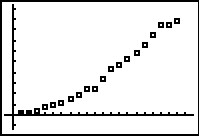
\includegraphics[width=2in]{./ExpLogsGraphics/Applications05.jpg}}

%Which models are suggested by the shape of the data?  Thinking back Section \ref{Regression}, we try a Quadratic Regression, with pretty good results.

%\begin{center}

%\begin{tabular}{cc}

%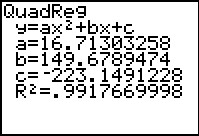
\includegraphics[width=2in]{./ExpLogsGraphics/Applications06.jpg} &

%\hspace{0.75in} 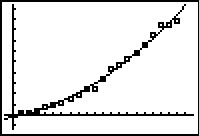
\includegraphics[width=2in]{./ExpLogsGraphics/Applications07.jpg} \\

%\end{tabular}

%\end{center}

%However, is there any scientific reason for the data to be quadratic?  Are there other models which fit the data equally well, or better?  Scientists often use logarithms in an attempt to `linearize' data sets - in other words, transform the data sets to produce ones which result in straight lines.  To see how this could work, suppose we guessed the relationship between $N$ and $t$ was some kind of power function, not necessarily quadratic, say $N = B t^{A}$.  To try to determine the $A$ and $B$, we can take the natural log of both sides and get $\ln(N) = \ln\left(B t^{A}\right)$.  Using properties of logs to expand the right hand side of this equation, we get $\ln(N) = A \ln(t) + \ln(B)$.  If we set $X = \ln(t)$ and $Y = \ln(N)$, this equation becomes $Y = AX + \ln(B)$.  In other words, we have a line with slope $A$ and $Y$-intercept $\ln(B)$.  So, instead of plotting $N$ versus $t$, we plot $\ln(N)$ versus $\ln(t)$.

%\[ \begin{array}{|c||c|c|c|c|c|c|c|c|c|c|c|c|c|}  \hline

%\ln(t) & 0 & 0.693 & 1.099 & 1.386& 1.609 & 1.792 & 1.946 & 2.079 & 2.197 & 2.302 & 2.398 & 2.485 & 2.565  \\ \hline

%\ln(N) & 4.997  & 5.549 &  5.905 & 6.489 & 6.800 & 6.989 & 7.306 & 7.546 & 7.771 & 7.824 & 8.143 & 8.385 & 8.454  \\ \hline \end{array} \]


%\[\begin{array}{|c||c||c|c|c|c|c|c|} \hline

%\ln(t) & 2.639 & 2.708 & 2.773 & 2.833 & 2.890 & 2.944 & 2.996  \\ \hline 

%\ln(N) & 8.566 & 8.653 & 8.779 & 8.925 & 9.042 & 9.045 & 9.086    \\ \hline \end{array} \]

%Running a linear regression on the data gives

%\begin{center}

%\begin{tabular}{cc}

%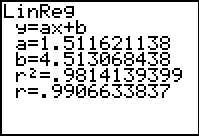
\includegraphics[width=2in]{./ExpLogsGraphics/Applications08.jpg} &

%\hspace{0.75in} 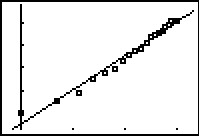
\includegraphics[width=2in]{./ExpLogsGraphics/Applications09.jpg} \\

%\end{tabular}

%\end{center}

%The slope of the regression line is $a \approx 1.512$ which corresponds to our exponent $A$.  The $y$-intercept $b \approx 4.513$ corresponds to $\ln(B)$, so that $B \approx 91.201$.  Hence, we get the model $N = 91.201 t^{1.512}$, something from Section \ref{AlgebraicFunctions}.  Of course, the calculator has a built-in `Power Regression' feature.  If we apply this to our original data set, we get the same model we arrived at before.\footnote{Critics may question why the authors of the book have chosen to even discuss linearization of data when the calculator has a Power Regression built-in and ready to go.  Our response:  talk to your science faculty.}


%\begin{center}

%\begin{tabular}{cc}

%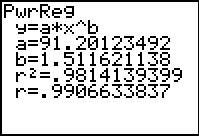
\includegraphics[width=2in]{./ExpLogsGraphics/Applications10.jpg} &

%\hspace{0.75in} 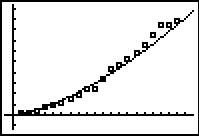
\includegraphics[width=2in]{./ExpLogsGraphics/Applications11.jpg} \\

%\end{tabular}

%\end{center}

%This is all well and good, but the quadratic model appears to fit the data better, and we've yet to mention any scientific principle which would lead us to believe the actual spread of the flu follows any kind of power function at all.  If we are to attack this data from a scientific perspective, it does seem to make sense that, at least in the early stages of the outbreak, the more people who have the flu, the faster it will spread, which leads us to proposing an uninhibited growth model. If we assume $N = B e^{At}$ then, taking logs as before, we get $\ln(N) = At + \ln(B)$.  If we set $X = t$ and $Y = \ln(N)$, then, once again, we get $Y = AX + \ln(B)$, a line with slope $A$ and $Y$-intercept $\ln(B)$.  Plotting $\ln(N)$ versus $t$ gives the following linear regression.  

%\phantomsection
%\label{swineflulinearized}

%\begin{center}

%\begin{tabular}{cc}

%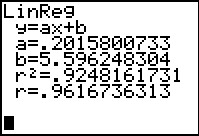
\includegraphics[width=2in]{./ExpLogsGraphics/Applications12.jpg} &

%\hspace{0.75in} 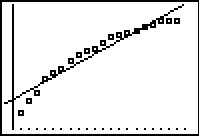
\includegraphics[width=2in]{./ExpLogsGraphics/Applications13.jpg} \\

%\end{tabular}

%\end{center}

%We see the slope is  $a \approx 0.202$ and which corresponds to $A$ in our model, and the $y$-intercept is $b \approx 5.596$ which corresponds to $\ln(B)$.  We get $B \approx 269.414$, so that our model is $N = 269.414e^{0.202t}$. Of course, the calculator has a built-in `Exponential Regression' feature which produces what appears to be a different model $N = 269.414 (1.22333419)^{t}$.  Using properties of exponents, we write $e^{0.202t} = \left(e^{0.202}\right)^t \approx (1.223848)^{t}$, which, had we carried more decimal places, would have matched the base of the calculator model exactly.

 
%\begin{center}

%\begin{tabular}{cc}

%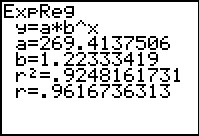
\includegraphics[width=2in]{./ExpLogsGraphics/Applications14.jpg} &

%\hspace{0.75in} 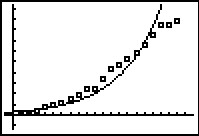
\includegraphics[width=2in]{./ExpLogsGraphics/Applications15.jpg} \\

%\end{tabular}

%\end{center}

%The exponential model didn't fit the data as well as the quadratic or power function model, but it stands to reason that, perhaps, the spread of the flu is not unlike that of the spread of a rumour and that a logistic model can be used to model the data.  The calculator does have a `Logistic Regression' feature, and using it produces the model $N = \frac{10739.147}{1 + 42.416 e^{0.268 t}}$.

%\begin{center}

%\begin{tabular}{cc}

%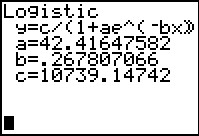
\includegraphics[width=2in]{./ExpLogsGraphics/Applications16.jpg} &

%\hspace{0.75in} 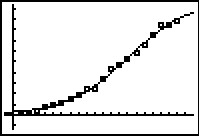
\includegraphics[width=2in]{./ExpLogsGraphics/Applications17.jpg} \\

%\end{tabular}

%\end{center}

%This appears to be an excellent fit, but there is no friendly coefficient of determination, $R^2$, by which to judge this numerically.  There are good reasons for this, but they are far beyond the scope of the text.  Which of the models, quadratic, power, exponential, or logistic is the `best model'?  If by `best' we mean `fits closest to the data,' then the quadratic and logistic models are arguably the winners with the power function model a close second.  However, if we think about the science behind the spread of the flu, the logistic model gets an edge.  For one thing, it takes into account that only a finite number of people will ever get the flu (according to our model, $10,\!739$), whereas the quadratic model predicts no limit to the number of cases. As we have stated several times before in the text, mathematical models, regardless of their sophistication, are just that:  models, and they all have their limitations.\footnote{Speaking of limitations, as of June 3, 2009, there were 19,273 confirmed cases of influenza A (H1N1).  This is well above our prediction of 10,739.  Each time a new report is issued, the data set increases and the model must be recalculated.  We leave this recalculation to the reader.}



\printexercises{exercises_pre/06_05_exercises}

\clearpage{\pagestyle{empty}\cleardoublepage}
\chapter{Foundations of Trigonometry}\label{IntroTrig}
\thispagestyle{empty}

%\section{Angles and their Measure}

\label{Angles}

This section begins our study of Trigonometry and to get started, we recall some basic definitions from Geometry.  A \index{ray ! definition of} \sword{ray} is usually described as a `half-line' and can be thought of as a line segment in which one of the two endpoints is pushed off infinitely distant from the other, as pictured in Figure \ref{fig:angles1}.  The point from which the ray originates is called the \index{ray ! initial point} \sword{initial point} of the ray.

\mfigure{.7}{A ray with initial point $P$}{fig:angles1}{figures/IntroTrigGraphics/Angles-1}


When two rays share a common initial point they form an \index{angle ! definition} \sword{angle} and the common initial point is called the \index{angle ! vertex}\index{vertex ! of an angle}\sword{vertex} of the angle.  Two  examples of what are commonly thought of as angles are given in Figure \ref{fig:angles2}

\medskip

%\addtocounter{figure}{1}
\begin{minipage}{\textwidth}
\begin{tabular}{cc}
\myincludegraphics{figures/IntroTrigGraphics/Angles-2}&
\myincludegraphics{figures/IntroTrigGraphics/Angles-3}\\
An angle with vertex $P$& An angle with vertex $Q$
\end{tabular}
\captionsetup{type=figure}
\caption{Typical angles}\label{fig:angles2}
\end{minipage}
%\addtocounter{figure}{-2}

\medskip

However, the two figures in Figure \ref{fig:angles3} also depict angles - albeit these are, in some sense, extreme cases.  In the first case, the two rays are directly opposite each other forming what is known as a \index{angle ! straight}\index{straight angle}\sword{straight angle}; in the second, the rays are identical so the `angle' is indistinguishable from the ray itself.

\medskip

%\addtocounter{figure}{2}
\begin{minipage}{\textwidth}
\begin{tabular}{cc}
\myincludegraphics{figures/IntroTrigGraphics/Angles-4} &
\myincludegraphics{figures/IntroTrigGraphics/Angles-5}\\
A straight angle &
\end{tabular}
\captionsetup{type=figure}
\caption{Less typical angles}\label{fig:angles3}
\end{minipage}
%\addtocounter{figure}{-3}

\medskip

The \index{angle ! measurement}\index{measure of an angle}\sword{measure of an angle} is a number which indicates the amount of rotation that separates the rays of the angle.  There is one immediate problem with this, as pictured in Figure \ref{fig:angles4}. 


\mtable{.45}{Two ways to measure an angle}{fig:angles4}{
\begin{tabular}{c}
\myincludegraphics{figures/IntroTrigGraphics/Angles-6}\\
\\
\myincludegraphics{figures/IntroTrigGraphics/Angles-7}\\
\end{tabular}
}


Which amount of rotation are we attempting to quantify?  What we have just discovered is that we have at least two angles described by this diagram. (The phrase `at least' will be justified in short order.)  Clearly these two angles have different measures because one appears to represent a larger rotation than the other, so we must label them differently.  In this book, we use lower case Greek letters such as $\alpha$ (alpha),   $\beta$ (beta),  $\gamma$ (gamma) and $\theta$ (theta) to label angles.  So, for instance, we have the labels in Figure \ref{fig:angles5}.

\mfigure{.2}{Labelling angles}{fig:angles5}{figures/IntroTrigGraphics/Angles-8}
\mnote{.1}{The choice of `$360$' is most often attributed to the \href{http://en.wikipedia.org/wiki/Degree_(angle)}{\underline{Babylonians}}.} 

One commonly used system to measure angles is \index{angle ! degree}\index{degree measure}\sword{degree measure}.  Quantities measured in degrees are denoted by the familiar `$^{\circ}$' symbol.  One complete revolution as shown below is $360^{\circ}$, and parts of a revolution are measured proportionately. Thus half of a revolution (a straight angle) measures $\frac{1}{2} \left(360^{\circ}\right) = 180^{\circ}$, a quarter of a revolution (a \index{right angle}\index{angle ! right}\sword{right angle}) measures $\frac{1}{4} \left(360^{\circ}\right) = 90^{\circ}$ and so on.

\medskip

\addtocounter{figure}{3}
%\ifthenelse{\isodd{\thepage}}{}{\noindent \hskip-100pt}
\noindent\begin{minipage}{\textwidth}
\begin{tabular}{ccc}
\myincludegraphics[width=0.3\textwidth]{figures/IntroTrigGraphics/Angles-9} &
\myincludegraphics[width=0.3\textwidth]{figures/IntroTrigGraphics/Angles-10} &
\myincludegraphics[width=0.3\textwidth]{figures/IntroTrigGraphics/Angles-11} \\
One revolution $\leftrightarrow 360^\circ$ & $180^\circ$ & $90^\circ$
\end{tabular}
\captionsetup{type=figure}
\caption{Defining degree measure}\label{fig:angles6}
\end{minipage}
\addtocounter{figure}{-4}

\medskip

Note that in Figure \ref{fig:angles6} above,  we have used the small square `$\! \! \! \! \! \! \qed$' to denote a right angle, as is commonplace in Geometry.  Recall that if an angle measures strictly between $0^{\circ}$ and $90^{\circ}$ it is called an \index{acute angle}\index{angle ! acute}\sword{acute angle} and if it measures strictly between $90^{\circ}$ and $180^{\circ}$ it is called an \index{obtuse angle}\index{angle ! obtuse}\sword{obtuse angle}. It is important to note that, theoretically, we can know the measure of any angle as long as we know the proportion it represents of entire revolution. For instance, the measure of an angle which represents a rotation of $\frac{2}{3}$ of a revolution would measure $\frac{2}{3} \left(360^{\circ}\right) = 240^{\circ}$,  the measure of an angle which constitutes only $\frac{1}{12}$ of a revolution measures $\frac{1}{12} \left(360^{\circ}\right) = 30^{\circ}$ and an angle which indicates no rotation at all is measured as $0^{\circ}$: see Figure \ref{fig:angles7}.

\medskip

\addtocounter{figure}{1}
%\ifthenelse{\isodd{\thepage}}{}{\noindent \hskip-100pt}
\noindent\begin{minipage}{\textwidth}
\begin{tabular}{ccc}
\myincludegraphics[width=0.3\textwidth]{figures/IntroTrigGraphics/Angles-12} &
\myincludegraphics[width=0.3\textwidth]{figures/IntroTrigGraphics/Angles-13} &
\myincludegraphics[width=0.3\textwidth]{figures/IntroTrigGraphics/Angles-14} \\
$240^\circ$ & $30^\circ$ & $0^\circ$
\end{tabular}
\captionsetup{type=figure}
\caption{Measuring angles in degrees}\label{fig:angles7}
\end{minipage}
%\addtocounter{figure}{-7}

\medskip

Two acute angles are called \index{complementary angles}\index{angle ! complementary}\sword{complementary angles} if their measures add to $90^{\circ}$.  Two angles, either a pair of right angles or one acute angle and one obtuse angle, are called \index{supplementary angles}\index{angle ! supplementary}\sword{supplementary angles} if their measures add to $180^{\circ}$. In Figure \ref{fig:angles8},  the angles $\alpha$ and $\beta$ are supplementary angles while the pair $\gamma$ and $\theta$ are complementary angles. 

\mtable{.7}{Supplementary and complementary angles}{fig:angles8}{
\begin{tabular}{c}
\myincludegraphics{figures/IntroTrigGraphics/Angles-15}\\
Supplementary angles\\
\\
\myincludegraphics{figures/IntroTrigGraphics/Angles-16}\\
Complementary angles
\end{tabular}
}


In practice, the distinction between the angle itself and its measure is blurred so that the sentence `$\alpha$ is an angle measuring $42^{\circ}$' is often abbreviated as `$\alpha = 42^{\circ}$.' 

\smallskip

Up to this point, we have discussed only angles which measure between $0^{\circ}$ and $360^{\circ}$, inclusive.  Ultimately, we want to use the arsenal of Algebra which we have stockpiled in Chapters \ref{RelationsandFunctions} through \ref{Rationals} to not only solve geometric problems involving angles, but also to extend their applicability to other real-world phenomena.  A first step in this direction is to extend our notion of `angle' from merely measuring an extent of rotation to quantities which can be associated with real numbers.  To that end, we introduce the concept of an \index{angle ! oriented}\index{oriented angle}\sword{oriented angle}.  As its name suggests, in an oriented angle, the direction of the rotation is important.  We imagine the angle being swept out starting from an \index{angle ! initial side}\index{initial side of an angle}\sword{initial side} and ending at a \index{angle ! terminal side}\index{terminal side of an angle}\sword{terminal side}, as shown in Figure \ref{fig:angles9}.  When the rotation is counter-clockwise from initial side to terminal side, we say that the angle is \index{angle ! positive}\index{positive angle}\sword{positive}; when the rotation is clockwise, we say that the angle is \index{angle ! negative}\index{negative angle}\sword{negative}.

\mtable{.4}{The sign of an angle}{fig:angles9}{
\begin{tabular}{c}
\myincludegraphics{figures/IntroTrigGraphics/Angles-17}\\
A positive angle, $45^\circ$\\
\\
\myincludegraphics{figures/IntroTrigGraphics/Angles-18}\\
A negative angle, $-45^\circ$
\end{tabular}
}

\mfigure[scale=0.9]{.2}{Angles can comprise more than one revolution}{fig:angles10}{figures/IntroTrigGraphics/Angles-19}

At this point, we also extend our allowable rotations to include angles which encompass more than one revolution.  For example, to sketch an angle with measure $450^{\circ}$ we start with an initial side, rotate counter-clockwise one complete revolution (to take care of the `first' $360^{\circ}$) then continue with an additional $90^{\circ}$ counter-clockwise rotation, as seen in Figure \ref{fig:angles10}.



To further connect angles with the Algebra which has come before, we shall often overlay an angle diagram on the coordinate plane.  An angle is said to be in \index{angle ! standard position}\index{standard position of an angle}\sword{standard position} if its vertex is the origin and its initial side coincides with the positive $x$-axis.  Angles in standard position are classified according to where their terminal side lies.  For instance, an angle in standard position whose terminal side lies in Quadrant I is called a `Quadrant I angle'.  If the terminal side of an angle lies on one of the coordinate axes, it is called a \index{angle ! quadrantal}\index{quadrantal angle}\sword{quadrantal angle}.  Two angles in standard position are called \index{angle ! coterminal}\index{coterminal angle}\sword{coterminal} if they share the same terminal side. (Note that by being in standard position they automatically share the same initial side which is the positive $x$-axis.)  In Figure \ref{fig:angles11}, $\alpha = 120^{\circ}$ and $\beta = -240^{\circ}$ are two coterminal Quadrant II angles drawn in standard position.    Note that $\alpha = \beta + 360^{\circ}$, or equivalently, $\beta = \alpha - 360^{\circ}$. We leave it as an exercise to the reader to verify that coterminal angles always differ by a multiple of $360^{\circ}$. (It is worth noting that all of the pathologies of Analytic Trigonometry result from this innocuous fact.) More precisely, if $\alpha$ and $\beta$ are coterminal angles, then $\beta = \alpha + 360^{\circ} \cdot k$ where $k$ is an integer.

%\mnote{.6}{The `quadrantal' terminology isn't something you'll encounter a lot as you move forward in your studies, so don't invest too much time in memorizing it. (On the other hand, rewriting the rest of the chapter to ignore it altogether turned out to be a bit of a challenge.) You may run into the word `coterminal' from time to time, though.}

\mfigure[scale=0.9]{.8}{Two coterminal angles, $\alpha = 120^{\circ}$ and $\beta = -240^{\circ}$, in standard position.}{fig:angles11}{figures/IntroTrigGraphics/Angles-20}

\medskip

\example{orientedcoterminaldegree}{Plotting and classifying angles}{ Graph each of the (oriented) angles below in standard position and classify them according to where their terminal side lies. Find three coterminal angles, at least one of which is positive and one of which is negative.

\begin{multicols}{2}

\begin{enumerate}

\item  $\alpha = 60^{\circ}$

\item  $\beta = -225^{\circ}$

\item  $\gamma = 540^{\circ}$

\item  $\phi = -750^{\circ}$

\end{enumerate}

\end{multicols}
}
{
\begin{enumerate}

\item  To graph $\alpha = 60^{\circ}$, we draw an angle with its initial side on the positive $x$-axis and rotate counter-clockwise $\frac{60^{\circ}}{360^{\circ}} = \frac{1}{6}$ of a revolution.  We see that $\alpha$ is a Quadrant I angle.  To find angles which are coterminal, we look for angles $\theta$ of the form $\theta = \alpha + 360^{\circ} \cdot k$, for some integer $k$.  When $k = 1$, we get $\theta =  60^{\circ} + 360^{\circ} = 420^{\circ}$.   Substituting $k = -1$ gives $\theta = 60^{\circ} - 360^{\circ} = -300^{\circ}$.  Finally, if we let $k = 2$, we get $\theta =  60^{\circ} + 720^{\circ} = 780^{\circ}$: see Figure \ref{fig:angles12}.  

\mfigure[scale=0.8]{.6}{$\alpha = 60^{\circ}$ in standard position}{fig:angles12}{figures/IntroTrigGraphics/Angles-21}

\item  Since $\beta = - 225^{\circ}$ is negative, we start at the positive $x$-axis and rotate \textit{clockwise} $\frac{225^{\circ}}{360^{\circ}} = \frac{5}{8}$ of a revolution. We see that $\beta$ is a Quadrant II angle.  To find coterminal angles, we proceed as before and compute $\theta = -225^{\circ} + 360^{\circ} \cdot k$ for integer values of $k$.  We find $135^{\circ}$, $-585^{\circ}$ and $495^{\circ}$ are all coterminal with $-225^{\circ}$: see Figure \ref{fig:angles13}.   

\mfigure[scale=0.8]{.4}{$\beta = -225^{\circ}$ in standard position}{fig:angles13}{figures/IntroTrigGraphics/Angles-22}
\mfigure[scale=0.8]{.2}{$\gamma = 540^{\circ}$ in standard position}{fig:angles14}{figures/IntroTrigGraphics/Angles-23}


\item Since $\gamma = 540^{\circ}$ is positive, we rotate counter-clockwise from the positive $x$-axis.  One full revolution accounts for $360^{\circ}$, with $180^{\circ}$, or $\frac{1}{2}$ of a revolution remaining.  Since the terminal side of $\gamma$ lies on the negative $x$-axis, $\gamma$ is a quadrantal angle.  All angles coterminal with $\gamma$ are of the form $\theta = 540^{\circ} + 360^{\circ} \cdot k$, where $k$ is an integer.  Working through the arithmetic, we find three such angles: $180^{\circ}$, $-180^{\circ}$ and $900^{\circ}$: see Figure \ref{fig:angles14}.


\item  The Greek letter $\phi$ is pronounced `fee' or `fie' and since $\phi$ is negative, we begin our rotation clockwise from the positive $x$-axis.  Two full revolutions account for $720^{\circ}$, with just $30^{\circ}$ or $\frac{1}{12}$ of a revolution to go. We find that $\phi$ is a Quadrant IV angle. To find coterminal angles, we compute $\theta = -750^{\circ} +   360^{\circ} \cdot k$ for a few integers $k$ and obtain $-390^{\circ}$, $-30^{\circ}$ and $330^{\circ}$: see Figure \ref{fig:angles15}. 


\end{enumerate}
}

\medskip

Note that since there are infinitely many integers, any given angle has infinitely many coterminal angles, and the reader is encouraged to plot the few sets of coterminal angles found in Example \ref{orientedcoterminaldegree} to see this.  We are now just one step away from completely marrying angles with the real numbers and the rest of Algebra.  To that end, we recall the following definition.

\mfigure[scale=0.8]{.82}{$\phi = -750^{\circ}$ in standard position}{fig:angles15}{figures/IntroTrigGraphics/Angles-24}

\smallskip

\definition{pidefn}{The number $\pi$}{ \index{pi, $\pi$} The real number $\pi$ is defined to be the ratio of a circle's circumference to its diameter.  In symbols, given a circle of circumference $C$ and diameter $d$, 

\[ \pi = \dfrac{C}{d} \]
}

\smallskip

While Definition \ref{pidefn} is quite possibly the `standard' definition of $\pi$, the authors would be remiss if we didn't mention that buried in this definition is actually a theorem.  As the reader is probably aware, the number $\pi$ is a mathematical constant - that is, it doesn't matter \textit{which} circle is selected, the ratio of its circumference to its diameter will have the same value as any other circle.  While this is indeed true, it is far from obvious. (If you think it \textit{is} obvious, try to come up with a rigorous proof of this fact!)   Since the diameter of a circle is twice its radius, we can quickly rearrange the equation in Definition \ref{pidefn} to get a formula more useful for our purposes, namely: $2 \pi = \dfrac{C}{r}$

This tells us that for any circle, the ratio of its circumference to its radius is also always constant; in this case the constant is $2\pi$.  Suppose now we take a \sword{portion} of the circle, so instead of comparing the entire circumference $C$ to the radius, we compare some arc measuring $s$ units in length to the radius, as depicted in Figure \ref{fig:angles16}.  Let $\theta$ be the \sword{central angle}\index{angle ! central angle}\index{central angle} subtended by this arc, that is, an angle whose vertex is the center of the circle and whose determining rays pass through the endpoints of the arc.  Using proportionality arguments, it stands to reason that the ratio $\dfrac{s}{r}$ should also be a constant among all circles, and it is this ratio which defines the \index{angle ! radian measure}\index{radian measure}\sword{radian measure} of an angle.

\mfigure[scale=0.9]{.62}{The radian measure of $\theta$ is $\dfrac{s}{r}$}{fig:angles16}{figures/IntroTrigGraphics/Angles-25}

To get a better feel for radian measure, we note that an angle with radian measure $1$ means the corresponding arc length $s$ equals the radius of the circle $r$, hence $s = r$.  When the radian measure is $2$, we have $s = 2r$; when the radian measure is $3$, $s = 3r$, and so forth.  Thus the radian measure of an angle $\theta$ tells us how many `radius lengths' we need to sweep out along the circle to subtend the angle $\theta$: see Figure \ref{fig:angles17}.

\mtable{.28}{An angle of $k$ radians subtends an arc of length $k\cdot r$}{fig:angles17}{
\begin{tabular}{c}
\myincludegraphics[scale=0.9]{figures/IntroTrigGraphics/Angles-26}\\
$\alpha$ has radian measure 1\\
\\
\myincludegraphics[scale=0.9]{figures/IntroTrigGraphics/Angles-27}\\
$\beta$ has radian measure 4
\end{tabular}}

Since one revolution sweeps out the entire circumference $2\pi r$, one revolution has radian measure $\dfrac{2 \pi r}{r} = 2 \pi$.  From this we can find the radian measure of other central angles using proportions, just like we did with degrees.    For instance, half of a revolution has radian measure  $\frac{1}{2} (2 \pi) = \pi$, a quarter revolution has radian measure $\frac{1}{4} (2 \pi) = \frac{\pi}{2}$, and so forth.   Note that, by definition, the radian measure of an angle is a length divided by another length so that these measurements are actually dimensionless and are considered `pure' numbers. For this reason, we do not use any symbols to denote radian measure, but we use the word `radians' to denote these dimensionless units as needed. For instance, we say one revolution measures `$2\pi$ radians,' half of a revolution measures `$\pi$ radians,' and so forth.  

As with degree measure, the distinction between the angle itself and its measure is often blurred in practice, so when we write  `$\theta = \frac{\pi}{2}$', we mean $\theta$ is an angle which measures $\frac{\pi}{2}$ radians. (The authors are well aware that we are now identifying radians with real numbers.  We will justify this shortly.) We extend radian measure to oriented angles, just as we did with degrees beforehand, so that a positive measure indicates counter-clockwise rotation and a negative measure indicates clockwise rotation. Much like before, two positive angles $\alpha$ and $\beta$ are supplementary if $\alpha + \beta = \pi$ and complementary if $\alpha + \beta = \frac{\pi}{2}$.   Finally, we leave it to the reader to show that when using radian measure, two angles $\alpha$ and $\beta$ are coterminal if and only if $\beta = \alpha + 2\pi k$ for some integer $k$. 

\medskip

\example{orientedcoterminalradian}{Plotting and classifying angles}{ Graph each of the (oriented) angles below in standard position and classify them according to where their terminal side lies. Find three coterminal angles, at least one of which is positive and one of which is negative.

\begin{multicols}{2}

\begin{enumerate}

\item  $\alpha = \dfrac{\pi}{6}$

\item  $\beta = -\dfrac{4\pi}{3}$

\item  $\gamma = \dfrac{9 \pi}{4}$

\item  $\phi = - \dfrac{5 \pi}{2}$

\end{enumerate}

\end{multicols}
}
{
\begin{enumerate}

\item  The angle $\alpha = \frac{\pi}{6}$ is positive, so we draw an angle with its initial side on the positive $x$-axis and rotate counter-clockwise $\frac{\left( \pi / 6\right)}{2 \pi} = \frac{1}{12}$ of a revolution.  Thus $\alpha$ is a Quadrant I angle. Coterminal angles $\theta$ are of the form $\theta = \alpha + 2\pi \cdot k$, for some integer $k$.  To make the arithmetic a bit easier, we note that $2\pi = \frac{12 \pi}{6}$, thus when $k = 1$, we get $\theta =  \frac{\pi}{6} + \frac{12 \pi}{6} = \frac{13 \pi}{6}$.   Substituting $k = -1$ gives $\theta = \frac{\pi}{6} - \frac{12 \pi}{6} = -\frac{11 \pi}{6}$ and when we let $k = 2$, we get $\theta =  \frac{\pi}{6} + \frac{24 \pi}{6} = \frac{25 \pi}{6}$: see Figure \ref{fig:angles18}.  

\mfigure[scale=0.8]{.8}{$\alpha = \frac{\pi}{6}$ in standard position.}{fig:angles18}{figures/IntroTrigGraphics/Angles-28}

\item  Since $\beta = - \frac{4\pi}{3}$ is negative, we start at the positive $x$-axis and rotate clockwise $\frac{\left(4 \pi / 3\right)}{2\pi} = \frac{2}{3}$ of a revolution.  We find $\beta$ to be a Quadrant II angle. To find coterminal angles, we proceed as before using $2\pi = \frac{6 \pi}{3}$,  and compute $\theta = -\frac{4 \pi}{3} + \frac{6 \pi}{3}  \cdot k$ for integer values of $k$.  We obtain $\frac{2\pi}{3}$, $-\frac{10 \pi}{3}$ and $\frac{8 \pi}{3}$ as coterminal angles: see Figure \ref{fig:angles19}.  

\mfigure[scale=0.8]{.6}{$\beta=-\frac{4\pi}{3}$ in standard position.}{fig:angles19}{figures/IntroTrigGraphics/Angles-29}   


\item Since $\gamma = \frac{9 \pi}{4}$ is positive, we rotate counter-clockwise from the positive $x$-axis.  One full revolution accounts for $2 \pi = \frac{8 \pi}{4}$ of the radian measure with $\frac{\pi}{4}$ or  $\frac{1}{8}$ of a revolution remaining.  We have $\gamma$ as a Quadrant I angle. All angles coterminal with $\gamma$ are of the form $\theta = \frac{9 \pi}{4} + \frac{8\pi}{4} \cdot k$, where $k$ is an integer.  Working through the arithmetic, we find: $\frac{\pi}{4}$, $-\frac{7 \pi}{4}$ and $\frac{17 \pi}{4}$: see Figure \ref{fig:angles20}.  

\mfigure[scale=0.8]{.4}{$\gamma = \frac{9\pi}{4}$ in standard position.}{fig:angles20}{figures/IntroTrigGraphics/Angles-30}

\item  To graph  $\phi = -\frac{5 \pi}{2}$, we begin our rotation clockwise from the positive $x$-axis.  As  $2 \pi = \frac{4 \pi}{2}$, after one full revolution clockwise, we have  $\frac{\pi}{2}$ or $\frac{1}{4}$ of a revolution remaining.  Since the terminal side of $\phi$ lies on the negative $y$-axis, $\phi$ is a quadrantal angle.  To find coterminal angles, we compute $\theta = -\frac{5 \pi}{2} +   \frac{4 \pi}{2} \cdot k$ for a few integers $k$ and obtain $-\frac{\pi}{2}$, $\frac{3 \pi}{2}$ and $\frac{7 \pi}{2}$: see Figure \ref{fig:angles21}.  

\mfigure[scale=0.8]{.2}{$\phi = -\frac{5\pi}{2}$ in standard position.}{fig:angles21}{figures/IntroTrigGraphics/Angles-31}

\end{enumerate}
}

\medskip

It is worth mentioning that we could have plotted the angles in Example \ref{orientedcoterminalradian} by first converting them to degree measure and following the procedure set forth in Example \ref{orientedcoterminaldegree}.  While converting back and forth from degrees and radians is certainly a good skill to have, it is best that you learn to `think in radians' as well as you can `think in degrees'.  The authors would, however, be derelict in our duties if we ignored the basic conversion between these systems altogether.  Since one revolution counter-clockwise measures $360^{\circ}$ and the same angle measures $2 \pi$ radians, we can use the proportion $\frac{2 \pi \, \text{radians}}{360^{\circ}}$, or its reduced equivalent, $\frac{\pi \, \text{radians}}{180^{\circ}}$, as the conversion factor between the two systems.  For example, to convert $60^{\circ}$ to radians we find $60^{\circ} \left( \frac{\pi \, \text{radians}}{180^{\circ}}\right) = \frac{\pi}{3} \, \text{radians}$, or simply $\frac{\pi}{3}$.  To convert from radian measure back to degrees, we multiply by the ratio $\frac{180^{\circ}}{\pi \, \text{radian}}$.  For example,  $-\frac{5 \pi}{6} \, \text{radians}$ is equal to $\left(-\frac{5 \pi}{6} \, \text{radians} \right) \left( \frac{180^{\circ}}{\pi \, \text{radians}}\right) = -150^{\circ}$.  Of particular interest is the fact that an angle which measures $1$ in radian measure is equal to $\frac{180^{\circ}}{\pi}  \approx 57.2958^{\circ}$.  

We summarize these conversions below.

\bigskip

\keyidea{degreenradianconversion}{Degree  - Radian Conversion}{

\begin{itemize}

\item  To convert degree measure to radian measure, multiply by $\dfrac{\pi \, \text{radians}}{180^{\circ}}$

\item  To convert radian measure to degree measure, multiply by $\dfrac{180^{\circ}}{\pi \, \text{radians}}$

\end{itemize}
}

\bigskip

In light of Example \ref{orientedcoterminalradian} and Equation \ref{degreenradianconversion}, the reader may well wonder what the allure of radian measure is.  The numbers involved are, admittedly, much more complicated than degree measure.  The answer lies in how easily angles in radian measure can be identified with real numbers.   Consider the Unit Circle, $x^2 + y^2 = 1$, as drawn below, the angle $\theta$ in standard position and the corresponding arc measuring $s$ units in length.  By definition, and the fact that the Unit Circle has radius 1, the radian measure of $\theta$ is $\dfrac{s}{r}=\dfrac{s}{1} = s$ so that, once again blurring the distinction between an angle and its measure, we have $\theta = s$.  In order to identify real numbers with oriented angles, we make good use of this fact by essentially  `wrapping' \index{wrapping function} the real number line around the Unit Circle and associating to each real number $t$ an \textit{oriented} arc \index{oriented arc} on the Unit Circle with initial point $(1,0)$.  This identification between angles and real numbers will also be essential once we begin our study of trigonometric functions in Calculus. 

Viewing the vertical line $x=1$ as another real number line demarcated like the $y$-axis, given a real number $t>0$, we `wrap' the (vertical) interval $[0,t]$ around the Unit Circle in a counter-clockwise fashion.  The resulting arc has a length of $t$ units and therefore the corresponding angle has radian measure equal to $t$.  If $t<0$, we wrap the interval $[t,0]$ \textit{clockwise} around the Unit Circle.  Since we have defined clockwise rotation as having negative radian measure, the angle determined by this arc has radian measure equal to $t$.    If $t=0$, we are at the point $(1,0)$ on the $x$-axis which corresponds to an angle with radian measure $0$.  In this way, we identify each real number $t$ with the corresponding angle with radian measure $t$.


\noindent\begin{minipage}{\textwidth+\marginparwidth}
\begin{tabular}{ccc}
\myincludegraphics{figures/IntroTrigGraphics/Angles-32} &
\myincludegraphics{figures/IntroTrigGraphics/Angles-33} &
\myincludegraphics{figures/IntroTrigGraphics/Angles-34} \\
On the unit circle, $\theta = s$ & Identifying $t>0$ with an angle & Identifying $t<0$ with an angle
\end{tabular}
\captionsetup{type=figure}
\caption{Identifying real numnbers with angles}\label{wrappingfunction}
\end{minipage}

\medskip

\example{realwrap}{Angles corresponding to real numbers}{  Sketch the oriented arc on the Unit Circle corresponding to each of the following real numbers.  

\begin{multicols}{2}

\begin{enumerate}

\item $t=\dfrac{3 \pi}{4}$

\item $t =  - 2 \pi$

\item $t = -2$

\item  $t = 117$

\end{enumerate}

\end{multicols}
}
{
\begin{enumerate}

\item  The arc associated with $t = \frac{3 \pi}{4}$ is the arc on the Unit Circle which subtends the angle $\frac{3 \pi}{4}$ in radian measure.  Since $\frac{3 \pi}{4}$ is $\frac{3}{8}$ of a revolution, we have an arc which begins at the point $(1,0)$ proceeds counter-clockwise up to midway through Quadrant II: see Figure \ref{fig:angles20}.  

\mfigure{.6}{$t=\frac{3\pi}{4}$}{fig:angles22}{figures/IntroTrigGraphics/Angles-35}

\item Since one revolution is $2\pi$ radians, and $t=-2\pi$ is negative, we graph  the arc which begins at $(1,0)$ and proceeds \textit{clockwise} for one full revolution: see Figure \ref{fig:angles20}.  

\mfigure{.4}{$t=-2\pi$}{fig:angles23}{figures/IntroTrigGraphics/Angles-36}

\item Like $t=-2\pi$, $t=-2$ is negative, so we begin our arc at $(1,0)$ and proceed clockwise around the unit circle.  Since $\pi \approx 3.14$ and  $\frac{\pi}{2} \approx 1.57$, we find that rotating $2$ radians clockwise from the point $(1,0)$ lands us in Quadrant III.  To more accurately place the endpoint, we successively halve the angle measure until we find $\frac{5 \pi}{8} \approx 1.96$ which tells us our arc extends just a bit beyond the quarter mark into Quadrant III: see Figure \ref{fig:angles20}.  

\mfigure{.2}{$t=-2$}{fig:angles24}{figures/IntroTrigGraphics/Angles-37}

\item  Since $117$ is positive, the arc corresponding to $t=117$ begins at $(1,0)$ and proceeds counter-clockwise.  As $117$ is much greater than $2\pi$, we wrap around the Unit Circle several times before finally reaching our endpoint.  We approximate $\frac{117}{2\pi}$ as $18.62$ which tells us we complete $18$ revolutions counter-clockwise with $0.62$, or  just shy of $\frac{5}{8}$ of a revolution to spare.  In other words, the terminal side of the angle which measures $117$ radians in standard position is just short of being midway through Quadrant III: see Figure \ref{fig:angles20}.  

\end{enumerate}
}

\medskip

\subsection{Applications of Radian Measure:  Circular Motion}
\label{circularmotion}

Now that we have paired angles with real numbers via radian measure, a whole world of applications awaits us.  Our first excursion into this realm comes by way of circular motion.  Suppose an object is moving as pictured in Figure \ref{fig:angles26} along a circular path of radius $r$ from the point $P$ to the point $Q$ in an amount of time $t$.  

\mfigure{.8}{$t=117$}{fig:angles25}{figures/IntroTrigGraphics/Angles-38} 
\mfigure{.5}{Circular motion}{fig:angles26}{figures/IntroTrigGraphics/Angles-39}

Here $s$ represents a \textit{displacement} so that  $s > 0$ means the object is travelling in a counter-clockwise direction and $s<0$ indicates movement in a clockwise direction. Note that with this convention the formula we used to define radian measure, namely $\theta = \dfrac{s}{r}$, still holds since a negative value of $s$ incurred from a clockwise displacement matches the negative we assign to $\theta$ for a clockwise rotation. 

Borrowing terminology from Physics, if we imagine the circular motion of our object taking place over a duration of time $t$, we can define the quantity $\dfrac{\theta}{t}$, called the \index{velocity ! average angular}\index{average angular velocity}\sword{average angular velocity} of the object.  It is denoted by $\overline{\omega}$ and is read `omega-bar'.  The quantity $\overline{\omega}$ is the average rate of change of the angle $\theta$ with respect to time and thus has units $\frac{\text{radians}}{\text{time}}$. If the circular motion is \textit{uniform}, meaning that the rate at which the angle $\theta$ changes with time is constant, then the average angular velocity $\overline{\omega}$ is the same as the \textit{instantaneous} angular velocity $\omega$. (If the rate is not constant, we can't define $\omega$ without calculus.)  

\smallskip

If the path of the object were `uncurled' from a circle to form a line segment, then we could discuss the average \textit{linear} velocity of the object, given by $\overline{v} = \dfrac{s}{t}$. Note that since $s = r\theta$, we obtain
\[
\overline{v} = \frac{s}{t} = \frac{r\theta}{t} = r\left(\frac{\theta}{t}\right) = r\overline{\omega}.
\]
One note of caution is needed here: the true motion of our object is, of course, \textbf{not} linear -- it's circular. Lest we draw the ire of any students with high school Physics under their belts, we should point out that motion in the plane is best described as a \textit{vector} quantity (we will \textit{not} be discussing vectors in this text), and the relationship $\overline{v} = r\overline{\omega}$ describes not the velocity of the object, but its \textit{speed}. 

\medskip

\example{EarthRotationEx}{Finding speed of rotation}{ Assuming that the surface of the Earth is a sphere, any point on the Earth can be thought of as an object travelling on a circle which completes one revolution in (approximately) 24 hours.   The path traced out by the point during this 24 hour period is the Latitude of that point.   Lakeland Community College is at $41.628^{\circ}$ north latitude, and it can be shown   that the radius of the earth at this Latitude is approximately $2960$ miles.  (We will discuss how we arrived at this approximation in Example \ref{cosinesinecircleex}.) Find the linear speed, in miles per hour, of Lakeland Community College as the world turns.
}
{  To use the formula $v = r \omega$, we first need to compute the angular velocity $\omega$.  The earth makes one revolution in 24 hours, and one revolution is $2 \pi$ radians, so $\omega = \frac{2 \pi \, \text{radians}}{24 \, \text{hours}} = \frac{\pi}{12 \, \text{hours}}$, where, once again, we are using the fact that radians are real numbers and are dimensionless. (For simplicity's sake, we are also assuming that we are viewing the rotation of the earth as counter-clockwise so $\omega > 0$.)  Hence, the linear velocity is \[ v = 2960 \, \text{miles} \cdot \frac{\pi}{12 \, \text{hours}} \approx 775 \, \frac{\text{miles}}{\text{hour}}\] }

\medskip

It is worth noting that the quantity $\frac{1 \, \text{revolution}}{24 \, \text{hours}}$ in Example \ref{EarthRotationEx} is called the \index{frequency ! ordinary} \index{ordinary frequency} \textbf{ordinary frequency} of the motion and is usually denoted by the variable $f$.  The ordinary frequency is a measure of how often an object makes a complete cycle of the motion.  The fact that $\omega = 2\pi f$ suggests that $\omega$ is also a frequency.  Indeed, it is called the \index{frequency ! angular} \index{angular frequency} \textbf{angular frequency} of the motion.  On a related note, the quantity $T = \dfrac{1}{f}$ is called the \index{period ! circular motion}\textbf{period} of the motion and is the amount of time it takes for the object to complete one cycle of the motion.  In the scenario of Example \ref{EarthRotationEx}, the period of the motion is 24 hours, or one day.  

\smallskip

The concepts of frequency and period help frame the equation $v = r \omega$ in a new light.  That is, if $\omega$ is fixed, points which are farther from the center of rotation need to travel faster to maintain the same angular frequency since they have farther to travel to make one revolution in one period's time.  The distance of the object to the center of rotation is the radius of the circle, $r$, and is the `magnification factor' which relates $\omega$ and $v$.   While we have exhaustively discussed velocities associated with circular motion, we have yet to discuss a more natural question: if an object is moving on a circular path of radius $r$ with a fixed angular velocity (frequency) $\omega$, what is the position of the object at time $t$?  The answer to this question is the very heart of Trigonometry and is answered in the next section.


\printexercises{exercises_pre/07_01_exercises}




\section{The Unit Circle: Sine and Cosine}

\label{TheUnitCircle}

In this section, we consider the problem of describing the position of a point on the unit circle.  To that end, consider an angle $\theta$ in standard position and let $P$ denote the point where the terminal side of $\theta$ intersects the Unit Circle, as in Figure \ref{fig:circle1}.  By associating the point $P$ with the angle $\theta$, we are assigning a \emph{position} on the Unit Circle to the angle $\theta$.  The $x$-coordinate of $P$ is called the \index{cosine ! of an angle} \sword{cosine} of $\theta$, written $\cos(\theta)$, while the $y$-coordinate of $P$ is called the \index{sine ! of an angle} \sword{sine} of $\theta$, written $\sin(\theta)$.  The reader is encouraged to verify that these rules used to match an angle with its cosine and sine do, in fact, satisfy the definition of a function.  That is, for each angle $\theta$, there is only one associated value of $\cos(\theta)$ and only one associated value of $\sin(\theta)$.  

\mfigure[width=0.95\marginparwidth]{.8}{Defining $\cos(\theta)$ and $\sin(\theta)$}{fig:circle1}{figures/IntroTrigGraphics/TheUnitCircle-2}
\mnote{.6}{The etymology of the name `sine' is quite colourful, and the interested reader is invited to research it;  the `co' in `cosine' is explained in Section \ref{Identities}.}



\medskip

\example{cosinesineviaunitcircle}{Evaluating $\cos(\theta)$ and $\sin(\theta)$}{  Find the cosine and sine of the following angles.

\begin{multicols}{2}

\begin{enumerate}

\item $\theta = - \pi$

\item  $\theta = \frac{\pi}{4}$

\item  $\theta = \frac{\pi}{6}$

\item  $\theta = \frac{\pi}{3}$

\end{enumerate}

\end{multicols}}
{
\begin{enumerate}

\item  The angle $\theta=-\pi$ represents one half of a clockwise revolution so its terminal side lies on the negative $x$-axis.  The point on the Unit Circle that lies on the negative $x$-axis is $(-1,0)$ which means  $\cos(-\pi) = -1$ and $\sin(-\pi) = 0$.

\mfigure[width=0.85\marginparwidth]{.2}{Finding $\cos(-\pi)$ and $\sin(-\pi)$}{fig:circle3}{figures/IntroTrigGraphics/TheUnitCircle-4}


\item  When we sketch $\theta = \frac{\pi}{4}$ in standard position, we see in Figure \ref{fig:circle4} that its terminal does not lie along any of the coordinate axes which makes our job of finding the cosine and sine values a bit more difficult. Let $P(x,y)$ denote the point on the terminal side of $\theta$ which lies on the Unit Circle. By definition,  $x = \cos\left(\frac{\pi}{4}\right)$ and $y = \sin\left(\frac{\pi}{4}\right)$.   If we drop a perpendicular line segment from $P$ to the $x$-axis, we obtain a $45^{\circ} - 45^{\circ} - 90^{\circ}$ right triangle whose legs have lengths $x$ and $y$ units. From Geometry,  we get $y=x$. (Can you show this?)  Since $P(x,y)$ lies on the Unit Circle, we have $x^2+y^2 = 1$.  Substituting $y=x$ into this equation yields $2x^2 = 1$, or $x =\pm \sqrt{\frac{1}{2}} =  \pm \frac{\sqrt{2}}{2}$.  Since $P(x,y)$ lies in the first quadrant, $x>0$, so $x = \cos\left(\frac{\pi}{4}\right) = \frac{\sqrt{2}}{2}$ and with $y=x$ we have $y = \sin\left(\frac{\pi}{4}\right) = \frac{\sqrt{2}}{2}$.  

\medskip

\noindent\hskip-20pt\begin{minipage}{\textwidth}
\begin{tabular}{m{0.6\textwidth}m{0.4\textwidth}}
\myincludegraphics[width=0.55\textwidth]{figures/IntroTrigGraphics/TheUnitCircle-5}&
\myincludegraphics[width=0.35\textwidth]{figures/IntroTrigGraphics/TheUnitCircle-6}\\
$\theta=\frac{\pi}{4}$ in standard position & $45^{\circ} - 45^{\circ} - 90^{\circ}$ triangle
\end{tabular}
\captionsetup{type=figure}
\caption{Finding $\cos\left(\frac{\pi}{4}\right)$ and $\sin\left(\frac{\pi}{4}\right)$}\label{fig:circle4}
\end{minipage}

\medskip

\item  As before, the terminal side of $\theta = \frac{\pi}{6}$ does not lie on any of the coordinate axes, so we proceed using a triangle approach.  Letting $P(x,y)$ denote the point on the terminal side of $\theta$ which lies on the Unit Circle, we drop a perpendicular line segment from $P$ to the $x$-axis to form a $30^{\circ} - 60^{\circ} - 90^{\circ}$ right triangle: see Figure \ref{fig:circle5}.  After a bit of Geometry (again, can you show this?) we find $y = \frac{1}{2}$ so $\sin\left(\frac{\pi}{6}\right) = \frac{1}{2}$.  Since $P(x,y)$ lies on the Unit Circle, we substitute $y = \frac{1}{2}$ into $x^2 + y^2 = 1$ to get $x^{2} = \frac{3}{4}$, or $x = \pm \frac{\sqrt{3}}{2}$.  Here, $x > 0$ so $x = \cos\left(\frac{\pi}{6}\right) = \frac{\sqrt{3}}{2}$.

\drawexampleline

\medskip

\noindent\hskip-20pt\begin{minipage}{\textwidth}
\begin{tabular}{m{0.5\textwidth}m{0.5\textwidth}}
\myincludegraphics[width=0.45\textwidth]{figures/IntroTrigGraphics/TheUnitCircle-7}&
\myincludegraphics[width=0.45\textwidth]{figures/IntroTrigGraphics/TheUnitCircle-8}\\
$\theta=\frac{\pi}{6}$ in standard position & $30^{\circ} - 60^{\circ} - 90^{\circ}$ triangle
\end{tabular}
\captionsetup{type=figure}
\caption{Finding $\cos\left(\frac{\pi}{6}\right)$ and $\sin\left(\frac{\pi}{6}\right)$}\label{fig:circle5}
\end{minipage}

\medskip

\item  Plotting $\theta = \frac{\pi}{3}$ in standard position, we find it is not a quadrantal angle and set about using a triangle approach. Once again, we get a   $30^{\circ} - 60^{\circ} - 90^{\circ}$ right triangle and, after the usual computations, find $x = \cos\left(\frac{\pi}{3}\right) = \frac{1}{2}$ and $y = \sin\left(\frac{\pi}{3}\right) = \frac{\sqrt{3}}{2}$.


\medskip

\noindent\hskip-20pt\begin{minipage}{\textwidth}
\begin{tabular}{m{0.65\textwidth}m{0.35\textwidth}}
\myincludegraphics[width=0.6\textwidth]{figures/IntroTrigGraphics/TheUnitCircle-9}&
\myincludegraphics[width=0.3\textwidth]{figures/IntroTrigGraphics/TheUnitCircle-10}\\
$\theta=\frac{\pi}{3}$ in standard position & $30^{\circ} - 60^{\circ} - 90^{\circ}$ triangle
\end{tabular}
\captionsetup{type=figure}
\caption{Finding $\cos\left(\frac{\pi}{3}\right)$ and $\sin\left(\frac{\pi}{3}\right)$}\label{fig:circle6}
\end{minipage}


\end{enumerate}
}

\medskip



In Example \ref{cosinesineviaunitcircle},  it was quite easy to find the cosine and sine of the quadrantal angles, but for non-quadrantal angles, the task was much more involved.   In these latter cases, we made good use of the fact that the point $P(x,y) = (\cos(\theta), \sin(\theta))$ lies on the Unit Circle, $x^2+y^2 = 1$.  If we substitute  $x=\cos(\theta)$ and $y = \sin(\theta)$ into $x^2+y^2=1$, we get  $\left(\cos(\theta)\right)^2 + \left(\sin(\theta)\right)^2 = 1$.  An unfortunate convention, which the authors are compelled to perpetuate,  is to write $\left(\cos(\theta)\right)^2$ as $\cos^{2}(\theta)$ and $\left(\sin(\theta)\right)^2$ as $\sin^{2}(\theta)$. (This is unfortunate from a `function notation' perspective, as you will see once you encounter the inverse trigonometric functions.) Rewriting the identity using this convention results in the following theorem, which is without a doubt one of the most important results in Trigonometry.

\smallskip

\theorem{cosinesinepythid}{The Pythagorean Identity}{  For any angle $\theta$, $\cos^{2}(\theta) + \sin^{2}(\theta) = 1$.
} 

\smallskip

The moniker `Pythagorean' brings to mind the Pythagorean Theorem, from which both the Distance Formula and the equation for a circle are ultimately derived.  The word `Identity' reminds us that, regardless of the angle $\theta$, the equation in Theorem \ref{cosinesinepythid} is always true.  If one of $\cos(\theta)$ or $\sin(\theta)$ is known, Theorem \ref{cosinesinepythid} can be used to determine the other, up to a ($\pm$) sign.  If, in addition, we know where the terminal side of $\theta$ lies when in standard position, then we can remove the ambiguity of the ($\pm$) and completely determine the missing value as the next example illustrates.

\medskip

\example{cosinesinepythidex}{Using the Pythagorean Identity}{ Using the given information about $\theta$, find the indicated value.

\begin{enumerate}

\item If $\theta$ is a Quadrant II angle with  $\sin(\theta) = \frac{3}{5}$, find $\cos(\theta)$.

\item If $\pi < \theta < \frac{3\pi}{2}$ with  $\cos(\theta) = -\frac{\sqrt{5}}{5}$, find $\sin(\theta)$.

\item  If $\sin(\theta) = 1$, find $\cos(\theta)$.

\end{enumerate}
}
{
\begin{enumerate} \item  When we substitute $\sin(\theta) = \frac{3}{5}$ into The Pythagorean Identity, $\cos^{2}(\theta) + \sin^{2}(\theta) = 1$, we obtain $\cos^{2}(\theta) + \frac{9}{25} = 1$.  Solving, we find $\cos(\theta) = \pm \frac{4}{5}$.  Since $\theta$ is a Quadrant II angle, its terminal side, when plotted in standard position, lies in Quadrant II.  Since the $x$-coordinates are negative in Quadrant II, $\cos(\theta)$ is too.  Hence, $\cos(\theta) = - \frac{4}{5}$.

\item Substituting $\cos(\theta) = -\frac{\sqrt{5}}{5}$ into $\cos^{2}(\theta) + \sin^{2}(\theta) = 1$ gives $\sin(\theta) = \pm \frac{2}{\sqrt{5}} = \pm \frac{2 \sqrt{5}}{5}$.  Since we are given that $\pi < \theta < \frac{3\pi}{2}$, we know $\theta$ is a Quadrant III angle. Hence both its sine and cosine are negative and we conclude $\sin(\theta) = -\frac{2 \sqrt{5}}{5}$.

\item  When we substitute $\sin(\theta) = 1$ into $\cos^{2}(\theta) + \sin^{2}(\theta) = 1$, we find $\cos(\theta) = 0$. 

\end{enumerate}
}

\medskip

Another tool which helps immensely in determining cosines and sines of angles is the symmetry inherent in the Unit Circle.  Suppose, for instance, we wish to know the cosine and sine of  $\theta = \frac{5 \pi}{6}$. We plot $\theta$ in standard position below and, as usual, let $P(x,y)$ denote the point on the terminal side of $\theta$ which lies on the Unit Circle.  Note that the terminal side of $\theta$ lies $\frac{\pi}{6}$ radians short of one half revolution.  In Example \ref{cosinesineviaunitcircle}, we determined that $\cos\left(\frac{\pi}{6}\right) = \frac{\sqrt{3}}{2}$ and $\sin\left( \frac{\pi}{6} \right) = \frac{1}{2}$.   This means that the point on the terminal side of the angle $\frac{\pi}{6}$, when plotted in standard position, is $\left(\frac{\sqrt{3}}{2}, \frac{1}{2}\right)$.  From Figure \ref{fig:circle7}, it is clear that the point $P(x,y)$ we seek can be obtained by reflecting that point about the $y$-axis.  Hence,  $\cos\left(\frac{5\pi}{6}\right) = -\frac{\sqrt{3}}{2}$ and $\sin\left( \frac{5\pi}{6} \right) = \frac{1}{2}$. 

\medskip

\noindent\begin{minipage}{0.95\textwidth}
\begin{tabular}{cc}
\myincludegraphics[width=0.45\textwidth]{figures/IntroTrigGraphics/TheUnitCircle-11}&
\myincludegraphics[width=0.45\textwidth]{figures/IntroTrigGraphics/TheUnitCircle-12}
\end{tabular}
\captionsetup{type=figure}
\caption{Refelcting $P(x,y)$ across the $y$-axis to obtain a Quadrant I angle}\label{fig:circle7}
\end{minipage}

\medskip


In the above scenario, the angle $\frac{\pi}{6}$ is called the \index{angle ! reference}\index{reference angle}\sword{reference angle} for the angle $\frac{5 \pi}{6}$. In general, for a non-quadrantal angle $\theta$, the reference angle for $\theta$ (usually denoted $\alpha$) is the \textit{acute} angle made between the terminal side of $\theta$ and the $x$-axis.  If $\theta$ is a Quadrant I or IV angle, $\alpha$ is the angle between the terminal side of $\theta$ and the \textit{positive} $x$-axis;  if $\theta$ is a Quadrant II or III angle, $\alpha$ is the angle between the terminal side of $\theta$ and the \textit{negative} $x$-axis. If we let $P$ denote the point $(\cos(\theta), \sin(\theta))$, then $P$ lies on the Unit Circle.  Since the Unit Circle possesses symmetry with respect to the $x$-axis, $y$-axis and origin, regardless of where the terminal side of $\theta$ lies, there is a point $Q$ symmetric with $P$ which determines $\theta$'s reference angle, $\alpha$ as seen below.

\mfigure[width=0.8\marginparwidth]{.8}{Reference angle $\alpha$ for a Quadrant I angle}{fig:circle8}{figures/IntroTrigGraphics/TheUnitCircle-13}
\mfigure[width=0.8\marginparwidth]{.6}{Reference angle $\alpha$ for a Quadrant II angle}{fig:circle9}{figures/IntroTrigGraphics/TheUnitCircle-14}
\mfigure[width=0.8\marginparwidth]{.4}{Reference angle $\alpha$ for a Quadrant III angle}{fig:circle10}{figures/IntroTrigGraphics/TheUnitCircle-15}
\mfigure[width=0.8\marginparwidth]{.2}{Reference angle $\alpha$ for a Quadrant IV angle}{fig:circle11}{figures/IntroTrigGraphics/TheUnitCircle-16}


We have just outlined the proof of the following theorem.

\smallskip

\theorem{refanglethm}{Reference Angle Theorem}{  Suppose $\alpha$ is the reference angle for $\theta$.  Then $\cos(\theta) = \pm \cos(\alpha)$ and $\sin(\theta) = \pm \sin(\alpha)$, where the choice of the ($\pm$) depends on the quadrant in which the terminal side of $\theta$ lies. \index{Reference Angle Theorem ! for cosine and sine}
}

\smallskip

In light of Theorem \ref{refanglethm}, it pays to know the cosine and sine values for certain common angles. In the table below, we summarize the values which we consider essential and must be memorized.

\phantomsection
\label{CosineSineFacts}

\begin{center}

\textbf{Cosine and Sine Values of Common Angles}

\vspace{-.25in}

\setlength{\extrarowheight}{4pt}

\[ \begin{array}{|c|c||c|c|} \hline
 \theta (\mbox{degrees}) &  \theta (\mbox{radians}) & \cos(\theta) & \sin(\theta) \\ \hline
0^{\circ} & 0 & 1 & 0 \\ \hline
30^{\circ} & \frac{\pi}{6} & \frac{\sqrt{3}}{2} & \frac{1}{2} \\ [2pt] \hline
45^{\circ} & \frac{\pi}{4} & \frac{\sqrt{2}}{2} & \frac{\sqrt{2}}{2} \\ [2pt] \hline
60^{\circ} & \frac{\pi}{3} & \frac{1}{2} & \frac{\sqrt{3}}{2} \\ [2pt] \hline
90^{\circ} & \frac{\pi}{2} & 0 & 1 \\ [2pt] \hline
\end{array} \]

\setlength{\extrarowheight}{0pt}

\end{center}

\medskip

\example{refangleex}{Using reference angles}{  Find the cosine and sine of the following angles.

\begin{multicols}{2}

\begin{enumerate}

\item  $\theta = \frac{5\pi}{4}$

\item  $\theta = \frac{11 \pi}{6}$

\item  $\theta = -\frac{5 \pi}{4}$

\item  $\theta = \frac{7 \pi}{3}$


\end{enumerate}

\end{multicols}
}
{
\begin{enumerate}

\item  We begin by plotting $\theta = \frac{5\pi}{4}$ in standard position and find its terminal side overshoots the negative $x$-axis to land in Quadrant III.  Hence, we obtain $\theta$'s reference angle $\alpha$ by subtracting: $\alpha = \theta - \pi = \frac{5\pi}{4} - \pi = \frac{\pi}{4}$.  Since $\theta$ is a Quadrant III angle, both $\cos(\theta) < 0$ and $\sin(\theta) < 0$.  The Reference Angle Theorem yields: $\cos\left(\frac{5\pi}{4}\right) = -\cos\left(\frac{\pi}{4}\right) = -\frac{\sqrt{2}}{2}$ and $\sin\left(\frac{5\pi}{4}\right) = - \sin\left(\frac{\pi}{4}\right) = -\frac{\sqrt{2}}{2}$.

\item The terminal side of  $\theta = \frac{11\pi}{6}$, when plotted in standard position, lies in Quadrant IV, just shy of the positive $x$-axis.  To find $\theta$'s reference angle $\alpha$, we subtract:  $\alpha = 2\pi - \theta = 2\pi - \frac{11 \pi}{6} = \frac{\pi}{6}$.  Since $\theta$ is a Quadrant IV angle, $\cos(\theta) > 0$ and $\sin(\theta) < 0$, so the Reference Angle Theorem gives: $\cos\left(\frac{11 \pi}{6} \right) = \cos\left(\frac{\pi}{6} \right) = \frac{\sqrt{3}}{2}$ and $\sin\left(\frac{11\pi}{6}\right) = -\sin\left(\frac{\pi}{6}\right) =  -\frac{1}{2}$.

\mfigure[width=0.8\marginparwidth]{.8}{Finding $\cos\left(\frac{5\pi}{4}\right)$ and $\sin\left(\frac{5\pi}{4}\right)$}{fig:circle12}{figures/IntroTrigGraphics/TheUnitCircle-17}
\mfigure[width=0.8\marginparwidth]{.6}{Finding $\cos\left(\frac{11 \pi}{6}\right)$ and  $\sin\left(\frac{11 \pi}{6}\right)$}{fig:circle13}{figures/IntroTrigGraphics/TheUnitCircle-18}
\mfigure[width=0.8\marginparwidth]{.4}{Finding $\cos\left(-\frac{5 \pi}{4}\right)$ and  $\sin\left(-\frac{5 \pi}{4}\right)$}{fig:circle14}{figures/IntroTrigGraphics/TheUnitCircle-19}


\item  To plot $\theta = -\frac{5\pi}{4}$, we rotate \textit{clockwise} an angle of $\frac{5 \pi}{4}$ from the positive $x$-axis.  The terminal side of $\theta$, therefore, lies in Quadrant II making an angle of $\alpha = \frac{5 \pi}{4} - \pi = \frac{\pi}{4}$ radians with respect to the negative $x$-axis.   Since $\theta$ is a Quadrant II angle, the Reference Angle Theorem gives:   $\cos\left(-\frac{5 \pi}{4}\right) = -\cos\left(\frac{\pi}{4}\right) = -\frac{\sqrt{2}}{2}$ and $\sin\left(-\frac{5 \pi}{4}\right) = \sin\left(\frac{\pi}{4}\right) = \frac{\sqrt{2}}{2}$. 

\item  Since the angle $\theta = \frac{7 \pi}{3}$ measures more than $2 \pi = \frac{6 \pi}{3}$, we find the terminal side of $\theta$ by rotating one full revolution followed by an additional $\alpha = \frac{7 \pi}{3} - 2\pi = \frac{\pi}{3}$ radians.  Since $\theta$ and $\alpha$ are coterminal,  $\cos\left(\frac{7\pi}{3}\right) = \cos\left(\frac{\pi}{3}\right) = \frac{1}{2}$ and $\sin\left(\frac{7\pi}{3}\right) = \sin\left(\frac{\pi}{3}\right) = \frac{\sqrt{3}}{2}$.


\mfigure[width=0.8\marginparwidth]{.2}{Finding $\cos\left(\frac{7 \pi}{3}\right)$ and  $\sin\left(\frac{7 \pi}{3}\right)$}{fig:circle15}{figures/IntroTrigGraphics/TheUnitCircle-20}



\end{enumerate}
}

\pagebreak

The reader may have noticed that when expressed in radian measure, the reference angle is easy to spot.  Reduced fraction multiples of $\pi$ with a denominator of $6$ have $\frac{\pi}{6}$ as a reference angle, those with a denominator of $4$ have $\frac{\pi}{4}$ as their reference angle, and those with a denominator of $3$ have $\frac{\pi}{3}$ as their reference angle.  The Reference Angle Theorem in conjunction with the table of cosine and sine values on Page \pageref{CosineSineFacts} can be used to generate the following figure, which the authors feel should be committed to memory. (At the very least, one should memorize the first quadrant and learn to make use of Theorem \ref{refanglethm}.)

\medskip
\noindent\hskip-110pt\begin{minipage}{\textwidth}


\index{Unit Circle ! important points}
\begin{center}
\myincludegraphics{figures/IntroTrigGraphics/TheUnitCircle-21}
\end{center}
\captionsetup{type=figure}
\caption{Important Points on the Unit Circle}\label{commonanglesunitcircle}
\end{minipage}

\pagebreak

%The next example summarizes all of the important ideas discussed thus far in the section.

%\medskip

%\example{advancedrefangleex}{Using reference angles}{  Suppose $\alpha$ is an acute angle with $\cos(\alpha) = \frac{5}{13}$.  

%\begin{enumerate}

%\item Find $\sin(\alpha)$ and use this to plot $\alpha$ in standard position.

%\item  Find the sine and cosine of the following angles:

%\begin{multicols}{2}

%\begin{enumerate}

%\item  $\theta = \pi + \alpha$

%\item  $\theta = 2\pi - \alpha$

%\item  $\theta = 3\pi - \alpha$

%\item  $\theta = \frac{\pi}{2} + \alpha$

%\end{enumerate}
%\end{multicols}

%\end{enumerate}
%}
%{
%\begin{enumerate}

%\item Proceeding as in Example \ref{cosinesinepythidex}, we substitute $\cos(\alpha) = \frac{5}{13}$ into $\cos^{2}(\alpha) + \sin^{2}(\alpha) = 1$ and find $\sin(\alpha) = \pm \frac{12}{13}$.  Since $\alpha$ is an acute (and therefore Quadrant I) angle, $\sin(\alpha)$ is positive.  Hence,  $\sin(\alpha) = \frac{12}{13}$.  To plot $\alpha$ in standard position, we begin our rotation on the positive $x$-axis to the ray which contains the point $(\cos(\alpha), \sin(\alpha)) = \left(\frac{5}{13}, \frac{12}{13}\right)$: see Figure \ref{fig:circle16}.

%\mfigure[width=0.95\marginparwidth]{.6}{Sketching $\alpha$}{fig:circle16}{figures/IntroTrigGraphics/TheUnitCircle-22}

%\item \begin{enumerate} \item To find the cosine and sine of $\theta = \pi + \alpha$, we first plot $\theta$ in standard position. We can imagine the sum of the angles $\pi + \alpha$ as a sequence of two rotations: a rotation of $\pi$ radians followed by a rotation of  $\alpha$ radians. (Since $\pi + \alpha = \alpha + \pi$, $\theta$ may be plotted by reversing the order of rotations given here. You should do this.)  We see that $\alpha$ is the reference angle for $\theta$, so by The Reference Angle Theorem,  $\cos(\theta) = \pm \cos(\alpha) = \pm \frac{5}{13}$ and $\sin(\theta) = \pm \sin(\alpha) = \pm \frac{12}{13}$. Since the terminal side of $\theta$ falls in Quadrant III, both $\cos(\theta)$ and $\sin(\theta)$ are negative, hence, $\cos(\theta) = - \frac{5}{13}$ and $\sin(\theta) = - \frac{12}{13}$.

%\medskip

%\noindent\hskip-20pt\begin{minipage}{\textwidth}
%\begin{tabular}{cc}
%\myincludegraphics[width=0.45\textwidth]{figures/IntroTrigGraphics/TheUnitCircle-23}&
%\myincludegraphics[width=0.45\textwidth]{figures/IntroTrigGraphics/TheUnitCircle-24}\\
%Visualizing $\theta = \pi+\alpha$ & $\theta$ has reference angle $\alpha$
%\end{tabular}
%\captionsetup{type=figure}
%\caption{Finding $\cos(\theta)$ and $\sin(\theta)$ in Example %\ref{advancedrefangleex}.2(a)}\label{fig:circle17}
%\end{minipage}

%\medskip



%\item  Rewriting $\theta = 2\pi - \alpha$ as $\theta = 2\pi + (-\alpha)$, we can  plot $\theta$ by visualizing one complete revolution counter-clockwise followed by a \textit{clockwise} revolution, or `backing up,'  of $\alpha$ radians.  We see that $\alpha$ is $\theta$'s reference angle, and since $\theta$ is a Quadrant IV angle, the Reference Angle Theorem gives:  $\cos(\theta) = \frac{5}{13}$ and  $\sin(\theta) = -\frac{12}{13}$.

%\medskip

%\noindent\hskip-20pt\begin{minipage}{\textwidth}
%\begin{tabular}{cc}
%\myincludegraphics[width=0.45\textwidth]{figures/IntroTrigGraphics/TheUnitCircle-25}&
%\myincludegraphics[width=0.45\textwidth]{figures/IntroTrigGraphics/TheUnitCircle-26}\\
%Visualizing $\theta = 2\pi-\alpha$ & $\theta$ has reference angle $\alpha$
%\end{tabular}
%\captionsetup{type=figure}
%\caption{Finding $\cos(\theta)$ and $\sin(\theta)$ in Example \ref{advancedrefangleex}.2(b)}\label{fig:circle18}
%\end{minipage}

%\medskip

%\drawexampleline

%\item  Taking a cue from the previous problem, we rewrite $\theta = 3\pi - \alpha$ as $\theta = 3\pi + (-\alpha)$.  The angle $3\pi$ represents one and a half revolutions counter-clockwise, so that when we `back up' $\alpha$ radians, we end up in Quadrant II.  Using the Reference Angle Theorem, we get $\cos(\theta) = -\frac{5}{13}$ and $\sin(\theta) = \frac{12}{13}$.

%\medskip

%\noindent\hskip-20pt\begin{minipage}{\textwidth}
%\begin{tabular}{cc}
%\myincludegraphics[width=0.45\textwidth]{figures/IntroTrigGraphics/TheUnitCircle-27}&
%\myincludegraphics[width=0.45\textwidth]{figures/IntroTrigGraphics/TheUnitCircle-28}\\
%Visualizing $\theta = 3\pi-\alpha$ & $\theta$ has reference angle $\alpha$
%\end{tabular}
%\captionsetup{type=figure}
%\caption{Finding $\cos(\theta)$ and $\sin(\theta)$ in Example \ref{advancedrefangleex}.2(c)}\label{fig:circle19}
%\end{minipage}

%\medskip


%\item  To plot $\theta = \frac{\pi}{2} + \alpha$, we first rotate $\frac{\pi}{2}$ radians and follow up with $\alpha$ radians.  The reference angle here is \textit{not} $\alpha$, so The Reference Angle Theorem is not immediately applicable.  (It's important that you see why this is the case.  Take a moment to think about this before reading on.)  Let $Q(x,y)$ be the point on the terminal side of $\theta$ which lies on the Unit Circle so that $x = \cos(\theta)$ and $y = \sin(\theta)$.   Once we graph $\alpha$ in standard position, we use the fact that equal angles subtend equal chords to show that the dotted lines in the figure below are equal.  Hence,  $x = \cos(\theta) = -\frac{12}{13}$.  Similarly, we find  $y = \sin(\theta) = \frac{5}{13}$. 

%\medskip

%\noindent\hskip-20pt\begin{minipage}{\textwidth}
%\begin{tabular}{cc}
%\myincludegraphics[width=0.45\textwidth]{figures/IntroTrigGraphics/TheUnitCircle-29}&
%\myincludegraphics[width=0.45\textwidth]{figures/IntroTrigGraphics/TheUnitCircle-30}\\
%Visualizing $\theta = \frac{\pi}{2}+\alpha$ & Using symmetry to determine $Q(x,y)$
%\end{tabular}
%\captionsetup{type=figure}
%\caption{Finding $\cos(\theta)$ and $\sin(\theta)$ in Example \ref{advancedrefangleex}.2(a)}\label{fig:circle20}
%\end{minipage}

%\medskip

%\end{enumerate}

%\end{enumerate}
%}

\medskip 

Our next example asks us to solve some very basic trigonometric equations.

\medskip

\example{solveforangle}{Solving basic trigonometric equations}{  Find all of the angles which satisfy the given equation.   

\begin{multicols}{3}

\begin{enumerate}

\item  \label{cosineishalf} $\cos(\theta) = \dfrac{1}{2}$

\item \label{sineisnegativehalf} $\sin(\theta) = -\dfrac{1}{2}$

\item  \label{cosineiszero} $\cos(\theta) = 0$.

\end{enumerate}

\end{multicols}}
{%Since there is no context in the problem to indicate whether to use degrees or radians, we will default to using radian measure in our answers to each of these problems.  This choice will be justified later in the text when we study what is known as Analytic Trigonometry.  In those sections to come, radian measure will be the \emph{only} appropriate angle measure so it is worth the time to become ``fluent in radians'' now.

\begin{enumerate} 

\item If $\cos(\theta) = \frac{1}{2}$, then the terminal side of $\theta$, when plotted in standard position, intersects the Unit Circle at $x = \frac{1}{2}$.  This means $\theta$ is a Quadrant I or IV angle with reference angle $\frac{\pi}{3}$.

\medskip

\noindent\hskip-10pt\begin{minipage}{\textwidth}
\begin{tabular}{cc}
\myincludegraphics[width=0.45\textwidth]{figures/IntroTrigGraphics/TheUnitCircle-31}&
\myincludegraphics[width=0.45\textwidth]{figures/IntroTrigGraphics/TheUnitCircle-32}\\
\end{tabular}
\captionsetup{type=figure}
\caption{Angles with $\cos(\theta)=\frac{1}{2}$}\label{fig:circle21}
\end{minipage}


One solution in  Quadrant I is  $\theta = \frac{\pi}{3}$, and since all other Quadrant I solutions must be coterminal with $\frac{\pi}{3}$, we find $\theta = \frac{\pi}{3} + 2\pi k$ for integers $k$.  Proceeding similarly for the Quadrant IV case, we find the solution to $\cos(\theta) = \frac{1}{2}$ here is $\frac{5 \pi}{3}$, so our answer in this Quadrant  is $\theta = \frac{5\pi}{3} + 2\pi k$ for integers $k$. 

%\mnote{.85}{Recall from Section \ref{Angles} that two angles in radian measure are coterminal if and only if they differ by an integer multiple of $2\pi$.  Hence to describe all angles coterminal with a given angle, we add $2\pi k$ for integers $k = 0$, $\pm 1$, $\pm 2$, \dots.}

\item  If $\sin(\theta) = -\frac{1}{2}$, then when $\theta$ is plotted in standard position, its terminal side intersects the Unit Circle at  $y=-\frac{1}{2}$.  From this, we determine $\theta$ is a Quadrant III or Quadrant IV angle with reference angle $\frac{\pi}{6}$.


\medskip

\noindent\hskip-10pt\begin{minipage}{\textwidth}
\begin{tabular}{cc}
\myincludegraphics[width=0.45\textwidth]{figures/IntroTrigGraphics/TheUnitCircle-33}&
\myincludegraphics[width=0.45\textwidth]{figures/IntroTrigGraphics/TheUnitCircle-34}\\
\end{tabular}
\captionsetup{type=figure}
\caption{Angles with $\sin(\theta)=-\frac{1}{2}$}\label{fig:circle22}
\end{minipage}

\medskip

In Quadrant III, one solution is $\frac{7\pi}{6}$, so we capture all Quadrant III solutions by adding integer multiples of $2\pi$:  $\theta = \frac{7\pi}{6} + 2\pi k$. In Quadrant IV, one solution is $\frac{11\pi}{6}$ so all the solutions here are of the form $\theta = \frac{11\pi}{6} + 2\pi k$ for integers $k$.

\item  The angles with $\cos(\theta) = 0$ are quadrantal angles whose terminal sides, when plotted in standard position, lie along the $y$-axis.   


\medskip

\noindent\hskip-10pt\begin{minipage}{\textwidth}
\begin{tabular}{cc}
\myincludegraphics[width=0.45\textwidth]{figures/IntroTrigGraphics/TheUnitCircle-35}&
\myincludegraphics[width=0.45\textwidth]{figures/IntroTrigGraphics/TheUnitCircle-36}\\
\end{tabular}
\captionsetup{type=figure}
\caption{Angles with $\cos(\theta)=0$}\label{fig:circle23}
\end{minipage}

\medskip

While, technically speaking, $\frac{\pi}{2}$ isn't a reference angle we can nonetheless use it to find our answers.  If we follow the procedure set forth in the previous examples, we find $\theta = \frac{\pi}{2} + 2\pi k$ and $\theta = \frac{3\pi}{2} + 2\pi k$ for integers, $k$. While this solution is correct, it can be shortened to $\theta = \frac{\pi}{2} + \pi k$ for integers $k$.  (Can you see why this works from the diagram?)

\end{enumerate}
}

\medskip

One of the key items to take from Example \ref{solveforangle} is that, in general, solutions to trigonometric equations consist of infinitely many answers.  The reader is encouraged write out as many of these answers as necessary to get a feel for them.   This is especially important when checking answers to the exercises.   For example, another Quadrant IV solution to $\sin(\theta) = -\frac{1}{2}$ is $\theta = -\frac{\pi}{6}$.  Hence, the family of Quadrant IV answers to number \ref{sineisnegativehalf} above could just have easily been written $\theta = -\frac{\pi}{6} + 2\pi k$ for integers $k$.  While on the surface, this family may look different than the stated solution of $\theta = \frac{11\pi}{6} + 2\pi k$ for integers $k$, we leave it to the reader to show they represent the same list of angles.



\medskip

We close this section by noting that we can easily extend the functions cosine and sine to real numbers by identifying a real number $t$ with the angle $\theta = t$ radians.  Using this identification, we define $\cos(t) = \cos(\theta)$ and $\sin(t) = \sin(\theta)$. In practice this means expressions like $\cos(\pi)$ and $\sin(2)$ can be found by regarding the inputs as angles in radian measure or real numbers;  the choice is the reader's.  


In the same way we studied polynomial, rational, exponential, and logarithmic functions, we will study the trigonometric functions $f(t) = \cos(t)$ and $g(t) = \sin(t)$.  The first order of business is to find the domains and ranges of these functions.  Whether we think of identifying the real number $t$ with the angle $\theta = t$ radians, or think of wrapping an oriented arc around the Unit Circle to find coordinates on the Unit Circle, it should be clear that both the cosine and sine functions are defined for all real numbers $t$.  In other words, the domain  of $f(t) = \cos(t)$ and of $g(t) = \sin(t)$ is $(-\infty, \infty)$.  Since $\cos(t)$ and $\sin(t)$ represent $x$- and $y$-coordinates, respectively, of points on the Unit Circle, they both take on all of the values between $-1$ an $1$, inclusive.  In other words, the range of $f(t) = \cos(t)$ and of $g(t) = \sin(t)$ is the interval $[-1,1]$.  To summarize:

\mtable{.65}{Defining $\cos(t)$ and $\sin(t)$ as functions of a real variable}{fig:circle28}{
\begin{tabular}{c}
\myincludegraphics[width=0.95\marginparwidth]{figures/IntroTrigGraphics/TheUnitCircle-46}\\
\\
\myincludegraphics[width=0.95\marginparwidth]{figures/IntroTrigGraphics/TheUnitCircle-47}
\end{tabular}
}

\smallskip

\theorem{cosinesinefunctiondomainrange}{Domain and Range of the Cosine and Sine Functions}{
\begin{multicols}{2}
\begin{itemize}
\item The function $f(t)=\cos(t)$
\begin{itemize}
\item has domain $(-\infty,\infty)$
\item has range $[-1,1]$
\end{itemize}
\item The function $g(t)=\sin(t)$
\begin{itemize}
\item has domain $(-\infty,\infty)$
\item has range $[-1,1]$
\end{itemize}
\end{itemize}
\end{multicols}
}

\smallskip
\phantomsection
\label{cosinesineequationsrealnumbers}

Suppose, as in the Exercises, we are asked to solve an equation such as $\sin(t) = -\frac{1}{2}$.  As we have already mentioned, the distinction between $t$ as a real number and as an angle $\theta = t$ radians is often blurred. Indeed, we solve $\sin(t) = -\frac{1}{2}$ in the exact same manner as we did in Example \ref{solveforangle} number \ref{sineisnegativehalf}.  Our solution is only cosmetically different in that the variable used is $t$ rather than $\theta$:  $t = \frac{7\pi}{6} + 2\pi k$ or  $t = \frac{11\pi}{6} + 2\pi k$ for integers, $k$.  We will study the cosine and sine functions in greater detail in Section \ref{TrigGraphs}.  Until then, keep in mind that any properties of cosine and sine developed in the following sections which regard them as functions of \textit{angles} in \textit{radian} measure apply equally well if the inputs are regarded as \textit{real numbers}.

\printexercises{exercises_pre/07_02_exercises}

\section{The Six Circular Functions and Fundamental Identities}

\label{CircularFunctions}

In section \ref{TheUnitCircle},  we defined $\cos(\theta)$ and $\sin(\theta)$  for angles $\theta$ using the coordinate values of points on the Unit Circle.  As such, these functions earn the moniker \index{circular function}\index{function ! circular}\textbf{circular functions}. It turns out that cosine and sine are just two of the six commonly used circular functions which we define below. 

\mnote{.7}{The functions in Definition \ref{circularfunctions} are also (and perhaps, more commonly) known as \textit{trigonometric} functions, owing to the fact that the can also be defined in terms of ratios of the three sides of a right-angle triangle}

%\enlargethispage{.2in}

\smallskip

\definition{circularfunctions}{The Circular Functions}{ Suppose $\theta$ is an angle plotted in standard position and $P(x,y)$ is the point on the terminal side of $\theta$ which lies on the Unit Circle.  

\begin{itemize}

\item The \index{cosine ! of an angle} \sword{cosine} of $\theta$, denoted $\cos(\theta)$, is defined by $\cos(\theta) = x$.

\item The \index{sine ! of an angle} \sword{sine} of $\theta$, denoted $\sin(\theta)$, is defined by $\sin(\theta) = y$.

\item The \index{secant ! of an angle} \sword{secant} of $\theta$, denoted $\sec(\theta)$, is defined by $\sec(\theta) = \dfrac{1}{x}$, provided $x \neq 0$.

\item The \index{cosecant ! of an angle} \sword{cosecant} of $\theta$, denoted $\csc(\theta)$, is defined by $\csc(\theta) = \dfrac{1}{y}$, provided $y \neq 0$.

\item The \index{tangent ! of an angle} \sword{tangent} of $\theta$, denoted $\tan(\theta)$, is defined by $\tan(\theta) = \dfrac{y}{x}$, provided $x \neq 0$.

\item The \index{cotangent ! of an angle} \sword{cotangent} of $\theta$, denoted $\cot(\theta)$, is defined by $\cot(\theta) = \dfrac{x}{y}$, provided $y \neq 0$.

\end{itemize}
}

\smallskip

While we left the history of the name `sine' as an interesting research project in Section \ref{TheUnitCircle}, the names `tangent' and `secant' can be explained using the diagram below.  Consider the acute angle $\theta$ below in standard position. Let $P(x,y)$ denote, as usual,  the point on the terminal side of $\theta$ which lies on the Unit Circle and let $Q(1,y')$ denote the point on the terminal side of $\theta$ which lies on the vertical line $x=1$, as in Figure \ref{fig:cirfun1}. 

\mfigure[width=0.95\marginparwidth]{.4}{Explaining the tangent and secant functions}{fig:cirfun1}{figures/IntroTrigGraphics/CircularFunctions-1}

%\medskip

The word `tangent' comes from the Latin meaning `to touch,' and for this reason, the line $x=1$ is called a \textit{tangent} line to the Unit Circle since it intersects, or `touches', the circle at only one point, namely $(1,0)$.  Dropping perpendiculars from $P$ and $Q$ creates a pair of similar triangles $\Delta OPA$ and $\Delta OQB$.  Thus $\frac{y'}{y} = \frac{1}{x}$ which gives  $y' = \frac{y}{x} = \tan(\theta)$, where this last equality comes from applying Definition  \ref{circularfunctions}. We have just shown that for acute angles $\theta$, $\tan(\theta)$ is the $y$-coordinate of the point on the terminal side of $\theta$ which lies on the line $x = 1$ which is \textit{tangent} to the Unit Circle. Now the word `secant' means `to cut', so a secant line is any line that `cuts through' a circle at two points. (Compare this with the definition given in Section \ref{LinearFunctions}.)  The line containing the terminal side of $\theta$ is a secant line since it intersects the Unit Circle in Quadrants I and III.   With the point $P$ lying on the Unit Circle, the length of the hypotenuse of $\Delta OPA$ is $1$. If we let $h$ denote the length of the hypotenuse of $\Delta OQB$, we have from similar triangles that $\frac{h}{1} = \frac{1}{x}$, or $h = \frac{1}{x} = \sec(\theta)$.  Hence for an acute angle $\theta$, $\sec(\theta)$ is the length of the line segment which lies on the secant line determined by the terminal side of $\theta$ and `cuts off' the tangent line $x=1$.  Not only do these observations help explain the names of these functions, they serve as the basis for a fundamental inequality needed for Calculus which we'll explore in the Exercises.

\smallskip 

Of the six circular functions, only cosine and sine are defined for all angles.  Since $\cos(\theta) = x$ and $\sin(\theta) = y$ in Definition \ref{circularfunctions}, it is customary to rephrase the remaining four circular functions in terms of cosine and sine.  The following theorem is a result of simply replacing $x$ with $\cos(\theta)$ and $y$ with $\sin(\theta)$ in Definition \ref{circularfunctions}.

\smallskip

\theorem{recipquotid}{Reciprocal and Quotient Identities}{ \index{Reciprocal Identities} \index{Quotient Identities} 

\begin{itemize}

\item $\sec(\theta) = \dfrac{1}{\cos(\theta)}$, provided $\cos(\theta) \neq 0$;  if $\cos(\theta) = 0$, $\sec(\theta)$ is undefined.

\item $\csc(\theta) = \dfrac{1}{\sin(\theta)}$, provided $\sin(\theta) \neq 0$;  if $\sin(\theta) = 0$, $\csc(\theta)$ is undefined.

\item $\tan(\theta) = \dfrac{\sin(\theta)}{\cos(\theta)}$, provided $\cos(\theta) \neq 0$;  if $\cos(\theta) = 0$, $\tan(\theta)$ is undefined.

\item $\cot(\theta) = \dfrac{\cos(\theta)}{\sin(\theta)}$, provided $\sin(\theta) \neq 0$;  if $\sin(\theta) = 0$, $\cot(\theta)$ is undefined.

\end{itemize}
}

\medskip

\example{circularfunctionsex}{Evaluating circular functions}{  Find the indicated value, if it exists.

\begin{enumerate}

\item  $\csc\left(\frac{7 \pi}{4} \right)$

\item  $\cot(3)$

\item $\tan\left(\theta\right)$, where $\theta$ is any angle coterminal with $\frac{3\pi}{2}$.

\item $\cos\left(\theta\right)$, where $\csc(\theta) = -\sqrt{5}$ and $\theta$ is a Quadrant IV angle.

\item $\sin\left(\theta\right)$, where $\tan(\theta) = 3$ and $\pi < \theta < \frac{3\pi}{2}$.

\end{enumerate}}
{
\begin{enumerate}

\item  Since $\sin\left( \frac{7\pi}{4}\right) = - \frac{\sqrt{2}}{2}$,  $\csc\left( \frac{7\pi}{4}\right) = \frac{1}{\sin\left( \frac{7\pi}{4}\right)} = \frac{1}{- \sqrt{2}/2} = - \frac{2}{\sqrt{2}} = - \sqrt{2}$.

\item  Since $\theta = 3$ radians is not one of the `common angles' from Section \ref{TheUnitCircle}, we resort to the calculator for a decimal approximation.  Ensuring that the calculator is in radian mode, we find $\cot(3) = \frac{\cos(3)}{\sin(3)} \approx -7.015$.

\item  If $\theta$ is coterminal with $\frac{3 \pi}{2}$, then $\cos(\theta) = \cos\left(\frac{3 \pi}{2}\right) = 0$ and $\sin(\theta) = \sin\left(\frac{3 \pi}{2}\right) = -1$.  Attempting to compute $\tan(\theta) = \frac{\sin(\theta)}{\cos(\theta)}$ results in $\frac{-1}{0}$, so $\tan(\theta)$ is undefined.

\item  We are given that $\csc(\theta) = \frac{1}{\sin(\theta)} = -\sqrt{5}$ so $\sin(\theta) = -\frac{1}{\sqrt{5}} = -\frac{\sqrt{5}}{5}$.  As we saw in Section \ref{TheUnitCircle}, we can use the Pythagorean Identity, $\cos^{2}(\theta) + \sin^2(\theta) = 1$, to find $\cos(\theta)$ by knowing $\sin(\theta)$.  Substituting, we get $\cos^{2}(\theta) + \left(-\frac{\sqrt{5}}{5}\right)^2 = 1$, which gives $\cos^{2}(\theta) = \frac{4}{5}$, or $\cos(\theta) = \pm \frac{2 \sqrt{5}}{5}$.  Since $\theta$ is a Quadrant IV angle, $\cos(\theta) > 0$, so $\cos(\theta) = \frac{2 \sqrt{5}}{5}$.

\item \label{commontanmistake} If $\tan(\theta) = 3$, then $\frac{\sin(\theta)}{\cos(\theta)} = 3$.  Be careful - this does \textbf{NOT} mean we can take $\sin(\theta) = 3$ and $\cos(\theta) = 1$. Instead, from $\frac{\sin(\theta)}{\cos(\theta)} = 3$  we get: $\sin(\theta) = 3 \cos(\theta)$.  To relate $\cos(\theta)$ and $\sin(\theta)$, we once again employ the Pythagorean Identity, $\cos^{2}(\theta) + \sin^{2}(\theta) = 1$.  Solving $\sin(\theta) = 3 \cos(\theta)$ for $\cos(\theta)$, we find $\cos(\theta) = \frac{1}{3} \sin(\theta)$.  Substituting this into the Pythagorean Identity, we find  $\sin^{2}(\theta) + \left(\frac{1}{3} \sin(\theta)\right)^2 = 1$. Solving, we get $\sin^{2}(\theta) = \frac{9}{10}$ so $\sin(\theta) = \pm \frac{3 \sqrt{10}}{10}$.  Since $\pi < \theta < \frac{3\pi}{2}$, $\theta$ is  a Quadrant III angle.  This means $\sin(\theta) < 0$, so our final answer is  $\sin(\theta) = - \frac{3 \sqrt{10}}{10}$.

\end{enumerate}
}

\medskip

%While the Reciprocal and Quotient Identities presented in Theorem \ref{recipquotid} allow us to always reduce problems involving secant, cosecant, tangent and cotangent to problems involving cosine and sine, it is not always convenient to do so.  It is worth taking the time to memorize the tangent and cotangent values of the common angles summarized below.

%\mnote{.5}{As we shall see shortly, when solving equations involving secant and cosecant, we usually convert back to cosines and sines.  However, when solving for tangent or cotangent, we usually stick with what we're dealt.}

%\begin{center}

%\textbf{Tangent and Cotangent Values of Common Angles}

%\vspace{-.25in}

%\setlength{\extrarowheight}{4pt}

%\[ \begin{array}{|c|c||c|c|} \hline
% \theta (\mbox{degrees}) &  \theta (\mbox{radians}) & \tan(\theta) & \cot(\theta) \\ \hline
%0^{\circ} & 0 & 0 & \text{undefined} \\ \hline
%30^{\circ} & \frac{\pi}{6} & \frac{\sqrt{3}}{3} & \sqrt{3} \\ [2pt] \hline
%45^{\circ} & \frac{\pi}{4} & 1 & 1 \\ [2pt] \hline
%60^{\circ} & \frac{\pi}{3} & \sqrt{3} & \frac{\sqrt{3}}{3} \\ [2pt] \hline
%90^{\circ} & \frac{\pi}{2} & \text{undefined} & 0 \\ [2pt] \hline
%\end{array} \]

%\setlength{\extrarowheight}{0pt}

%\end{center}

%Coupling Theorem \ref{recipquotid} with the Reference Angle Theorem, Theorem \ref{refanglethm}, we get the following.

%\smallskip

%\theorem{genrefanglethm}{Generalized Reference Angle Theorem}{  The values of the circular functions of an angle, if they exist, are the same, up to a sign, of the corresponding circular functions of its reference angle.  More specifically, if $\alpha$ is the reference angle for $\theta$,  then: $\cos(\theta)  = \pm \cos(\alpha)$, $\sin(\theta)  = \pm \sin(\alpha)$, $\sec(\theta)  = \pm \sec(\alpha)$, $\csc(\theta)  = \pm \csc(\alpha)$, $\tan(\theta)  = \pm \tan(\alpha)$ and $\cot(\theta)  = \pm \cot(\alpha)$.  The choice of the ($\pm$) depends on the quadrant in which the terminal side of $\theta$ lies. \index{Reference Angle Theorem ! for the circular functions}
%}

%\smallskip

%We put Theorem \ref{genrefanglethm} to good use in the following example.

%\pagebreak

%\example{solveforangle2}{Solving basic trigonometric equations}{  Find all angles which satisfy the given equation.   

%\begin{multicols}{3}

%\begin{enumerate}

%\item  $\sec(\theta) =2$

%\item  $\tan(\theta) = \sqrt{3}$

%\item  \label{cotangentisnegativeone} $\cot(\theta) = -1$.

%\end{enumerate}

%\end{multicols}}
%{
%\begin{enumerate}

%\item  To solve $\sec(\theta) = 2$, we convert to cosines and get $\frac{1}{\cos(\theta)} = 2$ or $\cos(\theta) = \frac{1}{2}$.  This is the exact same equation we solved in Example \ref{solveforangle}, number \ref{cosineishalf}, so we know the answer is:  $\theta = \frac{\pi}{3} + 2\pi k$ or $\theta = \frac{5\pi}{3} + 2\pi k$ for integers $k$.

%\item From the table of common values, we see  $\tan\left(\frac{\pi}{3}\right) = \sqrt{3}$.  According to Theorem \ref{genrefanglethm}, we  know  the solutions to $\tan(\theta) = \sqrt{3}$ must, therefore, have a reference angle of $\frac{\pi}{3}$. Our next task is to determine in which quadrants the solutions to this equation lie. Since tangent is defined as the ratio $\frac{y}{x}$ of points $(x,y)$ on the Unit Circle with $x \neq 0$, tangent is positive when $x$ and $y$ have the same sign (i.e., when they are both positive or both negative.)  This happens in Quadrants I and III.  In Quadrant I, we get the solutions: $\theta = \frac{\pi}{3} + 2\pi k$ for integers $k$, and for Quadrant III, we get $\theta = \frac{4\pi}{3} + 2\pi k$ for integers $k$.  While these descriptions of the solutions are correct, they can be combined into one list as $\theta = \frac{\pi}{3} + \pi k$ for integers $k$. The latter form of the solution is best understood looking at the geometry of the situation in Figure \ref{fig:cirfun2}. (See Example \ref{solveforangle} number \ref{cosineiszero} in Section \ref{TheUnitCircle} for another example of this kind of simplification of the solution.)
 
%\mtable{.7}{Solving $\tan(\theta)=\sqrt{3}$}{fig:cirfun2}{
%\begin{tabular}{c}
% \myincludegraphics[width=0.95\marginparwidth]{figures/IntroTrigGraphics/CircularFunctions-2}\\
% \\
% \myincludegraphics[width=0.95\marginparwidth]{figures/IntroTrigGraphics/CircularFunctions-3} 
%\end{tabular}}
  

%\item  From the table of common values, we see that $\frac{\pi}{4}$ has a cotangent of $1$, which means the solutions to $\cot(\theta) = -1$ have a reference angle of $\frac{\pi}{4}$. To find the quadrants in which our solutions lie, we note that $\cot(\theta) = \frac{x}{y}$ for a point $(x,y)$ on the Unit Circle where $y \neq 0$. If $\cot(\theta)$ is negative, then $x$ and $y$ must have different signs (i.e., one positive and one negative.)  Hence, our solutions lie in Quadrants II and IV: see Figure \ref{fig:cirfun3}.  Our Quadrant II solution is $\theta = \frac{3\pi}{4} + 2\pi k$, and for Quadrant IV, we get $\theta = \frac{7\pi}{4} + 2\pi k$ for integers $k$.  Can these lists be combined?  Indeed they can - one such way to capture all the solutions is:  $\theta = \frac{3\pi}{4} + \pi k$ for integers $k$.

%\mtable{.28}{Solving $\cot(\theta)=-1$}{fig:cirfun3}{
%\begin{tabular}{c}
% \myincludegraphics[width=0.95\marginparwidth]{figures/IntroTrigGraphics/CircularFunctions-4}\\
% \\
% \myincludegraphics[width=0.95\marginparwidth]{figures/IntroTrigGraphics/CircularFunctions-5} 
%\end{tabular}}

%\end{enumerate}
%}

%\medskip

Our next step is to provide versions of the identity $\cos^2(\theta)+\sin^2(\theta)=1$ for the remaining circular functions.   Assuming $\cos(\theta) \neq 0$, we may start with $\cos^{2}(\theta) + \sin^{2}(\theta) = 1$ and divide both sides by $\cos^{2}(\theta)$ to obtain $1 + \frac{\sin^{2}(\theta)}{\cos^{2}(\theta)} = \frac{1}{\cos^{2}(\theta)}$.  Using properties of exponents along with the Reciprocal and Quotient Identities, this reduces to $1 + \tan^{2}(\theta) = \sec^{2}(\theta)$.  If $\sin(\theta) \neq 0$, we can divide both sides of the identity $\cos^{2}(\theta) + \sin^{2}(\theta) = 1$ by $\sin^{2}(\theta)$, apply Theorem \ref{recipquotid} once again,  and obtain $\cot^{2}(\theta) + 1 = \csc^{2}(\theta)$.  These three Pythagorean Identities are worth memorizing and they, along with some of their other common forms, are summarized in the following theorem.

\smallskip

\theorem{pythids}{The Pythagorean Identities}{ \index{Pythagorean Identities}

\begin{enumerate}

\item $\cos^{2}(\theta) + \sin^{2}(\theta) = 1$.

\textbf{Common Alternate Forms:}

\begin{itemize}

\item  $1 - \sin^{2}(\theta) = \cos^{2}(\theta)$

\item  $1 - \cos^{2}(\theta) = \sin^{2}(\theta)$

\end{itemize}

\item $1 + \tan^{2}(\theta) = \sec^{2}(\theta)$, provided $\cos(\theta) \neq 0$.

\textbf{Common Alternate Forms:}

\begin{itemize}

\item  $\sec^{2}(\theta) - \tan^{2}(\theta) = 1$

\item  $\sec^{2}(\theta) - 1 = \tan^{2}(\theta)$

\end{itemize}

\item $1 + \cot^{2}(\theta) = \csc^{2}(\theta)$, provided $\sin(\theta) \neq 0$.

\textbf{Common Alternate Forms:}

\begin{itemize}

\item  $\csc^{2}(\theta) - \cot^{2}(\theta) = 1$

\item  $\csc^{2}(\theta) - 1 = \cot^{2}(\theta)$

\end{itemize}

\end{enumerate}
}

%\smallskip

%Trigonometric identities play an important role in not just Trigonometry, but in Calculus as well.  We'll use them in this book to find the values of the circular functions of an angle and solve equations and inequalities.  In Calculus, they are needed to simplify otherwise complicated expressions.  In the next example, we make good use of the Theorems \ref{recipquotid} and \ref{pythids}.

\pagebreak

\example{idornotex1}{Verifying trigonometric identities}{ Verify the following identities. Assume that all quantities are defined.

\begin{multicols}{2}

\begin{enumerate}

\item  $\dfrac{1}{\csc(\theta)} = \sin(\theta)$

\item  $\tan(\theta) = \sin(\theta) \sec(\theta)$ 

\setcounter{HW}{\value{enumi}}

\end{enumerate}

\end{multicols}

\begin{multicols}{2}

\begin{enumerate}

\setcounter{enumi}{\value{HW}}

\item  $(\sec(\theta) - \tan(\theta)) (\sec(\theta) + \tan(\theta)) = 1$ 

\item  $\dfrac{\sec(\theta)}{1 - \tan(\theta)} = \dfrac{1}{\cos(\theta) - \sin(\theta)}$

\setcounter{HW}{\value{enumi}}

\end{enumerate}

\end{multicols}

%\begin{multicols}{2}

%\begin{enumerate}

%\setcounter{enumi}{\value{HW}}

%\item  $6\sec(\theta) \tan(\theta) = \dfrac{3}{1-\sin(\theta)} - \dfrac{3}{1 + \sin(\theta)}$

%\item  \label{pythconjex} $\dfrac{\sin(\theta)}{1 - \cos(\theta)} = \dfrac{1 + \cos(\theta)}{\sin(\theta)}$

%\end{enumerate}

%\end{multicols}
}
{In verifying identities, we typically start with the more complicated side of the equation and use known identities to \textit{transform} it into the other side of the equation. 

\begin{enumerate} 

\item  To verify $\frac{1}{\csc(\theta)} = \sin(\theta)$, we start with the left side.  Using $\csc(\theta) = \frac{1}{\sin(\theta)}$, we get:  \[ \dfrac{1}{\csc(\theta)} = \dfrac{1}{\frac{1}{\sin(\theta)}} = \sin(\theta),\]

%\enlargethispage{.1in} 
which is what we were trying to prove.

\item Starting with the right hand side of $\tan(\theta) = \sin(\theta) \sec(\theta)$, we use $\sec(\theta) = \frac{1}{\cos(\theta)}$ and find:  \[ \sin(\theta) \sec(\theta) = \sin(\theta) \dfrac{1}{\cos(\theta)} = \dfrac{\sin(\theta)}{\cos(\theta)} = \tan(\theta),\]

where the last equality is courtesy of Theorem \ref{recipquotid}.

\item Expanding the left hand side of the equation gives:  $(\sec(\theta) - \tan(\theta)) (\sec(\theta) + \tan(\theta)) = \sec^{2}(\theta) - \tan^{2}(\theta)$.  According to Theorem \ref{pythids}, $\sec^{2}(\theta) - \tan^{2}(\theta) = 1$.  Putting it all together, \[(\sec(\theta) - \tan(\theta)) (\sec(\theta) + \tan(\theta)) = \sec^{2}(\theta) - \tan^{2}(\theta)  = 1.\]

\enlargethispage{1.5\baselineskip}

\item  While both sides of our last identity contain fractions, the left side affords us more opportunities to use our identities.  Substituting $\sec(\theta) = \frac{1}{\cos(\theta)}$ and $\tan(\theta) = \frac{\sin(\theta)}{\cos(\theta)}$, we get:


\[ \begin{array}{rcl} \dfrac{\sec(\theta)}{1 - \tan(\theta)} & = & \dfrac{ \dfrac{1}{\cos(\theta)}}{1 - \dfrac{\sin(\theta)}{\cos(\theta)}} = \dfrac{ \dfrac{1}{\cos(\theta)}}{1 - \dfrac{\sin(\theta)}{\cos(\theta)}} \cdot \dfrac{\cos(\theta)}{\cos(\theta)} \\ [.4in]
 & = & \dfrac{\left( \dfrac{1}{\cos(\theta)} \right) ( \cos(\theta) )}{\left(1 - \dfrac{\sin(\theta)}{\cos(\theta)}\right)(\cos(\theta))}\\
 & = &\dfrac{1}{(1)(\cos(\theta)) - \left(\dfrac{\sin(\theta)}{\cos(\theta)}\right)(\cos(\theta))} \\ [.4in]
                                                           & = & \dfrac{1}{\cos(\theta) - \sin(\theta)}, \end{array} \]
which is exactly what we had set out to show.  

%\drawexampleline

%\item  The right hand side of the equation seems to hold more promise.  We get common denominators and add:

%\[ \begin{array}{rcl}

%\dfrac{3}{1-\sin(\theta)} - \dfrac{3}{1 + \sin(\theta)} & = & \dfrac{3(1 + \sin(\theta))}{(1-\sin(\theta))(1 + \sin(\theta))} - \dfrac{3(1-\sin(\theta))}{(1 + \sin(\theta))(1-\sin(\theta))} \\ [.25in]
%                                                        & = & \dfrac{3 + 3\sin(\theta)}{1 - \sin^{2}(\theta)} - \dfrac{3 - 3\sin(\theta)}{1 - \sin^{2}(\theta)} \\ [.25in]
%                                                        & = & \dfrac{(3 + 3\sin(\theta)) - (3 - 3\sin(\theta))}{1 - \sin^{2}(\theta)} \\ [.25in]                                                        																																	& = & \dfrac{6 \sin(\theta)}{1 - \sin^{2}(\theta)} \end{array} \]

%At this point, it is worth pausing to remind ourselves of our goal.  We wish to transform this expression into $6\sec(\theta) \tan(\theta)$.  Using a reciprocal and quotient identity, we find $6\sec(\theta) \tan(\theta) = 6 \left(\frac{1}{\cos(\theta)}\right) \left(\frac{\sin(\theta)}{\cos(\theta)}\right)$.  In other words, we need to get cosines in our denominator. Theorem \ref{pythids} tells us $1 -  \sin^{2}(\theta) = \cos^{2}(\theta)$ so we get:

%\[ \begin{array}{rcl}

%\dfrac{3}{1-\sin(\theta)} - \dfrac{3}{1 + \sin(\theta)} & = & \dfrac{6 \sin(\theta)}{1 - \sin^{2}(\theta)}= \dfrac{6 \sin(\theta)}{\cos^{2}(\theta)} \\ [.25in]
%& = &  6 \left(\dfrac{1}{\cos(\theta)}\right)\left( \dfrac{\sin(\theta)}{\cos(\theta)}\right) = 6 \sec(\theta) \tan(\theta) \\ \end{array} \]

%\item  It is debatable which side of the identity is more complicated.  One thing which stands out is that the denominator on the left hand side is $1-\cos(\theta)$, while the numerator of the right hand side is $1+\cos(\theta)$.  This suggests the strategy of starting with the left hand side and multiplying the numerator and denominator by the quantity $1+\cos(\theta)$:

%\[ \begin{array}{rcl}


%\dfrac{\sin(\theta)}{1 - \cos(\theta)} & = & \dfrac{\sin(\theta)}{(1 - \cos(\theta))} \cdot \dfrac{(1 + \cos(\theta))}{(1 + \cos(\theta))} = \dfrac{\sin(\theta)(1 + \cos(\theta))}{(1 - \cos(\theta))(1 + \cos(\theta))} \\ [.25in]
%& = & \dfrac{\sin(\theta)(1 + \cos(\theta))}{1 - \cos^{2}(\theta)} = \dfrac{\sin(\theta)(1 + \cos(\theta))}{\sin^{2}(\theta)} \\ [.25in]
%& = & \dfrac{\cancel{\sin(\theta)}(1 + \cos(\theta))}{\cancel{\sin(\theta)}\sin(\theta)} = \dfrac{1 + \cos(\theta)}{\sin(\theta)} \end{array} \]



\end{enumerate}
}\pagebreak

%\medskip

%In Example \ref{idornotex1}.\ref{pythconjex} above,  we see that multiplying  $1-\cos(\theta)$ by $1+\cos(\theta)$ produces a difference of squares that can be simplified to one term using Theorem \ref{pythids}.  This is exactly the same kind of phenomenon that occurs when we multiply expressions such as $1 - \sqrt{2}$ by $1+\sqrt{2}$ or $3 - 4i$ by $3+4i$. (Can you recall instances from earlier chapters where we did such things?) For this reason, the quantities $(1-\cos(\theta))$ and $(1+\cos(\theta))$ are called `Pythagorean Conjugates.'  Below is a list of other common Pythagorean Conjugates.  

%\smallskip

%\keyidea{PythagoreanConjugates}{Pythagorean Conjugates}{  \index{Pythagorean Conjugates}

%\begin{itemize}

%\item $1 - \cos(\theta)$ and  $1+\cos(\theta)$:  $(1-\cos(\theta))(1+\cos(\theta)) = 1 - \cos^{2}(\theta) = \sin^{2}(\theta)$

%\item  $1-\sin(\theta)$ and $1 + \sin(\theta)$:  $(1-\sin(\theta))(1+\sin(\theta)) = 1 - \sin^{2}(\theta) = \cos^{2}(\theta)$

%\item  $\sec(\theta)-1$ and $\sec(\theta)+1$:  $(\sec(\theta)-1)(\sec(\theta)+1) = \sec^{2}(\theta) - 1 =  \tan^{2}(\theta)$

%\item  $\sec(\theta)-\tan(\theta)$ and $\sec(\theta)+\tan(\theta)$:  $(\sec(\theta)-\tan(\theta))(\sec(\theta)+\tan(\theta)) = \sec^{2}(\theta) - \tan^{2}(\theta) = 1$

%\item  $\csc(\theta)-1$ and $\csc(\theta)+1$:  $(\csc(\theta)-1)(\csc(\theta)+1) = \csc^{2}(\theta) - 1 =  \cot^{2}(\theta)$

%\item  $\csc(\theta)-\cot(\theta)$ and $\csc(\theta)+\cot(\theta)$:  $(\csc(\theta)-\cot(\theta))(\csc(\theta)+\cot(\theta)) = \csc^{2}(\theta) - \cot^{2}(\theta) = 1$

%\end{itemize}
%}

%\smallskip

Verifying trigonometric identities requires a healthy mix of tenacity and inspiration.  You will need to spend many hours struggling with them just to become proficient in the basics.  Like many things in life, there is no short-cut here -- there is no complete algorithm for verifying identities.  Nevertheless, a summary of some strategies which  may be helpful (depending on the situation) is provided below and ample practice is provided for you in the Exercises.

\smallskip

\keyidea{IdentityHelp}{Strategies for Verifying Identities}{

\begin{itemize}

\item  Try working on the more complicated side of the identity.

\item Use the Reciprocal and Quotient Identities in Theorem \ref{recipquotid} to write functions on one side of the identity in terms of the functions on the other side of the identity.  Simplify the resulting complex fractions.

\item Add rational expressions with unlike denominators by obtaining common denominators.

\item  Use the Pythagorean Identities in Theorem \ref{pythids} to `exchange' sines and cosines, secants and tangents, cosecants and cotangents, and simplify sums or differences of squares to one term. 

\item Multiply numerator \textbf{and} denominator by Pythagorean
Conjugates in order to take advantage of the Pythagorean Identities in  Theorem \ref{pythids}.

\item If you find yourself stuck working with one side of the identity, try starting with the other side of the identity and see if you can find a way to bridge the two parts of your work.


\end{itemize}
}

%\newpage



%As we did in Section \ref{cosinesinebeyond}, we may consider all six circular functions as functions of real numbers. At this stage, there are three equivalent ways to define the functions $\sec(t)$, $\csc(t)$, $\tan(t)$ and $\cot(t)$ for real numbers $t$.  First, we could go through the formality of the wrapping function on page \pageref{wrappingfunction} and define these functions as the appropriate ratios of  $x$ and $y$ coordinates of points on the Unit Circle;  second, we could define them by associating the real number $t$ with the angle $\theta = t$ radians so that the value of the trigonometric function of $t$ coincides with that of  $\theta$;  lastly, we could simply define them using the Reciprocal and Quotient Identities as combinations of the functions $f(t) = \cos(t)$ and $g(t) = \sin(t)$.  Presently, we adopt the last approach.  We now set about determining the domains and ranges of the remaining four circular functions.  Consider the function $F(t) = \sec(t)$ defined as $F(t) = \sec(t) = \frac{1}{\cos(t)}$.  We know $F$ is undefined whenever $\cos(t) = 0$.  From Example \ref{solveforangle} number \ref{cosineiszero}, we know $\cos(t) = 0$ whenever $t = \frac{\pi}{2} + \pi k$ for integers $k$.  Hence, our domain for $F(t) = \sec(t)$, in set builder notation is  $\{ t : t \neq  \frac{\pi}{2} + \pi k, \text{for integers $k$} \}$.  To get a better understanding what set of real numbers we're dealing with, it pays to write out and graph this set.  Running through a few values of $k$, we find the domain to be  $\{ t : t \neq  \pm \frac{\pi}{2}, \, \pm \frac{3\pi}{2}, \, \pm \frac{5\pi}{2}, \, \ldots \}$.  Graphing this set on the number line we get


%\begin{center}
%\myincludegraphics{figures/IntroTrigGraphics/CircularFunctions-10}
%\end{center}

%Using interval notation to describe this set, we get  \[ \ldots \cup \left( -\frac{5\pi}{2}, -\frac{3\pi}{2}\right) \cup \left( -\frac{3\pi}{2}, -\frac{\pi}{2}\right) \cup  \left(-\frac{\pi}{2}, \frac{\pi}{2}\right) \cup \left(\frac{\pi}{2}, \frac{3\pi}{2}\right) \cup  \left(\frac{3\pi}{2}, \frac{5\pi}{2}\right) \cup \ldots \]

%This is cumbersome, to say the least!  In order to write this in a more compact way, we note that from the set-builder description of the domain, the $k$th point excluded from the domain, which we'll call $x_{k}$, can be found by the formula $x_k =  \frac{\pi}{2} + \pi k$.    Getting a common denominator and factoring out the $\pi$ in the numerator, we get  $x_{k} = \frac{(2k+1)\pi}{2}$.  The domain consists of the intervals determined by successive points $x_{k}$:   $\left(x_{k}, x_{k+1}\right) = \left( \frac{(2k+1)\pi}{2},  \frac{(2k+3)\pi}{2}\right)$.  In order to capture all of the intervals in the domain, $k$ must run through all of the integers, that is, $k = 0$, $\pm 1$, $\pm 2$, \ldots.  
%\pagebreak

%The way we denote taking the union of infinitely many intervals like this is to use what we call in this text \index{extended interval notation}\index{interval ! notation, extended}\sword{extended interval notation}.  The domain of $F(t) = \sec(t)$ can now be written as

%\[ \bigcup_{k = -\infty}^{\infty} \left( \frac{(2k+1)\pi}{2}, \frac{(2k+3) \pi}{2} \right) \]

%\phantomsection
%\label{extendedinterval}

%The reader who has previously encountered \sword{summation notation} should find it useful to compare the it with our extended interval notation.  In the same way the index $k$ in the geometric series 
%\[\displaystyle{\sum_{k = 1}^{\infty} a r^{k-1}}\] 
%can never equal the upper limit $\infty$, but rather, ranges through all of the natural numbers, the index $k$ in the union \[\displaystyle{\bigcup_{k = -\infty}^{\infty} \left( \frac{(2k+1)\pi}{2}, \frac{(2k+3) \pi}{2} \right)}\] can never actually be $\infty$ or $-\infty$, but rather, this conveys the idea that $k$ ranges through all of the integers. If you have never seen summation notation before, don't worry. You won't need to work with it (or, for that matter the extended interval notation) in this class.  

%Now that we have painstakingly determined the domain of $F(t) = \sec(t)$, it is time to discuss the range.  Once again, we appeal to the definition $F(t) = \sec(t) = \frac{1}{\cos(t)}$.  The range of $f(t) = \cos(t)$ is $[-1,1]$, and since $F(t) = \sec(t)$ is  undefined when $\cos(t) = 0$, we split our discussion into two cases: when $0 < \cos(t) \leq 1$ and when $-1 \leq \cos(t) < 0$.  If $0 < \cos(t) \leq 1$, then we can divide the inequality $\cos(t) \leq 1$ by  $\cos(t)$ to obtain  $\sec(t) = \frac{1}{\cos(t)} \geq 1$.  Moreover, using the notation introduced in Section \ref{RationalGraphs}, we have that as  $\cos(t) \rightarrow 0^{+}$, $\sec(t)  = \frac{1}{\cos(t)} \approx \frac{1}{\text{very small $(+)$}} \approx \text{very big $(+)$}$.  In other words, as $\cos(t) \rightarrow 0^{+}, \sec(t) \rightarrow \infty$. If, on the other hand, if $-1 \leq \cos(t) < 0$, then dividing by $\cos(t)$ causes a reversal of the inequality so that $\sec(t) = \frac{1}{\sec(t)} \leq -1$.  In this case, as $\cos(t) \rightarrow 0^{-}$, $\sec(t)  = \frac{1}{\cos(t)} \approx \frac{1}{\text{very small $(-)$}} \approx \text{very big $(-)$}$, so that as $\cos(t) \rightarrow 0^{-}$, we get $\sec(t) \rightarrow -\infty$. Since $f(t) = \cos(t)$ admits all of the values in $[-1,1]$, the function $F(t) = \sec(t)$ admits all of the values in $(-\infty, -1] \cup [1,\infty)$.  Using set-builder notation, the range of $F(t) = \sec(t)$ can be written as $\{ u : \text{$u \leq -1$ or $u \geq 1$} \}$, or, more succinctly, (using Theorem \ref{absolutevalueineq} from Section \ref{Inequalities}) as  $\{ u :|u| \geq 1 \}$.   Similar arguments can be used to determine the domains and ranges of the remaining three circular functions: $\csc(t)$, $\tan(t)$ and $\cot(t)$.  The reader is encouraged to do so.  (See the Exercises.)  For now, we gather these facts into the theorem below.

%\mnote{.15}{Notice we have used the variable `$u$' as the `dummy variable' to describe the range elements.  While there is no mathematical reason to do this (we are describing a set of real numbers, and, as such, could use $t$ again) we choose $u$ to help solidify the idea that these real numbers are the outputs from the inputs, which we have been calling $t$.}

%\smallskip

%\setboxwidth{70pt}
%\noindent\ifthenelse{\isodd{\thepage}}{\hskip-70pt}{}%
%\noindent\begin{minipage}{\specialboxlength}
%\theorem{circularfunctionsdomainrange}{Domains and Ranges of the Circular Functions}{

%\begin{tabular}{ll}

%\hspace{.3in} $\bullet \, $ The function $f(t) = \cos(t)$ & \hspace{.8in} $\bullet \, $ The function $g(t) = \sin(t)$ \\
%  & \\
%\hspace{.5in} -- has domain $(-\infty, \infty)$ & \hspace{1in} -- has domain $(-\infty, \infty)$ \\ [4pt]
%\hspace{.5in} -- has range $[-1,1]$ & \hspace{1in} -- has range $[-1,1]$ \\ [4pt]

%\end{tabular}

%\hspace{.3in} $\bullet \, $ The function $F(t) = \sec(t) = \dfrac{1}{\cos(t)}$ 

%\hspace{.5in} -- has domain $\{ t : t \neq  \frac{\pi}{2} + \pi k, \text{for integers $k$} \}  = \displaystyle{\bigcup_{k = -\infty}^{\infty} \left( \frac{(2k+1)\pi}{2}, \frac{(2k+3) \pi}{2} \right)}$ 

%\hspace{.5in} -- has range $\{ u : |u| \geq 1 \} =  (-\infty, -1] \cup [1, \infty) $ 

%\medskip

%\hspace{.3in} $\bullet \, $ The function $G(t) = \csc(t) = \dfrac{1}{\sin(t)}$

%\hspace{.5in} -- has domain $\{ t : t \neq \pi k, \text{for integers $k$} \}  = \displaystyle{\bigcup_{k = -\infty}^{\infty} \left(k \pi ,(k+1) \pi \right)}$ 

%\hspace{.5in} -- has range $\{ u : |u| \geq 1 \} =  (-\infty, -1] \cup [1, \infty) $ 

%\medskip

%\hspace{.3in} $\bullet \, $ The function $J(t) = \tan(t) = \dfrac{\sin(t)}{\cos(t)}$

%\hspace{.5in} -- has domain $\{ t : t \neq  \frac{\pi}{2} + \pi k, \text{for integers $k$} \}  = \displaystyle{\bigcup_{k = -\infty}^{\infty} \left( \frac{(2k+1)\pi}{2}, \frac{(2k+3) \pi}{2} \right)}$ 

%\hspace{.5in} -- has range $(-\infty, \infty)$ 

%\medskip

%\hspace{.3in} $\bullet \, $ The function $K(t) = \cot(t) = \dfrac{\cos(t)}{\sin(t)}$

%\hspace{.5in} -- has domain $\{ t : t \neq \pi k, \text{for integers $k$} \}  = \displaystyle{\bigcup_{k = -\infty}^{\infty} \left(k \pi ,(k+1) \pi \right)}$ 

%\hspace{.5in} -- has range $(-\infty, \infty)$ 
%}
%\end{minipage}
%\restoreboxwidth

%\medskip

%We close this section with a few notes about solving equations which involve the circular functions.  First, the discussion on page \pageref{cosinesineequationsrealnumbers} in Section \ref{cosinesinebeyond} concerning solving equations applies to all six circular functions, not just $f(t) = \cos(t)$ and $g(t) = \sin(t)$. In particular, to solve the equation $\cot(t) = -1$ for real numbers $t$, we can use the same thought process we used in Example \ref{solveforangle2}, number \ref{cotangentisnegativeone} to solve $\cot(\theta) = -1$ for angles $\theta$ in radian measure --  we just need to remember to write our answers using the variable $t$ as opposed to $\theta$. Next, it is critical that you know the domains and ranges of the six circular functions so that you know which equations have no solutions.  For example, $\sec(t) = \frac{1}{2}$ has no solution because $\frac{1}{2}$ is not in the range of secant. Finally, you will need to review the notions of reference angles and coterminal angles so that you can see why $\csc(t) = -42$ has an infinite set of solutions in Quadrant III and another infinite set of solutions in Quadrant IV.

\printexercises{exercises_pre/07_03_exercises}



\section{Trigonometric Identities}

\label{Identities}

In Section \ref{CircularFunctions}, we saw the utility of the Pythagorean Identities in Theorem \ref{pythids} along with the Quotient and Reciprocal Identities in Theorem \ref{recipquotid}.  Not only did these identities help us compute the values of the circular functions for angles, they were also useful in simplifying expressions involving the circular functions.  In this section, we introduce several collections of identities which have uses in this course and beyond.  Our first set of identities is the `Even / Odd' identities.

\mnote{.8}{As mentioned at the end of Section \ref{TheUnitCircle}, properties of the circular functions when thought of as functions of angles in radian measure hold equally well if we view these functions as functions of real numbers.  Not surprisingly, the Even / Odd properties of the circular functions are so named because they identify cosine and secant as even functions, while the remaining four circular functions are odd.  }

\smallskip

\theorem{evenodd}{Even / Odd Identities}{  For all applicable angles $\theta$, \index{Even/Odd Identities} 

\begin{multicols}{2}

\begin{itemize}

\item  $\cos(-\theta) = \cos(\theta)$

\item  $\sin(-\theta) = -\sin(\theta)$

\item  $\tan(-\theta) = -\tan(\theta)$

\item  $\sec(-\theta) = \sec(\theta)$

\item  $\csc(-\theta) = -\csc(\theta)$

\item  $\cot(-\theta) = -\cot(\theta)$

\end{itemize}

\end{multicols}
}

\smallskip

In light of the Quotient and Reciprocal Identities, Theorem \ref{recipquotid}, it suffices to show $\cos(-\theta) = \cos(\theta)$ and $\sin(-\theta) = -\sin(\theta)$.  The remaining four circular functions can be expressed in terms of $\cos(\theta)$ and $\sin(\theta)$ so the proofs of their Even / Odd Identities are left as exercises.  

\mtable{.5}{Establishing Theorem \ref{evenodd}}{fig:identities1}{
\begin{tabular}{c}
\myincludegraphics[width=0.95\marginparwidth]{figures/IntroTrigGraphics/Identities-1}\\
\\
\myincludegraphics[width=0.95\marginparwidth]{figures/IntroTrigGraphics/Identities-2}
\end{tabular}}

By adding the appropriate multiple of $2\pi$, we may replace $\theta$ by the coterminal angle $\theta_0$ with $0\leq\theta_0 <2\pi$; the reader can verify that the angles $-\theta$ and $-\theta_0$ are then also coterminal. The Evan / Odd identities then follow by observing that the points $P=(\cos(\theta_0),\sin(\theta_0))$ and $Q=(\cos(-\theta_0), \sin(-\theta_0))$ lie on opposite sides of the $x$-axis, as shown in Figure \ref{fig:identities1}.

 The Even / Odd Identities are readily demonstrated using any of the `common angles' noted in Section \ref{TheUnitCircle}.  Their true utility, however, lies not in computation, but in simplifying expressions involving the circular functions.  In fact, our next batch of identities makes heavy use of the Even / Odd Identities.

\smallskip

\theorem{cosinesumdifference}{Sum and Difference Identities for Cosine}{ For all angles $\alpha$ and $\beta$, \index{Difference Identity ! for cosine} \index{Sum Identity ! for cosine}

\begin{itemize}

\item  $\cos(\alpha + \beta) = \cos(\alpha) \cos(\beta) - \sin(\alpha) \sin(\beta)$

\item $\cos(\alpha - \beta) = \cos(\alpha) \cos(\beta) + \sin(\alpha) \sin(\beta)$

\end{itemize}
}

\smallskip

We first prove the result for differences.  As in the proof of the Even / Odd Identities, we can reduce the proof for general angles $\alpha$ and $\beta$ to angles $\alpha_{0}$ and $\beta_{0}$, coterminal with $\alpha$ and $\beta$, respectively, each of which measure between $0$ and $2\pi$ radians.  Since $\alpha$ and $\alpha_{0}$ are coterminal, as are $\beta$ and $\beta_{0}$, it follows that $\alpha - \beta$ is coterminal with $\alpha_{0} - \beta_{0}$.  Consider the case in Figure \ref{fig:identities2} where $\alpha_{0} \geq \beta_{0}$.  

Since the angles $POQ$ and $AOB$ are congruent, the distance between $P$ and $Q$ is equal to the distance between $A$ and $B$.   The distance formula, Equation \ref{distanceformula}, yields

\begin{multline*}
\sqrt{(\cos(\alpha_{0}) - \cos(\beta_{0}))^2 + (\sin(\alpha_{0}) - \sin(\beta_{0}))^2 }\\
=\sqrt{(\cos(\alpha_{0} - \beta_{0}) - 1)^2 + (\sin(\alpha_{0} - \beta_{0}) - 0)^2}
\end{multline*}

Squaring both sides, we expand the left hand side of this equation as

\begin{align*}
(\cos(\alpha_{0}) - \cos(\beta_{0}))^2 + (\sin(\alpha_{0})& - \sin(\beta_{0}))^2 \\
& = \cos^2(\alpha_{0}) - 2\cos(\alpha_{0})\cos(\beta_{0}) + \cos^2(\beta_{0}) \\  
& \quad + \sin^2(\alpha_{0}) - 2\sin(\alpha_{0})\sin(\beta_{0})  +  \sin^2(\beta_{0}) \\ 
& =  \cos^2(\alpha_{0}) + \sin^2(\alpha_{0}) + \cos^2(\beta_{0}) + \sin^2(\beta_{0}) \\
& \quad -  2\cos(\alpha_{0})\cos(\beta_{0}) - 2\sin(\alpha_{0})\sin(\beta_{0})
\end{align*}

From the Pythagorean Identities we have  $\cos^2(\alpha_{0}) + \sin^2(\alpha_{0}) = 1$ and $\cos^2(\beta_{0}) + \sin^2(\beta_{0}) = 1$, so

\begin{align*}
(\cos(\alpha_{0}) - \cos(\beta_{0}))^2 +& (\sin(\alpha_{0}) - \sin(\beta_{0}))^2 \\
& = 2  - 2\cos(\alpha_{0})\cos(\beta_{0}) - 2\sin(\alpha_{0})\sin(\beta_{0})
\end{align*}
\mtable{.75}{Establishing Theorem \ref{cosinesumdifference}}{fig:identities2}{
\begin{tabular}{c}
\myincludegraphics[width=0.95\marginparwidth]{figures/IntroTrigGraphics/Identities-3}\\
\\
\myincludegraphics[width=0.95\marginparwidth]{figures/IntroTrigGraphics/Identities-4}
\end{tabular}}

\mnote{.55}{In Figure \ref{fig:identities2}, the \underline{tri}angles $POQ$ and $AOB$ are congruent, which is even better.  However, $\alpha_{0} - \beta_{0}$ could be $0$ or it could be $\pi$, neither of which makes a triangle.  It could also be larger than $\pi$, which makes a triangle, just not the one we've drawn.  You should think about those three cases.}

Turning our attention to the right hand side of our equation, we find

\begin{align*}
(\cos(\alpha_{0} - \beta_{0}) - 1)^2 + & (\sin(\alpha_{0} - \beta_{0}) - 0)^2 \\
& =  \cos^2(\alpha_{0} - \beta_{0}) - 2\cos(\alpha_{0} - \beta_{0}) + 1 + \sin^2(\alpha_{0} - \beta_{0}) \\ 
& =  1 +  \cos^2(\alpha_{0} - \beta_{0}) + \sin^2(\alpha_{0} - \beta_{0}) - 2\cos(\alpha_{0} - \beta_{0}) 
\end{align*}

Once again, we simplify $\cos^2(\alpha_{0} - \beta_{0}) + \sin^2(\alpha_{0} - \beta_{0})= 1$, so that

\[ \begin{array}{rcl}
(\cos(\alpha_{0} - \beta_{0}) - 1)^2 + (\sin(\alpha_{0} - \beta_{0}) - 0)^2 & = & 2  - 2\cos(\alpha_{0} - \beta_{0}) \\ \end{array} \]

Putting it all together, we get $2  - 2\cos(\alpha_{0})\cos(\beta_{0}) - 2\sin(\alpha_{0})\sin(\beta_{0}) = 2  - 2\cos(\alpha_{0} - \beta_{0})$, which simplifies to: $\cos(\alpha_{0} - \beta_{0}) = \cos(\alpha_{0})\cos(\beta_{0}) + \sin(\alpha_{0})\sin(\beta_{0})$.  Since $\alpha$ and $\alpha_{0}$, $\beta$ and $\beta_{0}$ and $\alpha - \beta$ and $\alpha_{0}- \beta_{0}$ are all coterminal pairs of angles, we have $\cos(\alpha - \beta) = \cos(\alpha) \cos(\beta) + \sin(\alpha) \sin(\beta)$.  For the case where $\alpha_{0} \leq \beta_{0}$, we can apply the above argument to the angle $\beta_{0} - \alpha_{0}$ to obtain the identity  $\cos(\beta_{0} - \alpha_{0}) = \cos(\beta_{0})\cos(\alpha_{0}) + \sin(\beta_{0})\sin(\alpha_{0})$.  Applying the Even Identity of cosine, we get $\cos(\beta_{0} - \alpha_{0}) = \cos( - (\alpha_{0} - \beta_{0})) = \cos(\alpha_{0} - \beta_{0})$, and we get the identity in this case, too.   

\medskip

To get the sum identity for cosine, we use the difference formula along with the Even/Odd Identities

\begin{align*}
\cos(\alpha + \beta) = \cos(\alpha - (-\beta)) &= \cos(\alpha) \cos(-\beta) + \sin(\alpha) \sin(-\beta)\\
& = \cos(\alpha) \cos(\beta) - \sin(\alpha) \sin(\beta)
\end{align*}

We put these newfound identities to good use in the following example.

\medskip

\example{cosinesumdiffex}{Using Theorem \ref{cosinesumdifference}}{

\begin{enumerate}

\item Find the exact value of $\cos\left(15^{\circ}\right)$.

\item  Verify the identity:  $\cos\left(\frac{\pi}{2} - \theta\right) = \sin(\theta)$.

\end{enumerate}}
{\begin{enumerate}

\item In order to use Theorem \ref{cosinesumdifference} to find $\cos\left(15^{\circ}\right)$, we need to write $15^{\circ}$ as a sum or difference of angles whose cosines and sines we know.  One way to do so is to write $15^{\circ} = 45^{\circ} - 30^{\circ}$.


\[ \begin{array}{rcl}

\cos\left(15^{\circ}\right) & = & \cos\left(45^{\circ} - 30^{\circ} \right) \\ [2pt]
                            & = & \cos\left(45^{\circ}\right)\cos\left(30^{\circ} \right) + \sin\left(45^{\circ}\right)\sin\left(30^{\circ} \right) \\ [2pt]
                            & = & \left( \dfrac{\sqrt{2}}{2} \right)\left( \dfrac{\sqrt{3}}{2} \right)  +  \left( \dfrac{\sqrt{2}}{2} \right)\left( \dfrac{1}{2} \right)\\ [15pt]
														& = &  \dfrac{\sqrt{6}+ \sqrt{2}}{4} \\ 
\end{array} \]

\item  In a straightforward application of  Theorem \ref{cosinesumdifference}, we find

\[ \begin{array}{rcl}

\cos\left(\dfrac{\pi}{2} - \theta\right) & = & \cos\left(\dfrac{\pi}{2}\right)\cos\left(\theta\right) + \sin\left(\dfrac{\pi}{2}\right)\sin\left(\theta \right) \\ [10pt]
                            & = & \left( 0 \right)\left( \cos(\theta) \right)  +  \left( 1 \right)\left( \sin(\theta) \right) \\ [4pt]
														& = & \sin(\theta)    \\
\end{array} \]


\end{enumerate}
}

\medskip


The identity verified in Example \ref{cosinesumdiffex}, namely, $\cos\left(\frac{\pi}{2} - \theta\right) = \sin(\theta)$,  is the first of what are called the `cofunction' identities.   From $ \sin(\theta) = \cos\left(\frac{\pi}{2} - \theta\right) $, we get:

\[ \sin\left(\dfrac{\pi}{2} - \theta\right) = \cos\left(\dfrac{\pi}{2} -\left[\dfrac{\pi}{2} - \theta\right]\right) = \cos(\theta),\]

which says, in words, that the `co'sine of an angle is the sine of its `co'mplement.  Now that these identities have been established for cosine and sine, the remaining circular functions follow suit.  The remaining proofs are left as exercises.

\medskip

\theorem{cofunctionidentities}{Cofunction Identities}{ For all applicable angles $\theta$, \index{Cofunction Identities}

\begin{multicols}{2}

\begin{itemize}

\item  $\cos\left(\dfrac{\pi}{2} - \theta \right) = \sin(\theta)$

\item  $\sin\left(\dfrac{\pi}{2} - \theta \right) = \cos(\theta)$

\item  $\sec\left(\dfrac{\pi}{2} - \theta \right) = \csc(\theta)$

\item  $\csc\left(\dfrac{\pi}{2} - \theta \right) = \sec(\theta)$

\item  $\tan\left(\dfrac{\pi}{2} - \theta \right) = \cot(\theta)$

\item  $\cot\left(\dfrac{\pi}{2} - \theta \right) = \tan(\theta)$

\end{itemize}

\end{multicols}
}

\medskip

With the Cofunction Identities in place, we are now in the position to derive the sum and difference formulas for sine.  To derive the sum formula for sine, we convert to cosines using a cofunction identity, then expand using the difference formula for cosine

\[ \begin{array}{rcl}

\sin(\alpha + \beta) & = & \cos\left( \dfrac{\pi}{2} - (\alpha + \beta) \right) \\ [10pt]
                     & = & \cos\left( \left[\dfrac{\pi}{2} - \alpha \right] - \beta \right) \\ [10pt]
                     & = & \cos\left(\dfrac{\pi}{2} - \alpha \right) \cos(\beta) + \sin\left(\dfrac{\pi}{2} - \alpha \right)\sin(\beta) \\ [10pt]
                     & = & \sin(\alpha) \cos(\beta) + \cos(\alpha) \sin(\beta) \\ \end{array} \]


We can derive the difference formula for sine by rewriting  $\sin(\alpha - \beta)$ as $\sin(\alpha + (-\beta))$ and using the sum formula and the Even / Odd Identities. Again, we leave the details to the reader.

\medskip

\theorem{sinesumdifference}{Sum and Difference Identities for Sine}{ For all angles $\alpha$ and $\beta$, \index{Difference Identity ! for sine} \index{Sum Identity ! for sine}

\begin{itemize}

\item  $\sin(\alpha + \beta) = \sin(\alpha) \cos(\beta) + \cos(\alpha) \sin(\beta)$

\item $\sin(\alpha - \beta) = \sin(\alpha) \cos(\beta) - \cos(\alpha) \sin(\beta)$

\end{itemize}
}

\medskip


\example{sinesumanddiffex}{Using Theorem \ref{sinesumdifference}}{
\begin{enumerate}

\item  Find the exact value of $\sin\left(\frac{19 \pi}{12}\right)$

\item  If $\alpha$ is a Quadrant II angle with $\sin(\alpha) = \frac{5}{13}$, and $\beta$ is a Quadrant III angle with $\tan(\beta) = 2$, find $\sin(\alpha - \beta)$.

\item  Derive a formula for $\tan(\alpha + \beta)$ in terms of $\tan(\alpha)$ and $\tan(\beta)$.

\end{enumerate}}
{\begin{enumerate}

\item  As in  Example \ref{cosinesumdiffex}, we need to write the angle $\frac{19 \pi}{12}$ as a sum or difference of common angles.  The denominator of $12$ suggests a combination of angles with denominators $3$ and $4$.  One such combination is $\; \frac{19 \pi}{12} = \frac{4 \pi}{3} + \frac{\pi}{4}$.  Applying Theorem \ref{sinesumdifference}, we get

\[ \begin{array}{rcl}

\sin\left(\dfrac{19 \pi}{12}\right) & = & \sin\left(\dfrac{4 \pi}{3} + \dfrac{\pi}{4} \right) \\ [10pt]
                            & = & \sin\left(\dfrac{4 \pi}{3} \right)\cos\left(\dfrac{\pi}{4} \right) + \cos\left(\dfrac{4 \pi}{3} \right)\sin\left(\dfrac{\pi}{4} \right) \\ [10pt]
                            & = & \left( -\dfrac{\sqrt{3}}{2} \right)\left( \dfrac{\sqrt{2}}{2} \right)  +  \left( -\dfrac{1}{2} \right)\left( \dfrac{\sqrt{2}}{2} \right) \\ [15pt]
														& = &  \dfrac{-\sqrt{6}- \sqrt{2}}{4} \\
\end{array} \]


\item  In order to find $\sin(\alpha - \beta)$ using Theorem \ref{sinesumdifference}, we need to find $\cos(\alpha)$ and both $\cos(\beta)$ and $\sin(\beta)$.  To find $\cos(\alpha)$, we use the Pythagorean Identity $\cos^2(\alpha) + \sin^2(\alpha) = 1$.  Since $\sin(\alpha) = \frac{5}{13}$, we have $\cos^{2}(\alpha) + \left(\frac{5}{13}\right)^2 = 1$, or $\cos(\alpha) = \pm \frac{12}{13}$.  Since $\alpha$ is a Quadrant II angle, $\cos(\alpha) = -\frac{12}{13}$. We now set about finding $\cos(\beta)$ and $\sin(\beta)$.  We have several ways to proceed, but the Pythagorean Identity $1 + \tan^{2}(\beta) = \sec^{2}(\beta)$ is a quick way to get $\sec(\beta)$, and hence, $\cos(\beta)$.  With $\tan(\beta) = 2$, we get $1 + 2^2 = \sec^{2}(\beta)$ so that $\sec(\beta) = \pm \sqrt{5}$.  Since $\beta$ is a Quadrant III angle,  we choose $\sec(\beta) =  -\sqrt{5}$ so $\cos(\beta) = \frac{1}{\sec(\beta)} = \frac{1}{-\sqrt{5}} = -\frac{\sqrt{5}}{5}$.  We now need to determine $\sin(\beta)$.  We could use The Pythagorean Identity $\cos^{2}(\beta) + \sin^{2}(\beta) = 1$, but we opt instead to use a quotient identity.  From $\tan(\beta) = \frac{\sin(\beta)}{\cos(\beta)}$, we have $\sin(\beta) = \tan(\beta) \cos(\beta)$ so we get $\sin(\beta) = (2) \left( -\frac{\sqrt{5}}{5}\right) = - \frac{2 \sqrt{5}}{5}$.  We now have all the pieces needed to find $\sin(\alpha - \beta)$:

\[ \begin{array}{rcl} 
\sin(\alpha - \beta) &  = & \sin(\alpha)\cos(\beta) - \cos(\alpha)\sin(\beta) \\
 										 & = & \left( \dfrac{5}{13} \right)\left( -\dfrac{\sqrt{5}}{5} \right) - \left( -\dfrac{12}{13} \right)\left( - \dfrac{2 \sqrt{5}}{5} \right) \\
 										 & = & -\dfrac{29\sqrt{5}}{65} \\
\end{array}\]

\item  We can start expanding $\tan(\alpha + \beta)$ using a quotient identity and our sum formulas

\[ \begin{array}{rcl}

\tan(\alpha + \beta) & = & \dfrac{\sin(\alpha + \beta)}{\cos(\alpha + \beta)} \\ [10pt]
                     & = & \dfrac{\sin(\alpha) \cos(\beta) + \cos(\alpha) \sin(\beta)}{\cos(\alpha) \cos(\beta) - \sin(\alpha) \sin(\beta)} \\ \end{array} \]
			

Since  $\tan(\alpha) = \frac{\sin(\alpha)}{\cos(\alpha)}$ and $\tan(\beta) = \frac{\sin(\beta)}{\cos(\beta)}$, it looks as though if we divide both numerator and denominator by $\cos(\alpha) \cos(\beta)$ we will have what we want

\[ \begin{array}{rcl}

\tan(\alpha + \beta) & = & \dfrac{\sin(\alpha) \cos(\beta) + \cos(\alpha) \sin(\beta)}{\cos(\alpha) \cos(\beta) - \sin(\alpha) \sin(\beta)} \cdot\dfrac{\dfrac{1}{\cos(\alpha) \cos(\beta)}}{\dfrac{1}{\cos(\alpha) \cos(\beta)}}\\
                    &   & \\
 										& = & \dfrac{\dfrac{\sin(\alpha) \cos(\beta)}{\cos(\alpha) \cos(\beta)} + \dfrac{\cos(\alpha) \sin(\beta)}{\cos(\alpha) \cos(\beta)}}{\dfrac{\cos(\alpha) \cos(\beta)}{\cos(\alpha) \cos(\beta)} - \dfrac{\sin(\alpha) \sin(\beta)}{\cos(\alpha) \cos(\beta)}}\\
                    &   & \\
										& = & \dfrac{\dfrac{\sin(\alpha) \cancel{\cos(\beta)}}{\cos(\alpha) \cancel{\cos(\beta)}} + \dfrac{\cancel{\cos(\alpha)} \sin(\beta)}{\cancel{\cos(\alpha)} \cos(\beta)}}{\dfrac{\cancel{\cos(\alpha)} \cancel{\cos(\beta)}}{\cancel{\cos(\alpha)} \cancel{\cos(\beta)}} - \dfrac{\sin(\alpha) \sin(\beta)}{\cos(\alpha) \cos(\beta)}}\\
                    &   & \\
										& = & \dfrac{\tan(\alpha) + \tan(\beta)}{1 -\tan(\alpha) \tan(\beta)}\\
\end{array} \]

\mnote{.2}{Note: As with any trigonometric identity, this formula is limited to those cases where all of the tangents are defined.}
\end{enumerate}
}

\medskip

The formula developed in Exercise \ref{sinesumanddiffex} for $\tan(\alpha + \beta)$ can be used to find a formula for $\tan(\alpha - \beta)$ by rewriting the difference as a sum, $\tan(\alpha + (-\beta))$, and the reader is encouraged to fill in the details.  Below we summarize all of the sum and difference formulas for cosine, sine and tangent.

\smallskip

\theorem{circularsumdifference}{Sum and Difference Identities}{ For all applicable angles $\alpha$ and $\beta$, \index{Difference Identity ! for tangent} \index{Sum Identity ! for tangent} \index{Difference Identity ! for cosine} \index{Sum Identity ! for cosine} \index{Difference Identity ! for sine} \index{Sum Identity ! for sine}

\begin{itemize}

\item  $\cos(\alpha \pm \beta) = \cos(\alpha) \cos(\beta) \mp \sin(\alpha) \sin(\beta)$

\item  $\sin(\alpha \pm \beta) = \sin(\alpha) \cos(\beta) \pm \cos(\alpha) \sin(\beta)$

\item $\tan(\alpha \pm \beta) = \dfrac{\tan(\alpha) \pm \tan(\beta)}{1 \mp \tan(\alpha) \tan(\beta)}$

\end{itemize}
}

\smallskip

In the statement of Theorem \ref{circularsumdifference}, we have combined the cases for the sum `$+$' and difference `$-$' of angles into one formula.  The convention here is that if you want the formula for the sum `$+$' of two angles, you use the top sign in the formula;  for the difference, `$-$', use the bottom sign.  For example, \[\tan(\alpha - \beta) = \dfrac{\tan(\alpha) - \tan(\beta)}{1 + \tan(\alpha) \tan(\beta)}\]

If we specialize the sum formulas in Theorem \ref{circularsumdifference} to the case when $\alpha = \beta$, we obtain the following `Double Angle' Identities.

\smallskip

\theorem{doubleangle}{Double Angle Identities}{ For all applicable angles $\theta$, \index{Double Angle Identities}

\begin{itemize}

\item  $\cos(2\theta) = \left\{ \begin{array}{l} \cos^{2}(\theta) - \sin^{2}(\theta)\\ [5pt]  2\cos^{2}(\theta) - 1 \\ [5pt] 1-2\sin^{2}(\theta) \end{array} \right.$

\item $\sin(2\theta) = 2\sin(\theta)\cos(\theta)$

\item  $\tan(2\theta) = \dfrac{2\tan(\theta)}{1 - \tan^{2}(\theta)}$

\end{itemize}
}

\smallskip

The three different forms for $\cos(2\theta)$ can be explained by our ability to `exchange' squares of cosine and sine via the Pythagorean Identity $\cos^{2}(\theta) + \sin^{2}(\theta) = 1$ and we leave the details to the reader.  It is interesting to note that to determine the value of $\cos(2\theta)$, only \textit{one} piece of information is required: either $\cos(\theta)$ or $\sin(\theta)$.  To determine $\sin(2\theta)$, however, it appears that we must know both $\sin(\theta)$ and $\cos(\theta)$.  In the next example, we show how we can find $\sin(2\theta)$ knowing just one piece of information, namely $\tan(\theta)$.

\pagebreak

\example{doubleangleex}{Using Theorem \ref{doubleangle}}{
\begin{enumerate}

\item Suppose $P(-3,4)$ lies on the terminal side of $\theta$ when $\theta$ is plotted in standard position.  Find $\cos(2\theta)$ and $\sin(2\theta)$ and determine the quadrant in which the terminal side of the angle $2\theta$ lies when it is plotted in standard position.

\item  If $\sin(\theta) = x$ for $-\frac{\pi}{2} \leq \theta \leq \frac{\pi}{2}$, find an expression for $\sin(2\theta)$ in terms of $x$.

\item  \label{doubleanglesinewtan} Verify the identity:  $\sin(2\theta) = \dfrac{2\tan(\theta)}{1 + \tan^{2}(\theta)}$.

\item  Express $\cos(3\theta)$ as a polynomial in terms of $\cos(\theta)$.
\label{cosinepolynomial}

\end{enumerate}}
{\begin{enumerate}

\item  The point $(-3,4)$ lies on a circle of radius $r = \sqrt{x^2+y^2} = 5$.  Hence, $\cos(\theta) = -\frac{3}{5}$ and $\sin(\theta) = \frac{4}{5}$.  Applying Theorem \ref{doubleangle}, we get $\cos(2\theta) = \cos^{2}(\theta) - \sin^{2}(\theta) = \left(-\frac{3}{5}\right)^2 - \left(\frac{4}{5}\right)^2 = -\frac{7}{25}$, and $\sin(2\theta) = 2 \sin(\theta) \cos(\theta) = 2 \left(\frac{4}{5}\right)\left(-\frac{3}{5}\right) = -\frac{24}{25}$.  Since both cosine and sine of $2\theta$ are negative, the terminal side of $2\theta$, when plotted in standard position, lies in Quadrant III.


\item  If your first reaction to `$\sin(\theta) = x$' is `No it's not, $\cos(\theta) = x$!' then you have indeed learned something, and we take comfort in that. However, context is everything.  Here, `$x$' is just a variable - it does not necessarily represent the $x$-coordinate of the point on The Unit Circle which lies on the terminal side of $\theta$, assuming $\theta$ is drawn in standard position.  Here, $x$ represents the quantity $\sin(\theta)$, and what we wish to know is how to express $\sin(2\theta)$ in terms of $x$.    Since $\sin(2\theta) = 2 \sin(\theta) \cos(\theta)$, we need to write $\cos(\theta)$ in terms of $x$ to finish the problem.  We substitute $x = \sin(\theta)$ into the Pythagorean Identity, $\cos^{2}(\theta) + \sin^{2}(\theta) = 1$, to get $\cos^{2}(\theta) + x^2 = 1$, or $\cos(\theta) = \pm \sqrt{1-x^2}$.  Since  $-\frac{\pi}{2} \leq \theta \leq \frac{\pi}{2}$, $\cos(\theta) \geq 0$, and thus $\cos(\theta) = \sqrt{1-x^2}$.  Our final answer is  $\sin(2\theta) = 2 \sin(\theta) \cos(\theta) = 2x\sqrt{1-x^2}$.

\item  We start with the right hand side of the identity and note that $1 + \tan^{2}(\theta) = \sec^{2}(\theta)$.  From this point, we use the Reciprocal and Quotient Identities to rewrite $\tan(\theta)$ and $\sec(\theta)$ in terms of $\cos(\theta)$ and $\sin(\theta)$:


\[ \begin{array}{rcl}

\dfrac{2\tan(\theta)}{1 + \tan^{2}(\theta)} & = & \dfrac{2\tan(\theta)}{\sec^{2}(\theta)}= \dfrac{2 \left( \dfrac{\sin(\theta)}{\cos(\theta)}\right)}{\dfrac{1}{\cos^{2}(\theta)}}= 2\left( \dfrac{\sin(\theta)}{\cos(\theta)}\right) \cos^{2}(\theta) \\ [15pt]
																						& = & 2\left( \dfrac{\sin(\theta)}{\cancel{\cos(\theta)}}\right) \cancel{\cos(\theta)} \cos(\theta) = 2\sin(\theta) \cos(\theta) = \sin(2\theta) \\ 

\end{array} \]

\item In Theorem \ref{doubleangle}, the formula $\cos(2\theta) = 2\cos^{2}(\theta) - 1$ expresses $\cos(2\theta)$ as a polynomial in terms of $\cos(\theta)$.  We are  now asked to find such an  identity for $\cos(3\theta)$.  Using the sum formula for cosine, we begin with 


\[ \begin{array}{rcl}

\cos(3\theta) & = & \cos(2\theta + \theta) \\ [2pt]
              & = & \cos(2\theta)\cos(\theta) - \sin(2\theta)\sin(\theta) \\
\end{array}\]

Our ultimate goal is to express the right hand side in terms of $\cos(\theta)$ only.  We substitute $\cos(2\theta) = 2\cos^{2}(\theta) -1$ and $\sin(2\theta) = 2\sin(\theta)\cos(\theta)$ which yields


\[ \begin{array}{rcl}

\cos(3\theta) & = &  \cos(2\theta)\cos(\theta) - \sin(2\theta)\sin(\theta) \\ [2pt]
              & = & \left(2\cos^{2}(\theta) - 1\right) \cos(\theta) - \left(2 \sin(\theta) \cos(\theta) \right)\sin(\theta) \\ [2pt] 
              & = & 2\cos^{3}(\theta)- \cos(\theta) - 2 \sin^2(\theta) \cos(\theta) \\
              
\end{array}\]

Finally, we exchange $\sin^{2}(\theta)$ for $1 - \cos^{2}(\theta)$ courtesy of the Pythagorean Identity, and get

\[ \begin{array}{rcl}

\cos(3\theta) & = & 2\cos^{3}(\theta)- \cos(\theta) - 2 \sin^2(\theta) \cos(\theta) \\ [2pt]
              & = & 2\cos^{3}(\theta)- \cos(\theta) - 2 \left(1 - \cos^{2}(\theta)\right) \cos(\theta) \\ [2pt]
              & = & 2\cos^{3}(\theta)- \cos(\theta) - 2\cos(\theta) + 2\cos^{3}(\theta) \\ [2pt]
              & = & 4\cos^{3}(\theta)- 3\cos(\theta) \\
\end{array}\]        
 and we are done.           
              
\end{enumerate}
}

\medskip

In the last problem in Example \ref{doubleangleex}, we saw how we could rewrite $\cos(3\theta)$ as sums of powers of  $\cos(\theta)$.  In Calculus, we have occasion to do the reverse;  that is, reduce the power of cosine and sine. Solving the identity $\cos(2\theta) = 2\cos^{2}(\theta) -1$ for $\cos^{2}(\theta)$  and the identity $\cos(2\theta) = 1 - 2\sin^{2}(\theta)$ for $\sin^{2}(\theta)$ results in the aptly-named `Power Reduction' formulas below.  

\smallskip

\theorem{powerreduction}{Power Reduction Formulas}{ For all angles $\theta$, \index{Power Reduction Formulas}

\begin{itemize}

\item  $\cos^{2}(\theta) = \dfrac{1 + \cos(2\theta)}{2}$

\item  $\sin^{2}(\theta) = \dfrac{1 - \cos(2\theta)}{2}$

\end{itemize}
}

\medskip

\example{powerreductionex}{Using Theorem \ref{powerreduction}}{ Rewrite $\sin^{2}(\theta) \cos^{2}(\theta)$ as a sum and difference of cosines to the first power.}
{We begin with a straightforward application of Theorem \ref{powerreduction}

\[ \begin{array}{rcl}

\sin^{2}(\theta) \cos^{2}(\theta) & = & \left( \dfrac{1 - \cos(2\theta)}{2} \right) \left( \dfrac{1 + \cos(2\theta)}{2} \right) \\ [10pt]
																  & = & \dfrac{1}{4}\left(1 - \cos^{2}(2\theta)\right) \\ [10pt] 
																  & = & \dfrac{1}{4} - \dfrac{1}{4}\cos^{2}(2\theta) \\ 
\end{array} \]

Next, we apply the power reduction formula to $\cos^{2}(2\theta)$ to finish the reduction

\[ \begin{array}{rcl}

\sin^{2}(\theta) \cos^{2}(\theta)  & = & \dfrac{1}{4} - \dfrac{1}{4}\cos^{2}(2\theta) \\ [10pt]
																	 & = & \dfrac{1}{4} - \dfrac{1}{4} \left(\dfrac{1 + \cos(2(2\theta))}{2}\right) \\ [10pt]
																	 & = & \dfrac{1}{4} - \dfrac{1}{8}  - \dfrac{1}{8}\cos(4\theta) \\ [10pt]
																	 & = & \dfrac{1}{8} - \dfrac{1}{8}\cos(4\theta) \\ 
\end{array} \]
}

\medskip

Another application of the Power Reduction Formulas is the Half Angle Formulas. To start, we apply the Power Reduction Formula to $\cos^{2}\left(\frac{\theta}{2}\right)$

\[ \cos^{2}\left(\dfrac{\theta}{2}\right) = \dfrac{1 + \cos\left(2 \left(\frac{\theta}{2}\right)\right)}{2} = \dfrac{1 + \cos(\theta)}{2}.\]

We can obtain a formula for $\cos\left(\frac{\theta}{2}\right)$ by extracting square roots.  In a similar fashion, we may obtain a half angle formula for sine, and by  using a quotient formula, obtain a half angle formula for tangent.  We summarize these formulas below.

\smallskip

\theorem{halfangle}{Half Angle Formulas}{ For all applicable angles $\theta$, \index{Half-Angle Formulas}

\begin{itemize}

\item  $\cos\left(\dfrac{\theta}{2}\right) = \pm \sqrt{\dfrac{1 + \cos(\theta)}{2}}$

\item  $\sin\left(\dfrac{\theta}{2}\right) = \pm \sqrt{\dfrac{1 - \cos(\theta)}{2}}$

\item  $\tan\left(\dfrac{\theta}{2}\right) = \pm \sqrt{\dfrac{1 - \cos(\theta)}{1+\cos(\theta)}}$

\end{itemize}

where the choice of $\pm$ depends on the quadrant in which the terminal side of $\dfrac{\theta}{2}$ lies.
}

\medskip

\example{ex_halfangle}{Using Theorem \ref{halfangle}}{
\begin{enumerate}

\item  Use a half angle formula to find the exact value of $\cos\left(15^{\circ}\right)$.

\item  Suppose $-\pi \leq \theta \leq 0$ with $\cos(\theta) = -\frac{3}{5}$.  Find $\sin\left(\frac{\theta}{2}\right)$.

\item  Use the identity given in number \ref{doubleanglesinewtan} of Example \ref{doubleangleex} to derive the identity \[\tan\left(\dfrac{\theta}{2}\right) = \dfrac{\sin(\theta)}{1+\cos(\theta)}\]

\end{enumerate}\pagebreak}
{\begin{enumerate}

\item  To use the half angle formula, we note that $15^{\circ} = \frac{30^{\circ}}{2}$ and since $15^{\circ}$ is a Quadrant I angle, its cosine is positive.  Thus we have

\[ \begin{array}{rcl}

\cos\left(15^{\circ}\right) & = &  + \sqrt{\dfrac{1+\cos\left(30^{\circ}\right)}{2}} = \sqrt{\dfrac{1+\frac{\sqrt{3}}{2}}{2}}\\ [10pt] 
                          	& = & \sqrt{\dfrac{1+\frac{\sqrt{3}}{2}}{2}\cdot \dfrac{2}{2}} = \sqrt{\dfrac{2+\sqrt{3}}{4}} = \dfrac{\sqrt{2+\sqrt{3}}}{2}\\
\end{array}\]

\mnote{.7}{Note: Back in Example \ref{cosinesumdiffex}, we found $\cos\left(15^{\circ}\right)$ by using the difference formula for cosine.  In that case, we determined $\cos\left(15^{\circ}\right) = \frac{\sqrt{6}+ \sqrt{2}}{4}$.  The reader is encouraged to prove that these two expressions are equal.}

\item  If $-\pi \leq \theta \leq 0$, then $-\frac{\pi}{2} \leq \frac{\theta}{2} \leq 0$, which means $\sin\left(\frac{\theta}{2}\right) < 0$.  Theorem \ref{halfangle} gives


\[ \begin{array}{rcl}

\sin\left(\dfrac{\theta}{2} \right) & = &  -\sqrt{\dfrac{1-\cos\left(\theta \right)}{2}} = -\sqrt{\dfrac{1- \left(-\frac{3}{5}\right)}{2}}\\ [10pt]
                          	& = & -\sqrt{\dfrac{1 + \frac{3}{5}}{2} \cdot \dfrac{5}{5}} = -\sqrt{\dfrac{8}{10}} =  -\dfrac{2\sqrt{5}}{5}\\
\end{array}\]

\item  Instead of our usual approach to verifying identities, namely starting with one side of the equation and trying to transform it into the other, we will start with the identity we proved in number \ref{doubleanglesinewtan} of Example \ref{doubleangleex} and manipulate it into the identity we are asked to prove.  The identity we are asked to start with is $\; \sin(2\theta) = \frac{2\tan(\theta)}{1 + \tan^{2}(\theta)}$.  If we are to use this to derive an identity for $\tan\left(\frac{\theta}{2}\right)$, it seems reasonable to proceed by replacing each occurrence of $\theta$ with $\frac{\theta}{2}$

\[ \begin{array}{rcl} 

\sin\left(2 \left(\frac{\theta}{2}\right)\right) & = &  \dfrac{2\tan\left(\frac{\theta}{2}\right)}{1 + \tan^{2}\left(\frac{\theta}{2}\right)} \\ [15pt]
\sin(\theta) & = & \dfrac{2\tan\left(\frac{\theta}{2}\right)}{1 + \tan^{2}\left(\frac{\theta}{2}\right)} \\ \end{array} \]

\enlargethispage{2\baselineskip}
We now have the $\sin(\theta)$ we need, but we somehow need to get a factor of $1+\cos(\theta)$ involved.  To get cosines involved, recall that $1 + \tan^{2}\left(\frac{\theta}{2}\right) = \sec^{2}\left(\frac{\theta}{2}\right)$.  We continue to manipulate our given identity by converting secants to cosines and using a power reduction formula

\[ \begin{array}{rcl} 

\sin(\theta) & = &  \dfrac{2\tan\left(\frac{\theta}{2}\right)}{1 + \tan^{2}\left(\frac{\theta}{2}\right)} \\ [15pt]
\sin(\theta) & = & \dfrac{2\tan\left(\frac{\theta}{2}\right)}{\sec^{2}\left(\frac{\theta}{2}\right)} \\ [15pt]
\sin(\theta) & = & 2 \tan\left(\frac{\theta}{2}\right) \cos^{2}\left(\frac{\theta}{2}\right) \\ [5pt]
\sin(\theta) & = & 2 \tan\left(\frac{\theta}{2}\right) \left(\dfrac{1 + \cos\left(2 \left(\frac{\theta}{2}\right)\right)}{2}\right) \\ [15pt]
\sin(\theta) & = &  \tan\left(\frac{\theta}{2}\right) \left(1+\cos(\theta) \right) \\ [5pt]
\tan\left(\dfrac{\theta}{2}\right) & = & \dfrac{\sin(\theta)}{1+\cos(\theta)} \\ 
\end{array}  \]

\end{enumerate}
}

\pagebreak

Our next batch of identities, the Product to Sum Formulas, are easily verified by expanding each of the right hand sides in accordance with Theorem \ref{circularsumdifference} and as you should expect by now we leave the details as exercises.  They are of particular use in Calculus, and we list them here for reference.

\mnote{.5}{The identities in Theorem \ref{producttosum} are also known as the Prosthaphaeresis Formulas and have a rich history.  The authors recommend that you conduct some research on them as your schedule allows.} 

\smallskip

\theorem{producttosum}{Product to Sum Formulas}{ For all angles $\alpha$ and $\beta$, \index{Product to Sum Formulas}

\begin{itemize}

\item  $\cos(\alpha)\cos(\beta) = \frac{1}{2} \left[ \cos(\alpha - \beta) + \cos(\alpha + \beta)\right]$

\item  $\sin(\alpha)\sin(\beta) = \frac{1}{2} \left[ \cos(\alpha - \beta) - \cos(\alpha + \beta)\right]$

\item  $\sin(\alpha)\cos(\beta) = \frac{1}{2} \left[ \sin(\alpha - \beta) + \sin(\alpha + \beta)\right]$

\end{itemize}
}

\smallskip

Related to the Product to Sum Formulas are the Sum to Product Formulas, which come in handy when attempting to solve equations involving trigonometric functions.  These are easily verified using the Product to Sum Formulas, and as such, their proofs are left as exercises.

\smallskip

\theorem{sumtoproduct}{Sum to Product Formulas}{ For all angles $\alpha$ and $\beta$, \index{Sum to Product Formulas}

\begin{itemize}

\item  $\cos(\alpha) + \cos(\beta) = 2 \cos\left( \dfrac{\alpha + \beta}{2}\right)\cos\left( \dfrac{\alpha - \beta}{2}\right) $

\item  $\cos(\alpha) -  \cos(\beta) = - 2 \sin\left( \dfrac{\alpha + \beta}{2}\right)\sin\left( \dfrac{\alpha - \beta}{2}\right) $

\item  $\sin(\alpha) \pm \sin(\beta) = 2 \sin\left( \dfrac{\alpha \pm \beta}{2}\right)\cos\left( \dfrac{\alpha \mp \beta}{2}\right) $

\end{itemize}
}

\medskip

\example{prodtosumtoprod}{Using Theorems \ref{producttosum} and \ref{sumtoproduct}}{

\begin{enumerate}

\item  Write $\; \cos(2\theta)\cos(6\theta) \;$ as a sum.

\item  Write $\; \sin(\theta) - \sin(3\theta) \;$ as a product.

\end{enumerate}}
{\begin{enumerate}

\item  Identifying $\alpha = 2\theta$ and $\beta = 6\theta$, we find

\[\begin{array}{rcl}

\cos(2\theta)\cos(6\theta) & = &  \frac{1}{2} \left[ \cos(2\theta - 6\theta) + \cos(2\theta + 6\theta)\right]\\ [4pt]
													 & = & \frac{1}{2} \cos(-4\theta) + \frac{1}{2}\cos(8\theta) \\ [4pt]
													 & = & \frac{1}{2} \cos(4\theta) + \frac{1}{2} \cos(8\theta), \end{array} \]
where the last equality is courtesy of the even identity for cosine, $\cos(-4\theta) = \cos(4\theta)$.

\item  Identifying $\alpha = \theta$ and $\beta = 3\theta$ yields

\[ \begin{array}{rcl}

\sin(\theta) - \sin(3\theta) & = &  2 \sin\left( \dfrac{\theta - 3\theta}{2}\right)\cos\left( \dfrac{\theta + 3\theta}{2}\right) \\ [2pt]
														 & = &  2 \sin\left( -\theta \right)\cos\left( 2\theta \right) \\ [2pt]
															& = &  -2 \sin\left( \theta \right)\cos\left( 2\theta \right), \\ \end{array}\]
where the last equality is courtesy of the odd identity for sine, $\sin(-\theta) = -\sin(\theta)$.

\end{enumerate}}

\medskip

This section and the one before it present a rather large volume of trigonometric identities, leading to a very common student question: ``Do I have to memorize \sword{all} of these?'' The answer, of course, is no. The indispensable identities are the Pythagorean identities (Theorem \ref{cosinesinepythid}), and the sum/difference identities (Theorems \ref{cosinesumdifference} and \ref{sinesumdifference}). They are the most common, and all other identities can be derived from them. That said, there are a number of topics in Calculus (trig integration comes to mind) where having other identities like the power reduction formulas in Theorem \ref{powerreduction} at your fingertips will come in handy.

The reader is reminded that all of the identities presented in this section which regard the circular functions as functions of angles (in radian measure) apply equally well to the circular (trigonometric) functions regarded as functions of real numbers.  In Exercises \ref{idengraphfirst} - \ref{idengraphlast} in Section \ref{TrigGraphs}, we see how some of these identities manifest themselves geometrically as we study the graphs of the these functions.  In the upcoming Exercises, however, you need to do all of your work analytically without graphs.

\printexercises{exercises_pre/07_04_exercises}





\section{Graphs of the Trigonometric Functions}

\label{TrigGraphs}

%In this section, we return to our discussion of the circular (trigonometric) functions as functions of real numbers and pick up where we left off in Sections \ref{cosinesinebeyond} and \ref{circularfunctionsbeyond}.  As usual, we begin our study with the functions $f(t) = \cos(t)$ and $g(t) = \sin(t)$.  

\subsection{Graphs of the Cosine and Sine Functions}

Since radian measure allows us to identify angles with real numbers, and the sine and cosine functions are defined for any angle, we know that the domain of $f(t) = \cos(t)$ and of $g(t) = \sin(t)$ is all real numbers, $(-\infty, \infty),$ and the range of both functions is $[-1,1]$.  The Even / Odd Identities in Theorem \ref{evenodd} tell us $\cos(-t) = \cos(t)$ for all real numbers $t$ and $\sin(-t) = -\sin(t)$ for all real numbers $t$.  This means $f(t) = \cos(t)$ is an even function, while $g(t) = \sin(t)$ is an odd function.  Another important property of these  functions is that $\cos(t + 2\pi k) = \cos(t)$ and $\sin(t + 2\pi k) = \sin(t)$ for all real numbers $t$ and any integer $k$.  This last property is given a special name.

\smallskip

\definition{periodic}{Periodic Function}{ A function $f$ is said to be \sword{periodic}\index{function ! periodic}\index{periodic function}  if there is a real number $c$ so that $f(t+c) = f(t)$ for all real numbers $t$ in the domain of $f$.  The smallest positive number $p$ for which $f(t+p) = f(t)$ for all real numbers $t$ in the domain of $f$, if it exists, is called the \sword{period} of $f$. \index{period ! of a function}
}

\medskip

We have already seen a family of periodic functions in Section \ref{LinearFunctions}:  the constant functions.  However, despite being periodic, a constant function has no period.  (We'll leave that odd gem as an exercise for you.)  Returning to the circular functions, we see that by Definition \ref{periodic}, $f(t) = \cos(t)$ is periodic with period $2\pi$, since $\cos(t + 2\pi k) = \cos(t)$ for any integer $k$, in particular, for $k=1$.
\mnote{.4}{To see that $p=2\pi$ is the smallest value such that $\cos(t+p)=\cos(t)$, notice that when $t=0$, we would need to have $\cos(p)=\cos(0)=1$, and we know that there are no numbers $p$ between $0$ and $2\pi$ such that $\cos(p)=1$.}
 Similarly, we can show $g(t) = \sin(t)$ is also periodic with $2\pi$ as its period.   Having period $2\pi$ essentially means that we can completely understand everything about the functions  $f(t) = \cos(t)$ and $g(t) = \sin(t)$ by studying one interval of length $2\pi$, say $[0,2\pi]$.

\mnote{.2}{Technically, we should study the interval $[0,2\pi)$, since whatever happens at $t=2\pi$ is the same as what happens at $t=0$.  As we will see shortly, $t=2\pi$ gives us an extra `check' when we go to graph these functions. In some texts, the interval of choice is $[-\pi, \pi)$.} 

\smallskip

One last property of the functions $f(t) = \cos(t)$ and $g(t) = \sin(t)$ is worth pointing out:   both of these functions are continuous and smooth.  Recall from Section \ref{GraphsofPolynomials} that geometrically this means the graphs of the cosine and sine functions have no jumps, gaps, holes in the graph,  asymptotes, corners or cusps.  As we shall see, the graphs of both $f(t) = \cos(t)$ and $g(t) = \sin(t)$ meander nicely and don't cause any trouble.  We summarize these facts in the following theorem.


\smallskip

\theorem{cosinesinefunctionprops}{Properties of the Cosine and Sine Functions}{ \index{cosine ! properties of} \index{sine ! properties of}

\begin{multicols}{2}
\begin{itemize}
\item The function $f(x) = \cos(x)$
\begin{itemize}
\item has domain $(-\infty, \infty)$
\item has range $[-1,1]$
\item is continuous and smooth
\item is even
\item has period $2\pi$
\end{itemize}
\item The function $f(x) = \sin(x)$
\begin{itemize}
\item has domain $(-\infty, \infty)$
\item has range $[-1,1]$
\item is continuous and smooth
\item is odd
\item has period $2\pi$
\end{itemize}
\end{itemize}
\end{multicols}}

\medskip


 
In this section, we follow the usual graphing convention  and use $x$ as the independent variable and $y$ as the dependent variable. This allows us to turn our attention to graphing the cosine and sine functions in the Cartesian Plane. (\textbf{Caution}: the use of $x$ and $y$ in this context is not to be confused with the $x$- and $y$-coordinates of points on the Unit Circle which define cosine and sine.  Using the term `trigonometric function' as opposed to `circular function' can help with that, but one could then ask, ``Hey, where's the triangle?'') To graph $y = \cos(x)$, we make a table using some of the `common values' of $x$ in the interval $[0,2\pi]$. This generates a \textit{portion} of the cosine graph, which we call the \index{fundamental cycle ! of $y = \cos(x)$}`\sword{fundamental cycle}' of $y = \cos(x)$. \index{cosine ! graph of}

\mtable{.71}{Graphing $y=\cos(x)$}{fig:triggraph1}{
\begin{tabular}{c}
\setlength{\extrarowheight}{2pt}
\begin{tabular}{|r||r|r|}  

\hline

 $x$ & $\cos(x)$ & $(x,\cos(x))$ \\ \hline
0  & 1 & $(0, 1)$ \\ [2pt]   \hline
$\frac{\pi}{4}$  & $\frac{\sqrt{2}}{2}$ & $\left(\frac{\pi}{4}, \frac{\sqrt{2}}{2}\right)$ \\ [2pt] \hline 
$\frac{\pi}{2}$  & 0 & $\left(\frac{\pi}{2}, 0\right)$ \\ [2pt] \hline 
$\frac{3\pi}{4}$  & $-\frac{\sqrt{2}}{2}$ & $\left(\frac{3\pi}{4}, - \frac{\sqrt{2}}{2}\right)$ \\ [2pt] \hline 
$\pi$ & $-1$ & $(\pi, -1)$ \\ [2pt] \hline 
$\frac{5\pi}{4}$  & $-\frac{\sqrt{2}}{2}$ & $\left(\frac{5\pi}{4}, -\frac{\sqrt{2}}{2}\right)$ \\ [2pt] \hline 
$\frac{3\pi}{2}$  & 0 & $\left(\frac{3\pi}{2}, 0 \right)$ \\ [2pt] \hline 
$\frac{7\pi}{4}$  & $\frac{\sqrt{2}}{2}$ & $\left(\frac{7\pi}{4}, \frac{\sqrt{2}}{2}\right)$ \\ [2pt] \hline 
$2\pi$  & 1 & $(2\pi, 1)$ \\  [2pt] \hline
\end{tabular}\setlength{\extrarowheight}{0pt} \\
Values of $f(x)=\cos(x)$ on $[0,2\pi]$\\
\\
\myincludegraphics[width=0.95\marginparwidth]{figures/IntroTrigGraphics/TrigGraphs-1}\\
The `fundamental cycle' of $y = \cos(x)$.
\end{tabular}}

A few things about the graph above are worth mentioning. First, this graph represents only part of the graph of $y = \cos(x)$.  To get the entire graph, we imagine `copying and pasting' this graph end to end infinitely in both directions (left and right) on the $x$-axis.  Secondly, the vertical scale here has been greatly exaggerated for clarity and aesthetics. Below is an accurate-to-scale graph of $y = \cos(x)$ showing several cycles with the `fundamental cycle' plotted thicker than the others.    The graph of $y=\cos(x)$ is usually described as `wavelike' -- indeed, many of the applications involving the cosine and sine functions feature modelling wavelike phenomena.   

\medskip

\noindent\begin{minipage}{\textwidth}
\begin{center}
\myincludegraphics[width=0.95\textwidth]{figures/IntroTrigGraphics/TrigGraphs-2}
\end{center} 
\captionsetup{type=figure}
\caption{An accurately scaled graph of $y = \cos(x)$.}
\end{minipage}

\medskip

We can plot the fundamental cycle of the graph of $y = \sin(x)$ similarly, with similar results.  \index{sine ! graph of}

\mtable{.27}{Graphing $y=\sin(x)$}{fig:triggraph2}{
\begin{tabular}{c}
\setlength{\extrarowheight}{2pt}
\begin{tabular}{|r||r|r|}  

\hline

 $x$ & $\sin(x)$ & $(x,\sin(x))$ \\ \hline
0  & 0 & $(0, 0)$ \\ [2pt]   \hline
$\frac{\pi}{4}$  & $\frac{\sqrt{2}}{2}$ & $\left(\frac{\pi}{4}, \frac{\sqrt{2}}{2}\right)$ \\ [2pt] \hline 
$\frac{\pi}{2}$  & 1 & $\left(\frac{\pi}{2}, 1\right)$ \\ [2pt] \hline 
$\frac{3\pi}{4}$  & $\frac{\sqrt{2}}{2}$ & $\left(\frac{3\pi}{4}, \frac{\sqrt{2}}{2}\right)$ \\ [2pt] \hline 
$\pi$ & 0 & $(\pi, 0)$ \\ [2pt] \hline 
$\frac{5\pi}{4}$  & $-\frac{\sqrt{2}}{2}$ & $\left(\frac{5\pi}{4}, -\frac{\sqrt{2}}{2}\right)$ \\ [2pt] \hline 
$\frac{3\pi}{2}$  & $-1$ & $\left(\frac{3\pi}{2}, -1 \right)$ \\ [2pt] \hline 
$\frac{7\pi}{4}$  & $-\frac{\sqrt{2}}{2}$ & $\left(\frac{7\pi}{4}, -\frac{\sqrt{2}}{2}\right)$ \\ [2pt] \hline 
$2\pi$  & 0 & $(2\pi, 0)$ \\  [2pt] \hline
\end{tabular}\setlength{\extrarowheight}{0pt} \\
Values of $f(x)=\sin(x)$ on $[0,2\pi]$\\
\\
\myincludegraphics[width=0.95\marginparwidth]{figures/IntroTrigGraphics/TrigGraphs-3}\\
The `fundamental cycle' of $y = \sin(x)$
\end{tabular}}

As with the graph of $y=\cos(x)$, we provide an accurately scaled graph of $y = \sin(x)$ below with the fundamental cycle highlighted.

\medskip

\noindent\begin{minipage}{\textwidth}
\begin{center}
\myincludegraphics[width=0.95\textwidth]{figures/IntroTrigGraphics/TrigGraphs-4}
\end{center} 
\captionsetup{type=figure}
\caption{An accurately scaled graph of $y = \sin(x)$.}
\end{minipage}

\medskip

It is no accident that the graphs of $y = \cos(x)$ and $y = \sin(x)$ are so similar.  Using a cofunction identity along with the even property of cosine, we have

\[ \sin(x) = \cos\left(\frac{\pi}{2} - x\right) = \cos\left(-\left(x - \frac{\pi}{2}\right)\right) = \cos\left(x - \frac{\pi}{2}\right),\]

so that the graph of $y=\sin(x)$ is the result of shifting the graph of $y = \cos(x)$ to the right $\frac{\pi}{2}$ units.  A visual inspection confirms this. 

\smallskip

Now that we know the basic shapes of the graphs of $y = \cos(x)$ and $y = \sin(x)$, we can graph transformations to graph more complicated curves.  To do so, we need to keep track of the movement of some key points on the original graphs. We choose to track the values $x = 0$, $\frac{\pi}{2}$, $\pi$, $\frac{3\pi}{2}$ and $2\pi$.  These `quarter marks' correspond to quadrantal angles, and as such, mark the location of the zeros and the local extrema of these functions over exactly one period.  Before we begin our next example, we need to review the concept of the `argument' of a function as first introduced in Section \ref{FunctionNotation}.  For the function $f(x) = 1 - 5\cos(2x-\pi)$, the argument of $f$ is $x$.  We shall have occasion, however, to refer to the argument of the \textit{cosine}, which in this case is $2x-\pi$.  Loosely stated, the argument of a trigonometric function is the expression `inside' the function.\index{argument ! of a trigonometric function}

\medskip

\example{cosinesinegraphex1}{Plotting cosine and sine functions}{ Graph one cycle of the following functions. State the period of each.

\begin{enumerate}

\item  $f(x) = 3 \cos\left(\frac{\pi x - \pi}{2}\right) + 1$

\item  $g(x) = \frac{1}{2} \sin(\pi - 2x) + \frac{3}{2}$

\end{enumerate}
}
{
\begin{enumerate}

\item  We set the argument of the cosine, $\frac{\pi x - \pi}{2}$, equal to each of the values:  $0$, $\frac{\pi}{2}$, $\pi$, $\frac{3\pi}{2}$, $2\pi$ and solve for $x$. We summarize the results in Figure \ref{fig:triggraph3}.

\mtable{.25}{Reference points for $f(x)$ in Example \ref{cosinesinegraphex1}}{fig:triggraph3}{
\setlength{\extrarowheight}{2pt}
\[ \begin{array}{|r|r|r|}  

\hline

 a & \frac{\pi x - \pi}{2} = a & x \\ [2pt] \hline

0  & \frac{\pi x - \pi}{2} = 0 & 1 \\ [2pt]   \hline

\frac{\pi}{2}  & \frac{\pi x - \pi}{2} = \frac{\pi}{2} & 2 \\ [2pt] \hline 

\pi & \frac{\pi x - \pi}{2} = \pi & 3 \\ [2pt] \hline 

\frac{3\pi}{2}  & \frac{\pi x - \pi}{2} = \frac{3\pi}{2} & 4 \\ [2pt] \hline 

2\pi  & \frac{\pi x - \pi}{2} = 2\pi & 5\\  [2pt] \hline
\end{array} \]
\setlength{\extrarowheight}{0pt}
}

Next, we substitute each of these $x$ values into $f(x) = 3 \cos\left(\frac{\pi x - \pi}{2}\right) + 1$ to determine the corresponding $y$-values and connect the dots in a pleasing wavelike fashion. 

\medskip

\noindent\hskip-30pt\begin{minipage}{\textwidth}
\begin{center}
\begin{tabular}{m{0.5\textwidth} m{0.5\textwidth}}
\setlength{\extrarowheight}{2pt}
\[ \begin{array}{|r||r|r|}  

\hline

 x & f(x) & (x,f(x)) \\ [2pt] \hline
1  & 4 & (1,4) \\ [2pt]   \hline

2  & 1 & (2,1) \\ [2pt] \hline 

3 & -2 & (3,-2) \\ [2pt] \hline 

4  & 1 & (4,1) \\ [2pt] \hline 

5 & 4 & (5,4) \\  [2pt] \hline
\end{array} \]
\setlength{\extrarowheight}{0pt} & 
\myincludegraphics[width=0.45\textwidth]{figures/IntroTrigGraphics/TrigGraphs-5}
\end{tabular}
\end{center}
\captionsetup{type=figure}
\caption{Plotting one cycle of $y=f(x)$ in Example \ref{cosinesinegraphex1}}
\end{minipage}

\medskip

One cycle is graphed on $[1,5]$ so the period is the length of that interval which is $4$.

\item  Proceeding as above, we set the argument of the sine, $\pi - 2x$, equal to each of our quarter marks and solve for $x$ in Figure \ref{fig:triggraph4}.


We now find the corresponding $y$-values on the graph by substituting each of these $x$-values into  $g(x) = \frac{1}{2} \sin(\pi - 2x) + \frac{3}{2}$.  Once again, we connect the dots in a wavelike fashion.

\medskip

\noindent\hskip-30pt\begin{minipage}{\textwidth}
\begin{center}
\begin{tabular}{m{0.5\textwidth} m{0.5\textwidth}}
\setlength{\extrarowheight}{2pt}
\[ \begin{array}{|r||r|r|}  

\hline

 x & g(x) & (x,g(x)) \\ [2pt] \hline
\frac{\pi}{2} & \frac{3}{2} & \left(\frac{\pi}{2}, \frac{3}{2}\right)  \\ [2pt]   \hline

\frac{\pi}{4} & 2 & \left(\frac{\pi}{4}, 2\right) \\ [2pt] \hline 

0 & \frac{3}{2} & \left(0, \frac{3}{2} \right)  \\ [2pt] \hline 

-\frac{\pi}{4}  & 1 &  \left(-\frac{\pi}{4}, 1 \right) \\ [2pt] \hline 

-\frac{\pi}{2} & \frac{3}{2} & \left(-\frac{\pi}{2}, \frac{3}{2} \right) \\  [2pt] \hline
\end{array} \]
\setlength{\extrarowheight}{0pt} & 
\myincludegraphics[width=0.45\textwidth]{figures/IntroTrigGraphics/TrigGraphs-6}
\end{tabular}
\end{center}
\captionsetup{type=figure}
\caption{Plotting one cycle of $y=g(x)$ in Example \ref{cosinesinegraphex1}}
\end{minipage}

\mtable{.75}{Reference points for $g(x)$ in Example \ref{cosinesinegraphex1}}{fig:triggraph4}{
\setlength{\extrarowheight}{2pt}
\[ \begin{array}{|r|r|r|}  

\hline

 a & \pi - 2x = a & x \\ [2pt] \hline
0  & \pi - 2x = 0 & \frac{\pi}{2} \\ [2pt]   \hline

\frac{\pi}{2}  &\pi - 2x = \frac{\pi}{2} & \frac{\pi}{4} \\ [2pt] \hline 

\pi & \pi - 2x = \pi & 0 \\ [2pt] \hline 

\frac{3\pi}{2}  & \pi - 2x = \frac{3\pi}{2} & -\frac{\pi}{4} \\ [2pt] \hline 

2\pi  &\pi - 2x = 2\pi & -\frac{\pi}{2}\\  [2pt] \hline
\end{array} \]
\setlength{\extrarowheight}{0pt}}

\medskip

One cycle was graphed on the interval $\left[ -\frac{\pi}{2}, \frac{\pi}{2}\right]$ so the period is $\frac{\pi}{2} - \left(-\frac{\pi}{2}\right) = \pi$. 

\end{enumerate}
}

\medskip

The functions in Example \ref{cosinesinegraphex1} are examples of \sword{sinusoids}.  Sinusoids can be characterized by four properties:  period, amplitude, phase shift and vertical shift. We have already discussed period, that is, how long it takes for the sinusoid to complete one cycle.  The standard period of both $f(x) = \cos(x)$ and $g(x) = \sin(x)$ is $2\pi$, but horizontal scalings will change the period of the resulting sinusoid.  The \index{amplitude}\index{sinusoid ! amplitude}\sword{amplitude} of the sinusoid is a measure of how `tall' the wave is, as indicated in the figure below.  The amplitude of the standard cosine and sine functions is $1$, but vertical scalings can alter this: see Figure \ref{fig:triggraph5}.  

\mnote{.4}{We have already seen how the Even/Odd and Cofunction Identities can be used to rewrite $g(x) = \sin(x)$ as a transformed version of $f(x) = \cos(x)$, so of course, the reverse is true:  $f(x) = \cos(x)$ can be written as a transformed version of $g(x) = \sin(x)$.  The authors have seen some instances where sinusoids are always converted to cosine functions while in other disciplines, the sinusoids are always written in terms of sine functions.  }

\mfigure[width=0.95\marginparwidth]{.2}{Properties of sinusoids}{fig:triggraph5}{figures/IntroTrigGraphics/TrigGraphs-7}

The \index{phase shift}\index{sinusoid ! phase shift}\sword{phase shift} of the sinusoid is the horizontal shift experienced by the fundamental cycle.\index{sinusoid ! graph of} We have seen that a phase (horizontal) shift of $\frac{\pi}{2}$ to the right takes $f(x) = \cos(x)$ to $g(x) = \sin(x)$ since $\cos\left(x - \frac{\pi}{2}\right) = \sin(x)$.  As the reader can verify,  a phase shift of $\frac{\pi}{2}$ to the left takes $g(x) = \sin(x)$ to $f(x)= \cos(x)$.   In most contexts, the vertical shift of a sinusoid is assumed to be $0$, but we state the more general case below.  The following theorem shows how to find these four fundamental quantities from the formula of the given sinusoid.

\smallskip

\theorem{sinusoidform}{Standard form of sinusoids}{ For $\omega > 0$, the functions \[C(x) = A \cos(\omega x + \phi) + B \quad \text{and} \quad S(x) = A \sin(\omega x + \phi) + B \]

\begin{multicols}{2}

\begin{itemize}

\item  have period $\dfrac{2\pi}{\omega}$

\item  have amplitude $|A|$

\item  have phase shift $-\dfrac{\phi}{\omega}$

\item  have vertical shift $B$

\end{itemize}

\end{multicols}
}

\smallskip

We note that in some scientific and engineering circles, the quantity $\phi$ mentioned in Theorem \ref{sinusoidform} is called the \index{phase} \sword{phase} of the sinusoid. Since our interest in this book is primarily with \textit{graphing} sinusoids, we focus our attention on the horizontal shift $-\frac{\phi}{\omega}$ induced by $\phi$.

\smallskip

The parameter $\omega$, which is stipulated to be positive, is called the (\sword{angular}) \sword{frequency} \index{frequency ! of a sinusoid} of the sinusoid and is the number of cycles the sinusoid completes over a $2\pi$ interval.  We can always ensure $\omega > 0$ using the Even/Odd Identities. (Try using the formulas in Theorem \ref{sinusoidform} applied to $C(x) = \cos(-x+\pi)$ to see why we need $\omega > 0$.) 
%We now test out Theorem \ref{sinusoidform} using  the functions $f$ and $g$ featured  in Example \ref{cosinesinegraphex1}. First, we write $f(x)$ in the form prescribed in Theorem \ref{sinusoidform},

%\[ f(x) =  3 \cos\left(\frac{\pi x - \pi}{2}\right) + 1 = 3\cos\left(\frac{\pi}{2} x + \left(-\frac{\pi}{2}\right)\right) + 1,\]

%so that $A = 3$, $\omega = \frac{\pi}{2}$, $\phi = -\frac{\pi}{2}$ and $B = 1$.  According to Theorem \ref{sinusoidform}, the period of $f$ is $\frac{2\pi}{\omega} = \frac{2\pi}{\pi/2} = 4$, the amplitude is $|A| = |3| = 3$, the phase shift is $-\frac{\phi}{\omega} = -\frac{-\pi/2}{\pi/2} = 1$ (indicating a shift to the \textit{right} $1$ unit) and the vertical shift is $B = 1$ (indicating a shift \textit{up} $1$ unit.) All of these match with our graph of $y=f(x)$.  Moreover, if we start with the basic shape of the cosine graph, shift it $1$ unit to the right, $1$ unit up, stretch the amplitude to $3$ and shrink the period to $4$, we will have reconstructed one period of the graph of $y=f(x)$.  In other words, instead of tracking the five `quarter marks' through the transformations to plot $y=f(x)$, we can use five other pieces of information:  the phase shift, vertical shift, amplitude, period and basic shape of the cosine curve.   Turning our attention now to the function $g$ in Example \ref{cosinesinegraphex1}, we first need to use the odd property of the sine function to write it in the form required by Theorem \ref{sinusoidform}.

%\begin{align*}
%g(x) &= \frac{1}{2} \sin(\pi - 2x) + \frac{3}{2} = \frac{1}{2} \sin(-(2x - \pi)) + \frac{3}{2}\\
%& = -\frac{1}{2} \sin(2x - \pi) + \frac{3}{2}= -\frac{1}{2} \sin(2x + (-\pi)) + \frac{3}{2}
%\end{align*}

%\smallskip

%We find $A = -\frac{1}{2}$, $\omega = 2$, $\phi = -\pi$ and $B = \frac{3}{2}$.  The period is then $\frac{2\pi}{2} = \pi$, the amplitude is $\left| - \frac{1}{2} \right| = \frac{1}{2}$, the phase shift is $-\frac{-\pi}{2} = \frac{\pi}{2}$ (indicating a shift \textit{right} $\frac{\pi}{2}$ units) and the vertical shift is \textit{up} $\frac{3}{2}$.  Note that, in this case, all of the data match our graph of $y=g(x)$ with the exception of the phase shift. \phantomsection \label{phaseshiftissue} Instead of the graph \textit{starting} at $x = \frac{\pi}{2}$, it ends there.  Remember, however, that the graph presented in Example \ref{cosinesinegraphex1} is only one portion of the graph of $y=g(x)$.  Indeed, another complete cycle begins at $x = \frac{\pi}{2}$, and this is the cycle Theorem \ref{sinusoidform} is detecting.  The reason for the discrepancy is that, in order to apply  Theorem \ref{sinusoidform}, we had to rewrite the formula for $g(x)$ using the odd property of the sine function.  Note that whether we graph $y=g(x)$ using the `quarter marks' approach or using the Theorem \ref{sinusoidform}, we get one complete cycle of the graph, which means we have completely determined the sinusoid.

%\pagebreak
%\medskip

%\example{fitsinusoidtodata1}{Fitting a sinusoid to given data}{Figure \ref{fig:triggraph6} shows the graph of one complete cycle of a sinusoid $y=f(x)$.

%\mfigure[width=0.95\marginparwidth]{.75}{One cycle of $y=f(x)$ in Example \ref{fitsinusoidtodata1}}{fig:triggraph6}{figures/IntroTrigGraphics/TrigGraphs-8}

%\begin{enumerate}

%\item Find a cosine function whose graph matches the graph of $y = f(x)$.

%\item Find a sine function whose graph matches the graph of $y = f(x)$.   

%\end{enumerate}}
%{\begin{enumerate}

%\item We fit the data to a function of the form $C(x) = A \cos(\omega x + \phi) + B$.  Since one cycle is graphed over the interval $[-1,5]$, its period is $5-(-1) = 6$.  According to Theorem \ref{sinusoidform}, $6 = \frac{2\pi}{\omega}$, so that $\omega = \frac{\pi}{3}$.  Next, we see that the phase shift is $-1$, so we have $-\frac{\phi}{\omega} = -1$, or $\phi = \omega = \frac{\pi}{3}$.  To find the amplitude, note that the range of the sinusoid is $\left[ -\frac{3}{2}, \frac{5}{2}\right]$.  As a result, the amplitude $A = \frac{1}{2}\left[ \frac{5}{2} - \left(-\frac{3}{2}\right)\right] = \frac{1}{2} (4) = 2.$  Finally, to determine the vertical shift, we average the endpoints of the range to find $B = \frac{1}{2}\left[ \frac{5}{2} + \left(-\frac{3}{2}\right)\right] = \frac{1}{2}(1) = \frac{1}{2}$.  Our final answer is $C(x) = 2 \cos\left(\frac{\pi}{3} x + \frac{\pi}{3} \right) + \frac{1}{2}$. 

%\item  Most of the work to fit the data to a function of the form $S(x) = A \sin(\omega x + \phi) + B$ is done.  The period, amplitude and vertical shift are the same as before with $\omega = \frac{\pi}{3}$, $A = 2$ and $B = \frac{1}{2}$.  The trickier part is finding the phase shift.  To that end, we imagine extending the graph of the given sinusoid as in Figure \ref{fig:triggraph7} below so that we can identify a cycle beginning at $\left(\frac{7}{2}, \frac{1}{2}\right)$.  Taking the phase shift to be $\frac{7}{2}$, we get $-\frac{\phi}{\omega} = \frac{7}{2}$, or $\phi = -\frac{7}{2} \omega = -\frac{7}{2}\left(\frac{\pi}{3}\right) = -\frac{7\pi}{6}$.  Hence, our answer is $S(x) = 2 \sin\left(\frac{\pi}{3} x - \frac{7\pi}{6}\right) + \frac{1}{2}$. 

%\medskip

%\noindent\hskip-10pt\begin{minipage}{\textwidth}
%\begin{center}
%\myincludegraphics[width=0.95\textwidth]{figures/IntroTrigGraphics/TrigGraphs-9}
%\end{center} 
%\captionsetup{type=figure}
%\caption{Extending the graph of $y=f(x)$}\label{fig:triggraph7}
%\end{minipage}

%\end{enumerate}
%}

%\medskip

%Note that each of the answers given in Example \ref{fitsinusoidtodata1} is one choice out of many possible answers.  For example, when fitting a sine function to the data, we could have chosen to start at $\left(\frac{1}{2}, \frac{1}{2}\right)$ taking $A = -2$.  In this case, the phase shift is $\frac{1}{2}$ so  $\phi = -\frac{\pi}{6}$ for an answer of $S(x) = -2 \sin\left(\frac{\pi}{3} x - \frac{\pi}{6}\right) + \frac{1}{2}$.  Alternatively, we could have extended the graph of $y=f(x)$ to the left and considered a sine function starting at $\left(-\frac{5}{2}, \frac{1}{2}\right)$, and so on.  Each of these formulas determine the same sinusoid curve and their formulas are all equivalent using identities.  \phantomsection \label{expandedsinusoid} Speaking of identities, if we use the sum identity for cosine, we can expand the formula to yield \[C(x) = A \cos(\omega x + \phi) + B = A\cos(\omega x) \cos(\phi) - A \sin(\omega x)\sin(\phi) + B.\]   Similarly, using the sum identity for sine, we get  \[S(x) = A \sin(\omega x + \phi) + B = A\sin(\omega x) \cos(\phi) + A \cos(\omega x)\sin(\phi) + B.\]  Making these observations allows us to recognize (and graph) functions as sinusoids which, at first glance, don't appear to fit the forms of either $C(x)$ or $S(x)$.  

\medskip

\example{expandedsinusoidex1}{Converting a sinusoid to standard form}{  Consider the function $f(x) = \cos(2x) - \sqrt{3} \sin(2x)$. Find a formula for $f(x)$:

\begin{enumerate}

\item  in the form $C(x) = A \cos(\omega x + \phi) + B$ for $\omega > 0$

\item  in the form $S(x) = A \sin(\omega x + \phi) + B$ for $\omega > 0$

\end{enumerate}
}
{\begin{enumerate}

\item The key to this problem is to use the expanded forms of the sinusoid formulas and match up corresponding coefficients.  Equating   $f(x) = \cos(2x) - \sqrt{3} \sin(2x)$ with the expanded form of $C(x) = A \cos(\omega x + \phi) + B$, we get
\[
 \cos(2x) - \sqrt{3} \sin(2x) = A\cos(\omega x) \cos(\phi) - A \sin(\omega x)\sin(\phi) + B
\]
It should be clear that we can take $\omega = 2$ and $B = 0$ to get
\[
 \cos(2x) - \sqrt{3} \sin(2x) = A\cos(2x) \cos(\phi) - A \sin(2x)\sin(\phi) 
\]

To determine $A$ and $\phi$, a bit more work is involved.  We get started by equating the coefficients of the trigonometric functions on either side of the equation.  On the left hand side, the coefficient of $\cos(2x)$ is $1$, while on the right hand side, it is $A \cos(\phi)$.  Since this equation is to hold for all real numbers, we must have that $A \cos(\phi) = 1$.   Similarly, we find by equating the coefficients of $\sin(2x)$ that $A \sin(\phi) = \sqrt{3}$. What we have here is a system of nonlinear equations!  We can temporarily eliminate the dependence on $\phi$ by using the Pythagorean Identity.  We know $\cos^{2}(\phi) + \sin^{2}(\phi) = 1$, so multiplying this by $A^2$ gives $A^2\cos^{2}(\phi) + A^2\sin^{2}(\phi) = A^2$.  Since $A \cos(\phi) = 1$ and $A \sin(\phi) = \sqrt{3}$, we get $A^2 = 1^2 + (\sqrt{3})^2 = 4$ or $A = \pm 2$.  Choosing $A = 2$, we have $2\cos(\phi) = 1$ and $2 \sin(\phi) = \sqrt{3}$ or, after some rearrangement, $\cos(\phi) = \frac{1}{2}$ and $\sin(\phi) = \frac{\sqrt{3}}{2}$.  One such angle $\phi$ which satisfies this criteria is $\phi = \frac{\pi}{3}$.  Hence, one way to write $f(x)$ as a sinusoid is  $f(x) = 2 \cos\left(2x + \frac{\pi}{3}\right)$.   We can easily check our answer using the sum formula for cosine  \[\begin{array}{rcl} f(x) &  = &  2 \cos\left(2x + \frac{\pi}{3}\right) \\ [3pt] & = &  2 \left[ \cos(2x) \cos\left(\frac{\pi}{3}\right) - \sin(2x) \sin\left(\frac{\pi}{3}\right) \right]\\ [3pt] & = & 2 \left[ \cos(2x) \left(\frac{1}{2}\right) - \sin(2x) \left(\frac{\sqrt{3}}{2}\right)\right] \\ [3pt] & = & \cos(2x) - \sqrt{3} \sin(2x) \\ \end{array}\]

\item  Proceeding as before, we equate $f(x) = \cos(2x) - \sqrt{3} \sin(2x)$ with the expanded form of $S(x) = A \sin(\omega x + \phi) + B$ to get 
\[
 \cos(2x) - \sqrt{3} \sin(2x) = A\sin(\omega x) \cos(\phi) + A \cos(\omega x)\sin(\phi) + B
\]
Once again, we may take $\omega = 2$ and $B = 0$ so that 
\[
 \cos(2x) - \sqrt{3} \sin(2x) =  A\sin(2x) \cos(\phi) + A \cos(2x)\sin(\phi)
\]

We equate (be careful here!) the coefficients of $\cos(2x)$ on either side and get $A\sin(\phi) = 1$ and $A\cos(\phi) = -\sqrt{3}$.  Using $A^2\cos^{2}(\phi) + A^2\sin^{2}(\phi) = A^2$ as before, we get $A = \pm 2$, and again we choose $A = 2$.  This means $2 \sin(\phi) = 1$, or $\sin(\phi) = \frac{1}{2}$,  and $2\cos(\phi) = -\sqrt{3}$, which means $\cos(\phi) = -\frac{\sqrt{3}}{2}$.  One such angle which meets these criteria   is $\phi = \frac{5\pi}{6}$.  Hence, we have $f(x) = 2 \sin\left(2x + \frac{5\pi}{6}\right)$.  Checking our work analytically, we have 
\[
\begin{array}{rcl} f(x) &  = &  2 \sin\left(2x + \frac{5\pi}{6}\right) \\ [3pt] & = &  2 \left[ \sin(2x) \cos\left(\frac{5\pi}{6}\right) + \cos(2x) \sin\left(\frac{5\pi}{6}\right) \right]\\ [3pt] & = & 2 \left[ \sin(2x) \left(-\frac{\sqrt{3}}{2}\right) +  \cos(2x) \left(\frac{1}{2}\right)\right] \\ [3pt] & = & \cos(2x) - \sqrt{3} \sin(2x)
\end{array}
\]
\end{enumerate}
}

\medskip

It is important to note that in order for the technique presented in Example \ref{expandedsinusoidex1} to fit a function into one of the forms in Theorem \ref{sinusoidform},  the arguments of the cosine and sine function much match.  That is, while $f(x) = \cos(2x) - \sqrt{3} \sin(2x)$ is a sinusoid, $g(x) =  \cos(2x) - \sqrt{3} \sin(3x)$ is not.(This graph does, however, exhibit sinusoid-like characteristics!  Check it out!)  It is also worth mentioning that, had we chosen  $A = -2$ instead of $A = 2$ as we worked through Example \ref{expandedsinusoidex1}, our final answers would have \textit{looked} different. The reader is encouraged to rework Example  \ref{expandedsinusoidex1} using $A = -2$ to see what these differences are, and then for a challenging exercise, use identities to show that the formulas are all equivalent.  The general equations to fit a function of the form $f(x) = a \, \cos(\omega x) + b \, \sin(\omega x) + B$ into one of the forms in Theorem \ref{sinusoidform} are explored in Exercise \ref{sinusoidexercise1}.

\subsection{Graphs of the Secant and Cosecant Functions}
\label{secantcosecantgraphsection}

We now turn our attention to graphing $y = \sec(x)$.  Since $\sec(x) = \frac{1}{\cos(x)}$, we can use our table of values for the graph of $y = \cos(x)$ and take reciprocals. We run into trouble at odd multiples of $\frac{\pi}{2}$ such as $x = \frac{\pi}{2}$ and $x = \frac{3\pi}{2}$ since $\cos(x) = 0$ at these values.  This results in vertical asymptotes at $x = \frac{\pi}{2}$ and $x = \frac{3\pi}{2}$.  Since $\cos(x)$ is periodic with period $2\pi$, it follows that $\sec(x)$ is also.  Below we graph a fundamental cycle of $y = \sec(x)$ \index{secant ! graph of} along with a more complete graph obtained by the usual `copying and pasting.' 


\medskip

\noindent\hskip-10pt\begin{minipage}{\textwidth}
\begin{center}
\begin{tabular}{ m{0.55\textwidth} m{0.45\textwidth}}
\setlength{\extrarowheight}{2pt}
\[ \begin{array}{|r||r|r|r|}  

\hline

 x & \cos(x) & \sec(x) & (x,\sec(x)) \\ \hline
0  & 1 & 1 & (0,1) \\ [2pt]   \hline
\frac{\pi}{4}  & \frac{\sqrt{2}}{2} & \sqrt{2} & \left(\frac{\pi}{4}, \sqrt{2} \right) \\ [2pt] \hline 
\frac{\pi}{2}  & 0 & \text{undefined} &  \\ [2pt] \hline 
\frac{3\pi}{4}  & -\frac{\sqrt{2}}{2} & -\sqrt{2} & \left(\frac{3\pi}{4}, -\sqrt{2} \right) \\ [2pt] \hline 
\pi & -1 & -1 &  (\pi, -1) \\ [2pt] \hline 
\frac{5\pi}{4}  & -\frac{\sqrt{2}}{2} & -\sqrt{2} & \left(\frac{5\pi}{4}, -\sqrt{2} \right) \\ [2pt] \hline 
\frac{3\pi}{2}  & 0 & \text{undefined} & \\ [2pt] \hline 
\frac{7\pi}{4}  & \frac{\sqrt{2}}{2} & \sqrt{2} & \left(\frac{7\pi}{4}, \sqrt{2} \right) \\ [2pt] \hline 
2\pi  & 1 &  1& (2\pi, 1) \\  [2pt] \hline
\end{array} \] \setlength{\extrarowheight}{0pt} &
\myincludegraphics[width=0.45\textwidth]{figures/IntroTrigGraphics/TrigGraphs-10}
\end{tabular}
\end{center}
\captionsetup{type=figure}
\caption{The `fundamental cycle' of $y = \sec(x)$.}\label{fig:secgraph1}
\end{minipage}

\bigskip

%\mnote{.6}{Note: in Section \ref{circularfunctionsbeyond}, we argued the range of $F(x) = \sec(x)$ is $(-\infty, -1] \cup [1,\infty)$.  We can now see this graphically.}
\mnote{.2}{Note: provided that $\sec(\alpha)$ and  $\sec(\beta)$ are defined, $\sec(\alpha) = \sec(\beta)$ if and only if $\cos(\alpha) = \cos(\beta)$.  Hence, $\sec(x)$ inherits its period from $\cos(x)$.}


\noindent\begin{minipage}{\textwidth}
\begin{center}
\myincludegraphics[width=0.95\textwidth]{figures/IntroTrigGraphics/TrigGraphs-11}
\end{center}
\captionsetup{type=figure}
\caption{The graph of $y=\sec{x}$}\label{fig:secgraph2}
\end{minipage}

\medskip

As one would expect, to graph $y = \csc(x)$ we begin with $y = \sin(x)$ and take reciprocals of the corresponding $y$-values.  Here, we encounter issues at $x = 0$, $x = \pi$ and $x = 2\pi$.  Proceeding with the usual analysis, we graph the fundamental cycle of $y = \csc(x)$ below along with the dotted graph of $y=\sin(x)$ for reference.  Since $y = \sin(x)$ and $y = \cos(x)$ are merely phase shifts of each other, so too are $y = \csc(x)$ and $y = \sec(x)$. \index{cosecant ! graph of}

\medskip

\noindent\hskip-10pt\begin{minipage}{\textwidth}
\begin{center}
\begin{tabular}{m{0.55\textwidth} m{0.45\textwidth}}
\setlength{\extrarowheight}{2pt}
\[ \begin{array}{|r||r|r|r|}  

\hline

 x & \sin(x) & \csc(x) & (x,\csc(x)) \\ \hline
0  & 0 & \text{undefined} &  \\ [2pt]   \hline
\frac{\pi}{4}  & \frac{\sqrt{2}}{2} & \sqrt{2} & \left(\frac{\pi}{4}, \sqrt{2} \right) \\ [2pt] \hline 
\frac{\pi}{2}  & 1 & 1 & \left(\frac{\pi}{2}, 1 \right) \\ [2pt] \hline 
\frac{3\pi}{4}  & \frac{\sqrt{2}}{2} & \sqrt{2} & \left(\frac{3\pi}{4}, \sqrt{2} \right) \\ [2pt] \hline 
\pi & 0 & \text{undefined} &   \\ [2pt] \hline 
\frac{5\pi}{4}  & -\frac{\sqrt{2}}{2} & -\sqrt{2} & \left(\frac{5\pi}{4}, -\sqrt{2} \right) \\ [2pt] \hline 
\frac{3\pi}{2}  & -1 & -1 & \left(\frac{3\pi}{2},-1 \right)\\ [2pt] \hline 
\frac{7\pi}{4}  & -\frac{\sqrt{2}}{2} & -\sqrt{2} & \left(\frac{7\pi}{4}, -\sqrt{2} \right) \\ [2pt] \hline 
2\pi  & 0 & \text{undefined} &  \\  [2pt] \hline
\end{array} \] \setlength{\extrarowheight}{0pt} &
\myincludegraphics[width=0.45\textwidth]{figures/IntroTrigGraphics/TrigGraphs-12}
\end{tabular}
\end{center}
\captionsetup{type=figure}
\caption{The `fundamental cycle' of $y = \csc(x)$.}\label{fig:cscgraph1}
\end{minipage}

\medskip

%Once again, our domain and range work in Section \ref{circularfunctionsbeyond} is verified geometrically in the graph of $y = G(x) = \csc(x)$.

\medskip

\noindent\begin{minipage}{\textwidth}
\begin{center}
\myincludegraphics[width=0.95\textwidth]{figures/IntroTrigGraphics/TrigGraphs-13}
\end{center}
\captionsetup{type=figure}
\caption{The graph of $y=\csc{x}$}\label{fig:cscgraph2}
\end{minipage}

\medskip



Note that, on the intervals between the vertical asymptotes, both $F(x) = \sec(x)$ and $G(x) = \csc(x)$ are continuous and smooth.  In other words, they are continuous and smooth \textit{on their domains}.
The following theorem summarizes the properties of the secant and cosecant functions.  Note that all of these properties are direct results of them being reciprocals of the cosine and sine functions, respectively.

%\mnote{.25}{Note: Just like the rational functions in Chapter \ref{Rationals} are continuous and smooth on their domains because polynomials are continuous and smooth everywhere, the secant and cosecant functions are continuous and smooth on their domains since the cosine and sine functions are continuous and smooth everywhere.}  

\smallskip

\setboxwidth{90pt}
\noindent\ifthenelse{\isodd{\thepage}}{\hskip-90pt}{}
\noindent\begin{minipage}{\specialboxlength}
\theorem{secantcosecantfunctionprops}{Properties of the Secant and Cosecant Functions}{ \index{secant ! properties of} \index{cosecant ! properties of}

\begin{itemize}

\item  The function $F(x) = \sec(x)$

\begin{itemize}


\item has domain $\left\{ x : x \neq \frac{\pi}{2} + \pi k, \, \,  \text{$k$ is an integer} \right\} = \displaystyle{\bigcup_{k=-\infty}^{\infty} \left(\frac{(2k+1) \pi}{2}, \frac{(2k+3) \pi}{2}\right)}$

\item has range $\{ y : |y| \geq 1 \} = (-\infty, -1] \cup [1, \infty)$

\item  is continuous and smooth on its domain

\item is even

\item has period $2\pi$

\end{itemize}

\item  The function $G(x) = \csc(x)$

\begin{itemize}

\item has domain $\left\{ x : x \neq \pi  k, \, \,  \text{$k$ is an integer} \right\} = \displaystyle{\bigcup_{k=-\infty}^{\infty}\left(k\pi, (k+1) \pi \right)}$

\item has range $\{ y : |y| \geq 1 \} = (-\infty, -1] \cup [1, \infty)$

\item  is continuous and smooth on its domain

\item is odd

\item has period $2\pi$

\end{itemize}

\end{itemize}
}
\end{minipage}
\restoreboxwidth

\medskip

In the next example, we discuss graphing more general secant and cosecant curves.

\example{seccscgraphex}{Graphing secant and cosecant curves}{ Graph one cycle of the following functions.  State the period of each.

\begin{enumerate}

\item  $f(x) = 1 - 2 \sec(2x)$

\item  $g(x) = \dfrac{\csc(\pi - \pi x) - 5}{3}$

\end{enumerate}
}
{
\begin{enumerate}

\item  To graph $y = 1 - 2 \sec(2x)$, we follow the same procedure as in Example \ref{cosinesinegraphex1}.  First, we set the argument of secant, $2x$, equal to the `quarter marks' $0$, $\frac{\pi}{2}$, $\pi$, $\frac{3\pi}{2}$ and $2\pi$ and solve for $x$ in Figure \ref{fig:secgraph3}.

\mtable{.16}{Reference points for $f(x)$ in Example \ref{seccscgraphex}}{fig:secgraph3}{
\setlength{\extrarowheight}{2pt}
\[ \begin{array}{|r|r|r|}  

\hline

 a & 2x = a & x \\ [2pt] \hline
0  & 2x = 0 & 0 \\ [2pt]   \hline

\frac{\pi}{2}  & 2x = \frac{\pi}{2} & \frac{\pi}{4} \\ [2pt] \hline 

\pi &  2x = \pi & \frac{\pi}{2} \\ [2pt] \hline 

\frac{3\pi}{2}  &  2x = \frac{3\pi}{2} & \frac{3\pi}{4} \\ [2pt] \hline 

2\pi  & 2x = 2\pi & \pi \\  [2pt] \hline
\end{array} \]
\setlength{\extrarowheight}{0pt}}

Next, we substitute these $x$ values into $f(x)$.  If $f(x)$ exists, we have a point on the graph;  otherwise, we have found a vertical asymptote.  In addition to these points and asymptotes, we have graphed the associated cosine curve -- in this case $y = 1 - 2 \cos(2x)$ -- dotted in the picture below.  Since one cycle is graphed over the interval $[0,\pi]$, the period is $\pi - 0 = \pi$.
 
\medskip

\noindent\hskip-30pt\begin{minipage}{\textwidth}
\begin{center}
\begin{tabular}{ m{0.5\textwidth} m{0.5\textwidth}}
\setlength{\extrarowheight}{2pt}
\[ \begin{array}{|r||r|r|}  

\hline

 x & f(x) & (x,f(x))  \\ \hline
0  & - 1 & (0,-1)  \\ [2pt]   \hline
\frac{\pi}{4}  & \text{undefined} &  \\ [2pt] \hline 
\frac{\pi}{2}  & 3 & \left(\frac{\pi}{2}, 3 \right)  \\ [2pt] \hline 
\frac{3\pi}{4}  & \text{undefined} &  \\ [2pt] \hline 
\pi & -1 &   (\pi, -1) \\ [2pt] \hline 
\end{array} \] \setlength{\extrarowheight}{0pt} & 
\myincludegraphics[width=0.45\textwidth]{figures/IntroTrigGraphics/TrigGraphs-14}

\end{tabular}
\end{center}
\captionsetup{type=figure}
\caption{Plotting one cycle of $y=f(x)$ in Example \ref{seccscgraphex}}
\end{minipage}

\medskip


\item  Proceeding as before, we set the argument of cosecant in $g(x) = \frac{\csc(\pi - \pi x) - 5}{3}$ equal to the quarter marks and solve for $x$ in Figure \ref{fig:cscgraph3}.

\mtable{.5}{Reference points for $g(x)$ in Example \ref{seccscgraphex}}{fig:cscgraph3}{
\setlength{\extrarowheight}{2pt}
\[ \begin{array}{|r|r|r|}  

\hline

 a & \pi - \pi x = a & x \\ [2pt] \hline
0  & \pi - \pi x = 0 & 1 \\ [2pt]   \hline

\frac{\pi}{2}  & \pi - \pi x = \frac{\pi}{2} & \frac{1}{2} \\ [2pt] \hline 

\pi &  \pi - \pi x = \pi & 0 \\ [2pt] \hline 

\frac{3\pi}{2}  &  \pi - \pi x = \frac{3\pi}{2} & -\frac{1}{2} \\ [2pt] \hline 

2\pi  & \pi - \pi x = 2\pi & -1 \\  [2pt] \hline
\end{array} \]
\setlength{\extrarowheight}{0pt}}

Substituting these $x$-values into $g(x)$, we generate the graph below and find the period to be $1 - (-1) = 2$.   The associated sine curve, $y = \frac{\sin(\pi - \pi x) - 5}{3}$, is dotted in as a reference.  

\medskip

\noindent\hskip-30pt\begin{minipage}{\textwidth}
\begin{center}
\begin{tabular}{ m{0.5\textwidth} m{0.5\textwidth}}
\setlength{\extrarowheight}{2pt}
\[ \begin{array}{|r||r|r|}  

\hline

 x & g(x) & (x,g(x))  \\ \hline
1  & \text{undefined} &   \\ [2pt]   \hline
\frac{1}{2}  & -\frac{4}{3} &  \left(\frac{1}{2}, -\frac{4}{3} \right)  \\ [2pt] \hline 
0 & \text{undefined} &   \\ [2pt] \hline 
-\frac{1}{2} & -2 & \left(-\frac{1}{2}, -2\right)  \\ [2pt] \hline 
-1 & \text{undefined} &    \\ [2pt] \hline 
\end{array} \] \setlength{\extrarowheight}{0pt} & 
\myincludegraphics[width=0.45\textwidth]{figures/IntroTrigGraphics/TrigGraphs-15}

\end{tabular}
\end{center}
\captionsetup{type=figure}
\caption{Plotting one cycle of $y=g(x)$ in Example \ref{seccscgraphex}}
\end{minipage}

\end{enumerate}
}

\medskip

Before moving on, we note that it is possible to speak of the period, phase shift and vertical shift of secant and cosecant graphs and use even/odd identities to put them in a form similar to the sinusoid forms mentioned in Theorem \ref{sinusoidform}.  Since these quantities match those of the corresponding cosine and sine curves, we do not spell this out explicitly.  Finally, since the ranges of secant and cosecant are unbounded, there is no amplitude associated with these curves.

\subsection{Graphs of the Tangent and Cotangent Functions}

Finally, we turn our attention to the graphs of the tangent and cotangent functions.  When constructing a table of values for the tangent function, we see that $J(x) = \tan(x)$ is undefined at $x  = \frac{\pi}{2}$ and $x = \frac{3\pi}{2}$, and we have vertical asymptotes at these points.  Plotting this information and performing the usual `copy and paste' produces Figures \ref{fig:tangraph1} and \ref{fig:tangraph2} below. \index{tangent ! graph of}

\medskip

\noindent\hskip-10pt\begin{minipage}{\textwidth}
\begin{center}
\begin{tabular}{ m{0.5\textwidth} m{0.5\textwidth}}
\setlength{\extrarowheight}{2pt}
\[ \begin{array}{|r||r|r|}  

\hline

 x & \tan(x) & (x,\tan(x)) \\ \hline
0  & 0 & (0, 0) \\ [2pt]   \hline
\frac{\pi}{4}  & 1 & \left(\frac{\pi}{4},1 \right) \\ [2pt] \hline 
\frac{\pi}{2}  & \text{undefined} &  \\ [2pt] \hline 
\frac{3\pi}{4}  & -1 & \left(\frac{3\pi}{4}, -1\right) \\ [2pt] \hline 
\pi & 0 & (\pi, 0) \\ [2pt] \hline 
\frac{5\pi}{4}  & 1 & \left(\frac{5\pi}{4}, 1 \right) \\ [2pt] \hline 
\frac{3\pi}{2}  & \text{undefined} &  \\ [2pt] \hline 
\frac{7\pi}{4}  & -1 & \left(\frac{7\pi}{4}, -1 \right) \\ [2pt] \hline 
2\pi  & 0 & (2\pi, 0) \\  [2pt] \hline
\end{array} \]  \setlength{\extrarowheight}{0pt} & 
\myincludegraphics[width=0.45\textwidth]{figures/IntroTrigGraphics/TrigGraphs-16}

\end{tabular}
\end{center}
\captionsetup{type=figure}
\caption{The graph of $y = \tan(x)$ over $[0,2\pi]$}\label{fig:tangraph1}
\end{minipage}


\bigskip

\noindent\begin{minipage}{\textwidth}
\begin{center}
\myincludegraphics[width=0.95\textwidth]{figures/IntroTrigGraphics/TrigGraphs-17}
\end{center}
\captionsetup{type=figure}
\caption{The graph of $y = \tan(x)$}\label{fig:tangraph2}
\end{minipage}

\medskip

From the graph, it appears as if the tangent function is periodic with period $\pi$.  To prove that this is the case, we appeal to the sum formula for tangents.  We have: \[ \tan(x+\pi) = \dfrac{\tan(x) + \tan(\pi)}{1 - \tan(x) \tan(\pi)} = \dfrac{\tan(x) + 0}{1 - (\tan(x) )(0)} = \tan(x),\]

which tells us the period of $\tan(x)$ is at most $\pi$.  To show that it is exactly $\pi$, suppose $p$ is a positive real number so that $\tan(x+p) = \tan(x)$ for all real numbers $x$.  For $x=0$, we have $\tan(p) = \tan(0+p) = \tan(0) = 0$, which means $p$ is a multiple of $\pi$.  The smallest positive multiple of $\pi$ is $\pi$ itself, so we have established the result.   We take as our fundamental cycle for $y=\tan(x)$ the interval $\left(-\frac{\pi}{2}, \frac{\pi}{2}\right)$, and use as our `quarter marks' $x = -\frac{\pi}{2}$, $-\frac{\pi}{4}$, $0$, $\frac{\pi}{4}$ and $\frac{\pi}{2}$. 

\smallskip

It should be no surprise that $K(x) = \cot(x)$ behaves similarly to $J(x) = \tan(x)$. Plotting $\cot(x)$ over the interval $[0,2\pi]$ results in the graph in Figure \ref{fig:cotgraph1} below. \index{cotangent ! graph of}


\medskip

\hskip-20pt\begin{minipage}{\textwidth}
\begin{center}
\begin{tabular}{m{0.5\textwidth} m{0.5\textwidth}}
\setlength{\extrarowheight}{2pt}
\[ \begin{array}{|r||r|r|}  

\hline

 x & \cot(x) & (x,\cot(x)) \\ \hline
0  & \text{undefined} &  \\ [2pt]   \hline
\frac{\pi}{4}  & 1 & \left(\frac{\pi}{4},1 \right) \\ [2pt] \hline 
\frac{\pi}{2}  & 0 & \left(\frac{\pi}{2},0 \right)  \\ [2pt] \hline 
\frac{3\pi}{4}  & -1 & \left(\frac{3\pi}{4}, -1\right) \\ [2pt] \hline 
\pi & \text{undefined} &  \\ [2pt] \hline 
\frac{5\pi}{4}  & 1 & \left(\frac{5\pi}{4}, 1 \right) \\ [2pt] \hline 
\frac{3\pi}{2}  & 0 & \left(\frac{3\pi}{2}, 0 \right) \\ [2pt] \hline 
\frac{7\pi}{4}  & -1 & \left(\frac{7\pi}{4}, -1 \right) \\ [2pt] \hline 
2\pi  & \text{undefined} &  \\  [2pt] \hline
\end{array} \] \setlength{\extrarowheight}{0pt} & 
\myincludegraphics[width=0.45\textwidth]{figures/IntroTrigGraphics/TrigGraphs-18}

\end{tabular}
\end{center}
\captionsetup{type=figure}
\caption{The graph of $y = \cot(x)$ over $[0,2\pi]$}\label{fig:cotgraph1}
\end{minipage}

\medskip


From these data, it clearly appears as if the period of $\cot(x)$ is $\pi$, and we leave it to the reader to prove this. (Certainly, mimicking the proof that the period of $\tan(x)$ is an option;  for another approach, consider transforming $\tan(x)$ to $\cot(x)$ using identities.)  We take as one fundamental cycle the interval $(0,\pi)$ with quarter marks:  $x= 0$, $\frac{\pi}{4}$, $\frac{\pi}{2}$, $\frac{3\pi}{4}$ and $\pi$.  A more complete graph of $y=\cot(x)$ is below, along with the fundamental cycle highlighted as usual.    

\medskip

\noindent\begin{minipage}{\textwidth}
\begin{center}
\myincludegraphics[width=0.95\textwidth]{figures/IntroTrigGraphics/TrigGraphs-19}
\end{center}
\captionsetup{type=figure}
\caption{The graph of $y = \cot(x)$}\label{fig:cotgraph2}
\end{minipage}

\medskip


The properties of the tangent and cotangent functions are summarized below. As with Theorem \ref{secantcosecantfunctionprops}, each of the results below can be traced back to properties of the cosine and sine functions and the definition of the tangent and cotangent functions as quotients thereof. 

\smallskip

\setboxwidth{90pt}
\noindent\ifthenelse{\isodd{\thepage}}{\hskip-90pt}{}
\noindent\begin{minipage}{\specialboxlength}
\theorem{tangentcotangentfunctionprops}{Properties of the Tangent and Cotangent Functions}{ \index{tangent ! properties of} \index{cotangent ! properties of}

\begin{itemize}

\item  The function $J(x) = \tan(x)$

\begin{itemize}


\item has domain $\left\{ x : x \neq \frac{\pi}{2} + \pi k, \, \,  \text{$k$ is an integer} \right\} = \displaystyle{\bigcup_{k=-\infty}^{\infty} \left(\frac{(2k+1) \pi}{2}, \frac{(2k+3) \pi}{2}\right)}$

\item has range $(-\infty, \infty)$

\item is continuous and smooth on its domain

\item is odd

\item has period $\pi$

\end{itemize}

\item  The function $K(x) = \cot(x)$

\begin{itemize}

\item has domain $\left\{ x : x \neq \pi  k, \, \,  \text{$k$ is an integer} \right\} = \displaystyle{\bigcup_{k=-\infty}^{\infty}\left(k\pi, (k+1) \pi \right)}$

\item has range $(-\infty, \infty)$

\item is continuous and smooth on its domain

\item is odd

\item has period $\pi$

\end{itemize}

\end{itemize}
}
\end{minipage}
\restoreboxwidth

\medskip

\example{tancotgraphex}{Plotting tangent and cotangent curves}{ Graph one cycle of the following functions.  Find the period.

\begin{enumerate}

\item  $f(x) = 1 - \tan\left(\frac{x}{2}\right)$.

\item  $g(x) = 2\cot\left(\frac{\pi}{2} x + \pi\right) + 1$.

\end{enumerate}
}
{
\begin{enumerate}

\item We proceed as we have in all of the previous graphing examples by setting the argument of tangent in $f(x) = 1 - \tan\left(\frac{x}{2}\right)$, namely $\frac{x}{2}$, equal to each of the `quarter marks' $-\frac{\pi}{2}$, $-\frac{\pi}{4}$, $0$, $\frac{\pi}{4}$ and $\frac{\pi}{2}$, and solving for $x$: see Figure \ref{fig:tangraph3}.

\mtable{.18}{Reference points for $f(x)$ in Example \ref{tancotgraphex}}{fig:tangraph3}{
\setlength{\extrarowheight}{2pt}
\[ \begin{array}{|r|r|r|}  

\hline

 a & \frac{x}{2} = a & x \\ [2pt] \hline
-\frac{\pi}{2}  & \frac{x}{2} = -\frac{\pi}{2} & -\pi \\ [2pt]   \hline

-\frac{\pi}{4}  &\frac{x}{2} = -\frac{\pi}{4} & - \frac{\pi}{2} \\ [2pt] \hline 

0 &  \frac{x}{2} = 0 & 0 \\ [2pt] \hline 

\frac{\pi}{4}  &  \frac{x}{2} = \frac{\pi}{4} & \frac{\pi}{2} \\ [2pt] \hline 

\frac{\pi}{2}  & \frac{x}{2} = \frac{\pi}{2}  & \pi \\  [2pt] \hline
\end{array} \]
\setlength{\extrarowheight}{0pt}}

Substituting these $x$-values into $f(x)$, we find points on the graph and the vertical asymptotes.

\medskip

\noindent\hskip-30pt\begin{minipage}{\textwidth}
\begin{center}
\begin{tabular}{m{0.5\textwidth} m{0.5\textwidth}}
\setlength{\extrarowheight}{2pt}
\[ \begin{array}{|r||r|r|}  

\hline

 x & f(x) & (x,f(x))  \\ \hline
-\pi  & \text{undefined} &   \\ [2pt]   \hline
-\frac{\pi}{2}  &  2 &  \left(-\frac{\pi}{2}, 2 \right) \\ [2pt] \hline 
0 & 1 &  (0,1)  \\ [2pt] \hline 
\frac{\pi}{2}  & 0 &  \left(\frac{\pi}{2}, 0 \right) \\ [2pt] \hline 
\pi & \text{undefined} &  \\ [2pt] \hline 
\end{array} \] \setlength{\extrarowheight}{0pt} & 
\myincludegraphics[width=0.45\textwidth]{figures/IntroTrigGraphics/TrigGraphs-20}

\end{tabular}
\end{center}
\captionsetup{type=figure}
\caption{Plotting one cycle of $y=f(x)$ in Example \ref{tancotgraphex}}
\end{minipage}

\medskip


We see that the period is $\pi - (-\pi) = 2\pi$.

\item  The `quarter marks' for the fundamental cycle of the cotangent curve are $0$, $\frac{\pi}{4}$, $\frac{\pi}{2}$, $\frac{3\pi}{4}$ and $\pi$.  To graph $g(x) = 2\cot\left(\frac{\pi}{2} x + \pi\right) + 1$, we begin by setting $\frac{\pi}{2} x + \pi$ equal to each quarter mark and solving for $x$ in Figure \ref{fig:cotgraph3}.

\mtable{.55}{Reference points for $g(x)$ in Example \ref{tancotgraphex}}{fig:cotgraph3}{
\setlength{\extrarowheight}{2pt}
\[ \begin{array}{|r|r|r|}  

\hline

 a & \frac{\pi}{2} x + \pi = a & x \\ [2pt] \hline
0  & \frac{\pi}{2} x + \pi = 0 &  -2 \\ [2pt]   \hline

\frac{\pi}{4}  &  \frac{\pi}{2} x + \pi  = \frac{\pi}{4} & -\frac{3}{2} \\ [2pt] \hline 

\frac{\pi}{2}  &  \frac{\pi}{2} x + \pi = \frac{\pi}{2} & -1 \\ [2pt] \hline 

\frac{3\pi}{4}  &  \frac{\pi}{2} x + \pi =\frac{3\pi}{4} & -\frac{1}{2} \\ [2pt] \hline 

\pi  & \frac{\pi}{2} x + \pi = \pi   &  0 \\  [2pt] \hline
\end{array} \]
\setlength{\extrarowheight}{0pt}}

We now use these $x$-values to generate our graph.

\medskip

\noindent\hskip-30pt\begin{minipage}{\textwidth}
\begin{center}
\begin{tabular}{ m{0.5\textwidth} m{0.5\textwidth}}
\setlength{\extrarowheight}{2pt}
\[ \begin{array}{|r||r|r|}  

\hline

 x & g(x) & (x,g(x))  \\ \hline
-2  & \text{undefined} &   \\ [2pt]   \hline
-\frac{3}{2}  &  3 &  \left(-\frac{3}{2}, 3 \right) \\ [2pt] \hline 
-1 & 1 &  (-1,1)  \\ [2pt] \hline 
-\frac{1}{2}  & -1 &  \left(-\frac{1}{2}, -1 \right) \\ [2pt] \hline 
0 & \text{undefined} &  \\ [2pt] \hline 
\end{array} \]  \setlength{\extrarowheight}{0pt} & 
\myincludegraphics[width=0.45\textwidth]{figures/IntroTrigGraphics/TrigGraphs-21}

\end{tabular}
\end{center}
\captionsetup{type=figure}
\caption{Plotting one cycle of $y=g(x)$ in Example \ref{tancotgraphex}}
\end{minipage}

\medskip


We find the period to be $0 - (-2) = 2$. 

\end{enumerate}
}

\medskip

As with the secant and cosecant functions, it is possible to extend the notion of period, phase shift and vertical shift to the tangent and cotangent functions as we did for the cosine and sine functions in Theorem \ref{sinusoidform}.  Since the number of classical applications involving sinusoids far outnumber those involving tangent and cotangent functions, we omit this.  The ambitious reader is invited to formulate such a theorem, however.

\printexercises{exercises_pre/07_05_exercises}


\section{Inverse Trigonometric Functions}

\label{ArcTrig}

As the title indicates, in this section we concern ourselves with finding inverses of the (circular) trigonometric functions.  Our immediate problem is that, owing to their periodic nature, none of the six circular functions is  one-to-one. To remedy this, we restrict the domains of the circular functions to obtain a one-to-one function.  We first consider $f(x) = \cos(x)$. Choosing the interval $[0,\pi]$ allows us to keep the range as $[-1,1]$ as well as the properties of being smooth and continuous.

\medskip

\noindent\begin{minipage}{\textwidth}
\begin{center}
\myincludegraphics[width=\textwidth]{figures/IntroTrigGraphics/ArcTrig-1}
\end{center} 
\captionsetup{type=figure}
\caption{Restricting the domain of $f(x) = \cos(x)$ to $[0,\pi]$.}
\label{fig:arctrig1}
\end{minipage}

\medskip

Recall from Section \ref{InverseFunctions} that the inverse of a function $f$ is typically denoted $f^{-1}$.  For this reason, some textbooks use the notation $f^{-1}(x) = \cos^{-1}(x)$ for the inverse of $f(x) = \cos(x)$.  The obvious pitfall here is our convention of writing $(\cos(x))^2$ as $\cos^{2}(x)$, $(\cos(x))^3$ as $\cos^{3}(x)$ and so on.  It is far too easy to confuse $\cos^{-1}(x)$ with  $\frac{1}{\cos(x)} = \sec(x)$ so we will not use this notation in our text. (But be aware that many books do! As always, be sure to check the context!) Instead, we use the notation $f^{-1}(x) = \arccos(x)$, read `arc-cosine of $x$'.  To understand the `arc' in `arccosine', recall that an inverse function, by definition, reverses the process of the original function. The function $f(t) = \cos(t)$ takes a real number input $t$, associates it with the angle $\theta = t$ radians, and returns the value $\cos(\theta)$.  Digging deeper,  we have that $\cos(\theta) = \cos(t)$ is the $x$-coordinate of the terminal point on the Unit Circle of an oriented arc of length $|t|$ whose initial point is $(1, 0)$.  Hence, we may view the inputs to $f(t) = \cos(t)$ as oriented arcs and the outputs as $x$-coordinates on the Unit Circle.  The function $f^{-1}$, then, would take $x$-coordinates on the Unit Circle and return oriented arcs, hence the `arc' in arccosine. Figure \ref{fig:arctrig2} shows the graphs of $f(x) = \cos(x)$ and $f^{-1}(x) = \arccos(x)$, where we obtain the latter from the former by reflecting it across the line $y=x$, in accordance with Theorem \ref{inverseuniquegraph}. \index{arccosine ! graph of}

%\mnote{.5}{See page \pageref{wrappingfunction} if you need a review of how we associate real numbers with angles in radian measure.}
\mtable{.4}{Reflecting $y=\cos(x)$ across $y=x$ yields $y=\arccos(x)$}{fig:arctrig2}{
\begin{tabular}{c}
\myincludegraphics[width=0.95\marginparwidth]{figures/IntroTrigGraphics/ArcTrig-2}\\
$f(x) = \cos(x)$, $0 \leq x \leq \pi$\\
\\
\myincludegraphics[width=0.95\marginparwidth]{figures/IntroTrigGraphics/ArcTrig-3}\\
$f^{-1}(x) = \arccos(x)$
\end{tabular}}

We restrict $g(x) = \sin(x)$ in a similar manner, although the interval of choice is $\left[ -\frac{\pi}{2}, \frac{\pi}{2}\right]$.

\medskip

\noindent\begin{minipage}{\textwidth}
\begin{center}
\myincludegraphics[width=\textwidth]{figures/IntroTrigGraphics/ArcTrig-4}
\end{center}
\captionsetup{type=figure}
\caption{Restricting the domain of $f(x) = \sin(x)$ to $\left[-\frac{\pi}{2}, \frac{\pi}{2}\right]$.}
\label{fig:arctrig3}
\end{minipage}

\medskip

It should be no surprise that we call $g^{-1}(x) = \arcsin(x)$, which is read `arc-sine of $x$'. \index{arcsine ! graph of}


We list some important facts about the arccosine and arcsine functions in the following theorem. 

\smallskip

\theorem{arccosinesinefunctionprops}{Properties of the Arccosine and Arcsine Functions}{\index{arccosine ! definition of} \index{arccosine ! properties of} \index{arcsine ! definition of} \index{arcsine ! properties of} 

\begin{itemize}

\item  Properties of $F(x)= \arccos(x)$

\begin{itemize}

\item Domain:  $[-1,1]$

\item Range:  $[0,\pi]$

\item $\arccos(x) = t$ if and only if $0 \leq t \leq \pi$ and $\cos(t) = x$

\item $\cos(\arccos(x)) = x$ provided $-1 \leq x \leq 1$

\item $\arccos(\cos(x)) = x$ provided $0 \leq x \leq \pi$

\end{itemize}

\item  Properties of $G(x) = \arcsin(x)$

\begin{itemize}

\item Domain:  $[-1,1]$

\item Range:  $\left[ -\frac{\pi}{2}, \frac{\pi}{2}\right]$

\item $\arcsin(x) = t$ if and only if $-\frac{\pi}{2} \leq t \leq \frac{\pi}{2}$ and $\sin(t) = x$

\item $\sin(\arcsin(x)) = x$ provided $-1 \leq x \leq 1$

\item $\arcsin(\sin(x)) = x$ provided $-\frac{\pi}{2} \leq x \leq \frac{\pi}{2}$ 

\item additionally, arcsine is odd

\end{itemize}

\end{itemize}
}

\mtable{.7}{Reflecting $y=\sin(x)$ across $y=x$ yields $y=\arcsin(x)$}{fig:arctrig4}{
\begin{tabular}{c}
\myincludegraphics[width=0.95\marginparwidth]{figures/IntroTrigGraphics/ArcTrig-5}\\
$g(x) = \sin(x)$,  $-\frac{\pi}{2} \leq x \leq  \frac{\pi}{2}$\\
\\
\myincludegraphics[width=0.95\marginparwidth]{figures/IntroTrigGraphics/ArcTrig-6}\\
$g^{-1}(x) = \arcsin(x)$
\end{tabular}}


Everything in Theorem \ref{arccosinesinefunctionprops} is a direct consequence of the facts that $f(x) = \cos(x)$ for $0 \leq x \leq \pi$ and $F(x) = \arccos(x)$ are inverses of each other as are $g(x) = \sin(x)$ for $-\frac{\pi}{2} \leq x \leq \frac{\pi}{2}$ and $G(x) = \arcsin(x)$.  It's about time for an example.



\medskip

\example{arccosinesineex}{Evaluating the arcsine and arccosine functions}{

\begin{enumerate}  

\item Find the exact values of the following.

\begin{multicols}{2}

\begin{enumerate}

\item  $\arccos\left(\frac{1}{2}\right)$ 
\item  $\arcsin\left(\frac{\sqrt{2}}{2}\right)$
\item  $\arccos\left(-\frac{\sqrt{2}}{2}\right)$
\item  $\arcsin\left(-\frac{1}{2}\right)$
\item  $\arccos\left( \cos\left(\frac{\pi}{6}\right)\right)$
\item  $\arccos\left( \cos\left(\frac{11\pi}{6}\right)\right)$
\item  $\cos\left(\arccos\left(-\frac{3}{5}\right)\right)$
\item  $\sin\left(\arccos\left(-\frac{3}{5}\right)\right)$

\end{enumerate}

\end{multicols}

\item  \label{algarcsincos} Rewrite the following as algebraic expressions of $x$ and state the domain on which the equivalence is valid.

\begin{multicols}{2}

\begin{enumerate}

\item \label{tanarccos} $\tan\left(\arccos\left(x \right)\right)$

\item  \label{cosarcsin} $\cos\left(2 \arcsin(x)\right)$

\end{enumerate}

\end{multicols}

\end{enumerate}}
{
\begin{enumerate}

\item 

\begin{enumerate}

\item  To find $\arccos\left(\frac{1}{2}\right)$, we need to find the real number $t$ (or, equivalently, an angle measuring $t$ radians) which lies between $0$ and $\pi$ with $\cos(t) = \frac{1}{2}$. We know $t = \frac{\pi}{3}$ meets these criteria, so $\arccos\left(\frac{1}{2}\right)= \frac{\pi}{3}$.

\item  The value of $\arcsin\left(\frac{\sqrt{2}}{2}\right)$ is a real number $t$ between $-\frac{\pi}{2}$ and $\frac{\pi}{2}$ with $\sin(t) = \frac{\sqrt{2}}{2}$.  The number we seek is  $t = \frac{\pi}{4}$. Hence, $\arcsin\left(\frac{\sqrt{2}}{2}\right) = \frac{\pi}{4}$.

\item  The number $t = \arccos\left(-\frac{\sqrt{2}}{2}\right)$ lies in the interval $[0,\pi]$ with $\cos(t) = -\frac{\sqrt{2}}{2}$.  Our answer is $\arccos\left(-\frac{\sqrt{2}}{2}\right) = \frac{3\pi}{4}$.

\item  To find  $\arcsin\left(-\frac{1}{2}\right)$, we seek the number $t$ in the interval $\left[-\frac{\pi}{2}, \frac{\pi}{2}\right]$ with $\sin(t) = -\frac{1}{2}$.  The answer is $t = -\frac{\pi}{6}$ so that $\arcsin\left(-\frac{1}{2}\right) = -\frac{\pi}{6}$.

\item  Since $0 \leq \frac{\pi}{6} \leq \pi$, one option would be to simply invoke Theorem \ref{arccosinesinefunctionprops} to get $\arccos\left( \cos\left(\frac{\pi}{6}\right)\right) = \frac{\pi}{6}$.  However, in order to make sure we understand \textit{why} this is the case, we choose to work the example through using the definition of arccosine.  Working from the inside out,  $\arccos\left( \cos\left(\frac{\pi}{6}\right)\right) = \arccos\left( \frac{\sqrt{3}}{2}\right)$.  Now, $\arccos\left( \frac{\sqrt{3}}{2}\right)$ is the real number $t$ with $0 \leq t \leq \pi$ and $\cos(t) = \frac{\sqrt{3}}{2}$.  We find $t = \frac{\pi}{6}$, so that  $\arccos\left( \cos\left(\frac{\pi}{6}\right)\right) = \frac{\pi}{6}$.

\item Since $\frac{11\pi}{6}$ does not fall between $0$ and $\pi$, Theorem \ref{arccosinesinefunctionprops} does not apply.  We are forced to work through from the inside out starting with  $\arccos\left( \cos\left(\frac{11\pi}{6}\right)\right) = \arccos\left(\frac{\sqrt{3}}{2}\right)$.  From the previous problem, we know $\arccos\left(\frac{\sqrt{3}}{2}\right) = \frac{\pi}{6}$.  Hence,  $\arccos\left( \cos\left(\frac{11\pi}{6}\right)\right) = \frac{\pi}{6}$.

\item  One way to simplify  $\cos\left(\arccos\left(-\frac{3}{5}\right)\right)$ is to use Theorem \ref{arccosinesinefunctionprops} directly.  Since $-\frac{3}{5}$ is between $-1$ and $1$, we have that $\cos\left(\arccos\left(-\frac{3}{5}\right)\right) = -\frac{3}{5}$ and we are done.  However, as before, to really understand \textit{why} this cancellation occurs, we  let $t = \arccos\left(-\frac{3}{5}\right)$.  Then, by definition,  $\cos(t) = -\frac{3}{5}$. Hence, $\cos\left(\arccos\left(-\frac{3}{5}\right)\right) = \cos(t) = -\frac{3}{5}$, and we are finished in (nearly) the same amount of time.

\item  As in the previous example, we let $t = \arccos\left(-\frac{3}{5}\right)$ so that  $\cos(t) = -\frac{3}{5}$ for some $t$ where  $0 \leq t \leq \pi$.  Since $\cos(t) < 0$, we can narrow this down a bit and conclude that $\frac{\pi}{2} < t < \pi$, so that $t$ corresponds to an angle in Quadrant II. In terms of $t$, then, we need to find $\sin\left(\arccos\left(-\frac{3}{5}\right)\right) = \sin(t)$.  Using the Pythagorean Identity $\cos^{2}(t) + \sin^{2}(t) = 1$, we get $\left(-\frac{3}{5}\right)^2 + \sin^{2}(t) = 1$ or $\sin(t) = \pm \frac{4}{5}$.  Since $t$ corresponds to a Quadrants II angle, we choose  $\sin(t) = \frac{4}{5}$.  Hence,  $\sin\left(\arccos\left(-\frac{3}{5}\right)\right) = \frac{4}{5}$.

\end{enumerate}

\drawexampleline

\item

\begin{enumerate}

\mnote{.2}{An alternative approach to finding $\tan(t)$ is to use the identity  $1 + \tan^{2}(t) = \sec^{2}(t)$.  Since $x = \cos(t)$,  $\sec(t) = \frac{1}{\cos(t)} = \frac{1}{x}$.  The reader is invited to work through this approach to see what, if any, difficulties arise.}

\item We begin this problem in the same manner we began the previous two problems.  To help us see the forest for the trees, we let  $t = \arccos(x)$, so our goal is to find a way to express $\tan\left(\arccos\left(x \right)\right) = \tan(t)$ in terms of $x$.  Since $t = \arccos(x)$, we know $\cos(t) = x$ where $0 \leq t \leq \pi$, but since we are after an expression for $\tan(t)$, we know we need to throw out $t = \frac{\pi}{2}$ from consideration.  Hence, either $0 \leq t < \frac{\pi}{2}$ or $\frac{\pi}{2} < t \leq \pi$ so that, geometrically, $t$ corresponds to an angle in Quadrant I or Quadrant II.  One approach to finding $\tan(t)$ is to use the quotient identity $\tan(t) = \frac{\sin(t)}{\cos(t)}$.   Substituting $\cos(t) = x$ into the Pythagorean Identity $\cos^{2}(t) + \sin^{2}(t) = 1$ gives $x^2 + \sin^{2}(t) = 1$, from which we get $\sin(t) = \pm \sqrt{1-x^2}$.  Since $t$ corresponds to angles in Quadrants I and II,   $\sin(t) \geq 0$, so we choose $\sin(t) = \sqrt{1-x^2}$.  Thus, \[\tan(t) = \dfrac{\sin(t)}{\cos(t)} = \dfrac{\sqrt{1-x^2}}{x}\]  To determine the values of $x$ for which this equivalence is valid, we consider our substitution $t = \arccos(x)$.  Since the domain of $\arccos(x)$ is $[-1,1]$, we know we must restrict $-1 \leq x \leq 1$.  Additionally, since we had to discard $t = \frac{\pi}{2}$, we need to discard $x = \cos\left(\frac{\pi}{2}\right) = 0$. Hence, $\tan\left(\arccos\left(x \right)\right) =\frac{\sqrt{1-x^2}}{x}$  is valid for $x$ in $[-1,0)\cup(0,1]$.

\item We proceed as in the previous problem by writing $t = \arcsin(x)$ so that $t$ lies in the interval $\left[ -\frac{\pi}{2}, \frac{\pi}{2}\right]$ with $\sin(t) = x$.  We aim to express $\cos\left(2 \arcsin(x)\right) = \cos(2t)$ in terms of $x$.  Since $\cos(2t)$ is defined everywhere, we get no additional restrictions on $t$ as we did in the previous problem.  We have three choices for rewriting $\cos(2t)$:  $\cos^{2}(t) - \sin^{2}(t)$, $2\cos^{2}(t) - 1$ and $1 - 2\sin^{2}(t)$.  Since we know $x = \sin(t)$, it is easiest to use the last form: \[\cos\left(2 \arcsin(x)\right) = \cos(2t)  = 1 - 2\sin^{2}(t) = 1 - 2x^2\]  To find the restrictions on $x$, we once again appeal to our substitution $t = \arcsin(x)$.  Since $\arcsin(x)$ is defined only for $-1 \leq x \leq 1$, the equivalence $\cos\left(2 \arcsin(x)\right) = 1-2x^2$ is valid only on $[-1,1]$. 

\end{enumerate}

\end{enumerate}
}

\medskip

A few remarks about Example \ref{arccosinesineex} are in order.  Most of the common errors encountered in dealing with the inverse circular functions come from the need to restrict the domains of the original functions so that they are one-to-one.  One instance of this phenomenon is the fact that $\arccos\left( \cos\left(\frac{11\pi}{6}\right)\right) = \frac{\pi}{6}$ as opposed to $\frac{11\pi}{6}$. This is the exact same phenomenon discussed in Section \ref{InverseFunctions} when we saw  $\sqrt{(-2)^2} = 2$ as opposed to $-2$.    Additionally, even though the expression we arrived at in part \ref{cosarcsin} above, namely $1 - 2x^2$, is defined for all real numbers, the equivalence  $\cos\left(2 \arcsin(x)\right) = 1-2x^2$ is valid for only $-1 \leq x \leq 1$.  This is akin to the fact that while the expression $x$ is defined for all real numbers, the equivalence $\left( \sqrt{x} \right)^2 = x$ is valid only for $x \geq 0$.  For this reason, it pays to be careful when we determine the intervals where such equivalences are valid.



\bigskip

The next pair of functions we wish to discuss are the inverses of tangent and cotangent, which are named arctangent and arccotangent, respectively.  First, we restrict $f(x) = \tan(x)$ to its fundamental cycle on $\left(-\frac{\pi}{2}, \frac{\pi}{2}\right)$ to obtain $f^{-1}(x) = \arctan(x)$. Among other things, note that the \textit{vertical} asymptotes $x = -\frac{\pi}{2}$ and $x = \frac{\pi}{2}$ of the graph of $f(x) = \tan(x)$ become the \textit{horizontal} asymptotes $y = -\frac{\pi}{2}$ and $y = \frac{\pi}{2}$ of the graph of $f^{-1}(x) = \arctan(x)$: see Figure \ref{fig:arctrig5}.  \index{arctangent ! graph of}

\mtable{.3}{Reflecting $y=\tan(x)$ across $y=x$ yields $y=\arctan(x)$}{fig:arctrig5}{ 
\begin{tabular}{c}
\myincludegraphics[width=0.6\marginparwidth]{figures/IntroTrigGraphics/ArcTrig-7}\\
$f(x) = \tan(x)$,  $-\frac{\pi}{2} < x <  \frac{\pi}{2}$\\
\\
\myincludegraphics[width=0.95\marginparwidth]{figures/IntroTrigGraphics/ArcTrig-8}\\
$f^{-1}(x) = \arctan(x)$
\end{tabular}}


Next, we restrict $g(x) = \cot(x)$ to its fundamental cycle on $(0,\pi)$ to obtain $g^{-1}(x) = \operatorname{arccot}(x)$.  Once again, the vertical asymptotes $x=0$ and $x=\pi$ of the graph of $g(x) = \cot(x)$ become the horizontal asymptotes $y = 0$ and $y = \pi$ of the graph of $g^{-1}(x) = \operatorname{arccot}(x)$.  We show these graphs in Figure \ref{fig:arctrig5a}; \index{arccotangent ! graph of}
the basic properties of the arctangent and arccotangent functions are given in the following theorem.

\smallskip

\theorem{arctangentcotangentfunctionprops}{Properties of the Arctangent and Arccotangent Functions}{ \index{arctangent ! definition of} \index{arctangent ! properties of} \index{arccotangent ! definition of} \index{arccotangent ! properties of} 

\begin{itemize}

\item Properties of $F(x)= \arctan(x)$

\begin{itemize}

\item Domain: $(-\infty, \infty)$

\item Range: $\left(-\frac{\pi}{2}, \frac{\pi}{2}\right)$

\item  as $x \rightarrow -\infty$, $\arctan(x) \rightarrow -\frac{\pi}{2}^{+}$;  as $x \rightarrow \infty$, $\arctan(x) \rightarrow \frac{\pi}{2}^{-}$

\item  $\arctan(x) = t$ if and only if $-\frac{\pi}{2} < t < \frac{\pi}{2}$ and $\tan(t) = x$

\item  $\arctan(x) = \operatorname{arccot}\left(\frac{1}{x}\right)$ for $x > 0$

\item  $\tan\left(\arctan(x)\right) = x$ for all real numbers $x$

\item  $\arctan(\tan(x)) = x$ provided $-\frac{\pi}{2} < x < \frac{\pi}{2}$

\item additionally, arctangent is odd

\end{itemize}

\item Properties of $G(x) = \operatorname{arccot}(x)$

\begin{itemize}

\item Domain: $(-\infty, \infty)$

\item Range: $(0, \pi)$

\item  as $x \rightarrow -\infty$, $\operatorname{arccot}(x) \rightarrow \pi^{-}$; as $x \rightarrow \infty$, $\operatorname{arccot}(x) \rightarrow 0^{+}$

\item  $\operatorname{arccot}(x) = t$ if and only if $0 <  t < \pi$ and $\cot(t) = x$

\item  $\operatorname{arccot}(x) =\arctan\left(\frac{1}{x}\right)$ for $x > 0$

\item  $\cot\left(\operatorname{arccot}(x)\right) = x$ for all real numbers $x$

\item  $\operatorname{arccot}(\cot(x)) = x$ provided $0 < x < \pi$

\end{itemize}

\end{itemize}
}

\mtable{.7}{Reflecting $y=\cot(x)$ across $y=x$ yields $y=\operatorname{arccot}(x)$}{fig:arctrig5a}{ 
\begin{tabular}{c}
\myincludegraphics[width=0.75\marginparwidth]{figures/IntroTrigGraphics/ArcTrig-9}\\
$g(x) = \cot(x)$,  $0 < x <  \pi$\\
\\
\myincludegraphics[width=0.95\marginparwidth]{figures/IntroTrigGraphics/ArcTrig-10}\\
$g^{-1}(x) = \operatorname{arccot}(x)$
\end{tabular}}

\medskip

\example{ex_arctan}{Evaluating the arctangent and arccotangent functions}{

\begin{enumerate}

\item  Find the exact values of the following.

\begin{multicols}{2}

\begin{enumerate}

\item $\arctan(\sqrt{3})$
\item  $\operatorname{arccot}(-\sqrt{3})$

\setcounter{HW}{\value{enumii}}

\end{enumerate}

\end{multicols}

\begin{multicols}{2}

\begin{enumerate}

\setcounter{enumii}{\value{HW}}

\item  $\cot(\operatorname{arccot}(-5))$
\item  $\sin\left(\arctan\left(-\frac{3}{4}\right)\right)$

\end{enumerate}

\end{multicols}

\item  Rewrite the following as algebraic expressions of $x$ and state the domain on which the equivalence is valid.

\begin{multicols}{2}

\begin{enumerate}

\item  $\tan(2 \arctan(x))$

\item  $\cos(\operatorname{arccot}(2x))$ 

\end{enumerate}

\end{multicols}

\end{enumerate}
}
{
\begin{enumerate}

\item

\begin{enumerate}

\item  We know $\arctan(\sqrt{3})$ is the real number $t$ between $-\frac{\pi}{2}$ and $\frac{\pi}{2}$ with $\tan(t) = \sqrt{3}$.  We find $t = \frac{\pi}{3}$, so $\arctan(\sqrt{3}) = \frac{\pi}{3}$.

\item The real number $t = \operatorname{arccot}(-\sqrt{3})$ lies in the interval $(0,\pi)$ with $\cot(t) = -\sqrt{3}$.  We get $\operatorname{arccot}(-\sqrt{3}) = \frac{5\pi}{6}$.

\item  We can apply Theorem \ref{arctangentcotangentfunctionprops} directly and obtain $\cot(\operatorname{arccot}(-5)) = -5$.  However, working it through provides us with yet another opportunity to understand why this is the case. Letting $t = \operatorname{arccot}(-5)$, we have that $t$ belongs to the interval $(0,\pi)$ and $\cot(t)=-5$.  Hence, $\cot(\operatorname{arccot}(-5)) = \cot(t)=-5$.

\item   We start simplifying  $\sin\left(\arctan\left(-\frac{3}{4}\right)\right)$ by letting $t = \arctan\left(-\frac{3}{4}\right)$.  Then $\tan(t) = -\frac{3}{4}$ for some $-\frac{\pi}{2} < t < \frac{\pi}{2}$.  Since $\tan(t) < 0$, we know, in fact, $-\frac{\pi}{2} < t < 0$.  One way to proceed is to use The Pythagorean Identity, $1 + \cot^{2}(t) = \csc^{2}(t)$, since this relates the reciprocals of $\tan(t)$ and $\sin(t)$ and is valid for all $t$ under consideration.   From  $\tan(t) = -\frac{3}{4}$, we get $\cot(t) = -\frac{4}{3}$.  Substituting, we get $1 + \left(-\frac{4}{3}\right)^2 = \csc^{2}(t)$ so that $\csc(t) = \pm \frac{5}{3}$.  Since $-\frac{\pi}{2} < t < 0$, we choose $\csc(t) = -\frac{5}{3}$, so $\sin(t) = -\frac{3}{5}$. Hence, $\sin\left(\arctan\left(-\frac{3}{4}\right)\right) = -\frac{3}{5}$.

\end{enumerate}

\enlargethispage{2\baselineskip}

\mnote{.5}{It's always a good idea to make sure the identities used in these situations are valid for all values $t$ under consideration.  Check our work back in Example \ref{arccosinesineex}.  Were the identities we used there valid for all $t$ under consideration?  A pedantic point, to be sure, but what else do you expect from this book?}

\item  

\begin{enumerate}

\item If we let $t = \arctan(x)$, then $-\frac{\pi}{2} < t < \frac{\pi}{2}$ and $\tan(t) = x$.   We look for a way to express $\tan(2 \arctan(x)) = \tan(2t)$ in terms of $x$.  Before we get started using identities, we note that $\tan(2t)$ is undefined when $2t = \frac{\pi}{2} + \pi k$ for integers $k$.  Dividing both sides of this equation by $2$ tells us we need to exclude values of $t$ where $t = \frac{\pi}{4} + \frac{\pi}{2} k$, where $k$ is an integer.  The only members of this family which lie in $\left(-\frac{\pi}{2}, \frac{\pi}{2}\right)$ are $t = \pm \frac{\pi}{4}$, which means the values of $t$ under consideration are $\left(-\frac{\pi}{2}, -\frac{\pi}{4}\right) \cup \left(-\frac{\pi}{4}, \frac{\pi}{4}\right) \cup \left(\frac{\pi}{4}, \frac{\pi}{2}\right)$.  Returning to $\arctan(2t)$, we note the double angle identity $\tan(2t) = \frac{2 \tan(t)}{1 - \tan^{2}(t)}$, is valid for all the values of $t$ under consideration, hence we get \[\tan(2 \arctan(x)) = \tan(2t) = \frac{2 \tan(t)}{1 - \tan^{2}(t)}= \frac{2x}{1-x^2}\]  To find where this equivalence is valid we check back with our substitution $t = \arctan(x)$. Since the domain of $\arctan(x)$ is all real numbers, the only exclusions come from the values of $t$ we discarded earlier, $t = \pm \frac{\pi}{4}$.   Since $x =\tan(t)$, this means we exclude $x = \tan\left(\pm \frac{\pi}{4}\right) = \pm 1$.  Hence, the equivalence  $\tan(2 \arctan(x)) =  \frac{2x}{1-x^2}$ holds for all $x$ in  $(-\infty, -1) \cup (-1,1) \cup (1,\infty)$.

\item  To get started, we let $t = \operatorname{arccot}(2x)$ so that  $\cot(t) = 2x$ where $0 < t < \pi$.  In terms of $t$, $\cos(\operatorname{arccot}(2x)) = \cos(t)$, and our goal is to express the latter in terms of $x$.   Since $\cos(t)$ is always defined, there are no additional restrictions on $t$, so we can begin using identities to relate $\cot(t)$ to $\cos(t)$.  The identity $\cot(t) = \frac{\cos(t)}{\sin(t)}$ is valid for $t$ in $(0,\pi)$, so our strategy is to obtain $\sin(t)$ in terms of $x$, then write $\cos(t) = \cot(t) \sin(t)$.   The identity $1 + \cot^{2}(t) = \csc^{2}(t)$ holds for all $t$ in $(0,\pi)$ and relates $\cot(t)$ and $\csc(t) = \frac{1}{\sin(t)}$.  Substituting $\cot(t) =2x$, we get  $1 + (2x)^2 = \csc^{2}(t)$, or $\csc(t) =  \pm \sqrt{4x^2+1}$. Since $t$ is between $0$ and $\pi$, $\csc(t) > 0$, so $\csc(t) =\sqrt{4x^2+1}$ which gives $\sin(t) = \frac{1}{\sqrt{4x^2+1}}$. Hence, \[\cos(\operatorname{arccot}(2x)) = \cos(t) = \cot(t) \sin(t) = \frac{2x}{\sqrt{4x^2+1}}\]   Since $\operatorname{arccot}(2x)$ is defined for all real numbers $x$ and we encountered no additional restrictions on $t$, we have  $\cos\left(\operatorname{arccot}(2x)\right) = \frac{2x}{\sqrt{4x^2+1}}$ for all real numbers $x$. 

\end{enumerate}

\end{enumerate}
}

\pagebreak



The last two functions to invert are secant and cosecant.  A portion of each of their graphs, which were first discussed in Subsection \ref{secantcosecantgraphsection}, are given in Figure \ref{fig:arctrig6} below with the fundamental cycles highlighted. 

\bigskip

\noindent\begin{minipage}{\textwidth}
\begin{center}
\begin{tabular}{cc}
\myincludegraphics[width=0.45\textwidth]{figures/IntroTrigGraphics/ArcTrig-11} & \myincludegraphics[width=0.45\textwidth]{figures/IntroTrigGraphics/ArcTrig-12}\\
The graph $y=\sec(x)$ & The graph $y=\csc(x)$
\end{tabular}
\end{center}
\captionsetup{type=figure}
\caption{The fundamental cycles of $f(x)=\sec(x)$ and $g(x)=\csc(x)$}
\label{fig:arctrig6}
\end{minipage}

\bigskip

It is clear from the graph of secant that we cannot find one single continuous piece of its graph which covers its entire range of $(-\infty, -1] \cup [1, \infty)$ and restricts the domain of the function so that it is one-to-one.  The same is true for cosecant.  Thus in order to define the arcsecant and arccosecant functions, we must settle for a piecewise approach wherein we choose one piece to cover the top of the range, namely  $[1, \infty)$, and another piece to cover the bottom, namely $(-\infty, -1]$.  There are two generally accepted ways make these choices which restrict the domains of these functions so that they are one-to-one.  One approach simplifies the Trigonometry associated with the inverse functions, but complicates the Calculus;  the other makes the Calculus easier, but the Trigonometry less so.  We present both points of view.

%\newpage

\subsection{Inverses of Secant and Cosecant: Trigonometry Friendly Approach}

In this subsection, we restrict the secant and cosecant functions to coincide with the restrictions on cosine and sine, respectively.  For $f(x) = \sec(x)$, we restrict the domain to $\left[0, \frac{\pi}{2}\right) \cup \left( \frac{\pi}{2}, \pi\right]$ (Figure \ref{fig:arctrig7}) \index{arcsecant ! trigonometry friendly ! graph of} and we restrict $g(x) = \csc(x)$ to $\left[-\frac{\pi}{2}, 0\right) \cup \left(0,  \frac{\pi}{2}\right]$ (Figure \ref{fig:arctrig8}. \index{arccosecant ! trigonometry friendly ! graph of}


Note that for both arcsecant and arccosecant, the domain is $(-\infty, -1] \cup [1, \infty)$.  Taking a page from Section \ref{AbsoluteValueFunctions}, we can rewrite this as $\left\{ x : |x| \geq 1\right\}$.  This is often done in Calculus textbooks, so we include it here for completeness.  Using these definitions, we get the following properties of the arcsecant and arccosecant functions.

\smallskip

\theorem{arcsecantcosecantfunctionprops1}{Properties of the Arcsecant and Arccosecant Functions (``Trigonometry Friendly'' version)}{ 

\begin{itemize}

\item Properties of $F(x)= \operatorname{arcsec}(x)$ \index{arcsecant ! trigonometry friendly ! definition of} \index{arcsecant ! trigonometry friendly ! properties of}

\begin{itemize}

\item Domain:  $\left\{ x : |x| \geq 1 \right\} = (-\infty, -1] \cup [1,\infty)$

\item Range:  $\left[0, \frac{\pi}{2} \right) \cup \left(\frac{\pi}{2}, \pi\right]$

\item  as $x \rightarrow -\infty$, $\operatorname{arcsec}(x) \rightarrow \frac{\pi}{2}^{+}$;  as $x \rightarrow \infty$, $\operatorname{arcsec}(x) \rightarrow \frac{\pi}{2}^{-}$

\item  $\operatorname{arcsec}(x) = t$ if and only if $0 \leq t < \frac{\pi}{2}$ or $ \frac{\pi}{2} < t \leq \pi$ and $\sec(t) = x$

\item  $\operatorname{arcsec}(x) = \arccos\left(\frac{1}{x}\right)$ provided $|x| \geq 1$

\item  $\sec\left(\operatorname{arcsec}(x)\right) = x$ provided $|x| \geq 1$

\item  $\operatorname{arcsec}(\sec(x)) = x$ provided $0 \leq x < \frac{\pi}{2}$ or $\frac{\pi}{2} < x \leq \pi$

\end{itemize}

\item  Properties of $G(x) = \operatorname{arccsc}(x)$ \index{arccosecant ! trigonometry friendly ! definition of} \index{arccosecant ! trigonometry friendly ! properties of}

\begin{itemize}

\item  Domain:  $\left\{ x : |x| \geq 1 \right\} = (-\infty, -1] \cup [1,\infty)$

\item Range:  $\left[-\frac{\pi}{2}, 0 \right) \cup \left(0, \frac{\pi}{2} \right]$

\item  as $x \rightarrow -\infty$, $\operatorname{arccsc}(x) \rightarrow 0^{-}$;  as $x \rightarrow \infty$, $\operatorname{arccsc}(x) \rightarrow 0^{+}$

\item  $\operatorname{arccsc}(x) = t$ if and only if $-\frac{\pi}{2} \leq t < 0$ or $0 < t \leq \frac{\pi}{2}$ and $\csc(t) = x$

\item  $\operatorname{arccsc}(x) = \arcsin\left(\frac{1}{x}\right)$ provided $|x| \geq 1$

\item  $\csc\left(\operatorname{arccsc}(x)\right) = x$ provided $|x| \geq 1$

\item  $\operatorname{arccsc}(\csc(x)) = x$ provided $-\frac{\pi}{2} \leq x < 0$ or $0 < x \leq \frac{\pi}{2}$

\item additionally, arccosecant is odd

\end{itemize}

\end{itemize}
}

\medskip

\mtable{.7}{The ``Trigonometry Friendly'' definition of $\operatorname{arcsec}(x)$}{fig:arctrig7}{
\begin{tabular}{c}
\myincludegraphics[width=0.7\marginparwidth]{figures/IntroTrigGraphics/ArcTrig-13}\\
$f(x) = \sec(x)$ on  $\left[0, \frac{\pi}{2}\right) \cup \left( \frac{\pi}{2}, \pi\right]$\\
\\
\myincludegraphics[width=0.9\marginparwidth]{figures/IntroTrigGraphics/ArcTrig-14}\\
$f^{-1}(x)=\operatorname{arcsec}(x)$
\end{tabular}}
 

\mtable{.3}{The ``Trigonometry Friendly'' definition of $\operatorname{arccsc}(x)$}{fig:arctrig8}{
\begin{tabular}{c}
\myincludegraphics[width=0.7\marginparwidth]{figures/IntroTrigGraphics/ArcTrig-15}\\
$g(x) = \csc(x)$ on  $\left[-\frac{\pi}{2}, 0\right) \cup \left(0,  \frac{\pi}{2}\right]$\\
\\
\myincludegraphics[width=0.9\marginparwidth]{figures/IntroTrigGraphics/ArcTrig-16}\\
$g^{-1}(x)=\operatorname{arccsc}(x)$
\end{tabular}}


\example{arcsecantcosecantex1}{Evaluating the arcsecant and arccosecant functions}{

\begin{enumerate}

\item  Find the exact values of the following.

\begin{multicols}{2}

\begin{enumerate}

\item $\operatorname{arcsec}(2)$

\item  $\operatorname{arccsc}(-2)$

\item  $\operatorname{arcsec}\left( \sec\left( \frac{5\pi}{4} \right) \right)$

\item  $\cot\left(\operatorname{arccsc}\left(-3\right)\right)$

\end{enumerate}

\end{multicols}

\item  Rewrite the following as algebraic expressions of $x$ and state the domain on which the equivalence is valid.

\begin{multicols}{2}

\begin{enumerate}

\item  $\tan(\operatorname{arcsec}(x))$

\item  $\cos(\operatorname{arccsc}(4x))$ 

\end{enumerate}

\end{multicols}

\end{enumerate}
}
{
\begin{enumerate}

\item

\begin{enumerate}

\item Using Theorem \ref{arcsecantcosecantfunctionprops1}, we have $\operatorname{arcsec}(2) = \arccos\left(\frac{1}{2}\right) = \frac{\pi}{3}$.

\item  Once again, Theorem \ref{arcsecantcosecantfunctionprops1} gives us $\operatorname{arccsc}(-2) = \arcsin\left(-\frac{1}{2}\right) = -\frac{\pi}{6}$.


\item  Since $\frac{5\pi}{4}$ doesn't fall between $0$ and $\frac{\pi}{2}$ or $\frac{\pi}{2}$ and $\pi$, we cannot use the inverse property stated in Theorem \ref{arcsecantcosecantfunctionprops1}.  We can, nevertheless, begin by working `inside out' which yields  $\operatorname{arcsec}\left( \sec\left( \frac{5\pi}{4} \right) \right) = \operatorname{arcsec}(-\sqrt{2}) = \arccos\left(-\frac{\sqrt{2}}{2}\right) = \frac{3\pi}{4}$.

\item   One way to begin to simplify $\cot\left(\operatorname{arccsc}\left(-3\right)\right)$ is to let $t = \operatorname{arccsc}(-3)$.  Then,  $\csc(t) = -3$ and, since this is negative, we have that $t$ lies in the interval  $\left[ -\frac{\pi}{2},0\right)$.  We are after $\cot\left(\operatorname{arccsc}\left(-3\right)\right) = \cot(t)$, so we use the Pythagorean Identity $1 + \cot^{2}(t) = \csc^{2}(t)$.  Substituting, we have $1 + \cot^{2}(t) = (-3)^2$, or $\cot(t) = \pm \sqrt{8} = \pm 2 \sqrt{2}$.  Since $-\frac{\pi}{2} \leq t < 0$, $\cot(t) < 0$, so we get  $\cot\left(\operatorname{arccsc}\left(-3\right)\right) = -2\sqrt{2}$.

\end{enumerate}

\item 

\begin{enumerate}


\item  We begin simplifying  $\tan(\operatorname{arcsec}(x))$ by letting $t = \operatorname{arcsec}(x)$.  Then, $\sec(t) = x$ for $t$ in $\left[0, \frac{\pi}{2}\right) \cup \left(\frac{\pi}{2}, \pi \right]$, and we seek a formula for $\tan(t)$.  Since $\tan(t)$ is defined for all $t$ values under consideration, we have no additional restrictions on $t$.  To relate $\sec(t)$ to $\tan(t)$, we use the identity $1 + \tan^{2}(t) = \sec^{2}(t)$.  This is valid for all values of $t$ under consideration, and when we substitute $\sec(t) = x$, we get $1 + \tan^{2}(t) = x^2$.  Hence, $\tan(t) = \pm \sqrt{x^2-1}$.  If $t$ belongs to $\left[0, \frac{\pi}{2}\right)$ then $\tan(t) \geq 0$;  if, on the the other hand, $t$ belongs to  $\left(\frac{\pi}{2}, \pi \right]$ then $\tan(t) \leq 0$. As a result, we get a piecewise defined function for $\tan(t)$

\[ 
\tan(t) = \left\{\begin{array}{rr} \sqrt{x^2-1}, & \text{ if } 0 \leq t < \frac{\pi}{2} \\ [5pt] -\sqrt{x^2-1}, & \text{ if } \frac{\pi}{2} < t \leq \pi  \end{array}\right. 
\]

Now we need to determine what these conditions on $t$ mean for $x$.  Since $x = \sec(t)$, when $0 \leq t < \frac{\pi}{2}$, $x \geq 1$, and when $\frac{\pi}{2} < t \leq \pi$, $x \leq -1$.  Since we encountered no further restrictions on $t$, the  equivalence below holds for all $x$ in $(-\infty, -1] \cup [1, \infty)$.

\[ \tan(\operatorname{arcsec}(x)) = \left\{ \begin{array}{rr} \sqrt{x^2-1}, & \text{if $x \geq 1$} \\[5pt]  -\sqrt{x^2-1}, & \text{if $x \leq -1$}  \end{array}\right. \]



\item  To simplify $\cos(\operatorname{arccsc}(4x))$, we start by letting $t = \operatorname{arccsc}(4x)$.   Then $\csc(t) = 4x$ for $t$ in $\left[-\frac{\pi}{2}, 0 \right) \cup \left(0, \frac{\pi}{2}\right]$, and we now set about finding an expression for  $\cos(\operatorname{arccsc}(4x)) = \cos(t)$.  Since $\cos(t)$ is defined for all $t$, we do not encounter any additional restrictions on $t$.  From $\csc(t) = 4x$, we get $\sin(t) = \frac{1}{4x}$, so to find $\cos(t)$, we can make use if the identity $\cos^{2}(t) + \sin^{2}(t) = 1$.  Substituting $\sin(t) = \frac{1}{4x}$  gives $\cos^{2}(t) + \left(\frac{1}{4x}\right)^2 = 1$.  Solving, we get \[\cos(t) = \pm \sqrt{\frac{16x^2-1}{16x^2}} = \pm \frac{\sqrt{16x^2-1}}{4|x|}\]  Since $t$ belongs to $\left[-\frac{\pi}{2}, 0 \right) \cup \left(0, \frac{\pi}{2}\right]$, we know $\cos(t) \geq 0$, so we choose $\cos(t) = \frac{\sqrt{16-x^2}}{4|x|}$. (The absolute values here are necessary, since $x$ could be negative.)  To find the values for which this equivalence is valid, we look back at our original substution,  $t = \operatorname{arccsc}(4x)$.  Since the domain of $\operatorname{arccsc}(x)$ requires its argument $x$ to satisfy $|x| \geq 1$, the domain of $\operatorname{arccsc}(4x)$ requires $|4x| \geq 1$.  We rewrite this inequality and solve to get $x \leq -\frac{1}{4}$ or $x \geq \frac{1}{4}$.  Since we had no additional restrictions on $t$, the equivalence  $\cos(\operatorname{arccsc}(4x)) = \frac{\sqrt{16x^2-1}}{4|x|}$  holds for all $x$ in $\left(-\infty, -\frac{1}{4} \right] \cup \left[\frac{1}{4}, \infty \right)$.  

\end{enumerate}

\end{enumerate}
}

\medskip



\subsection{Inverses of Secant and Cosecant: Calculus Friendly Approach}

In this subsection, we restrict $f(x) = \sec(x)$ to $\left[0, \frac{\pi}{2}\right) \cup \left[\pi, \frac{3\pi}{2}\right)$, \index{arcsecant ! calculus friendly ! graph of} and we restrict $g(x) = \csc(x)$ to $\left(0, \frac{\pi}{2}\right] \cup \left( \pi, \frac{3\pi}{2}\right]$.  \index{arccosecant ! calculus friendly ! graph of}


Using these definitions, we get the following result.

\smallskip

\theorem{arcsecantcosecantfunctionprops2}{Properties of the Arcsecant and Arccosecant Functions (``Calculus Friendly'' version)}{  

\begin{itemize}

\item Properties of $F(x)= \operatorname{arcsec}(x)$ \index{arcsecant ! calculus friendly ! definition of} \index{arcsecant ! calculus friendly ! properties of}

\begin{itemize}

\item Domain: $\left\{ x : |x| \geq 1 \right\} = (-\infty, -1] \cup [1,\infty)$

\item Range: $\left[0, \frac{\pi}{2} \right) \cup \left[\pi, \frac{3\pi}{2} \right)$

\item  as $x \rightarrow -\infty$, $\operatorname{arcsec}(x) \rightarrow \frac{3\pi}{2}^{-}$;  as $x \rightarrow \infty$, $\operatorname{arcsec}(x) \rightarrow \frac{\pi}{2}^{-}$

\item  $\operatorname{arcsec}(x) = t$ if and only if $0 \leq t < \frac{\pi}{2}$ or $ \pi \leq  t < \frac{3\pi}{2}$ and $\sec(t) = x$

\item  $\operatorname{arcsec}(x) = \arccos\left(\frac{1}{x}\right)$ for $x \geq 1$ only (Compare this with the similar result in Theorem \ref{arcsecantcosecantfunctionprops1}.)

\item  $\sec\left(\operatorname{arcsec}(x)\right) = x$ provided $|x| \geq 1$

\item  $\operatorname{arcsec}(\sec(x)) = x$ provided $0 \leq x < \frac{\pi}{2}$ or $ \pi \leq  x < \frac{3\pi}{2}$


\end{itemize}

\item Properties of $G(x) = \operatorname{arccsc}(x)$ \index{arccosecant ! calculus friendly ! definition of} \index{arccosecant ! calculus friendly ! properties of}

\begin{itemize}

\item Domain: $\left\{ x : |x| \geq 1 \right\} = (-\infty, -1] \cup [1,\infty)$

\item Range: $\left(0, \frac{\pi}{2} \right] \cup \left( \pi, \frac{3\pi}{2} \right]$

\item  as $x \rightarrow -\infty$, $\operatorname{arccsc}(x) \rightarrow \pi^{+}$;  as $x \rightarrow \infty$, $\operatorname{arccsc}(x) \rightarrow 0^{+}$

\item  $\operatorname{arccsc}(x) = t$ if and only if $0 < t \leq \frac{\pi}{2}$ or $\pi < t \leq \frac{3\pi}{2}$ and $\csc(t) = x$

\item  $\operatorname{arccsc}(x) = \arcsin\left(\frac{1}{x}\right)$ for $x \geq 1$ only (Compare this with the similar result in Theorem \ref{arcsecantcosecantfunctionprops1}.)

\item  $\csc\left(\operatorname{arccsc}(x)\right) = x$ provided $|x| \geq 1$

\item  $\operatorname{arccsc}(\csc(x)) = x$ provided $0 < x \leq \frac{\pi}{2}$ or $\pi < x \leq \frac{3\pi}{2}$

\end{itemize}

\end{itemize}
}

\medskip


\mtable{.71}{The ``Calculus Friendly'' definition of $\operatorname{arcsec}(x)$}{fig:arctrig9}{
\begin{tabular}{c}
\myincludegraphics[width=0.8\marginparwidth]{figures/IntroTrigGraphics/ArcTrig-17}\\
$f(x) = \sec(x)$ on  $\left[0, \frac{\pi}{2}\right) \cup \left[ \pi, \frac{3\pi}{2}\right)$\\
\\
\myincludegraphics[width=0.9\marginparwidth]{figures/IntroTrigGraphics/ArcTrig-18}\\
$f^{-1}(x)=\operatorname{arcsec}(x)$
\end{tabular}}
 

\mtable{.28}{The ``Calculus Friendly definition of $\operatorname{arccsc}(x)$}{fig:arctrig10}{
\begin{tabular}{c}
\myincludegraphics[width=0.8\marginparwidth]{figures/IntroTrigGraphics/ArcTrig-19}\\
$g(x) = \csc(x)$ on  $\left(0, \frac{\pi}{2}\right] \cup \left(\pi,  \frac{3\pi}{2}\right]$\\
\\
\myincludegraphics[width=0.9\marginparwidth]{figures/IntroTrigGraphics/ArcTrig-20}\\
$g^{-1}(x)=\operatorname{arccsc}(x)$
\end{tabular}}

Our next example is a duplicate of Example \ref{arcsecantcosecantex1}.  The interested reader is invited to compare and contrast the solution to each.

\medskip

\example{arcsecantcosecantex2}{Evaluating the arcsecant and arccosecant functions}{

\begin{enumerate}

\item  Find the exact values of the following.

\begin{multicols}{2}

\begin{enumerate}

\item $\operatorname{arcsec}(2)$

\item  $\operatorname{arccsc}(-2)$

\item  $\operatorname{arcsec}\left( \sec\left( \frac{5\pi}{4} \right) \right)$

\item  $\cot\left(\operatorname{arccsc}\left(-3\right)\right)$

\end{enumerate}

\end{multicols}

%\enlargethispage{.25in}

\item  Rewrite the following as algebraic expressions of $x$ and state the domain on which the equivalence is valid.

\begin{multicols}{2}

\begin{enumerate}

\item  $\tan(\operatorname{arcsec}(x))$

\item  $\cos(\operatorname{arccsc}(4x))$ 

\end{enumerate}

\end{multicols}

\end{enumerate}
}
{
\begin{enumerate}
\item
\begin{enumerate}

\item  Since $2 \geq 1$, we can use Theorem \ref{arcsecantcosecantfunctionprops2} to get $\operatorname{arcsec}(2) = \arccos\left(\frac{1}{2}\right) = \frac{\pi}{3}$.

\item  Unfortunately, $-2$ is not greater to or equal to $1$, so we cannot apply Theorem \ref{arcsecantcosecantfunctionprops2} to  $\operatorname{arccsc}(-2)$ and convert this into an arcsine problem.  Instead, we appeal to the definition.  The real number $t = \operatorname{arccsc}(-2)$ lies in $\left(0,\frac{\pi}{2} \right] \cup \left(\pi, \frac{3\pi}{2}\right]$ and satisfies $\csc(t) = -2$.  The $t$ we're after is $t = \frac{7\pi}{6}$, so $\operatorname{arccsc}(-2) = \frac{7\pi}{6}$.

\item  Since $\frac{5\pi}{4}$ lies between $\pi$ and $\frac{3\pi}{2}$, we may apply Theorem \ref{arcsecantcosecantfunctionprops2} directly to simplify $\operatorname{arcsec}\left( \sec\left( \frac{5\pi}{4} \right) \right) = \frac{5\pi}{4}$.  We encourage the reader to work this through using the definition as we have done in the  previous examples to see how it goes.

\item  To help simplify $\cot\left(\operatorname{arccsc}\left(-3\right)\right)$ we define $t = \operatorname{arccsc}\left(-3\right)$ so that  $\cot\left(\operatorname{arccsc}\left(-3\right)\right) = \cot(t)$.  We know $\csc(t) = -3$, and since this is negative,  $t$ lies in $\left( \pi, \frac{3\pi}{2}\right]$.  Using the identity $1 + \cot^{2}(t) = \csc^{2}(t)$, we find $1 + \cot^{2}(t) = (-3)^2$ so that $\cot(t) = \pm \sqrt{8} = \pm 2 \sqrt{2}$.  Since $t$ is in the interval $\left(\pi, \frac{3\pi}{2}\right]$, we know $\cot(t) > 0$.  Our answer is $\cot\left(\operatorname{arccsc}\left(-3\right)\right) = 2 \sqrt{2}$.

\end{enumerate}

\drawexampleline

\item 
\begin{enumerate}

\item  We begin simplifying  $\tan(\operatorname{arcsec}(x))$ by letting $t = \operatorname{arcsec}(x)$.  Then, $\sec(t) = x$ for $t$ in $\left[0, \frac{\pi}{2} \right) \cup \left[\pi, \frac{3\pi}{2} \right)$, and we seek a formula for $\tan(t)$.  Since $\tan(t)$ is defined for all $t$ values under consideration, we have no additional restrictions on $t$.  To relate $\sec(t)$ to $\tan(t)$, we use the identity $1 + \tan^{2}(t) = \sec^{2}(t)$.  This is valid for all values of $t$ under consideration, and when we substitute $\sec(t) = x$, we get $1 + \tan^{2}(t) = x^2$.  Hence, $\tan(t) = \pm \sqrt{x^2-1}$. Since $t$ lies in $\left[0, \frac{\pi}{2} \right) \cup \left[\pi, \frac{3\pi}{2} \right)$, $\tan(t) \geq 0$, so we choose $\tan(t) = \sqrt{x^2-1}$.  Since we found no additional restrictions on $t$, the equivalence $\tan(\operatorname{arcsec}(x)) = \sqrt{x^2-1}$ holds for all $x$ in the domain of $t = \operatorname{arcsec}(x)$, namely $(-\infty, -1] \cup [1,\infty)$.

\item To simplify $\cos(\operatorname{arccsc}(4x))$, we start by letting $t = \operatorname{arccsc}(4x)$.   Then $\csc(t) = 4x$ for $t$ in $\left(0, \frac{\pi}{2} \right] \cup \left(\pi, \frac{3\pi}{2} \right]$, and we now set about finding an expression for  $\cos(\operatorname{arccsc}(4x)) = \cos(t)$.  Since $\cos(t)$ is defined for all $t$, we do not encounter any additional restrictions on $t$.  From $\csc(t) = 4x$, we get $\sin(t) = \frac{1}{4x}$, so to find $\cos(t)$, we can make use if the identity $\cos^{2}(t) + \sin^{2}(t) = 1$.  Substituting $\sin(t) = \frac{1}{4x}$  gives $\cos^{2}(t) + \left(\frac{1}{4x}\right)^2 = 1$.  Solving, we get \[\cos(t) = \pm \sqrt{\frac{16x^2-1}{16x^2}} = \pm \frac{\sqrt{16x^2-1}}{4|x|}\]  If $t$ lies in $\left(0, \frac{\pi}{2} \right]$, then $\cos(t) \geq 0$, and we choose  $\cos(t) = \frac{\sqrt{16x^2-1}}{4|x|}$. Otherwise, $t$ belongs to $\left( \pi, \frac{3\pi}{2} \right]$ in which case $\cos(t) \leq 0$, so, we choose $\cos(t) = -\frac{\sqrt{16x^2-1}}{4|x|}$ This leads us to a (momentarily) piecewise defined function for $\cos(t)$

\[ 
\cos(t) = \left\{ \begin{array}{rr}
			 \dfrac{\sqrt{16x^2-1}}{4|x|}, & \text{if $0 \leq t \leq \frac{\pi}{2}$} \\ [10pt]
			   -\dfrac{\sqrt{16x^2-1}}{4|x|}, & \text{if $\pi < t \leq \frac{3\pi}{2}$}  
			    \end{array}\right. 
\]

We now see what these restrictions mean in terms of $x$.  Since $4x = \csc(t)$, we get that for $0 \leq t \leq \frac{\pi}{2}$, $4x \geq 1$, or $x \geq \frac{1}{4}$.  In this case, we can simplify $|x| = x$ so 
\[
\cos(t) = \frac{\sqrt{16x^2-1}}{4|x|} = \frac{\sqrt{16x^2-1}}{4x}
\]  
Similarly, for $\pi < t \leq \frac{3\pi}{2}$, we get $4x \leq -1$, or $x \leq -\frac{1}{4}$.  In this case, $|x| = -x$, so we also get 
\[
\cos(t) = -\frac{\sqrt{16x^2-1}}{4|x|}  = -\frac{\sqrt{16x^2-1}}{4(-x)} =  \frac{\sqrt{16x^2-1}}{4x}
\]  
Hence, in all cases, $\cos(\operatorname{arccsc}(4x)) =  \frac{\sqrt{16x^2-1}}{4x}$, and this equivalence is valid for all $x$ in the domain of $t = \operatorname{arccsc}(4x)$, namely \\$\left(-\infty, -\frac{1}{4}\right] \cup \left[ \frac{1}{4}, \infty \right)$  

\end{enumerate}

\end{enumerate}
}





\printexercises{exercises_pre/07_06_exercises}

\clearpage{\pagestyle{empty}\cleardoublepage}
\chapter{Limits}\label{chapter:limits}
\thispagestyle{empty}
%
\textit{Calculus} means ``a method of calculation or reasoning.'' When one computes the sales tax on a purchase, one employs a simple calculus. When one finds the area of a polygonal shape by breaking it up into a set of triangles, one is using another calculus. Proving a theorem in geometry employs yet another calculus.

Despite the wonderful advances in mathematics that had taken place into the first half of the $17^\text{th}$ century, mathematicians and scientists were keenly aware of what they \textit{could not do.} (This is true even today.) In particular, two important concepts eluded mastery by the great thinkers of that time: area and rates of change. 

Area seems innocuous enough; areas of circles, rectangles, parallelograms, etc., are standard topics of study for students today just as they were then. However, the areas of \textit{arbitrary} shapes could not be computed, even if the boundary of the shape could be described exactly. 

Rates of change were also important. When an object moves at a constant rate of change, then ``distance = rate $\times $ time.'' But what if the rate is not constant -- can distance still be computed? Or, if distance is known, can we discover the rate of change?

It turns out that these two concepts were related. Two mathematicians, Sir Isaac Newton and Gottfried Leibniz, are credited with independently formulating a system of computing that solved the above problems and showed how they were connected. Their system of reasoning was ``a'' calculus. However, as the power and importance of their discovery took hold, it became known to many as ``the'' calculus. Today, we generally shorten this to discuss ``calculus.''

The foundation of ``the calculus'' is the \textit{limit.} It is a tool to describe a particular behaviour of a function. This chapter begins our study of the limit by approximating its value graphically and numerically. After a formal definition of the limit, properties are established that make ``finding limits'' tractable. Once the limit is understood, then the problems of area and rates of change can be approached.



\section{An Introduction To Limits}\label{sec:limit_intro}

We begin our study of \textit{limits} by considering examples that demonstrate key concepts that will be explained as we progress.\\

Consider the function $y = \dfrac{\sin x}{x}$. When $x$ is near the value 1, what value (if any) is $y$ near?%

While our question is not precisely formed (what constitutes ``near the value 1''?), the answer does not seem difficult to find. One might think first to look at a graph of this function to approximate the appropriate $y$ values. Consider Figure \ref{fig:zoom_sinx_over_x}, where $y = \frac{\sin x}{x}$ is graphed. For values of $x$ near 1, it seems that $y$ takes on values near $0.85$. In fact, when $x=1$, then $y=\frac{\sin 1}{1} \approx 0.84$, so it makes sense that when $x$ is ``near'' 1, $y$ will be ``near'' $0.84$.

\mfigure{.5}{$\sin(x)/x$ near $x=1$.}{fig:zoom_sinx_over_x}{figures/figZoomSinXOverX}
\mfigure{.2}{$\sin(x)/x$ near $x=0$.}{fig:sinx_over_x}{figures/figSinXOverX}
Consider this again at a different value for $x$. When $x$ is near 0, what value (if any) is $y$ near? By considering Figure \ref{fig:sinx_over_x}, one can see that it seems that $y$ takes on values near $1$. But what happens when $x=0$? We have 
\[
 y \rightarrow \frac{\sin 0}{0} \rightarrow \raisebox{8pt}{\text{``\ }}\frac{0}{0}\raisebox{8pt}{\text{\ ''}}.
\] 
The expression ``$0/0$'' has no value; it is \emph{indeterminate.} \index{limit!indeterminate form}\index{indeterminate form} Such an expression gives no information about what is going on with the function nearby. We cannot find out how $y$ behaves near $x=0$ for this function simply by letting $x=0$. 

\emph{Finding a limit} entails understanding how a function behaves near a particular value of $x$. Before continuing, it will be useful to establish some notation. Let $y=f(x)$; that is, let $y$ be a function of $x$ for some function $f$. The expression ``the limit of $y$ as $x$ approaches 1'' describes a number, often referred to as $L$, that $y$ nears as $x$ nears 1. We write all this as 
\[
\lim_{x\to 1} y = \lim_{x\to 1} f(x) = L.
\]
This is not a complete definition; this is a pseudo-definition that will allow us to explore the idea of a limit. \index{limit!pseudo-definition} A more detailed, but still informal, definition of the limit is given in Definition \ref{def:limit_informal} at the end of this section. The precise definition is given in the next section.



Above, where $f(x) = \sin(x)/x$, we approximated 
\[
\lim_{x\to 1} \frac{\sin x}{x} \approx 0.84 \quad \text{ and } \quad \lim_{x\to 0}\frac{\sin x}{x} \approx 1.
\]
(We \textit{approximated} these limits, hence used the ``$\approx$'' symbol, since we are working with the pseudo-definition of a limit, not the actual definition.)

Once we have the true definition of a limit, we will find limits \textit{analytically}; that is, exactly using a variety of mathematical tools. For now, we will \textit{approximate} limits both graphically and numerically. Graphing a function can provide a good approximation, though often not very precise. Numerical methods can provide a more accurate approximation. We have already approximated limits graphically, so we now turn our attention to numerical approximations.


Consider again $\lim_{x\to 1}\sin (x)/x$. To approximate this limit numerically, we can create a table of $x$ and $f(x)$ values where $x$ is ``near'' 1. This is done in Figure \ref{table:sinx_1}.\par

Notice that for values of $x$ near $1$, we have $\sin (x)/x$ near $0.841$. The $x=1$ row is in bold to highlight the fact that when considering limits, we are \textit{not} concerned with the value of the function at that particular $x$ value; we are only concerned with the values of the function when $x$ is \textit{near} 1. 

\mtable{.7}{Approximate values of $\sin(x)/x$ with $x$ near 1.}{table:sinx_1}{\begin{tabular}{cc}
$x$ & $\sin(x)/x$ \\ \hline 
0.9 & 0.870363 \\
 0.99 & 0.844471 \\
 0.999 & 0.841772 \\
 \textbf{1} & \textbf{0.841471} \\
 1.001 & 0.84117 \\
 1.01 & 0.838447 \\
 1.1 & 0.810189
\end{tabular}
%\caption{Values of $\frac{\sin x}{x}$ for $x$ near 1.}\label{fig:sinx_1_table}
}

%\vskip \baselineskip

Now approximate $\lim_{x\to 0} \sin(x)/x$ numerically. We already approximated the value of this limit as 1 graphically in Figure \ref{fig:sinx_over_x}. The table in Figure \ref{table:sinx_2} shows the value of $\sin(x)/x$ for values of $x$ near 0. Ten places after the decimal point are shown to highlight how close to 1 the value of $\sin(x)/x$ gets as $x$ takes on values very near 0. We include the $x=0$ row in bold again to stress that we are not concerned with the value of our function at $x=0$, only on the behaviour of the function \textit{near} 0. 

\mtable{.45}{Approximate values of $\sin(x)/x$ with $x$ near 0.}{table:sinx_2}{\begin{tabular}{cc}
$x$ & $\sin(x)/x$ \\ \hline
 -0.1 & 0.9983341665 \\
 -0.01 & 0.9999833334 \\
 -0.001 & 0.9999998333 \\
 \textbf{0} & \textbf{not defined} \\
 0.001 & 0.9999998333 \\
 0.01 & 0.9999833334 \\
 0.1 & 0.9983341665
 \end{tabular}
% \caption{Values of $\frac{\sin x}{x}$ for $x$ near 0.}\label{fig:sinx_0_table}}
 
This numerical method gives confidence to say that 1 is a good approximation of $\lim_{x\to 0} \sin(x)/x$; that is, 
\[
\lim_{x\to 0} \sin(x)/x \approx 1.
\]
Later we will be able to prove that the limit is \textit{exactly} 1.

We now consider several examples that allow us explore different aspects of the limit concept.\\

\mfigure{.2}{Graphically approximating a limit in Example \ref{ex_limit1}.}{fig:limit1}{figures/figlimit1}


\example{ex_limit1}{Approximating the value of a limit}{
Use graphical and numerical methods to approximate 
\[
\lim_{x\to 3} \frac{x^2-x-6}{6x^2-19x+3}.
\]
}%
{To graphically approximate the limit, graph 
\[
y = (x^2-x-6)/(6x^2-19x+3)
\]
on a small interval that contains 3. To numerically approximate the limit, create a table of values where the $x$ values are near 3. This is done in Figures \ref{fig:limit1} and \ref{table:limit1}, respectively.

\enlargethispage{2\baselineskip}

The graph shows that when $x$ is near 3, the value of $y$ is very near $0.3$. By considering values of $x$ near 3, we see that $y=0.294$ is a better approximation. The graph and the table imply that 
\[
\lim_{x\to 3} \frac{x^2-x-6}{6x^2-19x+3} \approx 0.294.
\] 
\vskip -\baselineskip
}\\
\mtable{.8}{Numerically approximating a limit in Example \ref{ex_limit1}.}{table:limit1}{\begin{tabular}{cc}
$x$ & $\frac{x^2-x-6}{6x^2-19x+3}$ \\ \hline
2.9 & 0.29878 \\
 2.99 & 0.294569 \\
 2.999 & 0.294163 \\
 \textbf{3} & \textbf{not defined}\\
 3.001 & 0.294073 \\
 3.01 & 0.293669 \\
 3.1 & 0.289773
 \end{tabular}
}

This example may bring up a few questions about approximating limits (and the nature of limits themselves). 
\begin{enumerate}
\item		If a graph does not produce as good an approximation as a table, why bother with it?
\item		How many values of $x$ in a table are ``enough?'' In the previous example, could we have just used $x=3.001$ and found a fine approximation?
\end{enumerate}

Graphs are useful since they give a visual understanding concerning the behaviour of a function. Sometimes a function may act ``erratically'' near certain $x$ values which is hard to discern numerically but very plain graphically. Since graphing utilities are very accessible, it makes sense to make proper use of them.


Since tables and graphs are used only to \textit{approximate} the value of a limit, there is not a firm answer to how many data points are ``enough.'' Include enough so that a trend is clear, and use values (when possible) both less than and greater than the value in question. In Example \ref{ex_limit1}, we used both values less than and greater than 3. Had we used just $x=3.001$, we might have been tempted to conclude that the limit had a value of $0.3$. While this is not far off, we could do better. Using values ``on both sides of 3'' helps us identify trends.\\

\example{ex_limit2}{Approximating the value of a limit}{
Graphically and numerically approximate the limit of $f(x)$ as $x$ approaches 0, where 
\[
f(x) = \left\{\begin{array}{rl} x+1 & x< 0 \\ -x^2+1 & x > 0 \end{array}\right..
\]
}{Again we graph $f(x)$ and create a table of its values near $x=0$ to approximate the limit. Note that this is a piecewise defined function, so it behaves differently on either side of 0. Figure \ref{fig:limit2} shows a graph of $f(x)$, and on either side of 0 it seems the $y$ values approach 1. Note that $f(0)$ is not actually defined, as indicated in the graph with the open circle.

\mfigure{.5}{Graphically approximating a limit in Example \ref{ex_limit2}.}{fig:limit2}{figures/figlimit2}
\mtable{.25}{Numerically approximating a limit in Example \ref{ex_limit2}.}{table:limit2}{\begin{tabular}{cc}
$x$ & $f(x)$ \\ \hline
-0.1 & 0.9 \\
 -0.01 & 0.99 \\
 -0.001 & 0.999 \\
 0.001 & 0.999999 \\
 0.01 & 0.9999 \\
 0.1 & 0.99
 \end{tabular}
}

The table shown in Figure \ref{table:limit2} shows values of $f(x)$ for values of $x$ near 0. It is clear that as $x$ takes on values very near 0, $f(x)$ takes on values very near 1. It turns out that if we let $x=0$ for either ``piece'' of $f(x)$, 1 is returned; this is significant and we'll return to this idea later.

The graph and table allow us to say that $\lim_{x\to 0}f(x) \approx 1$; in fact, we are probably very sure it \textit{equals} 1.
}\\

\vskip \baselineskip

\pagebreak

\noindent\textbf{\large Identifying When Limits Do Not Exist}\\

A function may not have a limit for all values of $x$. That is, we cannot say $\lim_{x\to c}f(x)=L$ for some numbers $L$ for all values of $c$, for there may not be a number that $f(x)$ is approaching. There are three ways in which a limit may fail to exist. \index{limit!does not exist}
\begin{enumerate}
\item		The function $f(x)$ may approach different values on either side of $c$.
\item		The function may grow without upper or lower bound as $x$ approaches $c$.
\item		The function may oscillate as $x$ approaches $c$.
\end{enumerate}

We'll explore each of these in turn.\\

\vskip \baselineskip

%\noindent
%

\example{ex_no_limit1}{Different Values Approached From Left and Right}{
Explore why $\ds\lim_{x\to 1} f(x)$ does not exist, where 
\[
f(x) = \left\{\begin{array}{cl} x^2-2x+3 & x\leq 1 \\ x & x>1 \end{array}\right.
\]}%
{
A graph of $f(x)$ around $x=1$ and a table are given Figures \ref{fig:nolimit1} and \ref{table:nolimit1}, respectively. It is clear that as $x$ approaches 1, $f(x)$ does not seem to approach a single number. Instead, it seems as though $f(x)$ approaches two different numbers. When considering values of $x$ less than 1 (approaching 1 from the left), it seems that $f(x)$ is approaching 2; when considering values of $x$ greater than 1 (approaching 1 from the right), it seems that $f(x)$ is approaching 1. Recognizing this behaviour is important; we'll study this in greater depth later. Right now, it suffices to say that the limit does not exist since $f(x)$ is not approaching one value as $x$ approaches 1.
\mfigure{.8}{Observing no limit as $x\to 1$ in Example \ref{ex_no_limit1}.}{fig:nolimit1}{figures/fignolimit1}
\mtable{.6}{Values of $f(x)$ near $x=1$ in Example \ref{ex_no_limit1}.}{table:nolimit1}{\begin{tabular}{cc}
$x$ & $f(x)$ \\ \hline
 0.9 & 2.01 \\
 0.99 & 2.0001 \\
 0.999 & 2.000001 \\
 1.001 & 1.001 \\
 1.01 & 1.01 \\
 1.1 & 1.1
\end{tabular}
}
}\\

%
%\vskip \baselineskip
%\noindent\textbf{The Function Grows Without Bound}\\

%\begin{tikzpicture}
\begin{axis}[width=\marginparwidth+25pt,tick label style={font=\scriptsize},minor x tick num=1,axis y line=middle,axis x line=middle,ymin=-1,ymax=110,xmin=-.1,xmax=2.1,name=myplot]

\addplot [{\colorone},smooth,thick] coordinates {(0.,1.) (0.05,1.10803) (0.1,1.23457) (0.15,1.38408) (0.2,1.5625)(0.25,1.77778) (0.3,2.04082) (0.35,2.36686) (0.4,2.77778)(0.45,3.30579) (0.5,4.) (0.55,4.93827) (0.6,6.25) (0.65,8.16327)(0.7,11.1111) (0.75,16.) (0.8,25.) (0.85,44.4444) (0.9,100.) };
\addplot [{\colorone},smooth,thick] coordinates {(1.1,100.) (1.15,44.4444) (1.2,25.) (1.25,16.) (1.3,11.1111) (1.35,8.16327) (1.4,6.25) (1.45,4.93827) (1.5,4.) (1.55,3.30579) (1.6,2.77778) (1.65,2.36686) (1.7,2.04082) (1.75,1.77778) (1.8,1.5625) (1.85,1.38408) (1.9,1.23457) (1.95,1.10803) (2.,1.)};
%\addplot [{\colorone},smooth] coordinates {(1,1) (1.1,1.1) (1.2,1.2) (1.3,1.3) (1.4,1.4) (1.5,1.5) (1.6,1.6) (1.7,1.7) (1.8,1.8) (1.9,1.9) (2.,2.)
\draw [dashed,thick] (axis cs: 1,1) -- (axis cs: 1,100);
\end{axis}
\node [right] at (myplot.right of origin) {\scriptsize $x$};
\node [above] at (myplot.above origin) {\scriptsize $y$};
\end{tikzpicture}
%\caption{of $f(x)$ in Example \ref{ex_no_limit2}.}\label{fig:nolimit2}
\example{ex_no_limit2}{The Function Grows Without Bound}{
Explore why $\ds\lim_{x\to 1} 1/(x-1)^2$ does not exist.}%
{A graph and table of $f(x) = 1/(x-1)^2$ are given in Figures \ref{fig:nolimit2} and \ref{table:nolimit2}, respectively. Both show that as $x$ approaches 1, $f(x)$ grows larger and larger. 
\mfigure{.4}{Observing no limit as $x\to 1$ in Example \ref{ex_no_limit2}.}{fig:nolimit2}{figures/fignolimit2}
\mtable{.2}{Values of $f(x)$ near $x=1$ in Example \ref{ex_no_limit2}.}{table:nolimit2}{\begin{tabular}{cc}
$x$ & $f(x)$ \\ \hline
 0.9 & 100. \\
 0.99 & 10000. \\
 0.999 & $1.\times 10^6$ \\
 1.001 & $1.\times 10^6$ \\
 1.01 & 10000. \\
 1.1 & 100.
\end{tabular}}

We can deduce this on our own, without the aid of the graph and table. If $x$ is near 1, then $(x-1)^2$ is very small, and: 
\[
\frac{1}{\text{very small number}} = \text{very large number}.
\]
Since $f(x)$ is not approaching a single number, we conclude that 
\[
\lim_{x\to 1}\frac{1}{(x-1)^2}
\]
does not exist.
}\\

%\vskip \baselineskip
%\noindent\textbf{The Function Oscillates}\\

\example{ex_no_limit3}{The Function Oscillates}{
Explore why $\ds\lim_{x\to 0}\sin(1/x)$ does not exist.}%
{%\mfigure{.4}{Observing no limit as $x\to 0$ in Example \ref{ex_no_limit3}.}{fig:nolimit3a}{figures/figNoLimit3a}
%\mfigure{.2}{Zooming in to observing no limit as $x\to 0$ in Example \ref{ex_no_limit3}.}{fig:nolimit3b}{figures/figNoLimit3b}
Two graphs of $f(x) = \sin(1/x)$ are given in Figures \ref{fig:nolimit3}. Figure \ref{fig:nolimit3}(a) shows $f(x)$ on the interval $[-1,1]$; notice how $f(x)$ seems to oscillate near $x=0$. One might think that despite the oscillation, as $x$ approaches 0, $f(x)$ approaches 0. However, Figure \ref{fig:nolimit3}(b) zooms in on $\sin(1/x)$, on the interval $[-0.1,0.1]$. Here the oscillation is even more pronounced. Finally, in the table in Figure \ref{fig:nolimit3}(c), we see $\sin(x)/x$ evaluated for values of $x$ near 0. As $x$ approaches 0, $f(x)$ does not appear to approach any value. 

It can be shown that in reality, as $x$ approaches 0, $\sin(1/x)$ takes on all values between $-1$ and 1 infinitely many times! Because of this oscillation,

 $\ds\lim_{x\to 0}\sin(1/x)$ does not exist.}\\

\ifthenelse{\boolean{longpage}}%%% if longpage, squeeze it in
{\vskip\baselineskip
\noindent\begin{minipage}{\textwidth}\centering
\begin{tabular}{cc}
(a) \myincludegraphics[scale=.9]{figures/figNoLimit3a} & (b) \myincludegraphics[scale=.9]{figures/figNoLimit3b}\end{tabular}
\vskip \baselineskip
\begin{tabular}{c}
(c)\begin{tabular}[b]{cc}
 $x$ & $\sin(1/x)$ \\ \hline 0.1 & $-0.544021$ \\ 0.01 & $-0.506366$ \\ 0.001 & 0.82688 \\ 0.0001 & $-0.305614$ \\ $1.\times 10^{-5}$ & 0.0357488 \\
 $1.\times 10^{-6}$ & $-0.349994$ \\ $1.\times 10^{-7}$ & 0.420548 \\ \\\end{tabular}\end{tabular}%
\captionsetup{type=figure}%
\caption{Observing that $f(x) = \sin(1/x)$ has no limit as $x\to 0$ in Example \ref{ex_no_limit3}.}\label{fig:nolimit3}
\end{minipage}} %% else, not longpage

%\vskip 1\baselineskip
\ifthenelse{\isodd{\thepage}}{}{\noindent\hskip -\marginparwidth }
\noindent\begin{minipage}{\textwidth+\marginparwidth+\marginparsep}%\centering
\begin{tabular}{ccc}
\myincludegraphics{figures/figNoLimit3a} &  \myincludegraphics{figures/figNoLimit3b} &  \begin{tabular}[b]{cc}
 $x$ & $\sin(1/x)$ \\ \hline 0.1 & $-0.544021$ \\ 0.01 & $-0.506366$ \\ 0.001 & 0.82688 \\ 0.0001 & $-0.305614$ \\ $1.\times 10^{-5}$ & 0.0357488 \\
 $1.\times 10^{-6}$ & $-0.349994$ \\ $1.\times 10^{-7}$ & 0.420548 \\ \\\end{tabular}\\
(a) & (b) & (c)\end{tabular}%
\captionsetup{type=figure}%
\caption{Observing that $f(x) = \sin(1/x)$ has no limit as $x\to 0$ in Example \ref{ex_no_limit3}.}\label{fig:nolimit3}
\end{minipage}
}
\vskip 2\baselineskip

%\vskip \baselineskip
\noindent\textbf{\large Limits of Difference Quotients}\\

We have approximated limits of functions as $x$ approached a particular number. We will consider another important kind of limit after explaining a few key ideas.\index{limit!difference quotient}

\mfigure{.35}{Interpreting a difference quotient as the slope of a secant line.}{fig:diffquot1}{figures/figDiffQuot1}

Let $f(x)$ represent the position function, in feet, of some particle that is moving in a straight line, where $x$ is measured in seconds. Let's say that when $x=1$, the particle is at position 10 ft., and when $x=5$, the particle is at 20 ft. Another way of expressing this is to say 
\[
f(1)=10 \quad \text{ and } \quad f(5) = 20.
\]
Since the particle travelled 10 feet in 4 seconds, we can say the particle's \textit{average velocity} was 2.5 ft/s. We write this calculation using a ``quotient of differences,'' or, a \textit{difference quotient}: 
\[
\frac{f(5) - f(1)}{5-1} = \frac{10}4 = 2.5 \text{ft/s}.
\]

This difference quotient can be thought of as the familiar ``rise over run'' used to compute the slopes of lines. In fact, that is essentially what we are doing: given two points on the graph of $f$, we are finding the slope of the \textit{secant line} through those two points. See Figure \ref{fig:diffquot1}.

Now consider finding the average speed on another time interval. We again start at $x=1$, but consider the position of the particle $h$ seconds later. That is, consider the positions of the particle when $x=1$ and when $x=1+h$. The difference quotient is now 
\[
\frac{f(1+h)-f(1)}{(1+h)-1} = \frac{f(1+h)-f(1)}h.
\]

Let $f(x) = -1.5x^2+11.5x$; note that $f(1)=10$ and $f(5) = 20$, as in our discussion. We can compute this difference quotient for all values of $h$ (even negative values!) except $h=0$, for then we get ``0/0,'' the indeterminate form introduced earlier. For all values $h\neq 0$, the difference quotient computes the average velocity of the particle over an interval of time of length $h$ starting at $x=1$. 

For small values of $h$, i.e., values of $h$ close to 0, we get average velocities over very short time periods and compute secant lines over small intervals. See Figure \ref{fig:diff_quot_small_h}. This leads us to wonder what the limit of the difference quotient is as $h$ approaches 0. That is, 
\[
\lim_{h\to 0} \frac{f(1+h)-f(1)}{h} = \text{ ? }
\]

\vskip \baselineskip
\ifthenelse{\boolean{longpage}}% in longpage form
			{% is longpage
			\noindent\begin{minipage}{\textwidth}\centering
			\begin{tabular}{cc}
			(a) \myincludegraphics{figures/figDiffQuotSmallha} & (b) \myincludegraphics{figures/figDiffQuotSmallhb}%
			\end{tabular}
			\begin{tabular}{c} (c)\myincludegraphics{figures/figDiffQuotSmallhc}\end{tabular}
			\captionsetup{type=figure}%
			\caption{Secant lines of $f(x)$ at $x=1$ and $x=1+h$, for shrinking values of $h$ (i.e., $h\rightarrow 0$).}\label{fig:diff_quot_small_h}
			\end{minipage}
			\vskip 2\baselineskip
			}% end longpage
			{% isn't longpage
%			\ifthenelse{\isodd{\thepage}}{}{\noindent\hskip -\marginparwidth \hskip -\marginparsep}
%			\noindent\begin{minipage}{\textwidth+\marginparwidth+\marginparsep}%\centering
			\mtable{.61}{Secant lines of $f(x)$ at $x=1$ and $x=1+h$, for shrinking values of $h$ (i.e., $h\rightarrow 0$).}{fig:diff_quot_small_h}{\begin{tabular}{c}
			\myincludegraphics{figures/figDiffQuotSmallha}\\ (a)\\ \myincludegraphics{figures/figDiffQuotSmallhb} 
			\\ (b)\\ \myincludegraphics{figures/figDiffQuotSmallhc}\\(c)\end{tabular}%
			}
%			\captionsetup{type=figure}%
%			\caption{Secant lines of $f(x)$ at $x=1$ and $x=1+h$, for shrinking values of $h$ (i.e., $h\rightarrow 0$).}\label{fig:diff_quot_small_h}
%			\end{minipage}
%			\vskip 2\baselineskip
			}% ends isn't a longpage

As we do not yet have a true definition of a limit nor an exact method for computing it, we settle for approximating the value. While we could graph the difference quotient (where the $x$-axis would represent $h$ values and the $y$-axis would represent values of the difference quotient) we settle for making a table. See Figure \ref{table:diff_quot_smallh}. The table gives us reason to assume the value of the limit is about 8.5. \\

%\ifthenelse{\boolean{longpage}}{\mtable{.3}{The difference quotient evaluated at values of $h$ near 0.}{table:diff_quot_smallh}{\begin{tabular}{cc}$h$ & $\frac{f(1+h)-f(1)}{h}$\vspace{1pt} \\ \hline $-0.5$ & 9.25 \\ $-0.1$ & 8.65 \\ $-0.01$ & 8.515 \\ 0.01 & 8.485 \\ 0.1 & 8.35 \\ 0.5 & 7.75 \end{tabular}} }
%{}

%\vskip \baselineskip
\enlargethispage{\baselineskip}

Proper understanding of limits is key to understanding calculus. With limits, we can accomplish seemingly impossible mathematical things, like adding up an infinite number of numbers (and not get infinity) and finding the slope of a line between two points, where the ``two points'' are actually the same point. These are not just mathematical curiosities; they allow us to link position, velocity and acceleration together, connect cross-sectional areas to volume, find the work done by a variable force, and much more.

\ifthenelse{\boolean{longpage}}{}{\mtable{.2}{The difference quotient evaluated at values of $h$ near 0.}{table:diff_quot_smallh}{\begin{tabular}{cc}$h$ & $\frac{f(1+h)-f(1)}{h}$\vspace{1pt} \\ \hline $-0.5$ & 9.25 \\ $-0.1$ & 8.65 \\ $-0.01$ & 8.515 \\ 0.01 & 8.485 \\ 0.1 & 8.35 \\ 0.5 & 7.75 \end{tabular}} }

Despite the importance of limits to calculus, we often settle for an imprecise, intuitive understanding of what the limit of a function means. The precise definition of the limit omitted from a course like Math 1560, and left for later courses, such as Math 3500. For this course, we will use the following informal definition.

\smallskip

\definition{def:limit_informal}{Informal Definition of the Limit}
{\index{limit!definition}\index{limit!informal definition}

\indent Let $I$ be an open interval containing $c$, and let $f$ be a function defined on $I$, except possibly at $c$. 
We say that the \sword{limit of $f(x)$, as $x$ approaches $c$, is $L$}, and write 
\[
\lim_{x\rightarrow c} f(x) = L,
\]
if we can make the value of $f(x)$ arbitrarily close to $L$ by choosing $x\neq c$ sufficiently close to $c$.}


The formal definition of the limit makes precise the meaning of the phrases ``arbitrarily close'' and ``sufficiently close''. The problem with the definition we have given is that, while it gives an intuitive understanding of the meaning of the limit, it's of no use for \textit{proving} theorems about limits. In Section \ref{sec:limit_analytically} we will state (but not prove) several theorems about limits which will allow use to compute their values analytically, without recourse to tables of values.

In the next section we give the formal definition of the limit and begin our study of finding limits analytically. Your Math 1560 instructor will likely choose to skip Section \ref{sec:limit_def}, in which case it can be considered optional reading for the interested reader.  In the following exercises, we continue our introduction and approximate the value of limits.\\

\printexercises{exercises/01_01_exercises}

%\clearpage

%
\section{Formal Definition of a Limit}\label{sec:limit_def}

This section introduces the formal definition of a limit. Many refer to this as ``the epsilon, delta,'' definition, referring to the letters $\epsilon$ and $\delta$ of the Greek alphabet.\\

Before we give the actual definition, let's consider a few informal ways of describing a limit.  Given a function $y=f(x)$ and an $x$-value, $c$, we say that ``the limit of the function $f$, as $x$ approaches $c$, is a value~$L$'': 

\begin{description}
\item[1.]if ``$y$ tends to $L$'' as ``$x$ tends to $c$.''
\item[2.]if ``$y$ approaches $L$'' as ``$x$ approaches $c$.''
\item[3.]if ``$y$ is near $L$'' whenever ``$x$ is near $c$.''
\end{description}

The problem with these definitions (as with Definition \ref{def:limit_informal} from Section \ref{sec:limit_intro} is that the words ``tends,'' ``approach,'' and especially ``near'' are not exact.  In what way does the variable $x$ tend to, or approach, $c$? How near do $x$ and $y$ have to be to $c$ and $L$, respectively?  \\

The definition we describe in this section comes from formalizing {\bf 3}.  A quick restatement gets us closer to what we want:

\begin{description}
\item[$\textbf{3}^\prime$.]If $x$ is within a certain \textit{tolerance level} of $c$, then the corresponding value $y=f(x)$ is within a certain \textit{tolerance level} of $L$.
\end{description}

The traditional notation for the $x$-tolerance is the lower-case Greek letter delta, or $\delta$, and the $y$-tolerance is denoted by lower-case epsilon, or $\epsilon$. One more rephrasing of $\textbf{3}^\prime$ nearly gets us to the actual definition:

\begin{description}
\item[$\textbf{3}^{\prime \prime}$.]If $x$ is within $\delta$ units of $c$, then the corresponding value of $y$ is within $\epsilon$ units of $L$.
\end{description}

We can write ``$x$ is within $\delta$ units of $c$'' mathematically as
\[
|x-c| < \delta, \qquad \text{which is equivalent to }\qquad c-\delta < x < c+\delta.
\]
Letting the symbol ``$\longrightarrow$'' represent the word ``implies,'' we can rewrite $\textbf{3}''$ as 
\[
|x - c| < \delta \longrightarrow  |y - L| < \epsilon 
\qquad \textrm{or} \qquad c - \delta < x < c + \delta \longrightarrow L - \epsilon < y < L + \epsilon.
\]
The point is that $\delta$ and $\epsilon$, being tolerances, can be any positive (but typically small) values.  Finally, we have the formal definition of the limit with the notation  seen in the previous section.

\definition{def:limit}{The Limit of a Function $f$}
{Let $I$ be an open interval containing $c$, and let $f$ be a function defined on $I$, except possibly at $c$. The \sword{limit of $f(x)$, as $x$ approaches $c$, is $L$}, denoted by  
\[
 \lim_{x\rightarrow c} f(x) = L,
\]
means that given any $\epsilon > 0$, there exists $\delta > 0$ such that for all $x\neq c$,  
if  $|x - c| < \delta$, then $|f(x) - L| < \epsilon$.\index{limit!definition}
}

%(Mathematicians often enjoy writing ideas without using any words. Here is the wordless definition of the limit:\\

%$\displaystyle \lim_{x\rightarrow c} f(x) = L \iff$
%$\forall \, \epsilon > 0, \exists \, \delta > 0 \; : \;
%0<|x - c| < \delta \longrightarrow |f(x) - L| < \epsilon$.\text{)}\\

Note the order in which $\epsilon$ and $\delta$ are given.  In the definition, the $y$-tolerance $\epsilon$ is given \textit{first} and then the limit will exist {\bf if} we can find an $x$-tolerance $\delta$ that works.  

An example will help us understand this definition.  Note that the explanation is long, but it will take one through all steps necessary to understand the ideas.\\

\example{ex_compute_lim1}{Evaluating a limit using the definition}{
Show that $\displaystyle \lim_{x\rightarrow 4} \sqrt{x} = 2 $.}
{Before we use the formal definition, let's try some numerical tolerances.  What if the $y$ tolerance is 0.5, or $\epsilon =0.5$?  How close to 4 does $x$ have to be so that $y$ is within 0.5 units of 2, i.e., $1.5 < y < 2.5$?  In this case, we can proceed as follows:
\begin{align*}
1.5 &< \parbox{15pt}{\centering $y$} < 2.5 \\
1.5 &< \parbox{15pt}{\centering $\sqrt{x}$} < 2.5\\
1.5^2 &< \parbox{15pt}{\centering $x$} < 2.5^2\\
2.25 &< \parbox{15pt}{\centering $x$} < 6.25.
\end{align*}

So, what is the desired $x$ tolerance?  Remember, we want to find a symmetric interval of $x$ values, namely
$4 - \delta < x < 4 + \delta$.  The lower bound of $2.25$ is $1.75$ units from 4; the upper bound of 6.25 is 2.25 units from 4. We need the smaller of these two distances; we must have $\delta < 1.75$. See Figure \ref{fig:choose_e_d}.\\

%\ifthenelse{\boolean{longpage}}%
%{\mtable{.4}{Illustrating the $\epsilon-\delta$ process.}{fig:choose_e_d}{%
		%\begin{tabular}{cc} 
		%\myincludegraphics{figures/figLimitProof1a}&
		%\myincludegraphics{figures/figLimitProof1b}
		%\end{tabular}
		%\vskip \baselineskip
		%\parbox{200pt}{\centering With $\epsilon=0.5$, we pick any $\delta < 1.75$.}
		%}
%}
\mtable{.4}{Illustrating the $\epsilon-\delta$ process.}{fig:choose_e_d}{%
%		\begin{tabular}{c} 
		\myincludegraphics{figures/figLimitProof1a}\\
		\myincludegraphics{figures/figLimitProof1b}\\
		\noindent\parbox{200pt}{With $\epsilon=0.5$, we pick any $\delta < 1.75$.}
%		\end{tabular}
	}

		

Given the $y$ tolerance $\epsilon =0.5$, we have found an $x$ tolerance, $\delta < 1.75$, such that whenever $x$ is within $\delta$ units of 4, then $y$ is within $\epsilon$ units of 2.  That's what we were trying to find.\\
  
Let's try another value of $\epsilon$.\\

What if the $y$ tolerance is 0.01, i.e.,  $\epsilon =0.01$?  How close to 4 does $x$ have to be in order for $y$ to be within 0.01 units of 2 (or $1.99 < y < 2.01$)?  Again, we just square these values to get
$1.99^2 < x < 2.01^2$, or 
\[
3.9601 < x < 4.0401.
\]  
What is the desired $x$ tolerance?  In this case we must have $\delta < 0.0399$, which is the minimum distance from 4 of the two bounds given above.  %Note that in some sense, it looks like there are two tolerances (below 4 of 0.0399 units and above 4 of 0.0401 units).  However, we couldn't use the larger value of $0.0401$ for $\delta$ since then the interval for $x$ would be  $3.9599 < x < 4.0401$ resulting in $y$ values of $1.98995 < y < 2.01$ (which contains values NOT within 0.01 units of 2).\\

What we have so far: if $\epsilon =0.5$, then $\delta < 1.75$ and if $\epsilon = 0.01$, then $\delta \leq 0.0399$. A pattern is not easy to see, so we switch to general $\epsilon$ try to determine $\delta$ symbolically.  We start by assuming $y=\sqrt{x}$ is within $\epsilon$ units of 2:

\begin{align*}
|y - 2| & < \epsilon \\
-\epsilon < y - 2 & < \epsilon \tag{Definition of absolute value}\\
-\epsilon < \sqrt{x} - 2 & < \epsilon  \tag{$y=\sqrt{x}$}\\
2 - \epsilon < \sqrt{x} & < 2+ \epsilon \tag{Add 2}\\
(2 - \epsilon)^2 < x & < (2+ \epsilon) ^2 \tag{Square all}\\
4 - 4\epsilon + \epsilon^2 < x & < 4 + 4\epsilon + \epsilon^2 \tag{Expand}\\
4 - (4\epsilon - \epsilon^2) < x & < 4 + (4\epsilon + \epsilon^2). \tag{Rewrite in the desired form}
\end{align*}

The ``desired form'' in the last step is ``$4-\textit{something} < x < 4 +\textit{something}$.''
Since we want this last interval to describe an $x$ tolerance around 4, we have that either $\delta < 4\epsilon - \epsilon^2$ or $\delta < 4\epsilon + \epsilon^2$, whichever is smaller: 
\[
\delta < \min\{4\epsilon - \epsilon^2, 4\epsilon + \epsilon^2\}.
\]
Since $\epsilon > 0$, the minimum is $\delta < 4\epsilon - \epsilon^2$.  That's the formula: given an $\epsilon$, set $\delta < 4\epsilon-\epsilon^2$. 

We can check this for our previous values.  If $\epsilon=0.5$, the formula gives
$\delta < 4(0.5) - (0.5)^2 = 1.75$ and when $\epsilon=0.01$, the formula gives $\delta < 4(0.01) - (0.01)^2 = 0.399$.
%\drawexampleline

So given any $\epsilon >0$, set $\delta < 4\epsilon - \epsilon^2$. Then if $|x-4|<\delta$ (and $x\neq 4$), then $|f(x) - 2| < \epsilon$,  satisfying the definition of the limit.  We have shown formally (and finally!) that $\displaystyle \lim_{x\rightarrow 4} \sqrt{x} = 2 $.
}\\

\mnote{.75}{One word of caution is needed here. It may seem a bit annoying/pedantic, but if we really want to be \textit{precise} in our arguments, we should point out a flaw in our ``proof'': it won't work if $\epsilon \ge 4$.  This shouldn't really occur since $\epsilon$ is supposed to be small, but it could happen.  In the cases where $\epsilon \ge 4$, taking $\delta=1$ would do the job. If we want to cover all possibilities, we should define $\delta$ to be the \textit{minimum} of 1 and $4\epsilon-\epsilon^2$.

Actually, if we're being \textit{really} careful, we should point out that our argument is flawed as soon as $\epsilon>2$, since in the ``square all'' step, we'd be squaring a negative number on the left-hand side. (As we hope the reader is aware, squaring both sides of an inequality is only a valid step when both sides are positive.)}

The previous example was a little long in that we sampled a few specific cases of $\epsilon$ before handling the general case. Normally this is not done.  The previous example is also a bit unsatisfying in that $\sqrt{4}=2$; why work so hard to prove something so obvious? Many $\epsilon$-$\delta$ proofs are long and difficult to do. In this section, we will focus on examples where the answer is, frankly, obvious, because the non--obvious examples are even harder. In the next section we will learn some theorems that allow us to evaluate limits \textit{analytically}, that is, without using the $\epsilon$-$\delta$ definition.\\
%That is why theorems about limits are so useful! After doing a few more $\epsilon$--$\delta$ proofs, you will really appreciate the analytical ``short cuts'' found in the next section.\\

\example{ex_compute_lim2}{Evaluating a limit using the definition}{
Show that $\displaystyle \lim_{x\rightarrow 2} x^2 = 4$.}
{Let's do this example symbolically from the start.  Let $\epsilon > 0$ be given; we want $|y-4| < \epsilon$, i.e.,  $|x^2-4| < \epsilon$.  How do we find $\delta$ such that when $|x-2| < \delta$, we are guaranteed that $|x^2-4|<\epsilon$?% for some $\delta$ (in terms of $\epsilon$)?

This is a bit trickier than the previous example, but let's start by noticing that 
$|x^2-4| = |x-2|\cdot|x+2|$.  Consider:\\
\begin{equation} |x^2-4| < \epsilon \longrightarrow |x-2|\cdot|x+2| < \epsilon \longrightarrow |x-2| < \frac{\epsilon}{|x+2|}.\label{eq:limit1}\end{equation} 
Could we not set $\displaystyle \delta = \frac{\epsilon}{|x+2|}$?  

We are close to an answer, but the catch is that $\delta$ must be a \textit{constant} value (so it can't contain $x$).  There is a way to work around this, but we do have to make an assumption.  Remember that $\epsilon$ is supposed to be a small number, which implies that $\delta$ will also be a small value.  In particular, we can (probably) assume that $\delta < 1$.  If this is true, then $|x-2| < \delta$ would imply that $|x-2| < 1$, giving $1 < x < 3$.  

Now, back to the fraction $\displaystyle \frac{\epsilon}{|x+2|}$.  If $1<x<3$, then $3<x+2<5$ (add 2 to all terms in the inequality).  Taking reciprocals, we have 
\begin{align}
\frac15 <& \frac1{|x+2|} < \frac 13 & \text{which implies}\notag\\
\frac15 <& \frac1{|x+2|} & \text{which implies}\notag\\
\frac\epsilon5<&\frac{\epsilon}{|x+2|}.\label{eq:limit2}
\end{align}

%$\displaystyle \frac{1}{5}<\frac{1}{|x+2|}<\frac{1}{3}$ so that, in particular, 
%\begin{equation} \frac{\epsilon}{5}<\frac{\epsilon}{|x+2|}.\label{eq:limit2}\end{equation}  
This suggests that we set 
$\displaystyle \delta < \frac{\epsilon}{5}$. To see why, let consider what follows when we assume $|x-2|<\delta$:

\small
\begin{align*}
|x - 2| &< \delta &\\
|x - 2| &< \frac{\epsilon}{5}&  \text{\small(Our choice of $\delta$)}\\
|x - 2|\cdot|x + 2| &< |x + 2|\cdot\frac{\epsilon}{5}&  \text{\small(Multiply by $|x+2|$)}\\
|x^2 - 4|&< |x + 2|\cdot\frac{\epsilon}{5}&  \text{\small(Combine left side)}\\
|x^2 - 4|&< |x + 2|\cdot\frac{\epsilon}{5}< |x + 2|\cdot\frac{\epsilon}{|x+2|}=\epsilon &  
\text{\small(Using (\ref{eq:limit2}) as long as $\delta <1$)}
\end{align*}
\normalsize

We have arrived at $|x^2 - 4|<\epsilon$ as desired.  Note again, in order to make this happen we needed $\delta$ to first be less than 1.  That is a safe assumption; we want $\epsilon$ to be arbitrarily small, forcing $\delta$ to also be small. 

We have also picked $\delta$ to be smaller than ``necessary.'' We could get by with a slightly larger $\delta$, as shown in Figure \ref{fig:limit_eover5}. The dashed outer lines show the boundaries defined by our choice of $\epsilon$. The dotted inner lines show the boundaries defined by setting $\delta = \epsilon/5$. Note how these dotted lines are within the dashed lines. That is perfectly fine; by choosing $x$ within the dotted lines we are guaranteed that $f(x)$ will be within $\epsilon$ of 4.%If the value we eventually used for $\delta$, namely $\epsilon/5$, is not less than 1, this proof won't work.  For the final fix, we instead set $\delta$ to be the minimum of 1 and $\epsilon/5$. This way all calculations above work.  

\mfigure{.8}{Choosing $\delta = \epsilon/5$ in Example \ref{ex_compute_lim2}.}{fig:limit_eover5}{figures/figlimit_proof2a}

In summary, given $\epsilon > 0$, set $\delta=\min\{1,\epsilon/5\}$. (We want $\delta\leq \epsilon/5$, but part of our argument relies on the assumption that $\delta\leq 1$, and this fails in the case that $\epsilon>5$.)  Then $|x - 2| < \delta$ implies 
$|x^2 - 4|< \epsilon$ (i.e. $|y - 4|< \epsilon$) as desired.  This shows that $\displaystyle \lim_{x\rightarrow 2} x^2 = 4 $. Figure \ref{fig:limit_eover5} gives a visualization of this; by restricting $x$ to values within $\delta = \epsilon/5$ of 2, we see that $f(x)$ is within $\epsilon$ of $4$.
}\\

%Examples \ref{ex_compute_lim1} and \ref{ex_compute_lim2} determine $\delta$ by using logic that is difficult to recreate as one learns this topic. For instance, Equation \eqref{eq:limit2} is used based on the following facts:
%	\begin{enumerate}
%	\item		We want $\delta \leq \frac{\epsilon}{|x+2|}$. Since we cannot let $\delta$ vary according to $x$,
%	\item		we notice that $|x+2|<5$ for the values we are interested in, so
%	\item		$\frac{\epsilon}{5} < \frac{\epsilon}{|x+2|}$ and setting $\delta<\frac{\epsilon}{5}$ ensures that $\delta<\frac{\epsilon}{|x+2|}$.
%	\end{enumerate}
%
%The following theorem offers some inequalities that are useful when creating $\delta$--$\epsilon$ proofs.
%
%\theorem{thm:power_ineq}{Power Function Inequalities}
%{Let $x>y>0$ and $n>1$. The following inequalities hold:
%\begin{itemize}
%\item		$\ds x^n+y^n < (x+y)^n$
%\item		$\ds (x-y)^n < x^n - y^n$
%\item		$\ds\sqrt[n]{x+y} < \sqrt[n]{x}+\sqrt[n]{y}$
%\item		$\ds \sqrt[n]{x}-\sqrt[n]{y}<\sqrt[n]{x-y}$
%\end{itemize}
%}
%
%We revisit the limit found in Example \ref{ex_compute_lim2} to demonstrate the use of Theorem \ref{thm:power_ineq}.
%
%\example{ex_compute_lim2b}{Show that $\ds \lim_{x\to 2} x^2=4$ using Theorem \ref{thm:power_ineq}.}
%{We start the same as before; let $\epsilon >0$ be given. We want to find $\delta>0$ such that $|x^2-4|<\epsilon$ whenever $|x-2|<\delta$. Consider the following inequalities:
%\begin{align*}
%|x^2-4|<\epsilon & \\
%-\epsilon < x^2-4 < \epsilon & \qquad \text{\small (Definition of abs. value)}\\
%4-\epsilon < x^2 < 4+\epsilon & \qquad \text{\small (add 4)}\\
%\sqrt{4-\epsilon} < x < \sqrt{4+\epsilon} & \qquad \text{\small (Take square roots)}\\
%\sqrt{4}-\sqrt{\epsilon} < \sqrt{4-\epsilon} < x < \sqrt{4+\epsilon}< \sqrt{4}+\sqrt{\epsilon} & \qquad \text{\small (apply Theorem \ref{thm:power_ineq})}\\
%2-\sqrt{\epsilon} < x < 2 + \sqrt{\epsilon} & \text{\small (Simplify)}
%\end{align*}
%This implies that when $x$ is within $\sqrt{\epsilon}$ of $2$, $x^2$ will be within $\epsilon$ of $4$. Thus set $\delta = \sqrt{\epsilon}$. We can now start with $|x-2|<\delta$ and reverse the above steps:
%\begin{align*}
%|x-2| < \delta & \\
%-\delta < x-2 < \delta & \qquad \text{\small (Definition of abs. value)}\\
%2-\delta < x < 2+ \delta & \\
%2-\sqrt{\epsilon} < x < 2+\sqrt{\epsilon} & \\
%\end{align*}
%}

Make note of the general pattern exhibited in these last two examples. In some sense, each starts out ``backwards.'' That is, while we want to
\begin{enumerate}
	\item start with $|x-c|<\delta$ and conclude that
	\item $|f(x)-L|<\epsilon$,
\end{enumerate}
we actually start by assuming 
\begin{enumerate}
	\item $|f(x)-L|<\epsilon$, then perform some algebraic manipulations to give an inequality of the form
	\item $|x-c|<$ \textit{something}.
\end{enumerate} 
%then perform some algebraic manipulations to transform that inequality into an inequality where the ``less than'' side is $|x-c|$. 
When we have properly done this, the \textit{something} on the ``greater than'' side of the inequality becomes our $\delta$. We can refer to this as the ``scratch--work'' phase of our proof. Once we have $\delta$, we can formally start with $|x-c|<\delta$ and use algebraic manipulations to conclude that $|f(x)-L|<\epsilon$, usually by using the same steps of our ``scratch--work'' in reverse order.

We highlight this process in the following example.\\

\example{ex_compute_lim4}{Evaluating a limit using the definition}{Prove that $\ds \lim_{x\rightarrow 1}(x^3-2x) = -1$.}
{We start our scratch--work by considering $|f(x) - (-1)| < \epsilon$:
\begin{align}
|f(x)-(-1)| &< \epsilon \notag\\
|x^3-2x + 1|&< \epsilon & \text{(Now factor)}\notag\\
|(x-1)(x^2+x-1)|&< \epsilon \notag\\
|x-1| &<\frac{\epsilon}{|x^2+x-1|}.\label{eq:lim4}
\end{align}
We are at the phase of saying that $|x-1|<$ \textit{something}, where \textit{something}$=\epsilon/|x^2+x-1|$. We want to turn that \textit{something} into $\delta$.

Since $x$ is approaching 1, we are safe to assume that $x$ is between 0 and 2. So
\begin{align*}
0&< x<2  & \\
0&< x^2<4.&\text{(squared each term)}\\
\intertext{Since $0<x<2$, we can add $0$, $x$ and $2$, respectively, to each part of the inequality and maintain the inequality.}
0&< x^2+x<6 &\\
-1&< x^2+x-1<5.&\text{(subtracted 1 from each part)}
\end{align*}

In Equation \eqref{eq:lim4}, we wanted $|x-1|<\epsilon/|x^2+x-1|$. The above shows that given any $x$ in $[0,2]$, we know that 
\begin{align}
x^2+x-1 &< 5 &\text{which implies that}\notag\\
\frac15 &< \frac{1}{x^2+x-1} &\text{which implies that}\notag\\
\frac{\epsilon}5 &< \frac{\epsilon}{x^2+x-1}.\label{eq:lim4b}
\end{align}
 So we set $\delta < \epsilon/5$. This ends our scratch--work, and we begin the formal proof (which also helps us understand why this was a good choice of $\delta$).

Given $\epsilon$, let $\delta < \epsilon/5$. We want to show that when $|x-1|<\delta$, then $|(x^3-2x)-(-1)|<\epsilon$. We start with $|x-1|<\delta$:
\begin{align*}
|x-1| &< \delta \\
|x-1| &< \frac{\epsilon}5\\
|x-1| &< \frac\epsilon5 < \frac{\epsilon}{|x^2+x-1|} & \text{(for $x$ near 1, from Equation \eqref{eq:lim4b})}\\
|x-1|\cdot |x^2+x-1| &< \epsilon\\
|x^3-2x+1| &< \epsilon\\
|(x^3-2x)-(-1)| &<\epsilon,
\end{align*}
which is what we wanted to show. Thus $\ds \lim_{x\to 1}(x^3-2x) = -1$.
}\\

We illustrate evaluating limits once more.\\

\example{ex_compute_lim3}{Evaluating a limit using the definition}{Prove that $\displaystyle \lim_{x\rightarrow 0} e^x = 1 $.}
{Symbolically, we want to take the equation $|e^x - 1| < \epsilon$ and unravel it to the form $|x-0| < \delta$.  Here is our scratch--work:
\begin{eqnarray*}
|e^x - 1| < \epsilon&\\
-\epsilon < e^x - 1 < \epsilon& \qquad \textrm{(Definition of absolute value)}\\
1-\epsilon < e^x < 1+\epsilon & \qquad \textrm{(Add 1)}\\
\ln(1-\epsilon) < x < \ln(1+\epsilon) & \qquad \textrm{(Take natural logs)}\\
\end{eqnarray*}
Making the safe assumption that $\epsilon<1$ ensures the last inequality is valid (i.e., so that $\ln (1-\epsilon)$ is defined). We can then set $\delta$ to be the minimum of $|\ln(1-\epsilon)|$ and $\ln(1+\epsilon)$; i.e.,  %  Well, there is a catch.  The value of $\epsilon$ is supposed to be small, but if it happens that $\epsilon \ge 1$, then $\ln(1-\epsilon)$ would be undefined!  The way to work around this is to simply define a new epsilon that is guaranteed to be smaller than the original epsilon \textit{and} less than 1 (let's say less than 1/2 just to be on the safe side).  Let's call this new value $\epsilon_1$ and define it to be $\epsilon_1 = \min\{\epsilon, 1/2\}$.  Then we can use the calculations above to define 
\[
\delta = \min\{|\ln(1-\epsilon)|, \ln(1+\epsilon)\} = \ln(1+\epsilon).
\]
 
\mnote{.5}{\textbf{Note:} Recall $\ln 1= 0$ and $\ln x<0$ when $0<x<1$. So $\ln (1-\epsilon) <0$, hence we consider its absolute value.}

Now, we work through the actual the proof:


\begin{align*}
|x - 0|&<\delta\\
-\delta &< x < \delta &  \textrm{(Definition of absolute value)}\\
-\ln(1+\epsilon) &< x < \ln(1+\epsilon). &\\  
\ln(1-\epsilon) &< x < \ln(1+\epsilon). & \text{(since $\ln(1-\epsilon) < -\ln(1+\epsilon)$)}\\ 
\intertext{The above line is true by our choice of $\delta$ and by the fact that since $|\ln(1-\epsilon)|>\ln(1+\epsilon)$ and $\ln(1-\epsilon)<0$, we know $\ln(1-\epsilon) < -\ln(1+\epsilon )$.} %\textrm{(By our choice of}\; \delta)\\
1-\epsilon &< e^x < 1+\epsilon &  \textrm{(Exponentiate)}\\
-\epsilon &< e^x - 1 < \epsilon &  \textrm{(Subtract 1)}\\
%-\epsilon < e^x - 1 < \epsilon & \qquad \textrm{(Since}\; \epsilon_1 \le \epsilon)\\
\end{align*}

In summary, given $\epsilon > 0$, let $\delta = \ln(1+\epsilon)$. Then $|x - 0| < \delta$ implies $|e^x - 1|< \epsilon$ as desired.  We have shown that $\displaystyle \lim_{x\rightarrow 0} e^x = 1 $.
}\\

We note that we could actually show that $\lim_{x\rightarrow c} e^x = e^c $ for any constant $c$.  We do this by factoring out $e^c$ from both sides, leaving us to show $\lim_{x\rightarrow c} e^{x-c} = 1 $ instead.  By using the substitution $u=x-c$, this reduces to showing $\lim_{u\rightarrow 0} e^u = 1 $ which we just did in the last example.  As an added benefit, this shows that in fact the function $f(x)=e^x$ is \textit{continuous} at all values of $x$, an important concept we will define in Section \ref{sec:continuity}.\\

This formal definition of the limit is not an easy concept grasp. Our examples are actually ``easy'' examples, using ``simple'' functions like polynomials, square--roots and exponentials. It is very difficult to prove, using the techniques given above, that $\ds \lim_{x\to 0}(\sin x)/x = 1$, as we approximated in the previous section.

There is hope. The next section shows how one can evaluate complicated limits using certain basic limits as building blocks. While limits are an incredibly important part of calculus (and hence much of higher mathematics), rarely are limits evaluated using the definition. Rather, the techniques of the following section are employed.


%\\
%{\bf Exercises:}
%\begin{description} 
%\item[1.] Show that $\displaystyle \lim_{x\rightarrow 2} 5 = 5 $
%\item[2.] Show that $\displaystyle \lim_{x\rightarrow 2} 3-x = 1 $
%\item[3.] Show that $\displaystyle \lim_{x\rightarrow 2} x^2-3 = 1 $
%\item[4.] Show that $\displaystyle \lim_{x\rightarrow 2} x^3-1 = 7 $
%\item[5.] Show that $\displaystyle \lim_{x\rightarrow 0} e^{2x}-1 = 0 $
%\item[6.] Show that $\displaystyle \lim_{x\rightarrow 0} \sin x = 0 $ (use the fact that $|\sin x| < x$)
%\end{description}

%\clearpage
\printexercises{exercises/01_02_exercises}

\section{Finding Limits Analytically}\label{sec:limit_analytically}

%\noindent\hskip-65pt\hskip-45pt\parbox{45pt}{\textbf{\itshape Review:}}
%\begin{minipage}[t]{\textwidth+65pt}
%In Section \ref{sec:limit_intro} we explored the concept of the limit without a strict definition. Without a definition, we could only approximate values of the limit. In the previous section we gave the definition of the limit and demonstrated how to use that definition to verify our approximations were correct. Thus far, our method of finding a limit is 1) make a really good approximation either graphically or numerically, and 2) verify our approximation is correct using a $\epsilon$-$\delta$ proof.
%
%This process has its shortcomings, not the least of which is the fact that $\epsilon$--$\delta$ proofs are cumbersome. This section gives a series of theorems which allow us to find limits much more quickly and intuitively. 
%\end{minipage}

In Section \ref{sec:limit_intro} we explored the concept of the limit without a strict definition, meaning we could only make approximations. In the previous section we gave the definition of the limit and demonstrated how to use it to verify our approximations were correct. Thus far, our method of finding a limit is 1) make a really good approximation either graphically or numerically, and 2) verify our approximation is correct using a $\epsilon$-$\delta$ proof.

Recognizing that $\epsilon$-$\delta$ proofs are cumbersome (and in all likelihood beyond the scope of your course), this section gives a series of theorems which allow us to find limits much more quickly and intuitively. \\
%\vskip \baselineskip

Suppose that $\lim_{x\to 2} f(x)=2$ and $\lim_{x\to 2} g(x) = 3$. What is $\lim_{x\to 2}(f(x)+g(x))$? Intuition tells us that the limit should be 5, as we expect limits to behave in a nice way. The following theorem states that already established limits do behave nicely.

%\enlargethispage{4\baselineskip}

\theorem{thm:limit_algebra}{Basic Limit Properties}{\small
Let $b$, $c$, $L$ and $K$ be real numbers, let $n$ be a positive integer, and let $f$ and $g$ be functions with the following limits: \index{limit!properties}
\[
\lim_{x\to c}f(x) = L \text{\ and\ } \lim_{x\to c} g(x) = K.
\]
The following limits hold.
\begin{enumerate}
\item \parbox{80pt}{Constants:} $\displaystyle \lim_{x\to c} b = b$
\item	\parbox{80pt}{Identity }						$\displaystyle \lim_{x\to c} x = c$
\item	\parbox{80pt}{Sums/Differences:} $\displaystyle \lim_{x\to c}(f(x)\pm g(x)) = L\pm K$
\item	\parbox{80pt}{Scalar Multiples:}	$\displaystyle \lim_{x\to c} b\cdot f(x) = bL$
\item	\parbox{80pt}{Products:}	$\displaystyle \lim_{x\to c} f(x)\cdot g(x) = LK$
\item	\parbox{80pt}{Quotients:} $\displaystyle \lim_{x\to c} f(x)/g(x) = L/K$, ($K\neq 0)$
\item	\parbox{80pt}{Powers:} 	$\displaystyle \lim_{x\to c} f(x)^n = L^n$
\item	\parbox{80pt}{Roots:}		\parbox[t]{185pt}{$\displaystyle \lim_{x\to c} \sqrt[n]{f(x)} = \sqrt[n]{L}$}% \qquad \small (if $n$ is even then $L$ must be greater than 0; when $n$ is odd, it is true for all $L$.)}
\item	\parbox{80pt}{Compositions:} \parbox[t]{200pt}{Adjust our previously given limit situation to: 
\[
\lim_{x\to c}f(x) = L \text{\ and\ } \lim_{x\to L} g(x) = K.
\]
Then $\ds \lim_{x\to c}g(f(x)) = K$.}
\end{enumerate}
}

We make a note about Property \#8: when $n$ is even, $L$ must be greater than 0. If $n$ is odd, then the statement is true for all $L$.

We apply the theorem to an example.\\

\example{ex_basic_limit_1}{Using basic limit properties}{
Let 
\[
\lim_{x\to 2} f(x)=2,\quad\lim_{x\to 2} g(x) = 3\quad \text{\ and \ }\quad p(x) = 3x^2-5x+7.
\]
Find the following limits:

\noindent\begin{minipage}[t]{.5\textwidth}
\begin{enumerate}
\item		$\ds \lim_{x\to 2} \big(f(x) + g(x)\big)$
\item		$\ds \lim_{x\to 2} \big(5f(x) + g(x)^2\big)$
\end{enumerate}
\end{minipage}
\begin{minipage}[t]{.5\textwidth}
\begin{enumerate}\addtocounter{enumi}{2}
\item		$\ds \lim_{x\to 2} p(x)$
\end{enumerate}
\end{minipage}}
{\begin{enumerate}
\item		Using the Sum/Difference rule, we know that $\ds \lim_{x\to 2} \big(f(x) + g(x)\big) = 2+3 =5$.
\item		Using the Scalar Multiple and Sum/Difference rules, we find that $\ds \lim_{x\to 2} \big(5f(x) + g(x)^2\big) = 5\cdot 2 + 3^2 = 19.$
\item		Here we combine the Power, Scalar Multiple, Sum/Difference and Constant Rules. We show quite a few steps, but in general these can be omitted:
				\begin{align*}
				\lim_{x\to 2} p(x) &= \lim_{x\to 2} (3x^2-5x+7) \\
				&= \lim_{x\to 2} 3x^2-\lim_{x\to 2} 5x+\lim_{x\to 2}7 \\
				 &= 3\cdot 2^2 - 5\cdot 2+7 \\
				 &= 9
				\end{align*}
\end{enumerate}
\vskip -2\baselineskip
}\\

Part 3 of the previous example demonstrates how the limit of a quadratic polynomial can be determined using the properties of Theorem \ref{thm:limit_algebra}. Not only that, recognize that 
\[
\lim_{x\to 2} p(x) = 9 = p(2);
\]
i.e., the limit at 2 was found just by plugging 2 into the function. This holds true for all polynomials, and also for rational functions (which are quotients of polynomials), as stated in the following theorem.

\theorem{thm:poly_rat}{Limits of Polynomial and Rational Functions}{Let $p(x)$ and $q(x)$ be polynomials and $c$ a real number. Then:
\begin{enumerate}
\item	$\ds \lim_{x\to c} p(x) = p(c)$
\item	$\ds \lim_{x\to c} \frac{p(x)}{q(x)} = \frac{p(c)}{q(c)}$, where $q(c) \neq 0$.
\end{enumerate}
}
\enlargethispage{1\baselineskip}

\example{ex_limit_rat}{Finding a limit of a rational function}{
Using Theorem \ref{thm:poly_rat}, find 
\[
\lim_{x\to -1} \frac{3x^2-5x+1}{x^4-x^2+3}.
\]}
{Using Theorem \ref{thm:poly_rat}, we can quickly state that 
	\begin{align*} \lim_{x\to -1}\frac{3x^2-5x+1}{x^4-x^2+3} &= \frac{3(-1)^2-5(-1)+1}{(-1)^4-(-1)^2+3} \\
												&= \frac{9}{3} =3.
	\end{align*}
\vskip -2\baselineskip
}\\

It was likely frustrating in Section \ref{sec:limit_def} to do a lot of work to prove that 
\[
\lim_{x\to 2} x^2 = 4
\]
as it seemed fairly obvious. The previous theorems state that many functions behave in such an ``obvious'' fashion, as demonstrated by the rational function in Example \ref{ex_limit_rat}. 

Polynomial and rational functions are not the only functions to behave in such a predictable way. The following theorem gives a list of functions whose behaviour is particularly ``nice'' in terms of limits. In the next section, we will give a formal name to these functions that behave ``nicely.''

\enlargethispage{2\baselineskip}
\ifthenelse{\boolean{longpage}}{}
{\setboxwidth{100pt}
}
\noindent\ifthenelse{\isodd{\thepage}}{}{\hskip -100pt}%
\noindent\begin{minipage}{\specialboxlength}
\theorem{thm:lim_continuous}{Special Limits}{%
Let $c$ be a real number in the domain of the given function and let $n$ be a positive integer. The following limits hold: 

\noindent\begin{minipage}[t]{.33\specialboxlength}
\begin{enumerate}
\item		$\ds \lim_{x\to c} \sin x = \sin c$
\item		$\ds \lim_{x\to c} \cos x = \cos c$
\item		$\ds \lim_{x\to c} \tan x = \tan c$
\end{enumerate}
\end{minipage}
\begin{minipage}[t]{.33\specialboxlength}
\begin{enumerate}\addtocounter{enumi}{3}
\item		$\ds \lim_{x\to c} \csc x = \csc c$
\item		$\ds \lim_{x\to c} \sec x = \sec c$
\item		$\ds \lim_{x\to c} \cot x = \cot c$
\end{enumerate}
\end{minipage}
\begin{minipage}[t]{.33\specialboxlength}
\begin{enumerate}\addtocounter{enumi}{6}
\item		$\ds \lim_{x\to c} a^x = a^c$ ($a>0$)
\item		$\ds \lim_{x\to c} \ln x = \ln c$
\item		$\ds \lim_{x\to c} \sqrt[n]{x} = \sqrt[n]{c}$\end{enumerate}
\end{minipage}
}
\end{minipage}
%\end{minipage}
\normalsize
\restoreboxwidth

\example{ex_limit_1}{Evaluating limits analytically}{
Evaluate the following limits. 

\noindent\begin{minipage}[t]{.5\textwidth}
\begin{enumerate}
\item		$\ds \lim_{x\to \pi} \cos x$
\item		$\ds \lim_{x\to 3} (\sec^2x - \tan^2 x)$
\item		$\ds \lim_{x\to \pi/2} \cos x\sin x$
\end{enumerate}
\end{minipage}
\begin{minipage}[t]{.5\textwidth}
\begin{enumerate}\addtocounter{enumi}{3}
\item		$\ds \lim_{x\to 1} e^{\ln x}$
\item		$\ds \lim_{x\to 0} \frac{\sin x}{x}$
\end{enumerate}
\end{minipage}
}
{
\begin{enumerate}
\item		This is a straightforward application of Theorem \ref{thm:lim_continuous}. $\ds \lim_{x\to \pi} \cos x = \cos \pi = -1$.
\item		We can approach this in at least two ways. First, by directly applying Theorem \ref{thm:lim_continuous}, we have:
\[
\lim_{x\to 3} (\sec^2x - \tan^2 x) = \sec^23-\tan^23.
\]
Using the Pythagorean Theorem, this last expression is 1; therefore 
\[
\lim_{x\to 3} (\sec^2x - \tan^2 x) = 1.
\]
				
				We can also use the Pythagorean Theorem from the start. \[
\lim_{x\to 3} (\sec^2x - \tan^2 x) = \lim_{x\to 3} 1 = 1,
\]
using the Constant limit rule. Either way, we find the limit is 1.
				
\item		Applying the Product limit rule of Theorem \ref{thm:limit_algebra} and Theorem \ref{thm:lim_continuous} gives 
\[
 \lim_{x\to \pi/2} \cos x\sin x = \cos (\pi/2)\sin(\pi/2) = 0\cdot 1 = 0.
\]

\item		Again, we can approach this in two ways. First, we can use the exponential/logarithmic identity that $e^{\ln x} = x$ and evaluate $\ds \lim_{x\to 1} e^{\ln x} = \lim_{x\to 1} x = 1.$ 

We can also use the Composition limit rule of Theorem \ref{thm:limit_algebra}. Using Theorem \ref{thm:lim_continuous}, we have $\ds \lim_{x\to 1}\ln x = \ln 1 = 0$. Applying the Composition rule, 
\[
 \lim_{x\to 1} e^{\ln x} = \lim_{x\to 0} e^x = e^0 = 1.
\] 
Both approaches are valid, giving the same result.

\item		We encountered this limit in Section \ref{sec:limit_intro}. Applying our theorems, we attempt to find the limit as 
\[
\lim_{x\to 0}\frac{\sin x}{x}\rightarrow \frac{\sin 0}{0} \rightarrow \raisebox{8pt}{\text{``\ }}\frac{0}{0}\raisebox{8pt}{\text{\ ''}}.
\]
This, of course, violates a condition of Theorem \ref{thm:limit_algebra}, as the limit of the denominator is not allowed to be 0. Therefore, we are still unable to evaluate this limit with tools we currently have at hand.
\end{enumerate}
\vskip -1.5\baselineskip
}\\

The section could have been titled ``Using Known Limits to Find Unknown Limits.'' By knowing certain limits of functions, we can find limits involving sums, products, powers, etc., of these functions. We further the development of such comparative tools with the Squeeze Theorem, a clever and intuitive way to find the value of some limits. 

Before stating this theorem formally, suppose we have functions $f$, $g$ and $h$ where $g$ always takes on values between $f$ and $h$; that is, for all $x$ in an interval, 
\[
f(x) \leq g(x) \leq h(x).
\]
If $f$ and $h$ have the same limit at $c$, and $g$  is always ``squeezed'' between them, then $g$ must have the same limit as well. That is what the Squeeze Theorem states.

\theorem{thm:sqz}{Squeeze Theorem}
{Let $f$, $g$ and $h$ be functions on an open interval $I$ containing $c$ such that for all $x$ in $I$, 
\[
f(x)\leq g(x) \leq h(x).
\]
If 
\[
\lim_{x\to c} f(x) = L = \lim_{x\to c} h(x),
\]
then 
\[
\lim_{x\to c} g(x) = L.
\]
\index{limit!Squeeze Theorem}\index{Squeeze Theorem}
}

It can take some work to figure out appropriate functions by which to ``squeeze'' the given function of which you are trying to evaluate a limit. However, that is generally the only place work is necessary; the theorem makes the ``evaluating the limit part'' very simple. 

We use the Squeeze Theorem in the following example to finally prove that $\ds \lim_{x\to 0} \frac{\sin x}{x} = 1$.\\

\example{ex_limit_sinx_prove}{Using the Squeeze Theorem}{
Use the Squeeze Theorem to show that 
\[
\lim_{x\to 0} \frac{\sin x}{x} = 1.
\]}
{We begin by considering the unit circle. Each point on the unit circle has coordinates $(\cos \theta,\sin \theta)$ for some angle $\theta$ as shown in Figure \ref{fig:squeeze_sinx}. Using similar triangles, we can extend the line from the origin through the point to the point $(1,\tan \theta)$, as shown. (Here we are assuming that $0\leq \theta \leq \pi/2$. Later we will show that we can also consider $\theta \leq 0$.)

\mfigure{.7}{The unit circle and related triangles.}{fig:squeeze_sinx}{figures/figSqueeze1}

Figure \ref{fig:squeeze_sinx} shows three regions have been constructed in the first quadrant, two triangles and a sector of a circle, which are also drawn below. The area of the large triangle is $\frac12\tan\theta$; the area of the sector is $\theta/2$; the area of the triangle contained inside the sector is $\frac12\sin\theta$. It is then clear from the diagram that 

\begin{center}
\begin{tabular}{ccccc}
\myincludegraphics{figures/figSqueeze1a} & & \myincludegraphics{figures/figSqueeze1b} & & \myincludegraphics{figures/figSqueeze1c}\\
$\ds \frac{\tan \theta}{2}$\rule{0pt}{25pt} & $\geq$ & $\ds \frac{\theta}{2}$ & $\geq$ & $\ds \frac{\sin \theta}{2}$
\end{tabular}
\end{center}

Multiply all terms by $\ds\frac{2}{\sin \theta}$, giving 
\[
\frac{1}{\cos\theta} \geq \frac{\theta}{\sin \theta} \geq 1.
\]

Taking reciprocals reverses the inequalities, giving 
\[
 \cos \theta \leq \frac{\sin \theta}{\theta} \leq 1.
\]
 (These inequalities hold for all values of $\theta$ near 0, even negative values, since $\cos (-\theta) = \cos \theta$ and $\sin (-\theta) = -\sin \theta$.)

Now take limits.

\begin{align*}
\lim_{\theta\to 0} \cos \theta &\leq \lim_{\theta\to 0} \frac{\sin\theta}{\theta} \leq \lim_{\theta\to 0}  1 \\
\cos 0 \leq \lim_{\theta\to 0} \frac{\sin\theta}{\theta} &\leq  1 \\
1 &\leq \lim_{\theta\to 0} \frac{\sin\theta}{\theta} \leq  1
\end{align*}

Clearly this means that $\ds \lim_{\theta\to 0} \frac{\sin\theta}{\theta}=1$.\\
}\\

Two notes about the previous example are worth mentioning. First, one might be discouraged by this application, thinking ``I would \textit{never} have come up with that on my own. This is too hard!'' Don't be discouraged; within this text we will guide you in your use of the Squeeze Theorem. As one gains mathematical maturity, clever proofs like this are easier and easier to create.

Second, this limit tells us more than just that as $x$ approaches 0, $\sin(x)/x$ approaches 1. Both $x$ and $\sin x$ are approaching 0, but the \textit{ratio} of $x$ and $\sin x$ approaches 1, meaning that they are approaching 0 in essentially the same way. Another way of viewing this is: for small $x$, the functions $y=x$ and $y=\sin x$ are essentially indistinguishable.\\

We include this special limit, along with three others, in the following theorem.

\theorem{thm:special_limits}{Special Limits}{%
\noindent\begin{minipage}[t]{.5\specialboxlength}
\begin{enumerate}
	\item		$\ds \lim_{x\to 0} \frac{\sin x}{x} = 1$
	\item		$\ds \lim_{x\to 0} \frac{\cos x-1}{x} = 0$
\end{enumerate}
\end{minipage}
\begin{minipage}[t]{.5\specialboxlength}
\begin{enumerate}\addtocounter{enumi}{2}
	\item		$\ds \lim_{x\to 0} (1+x)^\frac1x = e$
	\item		$\ds \lim_{x\to 0} \frac{e^x-1}{x} = 1$
\end{enumerate}
\end{minipage}
}

A short word on how to interpret the latter three limits. We know that as $x$ goes to 0, $\cos x$ goes to 1. So, in the second limit, both the numerator and denominator are approaching 0. However, since the limit is 0, we can interpret this as saying that ``$\cos x$ is approaching 1 faster than $x$ is approaching 0.''

In the third limit, inside the parentheses we have an expression that is approaching 1 (though never equaling 1), and we know that 1 raised to any power is still 1. At the same time, the power is growing toward infinity. What happens to a number near 1 raised to a very large power? In this particular case, the result approaches Euler's number, $e$, approximately $2.718.$

In the fourth limit, we see that as $x\to 0$, $e^x$ approaches 1 ``just as fast'' as $x\to 0$, resulting in a limit of 1.\\

Our final theorem for this section will be motivated by the following example.\\

\example{ex_limit_onept}{Using algebra to evaluate a limit}{
Evaluate the following limit: 
\[
\lim_{x\to 1}\frac{x^2-1}{x-1}.
\]}
{We begin by attempting to apply Theorem \ref{thm:lim_continuous} and substituting 1 for $x$ in the quotient. This gives:
\[
\lim_{x\to 1}\frac{x^2-1}{x-1} = \frac{1^2-1}{1-1} = \raisebox{8pt}{\text{``\ }}\frac{0}{0}\raisebox{8pt}{\text{\ ''}},
\]
and indeterminate form. We cannot apply the theorem.

\mfigure{.6}{Graphing $f$ in Example \ref{ex_limit_onept} to understand a limit.}{fig:limitxplus1}{figures/fig_LimitXplus1}
		
		By graphing the function, as in Figure \ref{fig:limitxplus1}, we see that the function seems to be linear, implying that the limit should be easy to evaluate. Recognize that the numerator of our quotient can be factored:
\[
\frac{x^2-1}{x-1} = \frac{(x-1)(x+1)}{x-1}.
\]
		The function is not defined when $x=1$, but for all other $x$,
\[
\frac{x^2-1}{x-1} = \frac{(x-1)(x+1)}{x-1} = \frac{\hbox{\sout{$(x-1)$}}(x+1)}{\hbox{\sout{$x-1$}}}= x+1.
\]
		Clearly $\ds \lim_{x\to 1}x+1 = 2$. Recall that when considering limits, we are not concerned with the value of the function at 1, only the value the function approaches as $x$ approaches 1. Since $(x^2-1)/(x-1)$ and $x+1$ are the same at all points except $x=1$, they both approach the same value as $x$ approaches 1. Therefore we can conclude that 
\[
\lim_{x\to 1}\frac{x^2-1}{x-1}=2.
\]
\vskip -\baselineskip
}\\

The key to the above example is that the functions $y=(x^2-1)/(x-1)$ and $y=x+1$ are identical except at $x=1$. Since limits describe a value the function is approaching, not the value the function actually attains, the limits of the two functions are always equal.

\theorem{thm:limit_allbut1}{Limits of Functions Equal At All But One Point}{Let $g(x) = f(x)$ for all $x$ in an open interval, except possibly at $c$, and let $\ds \lim_{x\to c} g(x) = L$ for some real number $L$. Then 
\[
\lim_{x\to c}f(x) = L.
\]}

The Fundamental Theorem of Algebra tells us that when dealing with a rational function of the form $g(x)/f(x)$ and directly evaluating the limit $\ds \lim_{x\to c} \frac{g(x)}{f(x)}$ returns ``0/0'', % $\ds\raisebox{8pt}{\text{``\ }}\frac{0}{0}\raisebox{8pt}{\text{\ ''}}$, 
then $(x-c)$ is a factor of both $g(x)$ and $f(x)$. One can then use algebra to factor this term out, cancel, then apply Theorem \ref{thm:limit_allbut1}. We demonstrate this once more.\\

\example{ex_limit_allbut1}{Evaluating a limit using Theorem \ref{thm:limit_allbut1}}
{Evaluate $\ds \lim_{x\to 3} \frac{x^3-2 x^2-5 x+6}{2 x^3+3 x^2-32 x+15}$.}
{We begin by applying Theorem \ref{thm:lim_continuous} and substituting 3 for $x$. This returns the familiar indeterminate form of ``0/0''. %\zerooverzero. 
Since the numerator and denominator are each polynomials, we know that $(x-3)$ is factor of each. Using whatever method is most comfortable to you, factor out $(x-3)$ from each (using polynomial division, synthetic division, a computer algebra system, etc.). We find that 
\[
\frac{x^3-2 x^2-5 x+6}{2 x^3+3 x^2-32 x+15} = \frac{(x-3)(x^2+x-2)}{(x-3)(2 x^2+9 x-5)}.
\]
We can cancel the $(x-3)$ terms as long as $x\neq 3$. Using Theorem \ref{thm:limit_allbut1} we conclude:
		\begin{align*}
		\lim_{x\to 3} \frac{x^3-2 x^2-5 x+6}{2 x^3+3 x^2-32 x+15} &= \lim_{x\to 3}\frac{(x-3)(x^2+x-2)}{(x-3)(2 x^2+9 x-5)} \\
																															&=	\lim_{x\to 3} \frac{(x^2+x-2)}{(2 x^2+9 x-5)}\\
																															&= \frac{10}{40} = \frac14.
		\end{align*}
\vskip -\baselineskip
}\\
																															


We end this section by revisiting a limit first seen in Section \ref{sec:limit_intro}, a limit of a difference quotient. Let $f(x) = -1.5x^2+11.5x$; we approximated the limit $\ds \lim_{h\to 0}\frac{f(1+h)-f(1)}{h}\approx 8.5.$ We formally evaluate this limit in the following example.\\

\example{ex_limit_diffquot}{Evaluating the limit of a difference quotient}{
Let $f(x) = -1.5x^2+11.5x$; find $\ds \lim_{h\to 0}\frac{f(1+h)-f(1)}{h}.$}
{Since $f$ is a polynomial, our first attempt should be to employ Theorem \ref{thm:lim_continuous} and substitute 0 for $h$. However, we see that this gives us ``$0/0$.'' %\zerooverzero.
 Knowing that we have a rational function hints that some algebra will help. Consider the following steps:
		\begin{align*}
		\lim_{h\to 0}\frac{f(1+h)-f(1)}{h} 	&= 	\lim_{h\to 0}\frac{-1.5(1+h)^2 + 11.5(1+h) - \left(-1.5(1)^2+11.5(1)\right)}{h} \\			&=	\lim_{h\to 0}\frac{-1.5(1+2h+h^2) + 11.5+11.5h - 10}{h}\\			&=	\lim_{h\to 0}\frac{-1.5h^2 +8.5h}{h}\\								&= 	\lim_{h\to 0}\frac{h(-1.5h+8.5)}h\\									&=	\lim_{h\to 0}(-1.5h+8.5) \tag{using Theorem \ref{thm:limit_allbut1}, as $h\neq 0$} \\										&= 	8.5 \tag{using Theorem \ref{thm:lim_continuous}}
		\end{align*}																		

This matches our previous approximation.
}\\

%\noindent\parbox{60pt}{\textbf{\itshape Preview:}}
%\begin{minipage}[t]{\textwidth-63pt}
This section contains several valuable tools for evaluating limits. One of the main results of this section is Theorem \ref{thm:lim_continuous}; it states that many functions that we use regularly behave in a very nice, predictable way. In the next section we give a name to this nice behaviour; we label such functions as \textit{continuous.} Defining that term will require us to look again at what a limit is and what causes limits to not exist.
%\end{minipage}\\

%\clearpage
\printexercises{exercises/01_03_exercises}
\section{One Sided Limits}\label{sec:limit_continuity}

%\noindent\hskip-50pt\hskip-45pt\parbox{45pt}{\textbf{\itshape Review:}}
%\begin{minipage}[t]{\textwidth+50pt}
%We introduced the concept of a limit gently, approximating their values graphically and numerically. Next came the rigorous definition of the limit, along with an admittedly tedious method for computing them. The previous section gave us tools (which we call theorems) that allow us to compute limits with greater ease. Chief among the results were the facts that polynomials and rational, trigonometric, exponential and logarithmic functions (and their sums, products, etc.) all behave ``nicely.'' In this section we rigorously define what we mean by ``nicely.''
%\end{minipage}\\
%
%\vskip \baselineskip

We introduced the concept of a limit gently, approximating their values graphically and numerically. Next came the rigorous definition of the limit, along with an admittedly tedious method for evaluating them. The previous section gave us tools (which we call theorems) that allow us to compute limits with greater ease. Chief among the results were the facts that polynomials and rational, trigonometric, exponential and logarithmic functions (and their sums, products, etc.) all behave ``nicely.'' In this section we rigorously define what we mean by ``nicely.''

In Section \ref{sec:limit_intro} we explored the three ways in which limits of functions failed to exist: 
	\begin{enumerate}
	\item	The function approached different values from the left and right,
	\item	The function grows without bound, and 
	\item	The function oscillates.
	\end{enumerate}
	
In this section we explore in depth the concepts behind \#1 by introducing the \textit{one-sided limit}. We begin with formal definitions that are very similar to the definition of the limit given in Section \ref{sec:limit_def}, but the notation is slightly different and ``$x\neq c$'' is replaced with either ``$x<c$'' or ``$x>c$.''
%\small

%
%\ifthenelse{\boolean{longpage}}{}
%{\setlength{\specialboxlength}{\textwidth+4\specialboxinnerseplength}}
\enlargethispage{1\baselineskip}
%\setboxwidth{115pt}%
%\noindent\ifthenelse{\isodd{\thepage}}{}{\hskip -115pt}%
%\noindent\begin{minipage}{\specialboxlength}
\definition{def:onesidedlimit}{One Sided Limits}
{\textbf{Left-Hand Limit} \index{limit!one sided}\index{limit!right handed}\index{limit!left handed}

\indent Let $I$ be an open interval containing $c$, and let $f$ be a function defined on $I$, except possibly at $c$. 
The \sword{limit of $f(x)$, as $x$ approaches $c$ from the left, is $L$}, or, \sword{the left--hand limit of $f$ at $c$ is $L$}, denoted by  
$$\displaystyle \lim_{x\rightarrow c^-} f(x) = L,$$
means that given any $\epsilon > 0$, there exists $\delta > 0$ such that for all $x< c$,  
if  $|x - c| < \delta$, then $|f(x) - L| < \epsilon$.\\
%Let $f$ be a function defined on an open interval containing $c$. 
%The notation $$ \lim_{x\rightarrow c^-} f(x) = L, $$ read as ``the limit of $f(x)$ as $x$ approaches $c$ from the left is $L$,'' or ``the \textit{left-hand limit of $f$ at $c$ is L}'' 
%means that given any $\epsilon > 0$, there exists $\delta > 0$ such that 
%$|x - c| < \delta$ implies $|f(x) - L| < \epsilon$, for all $x<c$.\\

\textbf{Right-Hand Limit}

Let $I$ be an open interval containing $c$, and let $f$ be a function defined on $I$, except possibly at $c$. 
The \sword{limit of $f(x)$, as $x$ approaches $c$ from the right, is $L$}, or, \sword{the right--hand limit of $f$ at $c$ is $L$}, denoted by  
$$\displaystyle \lim_{x\rightarrow c^+} f(x) = L,$$
means that given any $\epsilon > 0$, there exists $\delta > 0$ such that for all $x> c$,  
if  $|x - c| < \delta$, then $|f(x) - L| < \epsilon$.
%Let $f$ be a function defined on an open interval containing $c$. The notation $$ \lim_{x\rightarrow c^+} f(x) = L, $$ read as ``the limit of $f(x)$ as $x$ approaches $c$ from the right is $L$,'' or ``the \textit{right-hand limit of $f$ at $c$ is L}'' 
%means that given any $\epsilon > 0$, there exists $\delta > 0$ such that 
%$|x - c| < \delta$ implies $|f(x) - L| < \epsilon$, for all $x>c$.
}
%\end{minipage}
\restoreboxwidth
\normalsize

Practically speaking, when evaluating a left-hand limit, we consider only values of $x$ ``to the left of $c$,'' i.e., where $x<c$. The admittedly imperfect notation $x\to c^-$ is used to imply that we look at values of $x$ to the left of $c$. The notation has nothing to do with positive or negative values of either $x$ or $c$. A similar statement holds for evaluating right-hand limits; there we consider only values of $x$ to the right of $c$, i.e., $x>c$. We can use the theorems from previous sections to help us evaluate these limits; we just restrict our view to one side of $c$.

We practice evaluating left and right-hand limits through a series of examples.\\

\example{ex_onesidea}{Evaluating one sided limits}{
Let $\ds f(x) = \left\{\begin{array}{cc} x & 0\leq x\leq 1 \\ 3-x & 1<x<2\end{array},\right.$ as shown in Figure \ref{fig:onesided1}. Find each of the following: 

\noindent\begin{minipage}[t]{.5\textwidth}
\begin{enumerate}
\item		$\ds \lim_{x\to 1^-} f(x)$
\item		$\ds \lim_{x\to 1^+} f(x)$
\item		$\ds \lim_{x\to 1} f(x)$
\item		$\ds f(1)$
\end{enumerate}
\end{minipage}
\begin{minipage}[t]{.5\textwidth}
\begin{enumerate}\addtocounter{enumi}{4}
\item		$\ds \lim_{x\to 0^+} f(x)$
\item		$f(0)$
\item		$\ds \lim_{x\to 2^-} f(x)$
\item		$f(2)$
\end{enumerate}
\end{minipage}

\mfigure{.65}{A graph of $f$ in Example \ref{ex_onesidea}.}{fig:onesided1}{figures/figOneSidedLimits1}
}
{For these problems, the visual aid of the graph is likely more effective in evaluating the limits than using $f$ itself. Therefore we will refer often to the graph.
			\begin{enumerate}
			\item		As $x$ goes to 1 \textit{from the left}, we see that $f(x)$ is approaching the value of 1. Therefore $\ds \lim_{x\to 1^-} f(x) =1.$
			\item		As $x$ goes to 1 \textit{from the right}, we see that $f(x)$ is approaching the value of 2. Recall that it does not matter that there is an ``open circle'' there; we are evaluating a limit, not the value of the function. Therefore $\ds \lim_{x\to 1^+} f(x)=2$.
			\item		\textit{The} limit of $f$ as $x$ approaches 1 does not exist, as discussed in the first section. The function does not approach one particular value, but two different values from the left and the right.
			\item		Using the definition and by looking at the graph we see that $f(1) = 1$.
			\item		As $x$ goes to 0 from the right, we see that $f(x)$ is also approaching 0. Therefore $\ds \lim_{x\to 0^+} f(x)=0$. Note we cannot consider a left-hand limit at 0 as $f$ is not defined for values of $x<0$.
			\item		Using the definition and the graph, $f(0) = 0$.
			\item		As $x$ goes to 2 from the left, we see that $f(x)$ is approaching the value of 1. Therefore $\ds \lim_{x\to 2^-} f(x)=1.$
			\item		The graph and the definition of the function show that $f(2)$ is not defined.
			\end{enumerate}
\vskip -\baselineskip
}\\

Note how the left and right-hand limits were different at $x=1$. This, of course, causes \textit{the} limit to not exist. The following theorem states what is fairly intuitive: \textit{the} limit exists precisely when the left and right-hand limits are equal.

\theorem{thm:leftrightlimits}{Limits and One Sided Limits}
{Let $f$ be a function defined on an open interval $I$ containing $c$. \index{limit!does not exist} Then $$\lim_{x\to c}f(x) = L$$ if, and only if, $$\lim_{x\to c^-}f(x) = L \quad \text{and} \quad \lim_{x\to c^+}f(x) = L.$$}

The phrase ``if, and only if'' means the two statements are \textit{equivalent}: they are either both true or both false. If the limit equals $L$, then the left and right hand limits both equal $L$. If the limit is not equal to $L$, then at least one of the left and right-hand limits is not equal to $L$ (it may not even exist).
			
One thing to consider in Examples \ref{ex_onesidea} -- \ref{ex_onesided} is that the value of the function may/may not be equal to the value(s) of its left/right-hand limits, even when these limits agree. \\

\example{ex_onesideb}{Evaluating limits of a piecewise--defined function}{
Let $f(x) = \left\{\begin{array}{cc} 2-x & 0<x<1 \\ (x-2)^2 & 1<x<2 \end{array},\right.$ as shown in Figure \ref{fig:onesidedb}. Evaluate the following. 

\noindent\begin{minipage}[t]{.5\textwidth}
		\begin{enumerate}
		\item		$\ds \lim_{x\to 1^-} f(x)$
		\item		$\ds \lim_{x\to 1^+} f(x)$
		\item		$\ds \lim_{x\to 1} f(x)$
		\item		$\ds f(1)$
		\end{enumerate}
		\end{minipage}
		\begin{minipage}[t]{.5\textwidth}
		\begin{enumerate}\addtocounter{enumi}{4}
		\item		$\ds \lim_{x\to 0^+} f(x)$
		\item		$f(0)$
		\item		$\ds \lim_{x\to 2^-} f(x)$
		\item		$f(2)$
		\end{enumerate}	
		\end{minipage}
		
\mfigure{.5}{A graph of $f$ from Example \ref{ex_onesideb}}{fig:onesidedb}{figures/figOneSidedLimits2}		
}
{Again we will evaluate each using both the definition of $f$ and its graph.
		\begin{enumerate}
		\item		As $x$ approaches 1 from the left, we see that $f(x)$ approaches 1. Therefore $\ds \lim_{x\to 1^-} f(x)=1.$
		\item		As $x$ approaches 1 from the right, we see that again $f(x)$ approaches 1. Therefore $\ds \lim_{x\to 1+} f(x)=1$.
		\item		\textit{The} limit of $f$ as $x$ approaches 1 exists and is 1, as $f$ approaches 1 from both the right and left. Therefore $\ds \lim_{x\to 1} f(x)=1$.
		\item		$f(1)$ is not defined. Note that 1 is not in the domain of $f$ as defined by the problem, which is indicated on the graph by an open circle when $x=1$.
		\item		As $x$ goes to 0 from the right, $f(x)$ approaches 2. So $\ds \lim_{x\to 0^+} f(x)=2$.
		\item		$f(0)$  is not defined as $0$ is not in the domain of $f$.
		\item		As $x$ goes to 2 from the left, $f(x)$ approaches 0. So $\ds \lim_{x\to 2^-} f(x)=0$.
		\item		$f(2)$  is not defined as 2 is not in the domain of $f$.
		\end{enumerate}
\vskip -\baselineskip
}\\

\example{ex_onesidec}{Evaluating limits of a piecewise--defined function}{
Let $f(x) = \left\{\begin{array}{cc} (x-1)^2 & 0\leq x\leq 2, x\neq 1\\ 1 & x=1\end{array},\right.$ as shown in Figure \ref{fig:onesidedc}. Evaluate the following.

		\noindent\begin{minipage}[t]{.5\textwidth}
		\begin{enumerate}
		\item		$\ds \lim_{x\to 1^-} f(x)$
		\item		$\ds \lim_{x\to 1^+} f(x)$
		\end{enumerate}
		\end{minipage}
		\begin{minipage}[t]{.5\textwidth}
		\begin{enumerate}\addtocounter{enumi}{2}
		\item		$\ds \lim_{x\to 1} f(x)$
		\item		$f(1)$
		\end{enumerate}
		\end{minipage}
		
\mfigure{.2}{Graphing $f$ in Example \ref{ex_onesidec}}{fig:onesidedc}{figures/figOneSidedLimits3}		
}
{		It is clear by looking at the graph that both the left and right-hand limits of $f$, as $x$ approaches 1, is 0. Thus it is also clear that \textit{the} limit is 0; i.e., $\ds \lim_{x\to 1} f(x) = 0$. It is also clearly stated that $f(1) = 1$. \vskip .4\baselineskip
}\\

%\vskip .5\baselineskip

\example{ex_onesided}{Evaluating limits of a piecewise--defined function}{
Let $f(x) = \left\{\begin{array}{cc} x^2 & 0\leq x\leq 1 \\ 2-x & 1<x\leq 2\end{array},\right.$ as shown in Figure \ref{fig:onesidedd}. Evaluate the following. 

		\noindent\begin{minipage}[t]{.5\textwidth}
		\begin{enumerate}
		\item		$\ds \lim_{x\to 1^-} f(x)$
		\item		$\ds \lim_{x\to 1^+} f(x)$
		\end{enumerate}
		\end{minipage}
				\noindent\begin{minipage}[t]{.5\textwidth}
		\begin{enumerate}\addtocounter{enumi}{2}
		\item		$\ds \lim_{x\to 1} f(x)$
		\item		$f(1)$
		\end{enumerate}
		\end{minipage}
		
}
{		It is clear from the definition of the function and its graph that all of the following are equal:
\mfigure{.7}{Graphing $f$ in Example \ref{ex_onesided}}{fig:onesidedd}{figures/figOneSidedLimits4}
$$ \lim_{x\to 1^-} f(x) = \lim_{x\to 1^+} f(x) =\lim_{x\to 1} f(x) =f(1) = 1.$$
}\\

In Examples \ref{ex_onesidea} -- \ref{ex_onesided} we were asked to find both $\ds \lim_{x\to 1}f(x)$ and $f(1)$. Consider the following table:
\begin{center}
\begin{tabular}{ccc} & $\ds \lim_{x\to 1}f(x)$ & $f(1)$ \vspace{2pt}\\ \hline
Example \ref{ex_onesidea} & does not exist & 1 \\
Example \ref{ex_onesideb} & 1 & not defined \\
Example \ref{ex_onesidec} & 0 & 1 \\
Example \ref{ex_onesided} & 1 & 1 \\
\end{tabular}
\end{center}

Only in Example \ref{ex_onesided} do both the function and the limit exist and agree. This seems ``nice;'' in fact, it seems ``normal.'' This is in fact an important situation which we explore in the next section, entitled ``Continuity.'' In short, a \textit{continuous function} is one in which when a function approaches a value as $x\rightarrow c$ (i.e., when $\ds \lim_{x\to c} f(x) = L$), it actually \textit{attains} that value at $c$. Such functions behave nicely as they are very predictable.

\printexercises{exercises/01_04_exercises}
\section{Continuity}\label{sec:continuity}
As we have studied limits, we have gained the intuition that limits measure ``where a function is heading.'' That is, if $\ds \lim_{x\to 1} f(x) = 3$, then as $x$ is close to 1, $f(x)$ is close to 3. We have seen, though, that this is not necessarily a good indicator of what $f(1)$ actually is. This can be problematic; functions can tend to one value but attain another. This section focuses on functions that \textit{do not} exhibit such behaviour.
\definition{def:continuous}{Continuous Function}
{Let $f$ be a function defined on an open interval $I$ containing $c$. \index{continuous function} 
	\begin{enumerate}
	\item		$f$ is \textbf{continuous at $c$} if $\ds \lim_{x\to c}f(x) = f(c)$.
	\item		$f$ is \textbf{continuous on $I$} if $f$ is continuous at $c$ for all values of $c$ in $I$. If $f$ is continuous on $(-\infty,\infty)$, we say $f$ is \textbf{continuous everywhere}.
	\end{enumerate}
}

A useful way to establish whether or not a function $f$ is continuous at $c$ is to verify the following three things:
		\begin{enumerate}
		\item		$\ds \lim_{x\to c} f(x)$ exists,
		\item		$f(c)$ is defined, and 
		\item		$\ds \lim_{x\to c} f(x) = f(c)$.
		\end{enumerate}
		
\example{ex_contint1}{Finding intervals of continuity}{
Let $f$ be defined as shown in Figure \ref{fig_continuous1}. Give the interval(s) on which $f$ is continuous.

\mfigure{.4}{A graph of $f$ in Example \ref{ex_contint1}.}{fig_continuous1}{figures/figContinuous1}
}
{We proceed by examining the three criteria for continuity.
	\begin{enumerate}
	\item		The limits $\ds \lim_{x\to c} f(x)$ exists for all $c$ between 0 and 3.
	\item		$f(c)$ is defined for all $c$ between 0 and 3, \textit{except for} $c=1$. We know immediately that $f$ cannot be continuous at $x=1$.
	\item		The limit $\ds \lim_{x\to c} f(x) = f(c)$ for all $c$ between 0 and 3, except, of course, for $c=1$. 
	\end{enumerate}

We conclude that $f$ is continuous at every point of $(0,3)$ except at $x=1$. Therefore $f$ is continuous on $(0,1)$ and $(1,3)$.

%\enlargethispage{2\baselineskip}
Our definition of continuity (currently) only applies to open intervals. After Definition \ref{def:closed_continuity}, we'll be able to say that $f$ is continuous on $[0,1)$ and $(1,3]$.}\\

\example{ex_contint2}{Finding intervals of continuity}{
The \textit{floor function},\index{floor function} $f(x) = \lfloor x \rfloor$, returns the largest integer smaller than, or equal to, the input $x$. (For example, $f(\pi) = \lfloor \pi \rfloor = 3$.) The graph of $f$ in Figure \ref{fig:continuous2} demonstrates why this is often called a ``step function.'' \\

\noindent Give the intervals on which $f$ is continuous.

\mfigure{.2}{A graph of the step function in Example \ref{ex_contint2}.}{fig:continuous2}{figures/figContinuous2}
}
{We examine the three criteria for continuity.
		\begin{enumerate}
		\item		The limits $\lim_{x\to c} f(x)$ do not exist at the jumps from one ``step'' to the next, which occur at all integer values of $c$. Therefore the limits exist for all $c$ except when $c$ is an integer.
		\item		The function is defined for all values of $c$.
		\item		The limit $\ds \lim_{x\to c} f(x) = f(c)$ for all values of $c$ where the limit exist, since each step consists of just a line. 
		\end{enumerate}
		We conclude that $f$ is continuous everywhere except at integer values of $c$. So the intervals on which $f$ is continuous are 
\[
\ldots, (-2,-1), (-1,0), (0,1), (1,2), \ldots.
\]
\vskip -\baselineskip
}\\
		
Our definition of continuity on an interval specifies the interval is an open interval. We can extend the definition of continuity to closed intervals by considering the appropriate one-sided limits at the endpoints.

\definition{def:closed_continuity}{Continuity on Closed Intervals}
{Let $f$ be defined on the closed interval $[a,b]$ for some real numbers $a<b$. $f$ is \textbf{continuous on $[a,b]$} if:
		\begin{enumerate}
		\item		$f$ is continuous on $(a,b)$,
		\item		$\ds \lim_{x\to a^+} f(x) = f(a)$ and 
		\item		$\ds \lim_{x\to b^-} f(x) = f(b)$.
		\end{enumerate}
		}
		
We can make the appropriate adjustments to talk about continuity on half--open intervals such as $[a,b)$ or $(a,b]$ if necessary.

Using this new definition, we can adjust our answer in Example \ref{ex_contint1} by stating that $f$ is continuous on $[0,1)$ and $(1,3]$, as mentioned in that example. We can also revisit Example \ref{ex_contint2} and state that the floor function is continuous on the following half--open intervals 
\[
\ldots, [-2,-1), [-1,0), [0,1), [1,2), \ldots.
\]
This can tempt us to conclude that $f$ is continuous everywhere; after all, if $f$ is continuous on $[0,1)$ and $[1,2)$, isn't $f$ also continuous on $[0,2)$? Of course, the answer is \textit{no}, and the graph of the floor function immediately confirms this.

%\enlargethispage{3\baselineskip}
Continuous functions are important as they behave in a predictable fashion: functions attain the value they approach. Because continuity is so important, most of the functions you have likely seen in the past are continuous on their domains. This is demonstrated in the following example where we examine the intervals of continuity of a variety of common functions.\\

\example{ex_cont_funct1}{Determining intervals on which a function is continuous}{
For each of the following functions, give the domain of the function and the interval(s) on which it is continuous.

\noindent%
\noindent\begin{minipage}[t]{.5\textwidth}
			\begin{enumerate}
				\item		$f(x) = 1/x$
				\item		$f(x) = \sin x$
				\item		$f(x) = \sqrt{x}$
			\end{enumerate}
			\end{minipage}
\begin{minipage}[t]{.5\textwidth}
			\begin{enumerate}\addtocounter{enumi}{3}
				\item		$f(x) = \sqrt{1-x^2}$
				\item		$f(x) = |x|$
			\end{enumerate}
\end{minipage}}
{We examine each in turn.	
		\begin{enumerate}
			\item		The domain of $f(x) = 1/x$ is $(-\infty,0) \cup (0,\infty)$. As it is a rational function, we apply Theorem \ref{thm:poly_rat} to recognize that $f$ is continuous on all of its domain.
			\item		The domain of $f(x) = \sin x$ is all real numbers, or $(-\infty,\infty)$. Applying Theorem \ref{thm:lim_continuous} shows that $\sin x$ is continuous everywhere.
			\item		The domain of $f(x) = \sqrt{x}$ is $[0,\infty)$. Applying Theorem \ref{thm:lim_continuous} shows that $f(x) = \sqrt{x}$ is continuous on its domain of $[0,\infty)$.
			\item		The domain of $f(x) = \sqrt{1-x^2}$ is $[-1,1]$. Applying Theorems \ref{thm:limit_algebra} and \ref{thm:lim_continuous} shows that $f$ is continuous on all of its domain, $[-1,1]$.
			\item		The domain of $f(x) = |x|$ is $(-\infty,\infty)$. We can define the absolute value function as $\ds f(x) = \left\{\begin{array}{cc} -x & x<0 \\ x & x\geq 0\end{array}\right.$. Each ``piece'' of this piecewise defined function is continuous on all of its domain, giving that $f$ is continuous on $(-\infty,0)$ and $[0,\infty)$. We cannot assume this implies that $f$ is continuous on $(-\infty,\infty)$; we need to check that $\ds \lim_{x\to 0}f(x) = f(0)$, as $x=0$ is the point where $f$ transitions from one ``piece'' of its definition to the other. It is easy to verify that this is indeed true, hence we conclude that $f(x) = |x|$ is continuous everywhere.
		\end{enumerate}
\vskip -\baselineskip
}\\

Continuity is inherently tied to the properties of limits. Because of this, the properties of limits found in Theorems \ref{thm:limit_algebra} and \ref{thm:poly_rat} apply to continuity as well. Further, now knowing the definition of continuity we can re--read Theorem \ref{thm:lim_continuous} as giving a list of functions that are continuous on their domains. The following theorem states how continuous functions can be combined to form other continuous functions, followed by a theorem which formally lists functions that we know are continuous on their domains.


\theorem{thm:continuity_algebra}{Properties of Continuous Functions}{Let $f$ and $g$ be continuous functions on an interval $I$, let $c$ be a real number and let $n$ be a positive integer. The following functions are continuous on $I$.
		\begin{enumerate}
		\item		\parbox{80pt}{Sums/Differences:}	$f\pm g$
		\item		\parbox{80pt}{Constant Multiples:}	$c\cdot f$
		\item		\parbox{80pt}{Products:}	$f\cdot g$
		\item		\parbox{80pt}{Quotients:}	$f/g$ \qquad {\small (as long as $g\neq 0$ on $I$)}
		\item		\parbox{80pt}{Powers:}	$f\,^n$
		\item		\parbox{80pt}{Roots:}	$\sqrt[n]{f}$ \qquad \parbox[t]{150pt}{\small (If $n$ is even then require $f(x)\geq 0$ on $I$.)}%; if $n$ is odd, then true for all values of $f$ on $I$.)}
		\item		\parbox{80pt}{Compositions:}\parbox[t]{185pt}{Adjust the definitions of $f$ and $g$ to: Let $f$ be continuous on $I$, where the range of $f$ on $I$ is $J$, and let $g$ be continuous on $J$. Then $g\circ f$, i.e., $g(f(x))$, is continuous on $I$.}
		\end{enumerate}
}

%\enlargethispage{4\baselineskip}
\setboxwidth{60pt}%
\noindent\ifthenelse{\isodd{\thepage}}{\hskip -60pt}{}%
\noindent\begin{minipage}{\specialboxlength}
\theorem{thm:continuous_functions}{Continuous Functions}{%
Let $n$ be a positive integer. The following functions are continuous on their domains. \index{continuous function!properties}

\noindent\begin{minipage}[t]{.33\specialboxlength}
\begin{enumerate}
\item		$\ds f(x) = \sin x$
\item		$\ds f(x) = \cos x$
\item		$\ds f(x) =  \tan x$
\end{enumerate}%
\end{minipage}%
\begin{minipage}[t]{.33\specialboxlength}
\begin{enumerate}\addtocounter{enumi}{3}
\item		$\ds f(x) =  \csc x$
\item		$\ds f(x) =  \sec x$
\item		$\ds f(x) =  \cot x$
\end{enumerate}%
\end{minipage}%
\begin{minipage}[t]{.33\specialboxlength}
\begin{enumerate}\addtocounter{enumi}{6}
\item		$\ds f(x) =  a^x$ ($a>0$)
\item		$\ds f(x) =  \ln x$
\item		$\ds f(x) =  \sqrt[n]{x}$%, 
%
%{\small (where $n$ is a positive integer)}
\end{enumerate}
\end{minipage}
}\\%
\end{minipage}
\normalsize%
\restoreboxwidth%

We apply these theorems in the following Example.\\

%\clearpage
\example{ex_cont_funct}{Determining intervals on which a function is continuous}{
State the interval(s) on which each of the following functions is continuous.
		\noindent\begin{minipage}{.5\linewidth}
		\begin{enumerate}
		\item		$\ds f(x) = \sqrt{x-1} + \sqrt{5-x}$
		\item		$\ds f(x) = x\sin x$
		\end{enumerate}
		\end{minipage}
		\begin{minipage}{.5\linewidth}
		\begin{enumerate}\addtocounter{enumi}{2}
		\item		$\ds f(x) = \tan x$
		\item		$\ds f(x) = \sqrt{\ln x}$
		\end{enumerate}
		\end{minipage}
}
{We examine each in turn, applying Theorems \ref{thm:continuity_algebra} and \ref{thm:continuous_functions} as appropriate.
		\begin{enumerate}
			\item		The square--root terms are continuous on the intervals $[1,\infty)$ and $(-\infty,5]$, respectively. As $f$ is continuous only where each term is continuous, $f$ is continuous on $[1,5]$, the intersection of these two intervals. A graph of $f$ is given in Figure \ref{fig_continuous3}.
			
	\mfigure{.5}{A graph of $f$ in Example \ref{ex_cont_funct}(1).}{fig_continuous3}{figures/figContinuous3}
			\item		The functions $y=x$ and $y=\sin x$ are each continuous everywhere, hence their product is, too.
			\item		Theorem \ref{thm:continuous_functions} states that $f(x) = \tan x$ is continuous ``on its domain.'' Its domain includes all real numbers except odd multiples of $\pi/2$. 
Thus the intervals on which $f(x) = \tan x$ is continuous are 
\[
\ldots \left(-\frac{3\pi}{2},-\frac{\pi}2\right),\ \left(-\frac{\pi}2,\frac{\pi}2\right),\ \left(\frac{\pi}2,\frac{3\pi}2\right),\ldots,
\]
or, equivalently, on $D = \{x\in \mathbb{R}\ |\ x\neq n\cdot \frac{\pi}2,\ $n$\ \text{is an odd integer} \}.$
			\item		The domain of $y = \sqrt{x}$ is $[0,\infty)$. The range of $y=\ln x$ is $(-\infty,\infty)$, but if we restrict its domain to $[1,\infty)$ its range is $[0,\infty)$. So restricting $y = \ln x$ to the domain of $[1,\infty)$ restricts its output is $[0,\infty)$, on which $y = \sqrt{x}$ is defined. Thus the domain of $f(x) = \sqrt{\ln x}$ is $[1,\infty)$.
			\end{enumerate}
\vskip -\baselineskip
}\\

\subsection*{Classifying discontinuities}\index{discontinuity}
We now know what it means for a function to be continuous, so of course we can easily say what it means for a function to be \textit{discontinuous}; namely, not continuous. However, to better understand continuity it is worth our time to discuss the different ways in which a function can fail to be discontinuous. By definition, a function $f$ is continuous at a point $a$ in its domain if $\displaystyle \lim_{x\to a}f(x) = f(a)$. If this equality fails to hold, then $f$ is not continuous. We note, however, that there are a number of different things that can go wrong with this equation.
\begin{enumerate}
\item $\displaystyle \lim_{x\to a}f(x)=L$ exists, but $L\neq f(a)$, or $f(a)$ is undefined. Such a discontinuity is called a \textbf{removable discontinuity}\index{discontinuity ! removable}.

A removable discontinuity can be pictured as a ``hole'' in the graph of $f$. The term ``removable'' refers to the fact that by simply redefining $f(a)$ to equal $L$ (that is, changing the value of $f$ at a single point), we can create a new function that is continuous at $x=a$, and agrees with $f$ at all $x\neq a$.

\mfigure[width=0.95\marginparwidth]{.8}{The graph of a function with a removable discontinuity at $x=0$}{fig:disc_rem}{figures/fig_disc_rem}


\item $\displaystyle \lim_{x\to a^+}f(x) = L$ and $\displaystyle \lim_{x\to a^-}f(x)=M$ exist, but $L\neq M$. In this case the left and right hand limits both exist, but since they are not equal, the limit of $f$ as $x\to a$ does not exist. Such a discontinuity is called a \textbf{jump discontinuity}\index{discontinuity ! jump}.

The phrase ``jump discontinuity'' is meant to represent the fact that visually, the graph of $f$ ``jumps'' from one value to another as we cross the value $x=a$.

\mfigure[width=0.95\marginparwidth]{.6}{The graph of a function with a jump discontinuity at $x=1$}{fig:disc_jump}{figures/fig_disc_jump}

\item The function $f$ is \textbf{unbounded} near $x=a$. This means that the value of $f$ becomes arbitrarily large (or large and negative) as $x$ approaches $a$. Such a discontinuity is called an \textbf{infinite discontinuity}.\index{discontinuity ! infinite}


Infinite discontinuities are most easily understood in terms of \textit{infinite limits}, which we will discuss in the next section.



\item $\lim_{x\to a}f(x)$ does not exist, for reasons other than the above. Such discontinuities are called \textbf{essential discontinuities} \index{discontinuity ! essential}. With jump and infinite discontinuities, the limit fails to exist, but in ways that can still be described or even quantified. Essential discontinuities include examples such as $f(x)=\sin(1/x)$ as $x\to 0$, where the function oscillates infinitely often, or is otherwise so badly-behaved that the limit does not exist.
\end{enumerate}

\mfigure[width=0.95\marginparwidth]{.4}{The graph of a function with an infinite discontinuity at $x=2$}{fig:disc_inf}{figures/fig_disc_inf}

\subsection*{Consequences of continuity}
A common way of thinking of a continuous function is that ``its graph can be sketched without lifting your pencil.'' That is, its graph forms a ``continuous'' curve, without holes, breaks or jumps. 
While beyond the scope of this text, this pseudo--definition glosses over some of the finer points of continuity. Very strange functions are continuous that one would be hard pressed to actually sketch by hand. 

This intuitive notion of continuity does help us understand another important concept as follows. Suppose $f$ is defined on $[1,2]$ and $f(1) = -10$ and $f(2) = 5$. If $f$ is continuous on $[1,2]$ (i.e., its graph can be sketched as a continuous curve from $(1,-10)$ to $(2,5)$) then we know intuitively that somewhere on $[1,2]$ $f$ must be equal to $-9$, and $-8$, and $-7,\ -6,\ \ldots,\ 0,\ 1/2,$ etc. In short, $f$ takes on all \textit{intermediate} values between $-10$ and $5$. It may take on more values; $f$ may actually equal 6 at some time, for instance, but we are guaranteed all values between $-10$ and 5. 

While this notion seems intuitive, it is not trivial to prove and its importance is profound. Therefore the concept is stated in the form of a theorem.

\theorem{thm:IVT}{Intermediate Value Theorem}{Let $f$ be a continuous function on $[a,b]$ and, without loss of generality, let $f(a) < f(b)$. Then for every value $y$, where $f(a) < y < f(b)$, there is at least one value $c$ in $(a,b)$ such that $f(c) = y$. \index{Intermediate Value Theorem}}

One important application of the Intermediate Value Theorem is root finding. Given a function $f$, we are often interested in finding values of $x$ where $f(x) = 0$. These roots may be very difficult to find exactly. Good approximations can be found through successive applications of this theorem. Suppose through direct computation we find that $f(a) <0 $ and $f(b)>0$, where $a<b$. The Intermediate Value Theorem states that there is at least one $c$ in $(a,b)$ such that $f(c) = 0$. The theorem does not give us any clue as to where to find such a value in the interval $(a,b)$, just that at least one such value exists. 

There is a technique that produces a good approximation of $c$. Let $d$ be the midpoint of the interval $[a,b]$ and consider $f(d)$. There are three possibilities:
	\begin{enumerate} 
	\item		$f(d) = 0$: We got lucky and stumbled on the actual value. We stop as we found a root.
	\item		$f(d) <0$: Then we know there is a root of $f$ on the interval $[d,b]$ -- we have halved the size of our interval, hence are closer to a good approximation of the root.
	\item		$f(d) >0$: Then we know there is a root of $f$ on the interval $[a,d]$ -- again,we have halved the size of our interval, hence are closer to a good approximation of the root.
	\end{enumerate}

\enlargethispage{2\baselineskip}	
Successively applying this technique is called the \sword{Bisection Method} \index{Bisection Method} of root finding. We continue until the interval is sufficiently small. We demonstrate this in the following example.\\

\example{ex_bisect_method}{Using the Bisection Method}{
Approximate the root of $f(x) = x-\cos x$, accurate to three places after the decimal.}
{Consider the graph of $f(x) = x-\cos x$, shown in Figure \ref{fig:xminuscosx}. It is clear that the graph crosses the $x$-axis somewhere near $x=0.8$. To start the Bisection Method, pick an interval that contains $0.8$. We choose $[0.7,0.9]$. Note that all we care about are signs of $f(x)$, not their actual value, so this is all we display.

\mfigure{.6}{Graphing a root of $f(x) = x-\cos x$.}{fig:xminuscosx}{figures/figXMinusCosX}

		\begin{description}
		\item [Iteration 1:] $f(0.7) < 0$, $f(0.9) > 0$, and $f(0.8) >0$. So replace $0.9$ with $0.8$ and repeat.
		\item	[Iteration 2:]	$f(0.7)<0$, $f(0.8) > 0$, and at the midpoint, $0.75$, we have $f(0.75) >0 $. So replace $0.8$ with $0.75$ and repeat. Note that we don't need to continue to check the endpoints, just the midpoint. Thus we put the rest of the iterations in Figure \ref{table:rootfinding}.
		\end{description}
		
\mtable{.3}{Iterations of the Bisection Method of Root Finding}{table:rootfinding}%
			{\footnotesize\noindent \begin{tabular}{ccc}
			Iteration & Interval & Midpoint Sign \\ \hline
			1		& $[0.7,0.9]$ & $f(0.8) >0$ \\
			2 & $[0.7,0.8] $ & $f(0.75) >0$ \\
			3 & $[0.7,0.75]$ & $f(0.725)<0$\\
			4 & $[0.725,0.75]$ & $f(0.7375)<0$\\
			5 & $[0.7375,0.75]$ & $f(0.7438)>0$\\
			6 & $[0.7375,0.7438]$ & $f(0.7407)>0$\\
			7 & $[0.7375,0.7407]$ & $f(0.7391)>0$\\
			8 & $[0.7375,0.7391]$ & $f(0.7383)<0$\\
			9 & $[0.7383,0.7391]$ & $f(0.7387)<0$\\
			10 & $[0.7387,0.7391]$ & $f(0.7389)<0$\\
			11 & $[0.7389,0.7391]$ & $f(0.7390)<0$\\
			12 & $[0.7390,0.7391]$ &   \\
			\end{tabular}
			}%
			
Notice that in the 12$^\text{th}$ iteration we have the endpoints of the interval each starting with $0.739$. Thus we have narrowed the zero down to an accuracy of the first three places after the decimal. Using a computer, we have 
\[
 f(0.7390) = -0.00014, \quad f(0.7391) = 0.000024.
\] 
Either endpoint of the interval gives a good approximation of where $f$ is 0. The Intermediate Value Theorem states that the actual zero is still within this interval. While we do not know its exact value, we know it starts with $0.739$. 

This type of exercise is rarely done by hand. Rather, it is simple to program a computer to run such an algorithm and stop when the endpoints differ by a preset small amount. One of the authors did write such a program and found the zero of $f$, accurate to 10 places after the decimal, to be 0.7390851332. While it took a few minutes to write the program, it took less than a thousandth of a second for the program to run the necessary 35 iterations. In less than 8 hundredths of a second, the zero was calculated to 100 decimal places (with less than 200 iterations).
}\\

It is a simple matter to extend the Bisection Method to solve problems similar to ``Find $x$, where $f(x) = 0$.'' For instance, we can find $x$, where $f(x) = 1$. %This may seem obvious, but to many it is not. 
It actually works very well to define a new function $g$ where $g(x) = f(x) - 1$. Then use the Bisection Method to solve $g(x)=0$.  
\enlargethispage{2\baselineskip}

Similarly, given two functions $f$ and $g$, we can use the Bisection Method to solve $f(x) = g(x)$. Once again, create a new function $h$ where $h(x) = f(x)-g(x)$ and solve $h(x) = 0$. 

\ifthenelse{\boolean{1010}}{}{In Section \ref{sec:newton} another equation solving method will be introduced, called Newton's Method. In many cases, Newton's Method is much faster. It relies on more advanced mathematics, though, so we will wait before introducing it. }

This section formally defined what it means to be a continuous function. ``Most'' functions that we deal with are continuous, so often it feels odd to have to formally define this concept. Regardless, it is important, and forms the basis of the next chapter.
\enlargethispage{\baselineskip}


%\clearpage
\vskip \baselineskip
\noindent\textbf{\Large Chapter Summary}
\vskip \baselineskip

In this chapter we:
\begin{itemize}
\item defined the limit, 
\item found accessible ways to approximate their values numerically and graphically, 
\item	developed a not--so--easy method of proving the value of a limit ($\epsilon$-$\delta$ proofs),
\item	explored when limits do not exist,
\item	defined continuity and explored properties of continuous functions, and 
\item	considered limits that involved infinity.
\end{itemize}

Why? Mathematics is famous for building on itself and calculus proves to be no exception. In the next chapter we will be interested in ``dividing by 0.'' That is, we will want to divide a quantity by a smaller and smaller number and see what value the quotient approaches. In other words, we will want to find a limit. These limits will enable us to, among other things, determine \textit{exactly} how fast something is moving when we are only given position information.

Later, we will want to add up an infinite list of numbers. We will do so by first adding up a finite list of numbers, then take a limit as the number of things we are adding approaches infinity. Surprisingly, this sum often is finite; that is, we can add up an infinite list of numbers and get, for instance, 42. 

These are just two quick examples of why we are interested in limits. Many students dislike this topic when they are first introduced to it, but over time an appreciation is often formed based on the scope of its applicability.		
\printexercises{exercises/01_05_exercises}

\section{Limits Involving Infinity}\label{sec:limits_infty}

In Definition \ref{def:limit_informal} we stated that in the equation $\ds \lim_{x\to c}f(x) = L$, both $c$ and $L$ were numbers. In this section we relax that definition a bit by considering situations when it makes sense to let $c$ and/or $L$ be ``infinity.''

As a motivating example, consider $f(x) = 1/x^2$, as shown in Figure \ref{fig:oneoverxsquared}. Note how, as $x$ approaches 0, $f(x)$ grows very, very large. It seems appropriate, and descriptive, to state that 
\[
\lim_{x\rightarrow 0} \frac1{x^2}=\infty.
\]
Also note that as $x$ gets very large, $f(x)$ gets very, very small. We could represent this concept with notation such as 
\[
\lim_{x\rightarrow \infty} \frac1{x^2}=0.
\]

\mfigure{.7}{Graphing $f(x) = 1/x^2$ for values of $x$ near 0.}{fig:oneoverxsquared}{figures/figoneoverxsquared}

We explore both types of use of $\infty$ in turn.

\definition{def:limit_of_infinity}{Limit of Infinity, $\infty$}
{We say $\ds \lim_{x\rightarrow c} f(x)=\infty$ if we can make the value of $f(x)$ arbitrarily large by choosing $x\neq c$ sufficiently close to $c$. \index{limit!of infinity}  
}

This is once again an informal definition, like Definition \ref{def:limit_informal}: we say that if we get close enough to $c$, then we can make $f(x)$ as large as we want, without giving precise answers to the questions ``How close?'' or ``How large?''  We can define limits equal to $-\infty$ in a similar way by requiring $f(x)$ to be large (in absolute value) but negative.

%\mnote{.5}{The precise version of Definition \ref{def:limit_of_infinity} analgous to the $\epsilon$--$\delta$ definition from Section \ref{sec:limit_def} is as follows: $\ds \lim_{x\to c}f(x) = \infty$ if and only if for every $M>0$ there exists some $\delta>0$ such that if $0<\lvert x-c\rvert<\delta$, then $f(x)>M$.

%That is, given any (large) value $M$, if we let $x$ get close enough to $c$ (within $\delta$ units of $c$), then $f(x)$ will be at least as large as $M$.}

%In other words, if we get close enough to $c$, then we can make $f(x)$ as large as we want.  We can define limits equal to $-\infty$ in a similar way.

It is important to note that by saying $\ds \lim_{x\to c}f(x) = \infty$ we are implicitly stating that \textit{the} limit of $f(x)$, as $x$ approaches $c$, \textit{does not exist.} A limit only exists when $f(x)$ approaches an actual numeric value. We use the concept of limits that approach infinity because it is helpful and descriptive.\\

\example{ex_inflim1}{Evaluating limits involving infinity}{Find $\displaystyle \lim_{x\rightarrow 1}\frac1{(x-1)^2}$ as shown in Figure \ref{fig:inflim1}.

\mfigure{.25}{Observing infinite limit as $x\to 1$ in Example \ref{ex_inflim1}.}{fig:inflim1}{figures/fignolimit2}}
{In Example \ref{ex_no_limit2} of Section \ref{sec:limit_intro}, by inspecting values of $x$ close to 1 we concluded that this limit does not exist.  That is, it cannot equal any real number.  But the limit could be infinite.  And in fact, we see that the function does appear to be growing larger and larger, as $f(.99)=10^4$, $f(.999)=10^6$, $f(.9999)=10^8$.  A similar thing happens on the other side of 1.  In general, we can see that as the difference $\lvert x-1\rvert$ gets smaller, the value of $f(x)$ gets larger and larger,  so we may say $\ds\lim_{x\rightarrow 1}1/{(x-1)^2}=\infty$.
}\\
%{In Example \ref{ex_no_limit2} of Section \ref{sec:limit_intro}, by inspecting values of $x$ close to 1 we concluded that this limit does not exist.  That is, it cannot equal any real number.  But the limit could be infinite.  And in fact, we see that the function does appear to be growing larger and larger, as $f(.99)=10^4$, $f(.999)=10^6$, $f(.9999)=10^8$.  A similar thing happens on the other side of 1.  In general, let $M$ denote some ``large'' value. How close should $x$ be to 1 in order to have $1/(x-1)^2$ larger than $M$? Let $\delta=1/\sqrt{M}$. If $x$ is within $\delta$ of 1, i.e., if $|x-1|<1/\sqrt{M}$, then:
%	\begin{align*}
%	|x-1| &< \frac{1}{\sqrt{M}} \\
%	(x-1)^2 &< \frac{1}{M}\\
%	\frac{1}{(x-1)^2} &> M.
%	\end{align*}
%Thus, we can make $\dfrac{1}{(x-1)^2}$ larger than any value ($M$) by taking $x$ close enough to 1 (within a distance of $1/\sqrt{M}$).  So we may say $\ds\lim_{x\rightarrow 1}1/{(x-1)^2}=\infty$.
%}\\
\pagebreak

\example{ex_inflim2}{Evaluating limits involving infinity}{
Find $\displaystyle\lim_{x\rightarrow 0}\frac1x$, as shown in Figure \ref{fig:oneoverx}.}
{It is easy to see that the function grows without bound near 0, but it does so in different ways on different sides of 0.  Since its behaviour is not consistent, we cannot say that $\ds \lim_{x\to 0}\frac{1}{x}=\infty$. However, we can make a statement about one--sided limits. We can state that $\ds \lim_{x\rightarrow 0^+}\frac1x=\infty$ and $\ds \lim_{x\rightarrow 0^-}\frac1x=-\infty$.  

\mfigure{.75}{Evaluating $\ds\lim_{x\rightarrow 0}\frac1x$.}{fig:oneoverx}{figures/figoneoverx}
}

\vskip \baselineskip
\noindent\textbf{\large Vertical asymptotes}\index{asymptote!vertical}\\

If the limit of $f(x)$ as $x$ approaches $c$ from either the left or right (or both) is $\infty$ or $-\infty$, we say the function has a \sword{vertical asymptote} at $c$.\\

\example{ex_vertasy1}{Finding vertical asymptotes}{
Find the vertical asymptotes of 
\[
f(x)=\dfrac{3x}{x^2-4}.
\]}
{Vertical asymptotes occur where the function grows without bound; this can occur at values of $c$ where the denominator is 0. When $x$ is near $c$, the denominator is small, which in turn can make the function take on large values.  In the case of the given function, the denominator is 0 at $x=\pm 2$.  Substituting in values of $x$ close to $2$ and $-2$ seems to indicate that the function tends toward $\infty$ or $-\infty$ at those points.  We can graphically confirm this by looking at Figure \ref{fig:multipleasymptotes}. Thus the vertical asymptotes are at $x=\pm2$.

\mfigure{.5}{Graphing $f(x) = \dfrac{3x}{x^2-4}$.}{fig:multipleasymptotes}{figures/figmultipleasymptotes}
}\\

When a rational function has a vertical asymptote at $x=c$, we can conclude that the denominator is 0 at $x=c$. However, just because the denominator is 0 at a certain point does not mean there is a vertical asymptote there.  For instance, $f(x)=(x^2-1)/(x-1)$ does not have a vertical asymptote at $x=1$, as shown in Figure \ref{fig:noasy}.  While the denominator does get small near $x=1$, the numerator gets small too, matching the denominator step for step. In fact, factoring the numerator, we get
\[
f(x)=\frac{(x-1)(x+1)}{x-1}.
\]
Cancelling the common term, we get that $f(x)=x+1$ for $x\not=1$.   So there is clearly no asymptote, rather a hole exists in the graph at $x=1$.\\

\mfigure{.25}{Graphically showing that $f(x) = \dfrac{x^2-1}{x-1}$ does not have an asymptote at $x=1$.}{fig:noasy}{figures/fignoasy}

The above example may seem a little contrived.  Another example demonstrating this important concept is $f(x)= (\sin x)/x$. We have considered this function several times in the previous sections. We found that $\ds \lim_{x\to0}\frac{\sin x}{x}=1$; i.e., there is no vertical asymptote. No simple algebraic cancellation makes this fact obvious; we used the Squeeze Theorem in Section \ref{sec:limit_analytically} to prove this.\\

If the denominator is 0 at a certain point but the numerator is not, then there will usually be a vertical asymptote at that point.  On the other hand,  if the numerator and denominator are both zero at that point, then there may or may not be a vertical asymptote at that point.  This case where the numerator and denominator are both zero returns us to an important topic.

\vskip\baselineskip
\noindent\textbf{Indeterminate Forms}\index{limit!indeterminate form}\index{indeterminate form}\\

%When working with limits and infinity, it is important not to go beyond what the rules of algebra and limits allow.  Consider again the limit below:
We have seen how the limits 
\[
\lim_{x\rightarrow 0}\frac{\sin x}{x}\quad \text{and}\quad \lim_{x\to1}\frac{x^2-1}{x-1}
\]
each return the indeterminate form ``$0/0$'' when we blindly plug in $x=0$ and $x=1$, respectively. However, $0/0$ is not a valid arithmetical expression. It gives no indication that the respective limits are 1 and 2.

With a little cleverness, one can come up $0/0$ expressions which have a limit of $\infty$, 0, or any other real number.  That is why this expression is called \emph{indeterminate}.

A key concept to understand is that such limits do not really return $0/0$. Rather, keep in mind that we are taking \textit{limits}. What is really happening is that the numerator is shrinking to 0 while the denominator is also shrinking to 0. The respective rates at which they do this are very important and determine the actual value of the limit.

An indeterminate form indicates that one needs to do more work in order to compute the limit. That work may be algebraic (such as factoring and cancelling) or it may require a tool such as the Squeeze Theorem. %algebraically manipulate the expression in some way in order to compute the limit.  It may also indicate that you need a completely different approach, like with $(\sin x)/x$. 
 In a later section we will learn a technique called l'Hospital's Rule that provides another way to handle indeterminate forms.  
 
Some other common indeterminate forms are $\infty-\infty$, $\infty\cdot 0$, $\infty/\infty$, $0^0$, $\infty^0$ and $1^{\infty}$. Again, keep in mind that these are the ``blind'' results of evaluating a limit, and each, in and of itself, has no meaning. The expression $\infty-\infty$ does not really mean ``subtract infinity from infinity.'' Rather, it means ``One quantity is subtracted from the other, but both are growing without bound.'' What is the result? It is possible to get every value between $-\infty$ and $\infty$

Note that $1/0$ and $\infty/0$ are not indeterminate forms, though they are not exactly valid mathematical expressions, either.  In each, the function is growing without bound, indicating that the limit will be $\infty$, $-\infty$, or simply not exist if the left- and right-hand limits do not match.


\vskip \baselineskip
\noindent\textbf{Limits at Infinity and Horizontal Asymptotes}\\

At the beginning of this section we briefly considered what happens to $f(x) = 1/x^2$ as $x$ grew very large. 
Graphically, it concerns the behaviour of the function to the ``far right'' of the graph. We make this notion more explicit in the following definition.

%\setboxwidth{65pt}%
%\noindent\ifthenelse{\isodd{\thepage}}{}{\hskip -65pt}%
%\noindent\begin{minipage}{\specialboxlength}
\definition{def:limit_at_infinity}{Limits at Infinity and Horizontal Asymptote}
{\begin{enumerate}
\item  We say that $f(x)$ approaches the limit $L$ as $x$ approaches infinity, and write $\ds \lim_{x\to\infty}f(x)=L$ if we can make the value of $f(x)$ arbitrarily close to $L$ by choosing a sufficiently large positive value of $x$.\\

\item We say that $f(x)$ approaches the limit $L$ as $x$ approaches negative infinity, and write $\ds \lim_{x\to-\infty}f(x)=L$ if we can make the value of $f(x)$ arbitrarily close to $L$ by choosing a sufficiently large negative value of $x$.
\index{limit!at infinity}\index{asymptote!horizontal} \\
 %In other words, the limit is $L$ if no matter how close you want to get to $L$, for large enough values of $x$ ($x>M$), you can get that close.
\item  If $\ds\lim_{x\rightarrow\infty} f(x)=L$ or $\ds\lim_{x\rightarrow-\infty} f(x)=L$, we say that $y=L$ is a \textbf{horizontal asymptote} of $f$.
\end{enumerate}
}
%\end{minipage}
\restoreboxwidth
%\setlength{\specialboxlength}{\textwidth-2\specialboxinnerseplength}

%\mnote{.7}{The precise versions of the definitions in Definition \ref{def:limit_at_infinity} are given as follows:

%We say $\ds\lim_{x\rightarrow\infty} f(x)=L$ if for every $\epsilon>0$ there exists $M>0$ such that if $x\geq M$, then $|f(x)-L|<\epsilon$.

%Similarly, we say $\ds\lim_{x\rightarrow-\infty} f(x)=L$ if for every $\epsilon>0$ there exists $M<0$ such that if $x\leq M$, then $|f(x)-L|<\epsilon$.}

%We can define $\lim_{x\rightarrow-\infty} f(x)=L$ in an analogous way.  
We can also define limits such as $\ds\lim_{x\rightarrow\infty}f(x)=\infty$ by combining this definition with Definition \ref{def:limit_of_infinity}. \\ %It is a good exercise to try this.

%\clearpage
\example{ex_hzasy1}{Approximating horizontal asymptotes}{
Approximate the horizontal asymptote(s) of $\ds f(x)=\frac{x^2}{x^2+4}$.}
{We will approximate the horizontal asymptotes by approximating the limits 
\[
\lim_{x\to-\infty} \frac{x^2}{x^2+4}\quad \text{and}\quad \lim_{x\to\infty} \frac{x^2}{x^2+4}.
\]
Figure \ref{fig:hzasy1}(a) shows a sketch of $f$, and part (b) gives values of $f(x)$ for large magnitude values of $x$. It seems reasonable to conclude from both of these sources that $f$ has a horizontal asymptote at $y=1$. Later, we will show how to determine this analytically.

\mtable{.4}{Using a graph and a table to approximate a horizontal asymptote in Example \ref{ex_hzasy1}.}{fig:hzasy1}{%
\begin{tabular}{c}
\myincludegraphics{figures/fighzasy1}\\
(a)\\[10pt]
\begin{tabular}{cc}
		$x$ & $f(x)$ \\ \hline
		\rule{0pt}{11pt} 10 & 0.9615 \\
		100 & 0.9996 \\
		10000 & 0.999996\\
		$-10$ & 0.9615 \\
		$-100$ & 0.9996 \\
		$-10000$ & 0.999996
		\end{tabular} \\[10pt]
		(b)
\end{tabular}
}
}\\

Horizontal asymptotes can take on a variety of forms. Figure \ref{fig:hzasy}(a) shows that $f(x) = x/(x^2+1)$ has a horizontal asymptote of $y=0$, where 0 is approached from both above and below.

%\mfigure{.4}{Graphing $f(x) = \dfrac{x}{x^2+1}$}{fig:hzasy2}{figures/fighzasy2}

Figure \ref{fig:hzasy}(b) shows that $f(x) =x/\sqrt{x^2+1}$ has two horizontal asymptotes; one at $y=1$ and the other at $y=-1$.

%\mfigure{.55}{Graphing $f(x) = \dfrac{x}{\sqrt{x^2+1}}$ to see its two horizontal asymptotes.}{fig:hzasy3}{figures/fighzasy3}

Figure \ref{fig:hzasy}(c) shows that $f(x) = (\sin x)/x$ has even more interesting behavior than at just $x=0$; as $x$ approaches $\pm\infty$, $f(x)$ approaches 0, but oscillates as it does this.\\% 

% because middle of the page figures get labels before the marginal ones do, we need to adjust the figure
% count.
\addtocounter{figure}{1}
\vskip 10pt
\noindent\begin{minipage}{\textwidth+100pt}
\begin{tabular}{ccc}
\myincludegraphics{figures/fighzasy2} & \myincludegraphics{figures/fighzasy3}  & \myincludegraphics{figures/fighzasy4} \\
(a) & (b) & (c)
\end{tabular}
\captionsetup{type=figure}%
\caption{Considering different types of horizontal asymptotes.}
\label{fig:hzasy}
\end{minipage}
\\
\vskip10pt
% further adjusting figure count
\addtocounter{figure}{-2}

We can analytically evaluate limits at infinity for rational functions once we understand $\ds\lim_{x\rightarrow\infty} 1/x$.  As $x$ gets larger and larger, the $1/x$ gets smaller and smaller, approaching 0.  We can, in fact, make $1/x$ as small as we want by choosing a large enough value of $x$.  

%\mnote{.6}{To prove that $\ds\lim_{x\to\infty} 1/x=0$ using the precise definition, note that given $\epsilon>0$, we can make $1/x<\epsilon$  by choosing $x>M=1/\epsilon$.  }

%\mfigure{.3}{Graphing $f(x) = \dfrac{\sin x}{x}$ to display the oscillating behavior of its horizontal asymptote.}{fig:hzasy4}{figures/fighzasy4}

It is now not much of a jump to conclude the following: for any positive integer $n$, we have
\[
\lim_{x\rightarrow\infty}\frac1{x^n}=0\quad \text{and}\quad \lim_{x\rightarrow-\infty}\frac1{x^n}=0
\]

Now suppose we need to compute the following limit:
\[
\lim_{x\rightarrow\infty}\frac{x^3+2x+1}{4x^3-2x^2+9}.
\]
A good way of approaching this is to divide through the numerator and denominator by $x^3$ (hence dividing by 1), which is the largest power of $x$ to appear in the function.  Doing this, we get
\begin{align*}
\lim_{x\rightarrow\infty}\frac{x^3+2x+1}{4x^3-2x^2+9} &=
\lim_{x\rightarrow\infty}\frac{1/x^3}{1/x^3}\cdot\frac{x^3+2x+1}{4x^3-2x^2+9}\\ &=\lim_{x\rightarrow\infty}\frac{x^3/x^3+2x/x^3+1/x^3}{4x^3/x^3-2x^2/x^3+9/x^3}\\ &= \lim_{x\rightarrow\infty}\frac{1+2/x^2+1/x^3}{4-2/x+9/x^3}.
\end{align*}
Then using the rules for limits (which also hold for limits at infinity), as well as the fact about limits of $1/x^n$, we see that the limit becomes
\[
\frac{1+0+0}{4-0+0}=\frac14.
\]

This procedure works for any rational function.  In fact, it gives us the following theorem.

% final adjustment to figure count. Fixes future references
% included here to ensure this goes into effect on the next page, after
% previous marginal labels have been created
\addtocounter{figure}{1}
\theorem{thm:lim_rational_fn_at_infty}{Limits of Rational Functions at Infinity}
{Let $f(x)$ be a rational function of the following form:
\[
f(x)=\frac{a_nx^n + a_{n-1}x^{n-1}+\dots + a_1x + a_0}{b_mx^m + b_{m-1}x^{m-1} + \dots + b_1x + b_0},
\]
where any of the coefficients may be 0 except for $a_n$ and $b_m$.
\begin{enumerate}
\item If $n=m$, then $\ds\lim_{x\rightarrow\infty} f(x) = \lim_{x\rightarrow-\infty} f(x) = \frac{a_n}{b_m}$.
\item If $n<m$, then $\ds\lim_{x\rightarrow\infty} f(x) = \lim_{x\rightarrow-\infty} f(x) = 0$.
\item If $n>m$, then $\ds\lim_{x\rightarrow\infty} f(x)$ and $\lim_{x\rightarrow-\infty} f(x)$ are both infinite.
\end{enumerate}
}

We can see why this is true.  If the highest power of $x$ is the same in both the numerator and denominator (i.e. $n=m$), we will be in a situation like the example above, where we will divide by $x^n$ and in the limit all the terms will approach 0 except for $a_nx^n/x^n$ and $b_mx^m/x^n$. Since $n=m$, this will leave us with the limit $a_n/b_m$.  If $n<m$, then after dividing through by $x^m$, all the terms in the numerator will approach 0 in the limit, leaving us with $0/b_m$ or 0.  If $n>m$, and we try dividing through by $x^n$, we end up with all the terms in the denominator tending toward 0, while the $x^n$ term in the numerator does not approach 0.  This is indicative of some sort of infinite limit.

Intuitively, as $x$ gets very large, all the terms in the numerator are small in comparison to $a_nx^n$, and likewise all the terms in the denominator are small compared to $b_nx^m$.  If $n=m$, looking only at these two important terms, we have $(a_nx^n)/(b_nx^m)$.  This reduces to $a_n/b_m$.  If $n<m$, the function behaves like $a_n/(b_mx^{m-n})$, which tends toward 0.  If $n>m$, the function behaves like $a_nx^{n-m}/b_m$, which will tend to either $\infty$ or $-\infty$ depending on the values of $n$, $m$, $a_n$, $b_m$ and whether you are looking for $\lim_{x\rightarrow\infty} f(x)$ or $\lim_{x\rightarrow-\infty} f(x)$.

With care, we can quickly evaluate limits at infinity for a large number of functions by considering the largest powers of $x$. For instance, consider again $\ds\lim_{x\to\pm\infty}\frac{x}{\sqrt{x^2+1}},$ graphed in Figure \ref{fig:hzasy}(b). When $x$ is very large, $x^2+1 \approx x^2$. Thus 
\[
\sqrt{x^2+1}\approx \sqrt{x^2} = |x|,\quad \text{and}\quad \frac{x}{\sqrt{x^2+1}} \approx \frac{x}{|x|}.
\]
This expression is 1 when $x$ is positive and $-1$ when $x$ is negative. Hence we get asymptotes of $y=1$ and $y=-1$, respectively.\\

\example{ex_hzasy2}{Finding a limit of a rational function}{
Confirm analytically that $y=1$ is the horizontal asymptote of $\ds f(x) = \frac{x^2}{x^2+4}$, as approximated in Example \ref{ex_hzasy1}.}
{Before using Theorem \ref{thm:lim_rational_fn_at_infty}, let's use the technique of evaluating limits at infinity of rational functions that led to that theorem. The largest power of $x$ in $f$ is 2, so divide the numerator and denominator of $f$ by $x^2$, then take limits.
	\begin{align*}
	\lim_{x\to\infty}\frac{x^2}{x^2+4}
		&= \lim_{x\to\infty}\frac{x^2/x^2}{x^2/x^2+4/x^2}\\						&=\lim_{x\to\infty}\frac{1}{1+4/x^2}\\									&=\frac{1}{1+0}\\														&= 1.
	\end{align*}

We can also use Theorem \ref{thm:lim_rational_fn_at_infty} directly; in this case $n=m$ so the limit is the ratio of the leading coefficients of the numerator and denominator, i.e., 1/1 = 1. 
}\\


\example{ex_hzasy3}{Finding limits of rational functions}{
Use Theorem \ref{thm:lim_rational_fn_at_infty} to evaluate each of the following limits.

\noindent\begin{minipage}[t]{.5\textwidth}
\begin{enumerate}
\item		$\displaystyle\lim_{x\rightarrow-\infty}\frac{x^2+2x-1}{x^3+1}$
\item		$\displaystyle\lim_{x\rightarrow\infty}\frac{x^2+2x-1}{1-x-3x^2}$
\end{enumerate}
\end{minipage}
\begin{minipage}[t]{.5\textwidth}
\begin{enumerate}\addtocounter{enumi}{2}
\item		$\displaystyle\lim_{x\rightarrow\infty}\frac{x^2-1}{3-x}$
\end{enumerate}
\end{minipage}
}
{
	\begin{enumerate}
	\item		The highest power of $x$ is in the denominator.  Therefore, the limit is 0; see Figure \ref{fig:hzasy3}(a).
	
	
	%\mfigure{.8}{Visualizing $\displaystyle\lim_{x\rightarrow-\infty}\frac{x^2+2x-1}{x^3+1}$.}{fig:hzasy5}{figures/fighzasy5}
	
	\item		The highest power of $x$ is $x^2$, which occurs in both the numerator and denominator.  The limit is therefore the ratio of the coefficients of $x^2$, which is $-1/3$. See Figure \ref{fig:hzasy3}(b).
	
	%\mfigure{.55}{Visualizing $\ds\lim_{x\rightarrow\infty}\frac{x^2+2x-1}{1-x-3x^2}$.}{fig:hzasy6}{figures/fighzasy6}
	
	\mtable{.55}{Visualizing the functions in Example \ref{ex_hzasy3}.}{fig:hzasy3}{%
	\noindent\begin{tabular}{c}
	\myincludegraphics{figures/fighzasy5}\\[10pt]
	(a)\\[10pt]
	\myincludegraphics{figures/fighzasy6}\\[10pt]
	(b)\\[10pt]
	\myincludegraphics{figures/fighzasy7}\\[10pt]
	(c)
	\end{tabular}
	}
	
	\item		The highest power of $x$ is in the numerator so the limit will be $\infty$ or $-\infty$.  To see which, consider only the dominant terms from the numerator and denominator, which are $x^2$ and $-x$.  The expression in the limit will behave like $x^2/(-x) = -x$ for large values of $x$.  Therefore, the limit is $-\infty$. See Figure \ref{fig:hzasy3}(c).
	
	%\mfigure{.3}{Visualizing $\ds\lim_{x\rightarrow\infty}\frac{x^2-1}{3-x}$.}{fig:hzasy7}{figures/fighzasy7}
	\end{enumerate}
\vskip -\baselineskip
}\\



\printexercises{exercises/01_06_exercises}



%%
%%%%%\addtocounter{chapter}{1}
%%
\clearpage{\pagestyle{empty}\cleardoublepage}
\chapter{Derivatives}\label{chapter:derivatives}
\thispagestyle{empty}

The previous chapter introduced the most fundamental of calculus topics: the limit. This chapter introduces the second most fundamental of calculus topics: the derivative. Limits describe \textit{where} a function is going; derivatives describe \textit{how fast} the function is going.

\section{Instantaneous Rates of Change: The Derivative}\label{sec:derivative}

A common amusement park ride lifts riders to a height then allows them to free-fall a certain distance before safely stopping them. Suppose such a ride drops riders from a height of 150 feet. Students of physics may recall that the height (in feet) of the riders, $t$ seconds after free-fall (and ignoring air resistance, etc.) can be accurately modelled by $f(t) = -16t^2+150$. 

Using this formula, it is easy to verify that, without intervention, the riders will hit the ground at $t=2.5\sqrt{1.5} \approx 3.06$ seconds. Suppose the designers of the ride decide to begin slowing the riders' fall after 2 seconds (corresponding to a height of 86 ft.). How fast will the riders be travelling at that time?\\

We have been given a \textit{position} function, but what we want to compute is a velocity at a specific point in time, i.e., we want an \textit{instantaneous velocity}. We do not currently know how to calculate this.

However, we do know from common experience how to calculate an \textit{average velocity}. (If we travel 60 miles in 2 hours, we know we had an average velocity of 30 mph.) We looked at this concept in Section \ref{sec:limit_intro} when we introduced the difference quotient. We have 
	\[
	\frac{\text{change in distance}}{\text{change in time}} = \frac{\text{``\ rise\ ''}}{\text{run}} = \text{average velocity}.
	\]
	
We can approximate the instantaneous velocity at $t=2$ by considering the average velocity over some time period containing $t=2$. If we make the time interval small, we will get a good approximation. (This fact is commonly used. For instance, high speed cameras are used to track fast moving objects. Distances are measured over a fixed number of frames to generate an accurate approximation of the velocity.)

Consider the interval from $t=2$ to $t=3$ (just before the riders hit the ground). On that interval, the average velocity is 
		\[
		\frac{f(3)-f(2)}{3-2} = \frac{f(3)-f(2)}{1} =-80\ \text{ft/s},
		\]
where the minus sign indicates that the riders are moving \textit{down}. By narrowing the interval we consider, we will likely get a better approximation of the instantaneous velocity. On $[2,2.5]$ we have 
	\[
	\frac{f(2.5)-f(2)}{2.5-2} = \frac{f(2.5)-f(2)}{0.5} =-72\ \text{ft/s}.
	\]

We can do this for smaller and smaller intervals of time. For instance, over a time span of 1/10$^\text{th}$ of a second, i.e., on $[2,2.1]$, we have 
\[
\frac{f(2.1)-f(2)}{2.1-2} = \frac{f(2.1)-f(2)}{0.1} =-65.6\ \text{ft/s}.
\]

Over a time span of 1/100$^\text{th}$ of a second, on $[2,2.01]$, the average velocity is
\[
\frac{f(2.01)-f(2)}{2.01-2} = \frac{f(2.01)-f(2)}{0.01} =-64.16\ \text{ft/s}.
\]

What we are really computing is the average velocity on the interval $[2,2+h]$ for small values of $h$. That is, we are computing 
\[
\frac{f(2+h) - f(2)}{h}
\]
where $h$ is small.

We really want to use $h=0$, but this, of course, returns the familiar ``$0/0$'' %\zerooverzero\ 
indeterminate form. So we employ a limit, as we did in Section \ref{sec:limit_intro}.

We can approximate the value of this limit numerically with small values of $h$ as seen in Figure \ref{table:falling}. It looks as though the velocity is approaching $-64$ ft/s. Computing the limit directly gives
		\begin{align*}\lim_{h\to 0} \frac{f(2+h)-f(2)}{h} &= \lim_{h\to 0}\frac{-16(2+h)^2+150 - (-16(2)^2+150)}{h} \\
								&=	\lim_{h\to 0}\frac{-64h-16h^2}{h} \\
								&= \lim_{h\to 0}(-64 -16h) \\
								&=-64.
		\end{align*}
		
\mtable{.5}{Approximating the instantaneous velocity with average velocities over a small time period $h$.}{table:falling}%
		{\noindent\begin{tabular}{cc}		
							$h$ & \parbox[b]{75pt}{\centering Average Velocity\par ft/s}\\ \hline
							$1$ & $-80$ \rule{0pt}{12pt}\\
							$0.5$ & $-72$\\
							$0.1$ & $-65.6$ \\
							$0.01$& $-64.16$ \\
							$0.001$ & $-64.016$
							\end{tabular}
		}
		
Graphically, we can view the average velocities we computed numerically as the slopes of secant lines on the graph of $f$ going through the points $(2,f(2))$ and $(2+h,f(2+h))$. In Figure \ref{fig:derivfalling}, the secant line corresponding to $h=1$ is shown in three contexts. Figure \ref{fig:derivfalling}(a) shows a ``zoomed out'' version of $f$ with its secant line. In (b), we zoom in around the points of intersection between $f$ and the secant line. Notice how well this secant line approximates $f$ between those two points -- it is a common practice to approximate functions with straight lines.

As $h\to 0$, these secant lines approach the \textit{tangent line}, a line that goes through the point $(2,f(2))$ with the special slope of $-64$. In parts (c) and (d) of Figure \ref{fig:derivfalling}, we zoom in around the point $(2,86)$. In (c) we see the secant line, which approximates $f$ well, but not as well the tangent line shown in (d).\\

			\noindent%
			\ifthenelse{\boolean{longpage}}{\hskip -30pt}{}%
			\begin{minipage}{\textwidth}\centering
			\begin{tabular}{cc}
			\myincludegraphics{figures/figderivfalling} & \myincludegraphics{figures/figderivfalling2}\\ (a) & (b) \\%
			\rule{0pt}{10pt} & \\
			\myincludegraphics{figures/figderivfalling3} &\myincludegraphics{figures/figderivfalling4}\\ (c) & (d)\\
			\end{tabular}
			\captionsetup{type=figure}%
			\caption{Parts (a), (b) and (c) show the secant line to $f(x)$ with $h=1$, zoomed in different amounts. Part (d) shows the tangent line to $f$ at $x=2$.}\label{fig:derivfalling}
			\end{minipage}
			\vskip 2\baselineskip

We have just introduced a number of important concepts that we will flesh out more within this section. First, we formally define two of them.

\definition{def:derivative_at_a_point}{Derivative at a Point}{Let $f$ be a continuous function on an open interval $I$ and let $c$ be in $I$.\index{derivative!at a point} The \sword{derivative of $f$ at $c$}, denoted $\fp(c)$, is 
\[
\lim_{h\to 0}\frac{f(c+h)-f(c)}{h},
\]
provided the limit exists. If the limit exists, we say that \sword{$f$ is differentiable at $c$}; if the limit does not exist, then \sword{$f$ is not differentiable at $c$}. If $f$ is differentiable at every point in $I$, then \sword{$f$ is differentiable on $I$}.\index{differentiable}
}

\definition{def:tangent_line}{Tangent Line}{Let $f$ be continuous on an open interval $I$ and differentiable at $c$, for some $c$ in $I$. The line with equation $\ell(x) = \fp(c)(x-c)+f(c)$ is the \textbf{tangent line} to the graph of $f$ at $c$; that is, it is the line through $(c,f(c))$ whose slope is the derivative of $f$ at $c$.\index{tangent line}\index{derivative!tangent line}}


\enlargethispage{1\baselineskip}
Some examples will help us understand these definitions.\\

\example{ex_derv_point1}{Finding derivatives and tangent lines}{
Let $f(x) = 3x^2+5x-7$. Find: 

\noindent\begin{minipage}[t]{.5\textwidth}
	\begin{enumerate}
	\item		$\fp(1)$
	\item		The equation of the tangent line to the graph of $f$ at $x=1$.
	\end{enumerate}
	\end{minipage}
	\noindent\begin{minipage}[t]{.5\textwidth}
	\begin{enumerate}\addtocounter{enumi}{2}
	\item		$\fp(3)$
	\item		The equation of the tangent line to the graph $f$ at $x=3$.
	\end{enumerate}
	\end{minipage}
}
{	\begin{enumerate}
	\item		We compute this directly using Definition \ref{def:derivative_at_a_point}.
					\begin{align*}
						\fp(1) &=	\lim_{h\to 0} \frac{f(1+h)-f(1)}{h} \\
										&=	\lim_{h\to 0} \frac{3(1+h)^2+5(1+h)-7 - (3(1)^2+5(1)-7)}{h}\\
					%\end{align*}
					%\begin{align*}
										&=	\lim_{h\to 0} \frac{3h^2+11h}{h}\\
										&= 	\lim_{h\to 0}	(3h+11)=11.%\\
										%&= 11.
					\end{align*}
	\item		The tangent line at $x=1$ has slope $\fp(1)$ and goes through the point $(1,f(1)) = (1,1)$. Thus the tangent line has equation, in point-slope form, $y = 11(x-1) + 1$. In slope-intercept form we have $y = 11x-10$.
	
	\item		Again, using the definition,
					\begin{align*}
					\fp(3) &=	\lim_{h\to 0} \frac{f(3+h)-f(3)}{h} \\
									&=	\lim_{h\to 0} \frac{3(3+h)^2+5(3+h)-7 - (3(3)^2+5(3)-7)}{h} \\
									&=	\lim_{h\to 0} \frac{3h^2+23h}{h}\\
									&= \lim_{h\to 0} (3h+23) \\
									&= 23.
					\end{align*}
	
	\item		The tangent line at $x=3$ has slope $23$ and goes through the point $(3,f(3)) = (3,35)$. Thus the tangent line has equation $y=23(x-3)+35 = 23x-34$.
		\end{enumerate}

\mfigure{.3}{A graph of $f(x) = 3x^2+5x-7$ and its tangent lines at $x=1$ and $x=3$.}{fig:tangent1}{figures/figtangent1}

A graph of $f$ is given in Figure \ref{fig:tangent1} along with the tangent lines at $x=1$ and $x=3$.
}\\

Another important line that can be created using information from the derivative is the \sword{normal line.} It is perpendicular to the tangent line, hence its slope is the opposite--reciprocal of the tangent line's slope.

\definition{def:normal_line}{Normal Line}
{Let $f$ be continuous on an open interval $I$ and differentiable at $c$, for some $c$ in $I$. The \textbf{normal line} to the graph of $f$ at $c$ is the line with equation
\[
n(x) =\frac{-1}{\fp(c)}(x-c)+f(c),
\]
where $\fp(c)\neq 0$. When $\fp(c)=0$, the normal line is the vertical line through $\big(c,f(c)\big)$; that is, $x=c$.\index{derivative!normal line}\index{normal line}
}

\example{ex_normal1}{Finding equations of normal lines}{
Let $f(x) = 3x^2+5x-7$, as in Example \ref{ex_derv_point1}. Find the equations of the normal lines to the graph of $f$ at $x=1$ and $x=3$.
}
{In Example \ref{ex_derv_point1}, we found that $\fp(1)=11$. Hence at $x=1$, the normal line will have slope $-1/11$. An equation for the normal line is 
\[
n(x) = \frac{-1}{11}(x-1)+1.
\]
The normal line is plotted with $y=f(x)$ in Figure \ref{fig:normal1}. Note how the line looks perpendicular to $f$. (A key word here is ``looks.'' Mathematically, we say that the normal line \emph{is} perpendicular to $f$ at $x=1$ as the slope of the normal line is the opposite--reciprocal of the slope of the tangent line. However, normal lines may not always \emph{look} perpendicular. The aspect ratio of the picture of the graph plays a big role in this.)
\mfigure{.5}{A graph of $f(x)=3x^2+5x-7$, along with its normal line at $x=1$.}{fig:normal1}{figures/fignormal1}

We also found that $\fp(3) = 23$, so the normal line to the graph of $f$ at $x=3$ will have slope $-1/23$. An equation for the normal line is 
\[
n(x) = \frac{-1}{23}(x-3)+35.
\] 
\vskip-\baselineskip
}\\

Linear functions are easy to work with; many functions that arise in the course of solving real problems are not easy to work with. A common practice in mathematical problem solving is to approximate difficult functions with not--so--difficult functions. Lines are a common choice. It turns out that at any given point on the graph of a differentiable function $f$, the best linear approximation to $f$ is its tangent line. That is one reason we'll spend considerable time finding tangent lines to functions.

One type of function that does not benefit from a tangent--line approximation is a line; it is rather simple to recognize that the tangent line to a line is the line itself. We look at this in the following example.\\

\example{ex_der_line}{Finding the derivative of a linear function}{Consider $f(x) = 3x+5$. Find the equation of the tangent line to $f$ at $x=1$ and $x=7$.}
{We find the slope of the tangent line by using Definition \ref{def:derivative_at_a_point}.

	\begin{align*}
	\fp(1) &=	\lim_{h\to 0}\frac{f(1+h)-f(1)}{h} \\
					&=	\lim_{h\to 0} \frac{3(1+h)+5 - (3+5)}{h}\\
					&=	\lim_{h\to 0} \frac{3h}{h}\\
					&=	\lim_{h\to 0} 3\\
					&= 3.
	\end{align*}
	
We just found that $\fp(1) = 3$. That is, we found the \textit{instantaneous rate of change} of $f(x) = 3x+5$ is $3$. This is not surprising; lines are characterized by being the \textit{only} functions with a \textit{constant rate of change.} That rate of change is called the \textit{slope} of the line. Since their rates of change are constant, their \textit{instantaneous} rates of  change are always the same; they are all the slope.

So given a line $f(x) = ax+b$, the derivative at any point $x$ will be $a$; that is, $\fp(x) = a$. 

It is now easy to see that the tangent line to the graph of $f$ at $x=1$ is just $f$, with the same being true for $x=7$.
}\\

\enlargethispage{2\baselineskip}
We often desire to find the tangent line to the graph of a function without knowing the actual derivative of the function. In these cases, the best we may be able to do is approximate the tangent line. We demonstrate this in the next example.\\
%\enlargethispage{\baselineskip}
\mfigure{.4}{$f(x) = \sin x$ graphed with an approximation to its tangent line at $x=0$.}{fig:tangentsinx}{figures/figtangentsinx}

\example{ex_der_num_approx}{Numerical approximation of the tangent line}{Approximate the equation of the tangent line to the graph of $f(x)=\sin x$ at $x=0$.}
{In order to find the equation of the tangent line, we need a slope and a point. The point is given to us: $(0,\sin 0) = (0,0)$. To compute the slope, we need the derivative. This is where we will make an approximation. Recall that 
\[
\fp(0) \approx \frac{\sin(0+h)- \sin 0}{h}
\]
 for a small value of $h$. We choose (somewhat arbitrarily) to let $h=0.1$. Thus 
 \[
 \fp(0) \approx \frac{\sin(0.1)-\sin 0}{0.1} \approx 0.9983.
 \]
Thus our approximation of the equation of the tangent line is $y = 0.9983(x-0) +0 = 0.9983x$; it is graphed in Figure \ref{fig:tangentsinx}. The graph seems to imply the approximation is rather good.
}\\

Recall from Section \ref{sec:limit_analytically} that $\ds \lim_{x\to 0}\frac{\sin x}x =1$, meaning for values of $x$ near 0, $\sin x \approx x$. Since the slope of the line $y=x$ is 1 at $x=0$, it should seem reasonable that ``the slope of $f(x)=\sin x$'' is near 1 at $x=0$. In fact, since we \textit{approximated} the value of the slope to be $0.9983$, we might guess the \textit{actual value} is 1. We'll come back to this later.\\

Consider again Example \ref{ex_derv_point1}. To find the derivative of $f$ at $x=1$, we needed to evaluate a limit. To find the derivative of $f$ at $x=3$, we needed to again evaluate a limit. We have this process:
		\begin{center}
		\begin{tikzpicture}[>=latex]
		\draw (0,0) node (n1) [text width=60pt,align=center] {\small \centering input specific  number $c$ } 
					(3,0) node (n2) [draw,text width=60pt,align=center] {\small  \centering do something to $f$ and $c$}
					(6,0) node (n3) [text width=60pt,align=center] {\small \centering return number  $\fp(c)$};
		\draw [->] (n1) -- (n2);
		\draw [->] (n2) -- (n3);
		\end{tikzpicture}
		\end{center}

This process describes a \textit{function}; given one input (the value of $c$), we return exactly one output (the value of $\fp(c)$). The ``do something'' box is where the tedious work (taking limits) of this function occurs. 

Instead of applying this function repeatedly for different values of $c$, let us apply it just once to the variable $x$. We then take a limit just once. The process now looks like:
		\begin{center}
		\begin{tikzpicture}[>=latex]
		\draw (0,0) node (n1) [text width=60pt,align=center] {\small \centering input variable $x$ } 
					(3,0) node (n2) [draw,text width=60pt,align=center] {\small  \centering do something to $f$ and $x$}
					(6,0) node (n3) [text width=60pt,align=center] {\small \centering return function  $\fp(x)$};
		\draw [->] (n1) -- (n2);
		\draw [->] (n2) -- (n3);
		\end{tikzpicture}
		\end{center}

The output is the ``derivative function,'' $\fp(x)$. The $\fp(x)$ function will take a number $c$ as input and return the derivative of $f$ at $c$. This calls for a definition.

%\setlength{\specialboxlength}{\textwidth-10pt}
\definition{def:the_derivative}{Derivative Function}
{Let $f$ be a differentiable function on an open interval $I$. The function 
\[
\fp(x) = \lim_{h\to 0} \frac{f(x+h)-f(x)}{h}
\]
 is \sword{the derivative of $f$}.\index{derivative!as a function}\index{derivative!notation}\\

\sword{Notation:} 

Let $y = f(x)$. The following notations all represent the derivative of $f$:
\[
\fp(x)\ =\ y'\ =\ \frac{dy}{dx}\ =\ \frac{df}{dx}\ =\ \frac{d}{dx}(f)\ =\ \frac{d}{dx}(y). 
\]}
\setlength{\specialboxlength}{\textwidth-2\specialboxinnerseplength}

\noindent\textbf{Important:} The notation $\ds \frac{dy}{dx}$ is one symbol; it is \textbf{not} the fraction ``$dy/dx$''. The notation, while somewhat confusing at first, was chosen with care. A fraction--looking symbol was chosen because the derivative has many fraction--like properties. Among other places, we see these properties at work when we talk about the units of the derivative, when we discuss the Chain Rule, and when we learn about integration (topics that appear in later sections and chapters).\\

Examples will help us understand this definition.\\

\example{ex_deriv1}{Finding the derivative of a function}{
Let $f(x) = 3x^2+5x-7$ as in Example \ref{ex_derv_point1}. Find $\fp(x)$.}
{We apply Definition \ref{def:the_derivative}.
	\begin{align*}
	\fp(x) &= \lim_{h\to 0} \frac{f(x+h)-f(x)}{h} \\
					&=	\lim_{h\to 0} \frac{3(x+h)^2+5(x+h)-7-(3x^2+5x-7)}{h}\\
					&=	\lim_{h\to 0} \frac{3h^2 +6xh+5h}{h}\\
					&= \lim_{h\to 0} (3h+6x+5)\\
					&= 6x+5
	\end{align*}
	So $\fp(x) = 6x+5$. Recall earlier we found that $\fp(1) = 11$ and $\fp(3) = 23$. Note our new computation of $\fp(x)$ affirm these facts.
}\\

\example{ex_deriv2}{Finding the derivative of a function}{
Let $\ds f(x) = \frac{1}{x+1}$. Find $\fp(x)$.}
{We apply Definition \ref{def:the_derivative}.
	\begin{align*}
		\fp(x) 	&= \lim_{h\to 0} \frac{f(x+h)-f(x)}{h}\\
						&=	\lim_{h\to 0} \frac{\frac{1}{x+h+1}-\frac{1}{x+1}}{h} \intertext{Now find common denominator then subtract; pull $1/h$ out front to facilitate reading.}
						&= \lim_{h\to 0} \frac{1}{h}\cdot\left(\frac{x+1}{(x+1)(x+h+1)} - \frac{x+h+1}{(x+1)(x+h+1)}\right)\\
						&=	\lim_{h\to 0} \frac 1h\cdot\left(\frac{x+1-(x+h+1)}{(x+1)(x+h+1)}\right)\\
	%\end{align*}%\\
	%\begin{align*}
						&=	\lim_{h\to 0} \frac1h\cdot\left(\frac{-h}{(x+1)(x+h+1)}\right)\\
						&=	\lim_{h\to 0} \frac{-1}{(x+1)(x+h+1)} \\
						&= \frac{-1}{(x+1)(x+1)}\\
						&= \frac{-1}{(x+1)^2}.
	\end{align*}
	
So $\ds\fp(x) = \frac{-1}{(x+1)^2}$. To practice using our notation, we could also state 
\[
\ds \frac{d}{dx}\left(\frac{1}{x+1}\right) = \frac{-1}{(x+1)^2}.
\]
\vskip-\baselineskip
}\\

\example{ex_deriv_sinx}{Finding the derivative of a function}{
Find the derivative of $f(x) = \sin x$.}
{Before applying Definition \ref{def:the_derivative}, note that once this is found, we can find the actual tangent line to $f(x) = \sin x$ at $x=0$, whereas we settled for an approximation in Example \ref{ex_der_num_approx}. 
		\small
		\begin{align*}
		\fp(x) &= \lim_{h\to 0} \frac{\sin(x+h)-\sin x}{h} & & \left(\text{\scriptsize \parbox{110pt}{\centering Use trig identity $\sin(x+h) = \sin x\cos h+\cos x\sin h$}}\right) \\
						&= \lim_{h\to 0} \frac{\sin x\cos h+\cos x\sin h-\sin x}{h} & & \text{\scriptsize (regroup)}\\
						&= \lim_{h\to 0} \frac{\sin x(\cos h-1) + \cos x\sin h}{h} & & \text{\scriptsize (split into two fractions)}\\
						&= \lim_{h\to 0} \left(\frac{\sin x(\cos h-1)}{h} + \frac{\cos x\sin h}{h}\right) & & \left(\parbox{130pt}{\scriptsize use $\ds \lim_{h\to 0} \frac{\cos h-1}{h} = 0$ and $\ds \lim_{h\to 0} \frac{\sin h}{h} = 1$}\right)\\
						&=	\sin x\cdot 0 + \cos x \cdot 1 \\
						&= \cos x\ !
		\end{align*}
		\normalsize
We have found that when $f(x) = \sin x$, $\fp(x) = \cos x$. This should be somewhat surprising; the result of a tedious limit process and the sine function is a nice function. Then again, perhaps this is not entirely surprising. The sine function is periodic -- it repeats itself on regular intervals. Therefore its rate of change also repeats itself on the same regular intervals. We should have known the derivative would be periodic; we now know exactly which periodic function it is.

Thinking back to Example \ref{ex_der_num_approx}, we can find the slope of the tangent line to $f(x)=\sin x$ at $x=0$ using our derivative. We approximated the slope as $0.9983$; we now know the slope is \textit{exactly} $\cos 0 =1$. 
}\\

\example{ex_not_diff}{Finding the derivative of a piecewise defined function}{
Find the derivative of the absolute value function, 
\[
f(x) = |x| = \left\{\begin{array}{cc} -x & x<0 \\ x & x\geq 0\end{array}.\right.%\qquad \text{See Figure \ref{fig:absolutevalue}.}
\]
See Figure \ref{fig:absolutevalue}.}
{We need to evaluate $\ds \lim_{h\to0}\frac{f(x+h)-f(x)}{h}.$ As $f$ is piecewise--defined, we need to consider separately the limits when $x<0$ and when $x>0$. \\

\mfigure{.7}{The absolute value function, $f(x) = |x|$. Notice how the slope of the lines (and hence the tangent lines) abruptly changes at $x=0$.}{fig:absolutevalue}{figures/figabsolutevalue}

When $x<0$:
	\begin{align*}
	\frac{d}{dx}\big(-x\big) 	&= \lim_{h\to 0}\frac{-(x+h) - (-x)}{h} \\
														&=	\lim_{h\to 0}\frac{-h}{h}\\
														&=	\lim_{h\to 0}-1 \\
														&=	-1.
	\end{align*}
When $x>0$, a similar computation shows that $\ds \frac{d}{dx}\big(x\big) = 1$. \\

We need to also find the derivative at $x=0$. By the definition of the derivative at a point, we have 
\[
\fp(0) = \lim_{h\to0}\frac{f(0+h)-f(0)}{h}.
\]
Since $x=0$ is the point where our function's definition switches from one piece to other, we need to consider left and right-hand limits. Consider the following, where we compute the left and right hand limits side by side.

\noindent\begin{minipage}[b]{.5\linewidth}
\begin{align*}
\lim_{h\to0^-}\frac{f(0+h)-f(0)}{h} &= \\
\lim_{h\to0^-}\frac{-h-0}{h} &= \\
\lim_{h\to0^-}-1 & =-1
\end{align*}
\end{minipage}\rule{.5pt}{70pt}
\begin{minipage}[b]{.5\linewidth}
\begin{align*}
\lim_{h\to0^+}\frac{f(0+h)-f(0)}{h} &= \\
\lim_{h\to0^+}\frac{h-0}{h} &= \\
\lim_{h\to0^+}1 & =1
\end{align*}
\end{minipage}

%		
\mfigure{.45}{A graph of the derivative of $f(x) = |x|$.}{fig:absolutevalueprime}{figures/figabsolutevalueprime}			
The last lines of each column tell the story: the left and right hand limits are not equal. Therefore the limit does not exist at 0, and $f$ is not differentiable at 0.
So we have 
\[
\fp(x) = \left\{\begin{array}{cc} -1 & x<0 \\ 1 & x>0\end{array}.\right.
\] 
At $x=0$, $\fp(x)$ does not exist; there is a jump discontinuity at 0; see Figure \ref{fig:absolutevalueprime}. So $f(x) = |x|$ is differentiable everywhere except at 0. 
}\\

The point of non-differentiability came where the piecewise defined function switched from one piece to the other. Our next example shows that this does not always cause trouble.\\

\example{ex_diff_piecewise}{Finding the derivative of a piecewise defined function}{
Find the derivative of $f(x)$, where $\ds f(x) = \left\{\begin{array}{cc} \sin x & x\leq \pi/2 \\ 1 & x>\pi/2 \end{array}.\right.$ See Figure \ref{fig:piecewisesinx1}.
}
{Using Example \ref{ex_deriv_sinx}, we know that when $x<\pi/2$, $\fp(x) = \cos x$. It is easy to verify that when $x>\pi/2$, $\fp(x) = 0$; consider:
			\[
				\lim_{h\to0}\frac{f(x+h) - f(x)}{h} = \lim_{h\to0}\frac{1-1}{h} = \lim_{h\to0}0 =0.
			\]
\mfigure{.75}{A graph of $f(x)$ as defined in Example \ref{ex_diff_piecewise}.}{fig:piecewisesinx1}{figures/figpiecewisesinx1}
			
So far we have 
\[
\fp(x) = \left\{\begin{array}{cc} \cos x & x<\pi/2\\ 0 & x>\pi/2\end{array}.\right.
\]
 We still need to find $\fp(\pi/2)$. Notice at $x=\pi/2$ that both pieces of $\fp$ are 0, meaning we can state that $\fp(\pi/2)=0$. 

Being more rigorous, we can again evaluate the difference quotient limit at $x=\pi/2$, utilizing again left and right--hand limits:\\

\small
\noindent\begin{minipage}{.6\linewidth}
\begin{align*}
\lim_{h\to0^-}\frac{f(\pi/2+h)-f(\pi/2)}{h} &=\\
\lim_{h\to0^-}\frac{\sin(\pi/2+h)-\sin(\pi/2)}{h}&=\\
\lim_{h\to0^-}{ \frac{\sin(\frac{\pi}{2})\cos(h)+\sin(h)\cos(\frac{\pi}{2})-\sin(\frac{\pi}{2})}{h}}&=\\
\lim_{h\to0^-}\frac{1\cdot\cos(h)+\sin(h)\cdot 0-1}{h} &=\\
0.
\end{align*}
\end{minipage}
\begin{minipage}{1pt}
 \rule{.5pt}{100pt}
\end{minipage}
\begin{minipage}{.4\linewidth}
\begin{align*}
\lim_{h\to0^+}\frac{f(\pi/2+h)-f(\pi/2)}{h} &=\\
\lim_{h\to0^+}\frac{1-1}{h}&=\\
\lim_{h\to0^+}\frac{0}{h}&=\\
0.&\\
\phantom{0}\\
\phantom{0}
\end{align*}
\end{minipage}
\normalsize

%$\ds \lim_{h\to0}\frac{f(\pi/2+h)-f(\pi/2)}{h}=$
%\begin{align*}
%		 \lim_{h\to0^-}\frac{f(\pi/2+h)-f(\pi/2)}{h} &=\lim_{h\to0^+}\frac{f(\pi/2+h)-f(\pi/2)}{h}\\
%		  \lim_{h\to0^-}\frac{\sin(\pi/2+h)-\sin(\pi/2)}{h} &=\lim_{h\to0^+}\frac{1-1}{h}\\
%		 \lim_{h\to0^-}{ \frac{\sin(\pi/2)\cos(h)+\sin(h)\cos(\pi/2)-\sin(\pi/2)}{h}} &=\lim_{h\to0^+}\frac{0}{h}\\
%		 \lim_{h\to0^-}\frac{1\cdot\cos(h)+\sin(h)\cdot 0-1}{h} &=\lim_{h\to0^+}0\\
%		 0 &=0\\
%\end{align*}
\mfigure{.5}{A graph of $\fp(x)$ in Example \ref{ex_diff_piecewise}.}{fig:piecewisecosx1}{figures/figpiecewisecosx1}
Since both the left and right hand limits are 0 at $x=\pi/2$, the limit exists and $\fp(\pi/2)$ exists (and is 0). Therefore we can fully write $\fp$ as 
\[
\fp(x) = \left\{\begin{array}{cc} \cos x & x\leq\pi/2\\ 0 & x>\pi/2\end{array}.\right.
\]
 See Figure \ref{fig:piecewisecosx1} for a graph of this function.
}\\

Recall we pseudo--defined a continuous function as one in which we could sketch its graph without lifting our pencil. We can give a pseudo--definition for differentiability as well: it is a continuous function that does not have any ``sharp corners.'' One such sharp corner is shown in Figure \ref{fig:absolutevalue}. Even though the function $f$ in Example \ref{ex_diff_piecewise} is piecewise--defined, the transition is ``smooth'' hence it is differentiable. Note how in the graph of $f$ in Figure \ref{fig:piecewisesinx1} it is difficult to tell when $f$ switches from one piece to the other; there is no ``corner.''
\ifthenelse{\boolean{1010}}{}{\clearpage

%\vskip \baselineskip
\noindent\textbf{\large Differentiablity on Closed Intervals}\\

When we defined the derivative at a point in Definition \ref{def:derivative_at_a_point}, we specified that the interval $I$ over which a function $f$ was defined needed to be an open interval. Open intervals are required so that we can take a limit at any point $c$ in $I$, meaning we want to approach $c$ from both the left and right.

Recall we also required open intervals in Definition \ref{def:continuous} when we defined what it meant for a function to be continuous. Later, we used one-sided limits to extend continuity to closed intervals. We now extend differentiability to closed intervals by again considering one-sided limits.

Our motivation is three-fold. First, we consider ``common sense.'' In Example \ref{ex_deriv1} we found that when $f(x) =  3x^2+5x-7$, $\fp(x) = 6x+5$, and this derivative is defined for all real numbers, hence $f$ is differentiable everywhere. It seems appropriate to also conclude that $f$ is differentiable on closed intervals, like $[0,1]$, as well. After all, $\fp(x)$ is defined at both $x=0$ and $x=1$.

Secondly, consider $f(x) = \sqrt{x}$. The domain of $f$ is $[0,\infty)$. Is $f$ differentiable on its domain -- specifically, is $f$ differentiable at $0$? (We'll consider this in the next example.)

Finally, in later sections, having the derivative defined on closed intervals will prove  useful. One such place is Section \ref{II-sec:arc_length} where the derivative plays a role in measuring the length of a curve.

After a formal definition of differentiability on a closed interval, we explore the concept in an example.

\definition{def:diff_closed}{Differentiability on a Closed Interval}
{Let $f$ be continuous on $[a,b]$ and differentiable on $(a,b)$, and let the one-sided limits 
\[
\lim_{h\to0^+}\frac{f(a+h)-f(a)}{h}\quad\text{and}\quad\lim_{h\to0^-}\frac{f(b+h)-f(b)}{h}
\]
exist. Then we say \sword{$f$ is differentiable on $[a,b]$.}
}

For all the functions $f$ \emph{in this text}, we can determine differentiability on $[a,b]$ by considering the limits $\lim_{x\to a^+}\fp(x)$ and $\lim_{x\to b^-}\fp(x)$. This is often easier to evaluate than the limit of the difference quotient.\\

%Given a function $f$ that is differentiable on $(a,b)$, w
\enlargethispage{2\baselineskip}
\example{ex_diff_closed1}{Differentiability at an endpoint}
{Consider $f(x) = \sqrt{x}=x^{1/2}$ and $g(x) = \sqrt{x^3}=x^{3/2}$. The domain of each function is $[0,\infty)$. It can be shown that each is differentiable on $(0,\infty)$; determine the differentiability of each at $x=0$.
}
{We start by considering $f$ and take the right-hand limit of the difference quotient:
\begin{align*}
\lim_{h\to0^+}\frac{f(a+h)-f(a)}{h} &= \lim_{h\to0^+}\frac{\sqrt{0+h}-\sqrt{0}}h \\
 &= \lim_{h\to0^+}\frac{\sqrt{h}}h\\
 &= \lim_{h\to0^+}\frac{1}{h^{1/2}}\ =\ \infty.
 %&= \infty.
\end{align*}
The one-sided limit of the difference quotient does not exist at $x=0$ for $f$; therefore $f$ is differentiable on $(0,\infty)$ and not differentiable on $[0,\infty)$.

We state (without proof) that $\fp(x) = 1/\big(2\sqrt{x}\big)$. Note that $\lim_{x\to0^+}\fp(x) = \infty$; this limit was easier to evaluate than the limit of the difference quotient, though it required us to already know the derivative of $f$.

Now consider $g$:
\begin{align*}
\lim_{h\to0^+}\frac{g(a+h)-g(a)}{h} &= \lim_{h\to0^+}\frac{\sqrt{(0+h)^3}-\sqrt{0}}h \\
 &= \lim_{h\to0^+}\frac{h^{3/2}}h\\
 &= \lim_{h\to0^+}h^{1/2}\ =\ 0.
 %&= 0.
\end{align*}
As the one-sided limit exists at $x=0$, we conclude $g$ is differentiable on its domain of $[0,\infty)$.
\mfigure{.6}{A graph of $y=x^{1/2}$ and $y=x^{3/2}$ in Example \ref{ex_diff_closed1}.}{fig:diff_closed1}{figures/figdiff_closed1}

We state (without proof) that $\gp(x) = 3\sqrt{x}/2$. Note that $\lim_{x\to0^+}\gp(x) = 0$; again, this limit is easier to evaluate than the limit of the difference quotient.


The two functions are graphed in Figure \ref{fig:diff_closed1}. Note how $f(x) = \sqrt{x}$ seems to ``go vertical'' as $x$ approaches 0, implying the slopes of its tangent lines are growing toward infinity. Also note how the slopes of the tangent lines to $g(x)= \sqrt{x^3}$ approach 0 as $x$ approaches 0.
}\\

%Sometimes the limits defining the derivative are difficult to evaluate. In later sections, we will learn tools that make finding derivatives easier. Once these rules are learned, we can determine differentiability on an interval more easily.
%
%Suppose we want to determine the differentiability

Most calculus textbooks omit this topic and simply avoid specific cases where it could be applied. We choose in this text to not make use of the topic unless it is ``needed.'' Many theorems in later sections require a function $f$ to be differentiable on an \emph{open} interval $I$; we could remove the word ``open'' and just use ``$\ldots$ on an interval $I$,'' but choose to not do so in keeping with the current mathematical tradition. Our first use of  differentiability on closed intervals comes in Chapter \ref{II-chapter:app_of_int}, where we measure the lengths of curves. \\}

This section defined the derivative; in some sense, it answers the question of ``What \textit{is} the derivative?'' The next section addresses the question ``What does the derivative \textit{mean}?''


\printexercises{exercises/02_01_exercises}


\section{Interpretations of the Derivative}\label{sec:interp_deriv}

%\vskip \baselineskip
%\noindent\textbf{\large The Meaning of the Derivative}\\

The previous section defined the derivative of a function and gave examples of how to compute it using its definition (i.e., using limits). The section also started with a brief motivation for this definition, that is, finding the instantaneous velocity of a falling object given its position function. The next section will give us more accessible tools for computing the derivative, tools that are easier to use than repeated use of limits.

This section falls in between the ``What is the definition of the derivative?'' and ``How do I compute the derivative?'' sections. Here we are concerned with ``What does the derivative mean?'', or perhaps, when read with the right emphasis, ``What \textit{is} the derivative?'' We offer two interconnected interpretations of the derivative, hopefully explaining why we care about it and why it is worthy of study.\index{derivative!interpretation}\\

\vskip \baselineskip
\noindent\textbf{\large Interpretation of the Derivative \#1: Instantaneous Rate of Change}\\

The previous section started with an example of using the position of an object (in this case, a falling amusement--park rider) to find the object's velocity. This type of example is often used when introducing the derivative because we tend to readily recognize that velocity is the \textit{instantaneous rate of change of position.} In general, if $f$ is a function of $x$, then $\fp(x)$ measures the instantaneous rate of change of $f$ with respect to $x$. Put another way, the derivative answers ``When $x$ changes, at what rate does $f$ change?'' Thinking back to the amusement--park ride, we asked ``When time changed, at what rate did the height change?'' and found the answer to be ``By $-64$ feet per second.'' 

Now imagine driving a car and looking at the speedometer, which reads ``90 km/h.'' Five minutes later, you wonder how far you have travelled. Certainly, lots of things could have happened in those 5 minutes; you could have intentionally sped up significantly, you might have come to a complete stop, you might have slowed to 30 km/h as you passed through construction.  But suppose that you know, as the driver, none of these things happened. You know you maintained a fairly consistent speed over those 5 minutes. What is a good approximation of the distance travelled?

One could argue the \textit{only} good approximation, given the information provided, would be based on ``distance = rate $\times$ time.'' In this case, we assume a constant rate of 90 km/h with a time of $5/60$ hours. Hence we would approximate the distance travelled as 7.5 km.\\

\mnote{.25}{\textbf{Note}: The original textbook, having been written in the USA, used primarily imperial units. We considered converting everything to metric, including the amusement park example, but this would have involved a fair amount of work, including replacing several of the diagrams in the previous section. We feel confident that the typical Canadian student is capable of working in either system of measurement.}

Referring back to the falling amusement--park ride, knowing that at $t=2$ the velocity was $-64$ ft/s, we could reasonably assume that 1 second later the riders' height would have dropped by about 64 feet. Knowing that the riders were \textit{accelerating} as they fell would inform us that this is an \textit{under--approximation}. If all we knew was that $f(2) = 86$ and $\fp(2) = -64$, we'd know that we'd have to stop the riders quickly otherwise they would hit the ground!

\vskip \baselineskip
\noindent\textbf{Units of the Derivative}\\

It is useful to recognize the \textit{units} of the derivative function. If $y$ is a function of $x$, i.e., $y=f(x)$ for some function $f$, and $y$ is measured in metres  and $x$ in seconds, then the units of $y' = \fp$ are ``metres per second,'' commonly written as ``m/s.'' In general, if $y$ is measured in units $P$ and $x$ is measured in units $Q$, then $y'$ will be measured in units ``$P$ per $Q$'', or ``$P/Q$.'' Here we see the fraction--like behaviour of the derivative in the notation:
	\begin{center}
	the units of $\quad\ds \frac{dy}{dx}$\quad are \quad$\ds \frac{\text{units of $y$}}{\text{units of $x$}}$.
	\end{center}

\example*{ex_der_meaning1}{The meaning of the derivative: World Population}
{%
Let $P(t)$ represent the world population $t$ minutes after 12:00 a.m., January 1, 2012. It is fairly accurate to say that $P(0) = 7,028,734,178$ (\texttt{www.prb.org}). It is also fairly accurate to state that $P\primeskip'(0) = 156$; that is, at midnight on January 1, 2012, the population of the world was growing by about 156 \textit{people per minute} (note the units). Twenty days later (or, 28,800 minutes later) we could reasonably assume the population grew by about $28,800\cdot156 = 4,492,800$ people. %If one were to plot the population of the world, with population on the $y$-axis and time, in minutes, on the $x$-axis, then when $x=0$, the tangent line to the graph would have a slope of 156.
}\\

\example{ex_der_meaning2}{The meaning of the derivative: Manufacturing}{

The term \textit{widget} is an economic term for a generic unit of manufacturing output. Suppose a company produces widgets and knows that the market supports a price of \$10 per widget. Let $P(n)$ give the profit, in dollars, earned by manufacturing and selling $n$ widgets. The company likely cannot make a (positive) profit making just one widget; the start--up costs will likely exceed \$10. Mathematically, we would write this as $P(1) < 0$.

What do $P(1000) = 500$ and $P\primeskip'(1000)=0.25$ mean? Approximate $P(1100)$.%
}
{\enlargethispage{2\baselineskip}
The equation $P(1000)=500$ means that selling 1,000 widgets returns a profit of \$500. We interpret $P\primeskip'(1000) = 0.25$ as meaning that the profit is increasing at rate of \$$0.25$ per widget (the units are ``dollars per widget.'') Since we have no other information to use, our best approximation for $P(1100)$ is:
\[	
P(1100) \approx P(1000) + P\primeskip'(1000)\times100 = \text{\$500} + 100\cdot0.25 = \text{\$525.}
\]
We approximate that selling 1,100 widgets returns a profit of \$525.
}\\

The previous examples made use of an important approximation tool that we first used in our previous ``driving a car at 60 mph'' example at the beginning of this section. Five minutes after looking at the speedometer, our best approximation for distance travelled assumed the rate of change was constant. In Examples \ref{ex_der_meaning1} and \ref{ex_der_meaning2} we made similar approximations. We were given rate of change information which we used to approximate total change. Notationally, we would say that 
	\[
	f(c+h) \approx f(c) + \fp(c)\cdot h.
	\]
This approximation is best when $h$ is ``small.'' ``Small'' is a relative term; when dealing with the world population, $h=$ 22 days = 28,800 minutes is small in comparison to years. When manufacturing widgets, 100 widgets is small when one plans to manufacture thousands. \\

% If $C(t)$ measures the number of customers in a store at time $t$, where $t$ is measured in hours since opening, then $C'(t)$ measures the rate at which the number of customers is increasing per hour. Suppose 2 hours after opening there are 50 customers in a store; this means $C(2) = 50$. Suppose further that $C'(2) = 20$. That means that 2 hours after opening, customers are coming into the store at a rate of 20 per hour. One could then reasonably assume that 3 hours after opening the store would have about 70 customers in it. (And 2.5 hours after opening the store would have about 60 customers in it.) If one were to plot the number of people in the 

\noindent\textbf{\large The Derivative and Motion}\\

One of the most fundamental applications of the derivative is the study of motion. Let $s(t)$ be a position function, where $t$ is time and $s(t)$ is  distance. For instance, $s$ could measure the height of a projectile or the distance an object has travelled. 

Let's let $s(t)$ measure the distance travelled, in feet, of an object after $t$ seconds of travel. Then $s\primeskip'(t)$ has units ``feet per second,'' and $s\primeskip'(t)$ measures the \textit{instantaneous rate of distance change} -- it measures \textbf{velocity}.\index{velocity} 

Now consider $v(t)$, a velocity function. That is, at time $t$, $v(t)$ gives the velocity of an object. The derivative of $v$, $v\primeskip'(t)$, gives the \textit{instantaneous rate of velocity change} --
\textbf{acceleration}. (We often think of acceleration in terms of cars: a car may ``go from 0 to 60 in 4.8 seconds.'' This is an \textit{average} acceleration, a measurement of how quickly the velocity changed.) If velocity is measured in feet per second, and time is measured in seconds, then the units of acceleration (i.e., the units of $v\primeskip'(t)$) are ``feet per second per second,'' or $($ft/s$)$/s. We often shorten this to ``feet per second squared,'' or ft/s$^2$, but this tends to obscure the meaning of the units.\index{acceleration}

Perhaps the most well known acceleration is that of gravity. In this text, we use $g=32$ ft/s$^2$ or $g=9.8$ m/s$^2$. What do these numbers mean?

A constant acceleration of 32$($ ft/s$)$/s means that the velocity changes by 32 ft/s each second. For instance, let $v(t)$ measures the velocity of a ball thrown straight up into the air, where $v$ has units ft/s and $t$ is measured in seconds. The ball will have a positive velocity while travelling upwards and a negative velocity while falling down. The acceleration is thus $-32$ ft/s$^2$. If $v(1) = 20$ ft/s, then when $t=2$, the velocity will have decreased by 32 ft/s; that is, $v(2) = -12$ ft/s. We can continue: $v(3) = -44$ ft/s, and we can also figure that $v(0) = 42$ ft/s.

These ideas are so important we write them out as a Key Idea.

\keyidea{idea:motion}{The Derivative and Motion}
{\begin{enumerate}
	\item Let $s(t)$ be the position function of an object. Then $s\primeskip'(t)$ is the velocity function of the object.
	\item	Let $v(t)$ be the velocity function of an object. Then $v\primeskip'(t)$ is the acceleration function of the object.
\end{enumerate}\index{derivative!motion}\index{derivative!velocity}\index{derivative!acceleration}
}

We now consider the second interpretation of the derivative given in this section. This interpretation is not independent from the first by any means; many of the same concepts will be stressed, just from a slightly different perspective.

\vskip 2\baselineskip
\noindent\textbf{\large Interpretation of the Derivative \#2: The Slope of the Tangent Line}\\

Given a function $y=f(x)$, the difference quotient $\ds \frac{f(c+h)-f(c)}{h}$ gives a change in $y$ values divided by a change in $x$ values; i.e., it is a measure of the ``rise over run,'' or ``slope,'' of the line that goes through two points on the graph of $f$: $\big(c, f(c)\big)$ and $\big(c+h,f(c+h)\big)$. As $h$ shrinks to 0, these two points come close together; in the limit we find $\fp(c)$, the slope of a special line called the tangent line that intersects $f$ only once near $x=c$.

Lines have a constant rate of change, their slope. Nonlinear functions do not have a constant rate of change, but we can measure their \textit{instantaneous rate of change} at a given $x$ value $c$ by computing $\fp(c)$. We can get an idea of how $f$ is behaving by looking at the slopes of its tangent lines. We explore this idea in the following example.\\
\enlargethispage{\baselineskip}

\example{ex_der_meaning3}{Understanding the derivative: the rate of change}{
Consider $f(x) = x^2$ as shown in Figure \ref{fig:xsquared}. It is clear that at $x=3$ the function is growing faster than at $x=1$, as it is steeper at $x=3$. How much faster is it growing?

\mfigure{.2}{A graph of $f(x)=x^2$.}{fig:xsquared}{figures/figxsquared}
}
{We can answer this directly after the following section, where we learn to quickly compute derivatives. For now, we will answer graphically, by considering the slopes of the respective tangent lines. 


With practice, one can fairly effectively sketch tangent lines to a curve at a particular point. In Figure \ref{fig:xsquaredwithgrid}, we have sketched the tangent lines to $f$ at $x=1$ and $x=3$, along with a grid to help us measure the slopes of these lines. At $x=1$, the slope is 2; at $x=3$, the slope is 6. Thus we can say not only is $f$ growing faster at $x=3$ than at $x=1$, it is growing \textit{three times as fast}.
}\\

\mfigure{.8}{A graph of $f(x)=x^2$ and tangent lines.}{fig:xsquaredwithgrid}{figures/figxsquaredwithgrid}

\example{ex_der_meaning4}{Understanding the graph of the derivative}{
Consider the graph of $f(x)$ and its derivative, $\fp(x)$, in Figure \ref{fig:fwithderiv}(a). %f[x_] := InterpolatingPolynomial[{-1, 0, 2}, x]*4,MAKE BIGGER, PLOT THIS WITH F' NO INTEGRATE,IDIOT
 Use these graphs to find the slopes of the tangent lines to the graph of $f$ at $x=1$, $x=2$, and $x=3$.
 
 %\mfigure{.8}{Graphs of $f$ and $\fp$ in Example \ref{ex_der_meaning4}.}{fig:fwithderiv}{figures/figfwithderiv}
\mtable{.5}{Graphs of $f$ and $\fp$ in Example \ref{ex_der_meaning4}, along with tangent lines in (b).}{fig:fwithderiv}{
\begin{tabular}{c}
\myincludegraphics{figures/figfwithderiv}\\
(a)\\[10pt]
\myincludegraphics{figures/figfwithderivdots}\\
(b)
\end{tabular}
}
}%Because of interp poly, we have f' = -1, 0, 2 respectively
{To find the appropriate slopes of tangent lines to the graph of $f$, we need to look at the corresponding values of $\fp$.

The slope of the tangent line to $f$ at $x=1$ is $\fp(1)$; this looks to be about $-1$. %It also appears that 

The slope of the tangent line to $f$ at $x=2$ is $\fp(2)$; this looks to be about $4$. 

The slope of the tangent line to $f$ at $x=3$ is $\fp(3)$; this looks to be about $3$. 

Using these slopes, the tangent lines to $f$ are sketched in Figure \ref{fig:fwithderiv}(b). Included on the graph of $\fp$ in this figure are filled circles where $x=1$, $x=2$ and $x=3$ to help better visualize the $y$ value of $\fp$ at those points. 
}\\

%\mfigure{.55}{Graphs of $f$ and $\fp$ in Example \ref{ex_der_meaning4}, along with tangent lines.}{fig:fwithderivdots}{figures/figfwithderivdots}

\example{ex_der_meaning5}{Approximation with the derivative}{
Consider again the graph of $f(x)$ and its derivative $\fp(x)$ in Example \ref{ex_der_meaning4}. Use the tangent line to $f$ at $x=3$ to approximate the value of $f(3.1)$. }
{Figure \ref{fig:fwithderivzoom3} shows the graph of $f$ along with its tangent line, zoomed in at $x=3$. Notice that near $x=3$, the tangent line makes an excellent approximation of $f$. Since lines are easy to deal with, often it works well to approximate a function with its tangent line. (This is especially true when you don't actually know much about the function at hand, as we don't in this example.)

\mfigure{.2}{Zooming in on $f$ and its tangent line at $x=3$ for the function given in Examples \ref{ex_der_meaning4} and \ref{ex_der_meaning5}.}{fig:fwithderivzoom3}{figures/figfwithderivzoom3}

While the tangent line to $f$ was drawn in Example \ref{ex_der_meaning4}, it was not explicitly computed. Recall that the tangent line to $f$ at $x=c$ is $y = \fp(c)(x-c)+f(c)$. While $f$ is not explicitly given, by the graph it looks like $f(3) = 4$. Recalling that $\fp(3) = 3$, we can compute the tangent line to be approximately $y = 3(x-3)+4.$ It is often useful to leave the tangent line in point--slope form.

To use the tangent line to approximate $f(3.1)$, we simply evaluate $y$ at $3.1$ instead of $f$.

\[
f(3.1) \approx y(3.1) = 3(3.1-3)+4 = .1*3+4 = 4.3.
\] 

We approximate $f(3.1) \approx 4.3.$
}\\

To demonstrate the accuracy of the tangent line approximation, we now state that in Example \ref{ex_der_meaning5}, $f(x) = -x^3+7x^2-12x+4$. We can evaluate $f(3.1) = 4.279$. Had we known $f$ all along, certainly we could have just made this computation. In reality, we often only know two things:
	\begin{enumerate}
	\item		what $f(c)$ is, for some value of $c$, and
	\item		what $\fp(c)$ is.
	\end{enumerate}
	
For instance, we can easily observe the location of an object and its instantaneous velocity at a particular point in time. We do not have a ``function $f$\ '' for the location, just an observation. This is enough to create an approximating function for $f$.

This last example has a direct connection to our approximation method explained above after Example \ref{ex_der_meaning2}. We stated there that 
\[
f(c+h) \approx f(c)+\fp(c)\cdot h.
\]
If we know $f(c)$ and $\fp(c)$ for some value $x=c$, then computing the tangent line at $(c,f(c))$ is easy: $y(x) = \fp(c)(x-c)+f(c)$. In Example \ref{ex_der_meaning5}, we used the tangent line to approximate a value of $f$. Let's use the tangent line at $x=c$ to approximate a value of $f$ near $x=c$; i.e., compute $y(c+h)$ to approximate $f(c+h)$, assuming again that $h$ is ``small.'' Note:
		\[
		y(c+h) = \fp(c)\big((c+h)-c\big)+f(c) = \fp(c)\cdot h + f(c).
		\] 
This is the exact same approximation method used above! Not only does it make intuitive sense, as explained above, it makes analytical sense, as this approximation method is simply using a tangent line to approximate a function's value.\\

\vskip \baselineskip


The importance of understanding the derivative cannot be understated. When $f$ is a function of $x$, $\fp(x)$ measures the instantaneous rate of change of $f$ with respect to $x$ and gives the slope of the tangent line to $f$ at $x$.

\printexercises{exercises/02_02_exercises}

\section{Basic Differentiation Rules}\label{sec:basic_diff_rules}

The derivative is a powerful tool but is admittedly awkward given its reliance on limits. Fortunately, one thing mathematicians are good at is \textit{abstraction.} For instance, instead of continually finding derivatives at a point, we abstracted and found the derivative function. 

Let's practice abstraction on linear functions, $y=mx+b$. What is $y\primeskip'$? Without limits, recognize that linear function are characterized by being functions with a constant rate of change (the slope). The derivative, $y\primeskip'$, gives the instantaneous rate of change; with a linear function, this is constant, $m$. Thus $y\primeskip'=m$. 

Let's abstract once more. Let's find the derivative of the general quadratic function, $f(x) = ax^2+bx+c$. Using the definition of the derivative, we have:
		\begin{align*}
		\fp(x) 	&=	\lim_{h\to 0}\frac{a(x+h)^2+b(x+h)+c-(ax^2+bx+c)}{h} \\
						&=	\lim_{h\to 0} \frac{ah^2+2ahx+bh}{h} \\
						&=	\lim_{h\to 0} ah+2ax+b\\
						&= 2ax+b.
		\end{align*}
		
So if $y = 6x^2+11x-13$, we can immediately compute $y\primeskip' = 12x+11$. \\

In this section (and in some sections to follow) we will learn some of what mathematicians have already discovered about the derivatives of certain functions and how derivatives interact with arithmetic operations. We start with a theorem.

\setboxwidth{110pt}
\noindent%\hskip-110pt
\begin{minipage}{\specialboxlength}
\theorem{thm:deriv_common}{Derivatives of Common Functions}{
		\noindent\begin{minipage}[t]{175pt}
		\begin{enumerate}
		\item		\sword{Constant Rule:}\index{derivative!Constant Rule} 
		
		$\ds \frac{d}{dx}\big( c\big) = 0$, where $c$ is a constant.\addtocounter{enumi}{1}
		\item		$\ds \frac{d}{dx}(\sin x) = \cos x$\addtocounter{enumi}{1}
		\item		$\ds \frac{d}{dx}\left(e^x\right) = e^x$
		\end{enumerate}
		\end{minipage}
		\begin{minipage}[t]{210pt}
		\begin{enumerate}\addtocounter{enumi}{1}
		\item		\sword{Power Rule:}\index{derivative!Power Rule}\index{Power Rule!differentiation}
		
		$\ds \frac{d}{dx}\left(x^n\right) = nx^{n-1}$, where $n$ is an integer, $n>0$.\addtocounter{enumi}{1}
		\item		$\ds \frac{d}{dx}(\cos x) = -\sin x$\addtocounter{enumi}{1}
		\item		$\ds \frac{d}{dx}(\ln x) = \frac{1}{x}$
		\end{enumerate}\index{derivative!basic rules}
		\end{minipage}
}
\end{minipage}
\restoreboxwidth

This theorem starts by stating an intuitive fact: constant functions have no rate of change as they are \textit{constant}. Therefore their derivative is 0 (they change at the rate of 0). The theorem then states some fairly amazing things. The Power Rule states that the derivatives of Power Functions (of the form $y=x^n$) are very straightforward: multiply by the power, then subtract 1 from the power. We see something incredible about the function $y=e^x$: it is its own derivative. We also see a new connection between the sine and cosine functions. 

One special case of the Power Rule is when $n=1$, i.e., when $f(x) = x$. What is $\fp(x)$? According to the Power Rule, 
\[
\fp(x) = \frac{d}{dx}\big(x\big) = \frac{d}{dx}\big(x^1\big) = 1\cdot x^0 = 1.
\]
 In words, we are asking ``At what rate does $f$ change with respect to $x$?'' Since $f$ \textit{is} $x$, we are asking ``At what rate does $x$ change with respect to $x$?'' The answer is: 1. They change at the same rate.\\

\enlargethispage{1\baselineskip}
Let's practice using this theorem.\\

\example{ex_deriv_rule1}{Using Theorem \ref{thm:deriv_common} to find, and use, derivatives}
{Let $f(x)=x^3$. 

		%\noindent\begin{minipage}[t]{.5\textwidth}
		\begin{enumerate}
		\item		Find $\fp(x)$.
		\item		Find the equation of the line tangent to the graph of $f$ at $x=-1$. 
%		\end{enumerate}
%		\end{minipage}
%		\begin{minipage}[t]{.5\textwidth}
%		\begin{enumerate}
		\item		Use the tangent line to approximate $(-1.1)^3$.
		\item		Sketch $f$, $\fp$ and the found tangent line on the same axis.
		\end{enumerate}
%		\end{minipage}
}
{	\begin{enumerate}
\enlargethispage{\baselineskip}
		\item		The Power Rule states that if $f(x) = x^3$, then $\fp(x) = 3x^2$. 

		\item		To find the equation of the line tangent to the graph of $f$ at $x=-1$, we need a point and the slope. The point is $(-1,f(-1)) = (-1, -1)$. The slope is $\fp(-1)= 3$. Thus the tangent line has equation $y = 3(x-(-1))+(-1) = 3x+2$. 
		
		\item		We can use the tangent line to approximate $(-1.1)^3$ as $-1.1$ is close to $-1$. We have 
		\[
		(-1.1)^3 \approx 3(-1.1)+2 = -1.3.
		\]
			We can easily find the actual answer; $(-1.1)^3 = -1.331$. 
		
		\item		See Figure \ref{fig:xcubedwithderiv}.
		\mfigure{.6}{A graph of $f(x) = x^3$, along with its derivative $\fp(x) = 3x^2$ and its tangent line at $x=-1$.}{fig:xcubedwithderiv}{figures/figxcubedwithderiv}
		\end{enumerate}
\vskip-1.5\baselineskip
}\\
%\clearpage

It is easy to use Definition \ref{def:the_derivative} to verify the Constant Rule, and with a bit of work we can confirm the Power Rule for small values of $n$. But how do we know that the Power Rule holds in general? One way to tackle this problem relies on a famous result from Algebra: the Binomial Theorem.

\theorem{thm:binomial}{Binomial Theorem}{
For any real numbers $a$ and $b$, and any positive integer $n$, we have
\[
(a+b)^n = a^n+\binom{n}{1}a^{n-1}b+\binom{n}{2}a^{n-2}b^2+\cdots + \binom{n}{n-1}ab^{n-1}+b^n,
\]
where $\binom{n}{k}$ (read, ``$n$ choose $k$'') is the binomial coefficient given by
\[
\binom{n}{k} = \frac{n!}{k!(n-k)!} = \frac{n(n-1)\cdots (n-k+1)}{1\cdot 2 \cdots k}.
\]
}
\mnote{.2}{You may recall from high school that the binomial coefficients are the numbers that appear in \href{https://en.wikipedia.org/wiki/Binomial_coefficient}{Pascal's Triange}. If we number the rows of Pascal's triangle beginning from the top at row zero, then the numbers in row $n$ are given by $\binom{n}{k}$, for $k=0, 1, 2, \ldots, n$.

In particular, note that:
\begin{multline*}
\binom{n}{0} = 1, \binom{n}{1} = n, \binom{n}{2} = \frac{n(n-1)}{2},\\ \cdots,  \binom{n}{n-1} = n, \binom{n}{n}=1.
\end{multline*} }

With Theorem \ref{thm:binomial} in hand, we can quickly establish the Power Rule using the definition of the derivative. Given $f(x)=x^n$, where $n$ is a positive integer, we have:
\begin{align*}
f'(x) & = \lim_{h\to 0}\frac{f(x+h)-f(x)}{h}\\
& = \lim_{h\to 0}\frac{(x+h)^n-x^n}{h}\\
& = \lim_{h\to 0}\frac{(x^n+nx^{n-1}h+\cdots + h^n)-x^n}{h} \tag{Using Theorem \ref{thm:binomial}}\\
& = \lim_{h\to 0}\frac{nx^{n-1}h \binom{n}{2}x^{n-2}h^2 + \cdots + h^n}{h} \tag{Cancelling the $x^n$ terms}\\
& = \lim_{h\to 0}(nx^{n-1} + \binom{n}{2}x^{n-2}h+\cdots + nxh^{n-2}+h^{n-1}) \tag{Dividing by $h$}\\
& = nx^{n-1} \tag{Setting $h=0$}
\end{align*}

The fact that the derivative of $\sin(x)$ is $\cos(x)$ was established in Example \ref{ex_deriv_sinx}; the fact that the derivative of $\cos(x)$ is $-\sin(x)$ is established similarly, and left as an exercise. We aren't yet in a position to rigorously establish the derivative formulas for $e^x$ and $\ln(x)$, but we can show that it's at least plausible that the exponential function is its own derivative. For $f(x)=e^x$, Definition \ref{def:the_derivative} tells us:
\begin{align*}
f'(x) & = \lim_{h\to 0}\frac{f(x+h)-f(x)}{h}\\
& = \lim_{h\to 0}\frac{e^{x+h}-e^x}{h}\\
& = \lim_{h\to 0}\frac{e^x\cdot e^h - e^x}{h} \tag{Laws of exponents}\\
& = \lim_{h\to 0}\frac{e^x(e^h-1)}{h} \tag{Factoring}\\
& = e^x\lim_{h\to 0}\frac{e^h-1}{h}.
\end{align*}
It seems we are stuck on this last limit. But notice that
\[
\lim_{h\to 0}\frac{e^h-1}{h} = \lim_{h\to 0}\frac{e^{0+h}-e^0}{h} = f'(0),
\]
so $f'(x) = f'(0)e^x$, where $f'(0)$ is simply the slope of the tangent line to the graph $y=e^x$ at $x=0$. Looking at the graph of $y=a^x$ for several values of $a>1$, we see that this slope depends on the value of $a$. One way of defining the number $e$ used as the base of the natural exponential is that this is the value of $a$ such that the slope of the tangent line at $x=0$ is exactly one; that is, such that $f'(0)=1$. With this definition, we immediately find that $f'(x)=e^x$, as expected.

\mfigure[width=0.95\marginparwidth]{.4}{The graph $y=a^x$, for three values of $a>1$}{fig:exp_values}{figures/fig_exp_values}

We will establish the formula for the derivative of $f(x)=\ln(x)$ in Section \ref{sec:deriv_inverse_function} as a special case of Theorem \ref{thm:deriv_inverse_functions} (see Example \ref{ex_deriv_lnx}).

\mnote{.15}{In some Calculus textbooks, the derivatives of $f(x)=e^x$ and $g(x)=\ln(x)$ are left until after the Fundamental Theorem of Calculus (see Theorem \ref{thm:FTC1}). In this approach, the logarithm is defined as an integral, and the exponential function as its inverse. Interestingly enough, all of the familiar properties of the logarithm can be derived using properties of the integral.}

Theorem \ref{thm:deriv_common} gives useful information, but we will need much more. For instance, using the theorem, we can easily find the derivative of $y=x^3$, but it does not tell how to compute the derivative of $y=2x^3$, $y=x^3+\sin x$ nor $y=x^3\sin x$. The following theorem helps with the first two of these examples (the third is answered in the next section).
\enlargethispage{\baselineskip}

\theorem{thm:deriv_prop}{Properties of the Derivative}
{Let $f$ and $g$ be differentiable on an open interval $I$ and let $c$ be a real number. Then:
	\begin{enumerate}
	%\item		\parbox{75pt}{\textbf{Sum/Difference Rule:}}\parbox[t]{176pt}{$\ds \frac{d}{dx}\Big(f(x) \pm g(x)\Big) = \frac{d}{dx}\Big(f(x)\Big) \pm \frac{d}{dx}\Big(g(x)\Big)$ $= \rule{0pt}{15pt}\fp(x)\pm g\primeskip'(x)$}
	\item	\sword{Sum/Difference Rule:}
	
	$\ds \frac{d}{dx}\Big(f(x) \pm g(x)\Big) = \frac{d}{dx}\Big(f(x)\Big) \pm \frac{d}{dx}\Big(g(x)\Big)$ $= \rule{0pt}{15pt}\fp(x)\pm g\primeskip'(x)$
	\index{derivative!Sum/Difference Rule}\index{Sum/Difference Rule!of derivatives}
	\item		\sword{Constant Multiple Rule:}
	
	$\ds \frac{d}{dx}\Big(c\cdot f(x)\Big) = c\cdot\frac{d}{dx}\Big(f(x)\Big) = c\cdot\fp(x)$.\index{derivative!Constant Multiple Rule}\index{Constant Multiple Rule!of derivatives}
	\end{enumerate}
}

Theorem \ref{thm:deriv_prop} allows us to find the derivatives of a wide variety of functions. It can be used in conjunction with the Power Rule to find the derivatives of any polynomial. Recall in Example \ref{ex_deriv1} that we found, using the limit definition, the derivative of $f(x) = 3x^2+5x-7$. We can now find its derivative without expressly using limits:
		\begin{align*}
		\frac{d}{dx}\Big(3x^2+5x+7\Big) &= 3\frac{d}{dx}\Big(x^2\Big) + 5\frac{d}{dx}\Big(x\Big) + \frac{d}{dx}\Big(7\Big) \\
																		&= 3\cdot 2x+5\cdot 1+ 0\\
																		&= 6x+5.
		\end{align*}

We were a bit pedantic here, showing every step. Normally we would do all the arithmetic and steps in our head and readily find $\ds \frac{d}{dx}\Big(3x^2+5x+7\Big) = 6x+5.$

Both rules in Theorem \ref{thm:deriv_prop} are easily established using the definition of the derivative. We will leave the Constant Multiple Rule as an exercise, and demonstrate that the Sum Rule is true. Suppose that we are given two differentiable functions $f$ and $g$. Recalling how the sum $f+g$ is defined, and using Definition \ref{def:the_derivative}, we have:
\begin{align*}
(f+g)'(x) & = \lim_{h\to 0}\frac{(f+g)(x+h)-(f+g)(x)}{h}\\
 & = \lim_{h\to 0}\frac{(f(x+h)+g(x+h))-(f(x)+g(x))}{h}\\
 & = \lim_{h\to 0}\frac{(f(x+h)-f(x))+(g(x+h)-g(x))}{h}\\
 & = \lim_{h\to 0}\frac{f(x+h)-f(x)}{h}+\lim_{h\to 0}\frac{g(x+h)-g(x)}{h}\\
 & = f'(x)+g'(x).
\end{align*} \\

\example{ex_der2}{Using the tangent line to approximate a function value}{
Let $f(x) = \sin x + 2x+1$. Approximate $f(3)$ using an appropriate tangent line.}
{This problem is intentionally ambiguous; we are to \textit{approximate} using an \textit{appropriate} tangent line. How good of an approximation are we seeking? What does appropriate mean?

In the ``real world,'' people solving problems deal with these issues all time. One must make a judgment using whatever seems reasonable. In this example, the actual answer is $f(3) = \sin 3 + 7$, where the real problem spot is $\sin 3$. What is $\sin 3$?

Since $3$ is close to $\pi$, we can assume $\sin 3\approx \sin \pi = 0$. Thus one guess is $f(3) \approx 7$. Can we do better? Let's use a tangent line as instructed and examine the results; it seems best to find the tangent line at $x=\pi$. 

Using Theorem \ref{thm:deriv_common} we find $\fp(x) = \cos x + 2$. The slope of the tangent line is thus $\fp(\pi) = \cos \pi + 2 =1$. Also, $f(\pi) = 2\pi+1 \approx 7.28$. So the tangent line to the graph of $f$ at $x=\pi$ is $y=1(x-\pi)+ 2\pi+1 =x+\pi+1 \approx x+4.14$. Evaluated at $x=3$, our tangent line gives $y=3+4.14 = 7.14$. Using the tangent line, our final approximation is that $f(3) \approx 7.14$.

Using a calculator, we get an answer accurate to 4 places after the decimal: $f(3) = 7.1411$. Our initial guess was $7$; our tangent line approximation was more accurate, at $7.14$.

The point is \textit{not} ``Here's a cool way to do some math without a calculator.'' Sure, that might be handy sometime, but your phone could probably give you the answer. Rather, the point is to say that tangent lines are a good way of approximating, and many scientists, engineers and mathematicians often face problems too hard to solve directly. So they approximate.
}\\

%\enlargethispage{2\baselineskip}
%\vskip \baselineskip
\noindent\textbf{\large Higher Order Derivatives}\\

\mnote{.4}{\textbf{Note:} Definition \ref{def:Higher_Deriv} comes with the caveat ``Where the corresponding limits exist.'' With $f$ differentiable on $I$, it is possible that $\fp$ is \textit{not} differentiable on all of $I$, and so on.}
The derivative of a function $f$ is itself a function, therefore we can take its derivative. The following definition gives a name to this concept and introduces its notation.
\enlargethispage{2\baselineskip}
%\clearpage
%\small
\definition{def:Higher_Deriv}{Higher Order Derivatives}
{Let $y=f(x)$ be a differentiable function on $I$. \index{derivative!higher order}\index{derivative!notation}
		\begin{enumerate}
		\item		The \textit{second derivative} of $f$ is: 
\[
 \fp'(x) = \frac{d}{dx}\Big(\fp(x)\Big) = \frac{d}{dx}\left(\frac{dy}{dx}\right) = \frac{d\primeskip^2y}{dx^2}=y\primeskip''.
\]
				\item		The \textit{third derivative} of $f$ is: 
\[
\fp''(x) = \frac{d}{dx}\Big(\fp'(x)\Big) = \frac{d}{dx}\left(\frac{d\primeskip^2y}{dx^2}\right) = \frac{d\primeskip^3y}{dx^3}=y\primeskip'''.
\]
				\item		The \textit{n$^{\text{th}}$ derivative} of $f$ is:
\[
 f\,^{(n)}(x) = \frac{d}{dx}\left(f\,^{(n-1)}(x)\right) = \frac{d}{dx}\left(\frac{d\primeskip^{n-1}y}{dx^{n-1}}\right) = \frac{d\primeskip^ny}{dx^n}=y^{(n)}.
\]
		\end{enumerate}
}
\normalsize

In general, when finding the fourth derivative and on, we resort to the $f\,^{(4)}(x)$ notation, not $\fp'''(x)$; after a while, too many ticks is too confusing.\\

Let's practice using this new concept.\\

\example{ex_high_order}{Finding higher order derivatives}{
Find the first four derivatives of the following functions:
	
	
	\noindent\begin{minipage}[t]{.5\textwidth}
	\begin{enumerate}
	\item		$f(x) = 4x^2$
	\item		$f(x) = \sin x$
	\end{enumerate}
	\end{minipage}
	\noindent\begin{minipage}[t]{.5\textwidth}
	\begin{enumerate}\addtocounter{enumi}{2}
	\item		$f(x) = 5e^x$
	\end{enumerate}
	\end{minipage}\pagebreak
}
{\begin{enumerate}
	\item		Using the Power and Constant Multiple Rules, we have: $\fp(x) = 8x$. Continuing on, we have 
	\[
	\fp'(x) = \frac{d}{dx}\big(8x\big) = 8;\qquad \fp''(x) = 0;\qquad f\,^{(4)}(x) = 0.
	\]
Notice how all successive derivatives will also be 0.
	\item		We employ Theorem \ref{thm:deriv_common} repeatedly.
	\[
	\fp(x) = \cos x;\qquad \fp'(x) = -\sin x;\qquad \fp''(x) = -\cos x;\qquad f\,^{(4)}(x) = \sin x.
	\]
Note how we have come right back to $f(x)$ again. (Can you quickly figure what $f\,^{(23)}(x)$ is?)
	\item		Employing Theorem \ref{thm:deriv_common} and the Constant Multiple Rule, we can see that 
	\[
	\fp(x) = \fp'(x) = \fp''(x) = f\,^{(4)}(x) = 5e^x.
	\]
	\end{enumerate}
\vskip-1.5\baselineskip
}
\vskip \baselineskip
\noindent\textbf{\large Interpreting Higher Order Derivatives}\\

What do higher order derivatives \textit{mean}? What is the practical interpretation? \index{derivative!higher order!interpretation}

Our first answer is a bit wordy, but is technically correct and beneficial to understand. That is,
	\begin{quote}
	The second derivative of a function $f$ is the rate of change of the rate of change of $f$.
	\end{quote}

One way to grasp this concept is to let $f$ describe a position function. Then, as stated in Key Idea \ref{idea:motion}, $\fp$ describes the rate of position change: velocity. We now consider $\fp'$, which describes the rate of velocity change. Sports car enthusiasts talk of how fast a car can go from 0 to 60 mph; they are bragging about the \textit{acceleration} of the car.

We started this chapter with amusement--park riders free--falling with position function $f(t) = -16t^2+150$. It is easy to compute $\fp(t)=-32t$ ft/s and $\fp'(t) = -32$ (ft/s)/s. We may recognize this latter constant; it is the acceleration due to gravity. In keeping with the unit notation introduced in the previous section, we say the units are ``feet per second per second.'' This is usually shortened to ``feet per second squared,'' written as ``ft/s$^2$.''

It can be difficult to consider the meaning of the third, and higher order, derivatives. The third derivative is ``the rate of change of the rate of change of the rate of change of $f$.'' That is essentially meaningless to the uninitiated. In the context of our position/velocity/acceleration example, the third derivative is the ``rate of change of acceleration,'' commonly referred to as ``jerk.'' 

Make no mistake: higher order derivatives have great importance even if their practical interpretations are hard (or ``impossible'') to understand. The mathematical topic of \textit{series} makes extensive use of higher order derivatives.

\printexercises{exercises/02_03_exercises}
\section{The Product and Quotient Rules}\label{sec:prod_quot_rules}

The previous section showed that, in some ways, derivatives behave nicely. The Constant Multiple and Sum/Difference Rules established that the derivative of $f(x) = 5x^2+\sin x $ was not complicated. We neglected computing the derivative of things like $g(x) = 5x^2\sin x$ and $h(x) = \frac{5x^2}{\sin x}$ on purpose; their derivatives are \textit{not} as straightforward. (If you had to guess what their respective derivatives are, you would probably guess wrong.) For these, we need the Product and Quotient Rules, respectively, which are defined in this section. 

We begin with the Product Rule.

\theorem{thm:ProductRule}{Product Rule}
{Let $f$ and $g$ be differentiable functions on an open interval $I$.\index{Power Rule!differentiation}\index{derivative!Product Rule} Then $fg$ is a differentiable function on $I$, and 
\[
(fg)\primeskip'(x) = f\primeskip'(x)g(x) + f(x)g\primeskip'(x).
\]
}
In the Leibniz notation, the Product Rule is written
\[
\frac{d}{dx}\Big(f(x)g(x)\Big) = \left(\frac{d}{dx}\,f(x)\right)g(x)+f(x)\left(\frac{d}{dx}\,g(x)\right).
\]

\mnote{.7}{\sword{Important:} $\ds\frac{d}{dx}\Big(f(x)g(x)\Big) \neq \fp(x)g\primeskip'(x)$! While this answer is simpler than the Product Rule, it is wrong. If it were true, then we'd have 
\[
\frac{d}{dx}(x^2) = \frac{d}{dx}(x)\cdot \frac{d}{dx}(x) = 1\cdot 1 = 1!
\]
In fact, we'd have $\dfrac{d}{dx}(x^n) = 1$ for every positive integer $n$, contradicting the Power Rule.
}

We practice using this new rule in an example, followed by an example that demonstrates why this theorem is true.\\

\example{ex_prod1}{Using the Product Rule}{
Use the Product Rule to compute the derivative of $y=5x^2\sin x$. Evaluate the derivative at $x=\pi/2$.}
{To make our use of the Product Rule explicit, let's set $f(x) = 5x^2$ and $g(x) = \sin x$. We easily compute/recall that $\fp(x) = 10x$ and $g\primeskip'(x) = \cos x$. Employing the rule, we have 
\[
\frac{d}{dx}\Big(5x^2\sin x\Big) = 10x\sin x + 5x^2\cos x.
\]

At $x=\pi/2$, we have 
\[
y\primeskip'(\pi/2) =  10\frac{\pi}2 \sin\left(\frac{\pi}{2}\right) + 5\left(\frac{\pi}{2}\right)^2\cos \left(\frac{\pi}2\right) = 5\pi.
\]
We graph $y$ and its tangent line at $x=\pi/2$, which has a slope of $5\pi$, in Figure \ref{fig:5xsquaredsinx}. While this does not \textit{prove} that the Produce Rule is the correct way to handle derivatives of products, it helps validate its truth.
\mfigure{.4}{A graph of $y = 5x^2\sin x$ and its tangent line at $x=\pi/2$.}{fig:5xsquaredsinx}{figures/fig5xsquaredsinx}
}\\

We now investigate why the Product Rule is true.\\

\example{ex_prove_product}{A proof of the Product Rule}{
Use the definition of the derivative to prove Theorem \ref{thm:ProductRule}.}
{By the limit definition, we have 
\[
(fg)\primeskip'(x) =\lim_{h\to0} \frac{f(x+h)g(x+h)-f(x)g(x)}{h}.
\]
We now do something a bit unexpected; add 0 to the numerator (so that nothing is changed) in the form of $-f(x)g(x+h)+f(x)g(x+h)$, then do some regrouping as shown.
		\small
		\begin{align*}
		(fg)\primeskip'(x) &=\lim_{h\to 0} \frac{f(x+h)g(x+h)-f(x)g(x)}{h} \tag{now add 0 to the numerator}\\
  &=	\lim_{h\to 0} \frac{f(x+h)g(x+h)-f(x)g(x+h)+f(x)g(x+h)-f(x)g(x)}{h} \tag{regroup} \\
  &=	\lim_{h\to 0} \frac{\Big(f(x+h)g(x+h)-f(x)g(x+h)\Big)+\Big(f(x)g(x+h)-f(x)g(x)\Big)}{h}\\
  &=	\lim_{h\to 0} \frac{f(x+h)g(x+h)-f(x)g(x+h)}{h}+\lim_{h\to 0}\frac{f(x)g(x+h)-f(x)g(x)}{h} \tag{factor}\\
  &=\lim_{h\to 0} \frac{f(x+h)-f(x)}{h}g(x+h)+\lim_{h\to 0} f(x)\frac{g(x+h)-g(x)}{h}\tag{apply limits}\\
  &=\fp(x)g(x) + f(x)g\primeskip'(x)
		\end{align*}
		\normalsize
Notice that when we applied the limit in the last step, we relied on the fact that since $g$ is assumed to be differentiable at $x$, it is continuous at $x$, and therefore, $\ds \lim_{h\to 0}g(x+h) = g(x)$.
}\\

It is often true that we can recognize that a theorem is true through its proof yet somehow doubt its applicability to real problems. In the following example, we compute the derivative of a product of functions in two ways to verify that the Product Rule is indeed ``right.''\\

\example{ex_prod2}{Exploring alternate derivative methods}{
Let $y = (x^2+3x+1)(2x^2-3x+1)$. Find $y\primeskip'$ two ways: first, by expanding the given product and then taking the derivative, and second, by applying the Product Rule. Verify that both methods give the same answer.}
{We first expand the expression for $y$; a little algebra shows that $y = 2x^4+3x^3-6x^2+1$. It is easy to compute $y\primeskip'$; 
\[
y\primeskip' = 8x^3+9x^2-12x.
\]

Now apply the Product Rule. 
\begin{align*}
y\primeskip' &= (2x+3)(2x^2-3x+1) + (x^2+3x+1)(4x-3)\\
			 &= \big(4x^3-7x+3\big) + \big(4x^3+9x^2-5x-3\big)\\
			 & = 8x^3+9x^2-12x.
			\end{align*}
The uninformed usually assume that ``the derivative of the product is the product of the derivatives.'' Thus we are tempted to say that $y\primeskip' = (2x+3)(4x-3) = 8x^2+6x-9$. Obviously this is not correct.
}\\

\example{ex_prod10}{Using the Product Rule with a product of three functions}
{Let $y = x^3\ln x\cos x$. Find $y\primeskip'.$
}
{We have a product of three functions while the Product Rule only specifies how to handle a product of two functions. Our method of handling this problem is to simply group the latter two functions together, and consider $y = x^3\big(\ln x\cos x\big)$. Following the Product Rule, we have
\begin{align*}
\yp &=  3x^2\big(\ln x\cos x\big) + (x^3)\frac{d}{dx}\big(\ln x\cos x\big)
\intertext{To evaluate $\big(\ln x\cos x\big)'$, we apply the Product Rule again:}
		&= 3x^2\big(\ln x\cos x\big) + (x^3)\big(\frac1x\cos x + \ln x(-\sin x)\big)\\
		&= 3x^2\ln x\cos x + x^3\frac1x\cos x + x^3\ln x(-\sin x)
\end{align*} 
Recognize the pattern in our answer above: when applying the Product Rule to a product of three functions, there are three terms added together in the final derivative. Each terms contains only one derivative of one of the original functions, and each function's derivative shows up in only one term. It is straightforward to extend this pattern to finding the derivative of a product of 4 or more functions.
}\\

We consider one more example before discussing another derivative rule.\\

\example{ex_deriv_ln}{Using the Product Rule}{
Find the derivatives of the following functions. 

			\begin{enumerate}
			\item		$f(x) = x\ln x$
			\item		$g(x) = x\ln x - x$.
			\end{enumerate}
}
{Recalling that the derivative of $\ln x$ is $1/x$, we use the Product Rule to find our answers.
		\begin{enumerate}
		\item	$\ds \frac{d}{dx}\Big(x\ln x\Big) = 1\cdot \ln x + x\cdot 1/x = \ln x + 1$. 
		\item Using the result from above, we compute 
\[
 \frac{d}{dx}\Big(x\ln x-x\Big) = \ln x + 1 - 1 = \ln x.
\] 
		\end{enumerate}
This seems significant; if the natural log function $\ln x$ is an important function (it is), it seems worthwhile to know a function whose derivative is $\ln x$. We have found one. (We leave it to the reader to find another; a correct answer will be \textit{very} similar to this one.)
}\\

We have learned how to compute the derivatives of sums, differences, and products of functions. We now learn how to find the derivative of a quotient of functions.\\

\theorem{thm:QuotientRule}{Quotient Rule}
{Let $f$ and $g$ be functions defined on an open interval $I$, where $g(x) \neq 0$ on $I$.\index{derivative!Quotient Rule}\index{Quotient Rule} Then $f/g$ is differentiable on $I$, and 
\[
\left(\frac{f}{g}\right)\primeskip'(x) = \frac{\fp(x)g(x) - f(x)g\primeskip'(x)}{g(x)^2}.
\]
}\\

\mnote{.3}{
The Quotient Rule is not hard to use, although it might be a bit tricky to remember. A useful mnemonic works as follows. Consider a fraction's numerator and denominator as ``HI'' and ``LO'', respectively. Then 
\[
\frac{d}{dx}\left(\frac{\text{HI}}{\text{LO}}\right) = \frac{\text{LO$\cdot$ dHI -- HI$\cdot$ dLO}}{\text{LOLO}},
\]
read ``low dee high minus high dee low, over low low.'' Said fast, that phrase can roll off the tongue, making it easy to memorize. The ``dee high'' and ``dee low'' parts refer to the derivatives of the numerator and denominator, respectively. As an unexpected side benefit, you will also have an opportunity to practice your yodelling. }

Let's practice using the Quotient Rule.\\

\example{ex_quot1}{Using the Quotient Rule}{
Let $f(x) = \dfrac{5x^2}{\sin x}$. Find $\fp(x)$.}
{Directly applying the Quotient Rule gives:
	\[
	\frac{d}{dx}\left(\frac{5x^2}{\sin x}\right) = \frac{10x\cdot\sin x - 5x^2\cdot \cos x}{\sin^2x}.
	\]
\vskip-1.5\baselineskip
}\\

The Quotient Rule allows us to fill in holes in our understanding of derivatives of the common trigonometric functions. We start with finding the derivative of the tangent function.\\

\example{ex_der_tan}{Using the Quotient Rule to find $\frac{d}{dx}\big(\tan x\big)$.}
{Find the derivative of $y=\tan x$.}
{At first, one might feel unequipped to answer this question. But recall that $\tan x = \sin x/\cos x$, so we can apply the Quotient Rule.
		\begin{align*}
		\frac{d}{dx}\Big(\tan x\Big) &= \frac{d}{dx}\left(\frac{\sin x}{\cos x}\right) \\
																	&=	\frac{\cos x \cos x - \sin x (-\sin x)}{\cos^2 x} \\
																	&= \frac{\cos^2x+\sin^2x}{\cos^2x}\\
																	&= \frac{1}{\cos^2x} \\
																	&= \sec ^2 x.
		\end{align*}
This is beautiful result. To confirm its truth, we can find the equation of the tangent line to $y=\tan x$ at $x=\pi/4$. The slope is $\sec^2(\pi/4) = 2$; $y=\tan x$, along with its tangent line, is graphed in Figure \ref{fig:tanx}.
\mfigure{.5}{A graph of $y=\tan x$ along with its tangent line at $x=\pi/4$.}{fig:tanx}{figures/figtanx}
}\\

We include this result in the following theorem about the derivatives of the trigonometric functions. Recall we found the derivative of $y=\sin x$ in Example \ref{ex_deriv_sinx} and stated the derivative of the cosine function in Theorem \ref{thm:deriv_common}. The derivatives of the cotangent, cosecant and secant functions can all be computed directly using Theorem \ref{thm:deriv_common} and the Quotient Rule.

\theorem{thm:deriv_trig}{Derivatives of Trigonometric Functions}
{		\noindent\begin{minipage}[t]{.5\specialboxlength}
		\begin{enumerate}
		\item		$\ds \frac{d}{dx}\big(\sin x\big) = \cos x$\addtocounter{enumi}{1}\index{derivative!trigonometric functions}
		\item		$\ds \frac{d}{dx}\big(\tan x\big) = \sec^2 x$\addtocounter{enumi}{1}
		\item		$\ds \frac{d}{dx}\big(\sec x\big) = \sec x\tan x$\addtocounter{enumi}{1}
		\end{enumerate}
		\end{minipage}
		\noindent\begin{minipage}[t]{.5\specialboxlength}
		\begin{enumerate}\addtocounter{enumi}{1}
		\item		$\ds \frac{d}{dx}\big(\cos x\big) = -\sin x$\addtocounter{enumi}{1}
		\item		$\ds \frac{d}{dx}\big(\cot x\big) = -\csc^2 x$\addtocounter{enumi}{1}
		\item		$\ds \frac{d}{dx}\big(\csc x\big) = -\csc x\cot x$
		\end{enumerate}
		\end{minipage}
}

To remember the above, it may be helpful to keep in mind that the derivatives of the trigonometric functions that start with ``c'' have a minus sign in them.\\

\example{ex_prod_quot}{Exploring alternate derivative methods}{
In Example \ref{ex_quot1} the derivative of $\ds f(x) = \frac{5x^2}{\sin x}$ was found using the Quotient Rule. Rewriting $f$ as $f(x) = 5x^2\csc x$, find $\fp$ using Theorem \ref{thm:deriv_trig} and verify the two answers are the same.}
{We found in Example \ref{ex_quot1} that the $\ds \fp(x) = \frac{10x\sin x - 5x^2\cos x}{\sin^2 x}$. We now find $\fp$ using the Product Rule, considering $f$ as $f(x) = 5x^2\csc x$.
		\begin{align*}
		\fp(x) &= \frac{d}{dx}\Big(5x^2\csc x\Big) \\
					&=	10x\csc x + 5x^2(-\csc x\cot x) \tag{now rewrite trig functions}\\
					&=  \frac{10x}{\sin x} + 5x^2\cdot \frac{-1}{\sin x}\cdot \frac{\cos x}{\sin x}\\
					&=	\frac{10x}{\sin x} + \frac{-5x^2\cos x}{\sin ^2x} \tag{get common denominator}\\
					&= \frac{10x\sin x - 5x^2\cos x}{\sin^2x}
		\end{align*}
Finding $\fp$ using either method returned the same result. At first, the answers looked different, but some algebra verified they are the same. In general, there is not one final form that we seek; the immediate result from the Product Rule is fine. It is up to you if you wish to work to ``simplify\primeskip'' your results into a form that is most readable and useful to you.
}\\

\mnote{.5}{The only times it is really necessary -- that is, worthwhile -- to simplify a product or quotient rule derivative on a test is if you are trying to determine the values of $x$ at which the derivative is zero (there will be plenty of that to come!) or in some cases, if a second derivative is required, and simplifying first makes that computation easier. (Also keep in mind that the person grading your test will be looking for the product or quotient rule pattern, so the unsimplified answer is sometimes the easiest to identify as the correct one.

However, for written assignments where you have the luxury of taking your time to perfect your presentation, a simplified answer is usually preferable.}

The Quotient Rule gives other useful results, as show in the next example.\\

\example{ex_deriv_power}{Using the Quotient Rule to expand the Power Rule}{
Find the derivatives of the following functions. 
		\begin{enumerate}
		\item		$\ds f(x) = \frac{1}{x}$
		\item		$\ds f(x)= \frac{1}{x^n}$, where $n>0$ is an integer.
		\end{enumerate}
}
{We employ the Quotient Rule.
		\begin{enumerate}
		\item		$\ds \fp(x) = \frac{0\cdot x - 1\cdot 1}{x^2} = -\frac{1}{x^2}$.
		\item		$\ds \fp(x) = \frac{0\cdot x^n - 1\cdot nx^{n-1}}{(x^n)^2} = -\frac{nx^{n-1}}{x^{2n}} = -\frac{n}{x^{n+1}}.$
		\end{enumerate}
\vskip-\baselineskip
}\\

The derivative of $\ds y=\frac{1}{x^n}$ turned out to be rather nice. It gets better. Consider:
\begin{align*} 
\frac{d}{dx}\left(\frac{1}{x^n}\right) &= \frac{d}{dx}\Big(x^{-n}\Big) \tag{apply result from Example \ref{ex_deriv_power}}\\
				&= -\frac{n}{x^{n+1}} \tag{rewrite algebraically} \\
				&= -nx^{-(n+1)} \\
				&= -nx^{-n-1}.
\end{align*}
This is reminiscent of the Power Rule: multiply by the power, then subtract 1 from the power. We now add to our previous Power Rule, which had the restriction of $n>0$.

\theorem{thm:PowerRule}{Power Rule with Integer Exponents}
{Let $f(x) = x^n$, where $n\neq 0$ is an integer.\index{derivative!Power Rule}\index{Power Rule!differentiation} Then 
\[
\fp(x) = n\cdot x^{n-1}.
\]
}

Taking the derivative of many functions is relatively straightforward. It is clear (with practice) what rules apply and in what order they should be applied. Other functions present multiple paths; different rules may be applied depending on how the function is treated. One of the beautiful things about calculus is that there is not ``the'' right way; each path, when applied correctly, leads to the same result, the derivative. We demonstrate this concept in an example.\\

%\enlargethispage{2\baselineskip}
\example{ex_multiple_deriv}{Exploring alternate derivative methods}{
Let $\ds f(x) = \frac{x^2-3x+1}{x}$. Find $\fp(x)$ in each of the following ways:
		\begin{enumerate}
		\item		By applying the Quotient Rule,
		\item		by viewing $f$ as $f(x) = \big(x^2-3x+1\big)\cdot x^{-1}$ and applying the Product and Power Rules, and
		\item		by ``simplifying\primeskip'' first through division.
		\end{enumerate}
Verify that all three methods give the same result.}
{	\begin{enumerate}
	\item		Applying the Quotient Rule gives: 
\[
 \fp(x) = \frac{\big(2x-3\big)\cdot x- \big(x^2-3x+1\big)\cdot 1}{x^2} = \frac{x^2-1}{x^2} = 1-\frac{1}{x^2}.
\]
	\item		By rewriting $f$, we can apply the Product and Power Rules as follows:
			\begin{align*}
			\fp(x) &=	\big(2x-3\big)\cdot x^{-1} + \big(x^2-3x+1\big)\cdot (-1)x^{-2} \\
				&=	\frac{2x-3}{x} - \frac{x^2-3x+1}{x^2}\\
				&= \frac{2x^2-3x}{x^2} - \frac{x^2-3x+1}{x^2}\\
				&= \frac{x^2-1}{x^2} = 1-\frac{1}{x^2},
			\end{align*}
			the same result as above.
	\item		As $x\neq 0$, we can divide through by $x$ first, giving $\ds f(x) = x-3+\frac{1}x$. Now apply the Power Rule. 
\[
 \fp(x) = 1-\frac{1}{x^2},
\]
the same result as before.
	\end{enumerate}
\vskip-\baselineskip
}\\

\enlargethispage{1.5\baselineskip}
\pagebreak

Example \ref{ex_multiple_deriv} demonstrates three methods of finding \fp. One is hard pressed to argue for a ``best method'' as all three gave the same result without too much difficulty, although it is clear that using the Product Rule required more steps. Ultimately, the important principle to take away from this is: reduce the answer to a form that seems ``simple'' and easy to interpret. In that example, we saw different expressions for \fp, including: {\small 
\[
 1-\frac{1}{x^2} = \frac{\big(2x-3\big)\cdot x-\big(x^2-3x+1\big)\cdot 1}{x^2} = 	\big(2x-3\big)\cdot x^{-1} + \big(x^2-3x+1\big)\cdot (-1)x^{-2}.
\]
} 
They are equal; they are all correct; only the first is ``clear.'' Work to make answers clear.
		
In the next section we continue to learn rules that allow us to more easily compute derivatives than using the limit definition directly. We have to memorize the derivatives of a certain set of functions, such as ``the derivative of $\sin x$ is $\cos x$.'' The Sum/Difference, Constant Multiple, Power, Product and Quotient Rules show us how to find the derivatives of certain combinations of these functions. The next section shows how to find the derivatives when we \emph{compose} these functions together.

\printexercises{exercises/02_04_exercises}		

\section{The Chain Rule}\label{sec:chainrule}

We have covered almost all of the derivative rules that deal with combinations of two (or more) functions.  The operations of addition, subtraction, multiplication (including by a constant) and division led to the Sum and Difference rules, the Constant Multiple Rule, the Power Rule, the Product Rule and the Quotient Rule.  %As a nice subcase of the Product Rule, we also have the Power Rule (which we will generalize in this section).  
To complete the list of differentiation rules, we look at the last way two (or more) functions can be combined: the process of composition (i.e. one function ``inside''  another).

One example of a composition of functions is $f(x) = \cos(x^2)$. We currently do not know how to compute this derivative. If forced to guess, one would likely guess $\fp(x) = -\sin(2x)$, where we recognize $-\sin x$ as the derivative of $\cos x$ and $2x$ as the derivative of $x^2$. However, this is not the case; $\fp(x)\neq -\sin(2x)$. In Example \ref{ex_chain7} we'll see the correct answer, which employs the new rule this section introduces, the \sword{Chain Rule}. 

Before we define this new rule, recall the notation for composition of functions. We write $(f \circ g)(x)$ or $f(g(x))$, read as ``$f$ of $g$ of $x$,'' to denote composing $f$ with $g$.  In shorthand, we simply write
$f \circ g$ or $f(g)$ and read it as ``$f$ of $g$.''  Before giving the corresponding differentiation rule, we note that the rule extends to multiple compositions like $f(g(h(x)))$ or $f(g(h(j(x))))$, etc.

To motivate the rule, let's look at three derivatives we can already compute.\\


\example{ex_chain1}{Exploring similar derivatives}{
Find the derivatives of $F_1(x) = (1-x)^2$, $F_2(x) = (1-x)^3,$ and $F_3(x) = (1-x)^4.$ (We'll see later why we are using subscripts for different functions and an uppercase $F$.)}
{In order to use the rules we already have, we must first expand each function as
$F_1(x) = 1 - 2x + x^2$,  $F_2(x) = 1 - 3x + 3x^2 - x^3$ and $F_3(x) = 1 - 4x + 6x^2 - 4x^3 + x^4$.
  
It is not hard to see that:\\

\noindent$F\hskip.5pt_1'(x) = -2 + 2x$,\vskip 3pt

\noindent$F\hskip.5pt_2'(x) = -3 + 6x - 3x^2$ and\vskip 3pt
  
\noindent$F\hskip.5pt_3'(x) = -4 + 12x - 12x^2 + 4x^3.$\\

An interesting fact is that these can be rewritten as
\[
F\hskip.5pt_1'(x) = -2(1-x),\quad  F\hskip.5pt_2'(x) = -3(1-x)^2\ \textrm{ and } \ 
F\hskip.5pt_3'(x) = -4(1-x)^3.
\]  
A pattern might jump out at you.  Recognize that each of these functions is a composition, letting $g(x) = 1-x$:
\begin{eqnarray*}
F_1(x) = f_1(g(x)),& \text{ where } f_1(x) = x^2,\\
F_2(x) = f_2(g(x)),& \text{ where } f_2(x) = x^3,\\
F_3(x) = f_3(g(x)),& \text{ where } f_3(x) = x^4.
\end{eqnarray*}

We'll come back to this example after giving the formal statements of the Chain Rule; for now, we are just illustrating a pattern.}\\


\theorem{thm:chain_rule}{The Chain Rule}
{Let $y = f(u)$ be a differentiable function of $u$ and let $u = g(x)$ be a differentiable function of $x$.\index{derivative!Chain Rule}\index{Chain Rule} Then $y=f(g(x))$ is a differentiable function of $x$, and 
\[
y\primeskip' = \fp(g(x))\cdot g\primeskip'(x).
\]
}
  
 
% The derivative of $(f \circ g)(x)$ is $(f^{\, \prime} \circ g)(x) \cdot g^{\, \prime}(x)$.  Written with the other notation, the derivative of $f(g(x))$ is $f^{\, \prime}(g(x)) \cdot g^{\, \prime}(x)$.  
%In our shorthand, we write this as $(f(g))^{\, \prime} = f^{\, \prime}(g) \cdot g^{\, \prime}.$ \\

To help  understand the Chain Rule, we return to Example \ref{ex_chain1}.\\

\example{ex_chain2}{Using the Chain Rule}{
Use the Chain Rule to find the derivatives of the following functions, as given in Example \ref{ex_chain1}.}
{Example \ref{ex_chain1} ended with the recognition that each of the given functions was actually a composition of functions. To avoid confusion, we ignore most of the subscripts here. \\ %

\noindent\textbf{$F_1(x) = (1-x)^2$:}\\

We found that 
\[
y=(1-x)^2 = f(g(x)), \text{ where } f(x) = x^2\ \text{ and }\ g(x) = 1-x.
\]
To find $y\primeskip'$, we apply the Chain Rule. We need $\fp(x)=2x$ and $g\primeskip'(x)=-1.$

Part of the Chain Rule uses $\fp(g(x))$. This means substitute $g(x)$ for $x$ in the equation for $\fp(x)$. That is, $\fp(x) = 2(1-x)$.  Finishing out the Chain Rule we have 
\[
y\primeskip' = \fp(g(x))\cdot g\primeskip'(x) = 2(1-x)\cdot (-1) = -2(1-x)= 2x-2.
\]

%\vskip\baselineskip
\noindent $F_2(x) = (1-x)^3$:\\

Let $y = (1-x)^3 = f(g(x))$, where $f(x) = x^3$ and $g(x) = (1-x)$. We have $\fp(x) = 3x^2$, so $\fp(g(x)) = 3(1-x)^2$. The Chain Rule then states 
\[
y\primeskip' = \fp(g(x))\cdot g\primeskip'(x) = 3(1-x)^2\cdot(-1) = -3(1-x)^2.
\]

\enlargethispage{2\baselineskip}%\vskip\baselineskip
\noindent $F_3(x) = (1-x)^4$:\\

Finally, when $y = (1-x)^4$, we have $f(x)= x^4$ and $g(x) = (1-x)$. Thus $\fp(x) = 4x^3$ and $\fp(g(x)) = 4(1-x)^3$. Thus 
\[
y\primeskip' = \fp(g(x))\cdot g\primeskip'(x) = 4(1-x)^3\cdot (-1) = -4(1-x)^3.
\]
\vskip-1.5\baselineskip
}\\

Example \ref{ex_chain2} demonstrated a particular pattern: when $f(x)=x^n$, then $y\primeskip' =n\cdot (g(x))^{n-1}\cdot g\primeskip'(x)$. This  is called the Generalized Power Rule.\\


\theorem{thm:gen_power_rule}{Generalized Power Rule}{Let $g(x)$ be a differentiable function and let $n\neq 0$ be an integer.\index{derivative!Generalized Power Rule}\index{Generalized Power Rule} Then 
\[
\frac{d}{dx}\Big(g(x)^n\Big) = n\cdot \big(g(x)\big)^{n-1}\cdot g\primeskip'(x).
\]
}

This allows us to quickly find the derivative of functions like $y = (3x^2-5x+7+\sin x)^{20}$. While it may look intimidating, the Generalized Power Rule states that 
\[
y\primeskip' = 20(3x^2-5x+7+\sin x)^{19}\cdot (6x-5+\cos x).
\]

Treat the derivative--taking process step--by--step. In the example just given, first multiply by 20, the rewrite the inside of the parentheses, raising it all to the 19$^{\text{th}}$ power. Then think about the derivative of the expression inside the parentheses, and multiply by that.

%

We now consider more examples that employ the Chain Rule.\\

\example{ex_chain3}{Using the Chain Rule}{
Find the derivatives of the following functions:

		\noindent\begin{minipage}[t]{.3\textwidth}
			\begin{enumerate}
			\item		$y = \sin{2x}$\addtocounter{enumi}{1}
%			\item		$y= e^{3x}$
			\end{enumerate}
			\end{minipage}
			\begin{minipage}[t]{.3\textwidth}
			\begin{enumerate}\addtocounter{enumi}{1}
%			\item		$y = \sin{2x}$\addtocounter{enumi}{1}
			\item		$y= \ln (4x^3-2x^2)$
			\end{enumerate}
			\end{minipage}
	\begin{minipage}[t]{.3\textwidth}
	\begin{enumerate}\addtocounter{enumi}{2}
	\item		$y = e^{-x^2}$
	\end{enumerate}
	\end{minipage}
}
{\begin{enumerate}
		\item		Consider $y = \sin 2x$. Recognize that this is a composition of functions, where $f(x) = \sin x$ and $g(x) = 2x$. Thus 
		\[
		y\primeskip' = \fp(g(x))\cdot g\primeskip'(x) = \cos (2x)\cdot 2 = 2\cos 2x.
		\]
		
		\item		Recognize that $y = \ln (4x^3-2x^2)$ is the composition of $f(x) = \ln x$ and $g(x) = 4x^3-2x^2$. Also, recall that 
		\[
		\frac{d}{dx}\Big(\ln x\Big) = \frac{1}{x}.
		\]
 This leads us to:
		\[
		y\primeskip' = \frac{1}{4x^3-2x^2} \cdot (12x^2-4x) = \frac{12x^2-4x}{4x^3-2x^2}= \frac{4x(3x-1)}{2x(2x^2-x)} = \frac{2(3x-1)}{2x^2-x}.
		\]
		
		\item		Recognize  that $y = e^{-x^2}$ is the composition of $f(x) = e^x$ and $g(x) = -x^2$. Remembering that $\fp(x) = e^x$, we have 
		\[
		y\primeskip' = e^{-x^2}\cdot (-2x) = (-2x)e^{-x^2}.
		\]
	\end{enumerate}
\vskip-\baselineskip
}\\

\example{ex_chain7}{Using the Chain Rule to find a tangent line}{
Let $f(x) = \cos x^2$. Find the equation of the line tangent to the graph of $f$ at $x=1$.}
{The tangent line goes through the point $(1,f(1)) \approx (1,0.54)$ with slope $\fp(1)$. To find $\fp$, we need the Chain Rule.

$\fp(x) = -\sin(x^2) \cdot(2x) = -2x\sin x^2$. Evaluated at $x=1$, we have $\fp(1) = -2\sin 1\approx -1.68$. Thus the equation of the tangent line is 
\[
y = -1.68(x-1)+0.54 .
\]

The tangent line is sketched along with $f$ in Figure \ref{fig:chain7}.
\mfigure{.56}{$f(x) = \cos x^2$ sketched along with its tangent line at $x=1$.}{fig:chain7}{figures/figchain7}
}\\

The Chain Rule is used often in taking derivatives. Because of this, one can become familiar with the basic process and learn  patterns that facilitate finding derivatives quickly. For instance, 
\[
\frac{d}{dx}\Big(\ln (\text{anything})\Big) = \frac{1}{\text{anything}}\cdot (\text{anything})' = \frac{(\text{anything})'}{\text{anything}}.
\]
A concrete example of this is 
\[
\frac{d}{dx}\Big(\ln(3x^{15}-\cos x+e^x)\Big) = \frac{45x^{14}+\sin x+e^x}{3x^{15}-\cos x+e^x}.
\]
 While the derivative may  look intimidating at first, look for the pattern. The denominator is the same as what was inside the natural log function; the  numerator is simply its derivative.

This pattern recognition process can be applied to lots of functions. In general, instead of writing ``anything'', we use $u$ as a generic function of $x$. We then say 
\[
\frac{d}{dx}\Big(\ln u\Big) = \frac{u\primeskip'}{u}.
\]
The following is a short list of how the Chain Rule can be quickly applied to familiar functions.

\noindent\begin{minipage}[t]{.5\textwidth}
\begin{enumerate}
\item		$\ds\frac{d}{dx}\Big(u^n\Big) = n\cdot u^{n-1}\cdot u\primeskip'.$
\item		$\ds\frac{d}{dx}\Big(e^u\Big) = u\primeskip'\cdot e^u.$
\item		$\ds\frac{d}{dx}\Big(\sin u\Big) = u\primeskip'\cdot \cos u.$
\end{enumerate}
\end{minipage}
\begin{minipage}[t]{.5\textwidth}
\begin{enumerate}\addtocounter{enumi}{3}
\item		$\ds\frac{d}{dx}\Big(\cos u\Big) = -u\primeskip'\cdot \sin u.$
\item		$\ds\frac{d}{dx}\Big(\tan u\Big) = u\primeskip'\cdot \sec^2 u.$
\end{enumerate}
\end{minipage}\\
\vskip \baselineskip
Of course, the Chain Rule can be applied in conjunction with any of the other rules we have already learned. We practice this next.\\

\example{ex_chain4}{Using the Product, Quotient and Chain Rules}{
Find the derivatives of the following functions. \\

1. $f(x) = x^5 \sin{2x^3}$ \quad 2.  $\ds f(x) = \frac{5x^3}{e^{-x^2}}.$}
{
\begin{enumerate}
\item		We must use the Product and Chain Rules. Do not think that you must be able to ``see'' the whole answer immediately; rather, just proceed step--by--step.
		\[
		\fp(x) = x^5\big(6x^2\cos 2x^3\big) + 5x^4\big(\sin 2x^3\big)= 6x^7\cos2x^3+5x^4\sin 2x^3.
		\]
\item		We must employ the Quotient Rule along with the Chain Rule. Again, proceed step--by--step.
\begin{align*}
\fp(x) = \frac{e^{-x^2}\big(15x^2\big) - 5x^3\big((-2x)e^{-x^2}\big)}{\big(e^{-x^2}\big)^2} &=\frac{e^{-x^2}\big(10x^4+15x^2\big)}{e^{-2x^2}}\\
 &= e^{x^2}\big(10x^4+15x^2\big).
\end{align*}
\end{enumerate}
\vskip-2\baselineskip
}\\

A key to correctly working these problems is to break the problem down into smaller, more manageable pieces. For instance, when using the Product and Chain Rules together, just consider the first part of the Product Rule at first: $f(x)g\primeskip'(x)$. Just rewrite $f(x)$, then find $g\primeskip'(x)$. Then move on to the $\fp(x)g(x)$ part. Don't attempt to figure out both parts at once.

Likewise, using the Quotient Rule, approach the numerator in two steps and handle the denominator after completing that. Only simplify afterwards.

We can also employ the Chain Rule itself several times, as shown in the next example.\\

\example{ex_chain6}{Using the Chain Rule multiple times}{
Find the derivative of $y = \tan^5(6x^3-7x)$.}
{Recognize that we have the $g(x)=\tan(6x^3-7x)$ function ``inside'' the $f(x)=x^5$ function; that is, we have $y = \big(\tan(6x^3-7x)\big)^5$. We begin using the Generalized Power Rule; in this first step, we do not fully compute the derivative. Rather, we are approaching this step--by--step.
\[
y\primeskip' = 5\big(\tan(6x^3-7x)\big)^4\cdot g\primeskip'(x).
\]
We now find $g\primeskip'(x)$. We again need the Chain Rule; 
\[
g\primeskip'(x) = \sec^2(6x^3-7x)\cdot(18x^2-7).
\]
Combine this with what we found above to give
\begin{align*}
y\primeskip' &= 5\big(\tan(6x^3-7x)\big)^4\cdot\sec^2(6x^3-7x)\cdot(18x^2-7)\\ 
&= (90x^2-35)\sec^2(6x^3-7x)\tan^4(6x^3-7x).
\end{align*}

This function is frankly a ridiculous function, possessing no real practical value. It is very difficult to graph, as the tangent function has many vertical asymptotes and $6x^3-7x$ grows so very fast. The important thing to learn from this is that the derivative can be found. In fact, it is not ``hard;'' one must take several simple steps and be careful to keep track of how to apply each of these steps.%However, just to demonstrate that this is the proper derivative, we have plotted the tangent line to the function, along with $y$, in FIGURE. The derivative gives the correct slope.
%Do for x=.05
}\\
%\enlargethispage{3\baselineskip}

It is a traditional mathematical exercise to find the derivatives of arbitrarily complicated functions just to demonstrate that it \textit{can be done}. Just break everything down into smaller pieces. \\

%We note that these functions (which look similar to those in the previous example) may arise in dealing with a Fourier transform or a Fourier series (perhaps in a differential equations or circuits class).  They are more complicated, because you do not use the chain rule immediately.  You must first use a previous rule, namely the product rule.  However, within the calculations, you will have to involve the chain rule.**   \\

\example{ex_chain5}{Using the Product, Quotient and Chain Rules}{
Find the derivative of $\ds f(x) = \frac{x\cos(x^{-2})-\sin^2(e^{4x})}{\ln(x^2+5x^4)}.$}
{This function likely has no practical use outside of demonstrating derivative skills. The answer is given below without simplification. It employs the Quotient Rule, the Product Rule, and the Chain Rule three times.\\
%\small$$\fp(x) = \frac{\Big(\ln(x^2+5x^4)\Big)\cdot\Big[\big(x\cdot(-\sin(x^{-2}))\cdot(-2x^{-3})+1\cdot \cos(x^{-2})\big)-2\sin(e^{4x})\cdot\cos(e^{4x})\cdot(4e^{4x})\Big]-\Big(x\cos(x^{-2})-\sin^2(e^{4x})\Big)\cdot\frac{2x+20x^3}{x^2+5x^4}}{\big(\ln(x^2+5x^4)\big)^2}.$$

%\scriptsize

\noindent $\fp(x) = $
\[
\frac{\left(\begin{array}{ll}\ln(x^2+5x^4)\cdot &\Big[\big(x\cdot(-\sin(x^{-2}))\cdot(-2x^{-3})+1\cdot \cos(x^{-2})\big)\\
&\quad\quad -2\sin(e^{4x})\cdot\cos(e^{4x})\cdot(4e^{4x})\Big]\\
\multicolumn{2}{l}{\qquad-\Big(x\cos(x^{-2})-\sin^2(e^{4x})\Big)\cdot\dfrac{2x+20x^3}{x^2+5x^4}}\end{array}\right)}{\big(\ln(x^2+5x^4)\big)^2}.
\]

%\normalsize

The reader is highly encouraged to look at each term and recognize why it is there.   This example demonstrates that derivatives can be computed systematically, no matter how arbitrarily complicated the function is.
}\\

%------------------------\\
%FOOTNOTE **: Most derivatives will use a combination of the derivative rules.  For kicks, have a shot at finding the derivative of
%$$
%F(x) = \frac{x\cos(x^{-2})-\sin^2(e^{4x})}{\ln(x^2+5x^4)}
%$$
%you will never come across this function in practice (or at least we hope not!), but it does involve the constant multiple, sum, difference, product, quotient and chain rules all at once (and a healthy dose of transcendental functions).  Here's the answer: $<$solution redacted - blame the lawyers$>$.\\
%------------------------\\
%\\
%Using the product rule, we can see that 
%\begin{eqnarray*}
%A^{\, \prime}(x) &= &1 \cdot \sin{2x} + x \cdot (\sin{2x})^{\prime},\\
%B^{\, \prime}(x) &=& 1 \cdot e^{3x} + x \cdot (e^{3x})^{\prime},\\
%C^{\, \prime}(x) &=& 15x^2 \cdot e^{-x^2}  +  5x^3 \cdot (e^{-x^2})^{\prime}.
%\end{eqnarray*}
%To complete the calculation, instead of reapplying the chain rule here, we use the results in the previous example to get
%\begin{eqnarray*}
%A^{\, \prime}(x) &= &1 \cdot \sin{2x} + x \cdot 2\cos{2x},\\
%B^{\, \prime}(x) &=& 1 \cdot e^{3x} + x \cdot 3e^{3x},\\
%C^{\, \prime}(x) &=& 15x^2 \cdot e^{-x^2}  +  5x^3 \cdot -2x e^{-x^2}.
%\end{eqnarray*}
%or
%\begin{eqnarray*}
%A^{\, \prime}(x) &=& \sin{2x} + 2x \cos{2x},\\
%B^{\, \prime}(x) &=&  e^{3x} + 3x e^{3x},\\
%C^{\, \prime}(x) &=& 15x^2 e^{-x^2}  -  10x^4 e^{-x^2}.
%\end{eqnarray*}
%If you wish, you can simplify the second two as $B^{\, \prime}(x) =  e^{3x}(1 + 3x)$ and 
%$C^{\, \prime}(x) = e^{-x^2}(15x^2  -  10x^4)$.  We probably would make these simplifications because they look nicer, they are easer to calculate with, and it is easier to take further derivatives as necessary.\\
%\\

The Chain Rule also has theoretic value. That is, it can be used to find the derivatives of functions that we have not yet learned as we do in the following example.\\

\example{ex_chain8}{The Chain Rule and exponential functions}{
Use the Chain Rule to find the derivative of $y= a^x$ where $a>0$, $a\neq 1$ is constant.}
{We only know how to find the derivative of one exponential function: $y = e^x$; this problem is asking us to find the derivative of functions such as $y = 2^x$. 

This can be accomplished by rewriting $a^x$ in terms of $e$.  Recalling that $e^x$ and $\ln x$ are inverse functions, we can write
\[
a = e^{\ln a} \quad \text{and so } \quad y = a^x = e^{\ln (a^x)}.
\]  

By the exponent property of logarithms, we can ``bring down'' the power to get 

\[
y = a^x = e^{x (\ln a)}.
\]

The function is now the composition $y=f(g(x))$, with $f(x) = e^x$ and $g(x) = x(\ln a)$.  Since $\fp(x) = e^x$ and $g\primeskip'(x) = \ln a$, the Chain Rule  gives 

\[
y\primeskip' = e^{x (\ln a)} \cdot \ln a.
\]
Recall that the $e^{x(\ln a)}$ term on the right hand side is just $a^x$, our original function. Thus, the derivative contains the original function itself. We have
\[
y\primeskip' = y \cdot \ln a = a^x\cdot \ln a.
\]
The Chain Rule, coupled with the derivative rule of $e^x$, allows us to find the derivatives of all exponential functions.
}\\

The previous example produced a result worthy of its own ``box.''

\theorem{thm:exponentials}{Derivatives of Exponential Functions}
{Let $f(x)=a^x$, for $a>0, a\neq 1$.\index{derivative!exponential functions} Then $f$ is differentiable for all real numbers and 
\[
\fp(x) = \ln a\cdot a^x.
\]
}

%{\bf Hard Examples:} For constants $a$ and $\nu,$ find the derivatives of 
%\begin{eqnarray*}
%y(x) &=& a\ln\left(\frac{a+\sqrt{a^2-x^2}}{x}\right) - \sqrt{a^2-x^2}\\
%f(t) &=& \frac{\Gamma(\frac{\nu + 1}{2})}{\sqrt{\nu \pi} \Gamma(\frac{\nu}{2})}
%\left(1+\frac{t^2}{\nu}\right)^{-\frac{\nu+1}{2}}, \\
%E(x) &=& \frac{2}{\sqrt{\pi}}\int_0^{\frac{x}{\sqrt{2}}} e^{\frac{-t^2}{2}} \; dt
%\end{eqnarray*}
%where $y$ is the equation of a tractrix (important in the study of a certain motion), $f$ is the probability density function of the student's $t$-distribution (in statistics) and $E$ is related to the error function, which is defined as
%erf$\displaystyle (x) = \frac{2}{\sqrt{\pi}}\int_0^x e^{\frac{-t^2}{2}} \; dt$, and to the normal cummulative distribution 
%$\Phi(x) = \frac{1}{2} \left[ 1 + \textrm{erf}\left(\frac{x}{\sqrt{2}}  \right)\right]$  ***.  \\
%\\
%------------------------\\
%FOOTNOTE ***: 
%Yes, feel free to Google these functions and plot them on WolframAlpha - we would!\\
%------------------------\\
%\\
%To compute the derivative of $y(x)$, rewrite it as
%$$
%y(x) = a\ln\left(\frac{a+(a^2-x^2)^{\frac{1}{2}}}{x}\right) - (a^2-x^2)^\frac{1}{2}
%$$
%and use the constant multiple, chain, and quotient rules:
%$$
%y^{\, \prime}(x) 
%= 
%a\left(\frac{x}{a+(a^2-x^2)^{\frac{1}{2}}}\right)
%\cdot
%\frac{1}{2} (a^2-x^2)^{-\frac{1}{2}} \cdot (-2x)
%- 
%\frac{1}{2} (a^2-x^2)^{-\frac{1}{2}} \cdot (-2x).
%$$
%With a little algebra, this simplifies to
%$$
%y^{\, \prime}(x) 
%= 
%-\frac{a\sqrt{a^2-x^2}+a^2-x^2}{x\sqrt{a^2-x^2}+ax}.
%$$
%The derivative of $f(t)$ isn't actually too bad, since the leading fraction is a constant, so we only need to use the constant multiple and chain rules:
%$$
%f^{\, \prime}(t) 
%= 
%\frac{\Gamma(\frac{\nu + 1}{2})}{\sqrt{\nu \pi} \Gamma(\frac{\nu}{2})}
%\cdot
%\left(-\frac{\nu+1}{2}\right)
%\left(1+\frac{t^2}{\nu}\right)^{-\frac{\nu+3}{2}}
%\cdot
%\frac{2t}{\nu}
%=
%-\frac{\Gamma(\frac{\nu + 1}{2})}{\sqrt{\nu \pi} \Gamma(\frac{\nu}{2})}
%\left(\frac{\nu+1}{\nu}\right)
%\cdot
%t\left(1+\frac{t^2}{\nu}\right)^{-\frac{\nu+3}{2}}.
%$$
%The derivative of $E(x)$ primarily uses the 1st Fundamental Theorem of Calculus as well as the chain rule
%$$
%E^{\, \prime}(x) 
%= 
%\frac{2}{\sqrt{\pi}} e^{\frac{-\left(\frac{x}{\sqrt{2}}\right)^2}{2}} 
%\cdot
%\frac{1}{\sqrt{2}}
%=
%\sqrt{\frac{2}{\pi}} \, e^{\frac{-x^2}{4}}. 
%$$

%\clearpage
%\enlargethispage{2\baselineskip}
\vskip \baselineskip
\noindent\textbf{\large Alternate Chain Rule Notation}\\

It is instructive to understand what the  Chain Rule ``looks like'' using ``$\frac{dy}{dx}$'' notation instead of $y\primeskip'$ notation.  Suppose that $y=f(u)$ is a function of $u$, where $u=g(x)$ is a function of $x$, as stated in Theorem \ref{thm:chain_rule}.  Then, through the composition $f \circ g$, we can think of $y$ as a function of $x$, as $y=f(g(x))$. Thus the derivative of $y$ with respect to $x$ makes sense; we can talk about $\frac{dy}{dx}.$  This leads to an interesting progression of notation:\index{Chain Rule!notation}\index{derivative!Chain Rule}

\begin{align*}
y\primeskip' &= \fp(g(x))\cdot g\primeskip'(x) \\
\frac{dy}{dx} &= \parbox{70pt}{$\ds y\primeskip'(u) \cdot u\primeskip'(x)$} \mbox{\small (since $y=f(u)$ and $u=g(x)$)}\\
\frac{dy}{dx} &= \parbox{70pt}{$\ds \frac{dy}{du} \cdot \frac{du}{dx}$ } \mbox{\small (using ``fractional'' notation for the derivative)}
\end{align*}

%Using the previous notation, this would be written as $y^{\, \prime}(x(t)) \cdot x^{\, \prime}(t)$, but it makes more sense to write
%$$
%\frac{dy}{dt} = \frac{dy}{dx} \cdot \frac{dx}{dt}.
%$$

Here the ``fractional'' aspect of the derivative notation stands out. On the right hand side, it seems as though the ``$du$'' terms cancel out, leaving 
\[
 \frac{dy}{dx} = \frac{dy}{dx}.
\]
It is important to realize that we \textit{are not} cancelling these terms; the derivative notation of $\frac{dy}{dx}$ is one symbol. It is equally important to realize that this notation was chosen precisely because of this behaviour. It makes applying the Chain Rule easy with multiple variables. For instance,

%If you look at it like a fraction it sort of looks like the $dx$ part ``cancels out'' leaving $\displaystyle \frac{dy}{dt}.$  This isn't quite right, but it does work.  In fact you can extend this as
\[
\frac{dy}{dt} = \frac{dy}{d\bigcirc} \cdot \frac{d\bigcirc}{d\triangle} \cdot \frac{d\triangle}{dt}.
\]
where $\bigcirc$ and $\triangle$ are any variables you\primeskip'd like to use.

%After a while, you get better at recognizing the pattern and may take the short cut of not actually writing down the functions that make up the composition when you apply the Chain Rule.  We simply recommend caution and point out that's where errors in work can (and often do) occur.\\


One of the most common ways of 
``visualizing\primeskip'' the Chain Rule is to consider a set of gears, as shown in Figure \ref{fig:chainrulegears}. The gears have 36, 18, and 6 teeth, respectively. That means for every revolution of the $x$ gear, the $u$ gear revolves twice. That is, the rate at which the $u$ gear makes a revolution is twice as fast as the rate at which the $x$ gear makes a revolution. Using the terminology of calculus, the rate of $u$-change, with respect to $x$, is $\frac{du}{dx} = 2$. 

\mfigure{.7}{A series of gears to demonstrate the Chain Rule. Note how $\dfrac{dy}{dx} = \dfrac{dy}{du}\cdot\dfrac{du}{dx}$}{fig:chainrulegears}{figures/figchainrulegears}
Likewise, every revolution of $u$ causes 3 revolutions of $y$: $\frac{dy}{du} = 3$. How does $y$ change with respect to $x$? For each revolution of $x$, $y$ revolves 6 times; that is, 
\[
\frac{dy}{dx} = \frac{dy}{du}\cdot \frac{du}{dx} = 2\cdot 3 = 6.
\]
We can then extend the Chain Rule with more variables by adding more gears to the picture.\\

It is difficult to overstate the importance of the Chain Rule. So often the functions that we deal with are compositions of two or more functions, requiring us to use this rule to compute derivatives. It is often used in practice when actual functions are unknown. Rather, through measurement, we can calculate $\frac{dy}{du}$ and $\frac{du}{dx}$. With our knowledge of the Chain Rule, finding $\frac{dy}{dx}$ is straightforward. 

In the next section, we use the Chain Rule to justify another differentiation technique. There are many curves that we can draw in the plane that fail the ``vertical line test.'' For instance, consider $x^2+y^2=1$, which describes the unit circle. We may still be interested in finding slopes of tangent lines to the circle at various points. The next section shows how we can find $\frac{dy}{dx}$ without first ``solving for $y$.'' While we can in this instance, in many other instances solving for $y$ is impossible. In these situations, \emph{implicit differentiation} is indispensable. 


%
%{\bf EXERCISES} Use the Chain Rule, the Generalized Power Rule or the Extended Chain Rule in these exercises.  The letters $a, b$ and $k$ indicates constants.
%\begin{description} 
%\item[1.] Verify the following derivatives, 
%\item[a.] For $y = \cos (k x), y^{\, \prime} = -k \sin (kx)$.
%\item[b.] For $y = \tan (k x), y^{\, \prime} = k \sec^2 (kx)$.
%\item[c.] For $y = \sec (k x), y^{\, \prime} = k \sec (kx) \tan (kx)$.
%\item[d.] For $y = e^{k x}, y^{\, \prime} = k e^{kx}$.
%\item[e.] For $y = \ln (kx), y^{\, \prime} = \displaystyle \frac{1}{x}$ in two ways.  First, rewrite the function using the multiplicative property of logarithms as $y = \ln (k) + \ln (x)$.  Second, use the chain rule directly.
%\item[f.] For $\displaystyle y = \tan\left(\frac{x}{a}\right), y^{\, \prime} = \frac{a}{a^2 + x^2}$
%\item[g.] For $\displaystyle y = \frac{e^{bx}}{a^2 + b^2} (a \sin(ax) + b\cos(ax)), y^{\, \prime} = e^{bx} \cos(ax)$.  This is useful in Fourier series computations.
%\item[h.] For $y = \ln |\sec x|, y^{\, \prime} = \tan x.$ 
%\item[i.] For $y = -\frac{1}{k} \ln |\sec(kx) + \tan(kx)|, y^{\, \prime} = \sec(kx)$ (as long as $k \ne 0$).  
%\item[j.] For $\displaystyle y = \frac{1}{2} \left(x + \frac{\sin(2x)}{2}\right), y^{\, \prime} = \cos^2(x).$ 
%\end{description}

\printexercises{exercises/02_05_exercises}

%\end{document}
%\section{Implicit Differentiation}\label{sec:imp_deriv}

In the previous sections we learned to find the derivative, $ \frac{dy}{dx}$, or $y\primeskip'$, when $y$ is given \textit{explicitly} as a function of $x$. That is, if we know $y=f(x)$ for some function $f$, we can find $y\primeskip'$. For example, given  $y=3x^2-7$, we can easily find $y\primeskip'=6x$. (Here we explicitly state how $x$ and $y$ are related. Knowing $x$, we can directly find $y$.)

Sometimes the relationship between $y$ and $x$ is not explicit; rather, it is \textit{implicit}. For instance, we might know that $x^2-y=4$. This equality defines a relationship between $x$ and $y$; if we know $x$, we could figure out $y$. Can we still find $y\primeskip'$?  In this case, sure; we  solve for $y$ to get $y=x^2-4$ (hence we now know $y$ explicitly)  and then differentiate to get $y\primeskip'=2x$.

Sometimes the \textit{implicit} relationship between $x$ and $y$ is complicated.  Suppose we are given $\sin(y)+y^3=6-x^3$. A graph of this implicit function is given in Figure \ref{fig:implicit1}. In this case there is absolutely no way to solve for $y$ in terms of elementary functions.  The surprising thing is, however, that we can still find $y\primeskip'$ via a process known as \sword{implicit differentiation}.\index{implicit differentiation}\index{derivative!implicit}

\mfigure{.3}{A graph of the implicit function $\sin (y)+y^3=6-x^3$.}{fig:implicit1}{figures/figimplicit1}

Implicit differentiation is a technique based on the Chain Rule that is used to find a derivative when the relationship between the variables is given implicitly rather than explicitly (solved for one variable in terms of the other). \\

We begin by reviewing the Chain Rule. Let $f$ and $g$ be functions of $x$. Then 
\[
\frac{d}{dx}\Big(f(g(x))\Big) = \fp(g(x))\cdot g'(x).
\]
Suppose now that $y=g(x)$. We can rewrite the above as 
\begin{equation}
\frac{d}{dx}\Big(f(y)\Big) = \fp(y)\cdot y\primeskip', \quad \text{or}\quad \frac{d}{dx}\Big(f(y)\Big)= \fp(y)\cdot \frac{dy}{dx} .\label{eq:implicit1}
\end{equation} 
These equations look strange; the key concept to learn here is that we can find $y\primeskip'$ even if we don't exactly know how $y$ and $x$ relate.\\

We demonstrate this process in the following example.\\

\example{ex_implicit1}{Using Implicit Differentiation}{
Find $y\primeskip'$ given that $\sin(y) + y^3=6-x^3$.}
{We start by taking the derivative of both sides (thus maintaining the equality.) We have :
\[
 \frac{d}{dx}\Big(\sin(y) + y^3\Big)=\frac{d}{dx}\Big(6-x^3\Big).
\]
The right hand side is easy; it returns $-3x^2$. 

The left hand side requires more consideration. We take the derivative term--by--term.  Using the technique derived from Equation \ref{eq:implicit1} above, we can see that 
\[
\frac{d}{dx}\Big(\sin y\Big) = \cos y \cdot y\primeskip'.
\]
 %The derivative of $\sin(y)$ is $\cos(y)y\primeskip'$.  The reason for this is the chain rule. Since $y$ itself depends on $x$, the term $\sin(y)$ is really a function inside of a function, $y$ being a function of $x$.

We apply the same process to the $y^3$ term. 
\[
\frac{d}{dx}\Big(y^3\Big) = \frac{d}{dx}\Big((y)^3\Big) = 3(y)^2\cdot y\primeskip'.
\]
%Similarly, the derivative of $y^3$ is $3y^2y\primeskip'$.  
Putting this together with the right hand side, we have
\[
\cos(y)y\primeskip'+3y^2y\primeskip' = -3x^2.
\]
Now solve for $y\primeskip'$.
		\begin{align*}
		\cos(y)y\primeskip'+3y^2y\primeskip' 	&= -3x^2.\\
		\big(\cos y+3y^2\big)y\primeskip' &=	-3x^2\\
		y\primeskip'&=	\frac{-3x^2}{\cos y+3y^2}
		\end{align*}

This equation for $y\primeskip'$ probably seems unusual for it contains both $x$ and $y$ terms. How is it to be used? We'll address that next.}\\

Implicit functions are generally harder to deal with than explicit functions. With an explicit function, given an $x$ value, we have an explicit formula for computing the corresponding $y$ value. With an implicit function, one often has to find $x$ and $y$ values \textit{at the same time} that satisfy the equation. It is much easier to demonstrate that a given point satisfies the equation than to actually find such a point.

For instance, we can affirm easily that the point $(\sqrt[3]{6},0)$ lies on the graph of the implicit function $\sin y + y^3=6-x^3$. Plugging in $0$ for $y$, we see the left hand side is $0$. Setting $x=\sqrt[3]6$, we see the right hand side is also $0$; the equation is satisfied. The following example finds the equation of the tangent line to this function at this point.\\

\example{ex_implicit2}{Using Implicit Differentiation to find a tangent line}{
Find the equation of the line tangent to the curve of the implicitly defined function $\sin y + y^3=6-x^3$ at the point $(\sqrt[3]6,0)$.}
{In Example \ref{ex_implicit1} we found that 
\[
y\primeskip' = \frac{-3x^2}{\cos y +3y^2}.
\]
 We find the slope of the tangent line at the point  $(\sqrt[3]6,0)$ by substituting $\sqrt[3]6$ for $x$ and $0$ for $y$. Thus at the point $(\sqrt[3]6,0)$, we have the slope as 
 \[
 y\primeskip' = \frac{-3(\sqrt[3]{6})^2}{\cos 0 + 3\cdot0^2} = \frac{-3\sqrt[3]{36}}{1} \approx -9.91.
 \]

Therefore the equation of the tangent line to the implicitly defined function $\sin y + y^3=6-x^3$ at the point $(\sqrt[3]{6},0)$ is 
\[
y = -3\sqrt[3]{36}(x-\sqrt[3]{6})+0 \approx -9.91x+18.
\]
 The curve and this tangent line are shown in Figure \ref{fig:implicit2}.
\mfigure{.45}{The function $\sin y+y^3 = 6-x^3$ and its tangent line at the point $(\sqrt[3]{6},0)$.}{fig:implicit2}{figures/figimplicit2}
}\\


This suggests a general method for implicit differentiation.  For the steps below assume $y$ is a function of $x$.
\begin{enumerate}
\item Take the derivative of each term in the equation.  Treat the $x$ terms like normal.  When taking the derivatives of $y$ terms, the usual rules apply except that, because of the Chain Rule, we need to multiply each term by $y\primeskip'$.
\item Get all the $y\primeskip'$ terms on one side of the equal sign and put the remaining terms on the other side.
\item Factor out $y\primeskip'$;  solve for $y\primeskip'$ by dividing.
\end{enumerate}

\noindent\textbf{Practical Note:} When working by hand, it may be beneficial to use the symbol $\frac{dy}{dx}$ instead of $y\primeskip'$, as the latter can be easily confused for $y$ or $y^1$.\\

\example{ex_implicit3}{Using Implicit Differentiation}{
Given the implicitly defined function $y^3+x^2y^4=1+2x$, find $y\primeskip'$.}
{We will take the implicit derivatives term by term. The derivative of $y^3$ is $3y^2y\primeskip'$.  

The second term, $x^2y^4$, is a little tricky.  It requires the Product Rule as it is the product of two functions of $x$: $x^2$ and $y^4$.  Its derivative is $x^2(4y^3y\primeskip') + 2xy^4$.  The first part of this expression requires a $y\primeskip'$ because we are taking the derivative of a $y$ term.  The second part does not require it because we are taking the derivative of $x^2$.  

The derivative of the right hand side is easily found to be $2$. In all, we get:
\[
3y^2y\primeskip' + 4x^2y^3y\primeskip' + 2xy^4 = 2.
\]

Move terms around so that the left side consists only of the $y\primeskip'$ terms and the right side consists of all the other terms:
\[
3y^2y\primeskip' + 4x^2y^3y\primeskip' = 2-2xy^4.
\]
Factor out $y\primeskip'$ from the left side and solve to get
\[
y\primeskip' = \frac{2-2xy^4}{3y^2+4x^2y^3}.
\]

To confirm the validity of our work, let's find the equation of a tangent line to this function at a point. It is easy to confirm that the point $(0,1)$ lies on the graph of this function. At this point, $y\primeskip' = 2/3$. So the equation of the tangent line is $y = 2/3(x-0)+1$. The function and its tangent line are graphed in Figure \ref{fig:implicit4}.

\mfigure{.55}{A graph of the implicitly defined function $y^3+x^2y^4=1+2x$ along with its tangent line at the point $(0,1)$.}{fig:implicit4}{figures/figimplicit4}

Notice how our function looks much different than other functions we have seen. For one, it fails the vertical line test. Such functions are important in many areas of mathematics, so developing tools to deal with them is also important.
}\\

\mfigure{.25}{A graph of the implicitly defined function $\sin(x^2y^2)+y^3=x+y$.}{fig:implicit5}{figures/figimplicit5}

\example{ex_implicit5}{Using Implicit Differentiation}{
Given the implicitly defined function $\sin(x^2y^2)+y^3=x+y$, find $y\primeskip'$.}
{Differentiating term by term, we find the most difficulty in the first term.  It requires both the Chain and Product Rules.
		\begin{align*}
		\frac{d}{dx}\Big(\sin(x^2y^2)\Big) &= \cos(x^2y^2)\cdot\frac{d}{dx}\Big(x^2y^2\Big) \\
																				&= \cos(x^2y^2)\cdot\big(x^2(2yy\primeskip')+2xy^2\big)\\
																				&= 2(x^2yy\primeskip'+xy^2)\cos(x^2y^2).
		\end{align*}  

We leave the derivatives of the other terms to the reader. After taking the derivatives of both sides, we have
\[
2(x^2yy\primeskip'+xy^2)\cos(x^2y^2) + 3y^2y\primeskip' = 1 + y\primeskip'.
\]

We now have to be careful to properly solve for $y\primeskip'$, particularly because of the product on the left.  It is best to multiply out the product.  Doing this, we get
\[
2x^2y\cos(x^2y^2)y\primeskip' + 2xy^2\cos(x^2y^2) + 3y^2y\primeskip' = 1 + y\primeskip'.
\]
From here we can safely move around terms to get the following:
\[
2x^2y\cos(x^2y^2)y\primeskip' + 3y^2y\primeskip' - y\primeskip' = 1 - 2xy^2\cos(x^2y^2).
\]
Then we can solve for $y\primeskip'$ to get
\[
y\primeskip' = \frac{1 - 2xy^2\cos(x^2y^2)}{2x^2y\cos(x^2y^2)+3y^2-1}.
\]

A graph of this implicit function is given in Figure \ref{fig:implicit5}. It is easy to verify that the points $(0,0)$, $(0,1)$ and $(0,-1)$ all lie on the graph. We can find the slopes of the tangent lines at each of these points using our formula for $y\primeskip'$. 

At $(0,0)$, the slope is $-1$.

At $(0,1)$, the slope is $1/2$.

At $(0,-1)$, the slope is also $1/2$.

The tangent lines have been added to the graph of the function in Figure \ref{fig:implicit6}.
\mfigure{.8}{A graph of the implicitly defined function $\sin(x^2y^2)+y^3=x+y$ and certain tangent lines.}{fig:implicit6}{figures/figimplicit6}
}\\


Quite a few ``famous'' curves have equations that are given implicitly.  We can use implicit differentiation to find the slope at various points on those curves. We investigate two such curves in the next examples.\\

\example{ex_implicit7}{Finding slopes of tangent lines to a circle}{
Find the slope of the tangent line to the circle $x^2+y^2=1$ at the point $(1/2, \sqrt{3}/2)$.}
{%\myincludegraphics[scale=.4]{text/apex-implicit_differentiation1.png}
Taking derivatives, we get $2x+2yy\primeskip'=0$.  Solving for $y\primeskip'$  gives: 
\[
\ds y\primeskip' = \frac{-x}{y}.
\] 
This is a clever formula. Recall that the slope of the line through the origin and the point $(x,y)$ on the circle will be $y/x$. We have found that the slope of the tangent line to the circle at that point is the opposite reciprocal of $y/x$, namely, $-x/y$. Hence these two lines are always perpendicular.

At the point $(1/2, \sqrt{3}/2)$, we have the tangent line's slope as
\[
y\primeskip' = \frac{-1/2}{\sqrt{3}/2} = \frac{-1}{\sqrt{3}} \approx -0.577.
\]

A graph of the circle and its tangent line at $(1/2,\sqrt{3}/2)$ is given in Figure \ref{fig:implicit7}, along with a thin dashed line from the origin that is perpendicular to the tangent line. (It turns out that all normal lines to a circle pass through the center of the circle.)
\mfigure{.5}{The unit circle with its tangent line at $(1/2,\sqrt{3}/2)$.}{fig:implicit7}{figures/figimplicit7}
}\\

This section has shown how to find the derivatives of implicitly defined functions, whose graphs include a wide variety of interesting and unusual shapes. Implicit differentiation can also be used to further our understanding of ``regular'' differentiation. 

One hole in our current understanding of derivatives is this: what is the derivative of the square root function? That is, 
\[
\frac{d}{dx}\big(\sqrt{x}\big) = \frac{d}{dx}\big(x^{1/2}\big) = \text{?}
\]

We allude to a possible solution, as we can write the square root function as a power function with a rational (or, fractional) power. We are then tempted to apply the Power Rule and obtain 
\[
\frac{d}{dx}\big(x^{1/2}\big) = \frac12x^{-1/2} = \frac{1}{2\sqrt{x}}.
\]

The trouble with this is that the Power Rule was initially defined only for positive integer powers, $n>0$. While we did not justify this at the time, generally the Power Rule is proved using something called the Binomial Theorem, which deals only with positive integers. The Quotient Rule allowed us to extend the Power Rule to negative integer powers. Implicit Differentiation allows us to extend the Power Rule to rational powers, as shown below.

Let $y = x^{m/n}$, where $m$ and $n$ are integers with no common factors (so $m=2$ and $n=5$ is fine, but $m=2$ and $n=4$ is not). We can rewrite this explicit function implicitly as $y^n = x^m$. Now apply implicit differentiation.

\begin{align*}
y &= x\primeskip^{m/n} \\
y\primeskip^n &= x\primeskip^m \\
\frac{d}{dx}\big(y\primeskip^n\big) &= \frac{d}{dx}\big(x\primeskip^m\big) \\
n\cdot y\primeskip^{n-1}\cdot y\primeskip' &= m\cdot x\primeskip^{m-1} \\
y\primeskip' 	&= \frac{m}{n} \frac{x\primeskip^{m-1}}{y\primeskip^{n-1}} \quad \mbox{\small (now substitute $x\primeskip^{m/n}$ for $y$)} \\
 		&= \frac{m}{n} \frac{x\primeskip^{m-1}}{(x\primeskip^{m/n})\primeskip^{n-1}} \quad \mbox{\small (apply lots of algebra)}\\
%		&= \frac{m}{n} \frac{x^{m-1}}{x^{m(n-1)/n}} \\
%		&=	\frac{m}n	x^{(m-1)-m(n-1)/n} \\
%		&=	\frac{m}n x^{((m-1)n-m(n-1))/n} \\
		&= \frac{m}n x\primeskip^{(m-n)/n}\rule{0pt}{18pt}\\
		&= \frac{m}n x\primeskip^{m/n -1}.\rule{0pt}{18pt}
\end{align*}

The above derivation is the key to the proof extending the Power Rule to rational powers. Using limits, we can extend this once more to include \textit{all} powers, including irrational (even transcendental!) powers, giving the following theorem.

\theorem{thm:finalpower}{Power Rule for Differentiation}
{Let $f(x) = x^n$, where $n\neq 0$ is a real number. Then $f$ is  differentiable on its domain, except possibly at $x=0$,  and $\fp(x) = n\cdot x\primeskip^{n-1}$.\index{derivative!Power Rule}\index{Power Rule!differentiation}
}

This theorem allows us to say the derivative of $x^\pi$ is $\pi x^{\pi -1}$. 

We now apply this final version of the Power Rule in the next example, the second investigation of a ``famous'' curve.\\

\example{ex_implicit8}{Using the Power Rule}{
Find the slope of $x^{2/3}+y^{2/3}=8$ at the point $(8,8)$.}
{This is a particularly interesting curve called an \emph{astroid}.  It is the shape traced out by a point on the edge of a circle that is rolling around inside of a larger circle, as shown in Figure \ref{fig:implicit9}.

\mfigure{.2}{An astroid, traced out by a point on the smaller circle as it rolls inside the larger circle.}{fig:implicit9}{figures/figimplicit9}

%\myincludegraphics[scale=.4]{text/apex-implicit_differentiation2.png}

To find the slope of the astroid at the point $(8,8)$, we take the derivative implicitly.
\begin{align*}
	\frac23x^{-1/3}+\frac23y^{-1/3}y\primeskip'&=0\\	
								\frac23y^{-1/3}y\primeskip' &= -\frac23x^{-1/3}\\
								y\primeskip'&=	-\frac{x^{-1/3}}{y^{-1/3}}\\
								y\primeskip'&=	-\frac{y^{1/3}}{x^{1/3}} = -\sqrt[3]{\frac{y}x}.
\end{align*}

Plugging in $x=8$ and $y=8$, we get a slope of $-1$. The astroid, with its tangent line at $(8,8)$, is shown in Figure \ref{fig:implicit8}.
\mfigure{.75}{An astroid with a tangent line.}{fig:implicit8}{figures/figimplicit8}
}\\

\noindent\textbf{\large Implicit Differentiation and the Second Derivative}
\vskip\baselineskip

We can use implicit differentiation to find higher order derivatives. In theory, this is simple: first find $\frac{dy}{dx}$, then take its derivative with respect to $x$. In practice, it is not hard, but it often requires a bit of algebra. We demonstrate this in an example.\\
\enlargethispage{\baselineskip}

\example{ex_implicit9}{Finding the second derivative}{
Given $x^2+y^2=1$, find $\ds\frac{d\primeskip^2y}{dx^2} = y\primeskip''$. }
{We found that $y\primeskip' = \frac{dy}{dx} = -x/y$ in Example \ref{ex_implicit7}. To find $y\primeskip''$, we apply implicit differentiation to $y\primeskip'$.
\begin{align*}
y\primeskip'' &= \frac{d}{dx}\big(y\primeskip'\big) \\
		&= \frac{d}{dx}\left(-\frac xy\right)\qquad \text{\small (Now use the Quotient Rule.)} \\
		&= -\frac{y(1) - x(y\primeskip')}{y^2} \\
\intertext{replace $y\primeskip'$ with $-x/y$:}
		&= -\frac{y-x(-x/y)}{y^2}\\
		&= -\frac{y+x^2/y}{y^2}.
\end{align*}
While this is not a particularly simple expression, it is usable. We can see that $y\primeskip''>0$ when $y<0$ and $y\primeskip''<0$ when $y>0$. In Section \ref{sec:concavity}, we will see how this relates to the shape of the graph.
}\\

\noindent\textbf{\large Logarithmic Differentiation}
\vskip\baselineskip

Consider the function $y=x^x$; it is graphed in Figure \ref{fig:logdiffa}. It is well--defined for $x>0$ and we might be interested in finding equations of lines tangent and normal to its graph. How do we take its derivative?\index{logarithmic differentiation}\index{derivative!logarithmic differentiation}


The function is not a power function: it has a ``power'' of $x$, not a constant. It is not an exponential function: it has a ``base'' of $x$, not a constant. 

A differentiation technique known as \emph{logarithmic differentiation} becomes useful here. The basic principle is this: take the natural log of both sides of an equation $y=f(x)$, then use implicit differentiation to find $y\primeskip'$. We demonstrate this in the following example.\\


\example{ex_implicit10}{Using Logarithmic Differentiation}{
Given $y=x^x$, use logarithmic differentiation to find $y\primeskip'$.}
{As suggested above, we start by taking the natural log of both sides then applying implicit differentiation.
\begin{align*}
y &= x^x \\
\ln (y) &= \parbox{50pt}{$\ln (x^x)$} \text{\small (apply logarithm rule)}\\
\ln (y) &= \parbox{50pt}{$x\ln x$}  \text{\small (now use implicit differentiation)}\\
\frac{d}{dx}\Big(\ln (y)\Big) &= \frac{d}{dx}\Big(x\ln x\Big) \\
\frac{y\primeskip'}{y} &= \ln x + x\cdot\frac1x\\
\frac{y\primeskip'}{y} &= \ln x + 1\\
y\primeskip' &= \parbox{50pt}{$y\big(\ln x+1\big)$} \text{\small (substitute $y=x^x$)}\\
y\primeskip' &= x^x\big(\ln x+1\big).
\end{align*} 

To ``test'' our answer, let's use it to find the equation of the tangent line at $x=1.5$. The point on the graph our tangent line must pass through is $(1.5, 1.5^{1.5}) \approx (1.5, 1.837)$. Using the equation for $y\primeskip'$, we find the slope as
\[
y\primeskip' = 1.5^{1.5}\big(\ln 1.5+1\big) \approx 1.837(1.405) \approx 2.582.
\]
Thus the equation of the tangent line is $y = 1.6833(x-1.5)+1.837$. Figure \ref{fig:implicit10} graphs $y=x^x$ along with this tangent line.
\mfigure{.75}{A plot of $y=x^x$.}{fig:logdiffa}{figures/figlogdiffa}
\mfigure{.5}{A graph of $y=x^x$ and its tangent line at $x=1.5$.}{fig:implicit10}{figures/figimplicit10}
}\\


Implicit differentiation proves to be useful as it allows us to find the instantaneous rates of change of a variety of functions. In particular, it extended the Power Rule to rational exponents, which we then extended to all real numbers. In the next section, implicit differentiation will be used to find the derivatives of \textit{inverse} functions, such as $y=\sin^{-1} x$.

\printexercises{exercises/02_06_exercises}
%
%\subsection*{Inverse functions}
%
%Implicit differentiation can be used in some surprising ways.  For instance, it can be used to find the derivative of $\arctan x$.  The key is if $y=\arctan x$, then $\tan y = x$.  This equation is now written implicitly and differentiate to get $\sec^2(y)y\primeskip' = 1$.  Therefore, $y\primeskip' = 1/\sec^2(y)$.  Recall that $\sec y = 1/\cos y$, so we have $y\primeskip'=\cos^2{y}$.
%
%It would be nice, though, to have a formula that depends only on $x$.  We can accomplish this with a little trigonometry.  Since $\tan y = x$, we can set up a triangle like the one below:
%
%\myincludegraphics[scale=.4]{text/apex-implicit_differentiation3.png}
%
%This follows because the tangent of an angle is the ratio of the opposite and adjacent legs in the triangle.  We identify $y$ as the angle and writing $\tan y = x/1$, we identify $x$ with the opposite side and 1 with the adjacent side.  From here, we the Pythagorean Theorem tells us that the hypotenuse is $\sqrt{1+x^2}$.  Therefore, $\cos y = 1/\sqrt{1+x^2}$, and hence
%$$y\primeskip' = \frac1{1+x^2}.$$
%And thus we have the surprising fact that the derivative of the arctangent is a rational function, containing no trigonometric functions at all.
%
%A similar technique can be used on the other inverse trigonometric functions.  For reference, we have the following:
%$$\frac d{dx} \arcsin{x} = \frac1{\sqrt{1-x^2}}\\
%\frac d{dx} \arccos{x} = \frac{-1}{\sqrt{1-x^2}}\\
%\frac d{dx} \arctan{x} = \frac1{1+x^2}$$
%
%This idea can be expanded to take the derivative of any inverse function.  Given $y=f^{-1}(x)$, we can write $f(y)=x$.  Taking the derivative implicitly, we get $f'(y)y\primeskip' = 1$.  Solving for $y\primeskip'$ and plugging in $y=f^{-1}(x)$, we get the following:
%$$(f^{-1}(x))' = \frac1{f'(f^{-1}(x))},$$
%which holds provided the denominator is not 0.
%
%
%
%\end{document}

%\section{Derivatives of Inverse Functions}\label{sec:deriv_inverse_function}

Recall that a function $y=f(x)$ is said to be \textit{one to one} if it passes the horizontal line test; that is, for two different $x$ values $x_1$ and $x_2$, we do \textit{not} have $f(x_1)=f(x_2)$. In some cases the domain of $f$ must be restricted so that it is one to one. For instance, consider $f(x)=x^2$. Clearly, $f(-1)= f(1)$, so $f$ is not one to one on its regular domain, but by restricting $f$ to $(0,\infty)$, $f$ is one to one.\index{derivative!inverse function}

Now recall that one to one functions have \textit{inverses}. That is, if $f$ is one to one, it has an inverse function, denoted by $f\primeskip^{-1}$, such that if $f(a)=b$, then $f\primeskip^{-1}(b) = a$. The domain of $f\primeskip^{-1}$ is the range of $f$, and vice-versa. For ease of notation, we set $g=f\primeskip^{-1}$ and treat $g$ as a function of $x$.

Since $f(a)=b$ implies $g(b)=a$, when we compose $f$ and $g$ we get a nice result: 
\[
f\big(g(b)\big) = f(a) = b.
\]
In general, $f\big(g(x)\big) =x$ and $g\big(f(x)\big) = x$. This gives us a convenient way to check if two functions are inverses of each other: compose them and if the result is $x$, then they are inverses (on the appropriate domains.)

When the point $(a,b)$ lies on the graph of $f$, the point $(b,a)$ lies on the graph of $g$. This leads us to discover that the graph of $g$ is the reflection of $f$ across the line $y=x$. In Figure \ref{fig:inverse1} we see a function graphed along with its inverse. See how the point $(1,1.5)$ lies on one graph, whereas $(1.5,1)$ lies on the other. Because of this relationship, whatever we know about $f$ can quickly be transferred into knowledge about $g$.

\mfigure{.6}{A function $f$ along with its inverse $f\primeskip^{-1}$. (Note how it does not matter which function we refer to as $f$; the other is $f\primeskip^{-1}$.)}{fig:inverse1}{figures/figinverse1}

For example, consider Figure \ref{fig:inverse2} where the tangent line to $f$ at the point $(a,b)$ is drawn. That line has slope $\fp(a)$. Through reflection across $y=x$, we can see that the tangent line to $g$ at the point $(b,a)$ should have slope $\ds \frac{1}{\fp(a)}$. This then tells us that $\ds g\primeskip'(b) = \frac{1}{\fp(a)}.$

\mfigure{.35}{Corresponding tangent lines drawn to $f$ and $f\primeskip^{-1}$.}{fig:inverse2}{figures/figinverse2}

Consider:
\begin{center}
	\begin{tabular}{ccc}
	Information about $f$ & & Information about $g=f\primeskip^{-1}$ \\ \hline
	\parbox{100pt}{\centering $(-0.5,0.375)$ lies on $f$}\rule{0pt}{12pt} & \hskip 40pt & \parbox{100pt}{\centering $(0.375,-0.5)$ lies on $g$}\\
	\rule{0pt}{20pt}\parbox{100pt}{\centering Slope of tangent line to $f$ at $x=-0.5$ is $3/4$} & & \parbox{100pt}{\centering Slope of tangent line to $g$ at $x=0.375$ is $4/3$}\rule{0pt}{17pt} \\
	\rule{0pt}{15pt}$\fp(-0.5) = 3/4$ & & $g\primeskip'(0.375) = 4/3$\rule{0pt}{12pt}
	\end{tabular}
\end{center}

We have discovered a relationship between $\fp$ and $g\primeskip'$ in a mostly graphical way. We can realize this relationship analytically as well. Let $y = g(x)$, where again $g = f\primeskip^{-1}$. We want to find $\ds y\primeskip'$. Since $y = g(x)$, we know that $f(y) = x$. Using the Chain Rule and Implicit Differentiation, take the derivative of both sides of this last equality.
		\begin{align*}
			\frac{d}{dx}\Big(f(y)\Big) &= \frac{d}{dx}\Big(x\Big) \\
			\fp(y)\cdot y\primeskip' &= 1\\
			y\primeskip' &= \frac{1}{\fp(y)}\\
			y\primeskip' &= \frac{1}{\fp(g(x))}
		\end{align*}
		
This leads us to the following theorem.

\theorem{thm:deriv_inverse_functions}{Derivatives of Inverse Functions}
{Let $f$ be differentiable and one to one on an open interval $I$, where $\fp(x) \neq 0$ for all $x$ in $I$, let $J$ be the range of $f$ on $I$, let $g$ be the inverse function of $f$, and let $f(a) = b$ for some $a$ in $I$. Then $g$ is a differentiable function on $J$, and in particular,
	
%	\begin{center}
\hskip-7pt	\begin{tabular}{ccc}
	1. $\ds \left(f\primeskip^{-1}\right)'(b)=g\primeskip'(b) = \frac{1}{\fp(a)}$ &\hskip 4pt and \hskip 4pt&  2. $\ds \left(f\primeskip^{-1}\right)'(x)=g\primeskip'(x) = \frac{1}{\fp(g(x))}$
	\end{tabular}
%	\end{center}
}

The results of Theorem \ref{thm:deriv_inverse_functions} are not trivial; the notation may seem confusing at first. Careful consideration, along with examples, should earn understanding.

In the next example we apply Theorem \ref{thm:deriv_inverse_functions} to the arcsine function.\\

\example{ex_deriv_arcsin}{Finding the derivative of an inverse trigonometric function}{
Let $y = \arcsin x = \sin^{-1} x$. Find $y\primeskip'$ using Theorem \ref{thm:deriv_inverse_functions}.}
{Adopting our previously defined notation, let $g(x) = \arcsin x$ and $f(x) = \sin x$. Thus $\fp(x) = \cos x$. Applying the theorem, we have 
			\begin{align*}
			g\primeskip'(x) &= \frac{1}{\fp(g(x))} \\
						&= \frac{1}{\cos(\arcsin x)}.
			\end{align*}
			
This last expression is not immediately illuminating. Drawing a figure will help, as shown in Figure \ref{fig:inverse3}. Recall that the sine function can be viewed as taking in an angle and returning a ratio of sides of a right triangle, specifically, the ratio ``opposite over hypotenuse.'' This means that the arcsine function takes as input a ratio of sides and returns an angle. The equation $y=\arcsin x$ can be rewritten as $y=\arcsin (x/1)$; that is, consider a right triangle where the hypotenuse has length 1 and the side opposite of the angle with measure $y$ has length $x$. This means the final side has length $\sqrt{1-x^2}$, using the Pythagorean Theorem.

\vskip \baselineskip
\mfigure{.8}{A right triangle defined by $y=\sin ^{-1}(x/1)$ with the length of the third leg found using the Pythagorean Theorem.}{fig:inverse3}{figures/figinverse3}
\vskip \baselineskip

Therefore $\cos (\sin^{-1} x) = \cos y = \sqrt{1-x^2}/1 = \sqrt{1-x^2}$, resulting in 
\[
\frac{d}{dx}\big(\arcsin x\big) = g\primeskip'(x) = \frac{1}{\sqrt{1-x^2}}.
\]
\vskip-\baselineskip
}\\

\mnote{.2}{\textbf{Note}: if we set $y=\arcsin x$, then $\sin y = x$, and since $\sin^2y+\cos^2y=1$, we get $\cos^2y = 1-\sin^2y = 1-x^2$. Thus, $\cos(\arcsin x) = \pm \sqrt{1-x^2}$. Here, we see a detail that was overlooked in the main text: restricting the domain of $\sin x$ to $[-\pi/2,\pi/]$ means that $y$ lies in this interval, and thus, $\cos y\geq 0$, since the cosine function is positive for angles in the first and fourth quadrants. This means that we can safely choose the positive square root.}

Of course, the function $f(x)=\sin(x)$ is far from being one to one; in fact, it is periodic! In order to obtain a one to one function from $\sin(x)$, we restrict its domain to $[-\pi/2,\pi/2]$; on this domain, $\sin$ is one to one, and the range is $[-1,1]$, the complete range of the sine function. The arcsine function is defined to be the inverse of this restricted sine function. Therefore the domain of $y=\arcsin x$ is $[-1,1]$ and the range is $[-\pi/2,\pi/2]$. The fact that we have $-1\leq x\leq 1$ means we don't have to worry about negative values under the square root in $\sqrt{1-x^2}$. However, when $x=\pm 1$, note how the derivative of the arcsine function is undefined; this corresponds to the fact that as $x\to \pm1$, the tangent lines to arcsine approach vertical lines with undefined slopes.


\mfigure{.5}{Graphs of $\sin x$ and $\sin^{-1}x$ along with corresponding tangent lines.}{fig:inverse4}{figures/figinverse4}

%\mfigure{.35}{Graphs of $\sin x$ and $\sin^{-1}x$}{fig:inverse4b}{figures/figinverse4}

In Figure \ref{fig:inverse4} we see $f(x) = \sin x$ and $f\primeskip^{-1}(x) = \sin^{-1} x$ graphed on their respective domains. The line tangent to $\sin x$ at the point $(\pi/3, \sqrt{3}/2)$ has slope $\cos \pi/3 = 1/2$. The slope of the corresponding point on $\sin^{-1}x$, the point $(\sqrt{3}/2,\pi/3)$, is 
\[
\frac{1}{\sqrt{1-(\sqrt{3}/2)^2}} = \frac{1}{\sqrt{1-3/4}} = \frac{1}{\sqrt{1/4}} = \frac{1}{1/2}=2,
\]
 verifying yet again that at corresponding points, a function and its inverse have reciprocal slopes.\\

Using similar techniques, we can find the derivatives of all the inverse trigonometric functions. In Figure \ref{fig:domain_trig} we show the restrictions of the domains of the standard trigonometric functions that allow them to be invertible.\\

\noindent\hskip-110pt%
\noindent\begin{minipage}{\textwidth+200pt}
\small\noindent
%\centering%\begin{center}
%\noindent\begin{minipage}[t]{.5\textwidth}%
\begin{tabular}{cccccc}
Function & Domain & Range &\parbox[b]{40pt}{\centering Inverse Function} & Domain & Range\\ \hline
\rule{0pt}{12pt} $\sin x$ & $[-\pi/2, \pi/2]$ & $[-1,1]$&$\sin^{-1} x$ & $[-1,1]$ & $[-\pi/2, \pi/2]$ \\
\rule{0pt}{12pt}$\cos x$ & $[0,\pi]$ & $[-1,1]$&$\cos^{-1}(x)$ & $[-1,1]$ & $[0,\pi]$ \\
\rule{0pt}{12pt}$\tan x$ & $(-\pi/2,\pi/2)$ & $(-\infty,\infty)$&$\tan^{-1}(x)$ & $(-\infty,\infty)$ & $(-\pi/2,\pi/2)$	\\
\rule{0pt}{12pt} $\csc x$ & $(0, \pi/2]\cup (\pi,3\pi/2]$ & $(-\infty,-1]\cup [1,\infty)$&$\csc^{-1} x$ & $(-\infty,-1]\cup [1,\infty)$ & $[-\pi/2,0)\cup (0, \pi/2]$  \\
\rule{0pt}{12pt}$\sec x$ & $[0,\pi/2)\cup [\pi,3\pi/2)$ & $(-\infty,-1]\cup [1,\infty)$&$\sec^{-1}(x)$ & $(-\infty,-1]\cup [1,\infty)$ & $[0,\pi/2)\cup (\pi/2,\pi]$ \\
\rule{0pt}{12pt}$\cot x$ & $(0,\pi)$ & $(-\infty,\infty)$&$\cot^{-1}(x)$ &  $ (-\infty,\infty)$ & $(0,\pi)$	
\end{tabular}
\captionsetup{type=figure}
\caption{Domains and ranges of the trigonometric and inverse trigonometric functions.}\label{fig:domain_trig}
%\end{center}
%\normalsize
\end{minipage}
%\captionsetup{type=figure}%
%\caption{Domains and ranges of the trigonometric and inverse trigonometric functions.}\label{fig:domain_trig}
%\end{minipage}
%}

%%%%%%%%%%%%%%%%%%%%
%%%%%%%%%%%%%%%%%%%%
%%% The following is for preservation for a longpage edition sometime
%%%%%%%%%%%%%%%%%%%%
%%\begin{tabular}{ccc}
%%Function & Domain & Range \\ \hline
%%\rule{0pt}{12pt} $\sin x$ & $[-\pi/2, \pi/2]$ & $[-1,1]$ \\
%%\rule{0pt}{12pt}$\cos x$ & $[0,\pi]$ & $[-1,1]$ \\
%%\rule{0pt}{12pt}$\tan x$ & $(-\pi/2,\pi/2)$ & $(-\infty,\infty)$	\\
%%\rule{0pt}{12pt} $\csc x$ & $[-\pi/2,0)\cup (0, \pi/2]$ & $(-\infty,-1]\cup [1,\infty)$ \\
%%\rule{0pt}{12pt}$\sec x$ & $[0,\pi/2)\cup (\pi/2,\pi]$ & $(-\infty,-1]\cup [1,\infty)$ \\
%%\rule{0pt}{12pt}$\cot x$ & $(0,\pi)$ & $(-\infty,\infty)$	
%%\end{tabular}
%%%\end{minipage}
%%%\begin{minipage}[t]{.5\textwidth}
%%%\vskip \baselineskip
%%\hskip 10pt
%%\begin{tabular}{ccc}
%%\parbox[b]{40pt}{\centering Inverse Function} & Domain & Range \\ \hline
%%\rule{0pt}{12pt} $\sin^{-1} x$ & $[-1,1]$ & $[-\pi/2, \pi/2]$ \\
%%\rule{0pt}{12pt}$\cos^{-1}(x)$ & $[-1,1]$ & $[0,\pi]$\\
%%\rule{0pt}{12pt}$\tan^{-1}(x)$ & $(-\infty,\infty)$ & $(-\pi/2,\pi/2)$\\
%%\rule{0pt}{12pt} $\csc^{-1} x$ & $(-\infty,-1]\cup [1,\infty)$ & $[-\pi/2,0)\cup (0, \pi/2]$  \\
%%\rule{0pt}{12pt}$\sec^{-1}(x)$ & $(-\infty,-1]\cup [1,\infty)$ & $[0,\pi/2)\cup (\pi/2,\pi]$\\
%%\rule{0pt}{12pt}$\cot^{-1}(x)$ &  $ (-\infty,\infty)$ & $(0,\pi)$
%%\end{tabular}



\theorem{thm:deriv_inverse_trig}{Derivatives of Inverse Trigonometric Functions}
{The inverse trigonometric functions are differentiable on all open sets contained in their domains (as listed in Figure \ref{fig:domain_trig}) and their derivatives are as follows:\\

\noindent	\begin{minipage}{.5\specialboxlength}\small
	\begin{enumerate}
	\item		$\ds \frac{d}{dx}\big(\sin^{-1}(x)\big) = \frac{1}{\sqrt{1-x^2}}$ 
	\item		$\ds \frac{d}{dx}\big(\sec^{-1}(x)\big) = \frac{1}{x\sqrt{x^2-1}}$
	\item		$\ds \frac{d}{dx}\big(\tan^{-1}(x)\big) = \frac{1}{1+x^2}$
	\end{enumerate}
	\end{minipage}
	\begin{minipage}{.5\specialboxlength}\small
	\begin{enumerate}\addtocounter{enumi}{3}
	\item		$\ds \frac{d}{dx}\big(\cos^{-1}(x)\big) = -\frac{1}{\sqrt{1-x^2}}$ 
	\item		$\ds \frac{d}{dx}\big(\csc^{-1}(x)\big) = -\frac{1}{x\sqrt{x^2-1}}$
	\item		$\ds \frac{d}{dx}\big(\cot^{-1}(x)\big) = -\frac{1}{1+x^2}$
	\end{enumerate}\index{derivative!inverse trig.}
	\normalsize
	\end{minipage}
}			

Note how the last three derivatives are merely the opposites of the first three, respectively. Because of this, the first three are used almost exclusively throughout this text.\\



\mnote{.3}{\textbf{Note:} Some textbooks assign the restricted domains $[-\pi/2,0)\cup (0, \pi/2]$ for $\csc(x)$ and $[0,\pi/2)\cup(\pi/2,\pi]$ for $\sec(x)$ when defining $\csc^{-1}(x)$ and $\sec^{-1}(x)$. While these domains are more convenient for trigonometry, they are not idea for calculus. If we use these domains instead of the ones given in Figure \ref{fig:domain_trig}, then we must modify the derivative formulas given in Theorem \ref{thm:deriv_inverse_trig} as follows:
\[
\frac{d}{dx}(\sec^{-1}(x)) = \frac{1}{\lvert x\rvert\sqrt{1-x^2}},
\]
and
\[
\frac{d}{dx}(\csc^{-1}(x)) = -\frac{1}{\lvert x\rvert\sqrt{1-x^2}}.
\]
See Exercise \ref{prob_inverse_trig} for details.\label{note:trig_domains}}

In Section \ref{sec:basic_diff_rules}, we stated without proof or explanation that $\ds \frac{d}{dx}\big(\ln x\big) = \frac{1}{x}$. We can justify that now using Theorem \ref{thm:deriv_inverse_functions}, as shown in the example.\\

\example{ex_deriv_lnx}{Finding the derivative of $y=\ln x$}{
Use Theorem \ref{thm:deriv_inverse_functions} to compute $\ds \frac{d}{dx}\big(\ln x\big)$.}
{View $y= \ln x$ as the inverse of $y = e^x$. Therefore, using our standard notation, let $f(x) = e^x$ and $g(x) = \ln x$. We wish to find $g\primeskip'(x)$. Theorem \ref{thm:deriv_inverse_functions} gives:
		\begin{align*}
		g\primeskip'(x) &= \frac{1}{\fp(g(x))} \\
					&=	\frac{1}{e^{\ln x}}\rule{0pt}{15pt} \\
					&= \frac{1}{x}.\rule{0pt}{17pt}
		\end{align*}
\vskip-\baselineskip
}\\

%\vskip\baselineskip

In this chapter we have defined the derivative, given rules to facilitate its computation, and given the derivatives of a number of standard functions. We restate the most important of these in the following theorem, intended to be a reference for further work.

\theorem{thm:deriv_glossary}{Glossary of Derivatives of Elementary Functions}
{Let $u$ and $v$ be differentiable functions, and let $a$, $c$ and $n$ be real numbers, $a>0$, $n\neq 0$. \\

\noindent%
	\begin{minipage}{.5\specialboxlength}
	\begin{enumerate}
	\item		$\frac{d}{dx}\big(cu\big) = cu'$\addtocounter{enumi}{1}
	\item		$\frac{d}{dx}\big(u\cdot v\big) = uv'+u'v$\addtocounter{enumi}{1}
	\item		$\frac{d}{dx}\big(u(v)\big) = u'(v)v'$\addtocounter{enumi}{1}
	\item		$\frac{d}{dx}\big(x\big) = 1$\addtocounter{enumi}{1}
	\item		$\frac{d}{dx}\big(e^x\big) = e^x$\addtocounter{enumi}{1}
	\item		$\frac{d}{dx}\big(\ln x\big) = \frac{1}{x}$\addtocounter{enumi}{1}
	\item		$\frac{d}{dx}\big(\sin x\big) = \cos x$\addtocounter{enumi}{1}
	\item		$\frac{d}{dx}\big(\csc x\big) = -\csc x\cot x$\addtocounter{enumi}{1}
	\item		$\frac{d}{dx}\big(\tan x\big) = \sec^2x$\addtocounter{enumi}{1}
	\item		$\frac{d}{dx}\big(\sin^{-1}x\big) = \frac{1}{\sqrt{1-x^2}}$\addtocounter{enumi}{1}
	\item		$\frac{d}{dx}\big(\csc^{-1}x\big) = -\frac{1}{x\sqrt{x^2-1}}$\addtocounter{enumi}{1}
	\item		$\frac{d}{dx}\big(\tan^{-1}x\big) = \frac{1}{1+x^2}$\addtocounter{enumi}{1}
	\end{enumerate}
\normalsize
\end{minipage}
\begin{minipage}{.5\specialboxlength}
	\begin{enumerate}\addtocounter{enumi}{1}
	\item		$\frac{d}{dx}\big(u\pm v\big) = u'\pm v'$\addtocounter{enumi}{1}
	\item		$\frac{d}{dx}\big(\frac uv\big) = \frac{u'v-uv'}{v^2}$\addtocounter{enumi}{1}
	\item		$\frac{d}{dx}\big(c\big) = 0$\addtocounter{enumi}{1}
	\item		$\frac{d}{dx}\big(x^n\big) = nx^{n-1}$\addtocounter{enumi}{1}
	\item		$\frac{d}{dx}\big(a^x\big) = \ln a\cdot a^x$\addtocounter{enumi}{1}
	\item		$\frac{d}{dx}\big(\log_a x\big) = \frac{1}{\ln a}\cdot\frac{1}{x}$\addtocounter{enumi}{1}
	\item		$\frac{d}{dx}\big(\cos x\big) = -\sin x$\addtocounter{enumi}{1}
	\item		$\frac{d}{dx}\big(\sec x\big) = \sec x\tan x$\addtocounter{enumi}{1}
	\item		$\frac{d}{dx}\big(\cot x\big) = -\csc^2x$\addtocounter{enumi}{1}
	\item		$\frac{d}{dx}\big(\cos^{-1}x\big) = -\frac{1}{\sqrt{1-x^2}}$\addtocounter{enumi}{1}
	\item		$\frac{d}{dx}\big(\sec^{-1}x\big) = \frac{1}{x\sqrt{x^2-1}}$\addtocounter{enumi}{1}
	\item		$\frac{d}{dx}\big(\cot^{-1}x\big) = -\frac{1}{1+x^2}$
	\end{enumerate}
\normalsize
\end{minipage}
}
\mnote{.5}{\textbf{Note:} In this section we have used the two most common notations for the inverse trigonometric functions: $\arcsin(x), \arccos(x)$, etc., and $\sin^{-1}(x), \cos^{-1}(x)$, etc. The latter notation is probably the more common (and most likely the one you'll find on your calculator), but it does have a couple of flaws. First, as noted above, we cannot take the inverse of an entire trigonometric function, because none of these functions are one to one. So, for example, $\sin^{-1}(x)$ is not the inverse of $\sin(x)$: it is only the inverse of the new function obtained by restricting the domain of $\sin(x)$. The other, perhaps more serious problem, is that this notation collides unfortunately with the notation $\sin^2(x), \cos^2(x)$, etc. used for powers of trigonometric functions. While $\sin^2(x) = (\sin(x))^2$, $\sin^{-1}(x)$ is \textbf{not} the same thing as $(\sin(x))^{-1}$ (the latter function being, in fact, $\csc(x)$)!

For these reasons, the somewhat more clumsy `arc' notation is preferred by many authors. We will use both notations in this textbook; the reader is warned to beware of the issues mentioned above when using the `$-1$' notation for inverse trigonometric functions.}
\printexercises{exercises/02_07_exercises}

%%%
%%%\addtocounter{chapter}{2}

\clearpage{\pagestyle{empty}\cleardoublepage}
\chapter{The Graphical Behavior of Functions}\label{chapter:graphbehavior}
\thispagestyle{empty}

Our study of limits led to continuous functions,  a certain class of functions that behave in a particularly nice way. Limits then gave us an even nicer class of functions, functions that are differentiable.

This chapter explores many of the ways we can take advantage of the information that continuous and differentiable functions  provide.

\section{Extreme Values}\label{sec:extreme_values}

\enlargethispage{2\baselineskip}
Given any quantity described by a function, we are often interested in the largest and/or smallest values that quantity attains. For instance, if a function describes the speed of an object, it seems reasonable to want to know the fastest/slowest the object travelled. If a function describes the value of a stock, we might want to know the highest/lowest values the stock attained over the past year. We call such values \textit{extreme values.}

\definition{def:extreme_values}{Extreme Values}%
{Let $f$ be defined on an interval $I$ containing $c$.\index{extreme values}\index{absolute minimum}\index{minimum!absolute}\index{absolute maximum}\index{maximum!absolute}
	\begin{enumerate}
	\item		$f(c)$ is the \textbf{minimum} (also, \textbf{absolute minimum}) of $f$ on $I$ if $f(c) \leq f(x)$ for all $x$ in $I$.
	\item		$f(c)$ is the \textbf{maximum} (also, \textbf{absolute maximum}) of $f$ on $I$ if $f(c) \geq f(x)$ for all $x$ in $I$.
	\end{enumerate}
	The maximum and minimum values are the \textbf{extreme values}, or \textbf{extrema}, of $f$ on $I$.\index{extrema!absolute}
	}

	
\mnote{.2}{\textbf{Note:} The extreme values of a function are ``$y$'' values, values the function attains, not the input values.}

\mnote{.1}{\textbf{Note:} While Theorem \ref{thm:extreme_val} is intuitively plausible, a rigorous proof is actually quite technical, and beyond the scope of this text.} 

Consider Figure \ref{fig:extreme}. %y=2-x^2 on [-1,1] and (-1,1), with hole
 The function displayed in (a) has a maximum, but no minimum, as the interval over which the function is defined is open. In (b), the function has a minimum, but no maximum; there is a discontinuity in the ``natural'' place for the maximum to occur. Finally, the function shown in (c) has both a maximum and a minimum; note that the function is continuous and the interval on which it is defined is closed. 
 
%\ifthenelse{\boolean{longpage}}% if longpage
			%{% longpage
				%\begin{center}
				%\begin{minipage}{.45\textwidth}\centering
				%\myincludegraphics{figures/figextreme1}
				%\par (a)
				%\end{minipage}\hskip .10\textwidth
				%\begin{minipage}{.45\textwidth}\centering
				%\myincludegraphics{figures/figextreme2}
				%\par (b)
				%\end{minipage}
				%
				%\begin{minipage}{\textwidth}\centering
				%\myincludegraphics{figures/figextreme3}
				%\par (c)
				%\captionsetup{type=figure}%
				%\caption{Graphs of functions with and without extreme values.}\label{fig:extreme}
				%\end{minipage}
				%\end{center}
			%} %end longpage
			%
 
 It is possible for discontinuous functions defined on an open interval to have both a maximum and minimum value, but we have just seen examples where they did not. On the other hand, continuous functions on a closed interval \textit{always} have a maximum and minimum value.
 
\theorem{thm:extreme_val}{The Extreme Value Theorem}%
{Let $f$ be a continuous function defined on a closed interval $I$. Then $f$ has both a maximum and minimum value on $I$.
\index{Extreme Value Theorem}
}

This theorem states that $f$ has extreme values, but it does not offer any advice about how/where to find these values. The process can seem to be fairly easy, as the next example illustrates. After the example, we will draw on lessons learned to form a more general and powerful method for finding extreme values.\\

\example{ex_extval1}{Approximating extreme values}{
Consider $f(x) = 2x^3-9x^2$ on $I=[-1,5]$, as graphed in Figure \ref{fig:extval1}. Approximate the extreme values of $f$.

\mfigure{.8}{A graph of $f(x) = 2x^3-9x^2$ as in Example \ref{ex_extval1}.}{fig:extval1}{figures/figextval1}}
{The graph is drawn in such a way to draw attention to certain points. It certainly seems that the smallest $y$ value is $-27$, found when $x=3$. It also seems that the largest $y$ value is 25, found at the endpoint of $I$, $x=5$. We use the word \textit{seems}, for by the graph alone we cannot be sure the smallest value is not less than $-27$. Since the problem asks for an approximation, we approximate the extreme values to be $25$ and $-27$.
}\\

Notice how the minimum value came at ``the bottom of a hill,'' and the maximum value came at an endpoint. Also note that while $0$ is not an extreme value, it would be if we narrowed our interval to $[-1,4]$. The idea that the point $(0,0)$ is the location of an extreme value for some interval is important, leading us to a definition of a \emph{relative maximum}. In short, a ``relative max'' is a $y$-value that's the largest $y$-value ``nearby.''

%\enlargethispage{2\baselineskip}
\mnote{.58}{\textbf{Note:} The terms \textit{local minimum} and \textit{local maximum} are often used as synonyms for \textit{relative minimum} and \textit{relative maximum}.\\

As it makes intuitive sense that an absolute maximum is also a relative maximum, Definition \ref{def:rel_ext} allows a relative maximum to occur at an interval's endpoint.}

\definition{def:rel_ext}{Relative Minimum and Relative Maximum}%
{Let $f$ be defined on an interval $I$ containing $c$. 
		\begin{enumerate}
		\item		If there is an open interval containing $c$ such that $f(c)$ is the minimum value, then $f(c)$ is a \sword{relative minimum} of $f$. We also say that $f$ has a relative minimum at $(c,f(c))$. \index{minimum!relative/local}
		\item		If there is an open interval containing $c$ such that $f(c)$ is the maximum value, then $f(c)$ is a \sword{relative maximum} of $f$. We also say that $f$ has a relative maximum at $(c,f(c))$. \index{maximum!relative/local}\index{extrema!relative}
		\end{enumerate}
		
The relative maximum and minimum values comprise the \textbf{relative extrema} of $f$.
}
%\end{minipage}\\

\restoreboxwidth

We briefly practice using these definitions.\\

\example{ex_extval2}{Approximating relative extrema}{
Consider $f(x) = (3x^4-4x^3-12x^2+5)/5$, as shown in Figure \ref{fig:extval2}. Approximate the relative extrema of $f$. At each of these points, evaluate $\fp$.

\mfigure{.4}{A graph of $f(x) = (3x^4-4x^3-12x^2+5)/5$ as in Example \ref{ex_extval2}.}%
{fig:extval2}{figures/figextval2}
}
{We still do not have the tools to exactly find the relative extrema, but the graph does allow us to make reasonable approximations. It seems $f$ has relative minima at $x=-1$ and $x=2$, with values of $f(-1)=0$ and $f(2) = -5.4$. It also seems that $f$ has a relative maximum at the point $(0,1)$. 

We approximate the relative minima to be $0$ and $-5.4$; we approximate the relative maximum to be $1$.

It is straightforward to evaluate $\fp(x) =\frac15(12x^3-12x^2-24x)$ at $x=0, 1$ and $2$. In each case, $\fp(x) = 0$. 
}\\

\example{ex_extval3}{Approximating relative extrema}{
Approximate the relative extrema of $f(x) = (x-1)^{2/3}+2$, shown in Figure \ref{fig:extval3}. At each of these points, evaluate $\fp$.

\mfigure{.18}{A graph of $f(x) = (x-1)^{2/3}+2$ as in Example \ref{ex_extval3}.}{fig:extval3}{figures/figextval3}
}
{The figure implies that $f$ does not have any relative maxima, but has a relative minimum at $(1,2)$. In fact, the graph suggests that not only is this point a relative minimum, $y=f(1)=2$ is \textit{the} minimum value of the function.

We compute $\fp(x) = \frac23(x-1)^{-1/3}$. When $x=1$, $\fp$ is undefined.}\\

What can we learn from the previous two examples? We were able to visually approximate relative extrema, and at each such point, the derivative was either 0 or it was not defined. This observation holds for all functions, leading to a definition and a theorem.

\definition{def:criticalnum}{Critical Numbers and Critical Points}%
{Let $f$ be defined at $c$. The value $c$ is a \textbf{critical number}  of $f$ if $\fp(c)=0$ or $\fp(c)$ is not defined.\index{critical number} \index{critical point} The value $f(c)$ is then referred to as a \textbf{critical value} of $f$. \\

If $c$ is a critical number of $f$, then the point $(c,f(c))$ is a \textbf{critical point} of $f$.
}

\theorem{thm:criticalpts}{Relative Extrema and Critical Points}
{Let a function $f$ be defined on an open interval $I$ containing $c$, and let $f$ have a relative extremum at the point $(c,f(c))$. Then $c$ is a critical number of $f$.
}

Be careful to understand that this theorem states  ``Relative extrema on open intervals occur at critical points.'' It does not say ``All critical numbers produce relative extrema.'' For instance, consider $f(x) = x^3$. Since $\fp(x) = 3x^2$, it is straightforward to determine that $x=0$ is a critical number of $f$. However, $f$ has no relative extrema, as illustrated in Figure \ref{fig:extreme4}. 

\mfigure{.45}{A graph of $f(x)=x^3$ which has a critical value of $x=0$, but no relative extrema.}{fig:extreme4}{figures/figextreme4}

Let us pause briefly to try to understand why Theorem \ref{thm:criticalpts} is true. To begin, suppose that our function $f$ has a relative maximum at the point $(c,f(c))$. (The argument for a relative minimum is similar.) If $f'(c)$ is undefined, then $c$ is a critical number, and there is nothing to prove, so we suppose that $f$ is differentiable at $c$, and try to see why it must be that $f'(c)=0$. Consider the difference quotient
\[
f'(c) = \lim_{h\to 0}\frac{f(c+h)-f(c)}{h}.
\]
Since $f$ has a relative maximum at $c$, we know that $f(c)\geq f(c+h)$ for sufficiently small values of $h$, so $f(c+h)-f(c)\leq 0$. Since $f'(c)$ exists, we know that the above limit must exist; in particular, the left-hand limit must equal the right hand limit. On the other hand, since $f(c+h)-f(c)\leq 0$, we have
\[
\lim_{h\to 0^-}\frac{f(c+h)-f(c)}{h}\geq 0,
\]
since $h<0 $ in the left-hand limit, while
\[
\lim_{h\to 0^+}\frac{f(c+h)-f(c)}{h}\leq 0,
\]
since $h>0$ for the right-hand limit. The only way these two limits can agree is if both limits are equal to zero which proves that $f'(c)=0$.\\

Theorem \ref{thm:extreme_val} states that a continuous function on a closed interval will have absolute extrema, that is, both an absolute maximum and an absolute minimum. These extrema occur either at the endpoints or at critical values in the interval. We combine these concepts to offer a strategy for finding extrema.

\keyidea{idea:extrema}{Finding Extrema on a Closed Interval}%
{Let $f$ be a continuous function defined on a closed interval $[a,b]$. To find the maximum and minimum values of $f$ on $[a,b]$:\index{extrema!finding}
	\begin{enumerate}
	\item		Evaluate $f$ at the endpoints $a$ and $b$ of the interval.
	\item		Find the critical numbers of $f$ in $[a,b]$.
	\item		Evaluate $f$ at each critical number.
	\item		The absolute maximum of $f$ is the largest of these values, and the absolute minimum of $f$ is the least of these values.
	\end{enumerate}
}

We practice these ideas in the next examples.\\

\example{ex_extval4}{Finding extreme values}{
Find the extreme values of $f(x) = 2x^3+3x^2-12x$ on $[0,3]$, graphed in Figure \ref{table:ext4}(a).}
{We follow the steps outlined in Key Idea \ref{idea:extrema}. We first evaluate $f$ at the endpoints: 
\[
f(0) = 0 \quad \text{and}\quad f(3) =45.
\]

Next, we find the critical values of $f$ on $[0,3]$. $\fp(x) = 6x^2+6x-12 = 6(x+2)(x-1)$; therefore the critical values of $f$ are $x=-2$ and $x=1$. Since $x=-2$ does not lie in the interval $[0,3]$, we ignore it. Evaluating $f$ at the only critical number in our interval gives: $f(1) = -7$. 

The table in Figure \ref{table:ext4}(b) gives $f$ evaluated at the ``important'' $x$ values in $[0,3]$. We can easily see the maximum and minimum values of $f$: the maximum value is $45$ and the minimum value is $-7$.

\mtable{.6}{Finding the extreme values of $f(x)= 2x^3+3x^2-12x$ in Example \ref{ex_extval4}.}{table:ext4}{\begin{tabular}{c}%outer table
\myincludegraphics{figures/figextval4}\\[5pt]
(a)\\[10pt]
\begin{tabular}{cc} $x$ & $f(x)$ \\ \hline \rule{0pt}{10pt} 0 & 0 \\ 1 & $-7$\\3 & 45 \\ \end{tabular}\\[20pt]
(b)
\end{tabular}}
\vskip-\baselineskip
}\\

%\mfigure{.53}{A graph of $f(x) = 2x^3+3x^2-12x$ on $[0,3]$ as in Example \ref{ex_extval4}.}{fig:extval4}{figures/figextval4}

Note that all this was done without the aid of a graph; this work followed an analytic algorithm and did not depend on any visualization. Figure \ref{table:ext4} shows $f$ and we can confirm our answer, but it is important to  understand that these answers can be found without graphical assistance.

We practice again.\\

\mtable{.25}{Finding the extreme values of a piecewise--defined function in Example \ref{ex_extval5}.}{table:ext5}{\begin{tabular}{c}% outer table
\myincludegraphics{figures/figextval5}\\[5pt]
(a)\\[10pt]
\begin{tabular}{cc} $x$ & $f(x)$ \\ \hline \rule{0pt}{10pt} $-4$ & 25 \\ 0 & 1 \\ 2 & 3\end{tabular}\\[20pt]% ends inner table
(b)
\end{tabular}}

\example{ex_extval5}{Finding extreme values}{
Find the maximum and minimum values of $f$ on $[-4,2]$, where 
\[
f(x) = \left\{\begin{array}{cc} (x-1)^2 & x\leq 0 \\ x+1 & x>0 \end{array}\right. .
\]
}
{Here $f$ is piecewise--defined, but we can still apply Key Idea \ref{idea:extrema}. Evaluating $f$ at the endpoints gives: 
\[
 f(-4) = 25 \quad \text{and} \quad f(2) = 3.
\]
We now find the critical numbers of $f$. We have to define $\fp$ in a piecewise manner; it is 
\[
\fp(x) =\begin{cases} 2(x-1) & x < 0 \\ 1 & x>0 \end{cases}.
\]
Note that while $f$ is defined for all of $[-4,2]$, $\fp$ is not, as the derivative of $f$ does not exist when $x=0$. (From the left, the derivative approaches $-2$; from the right the derivative is 1.) Thus one critical number of $f$ is $x=0$.

We now set $\fp(x) = 0$. When $x >0$, $\fp(x)$ is never 0.  When $x<0$, $\fp(x)$ is also never 0, so we find no critical values from setting $\fp(x)=0$. %(We may be tempted to say that $\fp(x) = 0 $ when $x=1$. However, this is nonsensical, for we only consider $\fp(x) = 2(x-1)$ when $x<0$, so we will ignore a solution that says $x=1$.) 

So we have three important $x$ values to consider: $x= -4, 2$ and $0$. Evaluating $f$ at each gives, respectively, $25$, $3$ and $1$, shown in Figure \ref{table:ext5}(b). Thus the absolute minimum of $f$ is 1, the absolute maximum of $f$ is $25$, confirmed by the graph of $f$.}\\


\example{ex_extval6}{Finding extreme values}{
Find the extrema of  $f(x) = \cos (x^2)$ on $[-2,2]$, graphed in Figure \ref{table:ext6}(a).}
{We again use Key Idea \ref{idea:extrema}. Evaluating $f$ at the endpoints of the interval gives: $f(-2) = f(2) = \cos (4) \approx -0.6536.$ We now find the critical values of $f$.

Applying the Chain Rule, we find $\fp(x) = -2x\sin (x^2)$. Set $\fp(x) = 0$ and solve for $x$ to find the critical values of $f$. 

We have $\fp(x) = 0$ when $x = 0$ and when $\sin (x^2) = 0$. In general, $\sin t = 0$ when $t = \ldots -2\pi, -\pi, 0, \pi, \ldots$ Thus $\sin (x^2) = 0$ when $x^2 = 0, \pi, 2\pi, \ldots$ ($x^2$ is always positive so we ignore $-\pi$, etc.) So $\sin (x^2)=0$ when $x= 0, \pm \sqrt{\pi}, \pm\sqrt{2\pi}, \ldots$. The only values to fall in the given interval of $[-2,2]$ are $-\sqrt{\pi}$ and $\sqrt{\pi}$, approximately $\pm 1.77$.

We again construct a table of important values in Figure \ref{table:ext6}(b). In this example we have 5 values to consider: $x= 0, \pm 2, \pm\sqrt{\pi}$. 

\mtable{.75}{Finding the extrema of $f(x)= \cos (x^2)$ in Example \ref{ex_extval6}.}{table:ext6}{%
\begin{tabular}{c}%
\myincludegraphics{figures/figextval6}\\[5pt]
(a)\\[10pt]
\begin{tabular}{cc} $x$ & $f(x)$ \\ \hline \rule{0pt}{10pt} $-2$ & $-0.65$ \\ $-\sqrt{\pi}$ & $-1$ \\ 0 & 1\\ $\sqrt{\pi}$ & $-1$ \\ 2 & $-0.65$ \end{tabular}\\[20pt]
(b)
\end{tabular}%
}

From the table it is clear that the maximum value of $f$ on $[-2,2]$ is 1; the minimum value is $-1$. The graph in Figure \ref{table:ext6} confirms our results.
%\mfigure{.63}{A graph of $f(x)=\cos(x^2)$ on $[-2,2]$ as in Example \ref{ex_extval6}.}{fig:extval6}{figures/figextval6}
}\\

We consider one more example.\\


\example{ex_extval7}{Finding extreme values}{
Find the extreme values of $f(x) = \sqrt{1-x^2}$, graphed in Figure \ref{table:ext7}(a).} 
{A closed interval is not given, so we find the extreme values of $f$ on its domain. $f$ is defined whenever $1-x^2\geq 0$; thus the domain of $f$ is $[-1,1]$. Evaluating $f$ at either endpoint returns 0. 
%\mfigure{.35}{A graph of $f(x)=\sqrt{1-x^2}$ on $[-1,1]$ as in Example \ref{ex_extval7}.}{fig:extval7}{figures/figextval7}
\mtable{.4}{Finding the extrema of the half--circle in Example \ref{ex_extval7}.}{table:ext7}{%
\begin{tabular}{c}%
\myincludegraphics{figures/figextval7}\\[5pt]
(a)\\[10pt]
\begin{tabular}{cc} $x$ & $f(x)$ \\ \hline \rule{0pt}{10pt} $-1$ & 0 \\ 0 & 1 \\ 1 & 0 \end{tabular}\\[20pt]
(b)
\end{tabular}%
}

Using the Chain Rule, we find $\ds \fp(x) = \frac{-x}{\sqrt{1-x^2}}$. The critical points of $f$ are found when $\fp(x) = 0$ or when $\fp$ is undefined. It is straightforward to find that $\fp(x) = 0$ when $x=0$, and $\fp$ is undefined when $x=\pm 1$, the endpoints of the interval. The table of important values is given in Figure \ref{table:ext7}(b). The maximum value is 1, and the minimum value is 0. (See also the marginal note.)
}\\

\ifthenelse{\boolean{1010}}{}{
\mnote{.15}{\textbf{Note:}  We implicitly found the derivative of $x^2+y^2=1$, the unit circle, in Example \ref{ex_implicit7} as $\frac{dy}{dx} = -x/y$. In Example \ref{ex_extval7}, half of the unit circle is given as $y=f(x) = \sqrt{1-x^2}$. We found $\fp(x) = \frac{-x}{\sqrt{1-x^2}}$. Recognize that the denominator of this fraction is $y$; that is, we again found $\fp(x) = \frac{dy}{dx} = -x/y.$}}

\enlargethispage{2\baselineskip}
We have seen that continuous functions on closed intervals always have a maximum and minimum value, and we have also developed a technique to find these values. In the next section, we further our study of the information we can glean from ``nice'' functions with the Mean Value Theorem. On a closed interval, we can find the \textit{average rate of change} of a function (as we did at the beginning of Chapter 2). We will see that differentiable functions always have a point at which their \textit{instantaneous} rate of change is same as the \textit{average} rate of change. This is surprisingly useful, as we'll see.


\printexercises{exercises/03_01_exercises}




%\section{The Mean Value Theorem}\label{sec:mvt}

We motivate this section with the following question: Suppose you leave your house and drive to your friend's house in a city 100 miles away, completing the trip in two hours.  At any point during the trip do you necessarily have to be going 50 miles per hour?

In answering this question, it is clear that the \textit{average} speed for the entire trip is 50 mph (i.e. 100 miles in 2 hours), but the question is whether or not your \textit{instantaneous} speed is ever exactly 50 mph. More simply, does your speedometer ever read exactly 50 mph?.  The answer, under some very reasonable assumptions, is ``yes.''

Let's now see why this situation is in a calculus text by translating it into mathematical symbols.\\

First assume that the function $y = f(t)$ gives the distance (in miles) traveled from your home at time $t$ (in hours) where $0\le t\le 2$.  In particular, this gives $f(0)=0$ and $f(2)=100$.  The slope of the secant line connecting the starting and ending points $(0,f(0))$ and $(2,f(2))$ is therefore 
$$
\frac{\Delta f}{\Delta t} = \frac{f(2)-f(0)}{2-0} = \frac{100-0}{2} = 50 \, \text{mph}.
$$

The slope at any point on the graph itself is given by the derivative $\fp(t)$.  So, since the answer to the question above is ``yes,'' this means that at some time during the trip, the derivative takes on the value of 50 mph.  Symbolically, 
$$
\fp(c) = \frac{f(2)-f(0)}{2-0} = 50
$$
for some time $0\le c \le 2.$\\

How about more generally?  Given any function $y=f(x)$ and a range $a\le x\le b$ does the value of the derivative at some point between $a$ and $b$ have to match the slope of the secant line connecting the points $(a,f(a))$ and $(b,f(b))$?  Or equivalently, does the equation 
$\fp(c) = \frac{f(b)-f(a)}{b-a}$ have to hold for some $a < c < b$?

Let's look at two functions in an example.\\

\example*{ex_mvt1}{Comparing average and instantaneous rates of change}
{Consider functions $$f_1(x)=\frac{1}{x^2}\quad \text{and} \quad f_2(x) = |x|$$ with $a=-1$ and $b=1$ as shown in Figure \ref{fig:mvt1}(a) and (b), respectively.  Both functions have a value of 1 at $a$ and $b$.  Therefore the slope of the secant line connecting the end points is $0$ in each case.  But if you look at the plots of each, you can see that there are no points on either graph where the tangent lines have slope zero. Therefore we have found that there is no $c$ in $[-1,1]$ such that $$\fp(c) = \frac{f(1)-f(-1)}{1-(-1)} = 0.$$
%
%\ifthenelse{\boolean{longpage}}%
%{\noindent 
%\begin{minipage}{\textwidth}\centering
%\myincludegraphics{figures/figmvt1}%
%\hskip 20pt
%\noindent \myincludegraphics{figures/figmvt2}
%\captionsetup{type=figure}%
			%\caption{A  graph of $f_1(x) = 1/x^2$ and $f_2(x) = |x|$ in Example \ref{ex_mvt1}.}\label{fig:mvt1}
%\end{minipage}}%
\mtable{.3}{A graph of $f_1(x) = 1/x^2$ and $f_2(x) = |x|$ in Example \ref{ex_mvt1}.}{fig:mvt1}%
{\begin{tabular}{c}
\myincludegraphics{figures/figmvt1}\\
(a)\\[10pt]
\myincludegraphics{figures/figmvt2}\\
(b)
\end{tabular}}%  else, not longpage
%
%\mfigure{.8}{A graph of $f_1(x) = 1/x^2$ in Example \ref{ex_mvt1}.}{fig:mvt1}{figures/figmvt1}
%
%\mfigure{.55}{A graph of $f_2(x) = |x|$ in Example \ref{ex_mvt1}.}{fig:mvt2}{figures/figmvt2}
\vskip-\baselineskip}\\

So what went ``wrong\primeskip''?  It may not be surprising to find that the discontinuity of $f_1$ and the corner of $f_2$ play a role.  If our functions had been continuous and differentiable, would we have been able to find that special value $c$? This is our motivation for the following theorem.

\theorem{thm:mvt}{The Mean Value Theorem of Differentiation}
{Let $y=f(x)$ be continuous function on the closed interval $[a,b]$ and differentiable on the open interval $(a,b)$. There exists a value $c$, $a < c < b$, such that \index{Mean Value Theorem!of differentiation}\index{derivative!Mean Value Theorem}
$$
\fp(c) = \frac{f(b)-f(a)}{b-a}.
$$
That is, there is a value $c$ in $(a,b)$ where the instantaneous rate of change of $f$ at $c$ is equal to the average rate of change of $f$ on $[a,b]$.}

Note that the reasons that the functions in Example \ref{ex_mvt1} fail are indeed that $f_1$ has a discontinuity on the interval $[-1,1]$ and $f_2$ is not differentiable at the origin.\\

We will give a proof of the Mean Value Theorem below. To do so, we use a fact, called Rolle's Theorem, stated here.

\theorem{thm:rolles}{Rolle's Theorem}
{Let $f$ be continuous on $[a,b]$ and differentiable on $(a,b)$, where $f(a) = f(b)$. There is some $c$ in $(a,b)$ such that $\fp(c) = 0.$\index{Rolle's Theorem}}

Consider Figure \ref{fig:mvt3} where the graph of a function $f$ is given, where $f(a) = f(b)$. It should make intuitive sense that if $f$ is differentiable (and hence, continuous) that there would be a value $c$ in $(a,b)$ where $\fp(c)=0$; that is, there would be a relative maximum or minimum of $f$ in $(a,b)$. Rolle's Theorem guarantees at least one; there may be more. 

\mfigure{.34}{A graph of $f(x) = x^3-5x^2+3x+5$, where $f(a) = f(b)$. Note the existence of $c$, where $a<c<b$, where $\fp(c)=0$.}{fig:mvt3}{figures/figmvt3}

Rolle's Theorem is really just a special case of the Mean Value Theorem. If $f(a) = f(b)$, then the \textit{average} rate of change on $(a,b)$ is $0$, and the theorem guarantees some $c$ where $\fp(c)=0$. We will prove Rolle's Theorem, then use it to prove the Mean Value Theorem.\\

\noindent\textbf{Proof of Rolle's Theorem}

Let $f$ be differentiable on $(a,b)$ where $f(a)=f(b)$. We consider two cases. 

\noindent\textbf{Case 1:} Consider the case when $f$ is constant on $[a,b]$; that is, $f(x) = f(a) = f(b)$ for all $x$ in $[a,b]$. Then $\fp(x) = 0$ for all $x$ in $[a,b]$, showing there is at least one value $c$ in $(a,b)$ where $\fp(c)=0$.

\noindent\textbf{Case 2:} Now assume that $f$ is not constant on $[a,b]$. The Extreme Value Theorem guarantees that $f$ has a maximal and minimal value on $[a,b]$, found either at the endpoints or at a critical value in $(a,b)$. Since $f(a)=f(b)$ and $f$ is not constant, it is clear that the maximum and minimum cannot \textit{both} be found at the endpoints. Assume, without loss of generality, that the maximum of $f$ is not found at the endpoints. Therefore there is a $c$ in $(a,b)$ such that $f(c)$ is the maximum value of $f$. By Theorem \ref{thm:criticalpts}, $c$ must be a critical number of $f$; since $f$ is differentiable, we have that $\fp(c) = 0$, completing the proof of the theorem. \hfill $\square$\\

We can now prove the Mean Value Theorem.\\

\noindent\textbf{Proof of the Mean Value Theorem}

Define the function $$g(x) = f(x) - \frac{f(b)-f(a)}{b-a}x.$$  We know $g$ is differentiable on $(a,b)$ and  continuous on $[a,b]$ since $f$ is. We can show $g(a)=g(b)$ (it is actually easier to show $g(b)-g(a)=0$, which suffices). We can then apply Rolle's theorem to guarantee the existence of $c \in (a,b)$ such that $g\primeskip'(c) = 0$.  But note that $$0= g\primeskip'(c) = \fp(c) - \frac{f(b)-f(a)}{b-a} \ ;$$ hence $$\fp(c) = \frac{f(b)-f(a)}{b-a},$$ which is what we sought to prove.\hfill $\square$\\

Going back to the very beginning of the section, we see that the only assumption we would need about our distance function $f(t)$ is that it be continuous and differentiable for $t$ from 0 to 2 hours (both reasonable assumptions).  By the Mean Value Theorem, we are guaranteed a time during the trip where our instantaneous speed is 50 mph. This fact is used in practice. Some law enforcement agencies monitor traffic speeds while in aircraft. They do not measure speed with radar, but rather by timing individual cars as they pass over lines painted on the highway whose distances apart are known. The officer is able to measure the \textit{average} speed of a car between the painted lines; if that average speed is greater than the posted speed limit, the officer is assured that the driver exceeded the speed limit at some time.

Note that the Mean Value Theorem is an \textit{existence} theorem. It states that a special value $c$ \textit{exists}, but it does not give any indication about how to find it. It turns out that when we need the Mean Value Theorem, existence is all we need.\\

\example{ex_mvt2}{Using the Mean Value Theorem}{
Consider $f(x) = x^3+5x+5$ on $[-3,3]$. Find $c$ in $[-3,3]$ that satisfies the Mean Value Theorem.}
{The average rate of change of $f$ on $[-3,3]$ is:
		$$\frac{f(3)-f(-3)}{3-(-3)} = \frac{84}{6} = 14.$$
		
We want to find $c$ such that $\fp(c) = 14$. We find $\fp(x) = 3x^2+5$. We set this equal to 14 and solve for $x$. 
		\begin{align*}
		\fp(x) &= 14 \\
		3x^2 +5 &= 14\\
		x^2  &= 3\\
		x &= \pm \sqrt{3} \approx \pm 1.732
		\end{align*}
		
We have found 2 values $c$ in $[-3,3]$ where the instantaneous rate of change is equal to the average rate of change; the Mean Value Theorem guaranteed at least one. In Figure \ref{fig:mvt4} $f$ is graphed with a dashed line representing the average rate of change; the lines tangent to $f$ at $x=\pm \sqrt{3}$ are also given. Note how these lines are parallel (i.e., have the same slope) as the dashed line.
\mfigure{.3}{Demonstrating the Mean Value Theorem in Example \ref{ex_mvt2}.}{fig:mvt4}{figures/figmvt4}
}\\

While the Mean Value Theorem has practical use (for instance, the speed monitoring application mentioned before), it is mostly used to advance other theory. We will use it in the next section to relate  the shape of a graph to its derivative.\\

%
%{\bf EXERCISES} 
%\begin{description} 
%\item[1.] Draw a couple of possible graphs of time versus distance traveled for the situation at the beginning of the section (traveling to your friend's house).  Also, mark on your graphs the times at which you are traveling exactly 50 mph.
%\item[2.] Estimate the values of $x$ for which the speed matches the overall average speed for the entire trip (with picture).
%\end{description}

\printexercises{exercises/03_02_exercises}

\section{Increasing and Decreasing Functions}\label{sec:incr_decr}

Our study of ``nice'' functions $f$ in this chapter has so far focused on individual points: points where $f$ is maximal/minimal, points where $\fp(x) = 0$ or $\fp$ does not exist, and points $c$ where $\fp(c)$ is the average rate of change of $f$ on some interval. 

In this section we begin to study how functions behave \textit{between} special points; we begin studying in more detail the shape of their graphs. 

We start with an intuitive concept. Given the graph in Figure \ref{fig:incr0}, %a shifted parabola
where would you say the function is \textit{increasing}? \textit{Decreasing}? Even though we have not defined these terms mathematically, one likely answered that $f$ is increasing when $x>1$ and decreasing when $x<1$. We formally define these terms here.

\mfigure{.75}{A graph of a function $f$ used to illustrate the concepts of \textit{increasing} and \textit{decreasing}.}{fig:incr0}{figures/figincr0}

\definition{def:incr_decr}{Increasing and Decreasing Functions}
{Let $f$ be a function defined on an interval $I$.\index{increasing function}\index{decreasing function}\index{increasing function!strictly}\index{decreasing function!strictly}
\begin{enumerate}
\item		$f$ is \textbf{increasing} on $I$ if for every $a<b$ in $I$, $f(a) \leq f(b)$.
\item		$f$ is \textbf{decreasing} on $I$ if for every $a<b$ in $I$, $f(a) \geq f(b)$.
\end{enumerate}
A function is \textbf{strictly increasing} when $a<b$ in $I$ implies $f(a) < f(b)$, with a similar definition holding for \textbf{strictly decreasing}.
}

Informally, a function is increasing if as $x$ gets larger (i.e., looking left to right) $f(x)$ gets larger.

Our interest lies in finding intervals in the domain of $f$ on which $f$ is either increasing or decreasing. Such information should seem useful. For instance, if $f$ describes the speed of an object, we might want to know when the speed was increasing or decreasing (i.e., when the object was accelerating vs. decelerating). If $f$ describes the population of a city, we should be interested in when the population is growing or declining.

To find such intervals, we again consider secant lines. Let $f$ be an increasing, differentiable function on an open interval $I$, such as the one shown in Figure \ref{fig:incr00}, and let $a<b$ be given in $I$. The secant line on the graph of $f$ from $x=a$ to $x=b$ is drawn; it has a slope of $(f(b)-f(a))/(b-a)$. But note:
$$\frac{f(b)-f(a)}{b-a} \Rightarrow \frac{\text{numerator }>0}{\text{denominator } >0} \Rightarrow \parbox{70pt}{\centering slope of the secant line $>0$} \Rightarrow \parbox{70pt}{\centering Average rate of change of $f$ on $[a,b]$ is $>0$.}$$

\mfigure{.35}{Examining the secant line of an increasing function.}{fig:incr00}{figures/figincr00}

We have shown mathematically what may have already been obvious: when $f$ is increasing, its secant lines will have a positive slope. Now recall the Mean Value Theorem guarantees that there is a number $c$, where $a<c<b$, such that $$\fp(c) = \frac{f(b)-f(a)}{b-a}>0.$$ By considering all such secant lines in $I$, we strongly imply that $\fp(x) \geq 0$ on $I$. A similar statement can be made for decreasing functions.

Our above logic can be summarized as ``If $f$ is increasing, then $\fp$ is probably  positive." Theorem \ref{thm:incr_decr} below turns this around by stating ``If $\fp$ is postive, then $f$ is increasing.'' This leads us to a method for finding when functions are increasing and decreasing.

\theorem{thm:incr_decr}{Test For Increasing/Decreasing Functions}%
{Let $f$ be a continuous function on $[a,b]$ and differentiable on $(a,b)$.
\begin{enumerate}
\item		If $\fp(c) > 0$ for all $c$ in $(a,b)$, then $f$ is increasing on $[a,b]$.
\item		If $\fp(c) <0$ for all $c$ in $(a,b)$, then $f$ is decreasing on $[a,b]$.
\item		If $\fp(c) =0$ for all $c$ in $(a,b)$, then $f$ is constant on $[a,b]$.
\end{enumerate}
}

\mnote{.7}{\textbf{Note:} Theorem \ref{thm:incr_decr} also holds if $\fp(c) = 0$ for a finite number of values of $c$ in $I$.}

Let $a$ and $b$ be in $I$ where $\fp(a)>0$ and $\fp(b)<0$. It follows from the Intermediate Value Theorem that there must be some value $c$ between $a$ and $b$ where $\fp(c) = 0$. This leads us to the following method for finding intervals on which a function is increasing or decreasing.

\keyidea{idea:incr_decr}{Finding Intervals on Which $f$ is Increasing or Decreasing}
{Let $f$ be a differentiable function on an interval I. To find intervals on which $f$ is increasing and decreasing:\index{increasing function!finding intervals}\index{decreasing function!finding intervals}
\begin{enumerate}
\item	Find the critical values of $f$. That is, find all $c$ in $I$ where $\fp(c) = 0$ or $\fp$ is not defined.
\item		Use the critical values to divide $I$ into subintervals.
\item		Pick any point $p$ in each subinterval, and find the sign of $\fp(p)$. 
		\begin{enumerate}
		\item		If $\fp(p)>0$, then $f$ is increasing on that subinterval.
		\item		If $\fp(p)<0$, then $f$ is decreasing on that subinterval.
		\end{enumerate}
\end{enumerate}
}

We demonstrate using this process in the following example.\\

\example{ex_incr1}{Finding intervals of increasing/decreasing}{
Let $f(x) = x^3+x^2-x+1$. Find intervals on which $f$ is increasing or decreasing.}
{Using Key Idea \ref{idea:incr_decr}, we first find the critical values of $f$. We have $\fp(x) = 3x^2+2x-1 = (3x-1)(x+1)$, so $\fp(x) = 0$ when $x=-1$ and when $x=1/3$. $\fp$ is never undefined.

Since an interval was not specified for us to consider, we consider the entire domain of $f$ which is $(-\infty,\infty)$. We thus break the whole real line into three subintervals based on the two critical values we just found: $(-\infty,-1)$, $(-1,1/3)$ and $(1/3,\infty)$. This is shown in Figure \ref{fig:incrline1}.\\

\noindent\begin{minipage}{\textwidth}\centering
\myincludegraphics{figures/figincrline1}
\captionsetup{type=figure}%
\caption{Number line for $f$ in Example \ref{ex_incr1}.}\label{fig:incrline1}
\end{minipage}\\

We now pick a value $p$ in each subinterval and find the sign of $\fp(p)$. All we care about is the sign, so we do not actually have to fully compute $\fp(p)$; pick ``nice'' values that make this simple.

\noindent\textbf{Subinterval 1}, $(-\infty,-1)$:\quad We (arbitrarily) pick $p=-2$. We can compute $\fp(-2)$ directly: $\fp(-2) = 3(-2)^2+2(-2)-1=7>0$. We conclude that $f$ is increasing on $(-\infty,-1)$.

Note we can arrive at the same conclusion without computation. For instance, we could choose $p=-100$. The first term in $\fp(-100)$, i.e., $3(-100)^2$ is clearly positive and very large. The other terms are small in comparison, so we know $\fp(-100)>0$. All we need is the sign.\\

\noindent\textbf{Subinterval 2}, $(-1,1/3)$:\quad We pick $p=0$ since that value seems easy to deal with. $\fp(0) = -1<0$. We conclude $f$ is decreasing on $(-1,1/3)$.\\

\noindent\textbf{Subinterval 3}, $(1/3,\infty)$:\quad Pick an arbitrarily large value for $p>1/3$ and note that $\fp(p) =3p^2+2p-1 >0$. We conclude that $f$ is increasing on $(1/3,\infty)$.

We can verify our calculations by considering Figure \ref{fig:incr1}, where $f$ is graphed. The graph also presents $\fp$; note how $\fp>0$ when $f$ is increasing and $\fp<0$ when $f$ is decreasing.
\mfigure{.75}{A graph of $f(x)$ in Example \ref{ex_incr1}, showing where $f$ is increasing and decreasing.}{fig:incr1}{figures/figincr1}
}\\

\enlargethispage{2\baselineskip}
One is justified in wondering why so much work is done when the graph seems to make the intervals very clear. We give three reasons why the above work is worthwhile.

First, the points at which $f$ switches from increasing to decreasing are not precisely known given a graph. The graph shows us something significant happens near $x=-1$ and $x=0.3$, but we cannot determine exactly where from the graph. 

One could argue that just finding critical values is important; once we know the significant points are $x=-1$ and $x=1/3$, the graph shows the increasing/decreasing traits just fine. That is true. However, the technique prescribed here helps reinforce the relationship between increasing/decreasing and the sign of $\fp$. Once mastery of this concept (and several others) is obtained, one finds that either (a) just the critical points are computed and the graph shows all else that is desired, or (b) a graph is never produced, because determining increasing/decreasing using $\fp$ is straightforward and the graph is unnecessary. 
So our second reason why the above work is worthwhile is this: once mastery of a subject is gained, one has \textit{options} for finding needed information. We are working to develop mastery.

Finally, our third reason: many problems we face ``in the real world'' are very complex. Solutions are tractable only through the use of computers to do many calculations for us. Computers do not solve problems ``on their own,'' however; they need to be taught (i.e., \textit{programmed}) to do the right things. It would be beneficial to give a function to a computer and have it return maximum and minimum values, intervals on which the function is increasing and decreasing, the locations of relative maxima, etc. The work that we are doing here is easily programmable. It is hard to teach a computer to ``look at the graph and see if it is going up or down.'' It is easy to teach a computer to ``determine if a number is greater than or less than 0.''
\pagebreak

\enlargethispage{3\baselineskip}
In Section \ref{sec:extreme_values} we learned the definition of relative maxima and minima and found that they occur at critical points. We are now learning that functions can switch from increasing to decreasing (and vice--versa) at critical points. This new understanding of increasing and decreasing creates a great method of determining whether a critical point corresponds to a maximum, minimum, or neither. Imagine a function increasing until a critical point at $x=c$, after which it decreases. A quick sketch helps confirm that $f(c)$ must be a relative maximum. A similar statement can be made for relative minimums. We formalize this concept in a theorem.

%\small
%\setboxwidth{100pt}
\theorem{thm:first_der}{First Derivative Test}%
{Let $f$ be differentiable on $I$ and let $c$ be a critical number in $I$.\index{First Derivative Test}\index{derivative!First Deriv. Test}\index{extrema!and First Deriv. Test}\index{maximum!and First Deriv. Test}\index{minimum!and First Deriv. Test}
\begin{enumerate}
\item		If the sign of \fp\ switches from positive to negative at $c$, then $f(c)$ is a relative maximum of $f$.
\item		If the sign of \fp\ switches from negative to positive at $c$, then $f(c)$ is a relative minimum of $f$.
\item		If the sign of \fp\ does not change at $c$, then $f(c)$ is not a relative extrema of $f$.
\end{enumerate}
}
\normalsize
\restoreboxwidth

\example{ex_incr2}{Using the First Derivative Test}{
Find the intervals on which $f$ is increasing and decreasing, and use the First Derivative Test to determine the relative extrema of $f$,  where $$f(x) = \frac{x^2+3}{x-1}.$$}
{We start by noting the domain of $f$: $(-\infty,1)\cup(1,\infty)$. Key Idea \ref{idea:incr_decr} describes how to find intervals where $f$ is increasing and decreasing \textit{when the domain of $f$ is an interval.} Since the domain of $f$ in this example is the union of two intervals, we apply the techniques of Key Idea \ref{idea:incr_decr} to both intervals of the domain of $f$. 

Since $f$ is not defined at $x=1$, the increasing/decreasing nature of $f$ could switch at this value. We do not formally consider $x=1$ to be a critical value of $f$, but we will include it in our list of critical values that we find next.

Using the Quotient Rule, we find
$$\fp(x) = \frac{x^2-2x-3}{(x-1)^2}.$$
We need to find the critical values of $f$; we want to know when $\fp(x)=0$ and when $\fp$ is not defined. That latter is straightforward: when the denominator of $\fp(x)$ is 0, $\fp$ is undefined. That occurs when $x=1$, which we've already recognized as an important value.

%\mnote{.5}{\textbf{Note:} Strictly speaking, $x=1$ is not a critical value of $f$ as $f$ is not defined at $x=1$. We therefore actually apply Key Idea \ref{idea:incr_decr} to the intervals $(-\infty,1)$ and $(1,\infty)$. We make note of $x=1$ on the number line as we recognize that the behavior of $f$ can change there, as it is not defined there.}

$\fp(x)=0$ when the numerator of $\fp(x)$ is 0. That occurs when $x^2-2x-3 = (x-3)(x+1) = 0$; i.e., when $x=-1,3$. 

We have found that $f$ has two critical numbers, $x=-1,3$, and at $x=1$ something important might also happen. These three numbers divide the real number line into 4 subintervals: $$(-\infty,-1), \quad (-1, 1), \quad (1,3) \quad \text{and} \quad (3,\infty).$$ Pick a number $p$ from each subinterval and test the sign of \fp\ at $p$ to determine whether $f$ is increasing or decreasing on that interval. Again, we do well to avoid complicated computations; notice that the denominator of $\fp$ is \textit{always} positive so we can ignore it during our work.

\noindent\textbf{Interval 1}, $(-\infty,-1)$:\quad  Choosing a very small number (i.e., a negative number with a large magnitude) $p$ returns $p^2-2p-3$ in the numerator of $\fp$; that will be positive. Hence $f$ is increasing on $(-\infty,-1)$.

\noindent\textbf{Interval 2}, $(-1,1)$:\quad Choosing 0 seems simple: $\fp(0)=-3<0$. We conclude $f$ is decreasing on $(-1,1)$.

\noindent\textbf{Interval 3}, $(1,3)$:\quad Choosing 2 seems simple: $\fp(2) = -3<0$. Again, $f$ is decreasing.

\noindent \textbf{Interval 4}, $(3,\infty)$:\quad	Choosing an very large number $p$ from this subinterval will give a positive numerator and (of course) a positive denominator. So $f$ is increasing on $(3,\infty)$.

\mfigure{.8}{A graph of $f(x)$ in Example \ref{ex_incr2}, showing where $f$ is increasing and decreasing.}{fig:incr2}{figures/figincr2}
In summary, $f$ is increasing on the set $(-\infty,-1)\cup (3,\infty)$ and is decreasing on the set $(-1,1)\cup (1,3)$. Since at $x=-1$, the sign of \fp\ switched from positive to negative, Theorem \ref{thm:first_der} states that $f(-1)$ is a relative maximum of $f$. At $x=3$, the sign of \fp\ switched from negative to positive, meaning $f(3)$ is a relative minimum. At $x=1$, $f$ is not defined, so there is no relative extrema at $x=1$.

\noindent\begin{minipage}{\textwidth}\centering
\myincludegraphics{figures/figincrline2}
\captionsetup{type=figure}%
\caption{Number line for $f$ in Example \ref{ex_incr2}.}\label{fig:incrline2}
\end{minipage}
 
This is summarized in the number line shown in Figure \ref{fig:incrline2}. Also, Figure \ref{fig:incr2} shows a graph of $f$, confirming our calculations. This figure also shows $\fp$, again demonstrating that $f$ is increasing when $\fp>0$ and decreasing when $\fp<0$.
}\\

One is often tempted to think that functions always alternate ``increasing, decreasing, increasing, decreasing,$\ldots$'' around critical values. Our previous example demonstrated that this is not always the case. While $x=1$ was not technically a critical value, it was an important value we needed to consider. We found that $f$ was decreasing on ``both sides of $x=1.$''

We examine one more example.\\

\example{ex_incr3}{Using the First Derivative Test}{
Find the intervals on which $f(x) = x^{8/3}-4x^{2/3}$ is increasing and decreasing and identify the relative extrema.
\enlargethispage{2\baselineskip}
}
{We again start with taking derivatives. Since we know we want to solve $\fp(x) = 0$, we will do some algebra after taking derivatives.

\begin{align*}
f(x) &= x^{\frac{8}{3}}-4x^{\frac{2}{3}} \\
\fp(x) &= \frac83 x^{\frac53} - \frac83x^{-\frac13}\\
	&= \frac83x^{-\frac13}\left(x^{\frac63}-1\right)\\
	&=\frac83x^{-\frac13}(x^2-1)\\
	&=\frac83x^{-\frac13}(x-1)(x+1).
\end{align*}

This derivation of $\fp$ shows that $\fp(x) = 0$ when $x=\pm 1$ and \fp\ is not defined when $x=0$. Thus we have 3 critical values, breaking the number line into 4 subintervals as shown in Figure \ref{fig:incrline3}.\\


\noindent\textbf{Interval 1}, $(\infty,-1)$: We choose $p=-2$; we can easily verify that $\fp(-2)<0$. So $f$ is decreasing on $(-\infty,-1)$.

\noindent\textbf{Interval 2}, $(-1,0)$: Choose $p=-1/2$. Once more we practice finding the sign of $\fp(p)$ without computing an actual value. We have $\fp(p) = (8/3)p^{-1/3}(p-1)(p+1)$; find the sign of each of the three terms. 
		$$\fp(p) = \frac 83 \cdot \underbrace{p^{-\frac13}}_{<0}\cdot \underbrace{(p-1)}_{<0}\underbrace{(p+1)}_{>0}.$$
		We have a ``negative $\times$ negative $\times$ positive'' giving a positive number; $f$ is increasing on $(-1,0)$.
		
\noindent\textbf{Interval 3}, $(0,1)$: We do a similar sign analysis as before, using $p$ in $(0,1)$.
		$$\fp(p) = \frac 83 \cdot \underbrace{p^{-\frac13}}_{>0}\cdot \underbrace{(p-1)}_{<0}\underbrace{(p+1)}_{>0}.$$
		We have 2 positive factors and one negative factor; $\fp(p)<0$ and so $f$ is decreasing on $(0,1)$.
		
\noindent\textbf{Interval 4}, $(1,\infty)$: Similar work to that done for the other three intervals shows that $\fp(x)>0$ on $(1,\infty)$, so $f$ is increasing on this interval.\\

\noindent\begin{minipage}{\textwidth}\centering
\myincludegraphics{figures/figincrline3}
\captionsetup{type=figure}%
\caption{Number line for $f$ in Example \ref{ex_incr3}.}\label{fig:incrline3}
\end{minipage}\\
\vskip \baselineskip
We conclude by stating that $f$ is increasing on $(-1,0) \cup (1,\infty)$ and decreasing on $(-\infty,-1) \cup (0,1)$. The sign of \fp\ changes from negative to positive around $x=-1$ and $x=1$, meaning by Theorem \ref{thm:first_der} that $f(-1)$ and $f(1)$ are relative minima of $f$. As the sign of \fp\ changes from positive to negative at $x=0$, we have a relative maximum at $f(0)$. Figure \ref{fig:incr3} shows a graph of $f$, confirming our result. We also graph $\fp$, highlighting once more that $f$ is increasing when $\fp>0$ and is decreasing when $\fp<0$.
\mfigure{.4}{A graph of $f(x)$ in Example \ref{ex_incr3}, showing where $f$ is increasing and decreasing.}{fig:incr3}{figures/figincr3}
}\\

We have seen how the first derivative of a function helps determine when the function is going ``up'' or ``down.'' In the next section, we will see how the second derivative helps determine how the graph of a function curves.


\printexercises{exercises/03_03_exercises}




\section{Concavity and the Second Derivative}\label{sec:concavity}

Our study of ``nice'' functions continues. The previous section showed how the first derivative of a function, \fp, can relay important information about $f$. We now apply the same technique to \fp\ itself, and learn what this tells us about $f$.

The key to studying $\fp$ is to consider its derivative, namely  $\fp'$, which is the second derivative of $f$.  When $\fp'>0$, $\fp$ is increasing. When $\fp'<0$, \fp\ is decreasing.  $\fp$ has relative maxima and minima where $\fp'=0$ or is undefined.

This section explores how knowing information about \fpp\ gives information about $f$.\\ %reaches its maximum rate of increase or decrease, in other words, when the function is changing at its most rapid rate, we usually have $f''=0$.

\noindent\textbf{\large Concavity}
\vskip \baselineskip

We begin with a definition, then explore its meaning.

\definition{def:concavity}{Concave Up and Concave Down}%
{Let $f$ be differentiable on an interval $I$. 
The graph of $f$ is \textbf{concave up} on $I$ if $\fp$ is increasing. The graph of $f$ is \textbf{concave down} on $I$ if $\fp$ is decreasing. If $\fp$ is constant then the graph of $f$ is said to have \textbf{no concavity}.\index{concavity}\index{concave up}\index{concave down}
}

\mnote{.62}{\textbf{Note:} We often state that ``$f$ is concave up'' instead of ``the graph of $f$ is concave up'' for simplicity.}

The graph of a function $f$ is \textit{concave up} when \fp\ is \textit{increasing.} That means as one looks at a concave up graph from left to right, the slopes of the tangent lines will be increasing. Consider Figure \ref{fig:concavity1}, where a concave up graph is shown along with some tangent lines. Notice how the tangent line on the left is  steep, downward, corresponding to a  small value of \fp. On the right, the tangent line is steep, upward, corresponding to a large value of \fp.

\mfigure{.8}{A function $f$ with a concave up graph. Notice how the slopes of the tangent lines, when looking from left to right, are increasing.}{fig:concavity1}{figures/figconcavity1}
%
%When $f''>0$, the shape of the graph of $f$ looks like a part of the graph below.
%\begin{center}\myincludegraphics[scale=.3]{apex-second-derivative_img1}\end{center}
%The function is said to be \emph{concave up} when it looks like this.  
%  The second derivative is positive precisely where the function is concave up.

If a function is decreasing and concave up, then its rate of decrease is slowing; it is ``levelling off.''  If the  function is increasing and concave up, then the \textit{rate} of increase is increasing.  The function is increasing at a faster and faster rate.

Now consider a function which is concave down. We essentially repeat the above paragraphs with slight variation.

The graph of a function $f$ is \textit{concave down}  when \fp\ is \textit{decreasing.} That means as one looks at a concave down graph from left to right, the slopes of the tangent lines will be decreasing. Consider Figure \ref{fig:concavity2}, where a concave down graph is shown along with some tangent lines. Notice how the tangent line on the left is  steep, upward, corresponding to a large value of \fp. On the right, the tangent line is steep, downward, corresponding to a small value of \fp.%

\mfigure{.35}{A function $f$ with a concave down graph. Notice how the slopes of the tangent lines, when looking from left to right, are decreasing.}{fig:concavity2}{figures/figconcavity2}
\enlargethispage{\baselineskip}

If a function is increasing and concave down, then its rate of increase is slowing; it is ``levelling off.''  If the function is decreasing and concave down, then the \textit{rate} of decrease is decreasing.  The function is decreasing at a faster and faster rate.

\mnote{.55}{\textbf{Note:} A mnemonic for remembering what concave up/down means is: ``Concave up is like a cup; concave down is like a frown.'' It is admittedly terrible, but it works.
%
%A mnemonic for remembering how to pronounce ``mnemonic'' is to recall it begins with the same sound as ``mnemotechnic.''
} 

Our definition of concave up and concave down is given in terms of when the first derivative is increasing or decreasing. We can apply the results of the previous section and to find intervals on which a graph is concave up or down. That is, we recognize that $\fp$ is increasing when $\fpp>0$, etc. 

\theorem{thm:concavity}{Test for Concavity}%
{Let $f$ be twice differentiable on an interval $I$. The graph of $f$ is concave up if $\fpp>0$ on $I$, and is concave down if $\fpp<0$ on $I$. \index{concavity!test for}\index{concavity!inflection point}
}


%\paragraph{Concave down}
%When $f''<0$, the shape of the graph of $f$ looks like a part of the graph below.
%
%%\begin{center}\myincludegraphics[scale=.3]{apex-second-derivative_img2}\end{center}
%
%The function is said to be \emph{concave down} when it looks like this.  Geometrically, a function is concave down if its graph lies below all of its tangent lines. The second derivative is negative precisely where the function is concave down.
%
%If a function is increasing and concave down, then the rate of increase is slowing down and the function is leveling off.  On the other hand, if the function is decreasing and concave down, then it is decreasing at a faster and faster rate.

%\ifthenelse{\boolean{longpage}}{\vskip \baselineskip}{}

\mnote{.12}{\textbf{Note:} Geometrically speaking, a function is concave up if its graph lies above its tangent lines. A function is concave down if its graph lies below its tangent lines.}

If knowing where a graph is concave up/down is important, it makes sense that the places where the graph changes from one to the other is also important. This leads us to a definition.

\mfigure{.8}{Demonstrating the 4 ways that concavity interacts with increasing/decreasing, along with the relationships with the first and second derivatives.}{fig:concavity3}{figures/figconcavity3}

\definition{def:infl}{Point of Inflection}
{A \textbf{point of inflection} is a point on the graph of $f$ at which the concavity of $f$ changes.\index{point of inflection}\index{inflection point}
}

Figure \ref{fig:concavity4} shows a graph of a function with inflection points labelled.

\mfigure{.55}{A graph of a function with its inflection points marked. The intervals where concave up/down are also indicated.}{fig:concavity4}{figures/figconcavity4}

If the concavity of $f$ changes at a point $(c,f(c))$, then \fp\ is changing from increasing to decreasing (or, decreasing to increasing) at $x=c$. That means that the sign of \fpp\ is changing from positive to negative (or, negative to positive) at $x=c$.  This leads to the following theorem.

\theorem{thm:inflection}{Points of Inflection}
{If $(c,f(c))$ is a point of inflection on the graph of $f$, then either $\fpp=0$ or $\fpp$ is not defined at $c$.}

We have identified the concepts of concavity and points of inflection. It is now time to practice using these concepts; given a function, we should be able to find its points of inflection and identify intervals on which it is concave up or down. We do so in the following examples.\\


%\myincludegraphics[scale=.5]{apex-second-derivative_img3} % function for this image is $x^5-3x^3+2x+1$

\example{ex_conc1}{Finding intervals of concave up/down, inflection points}{
Let $f(x)=x^3-3x+1$. Find the inflection points of $f$ and the intervals on which it is concave up/down.}
{We start by finding $\fp(x)=3x^2-3$ and $\fpp(x)=6x$.  To find the inflection points, we use Theorem \ref{thm:inflection} and find where $\fpp(x)=0$ or where \fpp\ is undefined. We find \fpp\ is always defined, and is 0 only when $x=0$. So the point $(0,1)$ is the only possible point of inflection.

This possible inflection point divides the real line into two intervals, $(-\infty,0)$ and $(0,\infty)$. We use a process similar to the one used in the previous section to determine increasing/decreasing. Pick any $c<0$; $\fpp(c)<0$ so $f$ is concave down on $(-\infty,0)$. Pick any $c>0$; $\fpp(c)>0$ so $f$ is concave up on $(0,\infty)$. Since the concavity changes at $x=0$, the point $(0,1)$ is an inflection point.

The number line in Figure \ref{fig:concline1} illustrates the process of determining concavity; Figure \ref{fig:conc1} shows a graph of $f$ and \fpp, confirming our results. Notice how $f$ is concave down precisely when $\fpp(x)<0$ and concave up when $\fpp(x)>0$.
\mfigure{.38}{A number line determining the concavity of $f$ in Example \ref{ex_conc1}.}{fig:concline1}{figures/figconcline1}
\mfigure{.19}{A graph of $f(x)$ used in Example \ref{ex_conc1}.}{fig:conc1}{figures/figconc1}
}\\
%\myincludegraphics[scale=.5]{apex-second-derivative_img4}


\example{ex_conc2}{Finding intervals of concave up/down, inflection points}{
Let $f(x)=x/(x^2-1)$. Find the inflection points of $f$ and the intervals on which it is concave up/down.}
{We need to find \fp\ and \fpp. Using the Quotient Rule and simplifying, we find
\[
\fp(x)=\frac{-(1+x^2)}{(x^2-1)^2} \quad \text{and}\quad \fpp(x) = \frac{2x(x^2+3)}{(x^2-1)^3}.
\]

To find the possible points of inflection, we seek to find where $\fpp(x)=0$ and where $\fpp$ is not defined. Solving $\fpp(x)=0$ reduces to solving $2x(x^2+3)=0$; we find $x=0$.  We find that \fpp\ is not defined when $x=\pm 1$, for then the denominator of \fpp\ is 0. We also note that $f$ itself is not defined at $x=\pm1$, having a domain of $(-\infty,-1)\cup(-1,1)\cup(1,\infty)$. Since the domain of $f$ is the union of three intervals, it makes sense that the concavity of $f$ could switch across intervals. We technically cannot say that $f$ has a point of inflection at $x=\pm1$ as they are not part of the domain, but we must still consider these $x$-values to be important and will include them in our number line.

The important $x$-values at which concavity might switch are $x=-1$, $x=0$ and $x=1$, which  split the number line into four intervals as shown in Figure \ref{fig:concline2}. We determine the concavity on each. Keep in mind that all we are concerned with is the \textit{sign} of \fpp\ on the interval.\\

\noindent\textbf{Interval 1,} $(-\infty,-1)$: Select a number $c$ in this interval with a large magnitude (for instance, $c=-100$). The denominator of $\fp'(x)$ will be positive. In the numerator, the $(c^2+3)$ will be positive and the $2c$ term will be negative. Thus the numerator is negative and $\fpp(c)$ is negative. We conclude $f$ is concave down on $(-\infty,-1)$.

\noindent\textbf{Interval 2,} $(-1,0)$: For any number $c$ in this interval, the term $2c$ in the numerator will be negative, the term $(c^2+3)$ in the numerator will be positive, and the term $(c^2-1)^3$ in the denominator will be negative. Thus $\fpp(c)>0$ and $f$ is concave up on this interval.

\noindent\textbf{Interval 3,} $(0,1)$: Any number $c$ in this interval will be positive and ``small.'' Thus the numerator is positive while the denominator is negative. Thus $\fpp(c)<0$ and $f$ is concave down on this interval.

\noindent\textbf{Interval 4,} $(1,\infty)$: Choose a large value for $c$. It is evident that $\fpp(c)>0$, so we conclude that $f$ is concave up on $(1,\infty)$.


\noindent\begin{minipage}{\textwidth}\centering
\myincludegraphics{figures/figconcline2}
\captionsetup{type=figure}%
\caption{Number line for $f$ in Example \ref{ex_conc2}.}\label{fig:concline2}
\end{minipage}\\

We conclude that $f$ is concave up on $(-1,0)\cup(1,\infty)$ and concave down on $(-\infty,-1)\cup(0,1)$. There is only one point of inflection, $(0,0)$, as $f$ is not defined at $x=\pm 1$. Our work is confirmed by the graph of $f$ in Figure \ref{fig:conc2}. Notice how $f$ is concave up whenever \fpp\ is positive, and concave down when \fpp\ is negative.
\mfigure{.8}{A graph of $f(x)$ and $\fpp(x)$ in Example \ref{ex_conc2}.}{fig:conc2}{figures/figconc2}
%\myincludegraphics[scale=.7]{apex-second-derivative_img5}
}\\
%\myincludegraphics[scale=.5]{apex-second-derivative_img6}

Recall that relative maxima and minima of $f$ are found at critical points of $f$; that is, they are found when $\fp(x)=0$ or when $\fp$ is undefined. Likewise, the relative maxima and minima of \fp\ are found when $\fpp(x)=0$ or when \fpp\ is undefined; note that these are the inflection points of $f$. 

What does a ``relative maximum of \fp\ '' \textit{mean}? The derivative measures the rate of change of $f$; maximizing \fp\ means finding the where $f$ is increasing the most -- where $f$ has the steepest tangent line. A similar statement can be made for minimizing \fp; it corresponds to where $f$ has the steepest negatively--sloped tangent line.

We utilize this concept in the next example.\\

\enlargethispage{\baselineskip}

\example{ex_conc3}{Understanding inflection points}{
The sales of a certain product over a three-year span are modelled by $S(t)= t^4-8t^2+20$, where $t$ is the time in years, shown in Figure \ref{fig:conc3}.  Over the first two years, sales are decreasing.  Find the point at which sales are decreasing at their greatest rate.

\mfigure{.2}{A graph of $S(t)$ in Example \ref{ex_conc3}, modelling the sale of a product over time.}{fig:conc3}{figures/figconc3}
}
{We want to maximize the rate of decrease, which is to say, we want to find where $S\primeskip'$ has a minimum.  To do this, we find where $S\primeskip''$ is 0.  We find $S\primeskip'(t)=4t^3-16t$ and $S\primeskip''(t)=12t^2-16$.  Setting $S\primeskip''(t)=0$ and solving, we get $t=\sqrt{4/3}\approx 1.16$ (we ignore the negative value of $t$ since it does not lie in the domain of our function $S$).

This is both the inflection point and the point of maximum decrease.  This is the point at which things first start looking up for the company.  After the inflection point, it will still take some time before sales start to increase, but at least sales are not decreasing quite as quickly as they had been.

A graph of $S(t)$ and $S\primeskip'(t)$ is given in Figure \ref{fig:conc3b}. When $S\primeskip'(t)<0$, sales are decreasing; note how at $t\approx 1.16$, $S\primeskip'(t)$ is minimized. That is, sales are decreasing at the fastest rate at $t\approx 1.16$.  On the interval of $(1.16,2)$, $S$ is decreasing but concave up, so the decline in sales is ``levelling off.''
}\\


%\myincludegraphics[scale=.5]{apex-second-derivative_img8}

Not every critical point corresponds to a relative extrema; $f(x)=x^3$ has a critical point at $(0,0)$ but no relative maximum or minimum. Likewise, just because $\fpp(x)=0$ we cannot conclude concavity changes at that point. We were careful before to use terminology ``\textit{possible} point of inflection'' since we needed to check to see if the concavity changed. The canonical example of $\fpp(x)=0$ \textit{without} concavity changing is $f(x)=x^4$. At $x=0$, $\fpp(x)=0$ but $f$ is always concave up, as shown in Figure \ref{fig:concavity5}.\\

\mfigure{.8}{A graph of $S(t)$ in Example \ref{ex_conc3} along with $S\primeskip'(t)$.}{fig:conc3b}{figures/figconc3b}

\mfigure{.55}{A graph of $f(x) = x^4$. Clearly $f$ is always concave up, despite the fact that $\fpp(x) = 0$ when $x=0$. It this example, the \textit{possible} point of inflection $(0,0)$ is not a point of inflection.}{fig:concavity5}{figures/figconcavity5}

%\paragraph{A note about concavity}
%
%In general, concavity can change only where either the second derivative is 0, where there is a vertical asymptote, or (rare in practice) where the second derivative is undefined.  But concavity doesn't \emph{have} to change at these places.  For instance, if $f(x)=x^4$, then $f''(0)=0$, but there is no change of concavity at 0 and also no inflection point there.   Moreover, if $f(x)=1/x^2$, then $f$ has a vertical asymptote at 0, but there is no change in concavity at 0.  See the figure below.

%\myincludegraphics[scale=.5]{apex-second-derivative_img7}


\noindent\textbf{\large The Second Derivative Test}
\vskip\baselineskip

The first derivative of a function gave us a test to find if a critical value corresponded to a relative maximum, minimum, or neither. The second derivative gives us another way to test if a critical point is a local maximum or minimum. The following theorem officially states something that is intuitive: if a critical value occurs in a region where a function $f$ is concave up, then that critical value must correspond to a relative minimum of $f$, etc. See Figure \ref{fig:concavity6} for a visualization of this.

\mfigure{.3}{Demonstrating the fact that relative maxima occur when the graph is concave down and relative minima occur when the graph is concave up.}{fig:concavity6}{figures/figconcavity6}

\theorem{thm:second_der}{The Second Derivative Test}%
{ Let $c$ be a critical value of $f$ where  $\fpp(c)$ is defined. \index{derivative!Second Deriv. Test}\index{Second Derivative Test}\index{extrema!and Second Deriv. Test}\index{maximum!and Second Deriv. Test}\index{minimum!and First Deriv. Test}
\begin{enumerate}
\item If $\fpp(c)>0$, then $f$ has a local minimum at $(c,f(c))$.
\item If $\fpp(c)<0$, then $f$ has a local maximum at $(c,f(c))$.
\end{enumerate}
}



%\myincludegraphics[scale=.7]{apex-second-derivative_img9}

The Second Derivative Test relates to the First Derivative Test in the following way. If $\fpp(c)>0$, then the graph is concave up at a critical point $c$ and $\fp$ itself is growing.  Since $\fp(c)=0$ and $\fp$ is growing at $c$, then it must go from negative to positive at $c$.  This means the function goes from decreasing to increasing, indicating a local minimum at $c$.\\
\clearpage
\example{ex_conc4}{Using the Second Derivative Test}{
Let $f(x)=100/x + x$.  Find the critical points of $f$ and use the Second Derivative Test to label them as relative maxima or minima.}
{We find $\fp(x)=-100/x^2+1$ and $\fpp(x) = 200/x^3.$  We set $\fp(x)=0$ and solve for $x$ to find the critical values (note that \fp\ is not defined at $x=0$, but neither is $f$ so this is not a critical value.) We find  the critical values are $x=\pm 10$.  Evaluating \fpp\ at $x=10$ gives $0.1>0$, so there is a local minimum at $x=10$.  Evaluating $\fpp(-10)=-0.1<0$, determining a relative maximum at  $x=-10$. These results are confirmed in Figure \ref{fig:conc4}.
}\\

\mfigure{.78}{A graph of $f(x)$ in Example \ref{ex_conc4}. The second derivative is evaluated at each critical point. When the graph is concave up, the critical point represents a local minimum; when the graph is concave down, the critical point represents a local maximum.}{fig:conc4}{figures/figconc4}

We have been learning how the first and second derivatives of a function relate information about the graph of that function. We have found intervals of increasing and decreasing, intervals where the graph is concave up and down, along with the locations of relative extrema and inflection points. In Chapter \ref{chapter:limits} we saw how limits explained asymptotic behaviour. In the next section we combine all of this information to produce accurate sketches of functions.
%\myincludegraphics[scale=.7]{apex-second-derivative_img10}


\printexercises{exercises/03_04_exercises}

\section{Curve Sketching}\label{sec:sketch}


We have been learning how we can understand the behaviour of a function based on its first and second derivatives. While we have been treating the properties of a function separately (increasing and decreasing, concave up and concave down, etc.), we combine them here to produce an accurate graph of the function without plotting lots of extraneous points.

Why bother? Graphing utilities are very accessible, whether on a computer, a hand--held calculator, or a smartphone. These resources are usually very fast and accurate. We will see that our method is not particularly fast -- it will require time (but it is not \textit{hard}). So again: why bother?

We are attempting to understand the behaviour of a function $f$ based on the information given by its derivatives. While all of a function's derivatives relay information about it, it turns out that ``most'' of the behaviour we care about is explained by \fp\ and \fpp. Understanding the interactions between the graph of $f$ and \fp\ and \fpp\ is important. To gain this understanding, one might argue that all that is needed is to look at lots of graphs. This is true to a point, but is somewhat similar to stating that one understands how an engine works after looking only at pictures. It is true that the basic ideas will be conveyed, but ``hands--on'' access increases understanding.

The following Key Idea summarizes what we have learned so far that is applicable to sketching graphs of functions and gives a framework for putting that information together. It is followed by several examples.

\enlargethispage{2\baselineskip}
%\setboxwidth{200pt}
%\hskip-200pt
%\begin{minipage}{\textwidth+200pt}
%\small
\keyidea{idea:sketch}{Curve Sketching}
{To produce an accurate sketch a given function $f$, consider the following steps.\index{curve sketching}
\begin{enumerate}
\item		Find the domain of $f$. Generally, we assume that the domain is the entire real line then find restrictions, such as where a denominator is 0 or where negatives appear under the radical.
\item 		Find the $x$- and $y$-intercepts of $f$, if possible; construct a sign diagram for $f$.
\item		Find the location of any vertical asymptotes of $f$ (usually done in conjunction with item 2 above). Use your sign diagram to determine whether $f(x)$ is approaching $\infty$ or $\-infty$ on either side of each vertical asymptote.
\item		Consider the limits $\ds\lim_{x\to-\infty}f(x)$ and $\ds\lim_{x\to\infty}f(x)$ to determine the end behaviour of the function.
\item		Compute  $\fp$, and find the critical points of $f$.
%\item		Create a number line that includes all critical points, possible points of inflection, and locations of vertical asymptotes. For each interval created, determine whether $f$ is increasing or decreasing, concave up or down.
%\item		Evaluate $f$ at each critical point and possible point of inflection. Plot these points on a set of axes. Connect these points with curves exhibiting the proper concavity. Sketch asymptotes and $x$ and $y$ intercepts where applicable.
\end{enumerate}
\small\textit{(continued)}\normalsize
}
\addtocounter{keyideacounter}{-1}
\keyidea{idea:sketchb}{Curve Sketching -- Continued}
{%To produce an accurate sketch a given function $f$, consider the following steps.
\begin{enumerate}\addtocounter{enumi}{5}
%\item		Find the domain of $f$. Generally, we assume that the domain is the entire real line then find restrictions, such as where a denominator is 0 or where negatives appear under the radical.
%\item		Find the critical values of $f$.
%\item		Find the possible points of inflection of $f$.
%\item		Find the location of any vertical asymptotes of $f$ (usually done in conjunction with item 1 above).
%\item		Consider the limits $\lim_{x\to-\infty}f(x)$ and $\lim_{x\to\infty}f(x)$ to determine the end behaviour of the function.
\item 		Construct a sign diagram for $\fp$; classify the critical points using the first derivative test. Determine the intervals on which $f$ is increasing or decreasing.
\item		Compute $\fpp$ and find the possible points of inflection of $f$. 
\item		Construct a sign diagram for $\fpp$, and determine the intervals on which the graph of $f$ is concave up or concave down.
\item 		Plot the intercepts and asymptotes of $f$ on a set of coordinate axes. Roughly sketch the behaviour of $f$ near the asymptotes.
Then plot the critical points and inflection points.
\item		Sketch the graph of $f$ by connecting the points plotted so far with curves exhibiting the proper concavity. Sketch asymptotes and $x$ and $y$ intercepts where applicable.
\end{enumerate}
}
%\restoreboxwidth
%\end{minipage}

\example{ex_sketch1}{Curve sketching}{
Use Key Idea \ref{idea:sketch} to sketch $f(x) = 3x^3-10x^2+7x+5$.}
{We follow the steps outlined in the Key Idea.
\begin{enumerate}
\item		The domain of $f$ is the entire real line; there are no values $x$ for which $f(x)$ is not defined.
\item		The $y$-intercept is given by $f(0)=5$. Determining the $x$-intercepts would involve finding the (quite likely irrational) zeros of a cubic polynomial, so we skip this step for now. (We may have to settle for approximate zeros later.) Since we don't know the zeros of $f$, we can't construct a sign diagram for $f$.
\item		There are no vertical asymptotes, since the domain of $f$ is $\mathbb{R}$.
\item		We determine the end behaviour using limits as $x$ approaches $\pm$infinity.				
\[
\lim_{x\to -\infty} f(x) = -\infty \qquad \lim_{x\to \infty}f(x) = \infty.
\]
			We do not have any horizontal asymptotes. (But it is still useful to know the direction in which the graph is headed at either end.)

\item		Find the critical points of $f$. We compute $\fp(x) = 9x^2-20x+7$. Use the Quadratic Formula to find the roots of $\fp$:
\[
x = \frac{20\pm \sqrt{(-20)^2-4(9)(7)}}{2(9)} = \frac19\left(10\pm\sqrt{37}\right) \Rightarrow x\approx 0.435, 1.787.
\]
\item 		Construct a sign diagram for $fp$. We found that the critical points of $f$ are 
\[
c_1 = \frac{10-\sqrt{37}}{9} < \frac{10+\sqrt{37}}{9} = c_2.
\]
With $fp(x) = 9(x-c_1)(x-c_2)$ we quickly see that $fp(x)>0$ for $x<c_1$ or $x>c_2$, and $fp(x)<0$ for $c_1<x<c_2$.

\pagebreak

The sign diagram for $fp$ is given by:

\noindent\begin{minipage}{\textwidth}
\begin{center}
\begin{tikzpicture}[>=latex]
  \draw [thick, <->] (-2,0) -- (4,0);
  \draw [fill] (0.0,0) circle [radius =.1];
  \draw [fill] (2,0) circle [radius =.1];
  \node at (-1,0) [above] {$+$};
  \node at (1,0) [above] {$-$};
  \node at (2.5,0) [above] {$+$};
  \node at (0,-0.1) [below] {$c_1$};
  \node at (2,-0.1) [below] {$c_2$};
  \end{tikzpicture}
\end{center}
\captionsetup{type=figure}%
			\caption{Sign diagram for $\fp$ in Example \ref{ex_sketch1}.}\label{fig:sketchline1fp}
\end{minipage}

From the sign diagram, we see that $f$ is increasing on $(-\infty,c_1)\cup (c_2,\infty)$ (where $fp(x)>0$, and $f$ is decreasing on $(c_1,c_2)$ (where $fp(x)<0$).

Since $fp$ changes from positive to negative at $c_1$, we know that $(c_1,f(c_1))$ is a local maximum, and since $fp$ changes from negative to positive at $c_2$, we know that $(c_2,f(c_2))$ is a local minimum.

\item		Find the possible points of inflection of $f$. We compute $\fpp(x) = 18x-20$. We have 
\[
\fpp(x) = 0 \Rightarrow x= 10/9 \approx 1.111.
\]
\item		Construct a sign diagram for $\fpp$.
We have only one zero for $\fpp$, and we easily see that $\fpp(x)>0$ for $x>10/9$, and $\fpp(x)<0$ for $x<10/9$. The sign diagram for $\fpp$ is given below, with the critical points also indicated for reference:

\noindent\begin{minipage}{\textwidth}
\begin{center}
\begin{tikzpicture}[>=latex]
  \draw [thick, <->] (-2,0) -- (4,0);
  \draw [fill] (0.0,0) circle [radius =.05];
  \draw [fill] (2,0) circle [radius =.05];
  \draw [fill] (1,0) circle [radius =.1];
  \node at (-1,0) [above] {$-$};
  \node at (2.5,0) [above] {$+$};
  \node at (0,-0.1) [below] {$c_1$};
  \node at (2,-0.1) [below] {$c_2$};
  \node at (1,-0.1) [below] {$10/9$};
  \end{tikzpicture}
\end{center}
\captionsetup{type=figure}%
			\caption{Sign diagram for $\fpp$ in Example \ref{ex_sketch1}.}\label{fig:sketchline1fpp}
\end{minipage}


\item		We plot the appropriate points on axes as shown in Figure \ref{fig:sketch1}(a) and connect the points with straight lines. In Figure \ref{fig:sketch1}(b) we adjust these lines to demonstrate the proper concavity. Our curve crosses the $y$ axis at $y=5$ and crosses the $x$ axis near $x=-0.424$. In Figure \ref{fig:sketch1}(c) we show a graph of $f$ drawn with a computer program, verifying the accuracy of our sketch.
\end{enumerate}

\mtable{.6}{Sketching $f$ in Example \ref{ex_sketch1}.}{fig:sketch1}
%\mfigure{.8}{Beginning to sketch $f$ in Example \ref{ex_sketch1}.}{fig:sketch1a}{figures/figsketch1a}
%\mfigure{.57}{Adding concavity to the  sketch $f$ in Example \ref{ex_sketch1}.}{fig:sketch1b}{figures/figsketch1b}
%\mfigure{.34}{A computer generated graph of $f$ in Example \ref{ex_sketch1}.}{fig:sketch1}{figures/figsketch1}
}
\vskip-\baselineskip}\\

\example{ex_sketch2}{Curve sketching}{
Sketch $\ds f(x) = \frac{x^2-x-2}{x^2-x-6}$.}
{We again follow the steps outlined in Key Idea \ref{idea:sketch}.

\begin{enumerate}
		\item	In determining the domain, we assume it is all real numbers and look for restrictions. We find that at $x=-2$ and $x=3$, $f(x)$ is not defined. So the domain of $f$ is $D = \{\text{real numbers } x\ | \ x\neq -2,3\}$.
		\item The numerator of $f$ factors as $(x-2)(x+1)$, so $f(x)=0$ for $x=-1$ and $x=2$; these are the $x$-intercepts of $f$. The $y$-intercept is given by $f(0) = 1/3$.
		
Our function has two zeros and two points at which it is undefined. Note that $f(x)$ changes sign at each of these points, so we need to indicate each of them in our sign diagram. We use hollow dots to indicate the points at which $f$ is undefined, giving us the following sign diagram:

\noindent\begin{minipage}{\textwidth}
\begin{center}
\begin{tikzpicture}[>=latex]
  \draw [thick, <->] (-3,0) -- (4,0);
  \draw [fill=white] (-2.0,0) circle [radius =.1];
  \draw [fill] (-1,0) circle [radius =.1];
  \draw [fill] (2,0) circle [radius =.1];
  \draw [fill=white] (3,0) circle [radius =.1];
  \node at (-2.5,0) [above] {$+$};
  \node at (-1.5,0) [above] {$-$};
  \node at (0.5, 0) [above] {$+$};
  \node at (2.5, 0) [above] {$-$};
  \node at (3.5, 0) [above] {$+$};
  \node at (-2,-0.1) [below] {$-2$};
  \node at (-1,-0.1) [below] {$-1$};
  \node at (2,-0.1) [below] {$2$};
  \node at (3,-0.1) [below] {$3$};
  \end{tikzpicture}
\end{center}
\captionsetup{type=figure}%
			\caption{Sign diagram for $f$ in Example \ref{ex_sketch2}.}\label{fig:sketchline2f}
\end{minipage}		

		\item We see from the sign diagram for $f$ in Figure \ref{fig:sketchline2f} that $f$ has vertical asymptotes at $x=-2$ and $x=3$; moreover, we can deduce the following asymptotic behaviour: at $x=-2$
\[
\lim_{x\to -2^-}f(x) = +\infty \quad \text{ and } \quad \lim_{x\to -2^+}f(x) = -\infty,
\]
and at $x=3$
\[
\lim_{x\to 3^-}f(x) = -\infty \quad \text{ and } \quad 
\lim_{x\to 3^+}f(x) = +\infty.
\]

		\item		There is a horizontal asymptote of $y=1$, as $\ds \lim_{x\to -\infty}f(x) = 1$ and $\ds\lim_{x\to\infty}f(x) =1$.

		\item		To find the critical values of $f$, we first find $\fp(x)$. Using the Quotient Rule, we find 
\[
\fp(x) = \frac{-8x+4}{(x^2+x-6)^2} = \frac{-8x+4}{(x-3)^2(x+2)^2}.
\]
		
		$\fp(x) = 0$ when $x = 1/2$, and $\fp$ is undefined when $x=-2,3$. Since \fp\ is undefined only when $f$ is, these are not critical values. The only critical value is $x=1/2$. The sign diagram for $\fp$ is given as follows:
		
\noindent\begin{minipage}{\textwidth}
\begin{center}
\begin{tikzpicture}[>=latex]
  \draw [thick, <->] (-3,0) -- (4,0);
  \draw [fill=white] (-2.0,0) circle [radius =.1];
  \draw [fill] (0.5,0) circle [radius =.1];
  \draw [fill=white] (3,0) circle [radius =.1];
  \node at (-2.5,0) [above] {$+$};
  \node at (-0.5,0) [above] {$+$};
  \node at (1, 0) [above] {$-$};
  \node at (3.5, 0) [above] {$-$};
  \node at (-2,-0.1) [below] {$-2$};
  \node at (0.5,-0.1) [below] {$1/2$};
  \node at (3,-0.1) [below] {$3$};
  \end{tikzpicture}
\end{center}
\captionsetup{type=figure}%
			\caption{Sign diagram for $\fp$ in Example \ref{ex_sketch2}.}\label{fig:sketchline2fp}
\end{minipage}		
	
	From the sign diagram for $\fp$, we see that $\fp(x)$ changes from positive to negative at $x=1/2$, so we have a local maximum at $(1/2,f(1/2))$. We also see that $f$ is increasing on $(-\infty,-2)\cup(-2,1/2)$ and decreasing on $(1/2,3)\cup (3,\infty)$.
		
		\item		To find the possible points of inflection, we find $\fpp(x)$, again employing the Quotient Rule: 
\[
\fpp(x) = \frac{24x^2-24x+56}{(x-3)^3(x+2)^3}.
\]
		
		\item We find that $\fpp(x)$ is never 0 (setting the numerator equal to 0 and solving for $x$, we find the only roots to this quadratic are imaginary) and \fpp\ is undefined when $x=-2,3$. Thus concavity will possibly only change at $x=-2$ and $x=3$. The sign diagram is given by:

\noindent\begin{minipage}{\textwidth}
\begin{center}
\begin{tikzpicture}[>=latex]
  \draw [thick, <->] (-3,0) -- (4,0);
  \draw [fill=white] (-2.0,0) circle [radius =.1];
  \draw [fill=white] (3,0) circle [radius =.1];
  \node at (-2.5,0) [above] {$+$};
  \node at (0.5, 0) [above] {$-$};
  \node at (3.5, 0) [above] {$+$};
  \node at (-2,-0.1) [below] {$-2$};
  \node at (3,-0.1) [below] {$3$};
  \end{tikzpicture}
\end{center}
\captionsetup{type=figure}%
			\caption{Sign diagram for $\fpp$ in Example \ref{ex_sketch2}.}\label{fig:sketchline2fpp}
\end{minipage}
		
From the sign diagram we see that the graph of $f$ is concave up on $(-\infty,-2)\cup (3,\infty)$ and concave down on $(-2,3)$		
		
	
		\item		In Figure \ref{fig:sketch2}(a), we plot the points from the number line on a set of axes and connect the points with straight lines to get a general idea of what the function looks like (these lines effectively only convey increasing/decreasing information). In Figure \ref{fig:sketch2}(b), we adjust the graph with the appropriate concavity. We also show $f$ crossing the $x$ axis at $x=-1$ and $x=2$.
\end{enumerate}
Figure \ref{fig:sketch2}(c) shows a computer generated graph of $f$, which verifies the accuracy of our sketch.

\enlargethispage{2\baselineskip}

\mtable{.4}{Sketching $f$ in Example \ref{ex_sketch2}.}{fig:sketch2}{%
\begin{tabular}{c}
\myincludegraphics{figures/figsketch2a}\\[10pt]
(a)\\[10pt]
\myincludegraphics{figures/figsketch2b}\\[10pt]
(b)\\[10pt]
\myincludegraphics{figures/figsketch2}\\[10pt]
(c)
\end{tabular}
%\mfigure{.8}{Beginning to sketch $f$ in Example \ref{ex_sketch2}.}{fig:sketch2a}{figures/figsketch2a}
%\mfigure{.57}{Adding concavity to the  sketch $f$ in Example \ref{ex_sketch2}.}{fig:sketch2b}{figures/figsketch2b}
%\mfigure{.34}{A computer generated graph of $f$ in Example \ref{ex_sketch2}.}{fig:sketch2}{figures/figsketch2}
}% ends if/then/else
\vskip-\baselineskip}\pagebreak

\example{ex_sketch3}{Curve sketching}{
Sketch $\ds f(x) = \frac{5(x-2)(x+1)}{x^2+2x+4}.$}
{We again follow Key Idea \ref{idea:sketch}.
	\begin{enumerate}
	\item		We assume that the domain of $f$ is all real numbers and consider restrictions. The only restrictions come when the denominator is 0, but this never occurs. Therefore the domain of $f$ is all real numbers, $\mathbb{R}$.
\item The $x$-intercepts of $f$ are $(-1,0)$, and $(2,0)$, and the $y$-intercept is $(0,-5/2)$. The sign diagram of $f$ is given below:

\noindent\begin{minipage}{\textwidth}
\begin{center}
\begin{tikzpicture}[>=latex]
  \draw [thick, <->] (-3,0) -- (4,0);
  \draw [fill] (-1,0) circle [radius =.1];
  \draw [fill] (2,0) circle [radius =.1];
  \node at (-2,0) [above] {$+$};
  \node at (0.5, 0) [above] {$-$};
  \node at (3, 0) [above] {$+$};
  \node at (-1,-0.1) [below] {$-1$};
  \node at (2,-0.1) [below] {$2$};
  \end{tikzpicture}
\end{center}
\captionsetup{type=figure}%
			\caption{Sign diagram for $f$ in Example \ref{ex_sketch3}.}\label{fig:sketchline3f}
\end{minipage}	

    \item Since the domain of $f$ is $\mathbb{R}$, there are no vertical asymptotes.
    
    \item		We have a horizontal asymptote of $y=5$, as $\ds \lim_{x\to-\infty}f(x) = \lim_{x\to\infty}f(x) = 5$.
    
	\item		We find the critical values of $f$ by setting $\fp(x)=0$ and solving for $x$. We find 
\[
\fp(x) = \frac{15x(x+4)}{(x^2+2x+4)^2} \quad \Rightarrow \quad \fp(x) = 0 \text{ when } \ x=-4,0.
\]

	\item The sign diagram for $\fp$ is given by:
	
\noindent\begin{minipage}{\textwidth}
\begin{center}
\begin{tikzpicture}[>=latex]
  \draw [thick, <->] (-6,0) -- (2,0);
  \draw [fill] (-4,0) circle [radius =.1];
  \draw [fill] (0,0) circle [radius =.1];
  \node at (-5,0) [above] {$+$};
  \node at (-2, 0) [above] {$-$};
  \node at (1, 0) [above] {$+$};
  \node at (-4,-0.1) [below] {$-4$};
  \node at (0,-0.1) [below] {$0$};
  \end{tikzpicture}
\end{center}
\captionsetup{type=figure}%
			\caption{Sign diagram for $\fp$ in Example \ref{ex_sketch3}.}\label{fig:sketchline3fp}
\end{minipage}	

From the sign diagram, we see that $\fp(x)$ changes from positive to negative at $x=-4$, so $(-4,f(-4))$ is a relative maximum, and $\fp(x)$ changes from negative to positive at $x=0$, so $(0,f(0))$ is a relative minimum. We also see that $f$ is increasing on $(-\infty,-4)\cup (0,\infty)$, and decreasing on $(-4,0)$.
	
	\item		We find the possible points of inflection by solving $\fpp(x) = 0$ for $x$. We find
\[
\fpp(x) = -\frac{30x^3+180x^2-240}{(x^2+2x+4)^3} .
\]
 The cubic in the numerator does not factor very ``nicely.'' We instead approximate the roots (with the help of a computer) at $c_1= -5.759$, $c_2=-1.305$ and $c_3=1.064$. The sign diagram for $\fpp$ is given by:
 
\noindent\begin{minipage}{\textwidth}
\begin{center}
\begin{tikzpicture}[>=latex]
  \draw [thick, <->] (-7,0) -- (2,0);
  \draw [fill] (-5.8,0) circle [radius =.1];
  \draw [fill] (-1.3,0) circle [radius =.1];
  \draw [fill] (1,0) circle [radius =.1];
  \node at (-6.5,0) [above] {$-$};
  \node at (-3.5, 0) [above] {$+$};
  \node at (0, 0) [above] {$-$};
  \node at (1.5, 0) [above] {$+$};
  \node at (-5.8,-0.1) [below] {$c_1$};
  \node at (-1.32,-0.1) [below] {$c_2$};
  \node at (1,-0.1) [below] {$c_3$};
  \end{tikzpicture}
\end{center}
\captionsetup{type=figure}%
			\caption{Sign diagram for $\fpp$ in Example \ref{ex_sketch3}.}\label{fig:sketchline3fpp}
\end{minipage}	

\enlargethispage{\baselineskip}
	
	\item		In Figure \ref{fig:sketch3}(a) we plot the significant points from the number line as well as the two roots of $f$, $x=-1$ and $x=2$, and connect the points with straight lines to get a general impression about the graph. In Figure \ref{fig:sketch3}(b), we add concavity. Figure \ref{fig:sketch3}(c) shows a computer generated graph of $f$, affirming our results.		
	\end{enumerate}
	
\mtable{.5}{Sketching $f$ in Example \ref{ex_sketch3}.}{fig:sketch3}{%
\begin{tabular}{c}
\myincludegraphics{figures/figsketch3a}\\[10pt]
(a)\\[10pt]
\myincludegraphics{figures/figsketch3b}\\[10pt]
(b)\\[10pt]
\myincludegraphics{figures/figsketch3}\\[10pt]
(c)
\end{tabular}
%\mfigure{.8}{Beginning to sketch $f$ in Example \ref{ex_sketch3}.}{fig:sketch3a}{figures/figsketch3a}
%\mfigure{.57}{Adding concavity to the  sketch $f$ in Example \ref{ex_sketch3}.}{fig:sketch3b}{figures/figsketch3b}
%\mfigure{.34}{A computer generated graph of $f$ in Example \ref{ex_sketch3}.}{fig:sketch3}{figures/figsketch3}
}% ends if/then/else
\vskip-\baselineskip}\pagebreak

In each of our examples, we found a few, significant points on the graph of $f$ that corresponded to changes in increasing/decreasing or concavity. We connected these points with straight lines, then adjusted for concavity, and finished by showing a very accurate, computer generated graph. 

Why are computer graphics so good? It is not because computers are ``smart\-er'' than we are. Rather, it is largely because computers are much faster at computing than we are. In general, computers graph functions much like most students do when first learning to draw graphs: they plot equally spaced points, then connect the dots using lines. By using lots of points, the connecting lines are short and the graph looks smooth. 

This does a fine job of graphing in most cases (in fact, this is the method used for many graphs in this text). However, in regions where the graph is very ``curvy,'' this can generate noticeable sharp edges on the graph unless a large number of points are used. High quality computer algebra systems, such as \textit{Mathematica}, use special algorithms to plot lots of points only where the graph is ``curvy.''

In Figure \ref{fig:mathematica_sinx}, a graph of $y=\sin x$ is given, generated by \textit{Mathematica}. The small points represent each of the places \textit{Mathematica} sampled the function. Notice how at the ``bends'' of $\sin x$, lots of points are used; where $\sin x$ is relatively straight, fewer points are used. (Many points are also used at the endpoints to ensure the ``end behaviour'' is accurate.) 

\vskip\baselineskip
\noindent%
\begin{minipage}{\textwidth}\centering
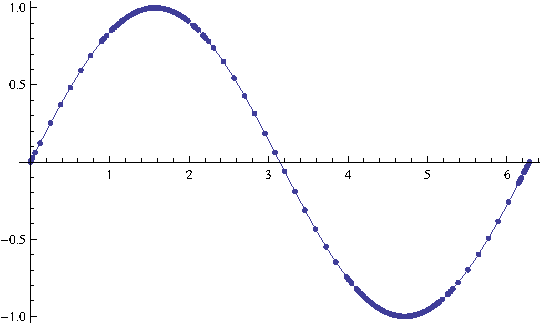
\includegraphics{figures/figmathematica_sinx}
\captionsetup{type=figure}%
			\caption{A graph of $y=\sin x$ generated by \textit{Mathematica}.}\label{fig:mathematica_sinx}
\end{minipage}
\vskip\baselineskip

How does \textit{Mathematica} know where the graph is ``curvy''? Calculus. When we study \textit{curvature} in a later chapter, we will see how the first and second derivatives of a function work together to provide a measurement of ``curviness.'' \textit{Mathematica} employs algorithms to determine regions of ``high curvature'' and plots extra points there.

Again, the goal of this section is not ``How to graph a function when there is no computer to help.'' Rather, the goal is ``Understand that the shape of the graph of a function is largely determined by understanding the behaviour of the function at a few key places.'' In Example \ref{ex_sketch3}, we were able to accurately sketch a complicated graph using only 5 points and knowledge of asymptotes!

There are many applications of our understanding of derivatives beyond curve sketching. The next chapter explores some of these applications, demonstrating just a few kinds of problems that can be solved with a basic knowledge of differentiation. 

\printexercises{exercises/03_05_exercises}
\ifthenelse{\boolean{1010}}{We have spent considerable time considering the derivatives of a function and their applications. In this section, we are going to starting thinking in ``the other direction.'' That is, given a function $f(x)$, we are going to consider functions $F(x)$ such that $F\primeskip'(x) = f(x)$. Here, we will only consider very basic examples, and leave most of the heavy lifting to later courses. The importance of antiderivatives becomes apparent in Math 1560, once integration and the Fundamental Theorem of Calculus have been introduced. More advanced techniques for finding antiderivatives are taught in Math 2560.}
{We have spent considerable time considering the derivatives of a function and their applications. In the following chapters, we are going to starting thinking in ``the other direction.'' That is, given a function $f(x)$, we are going to consider functions $F(x)$ such that $F\primeskip'(x) = f(x)$. There are numerous reasons this will prove to be useful: these functions will help us compute area, volume, mass, force, pressure, work, and much more.}



\section{Antiderivatives and Indefinite Integration}\label{sec:antider}

Given a function $y=f(x)$, a \textit{differential equation} is one that incorporates $y$, $x$, and the derivatives of $y$. For instance, a simple differential equation is: 
\[
y\primeskip' = 2x.
\]

Solving a differential equation amounts to finding a function $y$ that satisfies the given equation. Take a moment and consider that equation; can you find a function $y$ such that $y\primeskip' = 2x$?

Can you find another?

And yet another?

Hopefully one was able to come up with at least one solution: $y = x^2$. ``Finding another'' may have seemed impossible until one realizes that a function like $y=x^2+1$ also has a derivative of $2x$. Once that discovery is made, finding ``yet another'' is not difficult; the function $y = x^2 + 123,456,789$ also has a derivative of $2x$. The differential equation $y\primeskip' = 2x$ has many solutions. This leads us to some definitions.
%\enlargethispage{3\baselineskip}

\definition{def:antider}{Antiderivatives and Indefinite Integrals}
{Let a function $f(x)$ be given. An \textbf{antiderivative} of $f(x)$ is a function $F(x)$ such that $\Fp(x) = f(x)$.\index{antiderivative}\index{indefinite integral}\index{integration!indefinite}\\

The set of all antiderivatives of $f(x)$ is the \textbf{indefinite integral of $f$}, denoted by 
\[
\int f(x) \ dx.
\]
}

Make a note about our definition: we refer to \textit{an} antiderivative of $f$, as opposed to \textit{the} antiderivative of $f$, since there is \textit{always} an infinite number of them. We often use upper-case letters to denote antiderivatives.

Knowing one antiderivative of $f$ allows us to find infinitely more, simply by adding a constant. Not only does this give us \textit{more} antiderivatives, it gives us \textit{all} of them.

\theorem{thm:antideriv_const}{Antiderivative Forms}
{Let $F(x)$ and $G(x)$ be antiderivatives of $f(x)$ on an interval $I$. Then there exists a constant $C$ such that, on $I$,  
\[
G(x) = F(x) + C.
\]
}

Given a function $f$ defined on an interval $I$ and one of its antiderivatives $F$, we know \textit{all} antiderivatives of $f$ on $I$ have the form $F(x) + C$ for some constant $C$. Using Definition \ref{def:antider}, we can say that 
\[
\int f(x) \ dx = F(x) + C.
\]

Let's analyze this indefinite integral notation.\index{integration!notation}

\begin{center}
\myincludegraphics{figures/figanti1}
\captionsetup{type=figure}%
\caption{Understanding the indefinite integral notation.}\label{fig:anti1}
\end{center}

Figure \ref{fig:anti1} shows the typical notation of the indefinite integral. The integration symbol, $\int$, is in reality an ``elongated S,'' representing ``take the sum.'' We will later see how \textit{sums} and \textit{antiderivatives} are related.

The function we want to find an antiderivative of is called the \textit{integrand}. It contains the differential of the variable we are integrating with respect to. The $\int$ symbol and the differential $dx$ are not ``bookends'' with a function sandwiched in between; rather, the symbol $\int$ means ``find all antiderivatives of what follows,'' and the function $f(x)$ and $dx$ are multiplied together; the $dx$ does not ``just sit there.''

Let's practice using this notation.\\

\example{ex_anti2}{Evaluating indefinite integrals}{
Evaluate $\displaystyle \int \sin x\ dx.$}
{We are asked to find all functions $F(x)$ such that $\Fp(x) = \sin x$. Some thought will lead us to one solution: $F(x) = -\cos x$, because $\frac{d}{dx}(-\cos x) = \sin x$.

The indefinite integral of $\sin x$ is thus $-\cos x$, plus a constant of integration. So:
\[
\int \sin x \ dx = -\cos x + C.
\]
\vskip-\baselineskip
}\\

A commonly asked question is ``What happened to the $dx$?'' The unenlightened response is ``Don't worry about it. It just goes away.'' A full understanding includes the following.

This process of \textit{antidifferentiation} is really solving a \textit{differential} question. The integral 
\[
\int \sin x\ dx
\]
 presents us with a differential, $dy = \sin x\ dx$. It is asking: ``What is $y$?'' We found lots of solutions, all of the form $y = -\cos x+C$.

%We can view integration in the following way. 
Letting $dy = \sin x\ dx$,  rewrite 
\[
\int \sin x \ dx \quad \text{as}\quad \int  dy.
\]
This is asking: ``What functions have a differential of the form $dy$?'' The answer is ``Functions of the form $y+C$, where $C$ is a constant.'' What is $y$? We have lots of choices, all differing by a constant; the simplest choice is $y = -\cos x$.

Understanding all of this is more important later as we try to find antiderivatives of more complicated functions. In this section, we will simply explore the rules of indefinite integration, and one can succeed for now with answering ``What happened to the $dx$?'' with ``It went away.''

Let's practice once more before stating integration rules.\\

\example{ex_anti3}{Evaluating indefinite integrals}{
Evaluate $\ds \int (3x^2 + 4x+5)\ dx$.}
{We seek a function $F(x)$ whose derivative is $3x^2+4x+5$. When taking derivatives, we can consider functions term--by--term, so we can likely do that here.

What functions have a derivative of $3x^2$? Some thought will lead us to a cubic, specifically $x^3+C_1$, where $C_1$ is a constant. 

What functions have a derivative of $4x$? Here the $x$ term is raised to the first power, so we likely seek a quadratic. Some thought should lead us to $2x^2+C_2$, where $C_2$ is a constant.

Finally, what functions have a derivative of $5$? Functions of the form $5x+C_3$, where $C_3$ is a constant.

Our answer appears to be 
\[
\int (3x^2+4x+5)\ dx = x^3+C_1+2x^2+C_2+5x+C_3.
\]
 We do not need three separate constants of integration; combine them as one constant, giving the final answer of 
\[
\int (3x^2+4x+5)\ dx = x^3+2x^2+5x+C.
\]

It is easy to verify our answer; take the derivative of $x^3+2x^3+5x+C$ and see we indeed get $3x^2+4x+5$.
}\\

This final step of ``verifying our answer'' is important both practically and theoretically. In general, taking derivatives is easier than finding antiderivatives so checking our work is easy and vital as we learn.

We also see that taking the derivative of our answer returns the function in the integrand. Thus we can say that: 
\[
\frac{d}{dx}\left(\int f(x)\ dx\right) = f(x).
\]
Differentiation ``undoes'' the work done by antidifferentiation. 

\ifthenelse{\boolean{1010}}{For ease of reference, and to stress the relationship between derivatives and antiderivatives, we include below a list of many of the common differentiation rules we have learned, along with the corresponding antidifferentiation rules.}
{Theorem \ref{thm:deriv_glossary} gave a list of the derivatives of common functions we had learned at that point. We restate part of that list here to stress the relationship between derivatives and antiderivatives. This list will also be useful as a glossary of common antiderivatives as we learn.}

\newlength{\bh}%box height
\newlength{\bd}%box depth
\settoheight{\bh}{$\frac{d}{dx}$}
\settodepth{\bd}{$\frac{d}{dx}$}

%\newcommand{\myrule}{\rule[-\bd]{0pt}{\bh+\bd}}%\ $\frac{d}{dx}$
%\newcommand{\myrule}{\rule[-4pt]{0pt}{13pt}}%\ $\frac{d}{dx}$

\theorem{thm:indef_alg}{Derivatives and Antiderivatives}
{\begin{minipage}[t]{.45\specialboxlength}
Common Differentiation Rules\rule[-2pt]{0pt}{1pt}
\begin{enumerate}
\item \myrule$\frac{d}{dx}\big(cf(x) \big) = c\cdot \fp(x)$
\item \myrule$\frac{d}{dx}\big(f(x)\pm g(x) \big) = $
\vskip .05\baselineskip
\myrule$\fp(x)\pm g'(x)$
\item $\frac{d}{dx}\big(C \big) = 0$\myrule
\item $\frac{d}{dx}\big(x \big) = 1$\myrule
\item $\frac{d}{dx}\big(x^n \big) = n\cdot x^{n-1}$\myrule
\item $\frac{d}{dx}\big(\sin x \big) = \cos x$\myrule
\item $\frac{d}{dx}\big(\cos x \big) = -\sin x$\myrule
\item $\frac{d}{dx}\big(\tan x \big) = \sec^2 x$\myrule
\item $\frac{d}{dx}\big(\csc x \big) = -\csc x\cot x$\myrule
\item $\frac{d}{dx}\big(\sec x \big) = \sec x\tan x$\myrule
\item $\frac{d}{dx}\big(\cot x \big) = -\csc^2 x$\myrule
\item $\frac{d}{dx}\big(e^ x \big) = e^x$\myrule
\item $\frac{d}{dx}\big(a^x \big) = \ln a\cdot a^x$\myrule
\item $\frac{d}{dx}\big(\ln x \big) = \frac1 x$\myrule
\end{enumerate}
\end{minipage}
\begin{minipage}[t]{.55\specialboxlength}
Common Indefinite Integral Rules\rule[-2pt]{0pt}{1pt}
\begin{enumerate}
\item \myrule$\int c\cdot f(x)\ dx = c\cdot \int f(x)\ dx$
\item \myrule$\int \big(f(x)\pm g(x)\big)\ dx =$
\vskip .05\baselineskip
\myrule$ \int f(x)\ dx\pm \int g(x)\ dx$
\item $\int 0\ dx = C$\myrule
\item $\int 1\ dx = \int dx = x+C$\myrule
\item $\int x^n\ dx =\frac{1}{n+1}x^{n+1}+ C$\quad {\scriptsize ($n\neq -1$)}\myrule
\item $\int \cos x\ dx = \sin x+C$\myrule
\item $\int \sin x\ dx = -\cos x+C$\myrule
\item $\int \sec^2 x\ dx = \tan x+C$\myrule
\item $\int \csc x\cot  x\ dx = -\csc x+C$\myrule
\item $\int \sec x\tan x\ dx = \sec x+C$\myrule
\item $\int \csc^2 x\ dx = -\cot x+C$\myrule
\item $\int e^x\ dx = e^x+C$\myrule
\item $\int a^x\ dx = \frac{1}{\ln a}\cdot a^x+C$\myrule
\item $\int \frac{1}x\ dx = \ln |x|+C$\myrule
\end{enumerate}
\end{minipage}%\\
%
%\textit{\small (continued $\ldots$)}
}
%\addtocounter{theoremcounter}{-1}
%
%\theorem{thm:indef_algb}{Derivatives and Antiderivatives -- Continued}
%{\begin{minipage}[t]{.45\specialboxlength}
%Common Differentiation Rules\rule[-2pt]{0pt}{1pt}
%\begin{enumerate}\addtocounter{enumi}{5}
%%\item \myrule$\frac{d}{dx}\big(cf(x) \big) = c\cdot \fp(x)$
%%\item \myrule$\frac{d}{dx}\big(f(x)\pm g(x) \big) = $
%%\vskip .05\baselineskip
%%\myrule$\fp(x)\pm g'(x)$
%%\item $\frac{d}{dx}\big(C \big) = 0$\myrule
%%\item $\frac{d}{dx}\big(x \big) = 1$\myrule
%%\item $\frac{d}{dx}\big(x^n \big) = n\cdot x^{n-1}$\myrule
%\item $\frac{d}{dx}\big(\sin x \big) = \cos x$\myrule
%\item $\frac{d}{dx}\big(\cos x \big) = -\sin x$\myrule
%\item $\frac{d}{dx}\big(\tan x \big) = \sec^2 x$\myrule
%\item $\frac{d}{dx}\big(\csc x \big) = -\csc x\cot x$\myrule
%\item $\frac{d}{dx}\big(\sec x \big) = \sec x\tan x$\myrule
%\item $\frac{d}{dx}\big(\cot x \big) = -\csc^2 x$\myrule
%\item $\frac{d}{dx}\big(e^ x \big) = e^x$\myrule
%\item $\frac{d}{dx}\big(a^x \big) = \ln a\cdot a^x$\myrule
%\item $\frac{d}{dx}\big(\ln x \big) = \frac1 x$\myrule
%\end{enumerate}
%\end{minipage}
%\begin{minipage}[t]{.55\specialboxlength}
%Common Indefinite Integral Rules\rule[-2pt]{0pt}{1pt}
%\begin{enumerate}\addtocounter{enumi}{5}
%%\item \myrule$\int c\cdot f(x)\ dx = c\cdot \int f(x)\ dx$
%%\item \myrule$\int \big(f(x)\pm g(x)\big)\ dx =$
%%\vskip .05\baselineskip
%%\myrule$ \int f(x)\ dx\pm \int g(x)\ dx$
%%\item $\int 0\ dx = C$\myrule
%%\item $\int 1\ dx = \int dx = x+C$\myrule
%%\item $\int x^n\ dx =\frac{1}{n+1}x^{n+1}+ C$\quad {\scriptsize ($n\neq -1$)}\myrule
%\item $\int \cos x\ dx = \sin x+C$\myrule
%\item $\int \sin x\ dx = -\cos x+C$\myrule
%\item $\int \sec^2 x\ dx = \tan x+C$\myrule
%\item $\int \csc x\cot  x\ dx = -\csc x+C$\myrule
%\item $\int \sec x\tan x\ dx = \sec x+C$\myrule
%\item $\int \csc^2 x\ dx = -\cot x+C$\myrule
%\item $\int e^x\ dx = e^x+C$\myrule
%\item $\int a^x\ dx = \frac{1}{\ln a}\cdot a^x+C$\myrule
%\item $\int \frac{1}x\ dx = \ln |x|+C$\myrule
%\end{enumerate}
%\end{minipage}
%}

We highlight a few important points from Theorem \ref{thm:indef_alg}:
\begin{itemize}
	\item		Rule \#1 states $\int c\cdot f(x)\ dx = c\cdot \int f(x)\ dx$. This is the Constant Multiple Rule: \index{Constant Multiple Rule!of integration} we can temporarily ignore constants when finding antiderivatives, just as we did when computing derivatives (i.e., $\frac{d}{dx}\big(3x^2\big)$ is just as easy to compute as $\frac{d}{dx}\big(x^2\big)$). An example:
	\[
	\int 5\cos x\ dx = 5\cdot\int \cos x\ dx = 5\cdot (\sin x+C) = 5\sin x + C.
	\]
	In the last step we can consider the constant as also being multiplied by 5, but ``5 times a constant'' is still a constant, so we just write ``$C$\,''.
	\item		Rule \#2 is the Sum/Difference Rule:\index{integration!Sum/Difference Rule}\index{Sum/Difference Rule!of integration} we can split integrals apart when the integrand contains terms that are added/subtracted, as we did in Example \ref{ex_anti3}. So:
	\begin{align*}
	\int(3x^2+4x+5)\ dx &= \int 3x^2\ dx + \int 4x\ dx + \int 5\ dx \\
											&= 3\int x^2\ dx + 4\int x\ dx + \int 5 \ dx\\
											&= 3\cdot \frac13x^3 + 4\cdot \frac12x^2+5x+C\\
											&= x^3+2x^2+5x+C
	\end{align*}
	In practice we generally do not write out all these steps, but we demonstrate them here for completeness.
	\item		Rule \#5 is the Power Rule of indefinite integration.\index{integration!Power Rule}\index{Power Rule!integration} There are two important things to keep in mind:
		\begin{enumerate}
		\item		Notice the restriction that $n\neq -1$. This is important: $\int \frac{1}{x}\ dx \neq $ ``$\frac{1}{0}x^0+C$''; rather, see Rule \#14.
		\item		We are presenting antidifferentiation as the ``inverse operation'' of differentiation. Here is a useful quote to remember:
		\begin{quote}%\centering
		``Inverse operations do the opposite things in the opposite order.''
		\end{quote}
		When taking a derivative using the Power Rule, we \textbf{first} \textit{multiply} by the power, then \textbf{second} \textit{subtract} 1 from the power. To find the antiderivative, do the opposite things in the opposite order: \textbf{first} \textit{add} one to the power, then \textbf{second} \textit{divide} by the power.
			\end{enumerate}
		\item		Note that Rule \#14 incorporates the absolute value of $x$. The exercises will work the reader through why this is the case; for now, know the absolute value is important and cannot be ignored.
\end{itemize}

\enlargethispage{\baselineskip}
\vskip\baselineskip
\noindent\textbf{\large Initial Value Problems}
\vskip\baselineskip

In Section \ref{sec:basic_diff_rules} we saw that the derivative of a position function gave a velocity function, and the derivative of a velocity function describes  acceleration.\index{initial value problem} We can now go ``the other way:'' the antiderivative of an acceleration function gives a velocity function, etc. While there is just one derivative of a given function, there are infinitely many antiderivatives. Therefore we cannot ask ``What is \textit{the} velocity of an object whose acceleration is $-32$ft/s$^2$?'', since there is more than one answer. 

We can find \textit{the} answer if we provide more information with the question, as done in the following example. Often the additional information comes in the form of an \textit{initial value}, a value of the function that one knows beforehand.\\

\example{ex_anti4}{Solving initial value problems}{
The acceleration due to gravity of a falling object is $-32$ ft/s$^2$. At time $t=3$, a falling object had a velocity of $-10$ ft/s. Find the equation of the object's velocity.}
{We want to know a velocity function, $v(t)$. We know two things:
	\begin{itemize}
		\item		The acceleration, i.e., $v\primeskip'(t)= -32$, and
		\item		the velocity at a specific time, i.e., $v(3) = -10$.
	\end{itemize}
Using the first piece of information, we know that $v(t)$ is an antiderivative of $v\primeskip'(t)=-32$. So we begin by finding the indefinite integral of $-32$:
		\[
		\int (-32)\ dt = -32t+C=v(t).
		\]
Now we use the fact that $v(3)=-10$ to find $C$:
\begin{align*}
	v(t) &= -32t+C \\
	v(3) &= -10 \\
	-32(3)+C &= -10\\
	C &= 86
\end{align*}

Thus $v(t)= -32t+86$. We can use this equation to understand the motion of the object: when $t=0$, the object had a velocity of $v(0) = 86$ ft/s. Since the velocity is positive, the object was moving upward.

When did the object begin moving down? Immediately after $v(t) = 0$:
\[
-32t+86 = 0 \quad \Rightarrow\quad  t = \frac{43}{16}  \approx 2.69\text{s}.
\]
Recognize that we are able to determine quite a bit about the path of the object knowing just its acceleration and its velocity at a single point in time.
}\\

\example{ex_anti5}{Solving initial value problems}{
Find $f(t)$, given that $\fpp(t) = \cos t$, $\fp(0) = 3$ and $f(0) = 5$.}
{We start by finding $\fp(t)$, which is an antiderivative of $\fpp(t)$:
		\[
		\int \fpp(t)\ dt = \int \cos t\ dt = \sin t + C = \fp(t).
		\]
		
		So $\fp(t) = \sin t+C$ for the correct value of $C$. We are given that $\fp(0) = 3$, so:
		\[
		\fp(0) = 3 \quad \Rightarrow \quad \sin 0+C = 3 \quad \Rightarrow \quad C=3.
		\]
		Using the initial value, we have found $\fp(t) = \sin t+ 3.$
		
We now find $f(t)$ by integrating again.

%\enlargethispage{3\baselineskip}
\[
f(t)=\int \fp(t) \ dt = \int (\sin t+3)\ dt = -\cos t + 3t + C.
\] 
We are given that $f(0) = 5$, so
\begin{align*}
-\cos 0 + 3(0) + C &= 5 \\
-1 + C &= 5\\
C &= 6
\end{align*}
 Thus $f(t) = -\cos t + 3t + 6$.
}\\

This section introduced antiderivatives and the indefinite integral. We found they are needed when finding a function given information about its derivative(s). For instance, we found a velocity function given an acceleration function.

\ifthenelse{\boolean{1010}}{If you continue on to Math 1560, you will see how position and velocity are unexpectedly related by the areas of certain regions on a graph of the velocity function, and how the Fundamental Theorem of Calculus ties together areas and antiderivatives.}
{In the next section, we will see how position and velocity are unexpectedly related by the areas of certain regions on a graph of the velocity function. Then, in Section \ref{sec:FTC}, we will see how areas and antiderivatives are closely tied together. This connection is incredibly important, as indicated by the name of the theorem that describes it: The Fundamental Theorem of Calculus.}

\printexercises{exercises/05_01_exercises}

%%
%%%%\addtocounter{chapter}{3}

%
%\clearpage{\pagestyle{empty}\cleardoublepage}
%\chapter{Integration}\label{chapter:integration}
%\thispagestyle{empty}
%\addtocontents{toc}{\protect\thispagestyle{empty}}

%\ifthenelse{\boolean{1010}}{We have spent considerable time considering the derivatives of a function and their applications. In this section, we are going to starting thinking in ``the other direction.'' That is, given a function $f(x)$, we are going to consider functions $F(x)$ such that $F\primeskip'(x) = f(x)$. Here, we will only consider very basic examples, and leave most of the heavy lifting to later courses. The importance of antiderivatives becomes apparent in Math 1560, once integration and the Fundamental Theorem of Calculus have been introduced. More advanced techniques for finding antiderivatives are taught in Math 2560.}
{We have spent considerable time considering the derivatives of a function and their applications. In the following chapters, we are going to starting thinking in ``the other direction.'' That is, given a function $f(x)$, we are going to consider functions $F(x)$ such that $F\primeskip'(x) = f(x)$. There are numerous reasons this will prove to be useful: these functions will help us compute area, volume, mass, force, pressure, work, and much more.}



\section{Antiderivatives and Indefinite Integration}\label{sec:antider}

Given a function $y=f(x)$, a \textit{differential equation} is one that incorporates $y$, $x$, and the derivatives of $y$. For instance, a simple differential equation is: 
\[
y\primeskip' = 2x.
\]

Solving a differential equation amounts to finding a function $y$ that satisfies the given equation. Take a moment and consider that equation; can you find a function $y$ such that $y\primeskip' = 2x$?

Can you find another?

And yet another?

Hopefully one was able to come up with at least one solution: $y = x^2$. ``Finding another'' may have seemed impossible until one realizes that a function like $y=x^2+1$ also has a derivative of $2x$. Once that discovery is made, finding ``yet another'' is not difficult; the function $y = x^2 + 123,456,789$ also has a derivative of $2x$. The differential equation $y\primeskip' = 2x$ has many solutions. This leads us to some definitions.
%\enlargethispage{3\baselineskip}

\definition{def:antider}{Antiderivatives and Indefinite Integrals}
{Let a function $f(x)$ be given. An \textbf{antiderivative} of $f(x)$ is a function $F(x)$ such that $\Fp(x) = f(x)$.\index{antiderivative}\index{indefinite integral}\index{integration!indefinite}\\

The set of all antiderivatives of $f(x)$ is the \textbf{indefinite integral of $f$}, denoted by 
\[
\int f(x) \ dx.
\]
}

Make a note about our definition: we refer to \textit{an} antiderivative of $f$, as opposed to \textit{the} antiderivative of $f$, since there is \textit{always} an infinite number of them. We often use upper-case letters to denote antiderivatives.

Knowing one antiderivative of $f$ allows us to find infinitely more, simply by adding a constant. Not only does this give us \textit{more} antiderivatives, it gives us \textit{all} of them.

\theorem{thm:antideriv_const}{Antiderivative Forms}
{Let $F(x)$ and $G(x)$ be antiderivatives of $f(x)$ on an interval $I$. Then there exists a constant $C$ such that, on $I$,  
\[
G(x) = F(x) + C.
\]
}

Given a function $f$ defined on an interval $I$ and one of its antiderivatives $F$, we know \textit{all} antiderivatives of $f$ on $I$ have the form $F(x) + C$ for some constant $C$. Using Definition \ref{def:antider}, we can say that 
\[
\int f(x) \ dx = F(x) + C.
\]

Let's analyze this indefinite integral notation.\index{integration!notation}

\begin{center}
\myincludegraphics{figures/figanti1}
\captionsetup{type=figure}%
\caption{Understanding the indefinite integral notation.}\label{fig:anti1}
\end{center}

Figure \ref{fig:anti1} shows the typical notation of the indefinite integral. The integration symbol, $\int$, is in reality an ``elongated S,'' representing ``take the sum.'' We will later see how \textit{sums} and \textit{antiderivatives} are related.

The function we want to find an antiderivative of is called the \textit{integrand}. It contains the differential of the variable we are integrating with respect to. The $\int$ symbol and the differential $dx$ are not ``bookends'' with a function sandwiched in between; rather, the symbol $\int$ means ``find all antiderivatives of what follows,'' and the function $f(x)$ and $dx$ are multiplied together; the $dx$ does not ``just sit there.''

Let's practice using this notation.\\

\example{ex_anti2}{Evaluating indefinite integrals}{
Evaluate $\displaystyle \int \sin x\ dx.$}
{We are asked to find all functions $F(x)$ such that $\Fp(x) = \sin x$. Some thought will lead us to one solution: $F(x) = -\cos x$, because $\frac{d}{dx}(-\cos x) = \sin x$.

The indefinite integral of $\sin x$ is thus $-\cos x$, plus a constant of integration. So:
\[
\int \sin x \ dx = -\cos x + C.
\]
\vskip-\baselineskip
}\\

A commonly asked question is ``What happened to the $dx$?'' The unenlightened response is ``Don't worry about it. It just goes away.'' A full understanding includes the following.

This process of \textit{antidifferentiation} is really solving a \textit{differential} question. The integral 
\[
\int \sin x\ dx
\]
 presents us with a differential, $dy = \sin x\ dx$. It is asking: ``What is $y$?'' We found lots of solutions, all of the form $y = -\cos x+C$.

%We can view integration in the following way. 
Letting $dy = \sin x\ dx$,  rewrite 
\[
\int \sin x \ dx \quad \text{as}\quad \int  dy.
\]
This is asking: ``What functions have a differential of the form $dy$?'' The answer is ``Functions of the form $y+C$, where $C$ is a constant.'' What is $y$? We have lots of choices, all differing by a constant; the simplest choice is $y = -\cos x$.

Understanding all of this is more important later as we try to find antiderivatives of more complicated functions. In this section, we will simply explore the rules of indefinite integration, and one can succeed for now with answering ``What happened to the $dx$?'' with ``It went away.''

Let's practice once more before stating integration rules.\\

\example{ex_anti3}{Evaluating indefinite integrals}{
Evaluate $\ds \int (3x^2 + 4x+5)\ dx$.}
{We seek a function $F(x)$ whose derivative is $3x^2+4x+5$. When taking derivatives, we can consider functions term--by--term, so we can likely do that here.

What functions have a derivative of $3x^2$? Some thought will lead us to a cubic, specifically $x^3+C_1$, where $C_1$ is a constant. 

What functions have a derivative of $4x$? Here the $x$ term is raised to the first power, so we likely seek a quadratic. Some thought should lead us to $2x^2+C_2$, where $C_2$ is a constant.

Finally, what functions have a derivative of $5$? Functions of the form $5x+C_3$, where $C_3$ is a constant.

Our answer appears to be 
\[
\int (3x^2+4x+5)\ dx = x^3+C_1+2x^2+C_2+5x+C_3.
\]
 We do not need three separate constants of integration; combine them as one constant, giving the final answer of 
\[
\int (3x^2+4x+5)\ dx = x^3+2x^2+5x+C.
\]

It is easy to verify our answer; take the derivative of $x^3+2x^3+5x+C$ and see we indeed get $3x^2+4x+5$.
}\\

This final step of ``verifying our answer'' is important both practically and theoretically. In general, taking derivatives is easier than finding antiderivatives so checking our work is easy and vital as we learn.

We also see that taking the derivative of our answer returns the function in the integrand. Thus we can say that: 
\[
\frac{d}{dx}\left(\int f(x)\ dx\right) = f(x).
\]
Differentiation ``undoes'' the work done by antidifferentiation. 

\ifthenelse{\boolean{1010}}{For ease of reference, and to stress the relationship between derivatives and antiderivatives, we include below a list of many of the common differentiation rules we have learned, along with the corresponding antidifferentiation rules.}
{Theorem \ref{thm:deriv_glossary} gave a list of the derivatives of common functions we had learned at that point. We restate part of that list here to stress the relationship between derivatives and antiderivatives. This list will also be useful as a glossary of common antiderivatives as we learn.}

\newlength{\bh}%box height
\newlength{\bd}%box depth
\settoheight{\bh}{$\frac{d}{dx}$}
\settodepth{\bd}{$\frac{d}{dx}$}

%\newcommand{\myrule}{\rule[-\bd]{0pt}{\bh+\bd}}%\ $\frac{d}{dx}$
%\newcommand{\myrule}{\rule[-4pt]{0pt}{13pt}}%\ $\frac{d}{dx}$

\theorem{thm:indef_alg}{Derivatives and Antiderivatives}
{\begin{minipage}[t]{.45\specialboxlength}
Common Differentiation Rules\rule[-2pt]{0pt}{1pt}
\begin{enumerate}
\item \myrule$\frac{d}{dx}\big(cf(x) \big) = c\cdot \fp(x)$
\item \myrule$\frac{d}{dx}\big(f(x)\pm g(x) \big) = $
\vskip .05\baselineskip
\myrule$\fp(x)\pm g'(x)$
\item $\frac{d}{dx}\big(C \big) = 0$\myrule
\item $\frac{d}{dx}\big(x \big) = 1$\myrule
\item $\frac{d}{dx}\big(x^n \big) = n\cdot x^{n-1}$\myrule
\item $\frac{d}{dx}\big(\sin x \big) = \cos x$\myrule
\item $\frac{d}{dx}\big(\cos x \big) = -\sin x$\myrule
\item $\frac{d}{dx}\big(\tan x \big) = \sec^2 x$\myrule
\item $\frac{d}{dx}\big(\csc x \big) = -\csc x\cot x$\myrule
\item $\frac{d}{dx}\big(\sec x \big) = \sec x\tan x$\myrule
\item $\frac{d}{dx}\big(\cot x \big) = -\csc^2 x$\myrule
\item $\frac{d}{dx}\big(e^ x \big) = e^x$\myrule
\item $\frac{d}{dx}\big(a^x \big) = \ln a\cdot a^x$\myrule
\item $\frac{d}{dx}\big(\ln x \big) = \frac1 x$\myrule
\end{enumerate}
\end{minipage}
\begin{minipage}[t]{.55\specialboxlength}
Common Indefinite Integral Rules\rule[-2pt]{0pt}{1pt}
\begin{enumerate}
\item \myrule$\int c\cdot f(x)\ dx = c\cdot \int f(x)\ dx$
\item \myrule$\int \big(f(x)\pm g(x)\big)\ dx =$
\vskip .05\baselineskip
\myrule$ \int f(x)\ dx\pm \int g(x)\ dx$
\item $\int 0\ dx = C$\myrule
\item $\int 1\ dx = \int dx = x+C$\myrule
\item $\int x^n\ dx =\frac{1}{n+1}x^{n+1}+ C$\quad {\scriptsize ($n\neq -1$)}\myrule
\item $\int \cos x\ dx = \sin x+C$\myrule
\item $\int \sin x\ dx = -\cos x+C$\myrule
\item $\int \sec^2 x\ dx = \tan x+C$\myrule
\item $\int \csc x\cot  x\ dx = -\csc x+C$\myrule
\item $\int \sec x\tan x\ dx = \sec x+C$\myrule
\item $\int \csc^2 x\ dx = -\cot x+C$\myrule
\item $\int e^x\ dx = e^x+C$\myrule
\item $\int a^x\ dx = \frac{1}{\ln a}\cdot a^x+C$\myrule
\item $\int \frac{1}x\ dx = \ln |x|+C$\myrule
\end{enumerate}
\end{minipage}%\\
%
%\textit{\small (continued $\ldots$)}
}
%\addtocounter{theoremcounter}{-1}
%
%\theorem{thm:indef_algb}{Derivatives and Antiderivatives -- Continued}
%{\begin{minipage}[t]{.45\specialboxlength}
%Common Differentiation Rules\rule[-2pt]{0pt}{1pt}
%\begin{enumerate}\addtocounter{enumi}{5}
%%\item \myrule$\frac{d}{dx}\big(cf(x) \big) = c\cdot \fp(x)$
%%\item \myrule$\frac{d}{dx}\big(f(x)\pm g(x) \big) = $
%%\vskip .05\baselineskip
%%\myrule$\fp(x)\pm g'(x)$
%%\item $\frac{d}{dx}\big(C \big) = 0$\myrule
%%\item $\frac{d}{dx}\big(x \big) = 1$\myrule
%%\item $\frac{d}{dx}\big(x^n \big) = n\cdot x^{n-1}$\myrule
%\item $\frac{d}{dx}\big(\sin x \big) = \cos x$\myrule
%\item $\frac{d}{dx}\big(\cos x \big) = -\sin x$\myrule
%\item $\frac{d}{dx}\big(\tan x \big) = \sec^2 x$\myrule
%\item $\frac{d}{dx}\big(\csc x \big) = -\csc x\cot x$\myrule
%\item $\frac{d}{dx}\big(\sec x \big) = \sec x\tan x$\myrule
%\item $\frac{d}{dx}\big(\cot x \big) = -\csc^2 x$\myrule
%\item $\frac{d}{dx}\big(e^ x \big) = e^x$\myrule
%\item $\frac{d}{dx}\big(a^x \big) = \ln a\cdot a^x$\myrule
%\item $\frac{d}{dx}\big(\ln x \big) = \frac1 x$\myrule
%\end{enumerate}
%\end{minipage}
%\begin{minipage}[t]{.55\specialboxlength}
%Common Indefinite Integral Rules\rule[-2pt]{0pt}{1pt}
%\begin{enumerate}\addtocounter{enumi}{5}
%%\item \myrule$\int c\cdot f(x)\ dx = c\cdot \int f(x)\ dx$
%%\item \myrule$\int \big(f(x)\pm g(x)\big)\ dx =$
%%\vskip .05\baselineskip
%%\myrule$ \int f(x)\ dx\pm \int g(x)\ dx$
%%\item $\int 0\ dx = C$\myrule
%%\item $\int 1\ dx = \int dx = x+C$\myrule
%%\item $\int x^n\ dx =\frac{1}{n+1}x^{n+1}+ C$\quad {\scriptsize ($n\neq -1$)}\myrule
%\item $\int \cos x\ dx = \sin x+C$\myrule
%\item $\int \sin x\ dx = -\cos x+C$\myrule
%\item $\int \sec^2 x\ dx = \tan x+C$\myrule
%\item $\int \csc x\cot  x\ dx = -\csc x+C$\myrule
%\item $\int \sec x\tan x\ dx = \sec x+C$\myrule
%\item $\int \csc^2 x\ dx = -\cot x+C$\myrule
%\item $\int e^x\ dx = e^x+C$\myrule
%\item $\int a^x\ dx = \frac{1}{\ln a}\cdot a^x+C$\myrule
%\item $\int \frac{1}x\ dx = \ln |x|+C$\myrule
%\end{enumerate}
%\end{minipage}
%}

We highlight a few important points from Theorem \ref{thm:indef_alg}:
\begin{itemize}
	\item		Rule \#1 states $\int c\cdot f(x)\ dx = c\cdot \int f(x)\ dx$. This is the Constant Multiple Rule: \index{Constant Multiple Rule!of integration} we can temporarily ignore constants when finding antiderivatives, just as we did when computing derivatives (i.e., $\frac{d}{dx}\big(3x^2\big)$ is just as easy to compute as $\frac{d}{dx}\big(x^2\big)$). An example:
	\[
	\int 5\cos x\ dx = 5\cdot\int \cos x\ dx = 5\cdot (\sin x+C) = 5\sin x + C.
	\]
	In the last step we can consider the constant as also being multiplied by 5, but ``5 times a constant'' is still a constant, so we just write ``$C$\,''.
	\item		Rule \#2 is the Sum/Difference Rule:\index{integration!Sum/Difference Rule}\index{Sum/Difference Rule!of integration} we can split integrals apart when the integrand contains terms that are added/subtracted, as we did in Example \ref{ex_anti3}. So:
	\begin{align*}
	\int(3x^2+4x+5)\ dx &= \int 3x^2\ dx + \int 4x\ dx + \int 5\ dx \\
											&= 3\int x^2\ dx + 4\int x\ dx + \int 5 \ dx\\
											&= 3\cdot \frac13x^3 + 4\cdot \frac12x^2+5x+C\\
											&= x^3+2x^2+5x+C
	\end{align*}
	In practice we generally do not write out all these steps, but we demonstrate them here for completeness.
	\item		Rule \#5 is the Power Rule of indefinite integration.\index{integration!Power Rule}\index{Power Rule!integration} There are two important things to keep in mind:
		\begin{enumerate}
		\item		Notice the restriction that $n\neq -1$. This is important: $\int \frac{1}{x}\ dx \neq $ ``$\frac{1}{0}x^0+C$''; rather, see Rule \#14.
		\item		We are presenting antidifferentiation as the ``inverse operation'' of differentiation. Here is a useful quote to remember:
		\begin{quote}%\centering
		``Inverse operations do the opposite things in the opposite order.''
		\end{quote}
		When taking a derivative using the Power Rule, we \textbf{first} \textit{multiply} by the power, then \textbf{second} \textit{subtract} 1 from the power. To find the antiderivative, do the opposite things in the opposite order: \textbf{first} \textit{add} one to the power, then \textbf{second} \textit{divide} by the power.
			\end{enumerate}
		\item		Note that Rule \#14 incorporates the absolute value of $x$. The exercises will work the reader through why this is the case; for now, know the absolute value is important and cannot be ignored.
\end{itemize}

\enlargethispage{\baselineskip}
\vskip\baselineskip
\noindent\textbf{\large Initial Value Problems}
\vskip\baselineskip

In Section \ref{sec:basic_diff_rules} we saw that the derivative of a position function gave a velocity function, and the derivative of a velocity function describes  acceleration.\index{initial value problem} We can now go ``the other way:'' the antiderivative of an acceleration function gives a velocity function, etc. While there is just one derivative of a given function, there are infinitely many antiderivatives. Therefore we cannot ask ``What is \textit{the} velocity of an object whose acceleration is $-32$ft/s$^2$?'', since there is more than one answer. 

We can find \textit{the} answer if we provide more information with the question, as done in the following example. Often the additional information comes in the form of an \textit{initial value}, a value of the function that one knows beforehand.\\

\example{ex_anti4}{Solving initial value problems}{
The acceleration due to gravity of a falling object is $-32$ ft/s$^2$. At time $t=3$, a falling object had a velocity of $-10$ ft/s. Find the equation of the object's velocity.}
{We want to know a velocity function, $v(t)$. We know two things:
	\begin{itemize}
		\item		The acceleration, i.e., $v\primeskip'(t)= -32$, and
		\item		the velocity at a specific time, i.e., $v(3) = -10$.
	\end{itemize}
Using the first piece of information, we know that $v(t)$ is an antiderivative of $v\primeskip'(t)=-32$. So we begin by finding the indefinite integral of $-32$:
		\[
		\int (-32)\ dt = -32t+C=v(t).
		\]
Now we use the fact that $v(3)=-10$ to find $C$:
\begin{align*}
	v(t) &= -32t+C \\
	v(3) &= -10 \\
	-32(3)+C &= -10\\
	C &= 86
\end{align*}

Thus $v(t)= -32t+86$. We can use this equation to understand the motion of the object: when $t=0$, the object had a velocity of $v(0) = 86$ ft/s. Since the velocity is positive, the object was moving upward.

When did the object begin moving down? Immediately after $v(t) = 0$:
\[
-32t+86 = 0 \quad \Rightarrow\quad  t = \frac{43}{16}  \approx 2.69\text{s}.
\]
Recognize that we are able to determine quite a bit about the path of the object knowing just its acceleration and its velocity at a single point in time.
}\\

\example{ex_anti5}{Solving initial value problems}{
Find $f(t)$, given that $\fpp(t) = \cos t$, $\fp(0) = 3$ and $f(0) = 5$.}
{We start by finding $\fp(t)$, which is an antiderivative of $\fpp(t)$:
		\[
		\int \fpp(t)\ dt = \int \cos t\ dt = \sin t + C = \fp(t).
		\]
		
		So $\fp(t) = \sin t+C$ for the correct value of $C$. We are given that $\fp(0) = 3$, so:
		\[
		\fp(0) = 3 \quad \Rightarrow \quad \sin 0+C = 3 \quad \Rightarrow \quad C=3.
		\]
		Using the initial value, we have found $\fp(t) = \sin t+ 3.$
		
We now find $f(t)$ by integrating again.

%\enlargethispage{3\baselineskip}
\[
f(t)=\int \fp(t) \ dt = \int (\sin t+3)\ dt = -\cos t + 3t + C.
\] 
We are given that $f(0) = 5$, so
\begin{align*}
-\cos 0 + 3(0) + C &= 5 \\
-1 + C &= 5\\
C &= 6
\end{align*}
 Thus $f(t) = -\cos t + 3t + 6$.
}\\

This section introduced antiderivatives and the indefinite integral. We found they are needed when finding a function given information about its derivative(s). For instance, we found a velocity function given an acceleration function.

\ifthenelse{\boolean{1010}}{If you continue on to Math 1560, you will see how position and velocity are unexpectedly related by the areas of certain regions on a graph of the velocity function, and how the Fundamental Theorem of Calculus ties together areas and antiderivatives.}
{In the next section, we will see how position and velocity are unexpectedly related by the areas of certain regions on a graph of the velocity function. Then, in Section \ref{sec:FTC}, we will see how areas and antiderivatives are closely tied together. This connection is incredibly important, as indicated by the name of the theorem that describes it: The Fundamental Theorem of Calculus.}

\printexercises{exercises/05_01_exercises}

%\addtocontents{toc}{\protect\thispagestyle{empty}}
%\section{The Definite Integral}\label{sec:def_int}

We start with an easy problem. An object travels in a straight line at a constant velocity of 5 ft/s for 10 seconds. How far away from its starting point is the object?

We approach this problem with the familiar ``Distance $=$ Rate $\times$ Time'' equation. In this case, Distance = 5ft/s $\times$ 10s $=$ 50 feet.

It is interesting to note that this solution of 50 feet can be represented graphically. Consider Figure \ref{fig:defint1}, where the constant velocity of 5ft/s is graphed on the axes. Shading the area under the line from $t=0$ to $t=10$ gives a rectangle with an area of 50 square units; when one considers the units of the axes, we can say this area represents 50 ft.

\mfigure{.8}{The area under a constant velocity function corresponds to distance travelled.}{fig:defint1}{figures/figdefint1}

Now consider a slightly harder situation (and not particularly realistic): an object travels in a straight line with a constant velocity of 5ft/s for 10 seconds, then instantly reverses course at a rate of 2ft/s for 4 seconds. (Since the object is travelling in the opposite direction when reversing course, we say the velocity is a constant $-2$ft/s.) How far away from the starting point is the object -- what is its \textit{displacement}?

Here we use ``Distance $=$ Rate$_1$ $\times$ Time$_1$ + Rate$_2$ $\times$ Time$_2$,'' which is 
	\[
	\text{Distance } \ = 5\cdot10 + (-2)\cdot 4 = 42\text{ ft.}
	\] 
Hence the object is 42 feet from its starting location.

We can again depict this situation graphically. In Figure \ref{fig:defint2} we have the velocities graphed as straight lines on $[0,10]$ and $[10,14]$, respectively. The displacement of the object is 
		\begin{center}``Area above the $t$--axis \quad $-$\quad Area below the $t$--axis,''
		\end{center}
which is easy to calculate as $50-8=42$ feet.

\mfigure{.55}{The total displacement is the area above the $t$--axis minus the area below the $t$--axis.}{fig:defint2}{figures/figdefint2}

Now consider a more difficult problem.\\

\example{ex_defint3}{Finding position using velocity}{
The velocity of an object moving straight up/down under the acceleration of gravity is given as $v(t) = -32t+48$, where time $t$ is given in seconds and velocity is in ft/s. When $t=0$, the object had a height of 0 ft.
		\begin{enumerate}
		\item		What was the initial velocity of the object?
		\item		What was the maximum height of the object?
		\item		What was the height of the object at time $t=2$?
		\end{enumerate}
		
}
{It is straightforward to find the initial velocity; at time $t=0$, $v(0) =-32\cdot 0+48 = 48 $ ft/s.

To answer questions about the height of the object, we need to find the object's position function $s(t)$. This is an initial value problem, which we studied in the previous section. We are told the initial height is 0, i.e., $s(0) = 0$. We know $s\primeskip'(t) = v(t) = -32t+48$. To find $s$, we find the indefinite integral of $v(t)$:
		\[
		\int v(t)\ dt = \int (-32t+48)\ dt = -16t^2+48t+C = s(t).
		\]
Since $s(0) = 0$, we conclude that $C=0$ and $s(t) = -16t^2+48t$.

To find the maximum height of the object, we need to find the maximum of $s$. Recalling our work finding extreme values, we find the critical points of $s$ by setting its derivative equal to 0 and solving for $t$:
		\[
		s\primeskip'(t) = -32t+48 = 0 \quad \Rightarrow \quad t=48/32 = 1.5\text{s}.
		\]
(Notice how we ended up just finding when the velocity was 0ft/s!) The first derivative test shows this is a maximum, so the maximum height of the object is found at 
\[
s(1.5) = -16(1.5)^2+48(1.5)=36\text{ft}.
\]
The height at time $t=2$ is now straightforward to compute: it is $s(2) = 32$ft.\\

While we have answered all three questions, let's look at them again graphically, using the concepts of area that we explored earlier.


Figure \ref{fig:defint3} shows a graph of $v(t)$ on axes from $t=0$ to $t=3$. It is again straightforward to find $v(0)$. How can we use the graph to find the maximum height of the object?

\mfigure{.5}{A graph of $v(t)=-32t+48$; the shaded areas help determine displacement.}{fig:defint3}{figures/figdefint3}

Recall how in our previous work that the displacement of the object (in this case, its height) was found as the area under the velocity curve, as shaded in the figure. Moreover, the area between the curve and the $t$--axis that is below the $t$--axis counted as ``negative'' area. That is, it represents the object coming back toward its starting position. So to find the maximum distance from the starting point -- the maximum height -- we find the area under the velocity line that is above the $t$--axis, i.e., from $t=0$ to $t=1.5$. This region is a triangle; its area is 
\[
\text{Area } = \frac12\text{Base} \times \text{Height} =\frac12\times 1.5\text{s}\times 48\text{ft/s} = 36\text{ft},
\]
which matches our previous calculation of the maximum height.

%\enlargethispage{3\baselineskip}
%\drawexampleline
%Finally, we find the total \textit{signed} area under the velocity function from $t=0$ to $t=2$ to find the $s(2)$, the height at $t=2$, which is a displacement, the distance from the current position to the starting position. 
Finally, to find the height of the object at time $t=2$ we calculate the total ``signed area'' (where some area is negative) under the velocity function from $t=0$ to $t=2$. This signed area is equal to $s(2)$, the displacement (i.e., signed distance) from the starting position at $t=0$ to the position at time $t=2$. That is,
	\begin{center}
	Displacement = Area above the $t$--axis $-$ Area below $t$--axis.
	\end{center}
	The regions are triangles, and we find 
	\[
	\text{Displacement} = \frac12(1.5\text{s})(48\text{ft/s}) - \frac12(.5\text{s})(16\text{ft/s}) = 32\text{ft}.
	\]
This also matches our previous calculation of the height at $t=2$.

Notice how we answered each question in this example in two ways. Our first method was to manipulate equations using our understanding of antiderivatives and derivatives. Our second method was geometric: we answered questions looking at a graph and finding the areas of certain regions of this graph.
%\vskip-\baselineskip
}\\

The above example does not \textit{prove} a relationship between area under a velocity function and displacement, but it does imply a relationship exists. Section \ref{sec:FTC} will fully establish fact that the area under a velocity function is displacement.

Given a graph of a function $y=f(x)$, we will find that there is great use in computing the area between the curve $y=f(x)$ and the $x$-axis. Because of this, we need to define some terms.

\definition{def:def_int}{The Definite Integral, Total Signed Area}
{Let $y=f(x)$ be defined on a closed interval $[a,b]$. The \textbf{total signed area from $x=a$ to $x=b$ under $f$} is:\index{integration!definite}\index{definite integral}\index{signed area}\index{total signed area}\index{integration!notation}\index{integration!area}

\noindent\parbox{\specialboxlength}{\centering (area  under $f$ and above the $x$--axis on $[a,b]$) $-$ (area above $f$ and under the $x$--axis on $[a,b]$).}\\

The \textbf{definite integral of $f$ on $[a,b]$} is the total signed area of $f$ on $[a,b]$, denoted 
\[
\int_a^b f(x)\ dx,
\]
where $a$ and $b$ are the \textbf{bounds of integration.}
}

By our definition, the definite integral gives the ``signed area under $f$.'' We usually drop the word ``signed'' when talking about the definite integral, and simply say the definite integral gives ``the area under $f$\,'' or, more commonly, ``the area under the curve.''

The previous section introduced the indefinite integral, which related to antiderivatives. We have now defined the definite integral, which relates to areas under a function. The two are very much related, as we'll see when we learn the Fundamental Theorem of Calculus in Section \ref{sec:FTC}. Recall that earlier we said that the ``$\int$'' symbol was an ``elongated S'' that represented finding a ``sum.'' In the context of the definite integral, this notation makes a bit more sense, as we are adding up areas under the function $f$.

We practice using this notation.\\

\example{ex_defint4}{Evaluating definite integrals}{
Consider the function $f$ given in Figure \ref{fig:defint4}.

\mfigure{.4}{A graph of $f(x)$ in Example \ref{ex_defint4}.}{fig:defint4}{figures/figdefint4}
 Find:

\noindent\begin{minipage}[t]{.45\textwidth}
\begin{enumerate}
		\item		$\ds \int_0^3 f(x)\ dx$
		\item		$\ds \int_3^5 f(x)\ dx$
		\item		$\ds \int_0^5 f(x)\ dx$
\end{enumerate}
\end{minipage}\hskip .05\textwidth
\begin{minipage}[t]{.45\textwidth}
		\begin{enumerate}\addtocounter{enumi}{3}
		\item		$\ds \int_0^3 5f(x)\ dx$
		\item		$\ds \int_1^1 f(x) \ dx$
\end{enumerate}
\end{minipage}

}
{\begin{enumerate}
		\item		$ \int_0^3 f(x)\ dx$ is the area under $f$ on the interval $[0,3]$. This region is a triangle, so the area is $\int_0^3 f(x)\ dx=\frac12(3)(1) = 1.5$. 
		\item		$\int_3^5 f(x)\ dx$ represents the area of the triangle found under the $x$--axis on $[3,5]$. The area is $\frac12(2)(1) = 1$; since it is found \textit{under} the $x$--axis, this is ``negative area.'' Therefore $ \int_3^5 f(x)\ dx = -1$.
		\item		$ \int_0^5f(x)\ dx$ is the total signed area under $f$ on $[0,5]$. This is $1.5 + (-1) = 0.5$.
		\item		$ \int_0^35f(x)\ dx$ is the area under $5f$ on $[0,3]$. This is sketched in Figure \ref{fig:defint4a}. Again, the region is a triangle, with height 5 times that of the height of the original triangle. Thus the area is $ \int_0^35f(x)\ dx = \frac12(15)(1) = 7.5.$
		
\mfigure{.2}{A graph of $5f$ in Example \ref{ex_defint4}. (Yes, it looks just like the graph of $f$ in Figure \ref{fig:defint4}, just with a different $y$-scale.)}{fig:defint4a}{figures/figdefint4a}		
		
		\item		$\int_1^1f(x)\ dx$ is the area under $f$ on the ``interval'' $[1,1]$. This describes a line segment, not a region; it has no width. Therefore the area is 0.
\end{enumerate}
\vskip-\baselineskip
}\\

This example illustrates some of the properties of the definite integral, given here.

\theorem{thm:defintprop}{Properties of the Definite Integral}
{Let $f$ and $g$ be defined on a closed interval $I$ that contains the values $a$, $b$ and $c$, and let $k$ be a constant. The following hold:\index{integration!definite!properties}\index{definite integral!properties}
		\begin{enumerate}
		\item		$\ds \int_a^a f(x)\ dx = 0$
		\item		$\ds \int_a^b f(x)\ dx + \int_b^c f(x)\ dx = \int_a^cf(x)\ dx$
		\item		$\ds \int_a^bf(x)\ dx = -\int_b^a f(x)\ dx$
		\item		$\ds \int_a^b\big(f(x)\pm g(x)\big)\ dx = \int_a^bf(x)\ dx \pm \int_a^bg(x)\ dx$
		\item		$\ds \int_a^bk\cdot f(x)\ dx = k\cdot\int_a^bf(x)\ dx$
		\end{enumerate}
}

We give a brief justification of Theorem \ref{thm:defintprop} here; details of the proof will have to wait until the next section.
		\begin{enumerate}
		\item		As demonstrated in Example \ref{ex_defint4}, there is no ``area under the curve'' when the region has no width; hence this definite integral is 0.
		\item		This states that total area is the sum of the areas of subregions. It is easily considered when we let $a<b<c$. We can break the interval $[a,c]$ into two subintervals, $[a,b]$ and $[b,c]$. The total area over $[a,c]$ is the area over $[a,b]$ plus the area over $[b,c]$. 
		
		It is important to note that this still holds true even if $a<b<c$ is not true. We discuss this in the next point.
		\item		This property can be viewed as merely a convention to make other properties work well. (Later we will see how this property has a justification all its own, not necessarily in support of other properties.) Suppose $b<a<c$. The discussion from the previous point clearly justifies 
		\begin{equation}\int_b^a f(x)\ dx + \int_a^c f(x)\ dx = \int_b^c f(x)\ dx.\label{eq:defint1}\end{equation}
		However, we still claim that, as originally stated, 
		\begin{equation}\int_a^b f(x)\ dx + \int_b^c f(x)\ dx = \int_a^c f(x)\ dx.\label{eq:defint2}\end{equation}
		How do Equations (\ref{eq:defint1}) and (\ref{eq:defint2}) relate? Start with Equation (\ref{eq:defint1}):
		\begin{align*}
		\int_b^a f(x)\ dx + \int_a^c f(x)\ dx &= \int_b^c f(x)\ dx\\
		\int_a^c f(x)\ dx &= -\int_b^a f(x)\ dx + \int_b^c f(x)\ dx\\
		\end{align*}
Property $(3)$ justifies changing the sign and switching the bounds of integration on the $\ds -\int_b^a f(x)\ dx$ term; when this is done, Equations (\ref{eq:defint1}) and (\ref{eq:defint2}) are equivalent.

The conclusion is this: by adopting the convention of Property (3), Property (2) holds no matter the order of $a$, $b$ and $c$. Again, in the next section we will see another justification for this property.
	\item[4,5.]	Each of these may be non--intuitive. Property (5) states that when one scales a function by, for instance, 7, the area of the enclosed region also is scaled by a factor of 7. Both Properties (4) and (5)  can be proved using geometry. The details are not complicated but are not discussed here.
\end{enumerate}
%\vskip\baselineskip

%\enlargethispage{2\baselineskip}%\clearpage
\example{ex_defint5}{Evaluating definite integrals using Theorem \ref{thm:defintprop}.}
{Consider the graph of a function $f(x)$ shown in Figure \ref{fig:defint5}. 
\mfigure{.35}{A graph of a function in Example \ref{ex_defint5}.}{fig:defint5}{figures/figdefint5}
Answer the following:
		\begin{enumerate}
		\item		Which value is greater: $\ds \int_a^b f(x)\ dx$ or $\ds \int_b^c f(x)\ dx$?
		\item		Is $\ds \int_a^c f(x)\ dx$ greater or less than 0?
		\item		Which value is greater: $\ds \int_a^b f(x)\ dx$ or $\ds \int_c^b f(x)\ dx$?
		\end{enumerate}%\pagebreak
		
}
{\begin{enumerate}
		\item		$\int_a^b f(x)\ dx$ has a positive value (since the area is above the $x$--axis) whereas $\int_b^c f(x)\ dx$ has a negative value. Hence $\int_a^b f(x)\ dx$ is bigger.
		\item		$\int_a^c f(x)\ dx$ is the total signed area under $f$ between $x=a$ and $x=c$. Since the region below the $x$--axis looks to be larger than the region above, we conclude that the definite integral has a value less than 0.
		\item		Note how the second integral has the bounds ``reversed.'' Therefore $\int_c^b f(x)\ dx$ represents a positive number, greater than the area described by the first definite integral. Hence $\int_c^b f(x)\ dx$ is greater.
		\end{enumerate}
\vskip-1.5\baselineskip
}\clearpage

The area definition of the definite integral allows us to use geometry to compute the definite integral of some simple functions.\\

\example{ex_defint8}{Evaluating definite integrals using geometry}{
Evaluate the following definite integrals:
		\[
		1. \ \int_{-2}^5 (2x-4)\ dx \qquad 2.\ \int_{-3}^3 \sqrt{9-x^2}\ dx.
		\]

}
{%\mfigure{.8}{A graph of $f(x) = 2x-4$ in Example \ref{ex_defint8}.}{fig:defint8a}{figures/figdefint8a}

\begin{enumerate}
		\item		It is useful to sketch the function in the integrand, as shown in Figure \ref{fig:defint8}(a). We see we need to compute the areas of two regions, which we have labelled $R_1$ and $R_2$. Both are triangles, so the area computation is straightforward:
			\[
			R_1: \frac12(4)(8) = 16 \qquad R_2: \frac12(3)6 = 9.
			\] 
Region $R_1$ lies under the $x$--axis, hence it is counted as negative area (we can think of the triangle's height as being ``$-8$''), so 
\[
\int_{-2}^5(2x-4)\ dx = -16+9 = -7.
\]
		\item		Recognize that the integrand of this definite integral describes a half circle, as sketched in Figure \ref{fig:defint8}(b), with radius 3. Thus the area is:
		\[
		\int_{-3}^3 \sqrt{9-x^2}\ dx = \frac12\pi r^2 = \frac 92\pi.
		\]
\vskip-\baselineskip
}\\

%\mfigure{.6}{A graph of $f(x) = \sqrt{9-x^2}$ in Example \ref{ex_defint8}.}{fig:defint8b}{figures/figdefint8b}
\mtable{.7}{A graph of $f(x) = 2x-4$ in (a) and $f(x) = \sqrt{9-x^2}$ in (b), from Example \ref{ex_defint8}.}{fig:defint8}{%
\begin{tabular}{c}
\myincludegraphics{figures/figdefint8a}\\
(a)\\[10pt]
\myincludegraphics{figures/figdefint8b}\\
(b)
\end{tabular}
}
\end{enumerate}

\example{ex_defint6}{Understanding motion given velocity}{
Consider the graph of a velocity function of an object moving in a straight line, given in Figure \ref{fig:defint6}, where the numbers in the given regions gives the area of that region. Assume that the definite integral of a velocity function gives displacement. Find the maximum speed of the object and its maximum displacement from its starting position.

\mfigure{.4}{A graph of a velocity in Example \ref{ex_defint6}.}{fig:defint6}{figures/figdefint6}
}
{Since the graph gives velocity, finding the maximum speed is simple: it looks to be 15ft/s.

At time $t=0$, the displacement is 0; the object is at its starting position. At time $t=a$, the object has moved backward 11 feet. Between times $t=a$ and $t=b$, the object moves forward 38 feet, bringing it into a position 27 feet forward of its starting position. From $t=b$ to $t=c$ the object is moving backwards again, hence its maximum displacement is 27 feet from its starting position.
}\\


In our examples, we have either found the areas of regions that have nice geometric shapes (such as rectangles, triangles and circles) or the areas were given to us. Consider Figure \ref{fig:defint7}, where a region below $y=x^2$ is shaded. What is its area? The function $y=x^2$ is relatively simple, yet the shape it defines has an area that is not simple to find geometrically.\\

\mfigure{.2}{What is the area below $y=x^2$ on $[0,3]$? The region is not a usual geometric shape.}{fig:defint7}{figures/figdefint7}

\noindent In the next section we will explore how to find the areas of such regions.

\printexercises{exercises/05_02_exercises}

%\section{Riemann Sums}\label{sec:riemann}

In the previous section we defined the definite integral of a function on $[a,b]$ to be the signed area between the curve and the $x$--axis. Some areas were simple to compute; we ended the section with a region whose area was not simple to compute. In this section we develop a technique to find such areas.\index{Riemann Sum}

A fundamental calculus technique is to first answer a given problem with an approximation, then refine that approximation to make it better, then use limits in the refining process to find the exact answer. That is exactly what we will do here.

Consider the region given in Figure \ref{fig:rie1a}, which is the area under $y=4x-x^2$ on $[0,4]$. What is the signed area of this region -- i.e., what is $\int_0^4(4x-x^2)\ dx$?

\mfigure{.8}{A graph of $f(x) = 4x-x^2$. What is the area of the shaded region?}{fig:rie1a}{figures/figrie1a}

We start by approximating. We can surround the region with a rectangle with height and width of 4 and find the area is approximately 16 square units. This is obviously an \textit{over--approximation}; we are including area in the rectangle that is not under the parabola. 

%We can try to compensate for this over--estimate by reducing the height of the rectangle. This would leave out some area, but still include too much in other places. We'd be guessing, though, as to the ``best'' height to choose.

We have an approximation of the area, using one rectangle. How can we refine our approximation to make it better? The key to this section is this answer: \textit{use more rectangles.}

Let's use 4 rectangles of equal width of 1. This \textit{partitions} the interval $[0,4]$ into 4 \textit{subintervals}, $[0,1]$, $[1,2]$, $[2,3]$ and $[3,4]$. On each subinterval we will draw a rectangle.

There are three common ways to determine the height of these rectangles: the \textbf{Left Hand Rule}, the \textbf{Right Hand Rule}, and the \textbf{Midpoint Rule}. The \textbf{Left Hand Rule} says to evaluate the function at the left--hand endpoint of the subinterval and make the rectangle that height. In Figure \ref{fig:rie1b}, the rectangle drawn on the interval $[2,3]$ has height determined by the Left Hand Rule; it has a height of $f(2)$. (The rectangle is labelled ``LHR.'')\index{Left Hand Rule}\index{Right Hand Rule}\index{Midpoint Rule}

\mfigure{.55}{Approximating $\int_0^4(4x-x^2)\ dx$ using rectangles. The heights of the rectangles are determined using different rules.}{fig:rie1b}{figures/figrie1b}

The \textbf{Right Hand Rule} says the opposite: on each subinterval, evaluate the function at the right endpoint and make the rectangle that height. In the figure, the rectangle drawn on $[0,1]$ is drawn using $f(1)$ as its height; this rectangle is labelled ``RHR.''.

The \textbf{Midpoint Rule} says that on each subinterval, evaluate the function at the midpoint and make the rectangle that height. The rectangle drawn on $[1,2]$ was made using the Midpoint Rule, with a height of $f(1.5)$. That rectangle is labelled ``MPR.''

These are the three most common rules for determining the heights of approximating rectangles, but one is not forced to use one of these three methods. The rectangle on $[3,4]$ has a height of approximately $f(3.53)$, very close to the Midpoint Rule. It was chosen so that the area of the rectangle is \textit{exactly} the area of the region under $f$ on $[3,4]$. (Later you'll be able to figure how to do this, too.)

The following example will approximate the value of $\int_0^4 (4x-x^2)\ dx$ using these rules.\\

\example{ex_rie2}{Using the Left Hand, Right Hand and Midpoint Rules}{
Approximate the value of $\int_0^4 (4x-x^2)\ dx$ using the Left Hand Rule, the Right Hand Rule, and the Midpoint Rule, using 4 equally spaced subintervals.}
{We break the interval $[0,4]$ into four subintervals as before. In Figure \ref{fig:rie2a} we see 4 rectangles drawn on $f(x) = 4x-x^2$ using the Left Hand Rule. (The areas of the rectangles are given in each figure.)

\mfigure{.2}{Approximating $\int_0^4(4x-x^2)\ dx$ using the Left Hand Rule in Example \ref{ex_rie2}.}{fig:rie2a}{figures/figrie2a}

\noindent Note how in the first subinterval, $[0,1]$, the rectangle has height $f(0)=0$. We add up the areas of each rectangle (height$\times$ width) for our Left Hand Rule approximation:
	\begin{align*} f(0)\cdot 1 + f(1)\cdot 1+ f(2)\cdot 1+f(3)\cdot 1 &=\\
	0+3+4+3&= 10.
	\end{align*}
	
Figure \ref{fig:rie2b} shows 4 rectangles drawn under $f$ using the Right Hand Rule; note how the $[3,4]$ subinterval has a rectangle of height 0. 

\mfigure{.75}{Approximating $\int_0^4(4x-x^2)\ dx$ using the Right Hand Rule in Example \ref{ex_rie2}.}{fig:rie2b}{figures/figrie2b}

\noindent In this example, these rectangle seem to be the mirror image of those found in Figure \ref{fig:rie2a}. (This is because of the symmetry of our shaded region.) Our approximation gives the same answer as before, though calculated a different way:
	\begin{align*} f(1)\cdot 1 + f(2)\cdot 1+ f(3)\cdot 1+f(4)\cdot 1 &=\\
	3+4+3+0&= 10.
	\end{align*}

Figure \ref{fig:rie2c} shows 4 rectangles drawn under $f$ using the Midpoint Rule.

\mfigure{.52}{Approximating $\int_0^4(4x-x^2)\ dx$ using the Midpoint Rule in Example \ref{ex_rie2}.}{fig:rie2c}{figures/figrie2c}

\noindent This gives an approximation of $\int_0^4(4x-x^2)\ dx$ as:
\begin{align*} f(0.5)\cdot 1 + f(1.5)\cdot 1+ f(2.5)\cdot 1+f(3.5)\cdot 1 &=\\
	1.75+3.75+3.75+1.75&= 11.
	\end{align*}
Our three methods provide two approximations of $\int_0^4(4x-x^2)\ dx$: 10 and 11.
}\\

\noindent\textbf{\large Summation Notation}
\vskip\baselineskip
It is hard to tell at this moment which is a better approximation: 10 or 11? We can continue to refine our approximation by using more rectangles. The notation can become unwieldy, though, as we add up longer and longer lists of numbers. We introduce \textbf{summation notation} to ameliorate this problem. \index{summation!notation}

%\clearpage

Suppose we wish to add up a list of numbers $a_1$, $a_2$, $a_3$, \ldots, $a_9$. Instead of writing 
\[
a_1+a_2+a_3+a_4+a_5+a_6+a_7+a_8+a_9,
\]
 we use summation notation and write 
\begin{center}
\myincludegraphics{figures/figrie_notation}
\captionsetup{type=figure}%
\caption{Understanding summation notation.}\label{fig:rie_notation}
\end{center}

The upper case sigma represents the term ``sum.'' The index of summation in this example is $i$; any symbol can be used. By convention, the index takes on only the integer values between (and including) the lower and upper bounds. 

Let's practise using this notation.\\

\example{ex_rie3}{Using summation notation}{
Let the numbers $\{a_i\}$ be defined as $a_i = 2i-1$ for integers $i$, where $i\geq 1$. So $a_1 = 1$, $a_2 = 3$, $a_3 = 5$, etc. (The output is the positive odd integers). Evaluate the following summations:
\[
 1.\ \sum_{i=1}^6 a_i \qquad\qquad\qquad 2.\ \sum_{i=3}^7 (3a_i-4)\qquad\qquad \qquad 3.\ \sum_{i=1}^4 (a_i)^2
\]
}
{\begin{enumerate}
		\item		\noindent\vskip-45pt%\begin{minipage}[t]{\linewidth}
						\begin{align*}
						\sum_{i=1}^6 a_i &= a_1+a_2+a_3+a_4+a_5+a_6\\
														&=	1+3+5+7+9+11 \\
														&=	36.
					\end{align*}
%					\end{minipage}
		\item	Note the starting value is different than 1:
					\begin{align*}
					\sum_{i=3}^7 a_i &= (3a_3-4)+(3a_4-4)+(3a_5-4)+(3a_6-4)+(3a_7-4) \\
														&= 11+17+23+29+35 \\
														&= 115.
					\end{align*}
		\item		\noindent\vskip-45pt%\begin{minipage}[t]{\linewidth}
						\begin{align*}
						\sum_{i=1}^4 (a_i)^2 &=	(a_1)^2+(a_2)^2+(a_3)^2+(a_4)^2\\
																&=	1^2+3^2+5^2+7^2 \\
																&=	84
						\end{align*}
\end{enumerate}	
\vskip-3\baselineskip											
}\\

It might seem odd to stress a new, concise way of writing summations only to write each term out as we add them up. It is. The following theorem gives some of the properties of summations that allow us to work with them without writing individual terms. Examples will follow.

%\setboxwidth{75pt}
\theorem{thm:summation}{Properties of Summations}
{\noindent\begin{minipage}[t]{200pt}\index{summation!properties}
\begin{enumerate}
		\item		$\ds \sum_{i=1}^n c = c\cdot n$, where $c$ is a constant.
		\item		$\ds \sum_{i=m}^n (a_i\pm b_i) = \sum_{i=m}^n a_i \pm \sum_{i=m}^n b_i$
		\item		$\ds \sum_{i=m}^n c\cdot a_i = c\cdot\sum_{i=m}^n a_i$
		\item		$\ds \sum_{i=m}^j a_i + \sum_{i=j+1}^n  a_i = \sum_{i=m}^n a_i$
%		\item		$\ds \sum_{i=1}^n i = \frac{n(n+1)}2$
%		\item		$\ds \sum_{i=1}^n i^2 = \frac{n(n+1)(2n+1)}6$
%		\item		$\ds \sum_{i=1}^n i^3 = \left(\frac{n(n+1)}2\right)^2$
	\end{enumerate}
\end{minipage}
\begin{minipage}[t]{200pt}
\begin{enumerate}\addtocounter{enumi}{4}
%		\item		$\ds \sum_{i=1}^n c = c\cdot n$, where $c$ is a constant.
%		\item		$\ds \sum_{i=m}^n (a_i\pm b_i) = \sum_{i=m}^n a_i \pm \sum_{i=m}^n b_i$
%		\item		$\ds \sum_{i=1}^n c\cdot a_i = c\cdot\sum_{i=1}^n a_i$
%		\item		$\ds \sum_{i=m}^j a_i + \sum_{i=j+1}^n  a_i = \sum_{i=m}^n a_i$
		\item		$\ds \sum_{i=1}^n i = \frac{n(n+1)}2$
		\item		$\ds \sum_{i=1}^n i^2 = \frac{n(n+1)(2n+1)}6$
		\item		$\ds \sum_{i=1}^n i^3 = \left(\frac{n(n+1)}2\right)^2$
	\end{enumerate}
\end{minipage}
}
\restoreboxwidth

\pagebreak

\example{ex_rie4}{Evaluating summations using Theorem \ref{thm:summation}}
{Revisit Example \ref{ex_rie3} and, using Theorem \ref{thm:summation}, evaluate 
\[
\sum_{i=1}^6 a_i = \sum_{i=1}^6 (2i-1).
\]
}
{\begin{align*}
		\sum_{i=1}^6 (2i-1) & = \sum_{i=1}^6 2i - \sum_{i=1}^6 (1)\\
												&=	\left(2\sum_{i=1}^6 i \right)- 6 \\
												&= 2\frac{6(6+1)}{2} - 6 \\
												&= 42-6 = 36
 \end{align*}
 We obtained the same answer without writing out all six terms. When dealing with small sizes of $n$, it may be faster to write the terms out by hand. However, Theorem \ref{thm:summation} is incredibly important when dealing with large sums as we'll soon see.
 }\\
 
\noindent\textbf{\large Riemann Sums}
\vskip \baselineskip

Consider again $\int_0^4(4x-x^2)\ dx$. We will approximate this definite integral using 16 equally spaced subintervals and the Right Hand Rule in Example \ref{ex_rie7}. Before doing so, it will pay  to do some careful preparation.\index{Riemann Sum}

\mfigure{.5}{Dividing $[0,4]$ into 16 equally spaced subintervals.}{fig:rie5}{figures/figrie5}

Figure \ref{fig:rie5} shows a number line of $[0,4]$ divided into 16 equally spaced subintervals. We denote $0$ as $x_1$; we have marked the values of $x_5$, $x_9$, $x_{13}$ and $x_{17}$. We could mark them all, but the figure would get crowded. While it is easy to figure that $x_{10} = 2.25$, in general, we want a method of determining the value of $x_i$ without consulting the figure. Consider:
	\begin{center}\myincludegraphics{figures/figrie5a}\end{center}
	%$$x_i = x_1 + (i-1)\Delta x. \text{TIKZ}$$
So $x_{10} = x_1 + 9(4/16) = 2.25.$

If we had partitioned $[0,4]$ into 100 equally spaced subintervals, each subinterval would have length $\Delta x=4/100 = 0.04$. We could compute $x_{32}$ as 
\[
x_{32} = x_1 + 31(4/100) = 1.24.
\]
 (That was far faster than creating a sketch first.)

Given any subdivision of $[0,4]$, the first subinterval is $[x_1,x_2]$; the second is $[x_2,x_3]$; the $i^\text{ th}$ subinterval is $[x_i,x_{i+1}]$. 

When using the Left Hand Rule, the height of the $i^\text{ th}$ rectangle will be $f(x_i)$. 

When using the Right Hand Rule, the height of the $i^\text{ th}$ rectangle will be $f(x_{i+1})$. 

When using the Midpoint Rule, the height of the $i^\text{ th}$ rectangle will be $\ds f\left(\frac{x_i+x_{i+1}}2\right)$. 

Thus approximating $\int_0^4(4x-x^2)\ dx$ with 16 equally spaced subintervals can be expressed as follows, where $\Delta x = 4/16 = 1/4$:\vskip 5pt

\noindent \textbf{Left Hand Rule:} $\ds \sum_{i=1}^{16} f(x_i)\Delta x$ \vskip 5pt

\noindent \textbf{Right Hand Rule:} $\ds \sum_{i=1}^{16} f(x_{i+1})\Delta x$\vskip 5pt

\noindent \textbf{Midpoint Rule:} $\ds \sum_{i=1}^{16} f\left(\frac{x_i+x_{i+1}}2\right)\Delta x$
\index{Left Hand Rule}\index{Right Hand Rule}\index{Midpoint Rule}
\vskip 5pt

We use these formulas in the next two examples.
%\example{ex_rie6}{Use technology to approximate $\int_0^4(4x-x^2)\ dx$ using the Left Hand Rule and 16 and 100 equally spaced intervals. \\
%
%\mnote{.5}{\textbf{Note:} If one does not have ready access to such technology, one can still read and understand how technology can be used to accomplish these goals.}
%}
%{Consider first $n=16$. We have $\Delta x = 4/16 = 0.25$, and $x_i = (i-1)\Delta x$ (as worked out before). We want to evaluate $ \sum_{i=1}^{16} f(x_i)\Delta x$. Access to technology may vary; we show how to use \textit{Mathematica} to compute this sum.
%
%First, note that 
%\begin{align*}
%f(x_i) &= \parbox{130pt}{$\ds f\big(0+(i-1)\Delta x\big)$} \text{\small (using the formula for $x_i$)}\\
%			&= \parbox{130pt}{$\ds 4(i-1)\Delta x - \big((i-1)\Delta x\big)^2$} \text{\small (apply the formula $f(x) = 4x-x^2$)}\\
%			& = \parbox{130pt}{$\ds (i-1) - (.25(i-1))^2.$} \text{\small ($\Delta x = 0.25$)}
%\end{align*}
%
%We use the \texttt{Sum} command of \textit{Mathematica} to evaluate the summation using this latter expression of $f(x_i)$:
%\begin{center}
%\noindent\texttt{\detokenize{Sum[((i-1)-(0.25(i-1))^2)*(0.25),{i,1,16}]}}
%\end{center}
%\textit{Mathematica} takes virtually no time at all to return \texttt{10.625} as the sum, giving us a new (and likely better) approximation for $\int_0^4(4x-x^2)\ dx$.
%
%Once the groundwork is laid, it is easy to change from using 16 subintervals to 100. We now have $\Delta x=4/100 = 0.04$. Again simplify $f(x_i)$:
%\begin{align*}
%f(x_i) &= \parbox{130pt}{$\ds f\big(0+(i-1)\Delta x\big)$} \text{\small (using the formula for $x_i$)}\\
%			&= \parbox{130pt}{$\ds 4(i-1)\Delta x - \big((i-1)\Delta x\big)^2$} \text{\small (apply the formula $f(x) = 4x-x^2$)}\\
%			& = \parbox{130pt}{$\ds 0.16(i-1) - (.04(i-1))^2.$} \text{\small ($\Delta x = 0.04$)}
%\end{align*}
% We make the proper adjustments for $f(x_i)$ in our old \textit{Mathematica} expression, and  sum from $i=1$ to $i=100$:
%\begin{center}
%\noindent\texttt{\detokenize{Sum[(0.16(i-1)-(0.04(i-1))^2)*(0.04),{i,1,100}]}}
%\end{center}
%Again, \textit{Mathematica} nearly instantly computes this sum as \texttt{10.6656}.
%}\\
%
%One of the advantages of using a computer is that it can do a large number of calculations very quickly. Using 10,000 subintervals and the Left Hand Rule, \textit{Mathematica} took approximately $1/5^\text{ th}$ of a second to compute an approximation 10.66666656. It is worthwhile to ascertain what technology is available to you and to understand how to use it appropriately.
The following example lets us practice using the Right Hand Rule and the summation formulas introduced in Theorem \ref{thm:summation}.\\

\example{ex_rie7}{Approximating definite integrals using sums}{
Approximate $\int_0^4(4x-x^2)\ dx$ using the Right Hand Rule and summation formulas with 16 and 1000 equally spaced intervals.}
{Using the formula derived before, using 16 equally spaced intervals and the Right Hand Rule, we can approximate the definite integral as 
\[
\sum_{i=1}^{16}f(x_{i+1})\Delta x.
\]
We have $\Delta x = 4/16 = 0.25$. Since $x_i = 0+(i-1)\Delta x$, we have 
\begin{align*}
x_{i+1} &= 0 + \big((i+1)-1\big)\Delta x \\
				&=	i\Delta x
\end{align*}
%In our examples using the Right Hand Rule is simpler notationally as $f(x_{i+1}) = f(i\Delta x)$. 

Using the summation formulas, consider:
\begin{align}
\int_0^4 (4x-x^2)\ dx &\approx \sum_{i=1}^{16} f(x_{i+1})\Delta x \notag\\
											&= \sum_{i=1}^{16} f(i\Delta x) \Delta x\notag\\
									&= \sum_{i=1}^{16} \big(4i\Delta x - (i\Delta x)^2\big)\Delta x\notag\\
									&= \sum_{i=1}^{16} (4i\Delta x^2 - i^2\Delta x^3)\notag\\		
									&= (4\Delta x^2)\sum_{i=1}^{16} i - \Delta x^3 \sum_{i=1}^{16} i^2 \label{eq:rie7}\\
									&= (4\Delta x^2)\frac{16\cdot 17}{2} - \Delta x^3 \frac{16(17)(33)}6 \notag\\
									&=	4\cdot 0.25^2\cdot 136-0.25^3\cdot 1496\notag\\
									&=10.625\notag
\end{align}
We were able to sum up the areas of 16 rectangles with very little computation. In Figure \ref{fig:rie7} the function and the 16 rectangles are graphed. While some rectangles over--approximate the area, other under--approximate the area (by about the same amount). Thus our approximate area of 10.625 is likely a fairly good approximation. 

Notice  Equation \eqref{eq:rie7}; by changing the 16's to 1,000's (and appropriately changing the value of $\Delta x$), we can use that equation to sum up 1000 rectangles!
\drawexampleline
\mfigure{.5}{Approximating $\int_0^4(4x-x^2)\ dx$ with the Right Hand Rule and 16 evenly spaced subintervals.}{fig:rie7}{figures/figrie7}
%\enlargethispage{\baselineskip}
We do so here, skipping from the original summand to the equivalent of Equation \eqref{eq:rie7} to save space. Note that $\Delta x = 4/1000 = 0.004$.
\begin{align}
\int_0^4 (4x-x^2)\ dx &\approx \sum_{i=1}^{1000} f(x_{i+1})\Delta x \notag\\
									&= (4\Delta x^2)\sum_{i=1}^{1000} i - \Delta x^3 \sum_{i=1}^{1000} i^2 \notag\\
									&= (4\Delta x^2)\frac{1000\cdot 1001}{2} - \Delta x^3 \frac{1000(1001)(2001)}6 \notag\\
									&=	4\cdot 0.004^2\cdot 500500-0.004^3\cdot 333,833,500\notag\\
									&=10.666656\notag
\end{align}

Using many, many rectangles, we have a likely good approximation of $\int_0^4 (4x-x^2)\dx$. That is, 
\[
\int_0^4(4x-x^2)\ dx \approx 10.666656.
\]
\vskip -1.0\baselineskip
}\\

Before the above example, we stated what the summations for the Left Hand, Right Hand and Midpoint Rules looked like. Each had the same basic structure, which was:
\begin{enumerate}
	\item each rectangle has the same width, which we referred to as $\Delta x$, and
	\item	each rectangle's height is determined by evaluating $f$ at a particular point in each subinterval. For instance, the Left Hand Rule states that each rectangle's height is determined by evaluating $f$ at the left hand endpoint of the subinterval the rectangle lives on.
\end{enumerate}
%; the only difference was at what values to evaluate $f$. 
One could partition an interval $[a,b]$ with subintervals that did not have the same size. We refer to the length of the first subinterval as $\Delta x_1$, the length of the second subinterval as $\Delta x_2$, and so on, giving the length of the $i^\text{ th}$ subinterval as $\Delta x_i$. Also, one could determine each rectangle's height by evaluating $f$ at \emph{any} point in the $i^\text{ th}$ subinterval. We refer to the point picked in the first subinterval as $c_1$, the point picked in the second subinterval as $c_2$, and so on, with $c_i$ representing the point picked in the $i^\text{ th}$ subinterval. Thus the height of the $i^\text{ th}$ subinterval would be $f(c_i)$, and the area of the $i^\text{ th}$ rectangle would be $f(c_i)\Delta x_i$.

Summations of rectangles with area $f(c_i)\Delta x_i$ are named after mathematician Georg Friedrich Bernhard Riemann, as given in the following definition.
\enlargethispage{2\baselineskip}

%All three are examples of an even more general construction, named after mathematician Georg Friedrich Bernhard Riemann.

%In this general form, the subintervals do not have be of equal length, and one can choose a point $c_i$ inside each subinterval any way they choose (and not just the left endpoint, or the midpoint, etc.) Figure \ref{fig:riedef} shows the approximating rectangles of a Riemann sum of $\int_0^4(4x-x^2)\ dx$. (This particular approximation is of little use; clearly the width and heights of the rectangles were not chosen ``well.'')
\pagebreak

\definition{def:rie_sum}{Riemann Sum}
{Let $f$ be defined on the closed interval $[a,b]$ and let $\Delta x$ be a partition of $[a,b]$, with \index{Riemann Sum}
\[	
a=x_1 < x_2 < \ldots < x_n < x_{n+1}=b.
\]
Let $\Delta x_i$ denote the length of the $i^\text{ th}$ subinterval $[x_i,x_{i+1}]$ and let $c_i$ denote any value in the $i^\text{ th}$ subinterval.

The sum 
\[
\sum_{i=1}^n f(c_i)\Delta x_i
\]
  is a \textbf{Riemann sum} of $f$ on $[a,b]$.}

\mfigure{.75}{An example of a general Riemann sum to approximate $\int_0^4(4x-x^2)\ dx$.}{fig:riedef}{figures/figriedef}
Figure \ref{fig:riedef} shows the approximating rectangles of a Riemann sum of $\int_0^4(4x-x^2)\ dx$. While the rectangles in this example do not approximate well the shaded area, they demonstrate that the subinterval widths may vary and the heights of the rectangles can be determined without following a particular rule.

``Usually'' Riemann sums are calculated using one of the three methods we have introduced. The uniformity of construction  makes computations easier. Before working another example, let's summarize some of what we have learned in a convenient way.
%\clearpage

%\enlargethispage{\baselineskip}
%\setboxwidth{50pt}
%\noindent\hskip-50pt\begin{minipage}{\specialboxlength}
\keyidea{idea:riemann}{Riemann Sum Concepts}
{Consider $\ds \int_a^b f(x) \ dx \approx \sum_{i=1}^n f(c_i)\Delta x_i.$ 

\begin{enumerate}
\item	When the $n$ subintervals have equal length, $\ds \Delta x_i = \Delta x = \frac{b-a}n.$
\item		The $i^\text{ th}$ term of the partition is $x_i = a + (i-1)\Delta x$. (This makes $x_{n+1} = b$.)
\item		The Left Hand Rule summation is: $\ds \sum_{i=1}^n f(x_i)\Delta x$.
\item		The Right Hand Rule summation is: $\ds \sum_{i=1}^n f(x_{i+1})\Delta x$.
\item		The Midpoint Rule summation is: $\ds \sum_{i=1}^n f\left(\frac{x_i+x_{x+1}}{2}\right)\Delta x$.
\end{enumerate}
%\textit{\small (continued $\ldots$)}
}
%\end{minipage}
\restoreboxwidth
%\addtocounter{keyideacounter}{-1}
%
%\setboxwidth{60pt}
%\noindent\hskip-60pt
%\begin{minipage}{\specialboxlength}
%\keyidea{idea:riemannb}{Riemann Sum Concepts -- Continued}
%{Consider $\ds \int_a^b f(x) \ dx \approx \sum_{i=1}^n f(c_i)\Delta x_i.$ 
%
%\begin{enumerate}\addtocounter{enumi}{2}
%%\item	When the $n$ subintervals have equal length, $\ds \Delta x_i = \Delta x = \frac{b-a}n.$
%%\item		The $i^\text{ th}$ term of the partition is $x_i = a + (i-1)\Delta x$. (This makes $x_{n+1} = b$.)
%\item		\parbox{240pt}{The Left Hand Rule summation is: $\ds \sum_{i=1}^n f(x_i)\Delta x$}$(c_i=x_i)$.
%\item		\parbox{240pt}{The Right Hand Rule summation is: $\ds \sum_{i=1}^n f(x_{i+1})\Delta x$}$(c_i=x_{i+1})$.
%\item		\parbox{240pt}{The Midpoint Rule summation is: $\ds \sum_{i=1}^n f\left(\frac{x_i+x_{i+1}}{2}\right)\Delta x$}$(c_i=(x_i+x_{i+1})/2)$.\index{Left Hand Rule}\index{Right Hand Rule}\index{Midpoint Rule}
%
%\end{enumerate}
%}
%\end{minipage}
%\restoreboxwidth


Let's do another example.\\

\example{ex_rie8}{Approximating definite integrals with sums}{
Approximate $\int_{-2}^3 (5x+2)\ dx$ using the Midpoint Rule and 10 equally spaced intervals.}
{Following Key Idea \ref{idea:riemann}, we have
	\[
	\Delta x = \frac{3 - (-2)}{10} = 1/2 \quad \text{and} \quad x_i = (-2) + (1/2)(i-1) = i/2-5/2.
	\]
	As we are using the Midpoint Rule, we will also need $x_{i+1}$ and $\ds \frac{x_i+x_{i+1}}2$. Since $x_i = i/2-5/2$,\quad $x_{i+1} = (i+1)/2 - 5/2 = i/2 -2$.
	This gives 
	\[
	\frac{x_i+x_{i+1}}2 = \frac{(i/2-5/2) + (i/2-2)}{2} = \frac{i-9/2}{2} = i/2 - 9/4.
	\]
	We now construct the Riemann sum and compute its value using summation formulas.
\begin{align*}
\int_{-2}^3 (5x+2)\ dx 	&\approx \sum_{i=1}^{10} f\left(\frac{x_i+x_{i+1}}{2}\right)\Delta x \\
												&=	\sum_{i=1}^{10} f(i/2 - 9/4)\Delta x \\
												&=	\sum_{i=1}^{10} \big(5(i/2-9/4) + 2\big)\Delta x\\
												&=	\Delta x\sum_{i=1}^{10}\left[\left(\frac{5}{2}\right)i - \frac{37}{4}\right]\\
												&=	\Delta x\left(\frac{5}2\sum_{i=1}^{10} (i) - \sum_{i=1}^{10}\left(\frac{37}{4}\right)\right) \\
												&= \frac12\left(\frac52\cdot\frac{10(11)}{2} - 10\cdot\frac{37}4\right)  \\
												&= \frac{45}2 = 22.5
\end{align*}
\mfigure{.55}{Approximating $\int_{-2}^3 (5x+2)\ dx$ using the Midpoint Rule and 10 evenly spaced subintervals in Example \ref{ex_rie8}.}{fig:rie8}{figures/figrie8}

Note the graph of $f(x) = 5x+2$ in Figure \ref{fig:rie8}. The regions whose area is computed by the definite integral are triangles, meaning we can find the exact answer without summation techniques. We find that the exact answer is indeed 22.5. One of the strengths of the Midpoint Rule is that often each rectangle includes area that should not be counted, but misses other area that should. When the partition size is small, these two amounts are about equal and these errors almost ``cancel each other out.'' In this example, since our function is a line, these errors are exactly equal and they do cancel each other out, giving us the exact answer.

Note too that when the function is negative, the rectangles have a ``negative'' height. When we compute the area of the rectangle, we use $f(c_i)\Delta x$; when $f$ is negative, the area is counted as negative.
}\\

Notice in the previous example that while we used 10 equally spaced intervals, the number ``10'' didn't play a big role in the calculations until the very end. Mathematicians love to abstract ideas; let's approximate the area of another region using $n$ subintervals, where we do not specify a value of $n$ until the very end.\\

\example{ex_rie9}{Approximating definite integrals with a formula, using sums}{
Revisit $\int_0^4(4x-x^2)\ dx$ yet again. Approximate this definite integral using the Right Hand Rule with $n$ equally spaced subintervals.}
{Using Key Idea \ref{idea:riemann}, we know $\Delta x = \frac{4-0}{n} = 4/n$. We also find $x_i = 0 + \Delta x(i-1) = 4(i-1)/n$. The Right Hand Rule uses $x_{i+1}$, which is $x_{i+1} = 4i/n$.

We construct the Right Hand Rule Riemann sum as follows. Be sure to follow each step carefully. If you get stuck, and do not understand how one line proceeds to the next, you may skip to the result and consider how this result is used. You should come back, though, and work through each step for full understanding.
\begin{align*}
		\int_0^4(4x-x^2)\ dx &\approx \sum_{i=1}^n f(x_{i+1})\Delta x \\
											&= \sum_{i=1}^n f\left(\frac{4i}{n}\right) \Delta x \\
											&=	\sum_{i=1}^n \left[4\frac{4i}n-\left(\frac{4i}n\right)^2\right]\Delta x\\
											&=	\sum_{i=1}^n \left(\frac{16\Delta x}{n}\right)i - \sum_{i=1}^n \left(\frac{16\Delta x}{n^2}\right)i^2 \\
											&=	\left(\frac{16\Delta x}{n}\right)\sum_{i=1}^n i - \left(\frac{16\Delta x}{n^2}\right)\sum_{i=1}^n i^2  \\
											&= \left(\frac{16\Delta x}{n}\right)\cdot \frac{n(n+1)}{2} - \left(\frac{16\Delta x}{n^2}\right)\frac{n(n+1)(2n+1)}{6} \quad \left(\parbox{35pt}{\scriptsize \centering recall $\Delta x = 4/n$}\right)\\
											&=\frac{32(n+1)}{n} - \frac{32(n+1)(2n+1)}{3n^2} \quad \text{\scriptsize (now simplify)} \\
											&= \frac{32}{3}\left(1-\frac{1}{n^2}\right)
\end{align*}
\drawexampleline

The result is an amazing, easy to use formula. To approximate the definite integral with 10 equally spaced subintervals and the Right Hand Rule, set $n=10$ and compute 
\[
\int_0^4 (4x-x^2)\ dx \approx \frac{32}{3}\left(1-\frac{1}{10^2}\right) = 10.56.
\]
Recall how earlier we approximated the definite integral with 4 subintervals; with $n=4$, the formula gives 10, our answer as before.

It is now easy to approximate the integral with 1,000,000 subintervals!  Hand-held calculators will round off the answer a bit prematurely giving an answer of $10.66666667$. (The actual answer is $10.666666666656$.)

We now take an important leap. Up to this point, our mathematics has been limited to geometry and algebra (finding areas and manipulating expressions). Now we apply \textit{calculus}. For any \textit{finite} $n$, we know that 
\[
\int_0^4 (4x-x^2)\ dx \approx \frac{32}{3}\left(1-\frac{1}{n^2}\right).
\]
 Both common sense and high--level mathematics tell us that as $n$ gets large, the approximation gets better. In fact, if we take the \textit{limit} as $n\rightarrow \infty$, we get the \textit{exact area} described by $\int_0^4 (4x-x^2)\ dx$. That is, 
\begin{align*}
\int_0^4 (4x-x^2)\ dx &= \lim_{n\rightarrow \infty} \frac{32}{3}\left(1-\frac{1}{n^2}\right) \\
									&= \frac{32}{3}\left(1-0\right)\\
									&= \frac{32}{3} = 10.\overline{6}
\end{align*}
This is a fantastic result. By considering $n$ equally--spaced subintervals, we obtained a formula for an approximation of the definite integral that involved our variable $n$. As $n$ grows large -- without bound -- the error shrinks to zero and we obtain the exact area.
}\\

This section started with a fundamental calculus technique: make an approximation, refine the approximation to make it better, then use limits in the refining process to get an exact answer. That is precisely what we just did.

Let's practice this again.\\

\example{ex_rie10}{Approximating definite integrals with a formula, using sums}{
Find a formula that approximates $\int_{-1}^5 x^3\ dx$ using the Right Hand Rule and $n$ equally spaced subintervals, then take the limit as $n\to\infty$ to find the exact area.}
{Following Key Idea \ref{idea:riemann}, we have $\Delta x = \frac{5-(-1)}{n} = 6/n$. We have $x_i = (-1) + (i-1)\Delta x$; as the Right Hand Rule uses $x_{i+1}$, we have $x_{i+1} = (-1) + i\Delta x$.

The Riemann sum corresponding to the Right Hand Rule is (followed by simplifications):
\begin{align*}
\int_{-1}^5 x^3\ dx 	&\approx \sum_{i=1}^n f(x_{i+1})\Delta x \\
											&= \sum_{i=1}^n f(-1+i\Delta x)\Delta x \\
											&= \sum_{i=1}^n (-1+i\Delta x)^3\Delta x \\
											&= \sum_{i=1}^n \big((i\Delta x)^3 -3(i\Delta x)^2 + 3i\Delta x -1\big)\Delta x \quad \text{\scriptsize (now distribute $\Delta x$)} \\
											&= \sum_{i=1}^n \big(i^3\Delta x^4 - 3i^2\Delta x^3 + 3i\Delta x^2 -\Delta x\big) \quad \text{\scriptsize (now split up summation)}\\
%\end{align*}
%\begin{align*}
											&= \Delta x^4 \sum_{i=1}^ni^3 -3\Delta x^3 \sum_{i=1}^n i^2+ 3\Delta x^2 \sum_{i=1}^n i - \sum_{i=1}^n \Delta x \\
											&= \Delta x^4 \left(\frac{n(n+1)}{2}\right)^2 -3\Delta x^3 \frac{n(n+1)(2n+1)}{6}+ 3\Delta x^2 \frac{n(n+1)}{2} - n\Delta x \\
											\intertext{\scriptsize (use $\Delta x = 6/n$)}
											&= \frac{1296}{n^4}\cdot\frac{n^2(n+1)^2}{4} - 3\frac{216}{n^3}\cdot\frac{n(n+1)(2n+1)}{6} + 3\frac{36}{n^2}\frac{n(n+1)}2 -6
											\intertext{\scriptsize (now do a sizable amount of algebra to simplify)}
											&=156 + \frac{378}n + \frac{216}{n^2}
\end{align*}
Once again, we have found a compact formula for approximating the definite integral with $n$ equally spaced subintervals and the Right Hand Rule. Using 10 subintervals, we have an approximation of $195.96$ (these rectangles are shown in Figure \ref{fig:rie9}). Using $n=100$ gives an approximation of $159.802$. 

\mfigure{.5}{Approximating $\int_{-1}^5 x^3\ dx$ using the Right Hand Rule and 10 evenly spaced subintervals.}{fig:rie9}{figures/figrie9}

Now find the exact answer using a limit:
\[
\int_{-1}^5 x^3\ dx = \lim_{n\to\infty} \left(156 + \frac{378}n + \frac{216}{n^2}\right) = 156.
\]
\vskip-\baselineskip
}\\

\noindent\textbf{\large Limits of Riemann Sums}
\vskip \baselineskip

We have used limits to evaluate exactly given definite limits. Will this always work? We will show, given not--very--restrictive conditions, that yes, it will always work.

The previous two examples demonstrated how an expression such as 
\[
\sum_{i=1}^n f(x_{i+1})\Delta x
\]
 can be rewritten as an expression explicitly involving $n$, such as $32/3(1-1/n^2)$. 

Viewed in this manner, we can think of the summation as a function of $n$. An $n$ value is given (where $n$ is a positive integer), and the sum of areas of $n$ equally spaced rectangles is returned, using the Left Hand, Right Hand, or Midpoint Rules. 

Given a definite integral $\int_a^b f(x)\ dx$, let:
	\begin{itemize}
	\item	$\ds S_L(n) = \sum_{i=1}^n f(x_i)\Delta x$, the sum of equally spaced rectangles formed using the Left Hand Rule,
	\item	$\ds S_R(n) = \sum_{i=1}^n f(x_{i+1})\Delta x$, the sum of equally spaced rectangles formed using the Right Hand Rule, and
	\item	$\ds S_M(n) = \sum_{i=1}^n f\left(\frac{x_i+x_{i+1}}{2}\right)\Delta x$, the sum of equally spaced rectangles formed using the Midpoint Rule.
	\end{itemize}
	
Recall the definition of a limit as $n\to\infty$: 
		$\ds\lim_{n\to\infty}S_L(n) = K$ if, given any $\epsilon>0$, there exists $N>0$ such that 
		\[
		\left|S_L(n)-K\right| < \epsilon \quad \text{when}\quad n\geq N.
		\]

The following theorem states that we can use any of our three rules to find the exact value of a definite integral $\int_a^b f(x)\ dx$. It also goes two steps further. The theorem states that the height of each rectangle doesn't have to be determined following a specific rule, but could be $f(c_i)$, where $c_i$ is any point in the $i^\text{ th}$ subinterval, as discussed before Riemann Sums where defined in Definition \ref{def:rie_sum}.

The theorem goes on to state that the rectangles do not need to be of the same width. Using the notation of Definition \ref{def:rie_sum}, let $\Delta x_i$ denote the length of the $i^\text{ th}$ subinterval in a partition of $[a,b]$. Now let $||\Delta x||$ represent the length of the largest subinterval in the partition: that is, $||\Delta x||$ is the largest of all the $\Delta x_i$'s. If $||\Delta x||$ is small, then $[a,b]$ must be partitioned into many subintervals, since all subintervals must have small lengths. ``Taking the limit as $||\Delta x||$ goes to zero'' implies that the number $n$ of subintervals in the partition is growing to infinity, as the largest subinterval length is becoming arbitrarily small. We then interpret the expression 
\[
\lim_{||\Delta x||\to 0}\sum_{i=1}^nf(c_i)\Delta x_i
\]
as ``the limit of the sum of rectangles, where the width of each rectangle can be different but getting small, and the height of each rectangle is not necessarily determined by a particular rule.'' The theorem states that this Riemann Sum also gives the value of the definite integral of $f$ over $[a,b]$.

%Let $\Delta x$ represent \textit{any} partition of $[a,b]$, and let $\|\Delta x\|$ denote the length of the longest subinterval of this partition. The theorem also states that limit of \textit{any} Riemann sum of the form $\sum_{i=1}^n f(c_i)\Delta x_i$, as $\|\Delta x\|\to 0$, also gives the exact value of the definite integral.

%\setboxwidth{5pt}
%\noindent\hskip-5pt
%\begin{minipage}{\specialboxlength}
\theorem{thm:riemann_sum}{Definite Integrals and the Limit of Riemann Sums}
{Let $f$ be continuous on the closed interval $[a,b]$  and let $S_L(n)$, $S_R(n)$ and $S_M(n)$ be defined as before. Then:\index{Riemann Sum!and definite integral}\index{integration!definite!Riemann Sums}
\begin{enumerate}
	\item		$\ds \lim_{n\to\infty} S_L(n) = \lim_{n\to\infty} S_R(n) = \lim_{n\to\infty} S_M(n) = \lim_{n\to\infty}\sum_{i=1}^n f(c_i)\Delta x$, 
	
	\item		$\ds \lim_{n\to\infty}\sum_{i=1}^n f(c_i)\Delta x = \int_a^b f(x)\ dx$, and %$\ds \lim_{n\to\infty} S_L(n) = \int_a^b f(x)\ dx$.
	\item		$\ds \lim_{\|\Delta x\|\to 0} \sum_{i=1}^n f(c_i)\Delta x_i = \int_a^b f(x)\ dx$.%, where the latter sum is any Riemann sum of $f$ on $[a,b]$, and
\end{enumerate}
}
%\end{minipage}
%\restoreboxwidth

We summarize what we have learned over the past few sections here.
\begin{itemize}
\item		Knowing the ``area under the curve'' can be useful. One common example is: the area under a velocity curve is displacement.
\item		We have defined the definite integral, $\int_a^b f(x)\ dx$, to be the signed area under $f$ on the interval $[a,b]$. 
\item		While we can approximate a definite integral many ways, we have focused on using rectangles whose heights can be determined using: the Left Hand Rule, the Right Hand Rule and the Midpoint Rule. 
\item		Sums of rectangles of this type are called Riemann sums.
\item		The exact value of the definite integral can be computed using the limit of a Riemann sum. We generally use one of the above methods as it makes the algebra simpler.
\end{itemize}

We first learned of derivatives through limits then learned rules that made the process simpler. We know of a way to evaluate a definite integral using limits; in the next section we will see how the Fundamental Theorem of Calculus makes the process simpler. The key feature of this theorem is its connection between the indefinite integral and the definite integral.

\printexercises{exercises/05_03_exercises}
%\section{The Fundamental Theorem of Calculus}\label{sec:FTC}

Let $f(t)$ be a continuous function defined on $[a,b]$. The definite integral $\int_a^b f(x)\ dx$ is the ``area under $f\ $'' on $[a,b]$. We can turn this concept into a function by letting the upper (or lower) bound vary.

Let $F(x) = \int_a^x f(t)\ dt$. It computes the area under $f$ on $[a,x]$ as illustrated in Figure \ref{fig:ftc1}. We can study this function using our knowledge of the definite integral. For instance, $F(a)=0$ since $\int_a^af(t)\ dt=0$. %If $f(t)>0$, then $F(x)>0$ when $x>a$ (consider the figure for a visual understanding). If $f$ is defined for values less than $a

\mfigure{.75}{The area of the shaded region is $F(x) = \int_a^x f(t)\ dt$.}{fig:ftc1}{figures/figftc1}

We can also apply calculus ideas to $F(x)$; in particular, we can compute its derivative. While this may seem like an innocuous thing to do, it has far--reaching implications, as demonstrated by the fact that the result is given as an important theorem.

\theorem{thm:FTC1}{The Fundamental Theorem of Calculus, Part 1}
{Let $f$ be continuous on $[a,b]$ and let $F(x) = \int_a^x f(t)\ dt$. Then $F$ is a differentiable function on $(a,b)$, and\index{Fundamental Theorem of Calculus}\index{integration!Fun. Thm. of Calc.} 
\[
\Fp(x)=f(x).
\]
}

Initially this seems simple, as demonstrated in the following example.\\

\example{ex_ftc2}{Using the Fundamental Theorem of Calculus, Part 1}{
Let $\ds F(x) = \int_{-5}^x (t^2+\sin t)\ dt$. What is $\Fp(x)$?}
{Using the Fundamental Theorem of Calculus, we have $\Fp(x) = x^2+\sin x$.
}\\

This simple example reveals something incredible: $F(x)$ is an antiderivative of $x^2+\sin x$! Therefore, $F(x) = \frac13x^3-\cos x+C$ for some value of $C$. (We can find $C$, but generally we do not care. We know that $F(-5)=0$, which allows us to compute $C$. In this case, $C=\cos(-5)+\frac{125}3$.)

We have done more than found a complicated way of computing an antiderivative. Consider a function $f$ defined on an open interval containing $a$, $b$ and $c$. Suppose we want to compute $\int_a^b f(t)\ dt$. First, let $F(x) = \int_c^x f(t)\ dt$. Using the properties of the definite integral found in Theorem \ref{thm:defintprop}, we know 
		\begin{align*}\int_a^b f(t)\ dt &= \int_a^c f(t)\ dt + \int_c^b f(t)\ dt \\
											&= -\int_c^a f(t)\ dt + \int_c^b f(t)\ dt \\
											&=-F(a) + F(b)\\
											&= F(b) - F(a).
		\end{align*}
We now see how indefinite integrals and definite integrals are related: we can evaluate a definite integral using antiderivatives! This is the second part of the Fundamental Theorem of Calculus.

\theorem{thm:FTC2}{The Fundamental Theorem of Calculus, Part 2}
{Let $f$ be continuous on $[a,b]$ and let $F$ be \textit{any} antiderivative of $f$. Then\index{Fundamental Theorem of Calculus}\index{integration!Fun. Thm. of Calc.} 
\[
\int_a^b f(x)\ dx = F(b) - F(a).
\]
}

\example{ex_ftc3}{Using the Fundamental Theorem of Calculus, Part 2}{
We spent a great deal of time in the previous section studying $\int_0^4(4x-x^2)\ dx$. Using the Fundamental Theorem of Calculus, evaluate this definite integral.}
{We need an antiderivative of $f(x)=4x-x^2$. All antiderivatives of $f$ have the form $F(x) = 2x^2-\frac13x^3+C$; for simplicity, choose $C=0$.

The Fundamental Theorem of Calculus states 
		\[
		\int_0^4(4x-x^2)\ dx = F(4)-F(0) = \big(2(4)^2-\frac134^3\big)-\big(0-0\big) = 32-\frac{64}3 = 32/3.
		\]
This is the same answer we obtained using limits in the previous section, just with much less work.
}\\

\noindent\textbf{Notation:}\index{integration!notation} A special notation is often used in the process of evaluating definite integrals using the Fundamental Theorem of Calculus. Instead of explicitly writing $F(b)-F(a)$, the notation $F(x)\Big|_a^b$ is used. Thus the solution to Example \ref{ex_ftc3} would be written as:
	\[
	\int_0^4(4x-x^2)\ dx = \left.\left(2x^2-\frac13x^3\right)\right|_0^4 = \big(2(4)^2-\frac134^3\big)-\big(0-0\big) =  32/3.
	\]

\noindent\textbf{The Constant $C$:} \textit{Any} antiderivative $F(x)$ can be chosen when using the Fundamental Theorem of Calculus to evaluate a definite integral, meaning any value of $C$ can be picked. The constant \textit{always} cancels out of the expression when evaluating $F(b)-F(a)$, so it does not matter what value is picked. This being the case, we might as well let $C=0$.\\

\example{ex_ftc4}{Using the Fundamental Theorem of Calculus, Part 2}{
Evaluate the following definite integrals.
\[
1.\ \int_{-2}^2 x^3\ dx \quad 2.\ \int_0^\pi \sin x\ dx \qquad 3.\ \int_0^5 e^t\ dt \qquad 4.\ \int_4^9 \sqrt{u}\ du\qquad 5.\ \int_1^5 2\ dx
\]
\vskip-10pt}
{\begin{enumerate}
\item	$\ds \int_{-2}^2 x^3\ dx = \left.\frac14x^4\right|_{-2}^2 = \left(\frac142^4\right) - \left(\frac14(-2)^4\right) = 0.$
\item		$\ds \int_0^\pi \sin x\ dx = -\cos x\Big|_0^\pi = -\cos \pi- \big(-\cos 0\big) = 1+1=2.$ 

(This is interesting; it says that the area under one ``hump'' of a sine curve is 2.)
\item	 $\ds \int_0^5e^t\ dt = e^t\Big|_0^5 = e^5 - e^0 = e^5-1 \approx 147.41.$
\item		$\ds \int_4^9 \sqrt{u}\ du = \int_4^9 u^\frac12\ du = \left.\frac23u^\frac32\right|_4^9 = \frac23\left(9^\frac32-4^\frac32\right) = \frac23\big(27-8\big) =\frac{38}3.$
\item		$\ds \int_1^5 2\ dx = 2x\Big|_1^5 = 2(5)-2=2(5-1)=8.$ 

This integral is interesting; the integrand is a constant function, hence we are finding the area of a rectangle with width $(5-1)=4$ and height 2. Notice how the evaluation of the definite integral led to $2(4)=8$. 

In general, if $c$ is a constant, then $\int_a^b c\ dx = c(b-a)$.
\end{enumerate}
\vskip -15pt
}\\

\noindent\textbf{\large Understanding Motion with the Fundamental Theorem of\\
 Calculus}\\

We established, starting with Key Idea \ref{idea:motion}, that the derivative of a position function is a velocity function, and the derivative of a velocity function is an acceleration function. Now consider definite integrals of velocity and acceleration functions. Specifically, if $v(t)$ is a velocity function, what does $\ds \int_a^b v(t)\ dt$ mean?\index{integration!displacement}\index{displacement}

The Fundamental Theorem of Calculus states that
\[
\int_a^b v(t)\ dt = V(b) - V(a),
\]
 where $V(t)$ is any antiderivative of $v(t)$. Since $v(t)$ is a velocity function, $V(t)$ must be a position function, and $V(b) - V(a)$ measures a change in position, or \textbf{displacement}.\\

\example{ex_ftcmotion1}{Finding displacement}{
A ball is thrown straight up with velocity given by $v(t) = -32t+20$ft/s, where $t$ is measured in seconds. Find, and interpret, $\ds \int_0^1 v(t)\ dt.$}
{Using the Fundamental Theorem of Calculus, we have 
\begin{align*}
\int_0^1 v(t)\ dt &= \int_0^1 (-32t+20)\ dt \\
			&= -16t^2 + 20t\Big|_0^1 \\
			&= 4.
\end{align*}
Thus if a ball is thrown straight up into the air with velocity $v(t) = -32t+20$, the height of the ball, 1 second later, will be 4 feet above the initial height. (Note that the ball has \textit{travelled} much farther. It has gone up to its peak and is falling down, but the difference between its height at $t=0$ and $t=1$ is 4ft.)
}\\

Integrating a rate of change function gives total change. Velocity is the rate of position change; integrating velocity gives the total change of position, i.e., displacement.

Integrating a speed function gives a similar, though different, result. Speed is also the rate of position change, but does not account for direction. So integrating a speed function gives total change of position, without the possibility of ``negative position change.'' Hence the integral of a speed function gives \textit{distance travelled.}

%Integrating a \textit{speed} function gives something different than displacement. If two objects both travel at the same speed along different paths, they will travel the same \textit{distance} though their \textit{displacements} will likely be different. For instance, one object could travel along a circle and the other along a straight line. Their ending points will be far different from each other, though they would have each traveled the same distance. The final conclusion: \textit{integrating a speed function gives distance traveled.}

%Velocity is ``speed and direction,'' so by taking the direction information away, speed 
As acceleration is the rate of velocity change, integrating an acceleration function gives total change in velocity. We do not have a simple term for this analogous to displacement. If $a(t) = 5$miles/h$^2$ and $t$ is measured in hours, then 
\[
\int_0^3 a(t)\ dt = 15
\]
means the velocity has increased by 15m/h from $t=0$ to $t=3$.
\\

\noindent\textbf{\large The Fundamental Theorem of Calculus and the Chain Rule}
\vskip\baselineskip

Part 1 of the Fundamental Theorem of Calculus (FTC) states that given $\ds F(x) = \int_a^x f(t)\ dt$,  $\Fp(x) = f(x)$. Using other notation, $\ds \frac{d}{dx}\big(F(x)\big) = f(x)$. While we have just practised evaluating definite integrals, sometimes finding antiderivatives is impossible and we need to rely on other techniques to approximate the value of a definite integral. Functions written as $F(x) = \int_a^x f(t)\ dt$ are useful in such situations.

It may be of further use to compose such a function with another. As an example, we may compose $F(x)$ with $g(x)$ to get 
\[
F\big(g(x)\big) = \int_a^{g(x)} f(t)\ dt.
\]
 What is the derivative of such a function?\index{Fundamental Theorem of Calculus!and Chain Rule} The Chain Rule can be employed to state 
 \[
 \frac{d}{dx}\Big(F\big(g(x)\big)\Big) = \Fp\big(g(x)\big)g\primeskip'(x) = f\big(g(x)\big)g\primeskip'(x).
 \]
An example will help us understand this.\\

\example{ex_ftc11}{The FTC, Part 1, and the Chain Rule}{
Find the derivative of $\ds F(x) = \int_2^{x^2} \ln t\ dt$.}
{We can view $F(x)$ as being the function $\ds G(x) = \int_2^x \ln t\ dt$ composed with $g(x) = x^2$; that is, $F(x) = G\big(g(x)\big)$. The Fundamental Theorem of Calculus states that $G\primeskip'(x) = \ln x$. The Chain Rule gives us 
\begin{align*}
F\primeskip'(x) &= G\primeskip'\big(g(x)\big) g\primeskip'(x) \\
 			&= \ln (g(x)) g\primeskip'(x) \\
 			&= \ln (x^2) 2x \\
 			&=2x\ln x^2
\end{align*}
Normally, the steps defining $G(x)$ and $g(x)$ are skipped.
}\\

Practise this once more.\\

\example{ex_ftc12}{The FTC, Part 1, and the Chain Rule}{
Find the derivative of $\ds F(x) = \int_{\cos x}^5 t^3\ dt.$}
{Note that $\ds F(x) = -\int_5^{\cos x} t^3\ dt$. Viewed this way, the derivative of $F$ is straightforward:
\[
F\primeskip'(x) = \sin x \cos^3 x.
\]
\vskip-2\baselineskip}\\

%\clearpage
\noindent\textbf{\large Area Between Curves}
\vskip\baselineskip

Consider continuous functions $f(x)$ and $g(x)$ defined on $[a,b]$, where $f(x) \geq g(x)$ for all $x$ in $[a,b]$, as demonstrated in Figure \ref{fig:ftc5}. What is the area of the shaded region bounded by the two curves over $[a,b]$?\index{integration!area between curves}

\mtable{.73}{Finding the area bounded by two functions on an interval; it is found by subtracting the area under $g$ from the area under $f$.}{fig:ftc5}{\myincludegraphics{figures/figftc5}\hfill \myincludegraphics{figures/figftc5a}}

The area can be found by recognizing that this area is ``the area under $f$ $-$ the area under $g$.'' Using mathematical notation, the area is 
\[
\int_a^b f(x)\ dx - \int_a^b g(x)\ dx.
\]
 Properties of the definite integral allow us to simplify this expression to 
 \[
  \int_a^b\big(f(x) - g(x)\big)\ dx.
 \]

\theorem{thm:areabtwncurves}{Area Between Curves}
{Let $f(x)$ and $g(x)$ be continuous functions defined on $[a,b]$ where $f(x)\geq g(x)$ for all $x$ in $[a,b]$. The area of the region bounded by the curves $y=f(x)$, $y=g(x)$ and the lines $x=a$ and $x=b$ is 
\[
\int_a^b \big(f(x)-g(x)\big)\ dx.
\]
}

\example{ex_ftc6}{Finding area between curves}{
Find the area of the region enclosed by $y=x^2+x-5$ and $y=3x-2$.}
{It will help to sketch these two functions, as done in Figure \ref{fig:ftc6}. 
\mfigure{.3}{Sketching the region enclosed by $y=x^2+x-5$ and $y=3x-2$ in Example \ref{ex_ftc6}.}{fig:ftc6}{figures/figftc6}
The region whose area we seek is completely bounded by these two functions; they seem to intersect at $x=-1$ and $x=3$. To check, set $x^2+x-5=3x-2$ and solve for $x$:
	\begin{align*} x^2+x-5 &= 3x-2 \\
								(x^2+x-5) - (3x-2) &= 0\\
								x^2-2x-3 &= 0\\
								(x-3)(x+1) &= 0\\
								x&=-1,\ 3.
	\end{align*}
Following Theorem \ref{thm:areabtwncurves}, the area is 
	\begin{align*}\int_{-1}^3\big(3x-2 -(x^2+x-5)\big)\ dx &= \int_{-1}^3 (-x^2+2x+3)\ dx \\
							&=\left.\left(-\frac13x^3+x^2+3x\right)\right|_{-1}^3 \\
							&=-\frac13(27)+9+9-\left(\frac13+1-3\right)\\
							&= 10\frac23 = 10.\overline{6}
	\end{align*}
\vskip-\baselineskip	
}\\
\pagebreak

\noindent\textbf{\large The Mean Value Theorem and Average Value}
\vskip\baselineskip

\mfigure{.82}{A graph of a function $f$ to introduce the Mean Value Theorem.}{fig:ftc7a}{figures/figftc7a}
Consider the graph of a function $f$ in Figure \ref{fig:ftc7a} and the area defined by $\int_1^4 f(x)\ dx$. Three rectangles are drawn in Figure \ref{fig:ftc7b}; in (a), the height of the rectangle is greater than $f$ on $[1,4]$, hence the area of this rectangle is is greater than $\int_0^4 f(x)\ dx$. 

In (b), the height of the rectangle is smaller than $f$ on $[1,4]$, hence the area of this rectangle is less than $\int_1^4 f(x)\ dx$.

\mtable{.4}{Differently sized rectangles give upper and lower bounds on $\int_1^4 f(x)\ dx$; the last rectangle matches the area exactly.}{fig:ftc7b}%
{%draw figures, begin ifthen else
%\ifthenelse{\boolean{longpage}}% if longpage
%{\begin{tabular}{cc}
%(a)\myincludegraphics{figures/figftc7b2} & (b)\myincludegraphics{figures/figftc7b1}
%\end{tabular}
%
%\begin{tabular}{c}
%(c)\myincludegraphics{figures/figftc7b3}
%\end{tabular}
%} % now if not longpage
%{
\begin{tabular}{c}
\myincludegraphics{figures/figftc7b2}\\
(a)\\
\myincludegraphics{figures/figftc7b1}\\
(b)\\
\myincludegraphics{figures/figftc7b3}\\
(c)
\end{tabular}
%}
} %ends figure drawing

Finally, in (c) the height of the rectangle is such that the area of the rectangle is \textit{exactly} that of $\int_0^4 f(x)\ dx$. Since rectangles that are ``too big\primeskip'', as in (a), and rectangles that are ``too little,'' as in (b), give areas greater/lesser than $\int_1^4 f(x)\ dx$, it makes sense that there is a rectangle, whose top intersects $f(x)$ somewhere on $[1,4]$, whose area is \textit{exactly} that of the definite integral.

We state this idea formally in a theorem.

\theorem{thm:mvt2}{The Mean Value Theorem of Integration}
{Let $f$ be continuous on $[a,b]$.\index{Mean Value Theorem!of integration}\index{integration!Mean Value Theorem} There exists a value $c$ in $[a,b]$ such that 
\[
\int_a^bf(x)\ dx = f(c)(b-a).
\]
}

This is an \emph{existential} statement; $c$ exists, but we do not provide a method of finding it. Theorem \ref{thm:mvt2} is directly connected to the Mean Value Theorem of Differentiation, given %in Section \ref{sec:mvt} 
as Theorem \ref{thm:mvt}; we leave it to the reader to see how.

We demonstrate the principles involved in this version of the Mean Value Theorem in the following example.\\

\example{ex_ftc8}{Using the Mean Value Theorem}{
Consider $\int_0^\pi \sin x\ dx$. Find a value $c$ guaranteed by the Mean Value Theorem.}
{We first need to evaluate $\int_0^\pi \sin x\ dx$. (This was previously done in Example \ref{ex_ftc4}.)
		\[
		\int_0^\pi\sin x\ dx =	-\cos x \Big|_0^\pi = 2.
		\]
Thus we seek a value $c$ in $[0,\pi]$ such that $\pi\sin c =2$. 
\[
\pi\sin c = 2\ \ \Rightarrow\ \ \sin c = 2/\pi\ \ \Rightarrow\ \ c = \arcsin(2/\pi) \approx 0.69.
\]

In Figure \ref{fig:ftc8} $\sin x$ is sketched along with a rectangle with height $\sin (0.69)$. The area of the rectangle is the same as the area under $\sin x$ on $[0,\pi]$.
}\\

Let $f$ be a function on $[a,b]$ with $c$ such that $f(c)(b-a) = \int_a^bf(x)\ dx$. Consider $\int_a^b\big(f(x)-f(c)\big)\ dx$:
\begin{align*}
	\int_a^b\big(f(x)-f(c)\big)\ dx &=	\int_a^b f(x) - \int_a^b f(c)\ dx\\
							&= f(c)(b-a) - f(c)(b-a) \\
							&= 0.
\end{align*}
When $f(x)$ is shifted by $-f(c)$, the amount of area under $f$ above the $x$--axis on $[a,b]$ is the same as the amount of area below the $x$--axis above $f$; see Figure \ref{fig:ftc9} for an illustration of this. In this sense, we can say that $f(c)$ is the \textit{average value} of $f$ on $[a,b]$. 

The value $f(c)$ is the average value in another sense. First, recognize that the Mean Value Theorem can be rewritten as 
\[
f(c) = \frac{1}{b-a}\int_a^b f(x)\ dx,
\]
 for some value of $c$ in $[a,b]$. Next, partition the interval $[a,b]$ into $n$ equally spaced subintervals, $a=x_1 < x_2 < \ldots < x_{n+1}=b$ and choose any $c_i$ in $[x_i,x_{i+1}]$. The average of the numbers $f(c_1)$, $f(c_2)$, \ldots, $f(c_n)$ is:
	\[
	\frac1n\Big(f(c_1) + f(c_2) + \ldots + f(c_n)\Big) = \frac1n\sum_{i=1}^n f(c_i).
	\]
 Multiply this last expression by 1 in the form of $\frac{(b-a)}{(b-a)}$:
	\begin{align*}
	\frac1n\sum_{i=1}^n f(c_i) &= \sum_{i=1}^n f(c_i)\frac1n \\
									&= \sum_{i=1}^n f(c_i)\frac1n \frac{(b-a)}{(b-a)} \\
									&= \frac{1}{b-a} \sum_{i=1}^n f(c_i)\frac{b-a}n  \\
									&=\frac{1}{b-a} \sum_{i=1}^n f(c_i)\Delta x\quad \text{\scriptsize (where $\Delta x = (b-a)/n$)} % \\
	\end{align*}
Now take the limit as $n\to\infty$:
		\[
		\lim_{n\to\infty} \frac{1}{b-a} \sum_{i=1}^n f(c_i)\Delta x\quad  = \quad \frac{1}{b-a} \int_a^b f(x)\ dx\quad = \quad  f(c).
		\]
This tells us this: when we evaluate $f$ at $n$ (somewhat) equally spaced points in $[a,b]$, the average value of these samples is $f(c)$ as $n\to\infty$.

\mfigure{.80}{A graph of $y=\sin x$ on $[0,\pi]$ and the rectangle guaranteed by the Mean Value Theorem.}{fig:ftc8}{figures/figftc8}

\ifthenelse{\boolean{longpage}}%is longpage
{% longpage
\mtable{.5}{On the left, a graph of $y=f(x)$ and the rectangle guaranteed by the Mean Value Theorem. On the right, $y=f(x)$ is shifted down by $f(c)$; the resulting ``area under the curve'' is 0.}{fig:ftc9}
{\myincludegraphics{figures/figftc9a}\hfill \myincludegraphics{figures/figftc9b}}
} %end longpage
{%not longpage
\mtable{.4}{On top, a graph of $y=f(x)$ and the rectangle guaranteed by the Mean Value Theorem. Below, $y=f(x)$ is shifted down by $f(c)$; the resulting ``area under the curve'' is 0.}{fig:ftc9}
{\myincludegraphics{figures/figftc9a}\\ \noindent \myincludegraphics{figures/figftc9b}}
}%end ifthen else

This leads us to a definition.

\definition{def:av_val}{The Average Value of $f$ on $[a,b]$}
{Let $f$ be continuous on $[a,b]$. The \textbf{average value of\ \ $f$\ \ on $[a,b]$} is $f(c)$, where $c$ is a value in $[a,b]$ guaranteed by the Mean Value Theorem.\index{integration!average value}\index{average value of function} I.e., 
\[
\text{Average Value of $f$ on $[a,b]$} = \frac{1}{b-a}\int_a^b f(x)\ dx.
\]
}

An application of this definition is given in the following example.\\

\pagebreak

\example{ex_ftc10}{Finding the average value of a function}{
An object moves back and forth along a straight line with a velocity given by $v(t) = (t-1)^2$ on $[0,3]$, where $t$ is measured in seconds and $v(t)$ is measured in ft/s. 

What is the average velocity of the object?
}
{By our definition, the average velocity is:
	\[
	\frac{1}{3-0}\int_0^3 (t-1)^2\ dt =\frac13 \int_0^3 \big(t^2-2t+1\big)\ dt = \left.\frac13\left(\frac13t^3-t^2+t\right)\right|_0^3 = 1\text{ ft/s}.
	\]
\vskip-\baselineskip
}\\

We can understand the above example through a simpler situation. Suppose you drove 100 miles in 2 hours. What was your average speed? The answer is simple: displacement/time = 100 miles/2 hours = 50 mph.

What was the displacement of the object in Example \ref{ex_ftc10}? We calculate this by integrating its velocity function: $\int_0^3 (t-1)^2\ dt = 3$ ft. Its final position was 3 feet from its initial position after 3 seconds: its average velocity was 1 ft/s.\\

This section has laid the groundwork for a lot of great mathematics to follow. The most important lesson is this: definite integrals can be evaluated using antiderivatives. Since the previous section established that definite integrals are the limit of Riemann sums, we can later create Riemann sums to approximate values other than ``area under the curve,'' convert the sums to definite integrals, then evaluate these using the Fundamental Theorem of Calculus. This will allow us to compute the work done by a variable force, the volume of certain solids, the arc length of curves, and more.

The downside is this: generally speaking, computing antiderivatives is much more difficult than computing derivatives. The next chapter is devoted to techniques of finding antiderivatives so that a wide variety of definite integrals can be evaluated. Before that, the next section explores techniques of approximating the value of definite integrals beyond using the Left Hand, Right Hand and Midpoint Rules. These techniques are invaluable when antiderivatives cannot be computed, or when the actual function $f$ is unknown and all we know is the value of $f$ at certain $x$-values.

\printexercises{exercises/05_04_exercises}






\clearpage{\pagestyle{empty}\cleardoublepage}
\appendix
\thispagestyle{empty}
\clearpage{\pagestyle{empty}\cleardoublepage}

\pagenumbering{arabic}\renewcommand{\thepage}{A.\arabic{page}}
\makeexercisesection{Answers To Selected Problems}
%
%%
%%
%%%%%
%%%%%%%%%%
%%%%%%%%		 The following makes the index and includes
%%%%%%%%		it in the file
%%%%%%%%%%
%%%%
%%%%\clearpage{\pagestyle{empty}\cleardoublepage}
%%%%\phantomsection
%%%%\addcontentsline{toc}{chapter}{\indexname}
%%%%\printindex
%%%
%%
\qendheader
\eendgeometry
%\cleardoublepage

\phantomsection
\cleardoublepage
\addcontentsline{toc}{chapter}{\indexname}
\printindex
%\includepdf[pages={863-868}]{Calculus.pdf}

%\documentclass[10pt]{book}
%%\usepackage[paperheight=11in,paperwidth=8.5in,%
%%						inner=1in,textheight=7in,textwidth=320pt,marginparwidth=150pt,%
%%						marginparsep=32pt,bottom=3in,footskip=1.5in]{geometry}
%\usepackage[paperheight=11in,paperwidth=8.5in,inner=72pt,%
						%outer=72pt,textheight=10in,%textwidth=320pt,
						%marginparwidth=150pt,%
						%marginparsep=32pt%,%
						%%bottom=3in,footskip=1.5in
						%]{geometry}
												%
%\usepackage{ifthen}
%\usepackage{lipsum}
%\usepackage{tikz}
%\usepackage{amsmath}
%
%\ifthenelse{\boolean{xetex}}%
	%{\sffamily
	%%%\usepackage{fontspec}
	%\usepackage{mathspec}
	%\setallmainfonts[Mapping=tex-text]{Calibri}
	%\setmainfont[Mapping=tex-text]{Calibri}
	%\setsansfont[Mapping=tex-text]{Calibri}
	%\setmathsfont(Greek){[cmmi10]}}
	%{}
\pagestyle{empty}

%\newcommand{\myrule}{\rule[-10pt]{0pt}{15pt}}
%\newcommand{\ds}{\displaystyle}
%\newcommand{\myds}{\ds\myrule}
%\newcommand{\deriv}[2]{\ensuremath{\myds\frac{d}{dx}\left(#1\right)=#2}}
%\newcommand{\myint}[2]{\ensuremath{\myds\int #1\ dx=} \ensuremath{\ds #2}}

%\begin{document}
\noindent\textbf{\large Differentiation Rules}\\
\footnotesize
\noindent\begin{minipage}[t]{.20\linewidth}
\begin{enumerate}
\item \deriv{cx}{c}
\item	\deriv{u\pm v}{u'\pm v'}
\item	\deriv{u\cdot v}{uv'+ u'v}
\item	\deriv{\frac uv}{\frac{vu'-uv'}{v^2}}
\item	\deriv{u(v)}{u'(v)v'}
\item	\deriv{c}{0}
\item	\deriv{x}{1}
\item	\deriv{x^n}{nx^{n-1}}
\item	\deriv{e^x}{e^x}
\end{enumerate}
\end{minipage}
\begin{minipage}[t]{.23\linewidth}
\begin{enumerate}\addtocounter{enumi}{9}
\item	\deriv{a^x}{\ln a\cdot a^x}
\item	\deriv{\ln x}{\frac{1}{x}}
\item	\deriv{\log_a x}{\frac{1}{\ln a}\cdot \frac1x}
\item	\deriv{\sin x}{\cos x}
\item	\deriv{\cos x}{-\sin x}
\item	\deriv{\csc x}{-\csc x\cot x}
\item	\deriv{\sec x}{\sec x\tan x}
\item	\deriv{\tan x}{\sec^2 x}
\item	\deriv{\cot x}{-\csc^2 x}
\end{enumerate}
\end{minipage}
\begin{minipage}[t]{.25\linewidth}
\begin{enumerate}\addtocounter{enumi}{18}
\item	\deriv{\sin^{-1}x}{\frac{1}{\sqrt{1-x^2}}}
\item	\deriv{\cos^{-1}x}{\frac{-1}{\sqrt{1-x^2}}}
\item	\deriv{\csc^{-1}x}{\frac{-1}{x\sqrt{x^2-1}}}
\item	\deriv{\sec^{-1}x}{\frac{1}{x\sqrt{x^2-1}}}
\item	\deriv{\tan^{-1}x}{\frac{1}{1+x^2}}
\item	\deriv{\cot^{-1}x}{\frac{-1}{1+x^2}}
\item	\deriv{\cosh x}{\sinh x}
\item \deriv{\sinh x}{\cosh x}
\item \deriv{\tanh x}{\sech^2 x}
\end{enumerate}
\end{minipage}
\begin{minipage}[t]{.25\linewidth}
\begin{enumerate}\addtocounter{enumi}{27}
\item \deriv{\sech x}{-\sech x\tanh x}
\item	\deriv{\csch x}{-\csch x\coth x}
\item	\deriv{\coth x}{-\csch^2 x}
\item	\deriv{\cosh^{-1}x}{\frac1{\sqrt{x^2-1}}}
\item	\deriv{\sinh^{-1}x}{\frac1{\sqrt{x^2+1}}}
\item	\deriv{\sech^{-1}x}{\frac{-1}{x\sqrt{1-x^2}}}
\item	\deriv{\csch^{-1}x}{\frac{-1}{|x|\sqrt{1+x^2}}}
\item	\deriv{\tanh^{-1}x}{\frac1{1-x^2}}
\item	\deriv{\coth^{-1}x}{\frac1{1-x^2}}
\end{enumerate}
\end{minipage}
\vskip4\baselineskip
\noindent\textbf{\large Integration Rules}\\

\noindent%
\begin{minipage}[t]{.30\linewidth}
\begin{enumerate}
\item	\myint{c\cdot f(x)}{c\int f(x)\ dx}
\item	\myint{f(x)\pm g(x)}{}\\
$\ds \int f(x)\ dx \pm \int g(x)\ dx$
\item	\myint{0}{C}
\item	\myint{1}{x+C}
\item	\myint{x^n}{\frac{1}{n+1}x^{n+1}+C, \ n\neq -1}\\
$\ n\neq -1$
\item	\myint{e^x}{e^x+C}
\item	\myint{a^x}{\frac{1}{\ln a}\cdot a^x+C}
\item	\myint{\frac{1}{x}}{\ln |x| + C}
\item	\myint{\cos x}{\sin x+C}
\item	\myint{\sin x}{-\cos x+C}
\end{enumerate}
\end{minipage}
\begin{minipage}[t]{.31\linewidth}
\begin{enumerate}\addtocounter{enumi}{10}
\item	\myint{\tan x}{-\ln |\cos x|+C}
\item	\myint{\sec x}{\ln |\sec x+\tan x|+C}
\item	\myint{\csc x}{-\ln |\csc x+\cot x|+C}
\item	\myint{\cot x}{\ln |\sin x|+C}
\item	\myint{\sec^2 x}{\tan x+C}
\item	\myint{\csc^2x}{-\cot x+C}
\item	\myint{\sec x\tan x}{\sec x+C}
\item	\myint{\csc x\cot x}{-\csc x+C}
\item	\myint{\cos^2x}{\frac12x+\frac14\sin\big(2x\big)+C}
\item	\myint{\sin^2x}{\frac12x-\frac14\sin\big(2x\big)+C}
\item	\myint{\frac{1}{x^2+a^2}}{\frac1a\tan^{-1}\left(\frac xa\right)+C}
\end{enumerate}
\end{minipage}
\begin{minipage}[t]{.38\linewidth}
\begin{enumerate}\addtocounter{enumi}{21}
\item	\myint{\frac{1}{\sqrt{a^2-x^2}}}{\sin^{-1}\left(\frac xa\right)+C}
\item	\myint{\frac{1}{x\sqrt{x^2-a^2}}}{\frac1a\sec^{-1}\left(\frac{x}{a}\right)+C}
\item	\myint{\cosh x}{\sinh x+C}
\item	\myint{\sinh x}{\cosh x+C}
\item	\myint{\tanh x}{\ln(\cosh x)+C}
\item	\myint{\coth x}{\ln |\sinh  x|+C}
\item	\myint{\frac{1}{\sqrt{x^2-a^2}}}{\ln\big|x+\sqrt{x^2-a^2}\big|+C}
\item	\myint{\frac{1}{\sqrt{x^2+a^2}}}{\ln\big|x+\sqrt{x^2+a^2}\big|+C}
\item	\myint{\frac{1}{a^2-x^2}}{\frac12\ln\left|\frac{a+x}{a-x}\right|+C}
\item	\myint{\frac{1}{x\sqrt{a^2-x^2}}}{\frac1a\ln\left(\frac{x}{a+\sqrt{a^2-x^2}}\right)+C}
\item	\myint{\frac{1}{x\sqrt{x^2+a^2}}}{\frac1a\ln\left|\frac{x}{a+\sqrt{x^2+a^2}}\right|+C}
\end{enumerate}
\end{minipage}
\normalsize

\clearpage

\noindent%
\begin{minipage}[t]{.53\linewidth}
\noindent\textbf{\large The Unit Circle}

\begin{tikzpicture}[scale=3]
\draw [<->,>=latex] (-1.5,0) -- (1.4,0) node [right] {\scriptsize $x$};
\draw [<->,>=latex] (0,-1.3) -- (0,1.3) node [above] {\scriptsize $y$};
\foreach \x / \y / \z / \w / \v in {
								0/0/{1,0}/right/white,
								30/{\pi/6}/{\frac{\sqrt{3}}2,\frac 12}/above right/none,%
								45/{\pi/4}/{\frac{\sqrt{2}}2,\frac{\sqrt{2}}2}/above right/none,
								60/{\pi/3}/{\frac{1}2,\frac{\sqrt{3}}2}/{above right}/none,
								90/ {\pi/2}/{0,1}/above/white,%
								120/{2\pi/3}/{-\frac{1}2,\frac{\sqrt{3}}2}/above left/none, 
								135/{3\pi/4}/{-\frac{\sqrt{2}}2,\frac{\sqrt{2}}2}/above left/none, 
								150/ {5\pi/6}/{-\frac{\sqrt{3}}2,\frac{1}2}/above left/none,%
								180/ {\pi}/{-1,0}/left/white, 
								210/{7\pi/6}/{-\frac{\sqrt{3}}2,-\frac{1}2}/below left/none, 
								225/{5\pi/4}/{-\frac{\sqrt{2}}2,-\frac{\sqrt{2}}2}/below left/none, 
								240/{4\pi/3}/{-\frac{1}2,-\frac{\sqrt{3}}2}/below left/none,
								270/{3\pi/2}/{0,-1}/below/white, 
								300/{5\pi/3}/{\frac{1}2,-\frac{\sqrt{3}}2}/below right/none, 
								315/{7\pi/4}/{\frac{\sqrt{2}}2,-\frac{\sqrt{2}}2}/below right/none, 
								330/{11\pi/6}/{\frac{\sqrt{3}}2,-\frac{1}2}/below right/none%
										}
	{%
		\draw (\x:.65cm) node [fill=\v] {\scriptsize \x$^\circ$};
		\draw (\x:.85cm) node [fill=\v] {\scriptsize $\y$};
		\draw (\x:1cm) node [\w,fill=\v] {\scriptsize $\left(\z\right)$};
		\draw [fill=black] (\x:1) circle (.5pt);
	}

\draw [thick] (0,0) circle (1);

\end{tikzpicture}
\end{minipage}
%
\begin{minipage}[t]{.45\linewidth}
\noindent\textbf{\large Definitions of the Trigonometric Functions}\\

\noindent%
\small
%\begin{minipage}[t]{.48\linewidth}
\textbf{\normalsize Unit Circle Definition}

\noindent
%
\begin{minipage}{.56\linewidth}
\centering
\vskip 0in\begin{tikzpicture}[>=latex,scale=1.5,thick]
\draw [<->](-1.3,0)--(1.3,0) node [right] {$x$};
\draw [<->] (0,-1.3) -- (0,1.3) node [above] {$y$};
\draw (0,0) circle (1);
\draw [fill= black] (-.6,.8) circle (1pt);
\draw (0,0) -- (-.6,.8) node [above left] {$(x,y)$};
\draw [->] (.5,0) arc (0:127:.5);
\draw [dashed,thin] (-.6,.8) -- (-.6,0) node [pos=.5,left] {$y$};
\draw (-.3,0) node [below] {$x$};
\draw (.45,.45) node {$\theta$};
\end{tikzpicture}
\end{minipage}
\begin{minipage}{.4\linewidth}
\vskip 0in \small
\begin{tabular}{cc}
$\sin \theta = y$ & $\cos \theta = x$ \\
\\
$\ds\csc \theta = \frac1y$&$\ds\sec \theta = \frac1x$ \\
\\
$\myrule\ds\tan \theta = \frac yx$ & $\ds\cot \theta = \frac xy$
\end{tabular}
\end{minipage}
%\rule[-50pt]{.5pt}{100pt}
%
%\end{minipage}\hskip .02\linewidth
%\begin{minipage}[t]{.5\linewidth}
%Right Triangle Definition\\
%
%\noindent
\noindent\textbf{\normalsize Right Triangle Definition}

\begin{minipage}{.56\linewidth}
\centering
\begin{tikzpicture}[thick]
\draw (0,0) -- (2.5,0) node [below,pos=.5] {Adjacent} -- (2.5,2) node [pos=.5,rotate=-90,shift={(0pt,7pt)}] {Opposite} -- (0,0) node [pos=.5,above,rotate=38.7] {Hypotenuse} node [shift={(20pt,8pt)}] {$\theta$};
\draw[->,>=latex] (1,0) arc (0:38.7:1);
\draw (2.2,0) -- (2.2,.3) -- (2.5,.3);
\end{tikzpicture}
\end{minipage}
\begin{minipage}{.4\linewidth}
\vskip 0in \small
\begin{tabular}{cc}
$\ds\sin \theta = \frac{\text{O}}{\text{H}}$ & $\ds\csc \theta = \frac{\text{H}}{\text{O}}$ \\
\\
$\ds\cos \theta = \frac{\text{A}}{\text{H}}$ & $\ds\sec \theta = \frac{\text{H}}{\text{A}}$ \\
\\
$\ds\tan \theta = \frac{\text{O}}{\text{A}}$ & $\ds\cot \theta = \frac{\text{A}}{\text{O}}$ \\
\end{tabular}
\end{minipage}
\end{minipage}
\normalsize

\vskip \baselineskip
\noindent\textbf{\large Common Trigonometric Identities}\\
\vskip \baselineskip
\noindent%
\begin{minipage}[t]{.25\linewidth}
	\noindent\textbf{Pythagorean Identities}\vskip 5pt

	\noindent$\ds \sin ^2x+\cos ^2x= 1$\vskip 5pt

	\noindent$\ds \tan^2x+ 1 = \sec^2 x$\vskip 5pt

	\noindent$\ds 1 + \cot^2x=\csc^2 x$\vskip 5pt
\end{minipage}
\begin{minipage}[t]{.45\linewidth}
	\textbf{Cofunction Identities}\vskip 5pt
	\begin{minipage}[t]{.45\linewidth}
		$\ds \sin\left(\frac{\pi}{2}-x\right) = \cos x$\vskip 5pt
		$\ds \cos\left(\frac{\pi}{2}-x\right) = \sin x$\vskip 5pt
		$\ds \tan\left(\frac{\pi}{2}-x\right) = \cot x$\vskip 5pt
	\end{minipage}
	\begin{minipage}[t]{.45\linewidth}
		$\ds \csc\left(\frac{\pi}{2}-x\right) = \sec x$\vskip 5pt
		$\ds \sec\left(\frac{\pi}{2}-x\right) = \csc x$\vskip 5pt
		$\ds \cot\left(\frac{\pi}{2}-x\right) = \tan x$\vskip 5pt
	\end{minipage}
\end{minipage}
\begin{minipage}[t]{.25\linewidth}
	\textbf{Double Angle Formulas}\vskip 5pt
	$\sin 2x = 2\sin x\cos x$ \vskip 5pt
	$\cos 2x = \cos^2x - \sin^2 x$\vskip 5pt
	$\phantom{\cos 2x}= 2\cos^2x-1$\vskip 5pt
	$\phantom{\cos 2x}= 1-2\sin^2x$\vskip 5pt
	$\ds\tan 2x = \frac{2\tan x}{1-\tan^2 x}$
\end{minipage}

\vskip \baselineskip

\noindent%
\begin{minipage}[t]{.44\linewidth}
\textbf{Sum to Product Formulas}\vskip 5pt
$\ds \sin x+\sin y = 2\sin \left(\frac{x+y}2\right)\cos\left(\frac{x-y}2\right)$\vskip 5pt
$\ds \sin x-\sin y = 2\sin \left(\frac{x-y}2\right)\cos\left(\frac{x+y}2\right)$\vskip 5pt
$\ds \cos x+\cos y = 2\cos \left(\frac{x+y}2\right)\cos\left(\frac{x-y}2\right)$\vskip 5pt
$\ds \cos x-\cos y = -2\sin \left(\frac{x+y}2\right)\sin\left(\frac{x-y}2\right)$\vskip 5pt
\end{minipage}
\begin{minipage}[t]{.3\linewidth}
\textbf{Power--Reducing Formulas}\vskip 5pt
$\ds \sin^2 x = \frac{1-\cos 2x}{2}$\vskip 5pt
$\ds \cos^2 x = \frac{1+\cos 2x}{2}$\vskip 5pt
$\ds \tan^2x = \frac{1-\cos 2x}{1+\cos 2x}$
\end{minipage}
\begin{minipage}[t]{.25\linewidth}
\textbf{Even/Odd Identities}\vskip 5pt
$\sin(-x) = -\sin x$\vskip 5pt
$\cos (-x) = \cos x$\vskip 5pt
$\tan (-x) = -\tan x$\vskip 5pt
$\csc(-x) = -\csc x$\vskip 5pt
$\sec (-x) = \sec x$\vskip 5pt
$\cot (-x) = -\cot x$\vskip 5pt
\end{minipage}

\vskip \baselineskip

\noindent
\begin{minipage}[t]{.45\linewidth}
\textbf{Product to Sum Formulas}\vskip 5pt
$\ds \sin x\sin y = \frac12 \big(\cos(x-y) - \cos (x+y)\big)$\vskip 5pt
$\ds \cos x\cos y = \frac12\big(\cos (x-y) +\cos (x+y)\big)$\vskip 5pt
$\ds \sin x\cos y = \frac12 \big(\sin(x+y) + \sin (x-y)\big)$\vskip 5pt
\end{minipage}
\begin{minipage}[t]{.45\linewidth}
\textbf{Angle Sum/Difference Formulas}\vskip 5pt
$\sin (x\pm y) = \sin x\cos y \pm \cos x\sin y$\vskip 5pt
$\cos (x\pm y) = \cos x\cos y \mp \sin x\sin y$\vskip 5pt
$\ds \tan (x\pm y) = \frac{\tan x\pm \tan y}{1\mp \tan x\tan y}$
\end{minipage}

\clearpage

\noindent\textbf{\large Areas and Volumes}
\vskip \baselineskip
%\begin{tabular}{cc}
\noindent%
%
\begin{minipage}[t]{225pt}
		\begin{minipage}[t]{100pt}
		\noindent\textbf{Triangles}\vskip 5pt
		$h=a\sin \theta$\vskip 5pt
		Area = $\frac12bh$\vskip 5pt
		Law of Cosines:%\vskip 4pt
		
		$c^2=a^2+b^2-2ab\cos \theta$\vskip 5pt
		\end{minipage}
		\begin{minipage}[t]{115pt}
			\centering
			\vskip 0pt
			\begin{tikzpicture}[x=30pt,y=30pt,thick]
			\draw (0,0) -- node [below,pos=.5]  { $b$} (3,0) node [shift={(-15pt,8pt)}] {$\theta$} -- node [pos=.5,right] { $a$} (2,1.5) -- node [pos=.5,above left] { $c$} (0,0);
			\draw (2.7,0) arc (180:125:.3);
			\draw [dashed] (2,1.5) -- (2,0) node [pos=.5,left] {$h$};
			\draw (2,.2) -- (1.8,.2) -- (1.8,0);
			\end{tikzpicture}
		\end{minipage}
\end{minipage}
%
\begin{minipage}[t]{225pt}
	\begin{minipage}[t]{100pt}
		\noindent\textbf{Right Circular Cone}\vskip 5pt
		Volume = $\frac 13 \pi r^2h$ \vskip 5pt
		Surface Area =\vskip 3pt		
		 $\pi r\sqrt{r^2+h^2} +\pi r^2$
		\end{minipage}
		\begin{minipage}[t]{115pt}
			\centering
			\vskip 0pt
			\begin{tikzpicture}[x=13pt,y=15pt,thick]
			\begin{scope}[xscale=2]
			\draw (-1,0) arc (-180:0:1);
			\draw [dashed] (1,0) arc (0:180:1);
			\draw (-1,.1) -- (0,3) -- (1,.15);
			\draw [dashed] (0,3) -- node [pos=.5,left] {\small $h$} (0,0);
			\draw [dashed] (0,0) -- (1,0) node [pos=.5,above] {\small $r$};
			\end{scope}
			\draw [fill=black] (0,0) circle (1pt);
			\end{tikzpicture}
		\end{minipage}
\end{minipage}

\vskip 2\baselineskip
\noindent%
\begin{minipage}[t]{225pt}
		\begin{minipage}[t]{100pt}
		\noindent\textbf{Parallelograms}\vskip 5pt
		Area = $bh$
		\end{minipage}
		\begin{minipage}[t]{115pt}
			\centering
			\vskip 0pt
			\begin{tikzpicture}[x=30pt,y=25pt,thick]
			\draw (0,0) -- node [below,pos=.5]  { $b$} (2,0) -- (3,1.5) -- (1,1.5) -- (0,0);
			\draw [dashed] (1,1.5) -- (1,0) node [pos=.5,right] {$h$};
			\draw (.8,0) -- (.8,.2) -- (1,.2);
			\end{tikzpicture}
		\end{minipage}
\end{minipage}
\begin{minipage}[t]{225pt}
\begin{minipage}[t]{100pt}
		\noindent\textbf{Right Circular Cylinder}\vskip 5pt
		Volume = $\pi r^2h$ \vskip 5pt
		Surface Area =\vskip 3pt		
		 $2\pi rh  +2\pi r^2$
		\end{minipage}
		\begin{minipage}[t]{115pt}
			\centering
			\vskip 0pt
			\begin{tikzpicture}[x=13pt,y=14pt,thick]
			\begin{scope}[xscale=2]
			\draw (-1,0) arc (-180:0:1);
			\draw [dashed] (1,0) arc (0:180:1);
			\draw (0,2.5) circle (1);
			\draw (-1,0) -- (-1,2.5) (1,0)-- (1,2.5) node [right,pos=.5] {$h$};
			\draw (0,2.5) -- (1,2.5) node [above,pos=.5] {$r$};
			\end{scope}
			\draw [fill=black] (0,2.5) circle (1pt);
			\end{tikzpicture}
		\end{minipage}

		
\end{minipage}

\vskip 2\baselineskip
\noindent%
\begin{minipage}[t]{225pt}
		\begin{minipage}[t]{100pt}
		\noindent\textbf{Trapezoids}\vskip 5pt
		Area = $\frac12(a+b)h$
		\end{minipage}
		\begin{minipage}[t]{115pt}
			\centering
			\vskip 0pt
			\begin{tikzpicture}[x=30pt,y=25pt,thick]
			\draw (0,0) -- node [below,pos=.7]  { $b$} (3,0) -- (2.5,1.5) -- node [above,pos=.5] {$a$} (1.5,1.5) -- (0,0);
			\draw [dashed] (1.5,1.5) -- (1.5,0) node [pos=.5,right] {$h$};
			\draw (1.3,0) -- (1.3,.2) -- (1.5,.2);
			\end{tikzpicture}
		\end{minipage}
\end{minipage}
\begin{minipage}[t]{225pt}
\begin{minipage}[t]{100pt}
		\noindent\textbf{Sphere}\vskip 5pt
		Volume = $\frac43\pi r^3$ \vskip 5pt
		Surface Area =$4\pi r^2$
		\end{minipage}
		\begin{minipage}[t]{115pt}
			\centering
			\vskip 0pt
			\begin{tikzpicture}[x=13pt,y=13pt,thick]
			\begin{scope}[xscale=2]
			\draw (-1,0) arc (-180:0:1);
			\draw [dashed] (1,0) arc (0:180:1);
			\end{scope}
			\draw (0,0) circle (2);
			\draw [dashed] (0,0) -- (2,0) node [pos=.5,above] {$r$};
			\draw [fill=black] (0,0) circle (1pt);
			\end{tikzpicture}
		\end{minipage}
\end{minipage}

\vskip 2\baselineskip
\noindent%
\begin{minipage}[t]{225pt}
		\begin{minipage}[t]{100pt}
		\noindent\textbf{Circles}\vskip 5pt
		Area = $\pi r^2$\vskip 5pt
		Circumference = $2\pi r$
		\end{minipage}
		\begin{minipage}[t]{115pt}
			\centering
			\vskip 0pt
			\begin{tikzpicture}[x=30pt,y=30pt,thick]
			\draw (0,0) circle (1);
			\draw [dashed] (0,0) -- (1,0) node [pos=.5,above] {$r$};
			\draw [fill=black] (0,0) circle (1pt);
			\end{tikzpicture}
		\end{minipage}
\end{minipage}
\begin{minipage}[t]{225pt}
\begin{minipage}[t]{100pt}
		\noindent\textbf{General Cone}\vskip 5pt
		Area of Base = $A$\vskip 5pt
		Volume = $\frac13Ah$ \vskip 5pt
		\end{minipage}
		\begin{minipage}[t]{115pt}
			\centering
			\vskip 0pt
			\begin{tikzpicture}[x=13pt,y=10pt,thick]
			\begin{scope}
			\clip (0,0) rectangle (4,-2.5);
			\draw [smooth] plot coordinates {(0,0) (1,1.5) (2,1.5) (4,0) (3,-1) (2,-1.5) (1,-2) (0,0)};
			\end{scope}
			\begin{scope}
			\clip (0,0) rectangle (4,2.5);
			\draw [smooth,dashed] plot coordinates {(0,0) (1,1.5) (2,1.5) (4,0) (3,-1) (2,-1.5) (1,-2) (0,0)};
			\end{scope}
			\draw (0,0) -- (2,4)--(4,0);
			\draw [dashed] (2,0)--(2,4) node [pos=.5,right] {$h$}; 
			\draw [fill=black](2,0) circle (1pt);
			\draw (1.5,-.75) node {$A$};
			\end{tikzpicture}
		\end{minipage}
\end{minipage}

\vskip 2\baselineskip
\noindent%
\begin{minipage}[t]{225pt}
		\begin{minipage}[t]{100pt}
		\noindent\textbf{Sectors of Circles}\vskip 5pt
		$\theta$ in radians \vskip 5pt
		Area = $\frac12\theta r^2$\vskip 5pt
		$s=r\theta$
		\end{minipage}
		\begin{minipage}[t]{115pt}
			\centering
			\vskip 0pt
			\begin{tikzpicture}[x=30pt,y=30pt,thick]
			\draw (2,0) arc (0:50:2) -- (0,0);
			\draw [] (0,0) -- (2,0) node [pos=.5,below] {$r$};
			\draw [fill=black] (0,0) circle (1pt);
			\draw (1.95,1.0) node {$s$};
			\draw (0,0) node [shift={(15pt,8pt)}] {$\theta$};
			\end{tikzpicture}
		\end{minipage}
\end{minipage}
\begin{minipage}[t]{225pt}
\begin{minipage}[t]{100pt}
		\noindent\textbf{General Right Cylinder}\vskip 5pt
		Area of Base = $A$\vskip 5pt
		Volume = $Ah$ \vskip 5pt
		\end{minipage}
		\begin{minipage}[t]{115pt}
			\centering
			\vskip 0pt
			\begin{tikzpicture}[x=13pt,y=10pt,thick]
			\begin{scope}
			\clip (0,0) rectangle (4,-2.5);
			\draw [smooth] plot coordinates {(0,0) (1,1.5) (2,1.5) (4,0) (3,-1) (2,-1.5) (1,-2) (0,0)};
			\end{scope}
			\begin{scope}
			\clip (0,0) rectangle (4,2.5);
			\draw [smooth,dashed] plot coordinates {(0,0) (1,1.5) (2,1.5) (4,0) (3,-1) (2,-1.5) (1,-2) (0,0)};
			\end{scope}
			\begin{scope}[shift={(0,4)}]
			\draw [smooth] plot coordinates {(0,0) (1,1.5) (2,1.5) (4,0) (3,-1) (2,-1.5) (1,-2) (0,0)};
			\end{scope}
			\draw (0,0) -- (0,4) (4,0) -- (4,4) node [pos=.5,right] {$h$};
			\draw (2,0) node {$A$};
			\end{tikzpicture}
		\end{minipage}
\end{minipage}

\clearpage

\noindent\textbf{\Large Algebra}\vskip 2\baselineskip

\noindent \textbf{\large Factors and Zeros of Polynomials}\\
Let $p(x) = a_n x^n + a_{n-1} x^{n-1} + \cdots + a_1 x + a_0$ be a polynomial.  If $p(a)=0$, then $a$ is a $zero$ of the polynomial and a solution
of the equation $p(x)=0$.  Furthermore, $(x-a)$ is a $factor$ of the polynomial.
\vskip\baselineskip

\noindent \textbf{\large Fundamental Theorem of Algebra}\\
An $n$th degree polynomial has $n$ (not necessarily distinct) zeros.  Although all of these zeros may be imaginary, a real polynomial of odd degree
must have at least one real zero.\\
\vskip\baselineskip

\noindent \textbf{\large Quadratic Formula}\\
If $p(x) = ax^2 + bx + c$, and $0 \le b^2 - 4ac$, then the real zeros of $p$ are $x=(-b\pm \sqrt{b^2-4ac})/2a$\\
\vskip\baselineskip

\noindent \textbf{\large Special Factors}\\
$
\begin{array}{ll}
x^2 - a^2 = (x-a)(x+a) \qquad \qquad \qquad & x^3 - a^3 = (x-a)(x^2+ax+a^2)\\	
x^3 + a^3 = (x+a)(x^2-ax+a^2) \qquad \qquad \qquad & x^4 - a^4 = (x^2-a^2)(x^2+a^2)\\	
\end{array}
$

\noindent$\begin{array}{l}
(x+y)^n  =x^n + nx^{n-1}y+\frac{n(n-1)}{2!}x^{n-2}y^2+\cdots +nxy^{n-1}+y^n\\
(x-y)^n  =x^n - nx^{n-1}y+\frac{n(n-1)}{2!}x^{n-2}y^2-\cdots \pm nxy^{n-1}\mp y^n
\end{array}$\vskip \baselineskip


\noindent \textbf{\large Binomial Theorem}\\
$
\begin{array}{ll}
(x+y)^2 = x^2 + 2xy + y^2 \qquad & (x-y)^2 = x^2 -2xy +y^2\\
(x+y)^3 = x^3 + 3x^2y + 3xy^2 + y^3 \qquad  & (x-y)^3 = x^3 -3x^2y + 3xy^2 -y^3\\
(x+y)^4 = x^4 + 4x^3y + 6x^2y^2 + 4xy^3 + y^4 \qquad  & (x-y)^4 = x^4 - 4x^3y + 6x^2y^2 - 4xy^3 + y^4\\
\end{array}
$\vskip\baselineskip

\noindent \textbf{\large Rational Zero Theorem}\\
If $p(x) = a_n x^n + a_{n-1} x^{n-1} + \cdots + a_1 x + a_0$ has integer coefficients, then every $rational$ $zero$ of $p$ is of the form
$x=r/s$, where $r$ is a factor of $a_0$ and $s$ is a factor of $a_n$.\\
\vskip\baselineskip

\noindent \textbf{\large Factoring by Grouping}\\
$ac x^3 + adx^2 + bcx + bd = ax^2(cx+d)+b(cx+d)=(ax^2+b)(cx+d)$\\
\vskip\baselineskip

\noindent \textbf{\large Arithmetic Operations}\\
$
\begin{array}{lll}
ab+ac=a(b+c) \qquad \qquad & \displaystyle \frac{a}{b}+\frac{c}{d} = \frac{ad+bc}{bd} \qquad \qquad & \displaystyle \frac{a+b}{c} = \frac{a}{c} + \frac{b}{c}\\	\\
\displaystyle\frac{\left(\displaystyle\frac{a}{b}\right)}{\left(\displaystyle\frac{c}{d}\right)}=\left(\frac{a}{b}\right)\left(\frac{d}{c}\right)=\frac{ad}{bc} 
&\displaystyle \frac{\left(\displaystyle\frac{a}{b}\right)}{c} =\displaystyle \frac{a}{bc}
&\displaystyle \frac{a}{\left(\displaystyle\frac{b}{c}\right)} =\displaystyle \frac{ac}{b}\\ \\
a\left(\displaystyle\frac{b}{c}\right)= \displaystyle \frac{ab}{c}&\displaystyle\frac{a-b}{c-d}=\frac{b-a}{d-c}&\displaystyle\frac{ab+ac}{a}=b+c\\
\end{array}
$\vskip \baselineskip

\noindent \textbf{\large Exponents and Radicals}\\[5pt]
$
\begin{array}{llllll}
a^0=1, \; \; a \ne 0 \quad & (ab)^x=a^xb^x \quad & a^xa^y = a^{x+y}\quad  & \sqrt{a}=a^{1/2}   &\displaystyle \frac{a^x}{a^y}=a^{x-y}  &\sqrt[n]{a}=a^{1/n}\\[15pt]
\left(\displaystyle\frac{a}{b}\right)^x=\displaystyle\frac{a^x}{b^x} &\sqrt[n]{a^m}=a^{m/n} & a^{-x}=\displaystyle\frac{1}{a^x} & \sqrt[n]{ab}=\sqrt[n]{a}\sqrt[n]{b} \quad &
(a^x)^y=a^{xy} \quad& \displaystyle\sqrt[n]{\frac{a}{b}}=\frac{\sqrt[n]{a}}{\sqrt[n]{b}}
\end{array}
$

\clearpage
\noindent \textbf{\Large Additional Formulas}
\vskip 3\baselineskip

\noindent\textbf{\large Summation Formulas:}\\

\noindent\begin{tabular}{ll}
$\ds \sum^n_{i=1}{c} = cn$ \hskip 100pt\ & $\ds\sum^n_{i=1}{i} = \frac{n(n+1)}{2}$\\
$\ds\sum^n_{i=1}{i\hskip1pt^2} = \frac{n(n+1)(2n+1)}{6}$ & $\ds\sum^n_{i=1}{i\hskip1pt^3}= \left(\frac{n(n+1)}{2}\right)^2$\\
\end{tabular}\\[5pt]
\vskip2\baselineskip

\noindent\textbf{\large Trapezoidal Rule:}\\

\noindent$\ds%\begin{eqnarray*}
\int_a^b{f(x)}\ dx  \approx \frac{\Delta x}{2}\big[f(x_1)+2f(x_2) + 2f(x_3) + ... + 2f(x_{n}) + f(x_{n+1})\big]$ \\[5pt]
%\end{eqnarray*}
with  $\displaystyle \text{Error} \leq \frac{(b-a)^3}{12n^2}\big[ \max \big| \ifthenelse{\boolean{xetex}}{f\,''(x)}{f''(x)} \big|\big]$
\vskip2\baselineskip

\noindent\textbf{\large Simpson's Rule:}\\

\noindent$\ds\int_a^b{f(x)}\ dx  \approx  \frac{\Delta x}{3}\big[f(x_1)+4f(x_2) + 2f(x_3) + 4f(x_4) + ... + 2f(x_{n-1}) + 4f(x_{n}) + f(x_{n+1})\big] 
$\\[5pt]
with $\displaystyle \text{Error} \leq \frac{(b-a)^5}{180n^4}\big[ \max \big| \ifthenelse{\boolean{xetex}}{f\,^{(4)}(x)}{f^{(4)}(x)} \big|\big]
$
\vskip 2\baselineskip

\noindent\begin{minipage}[t]{.5\linewidth}
\textbf{\large Arc Length:}\\[5pt]
$\displaystyle
L = \int_a^b{\sqrt{1+ f\,'(x)^2}}\phantom{a}dx  
$\\[5pt]

%$\displaystyle
%s = \int_c^d{\sqrt{1+ (g'(y))^2}}\phantom{a}dy 
%$
\end{minipage}
\begin{minipage}[t]{.49\linewidth}
\textbf{\large Surface of Revolution:}
\\[5pt]
$\displaystyle
S = 2\pi \int_a^b{f(x) \sqrt{1+ f\,'(x)^2}}\phantom{a}dx  
$\\[3pt]
{\small (where $f(x)\geq 0$)}\\[5pt]

$\displaystyle
S = 2\pi \int_a^b{x \sqrt{1+ f\,'(x)^2}}\phantom{a}dx 
$\\[3pt]
{\small (where $a,b \geq 0$)}
\end{minipage}
\vskip2\baselineskip

\noindent\begin{minipage}[t]{.49\linewidth}
\textbf{\large Work Done by a Variable Force:}\\[5pt]
$\displaystyle
W = \int_a^b{F(x)}\phantom{a}dx  
$
\end{minipage}
\begin{minipage}[t]{.5\linewidth}
\textbf{\large Force Exerted by a Fluid:}\\[5pt]
$\displaystyle
F = \int_a^b{w\,d(y)\,\ell(y)}\phantom{a}dy  
$
\end{minipage}
\vskip2\baselineskip

\noindent\textbf{\large Taylor Series Expansion for $f(x)$:}\\[5pt]
\noindent$\displaystyle p_n(x) = f(c) + f\,'(c)(x-c) + \frac{f\,''(c)}{2!}(x-c)^2 + \frac{f\,'''(c)}{3!}(x-c)^3 + ... + \frac{f\,^{(n)}(c)}{n!}(x-c)^n
$
\vskip2\baselineskip

\noindent\textbf{\large Maclaurin Series Expansion for $f(x)$, where $c=0$:}\\[5pt]
\noindent$\displaystyle p_n(x) = f(0) + f\,'(0)x + \frac{f\,''(0)}{2!}x^2 + \frac{f\,'''(0)}{3!}x^3 + ... + \frac{f\,^{(n)}(0)}{n!}x^n
$

\clearpage

\noindent\textbf{\large Summary of Tests for Series:}\\[5pt]

\noindent\begin{tabular}{|c|c|c|c|c|}
\hline
Test & Series & \rule[-15pt]{0pt}{33pt}\parbox{1in}{\centering Condition(s) of Convergence} & \parbox{1in}{\centering Condition(s) of Divergence} &   Comment \\ \hline
$n$th-Term & \rule[-15pt]{0pt}{33pt}$\displaystyle{\sum^\infty_{n=1}{a_n}}$ &  & $\displaystyle{\lim_{n \to \infty} a_n \neq 0}$ & \parbox{1.5in}{This test cannot be used to show convergence.}\\ \hline

Geometric Series & \rule[-15pt]{0pt}{33pt}$\displaystyle{\sum^\infty_{n=0}{r^n}}$ & $ \left| r \right| < 1$ & $\left| r \right| \geq 1$ &  $\displaystyle{\text{Sum} = \frac{1}{1-r}}$ \\ \hline

Telescoping Series &\rule[-15pt]{0pt}{33pt} $\displaystyle{\sum^\infty_{n=1}{(b_n-b_{n+a})}}$ & $\displaystyle{\lim_{n \to \infty} b_n = L}$ & & $\displaystyle\text{Sum}= \left(\sum^a_{n=1}b_n\right) -L$ \\ \hline

$p$-Series & \rule[-15pt]{0pt}{33pt}$\displaystyle{\sum^\infty_{n=1}{\frac{1}{(an+b)^p}}}$ & $p>1$ & $p\leq 1$ & \\ \hline

Integral Test & \rule[-20pt]{0pt}{40pt}$\displaystyle{\sum^\infty_{n=0}{a_n}}$ & \rule[-15pt]{0pt}{40pt}\parbox{1in}{\centering$\displaystyle \int_1^\infty a(n)\ dn$\\[3pt] is convergent} & \parbox{1in}{\centering$\displaystyle \int_1^\infty a(n)\ dn$\\[3pt] is divergent} & \parbox{1.2in}{$a_n = a(n)$ must be continuous}\\ \hline

Direct Comparison & \rule[-30pt]{0pt}{65pt}$\displaystyle{\sum^\infty_{n=0}{a_n}}$ & \parbox{1in}{\centering$\displaystyle \sum_{n=0}^\infty b_n $\\[3pt] converges and \\[3pt] $0\leq a_n\leq b_n$}%
& \parbox{1in}{\centering$\displaystyle \sum_{n=0}^\infty b_n $\\[3pt] diverges and \\[3pt] $0\leq b_n\leq a_n$} & \\ \hline

Limit Comparison & \rule[-30pt]{0pt}{65pt}$\displaystyle{\sum^\infty_{n=0}{a_n}}$ & \parbox{1.3in}{\centering$\displaystyle \sum_{n=0}^\infty b_n $\\[3pt] converges and \\[3pt] $\displaystyle \lim_{n\to\infty} a_n/b_n  \geq 0$}%
& \parbox{1in}{\centering$\displaystyle \sum_{n=0}^\infty b_n $\\[3pt] diverges and \\[3pt] $\displaystyle \lim_{n\to\infty} a_n/b_n > 0$}  & \parbox{1.5in}{\centering Also diverges if\\[3pt] $\displaystyle \lim_{n\to\infty} a_n/b_n=\infty$}\\ \hline

Ratio Test & \rule[-30pt]{0pt}{65pt}$\displaystyle{\sum^\infty_{n=0}{a_n}}$ &%
 \parbox{1.3in}{\centering$\displaystyle \lim_{n\to\infty} \frac{a_{n+1}}{a_n}  < 1$}%
& \parbox{1.3in}{\centering$\displaystyle \lim_{n\to\infty} \frac{a_{n+1}}{a_n} > 1$} & 
\parbox{1.5in}{\centering $\{a_n\}$ must be positive\\[3pt] Also diverges if\\[3pt] $\displaystyle \lim_{n\to\infty} a_{n+1}/a_n=\infty$}\\ \hline

Root Test & \rule[-30pt]{0pt}{65pt}$\displaystyle{\sum^\infty_{n=0}{a_n}}$ &%
 \parbox{1.3in}{\centering$\displaystyle \lim_{n\to\infty} \big(a_n\big)^{1/n}  < 1$}%
& \parbox{1.3in}{\centering$\displaystyle \lim_{n\to\infty} \big(a_n\big)^{1/n} > 1$} & 
\parbox{1.5in}{\centering $\{a_n\}$ must be positive\\[3pt] Also diverges if\\[3pt] $\displaystyle \lim_{n\to\infty} \big(a_n\big)^{1/n}=\infty$}\\ \hline

\end{tabular}


%\end{document}



\end{document}

